\documentclass{pca}

\usepackage{amsthm}
\usepackage{charter}
\usepackage{eulervm}
\usepackage{bbm}
\usepackage[bbgreekl]{mathbbol}

\usepackage{amsmath}
\usepackage{amssymb}
\usepackage{graphicx}
\usepackage{svg}
\usepackage{caption}
\usepackage{subcaption}
\usepackage{enumerate}
\usepackage{cancel}
\usepackage{makeidx}
\usepackage{footmisc}
\usepackage{mathrsfs}
\usepackage{float}

\usepackage[many]{tcolorbox}
\usepackage{framed}

\usepackage{csquotes}
\usepackage{imakeidx}
\usepackage{gensymb}

\usepackage{cases}
\usepackage{caption}
\usepackage{emptypage}

\usepackage{natbib}

\usepackage{tocloft}

\usepackage{pdfpages}

\renewcommand\cftchapafterpnum{\vskip 0pt}

%\theoremstyle{definition}

%\newtheorem{theorem}{Theorem}

%\newtheorem{definition}{Definition}
%\newtheorem{corollary}{Corollary}
%\newtheorem{lemma}{Lemma}
%\newtheorem{example}{Example}
%\setcounter{tocdepth}{4}
%\floatstyle{ruled}
%\newfloat{pseudo}{h}{lop}
%\floatname{pseudo}{Algorithm}

%\let\doendproof\endproof
%\renewcommand\endproof{~\hfill\qed\doendproof}

\usepackage{color}
\usepackage{xcolor}

\newcommand{\p}{\,\text{.}}

%\newenvironment{aside}{
%	\setlength{\leftskip}{1em}\par\itshape
%}{
%	
%	\setlength{\leftskip}{0em}\par
%}

\definecolor{my-green}{HTML}{677d00}
\definecolor{my-light-green}{HTML}{acd373}
\definecolor{my-lighter-green}{HTML}{e6ecce}
\definecolor{my-red}{HTML}{b13e26}
\definecolor{my-light-red}{HTML}{d38473}
\definecolor{my-blue}{HTML}{306693}
\definecolor{my-light-blue}{HTML}{73a7d3}
\definecolor{my-gray}{HTML}{999999}
\definecolor{my-orange}{HTML}{E69500}
\definecolor{my-light-orange}{HTML}{FFC353}

\usepackage[colorlinks=true,citecolor=my-red,urlcolor=my-green,linkcolor=my-red]{hyperref}

% Color bullet points
\renewcommand{\labelitemi}{$\textcolor{my-green}{\bullet}$}
\renewcommand{\labelitemii}{$\textcolor{my-green}{\cdot}$}
\renewcommand{\labelitemiii}{$\textcolor{my-green}{\diamond}$}
\renewcommand{\labelitemiv}{$\textcolor{my-green}{\ast}$}

\newcommand{\lgc}[1]{{\color{my-light-green} #1}}
\newcommand{\gc}[1]{{\color{my-green} #1}}
\newcommand{\lrc}[1]{{\color{my-light-red} #1}}
\newcommand{\rc}[1]{{\color{my-red} #1}}
\newcommand{\lbc}[1]{{\color{my-light-blue} #1}}
\newcommand{\bc}[1]{{\color{my-blue} #1}}
\newcommand{\kc}[1]{{\color{my-gray} #1}}
\newcommand{\loc}[1]{{\color{my-light-orange} #1}}
\newcommand{\oc}[1]{{\color{my-orange} #1}}

\newcommand{\mba}{\mathbold a}
\newcommand{\mbA}{\mathbold A}
\newcommand{\mbb}{\mathbold b}
\newcommand{\mbB}{\mathbold B}
\newcommand{\mbc}{\mathbold c}
\newcommand{\mbC}{\mathbold C}
\newcommand{\mbd}{\mathbold d}
\newcommand{\mbD}{\mathbold D}
\newcommand{\mbE}{\mathbold E}
\newcommand{\mbI}{\mathbold I}
\newcommand{\mbL}{\mathbold L}
\newcommand{\mbm}{\mathbold m}
\newcommand{\mbM}{\mathbold M}
\newcommand{\mbr}{\mathbold r}
\newcommand{\mbs}{\mathbold s}
\newcommand{\mbt}{\mathbold t}
\newcommand{\mbS}{\mathbold S}
\newcommand{\mbz}{\mathbold z}
\newcommand{\mbv}{\mathbold v}
\newcommand{\mbk}{\mathbold k}
\newcommand{\mbp}{\mathbold p}
\newcommand{\mbP}{\mathbold P}
\newcommand{\mbq}{\mathbold q}
\newcommand{\mbQ}{\mathbold Q}
\newcommand{\mbbr}{\mathbold r}
\newcommand{\mbR}{\mathbold R}
\newcommand{\Sig}{\mathbold \Sigma}
\newcommand{\mbft}{\mathbold t}
\newcommand{\mbT}{\mathbold T}
\newcommand{\mbe}{\mathbold e}
\newcommand{\mbu}{\mathbold u}
\newcommand{\mbU}{\mathbold U}
\newcommand{\mbfv}{\mathbold v}
\newcommand{\mbV}{\mathbold V}
\newcommand{\mbw}{\mathbold w}
\newcommand{\mbW}{\mathbold W}
\newcommand{\mbx}{\mathbold x}
\newcommand{\mbX}{\mathbold X}
\newcommand{\mby}{\mathbold y}
\newcommand{\mbY}{\mathbold Y}
\newcommand{\mbfz}{\mathbold z}
\newcommand{\mbZ}{\mathbold Z}

%\newcommand{\p}{,\text{.}}
\newcommand{\tab}{\hspace{1em}}

\newcommand{\mR}{\mathbb R}
\newcommand{\mC}{\mathbb C}
\newcommand{\mN}{\mathbb N}
\newcommand{\mZ}{\mathbb Z}

%\newcommand{\deg}{^{\circ}}

\newcommand{\argmin}[1]{\underset{#1}{\text{argmin}}}
\newcommand{\argmax}[1]{\underset{#1}{\text{argmax}}}

\setcounter{tocdepth}{2}

%%% Proof %%%
\definecolor{proofcolor}{RGB}{200, 200, 200}
\definecolor{theorembordercolor}{RGB}{151, 63, 5}
\definecolor{theorembackgroundcolor}{RGB}{248, 241, 234}

\newtheoremstyle{theorem}
{0pt}{0pt}{\normalfont}{0pt}
{}{}{0em}
{\hspace{-0.33em}\thmnote{\normalfont\bfseries\color{my-green}~#3}\hspace{0.7em}}

% \thmname{#1}
% \thmnumber{\textup{#2}}.

\theoremstyle{theorem}

\newtheorem{theorem}{Theorem}
\tcolorboxenvironment{theorem}{
    enhanced jigsaw, pad at break*=0mm, breakable,
    grow to left by=6.75mm,left*=0mm, grow to right by =6.75mm, right*=0mm, top=2mm, bottom=2mm,
    colback=my-lighter-green, boxrule=0pt, frame hidden,
    after skip=13.5pt,
    borderline west={1mm}{0mm}{my-green}, arc=.5mm
}

%%  Proof %%%

\makeatletter

\def\renewtheorem#1{%
    \expandafter\let\csname#1\endcsname\relax
    \expandafter\let\csname c@#1\endcsname\relax
    \gdef\renewtheorem@envname{#1}
    \renewtheorem@secpar
}
\def\renewtheorem@secpar{\@ifnextchar[{\renewtheorem@numberedlike}{\renewtheorem@nonumberedlike}}
\def\renewtheorem@numberedlike[#1]#2{\newtheorem{\renewtheorem@envname}[#1]{#2}}
\def\renewtheorem@nonumberedlike#1{
    \def\renewtheorem@caption{#1}
    \edef\renewtheorem@nowithin{\noexpand\newtheorem{\renewtheorem@envname}{\renewtheorem@caption}}
    \renewtheorem@thirdpar
}
\def\renewtheorem@thirdpar{\@ifnextchar[{\renewtheorem@within}{\renewtheorem@nowithin}}
\def\renewtheorem@within[#1]{\renewtheorem@nowithin[#1]}

\makeatother

\newtheoremstyle{proof}
{0pt}{0pt}{\normalfont}{0pt}
{}{}{1em}
{{\bfseries\color{proofcolor}\thmname{#1}.}
    \thmnote{\normalfont\color{black}~(\textit{#3})}}

\theoremstyle{proof}
\renewtheorem{proof}{Proof}

\tcolorboxenvironment{proof}{
    enhanced jigsaw, pad at break*=0mm, breakable, parbox=false,
	grow to left by=6.75mm,left*=0mm, grow to right by=6.75mm, right*=0mm, top=2mm, bottom=2mm, colback=white, boxrule=0pt, frame hidden, 
	before skip=-13.5pt,
    borderline west={1mm}{0mm}{proofcolor}, arc=.5mm
}

\title{\Large unraveling principal component analysis}
\author{Peter Bloem}

\DeclareCaptionFormat{custom}
{%
    \textbf{#1#2}{\setlength{\leftskip}{13.5pt}\par #3\setlength{\leftskip}{0em}\par}
}
\captionsetup{format=custom}

\newsavebox{\overlongequation}
\newenvironment{overlong}
 {\begin{displaymath}\begin{lrbox}{\overlongequation}\(\displaystyle}
 {\)\end{lrbox}\makebox[0pt]{\usebox{\overlongequation}}\end{displaymath}}

%\newsavebox{\overlongalign}
%\newenvironment{overlonga}
% {\begin{lrbox}\begin{align*}{\overlongequation}\(\displaystyle}
% {\)\makebox[0pt]{\usebox{\overlongequation}}\end{align*}\end{lrbox}}
%

\usepackage{noindentafter} % This doesn't work in pdflatex

\NoIndentAfterCmd{\]}
%\NoIndentAfterEnv{summary}
\NoIndentAfterEnv{figure}
\NoIndentAfterEnv{aside}
\NoIndentAfterEnv{align*}
\NoIndentAfterEnv{proof}
\NoIndentAfterEnv{theorem}
\NoIndentAfterEnv{lemma}
\NoIndentAfterEnv{equation}
%\NoIndentAfterEnv{example}
%\NoIndentAfterEnv{definition}
\NoIndentAfterEnv{itemize}
\NoIndentAfterEnv{enumerate}
%\NoIndentAfterEnv{description}
\NoIndentAfterEnv{displayquote}

\setlength\parfillskip{0pt plus .6\textwidth}
\setlength\emergencystretch{2pt}

%\date{\today}

\fancypagestyle{plain}{%
  \fancyhf{}%
  \renewcommand*{\headrulewidth}{0pt}%
}


\makeindex




\begin{document}


%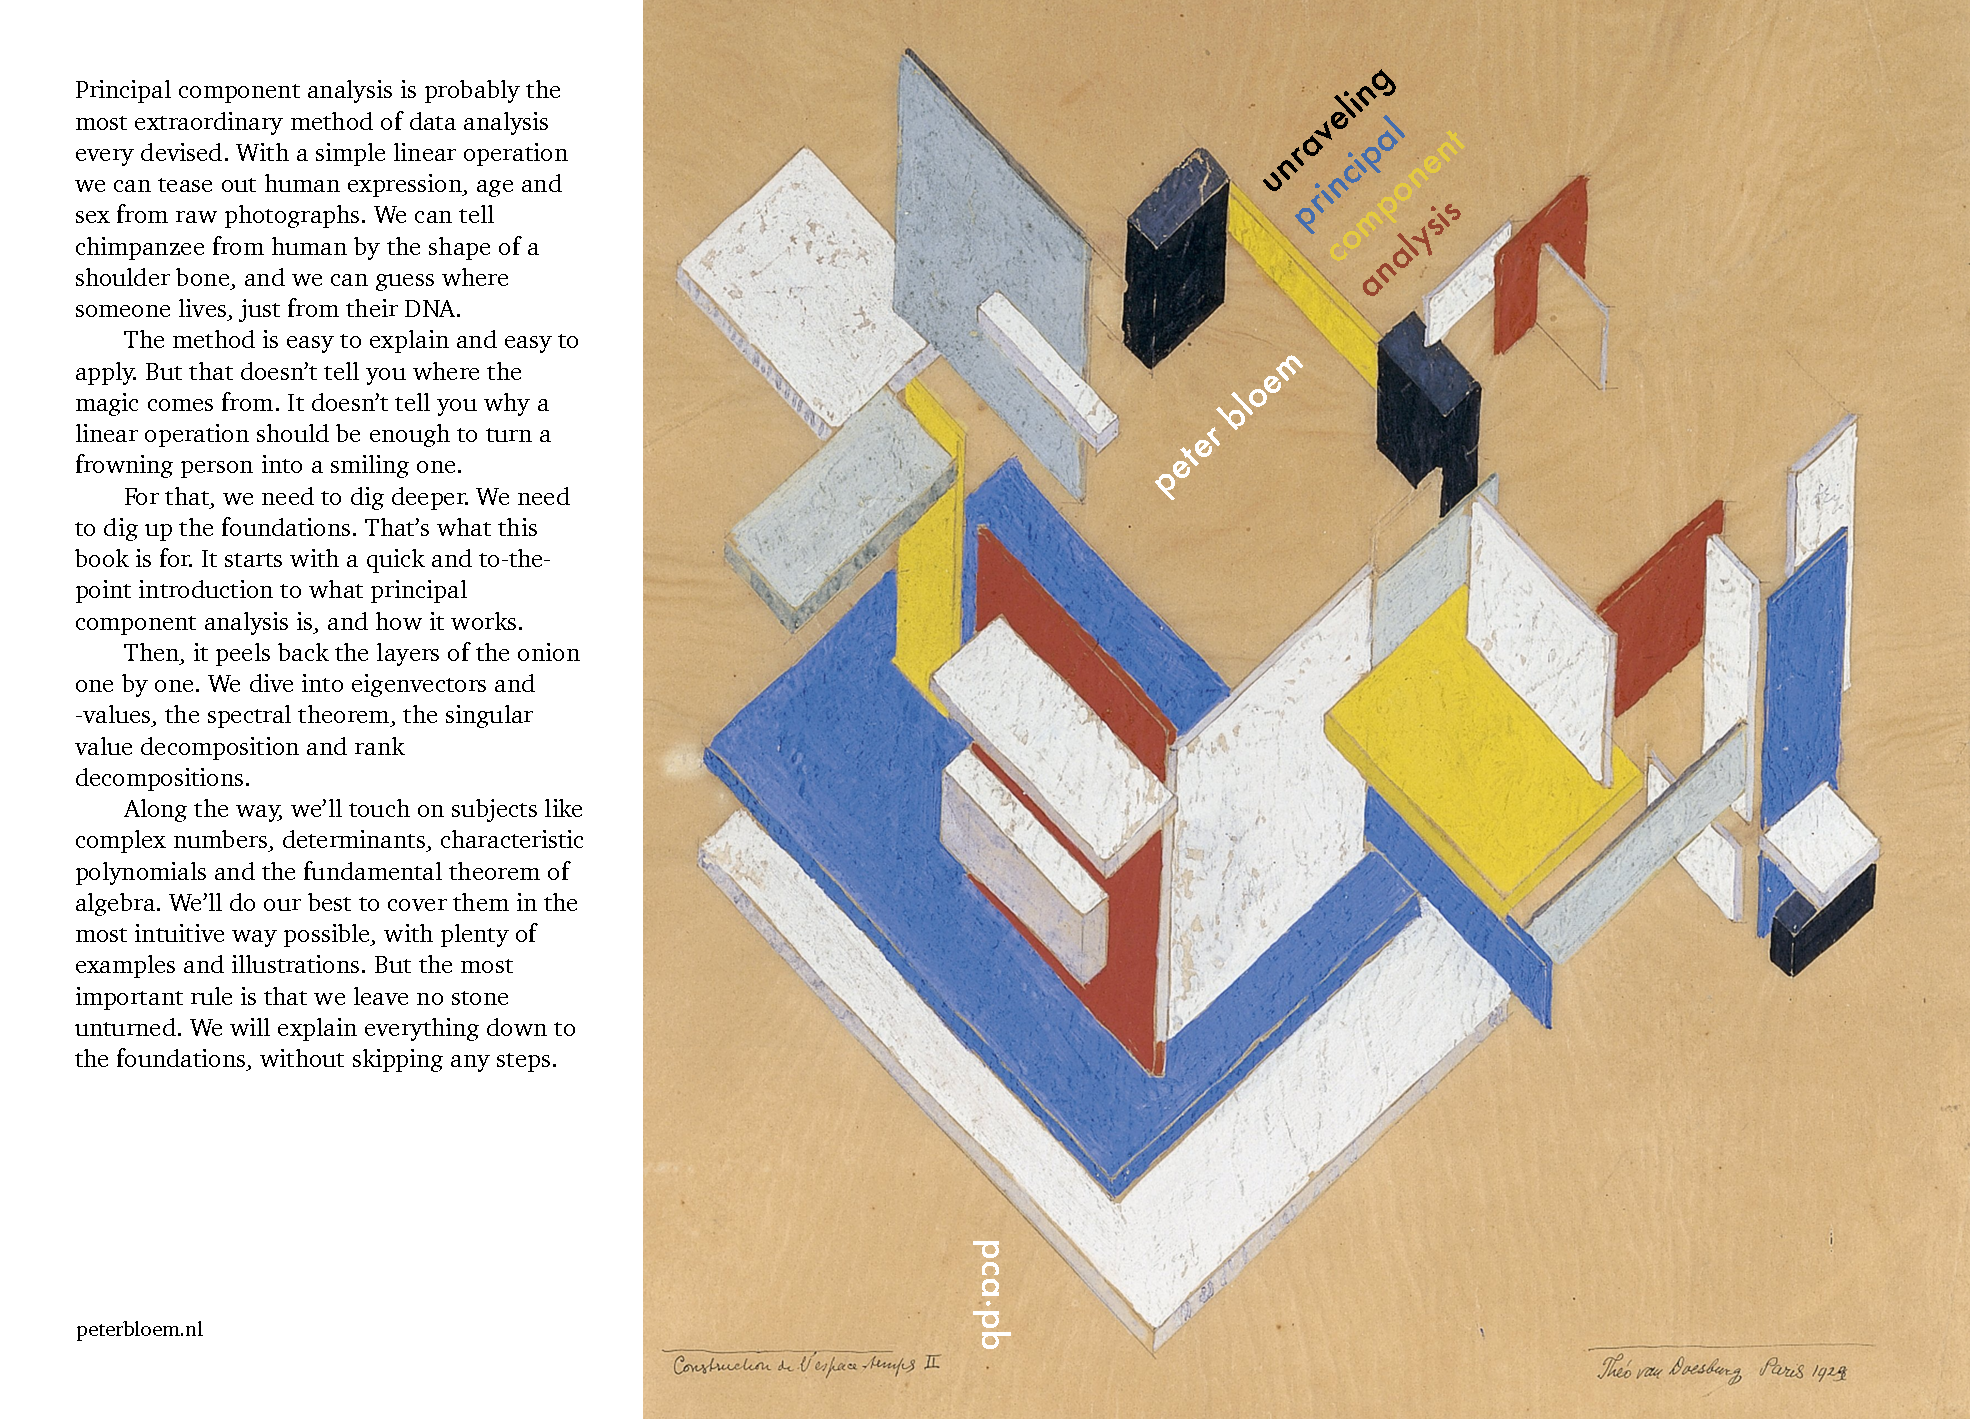
\includepdf[pages=-]{./cover/cover.pdf}
%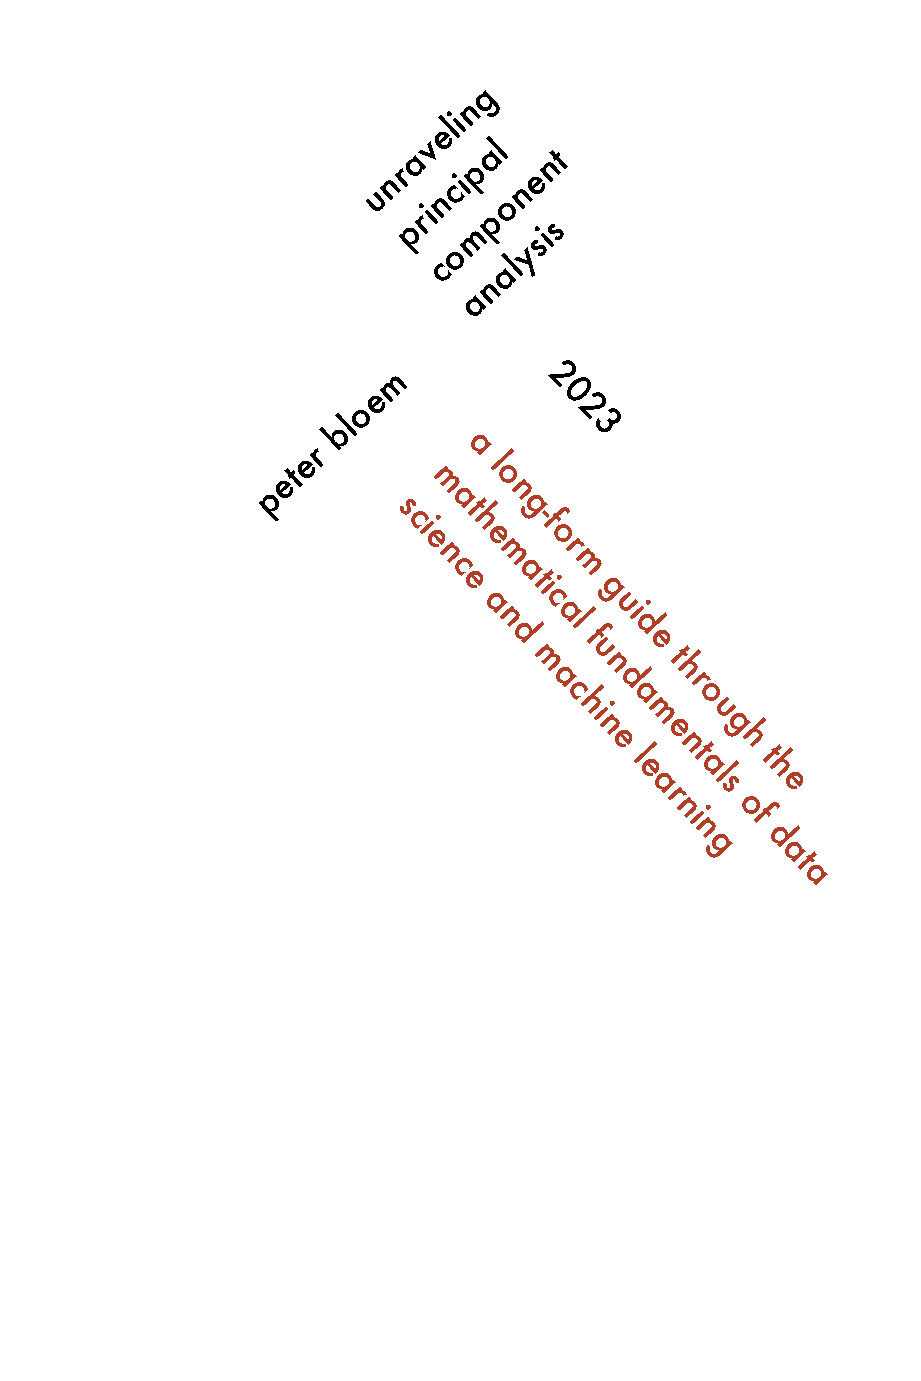
\includepdf[pages=-]{./cover/titlepage.pdf}


\maketitle % Enable for print and replace

\tableofcontents

\cleardoublepage

\chapter*{~}

\vspace{-131pt}

Who is this book for? It wasn't born from a desire to plug a gap in the market, and I didn't have a clear idea of the kind of book I wanted to create when I started. For a long time, it wasn't even meant to be a book. 

It started when I began teaching machine learning in 2018. One of the topics was principal component analysis, and I wanted to do a good job, since it was a topic that had entranced and mystified me in equal measure as a student. I wanted to do it justice.

It turned out that I couldn't do that in the time that was available to prepare a single lecture. On the morning before the lecture, going over my slides I caught several mistakes that I couldn't quite fix, and many questions that I didn't know how to answer.

I brushed it off, survived the lecture despite feeling like an imposter, and resolved to do better next year. The next year, the same thing happened again. Different mistakes, different questions, but the same feeling of cheating myself and the students.

The thing is, as a student, I never delved deeply into the mathematics of anything. I never \emph{really} got to grips with linear algebra and at best, I could only ever claim to have a working grasp of what I needed to apply it in simple settings, and to look up what I didn't know. 

This, I expect, is how it is for many students and researchers alike: we are taught the fundamentals from the ground up, but we only start tuning in when things become concrete. The foundations, we either never learn, or quickly forget.

After three years of this, I decided it was enough, and I began to write a blog post on PCA. This would finally force me to properly come to grips with the subject, however deep the rabbit hole went. Once I was finished, I could use the blog post as part of the teaching material. Proof, if any were need, that I really did know what I was talking about.

The more I wrote, the more questions I generated for myself, and the more the blog post span out of control. I decided to split the thing in two: the first part a simple self-contained story for those, like my students, who just wanted to understand enough of PCA to apply it effectively, and a second part that delved into the fundamentals. 

The pattern continued steadily: to really get down to the foundations, I needed to prove the spectral theorem. This required so many dependencies it became a third blog post, so it didn't clutter up the second. Then, I felt, I needed to end on a clear algorithm for PCA. You can't say you really understand something if you don't know how to implement it. This is always done through the singular value decomposition (SVD), which I then felt I should also understand properly. In the end, the explanation of the SVD and the algorithm to compute it became too big to put into a single blogpost and I split those up too, bringing the tally to five. Five blog posts, with each little too big to function well as a blog post.

In short, I realized I had accidentally written a book. Like I said. I don't really know who it's for. It's about PCA, but it covers much more than that. Almost everything a linear algebra textbook does. But it's not a textbook by any stretch; I certainly wouldn't teach from it, and it kind of assumes you know linear algebra already when you start reading.

It's also not quite popular science. I occasionally go into narrative mode, but really, the aim is to go deep. To dig up the foundations.

 I suppose it's a book for people like me. People who have learned linear algebra and then forgotten it. Who feel a measure of regret that they didn't pay full attention the first time around. If you've ever marveled at the magical results that PCA produces, and you'd like to really understand it, all the way down to the fundament, then this book will provide you with a guide. But perhaps it's best to think of this as a guided tour of the forests of linear algebra. I've been deep into the woods in search of treasure and I've made it back out. Let me show you what I've found.
 
\enlargethispage{2em}
 
\paragraph{Acknowledgements} I am indebted to \href{https://emilevankrieken.com/}{Emile van Krieken} and to Charlie Lu for corrections and suggestions. My thanks go out to Nathan Young for the use of a figure from \citep{young2015fossil} and to John Novembre for useful comments on the interpretation of the genomic PCA analysis in Chapter~\ref{chapter:introduction}.

\paragraph{Licensing} All figures in this book are released under a Creative Commons \href{https://creativecommons.org/licenses/by-sa/2.0/}{CC-BY-SA} license. Source files may be found at \url{https://github.com/pbloem/pca-book}.

%~
%\pagebreak
%~
%\pagebreak

\cleardoublepage

\chapter[A friendly introduction to PCA]{A friendly introduction to principal component analysis}
\label{chapter:introduction}

We will work from the outside in: we will view PCA first as a way of finding a smaller representation of a dataset. This is a typical machine learning problem: find a compressed representation of the data such that the reconstructions are as close to the original as possible. This is a simple view of PCA, an we'll be able to compute it with nothing more than gradient descent with a few extra tricks for satisfying constraints.

Most of the technical stuff only becomes necessary when we want to understand why PCA works so well: this is where the \textbf{spectral theorem} and the \textbf{eigenvalues and -vectors}, come in to the story, they give us a deeper understanding of what we're doing. We'll look at these subjects in Chapter~\ref{chapter:eigenvectors}.

The spectral theorem is the heart of the method, so it pays to discuss it in some detail. We'll state it and explain what it means in Chapter~\ref{chapter:eigenvectors}, and leave the proof to Chapter~\ref{chapter:spectral-theorem}.

%Then, in Chapter~\ref{chapter:svd} we'll look at the the \textbf{singular value decomposition}. This matrix decomposition is not only the most popular method for computing the solutions to PCA, it is also the go-to method for computing many related problems, like least squares fits, and matrix ranks. Finally in Chapter

I'll assume some basic linear algebra knowledge, but  I'll try to explain the preliminaries where possible, even if they are fundamental to linear algebra. There is a small list of identities and properties in the appendix, which you may want to consult to refresh your memory. 

\section{The basics}

Let's begin by setting up some basic notation. We are faced with some high-dimensional dataset of instances (examples of whatever we're studying) described with real-valued features. That is, we have \(\gc{n}\) \emph{instances} \(\mbx_\gc{i}\) and each instance is described by a vector of \(\bc{m}\) real values. We describe the dataset as a whole as an \(\gc{n} \times \bc{m}\) matrix \(\mbX\) that is, we arrange the examples as rows, and the features as columns.

\begin{figure}[H]
	\centerline{
		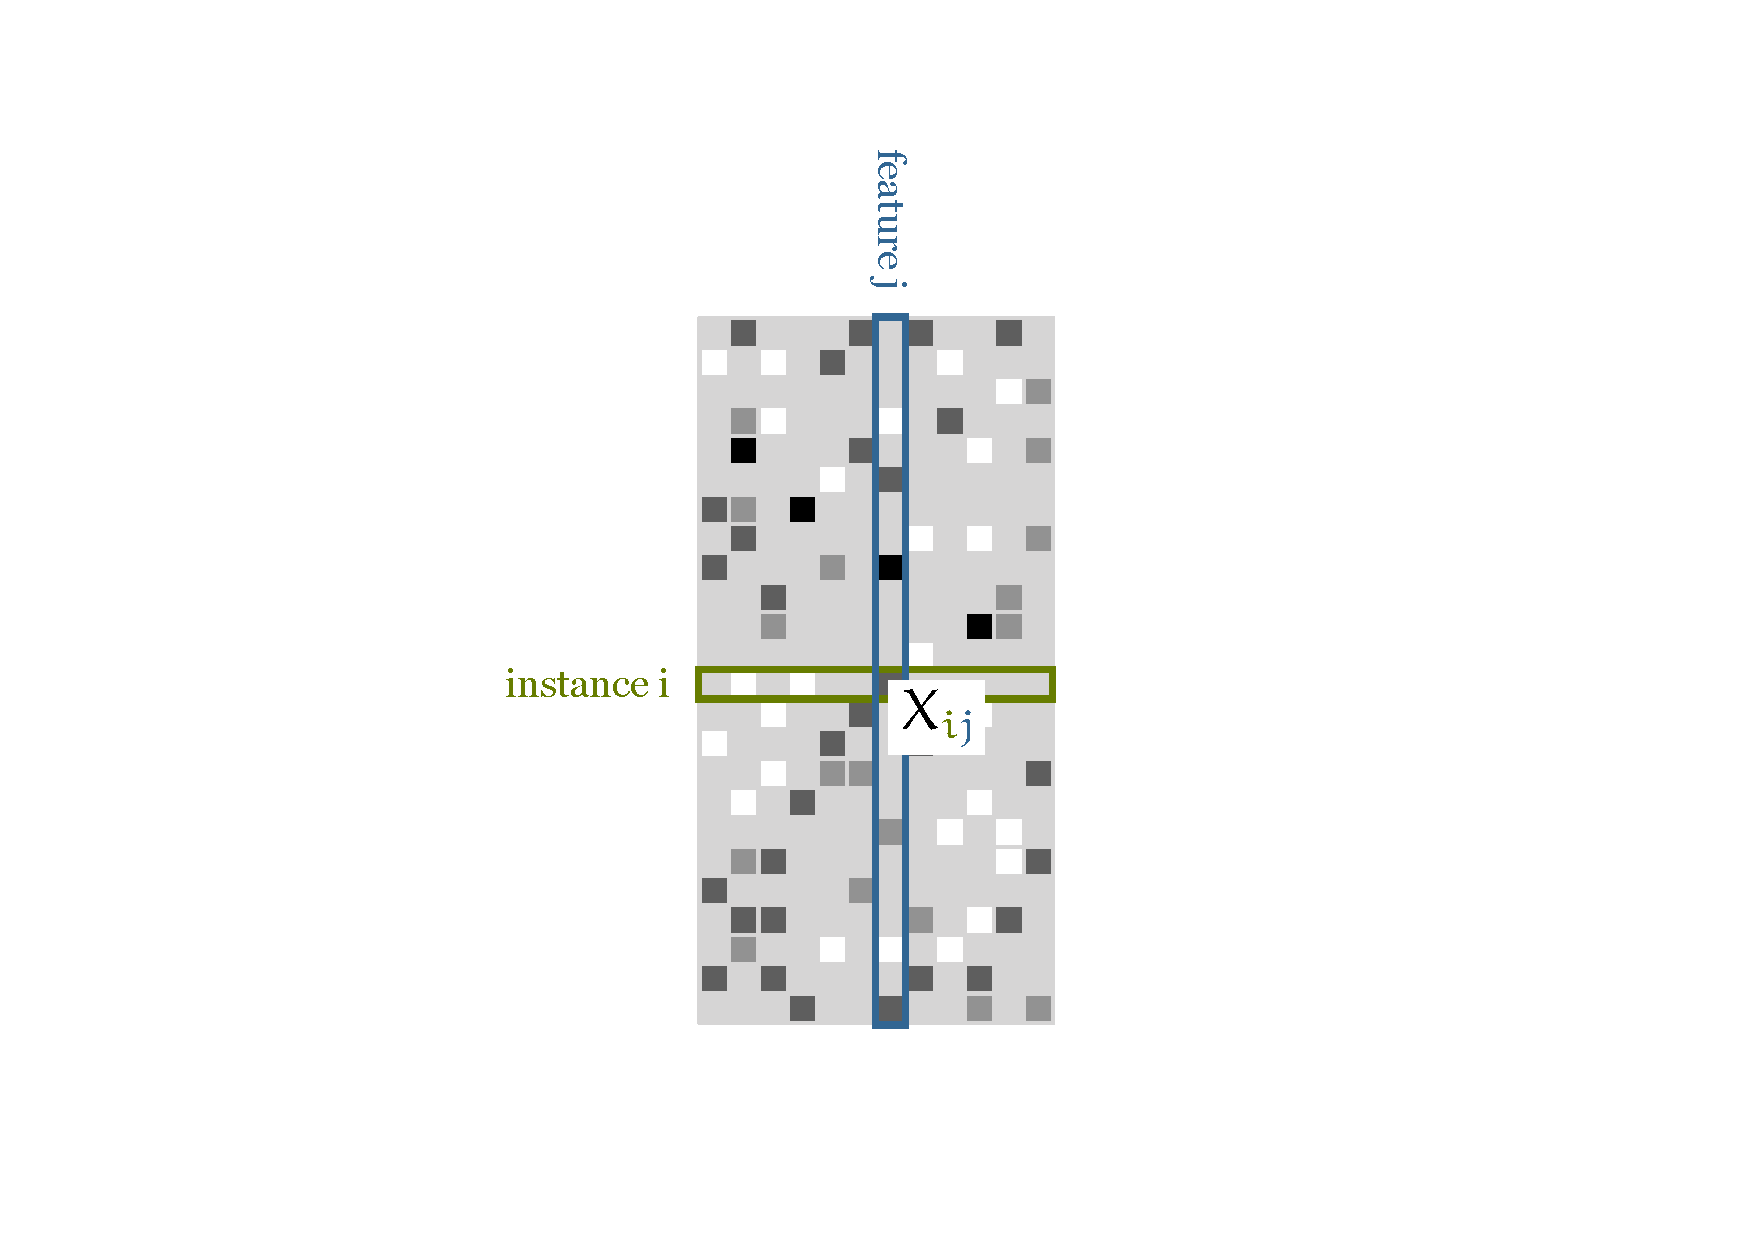
\includegraphics[width=0.6\textwidth]{./images/pca/data-diagram.pdf}
	}
\end{figure}

For a simple example, imagine that we have a dataset of \gc{100 people} with \bc{2 features} measured per person: their monthly salary and their income over the course of a quarter (i.e. three months). The second is just the first times 3, so this data is \emph{redundant}. One value can be computed from the other, so we really only need to store one number per person. Here's what that looks like in a scatterplot.

\begin{figure}[H]
	\centerline{
		\includesvg[width=\textwidth]{./images/pca/income1.svg}
	}
\end{figure}
\vspace{-2em}

\noindent Our intuition that we really only need one number to represent the data is reflected in the fact that \emph{the data form a line}. So long as we know what that line is, we only need to know how far along the line each instance is, so we can store the whole dataset in one number per instance.

\begin{aside}There are also more complex relations between two features that have this property, like a parabola or an exponential curve. In PCA we simplify things by only exploiting linear relations.	
\end{aside}

%
Of course, data in the wild is never this clean. Let's introduce some small variations between the monthly salary and the income after three months. Some people may have changed jobs, some people may get bonuses or vacation allowances, some people may have extra sources of income. Here's a more realistic version of the data.

\vspace{-2em}
\begin{figure}[H]
	\centerline{
		\includesvg[width=\textwidth]{./images/pca/income2.svg}
	}
\end{figure}

\noindent The data is no longer perfectly linear, but it still seems \emph{pretty} linear. If we imagine the same line we had in the last plot, and represent each person as a dot along that line, we lose some information, but we still get a decent \emph{reconstruction} of the data.

If you know how to do linear regression, you can probably work out how to draw such a line through the data, predicting the income from the salary or the other way around (and PCA is very similar to linear regression in many ways). However we'll need something that translates to higher dimensions, where we don't have a single target feature to predict.

\noindent To do so, we'll develop a method purely from these first principles:
\begin{enumerate}
\item We want to represent the data using a small set of numbers per instance.
\item We will limit ourselves to linear transformations of the data to derive this small set.
\item We want to minimize the error in our reconstruction of the data. That is, when we map the data back to the original representation, as best we can, we want it to be as close as possible to the original.
\end{enumerate}

\addvspace{2em}

\section{One-dimensional PCA} % ##
%
We'll develop a one-dimensional version of PCA first. That is, we will represent each instance \(\mbx_\gc{i}\) (row \(\gc{i}\) in our data matrix \(\mbX\)), by a single number \(z_\gc{i}\) as best we can. We will call \(z_\gc{i}\) the \emph{latent representation} of \(\mbx_\gc{i}\).

\begin{aside}The phrase ``latent'' comes from the Latin for \emph{being hidden}. This will make more sense when we see some of the other perspectives on PCA.
\end{aside}

\noindent To start with, we will assume that the data are \textbf{mean-centered}. That is, we have subtracted the mean of the data so that the mean of the new dataset is \(0\) for all features.

\vspace{-1em}
\begin{figure}[H]
	\centerline{
	\includesvg[width=0.9\textwidth]{./images/pca/mean-centered.svg}
	}
\end{figure}
\vspace{-2em}

%<figure class="narrow">
%<img src="/images/pca/mean-centered.svg" />
%</figure>
%
%<aside>
\begin{aside}
For now, think of this as a bit of necessary data pre-processing. We will see where this step comes from in the next chapter.
\end{aside}

Our task is to find a linear transformation from \(\mbx_\gc{i}\) to \(z_\gc{i}\), and another linear transformation back again.
%
A linear transformation from a vector \(\mbx_\gc{i}\) to a single number is just the dot product with a vector of weights. We'll call this vector \(\rc{\mbv}\). A linear transformation from a single number \(z_\gc{i}\) back to a vector is just the multiplication of \(z_\gc{i}\) by another vector of weights. We'll call this vector \(\rc{\mbw}\). This gives us
%
\begin{align*}
z_\gc{i} &= \rc{\mbv}^T \mbx_\gc{i} \\
\mbx'_\gc{i} &= z_\gc{i} \rc{\mbw}
\end{align*}
%
where \(\mbx'_\gc{i}\) is the reconstruction for instance \(\gc{i}\).

Look closely at that second line. It expresses exactly the intuition we stated earlier: we will choose one \rc{line}, represented by the vector \(\rc{\mbw}\), and then we just represent each data point by how far along the line it falls, or in other words, we represent \(\mbx'_\gc{i}\) as a multiple of \(\rc{\mbw}\).

\enlargethispage{3em}

\vspace{-1em}
\begin{figure}[H]
	\centerline{
	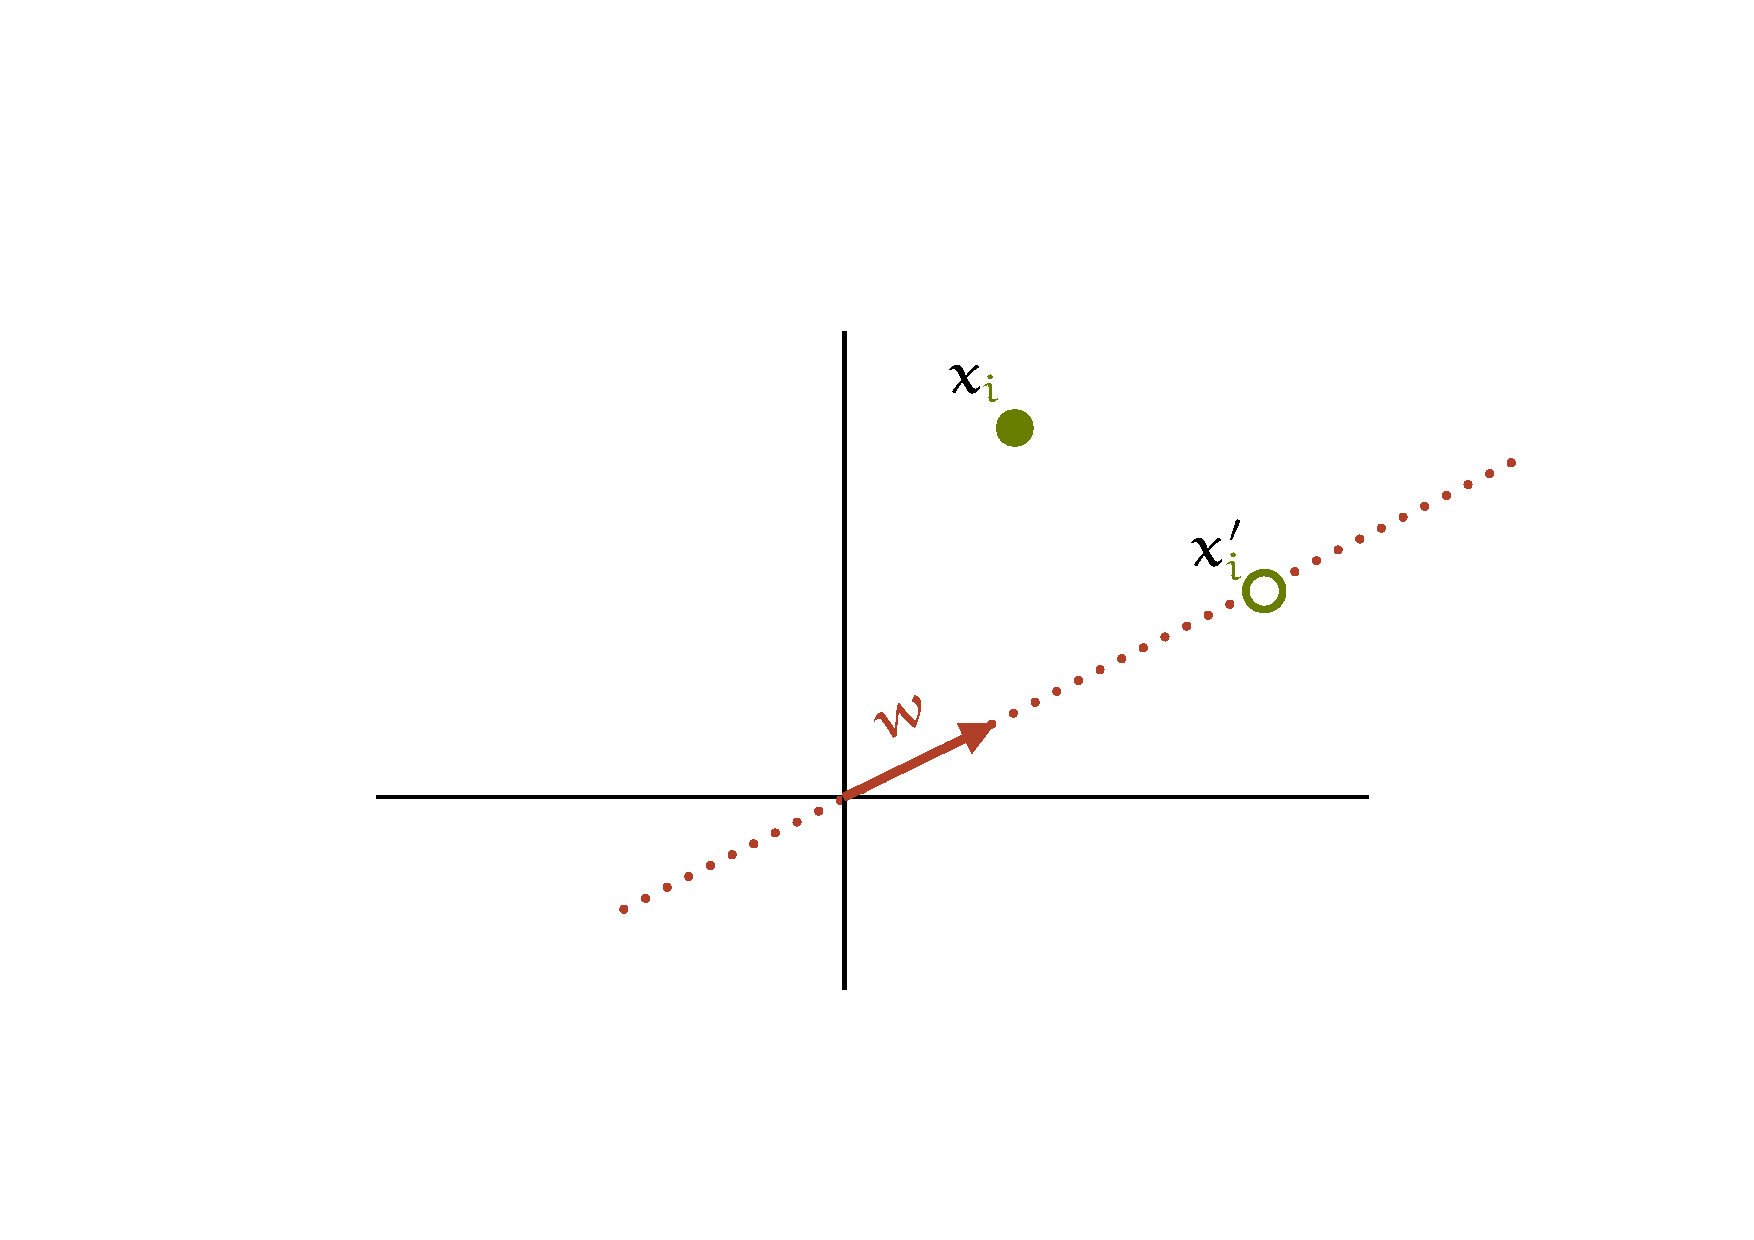
\includegraphics[width=0.8\textwidth]{./images/pca/projection.pdf}
	}
\end{figure}
\vspace{-1em}

%<figure class="narrow">
%<img src="/images/pca/projection.svg" />
%</figure>
%
\noindent All allowed values of \(\mbx'_\gc{i}\) are on the \rc{dotted red line}, which is defined by our choice of \(\rc{\mbw}\). Where each individual ends up is defined by the multiplier \(z_\gc{i}\), wich is determined by the weights \(\rc{\mbv}\). Our objective is to choose \(\rc{\mbv}\) and \(\rc{\mbw}\) so that the reconstruction error, the distance between \(\mbx_\gc{i}\) and \(\mbx'_\gc{i}\) is minimized (over all \(\gc{i}\)).

\vspace{-1em}
\begin{figure}[H]
	\centerline{
		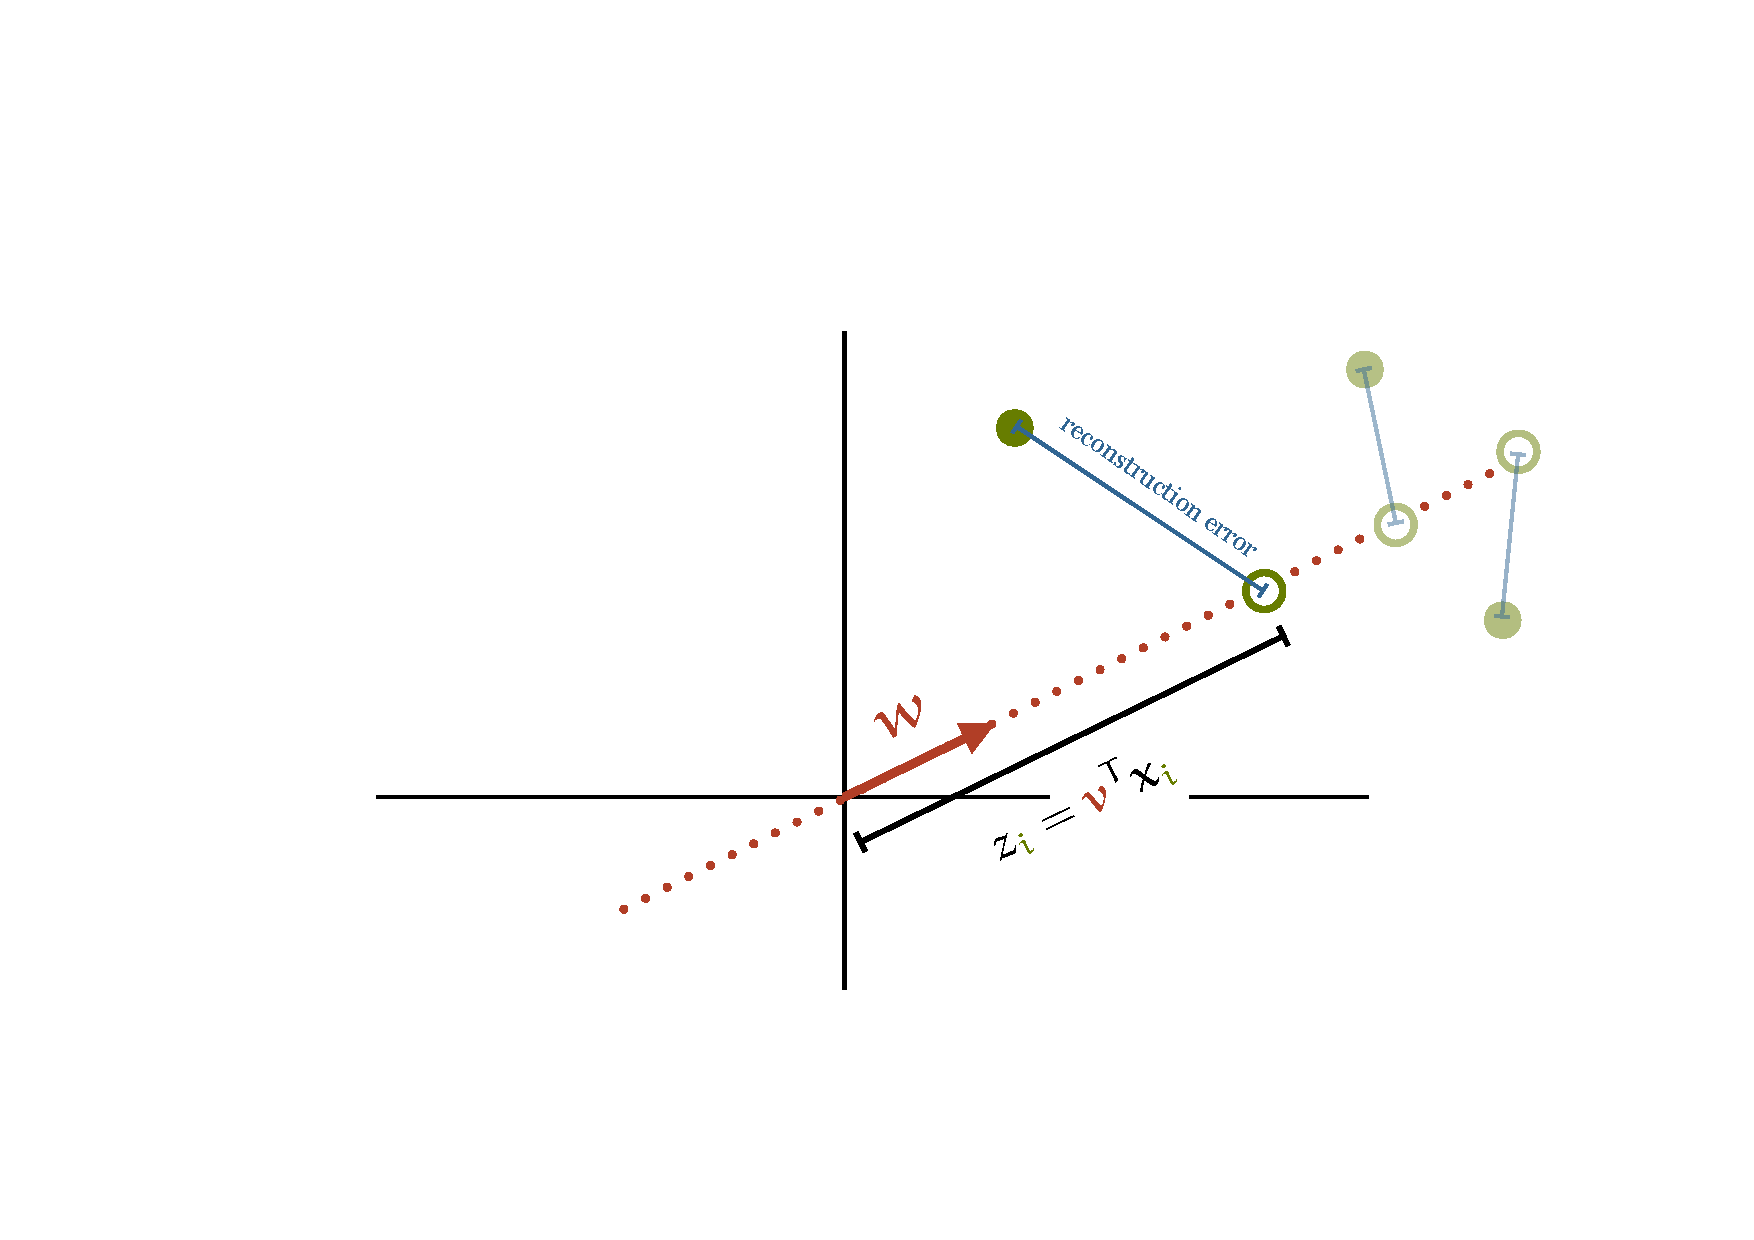
\includegraphics[width=0.8\textwidth]{./images/pca/reconstruction.pdf}
	}
\end{figure}
\vspace{-1em}

%<figure class="narrow">
%<img src="/images/pca/reconstruction.svg" />
%</figure>

\noindent We can simplify this picture in two ways. 

First, note that many different vectors \(\rc{\mbw}\) define the same \rc{dotted line} in the image above. So long as the vector points in the same direction, any length of vector defines the same line, and if we rescale \(z_\gc{i}\) properly, the reconstructed points \(\mbx'_\gc{i}\) will also be the same. To make our solution unique, we will \emph{constrain} \(\rc{\mbw}\) to be a unit vector. That is, a vector with length one: \(\rc{\mbw}^T\rc{\mbw} = 1\).

\begin{aside}
To be more precise, this doesn't leave a unique solution, but two solutions, assuming that a single direction is optimal, since the unit vector can point top right, or bottom left. In other words, if \(\rc{\mbw}\) is a solution, then so is \(-\rc{\mbw}\).
\end{aside}

The second simplification is that we can get rid of the second vector \(\rc{\mbv}\). Imagine that we have  some fixed \(\rc{\mbw}\) (that is, the \rc{dotted line} is fixed). Can we work out which choice of \(\mbx'_\gc{i}\) on the line will minimize the \bc{reconstruction error}? We will go into a bit of detail here, since it helps to set up some intuitions that will be important in the later chapter of this book.

If you remember your linear algebra, you'll know that this happens when the line of the \bc{reconstruction error} is \emph{orthogonal} to the \rc{dotted line}. In more fancy language, the optimal \(\mbx'_\gc{i}\) is the \emph{orthogonal projection} of \(\mbx_\gc{i}\) onto the dotted line. If you look at the image, it's not too difficult to convince yourself that this it true. You can imagine the reconstruction error as a kind of rubber band pulling on \(\mbx'_\gc{i}\), and the point where it's orthogonal is where it comes to rest.

In higher dimensions, however, such physical intuitions will not always save us. Since the relation between orthogonality and least squares is key to understanding PCA, we will take some time to prove this properly.

\begin{theorem}[Best approximation theorem (1D)]
Let \(\rc{\mbw}, \mbx \in \mathbb{R}^n\),  let \(\rc{W}\) be the line of all multiples of \(\rc{\mbw}\), and let \(\rc{\hat \mbw}\) be the orthogonal projection of \(\mbx\) onto \(\rc{W}\). Then, for any other \(\rc{\bar \mbw}\) in \(\rc{W}\), we have 

\[
	\text{dist}(\mbx, \rc{\hat \mbw}) < \text{dist}(\mbx, \rc{\bar \mbw})
\]
where \(\text{dist}(\mba, \mbb)\) denotes the Euclidean distance \(\|\mba - \mbb\|\).
\end{theorem}
\begin{proof}[Adapted from Thm. 9 Ch. 7 in \cite{lay1994linear}] Note that \(\mba - \mbb\) is the vector that points from the tip of \(\mba\) to the bottom of \(\mbb\). We can draw three vectors \(\gc{\bar \mbw - \mbx}\), \(\bc{\hat\mbw -\mbx}\) and \(\rc{\bar \mbw - \hat \mbw}\) as follows:

%\vspace{-1em}

\begin{figure}[H]
	\centerline{
		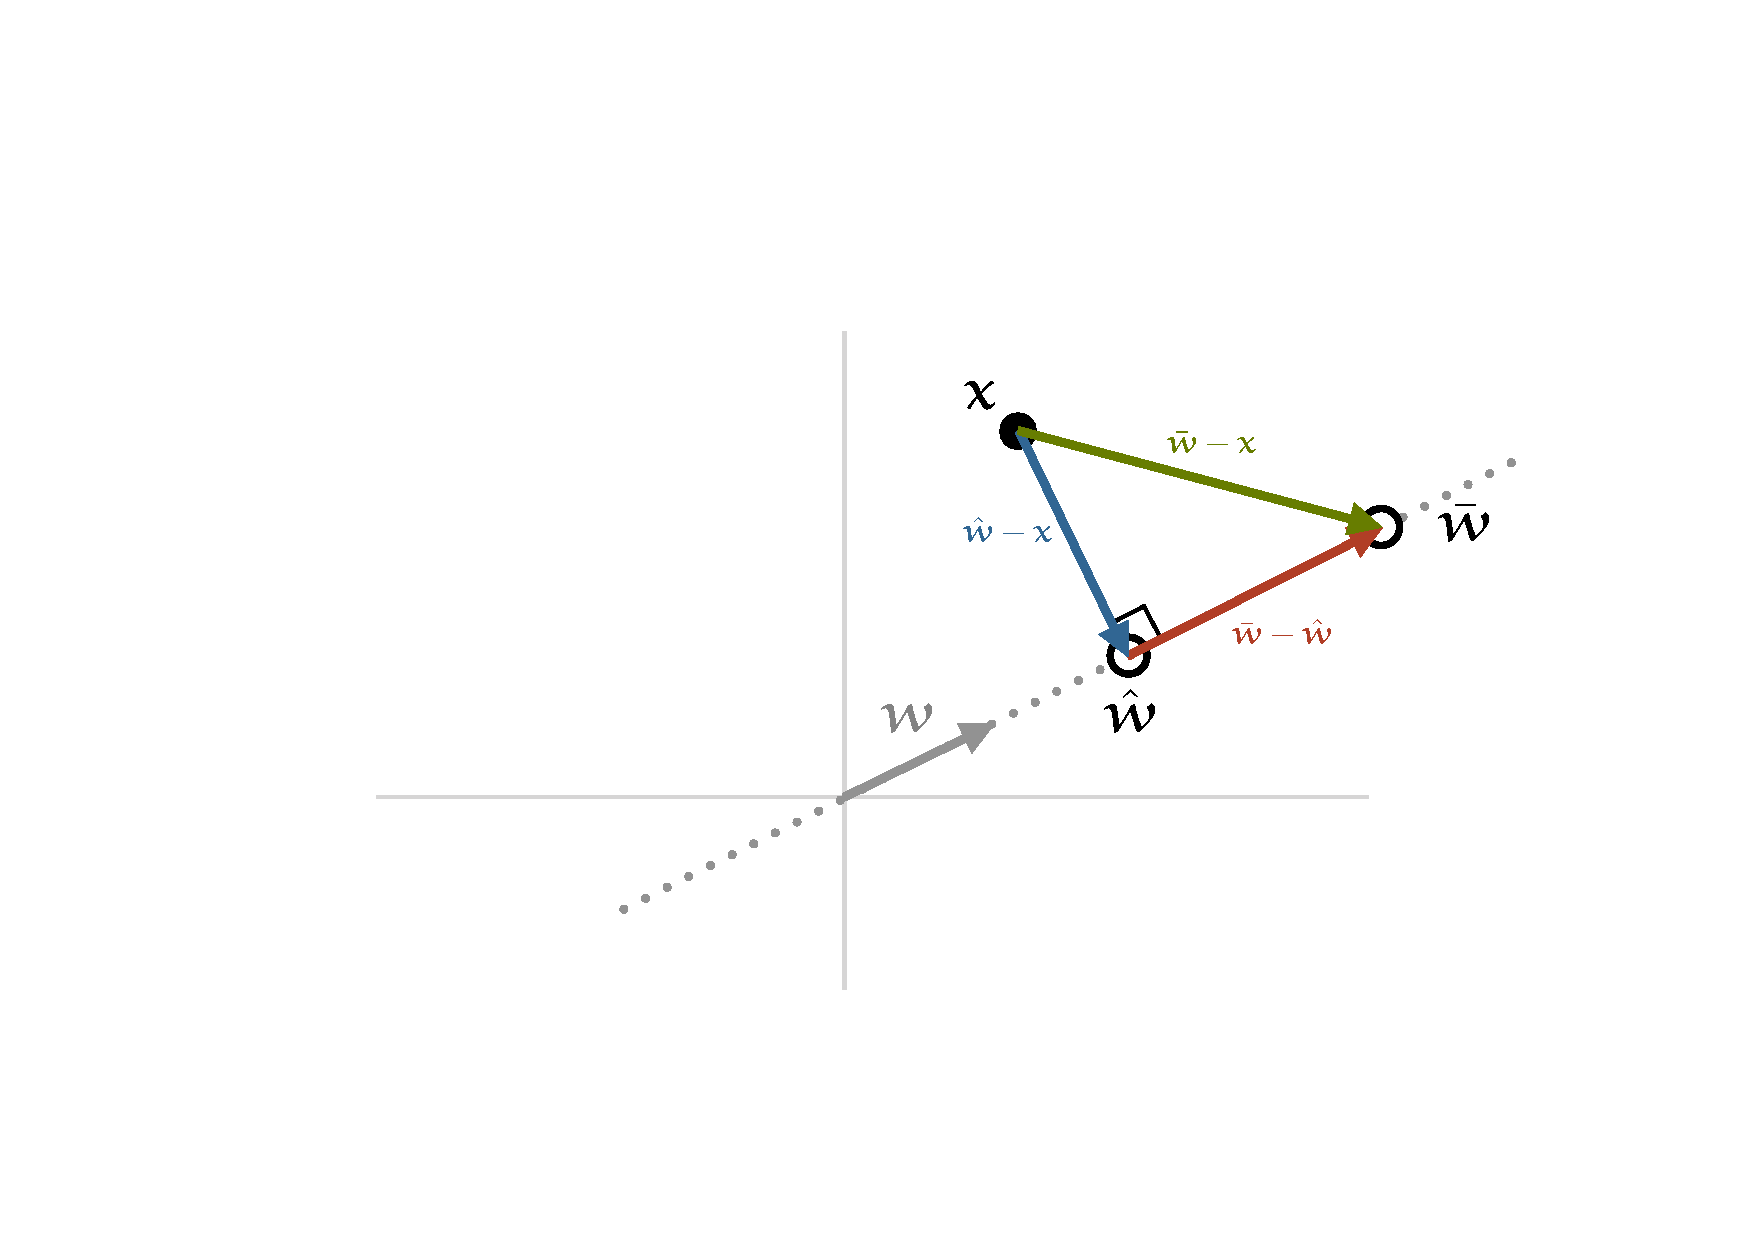
\includegraphics[width=1\textwidth]{./images/pca/pythagoras.pdf}
	}
\end{figure}
%
%\vspace{-1em}

%<figure class="narrow centering">
%<img src="/images/pca/pythagoras.svg" class="three-quarters"/>
%</figure>

By basic vector addition, we know that 

\[
\gc{\bar \mbw - \mbx} = \bc{\hat\mbw -\mbx} + \rc{\bar \mbw - \hat \mbw} \text{,}
\]

\textbf{so the three vectors form a triangle} (when we arrange them as shown in the picture).

We also know, by construction, that \(\bc{\hat\mbw -\mbx}\) is orthogonal to \(\rc{\bar \mbw - \hat \mbw}\), so \textbf{the triangle is right-angled}.

Since we have a right angled triangle, the Pythagorean theorem tells us that the lengths of the sides of the triangles are related by

\[
\gc{\text{dist}(\mbx, \bar \mbw)}^2 = \bc{\text{dist}(\hat \mbw, \mbx)}^2+ \rc{\text{dist}(\bar \mbw, \hat \mbw)}^2 \p
\]

Since \(\rc{\text{dist}(\bar \mbw, \hat \mbw)} > 0\) (because \(\bar \mbw\) and \(\hat \mbw\) are not the same point), we know that \(\gc{\text{dist}(\mbx, \bar \mbw)}\) must be strictly larger than \(\bc{\text{dist}(\hat \mbw, \mbx)}\). \hfill\qedsymbol
\end{proof}


\begin{aside}This result generalizes easily to any linear subspace \(\rc{W}\) spanned by a given set of vectors. We will show a more general proof in Chapter~\ref{chapter:svd}. This principle, the orthogonal projection as the best approximation is at the heart of a lot of optimization problems.
\end{aside}

So, the best reconstruction \(\mbx'_\gc{i}\) of the point \(\mbx_\gc{i}\) on the line defined by \(z \cdot \rc{\mbw}\) (however we choose \(\rc{\mbw}\)) is the orthogonal projection of \(\mbx_\gc{i}\) onto \(\rc{\mbw}\). So how do we compute an orthogonal projection? Let's look at what we have:

\vspace{-1em}
\begin{figure}[H]
	\centering
	\includesvg[width=1\textwidth]{./images/pca/projection2.svg}
\end{figure}
\vspace{-1em}

%<figure class="narrow centering">
%<img src="/images/pca/projection2.svg" class="three-quarters"/>
%</figure>

\noindent We've projected \(\mbx_\gc{i}\) down onto \(\rc{\mbw}\) and we've given the vector from the projection to the original the name \(\bc{\mbr}\). By vector addition we know that \(z\rc{\mbw} + \bc{\mbr} = \mbx_\gc{i}\), so \(\bc{\mbr} = \mbx_\gc{i} - z\rc{\mbw}\).


\pagebreak

\noindent Two vectors are orthogonal if their dot product is zero, so we're looking for a \(z\) such that \(z\rc{\mbw}^T\bc{\mbr} = 0\), or equivalently, \(\rc{\mbw}^T\bc{\mbr} = 0\). We rewrite

\[
0 = \rc{\mbw}^T\bc{\mbr} = \rc{\mbw}^T\left(\mbx_\gc{i} - z\rc{\mbw}\right) = \rc{\mbw}^T\mbx_\gc{i} - z\rc{\mbw}^T\rc{\mbw} \p
\]

This gives us \(z = \rc{\mbw}^T\mbx_\gc{i} / \rc{\mbw}^T\rc{\mbw}\). And, since we'd already defined \(\rc{\mbw}\) to be a unit vector (so \(\rc{\mbw}^T\rc{\mbw} = 1\)), we get \(z = \rc{\mbw}^T\mbx_\gc{i}\).

Let's retrace our steps. We had two weight vectors: \(\rc{\mbv}\) to encode \(\mbx_\gc{i}\) into the single number \(z_\gc{i}\), and \(\rc{\mbw}\) to decode \(\mbx_\gc{i}\) as \(z_\gc{i}\rc{\mbw}\). We've now seen that for any given \(\rc{\mbw}\), the best choice of \(z_\gc{i}\) is \(\rc{\mbw}^T\mbx_\gc{i}\). In other words, \textbf{we can set \(\rc{\mbv}\) equal to \(\rc{\mbw}\) and use it to encode and to decode}.

\begin{aside}
Note that an important requirement for this result (and its generalizations coming up) is  that \(\rc{\mbw}\) is a unit vector.
\end{aside}

So, after all that, we can finally state precisely what we're looking for. Given \(\rc{\mbw}\) our reconstruction is \(\mbx'_\gc{i} = z_\gc{i} \cdot \rc{\mbw} = \oc{\mbw^T\mbx_i \cdot \mbw}\). This means we can state our goal as the following constrained optimization problem:

\begin{align*}
&\argmin{\rc{\mbw}} \sum_\gc{i} \| \oc{\mbw^T\mbx_i \cdot \mbw}  - \mbx_\gc{i} \| \\
&\;\;\;\;\text{such that } \rc{\mbw}^T\rc{\mbw} = 1 \p
\end{align*}

How do we solve this? This is a simple problem and there are fast ways to solve it exactly. But we've done a lot of math already, and it's time to show you some results, so we'll just solve this by gradient descent for now. Basic gradient descent doesn't include constraints, but in simple cases like these, we  can use \emph{projected} gradient descent: after each gradient update, we project the parameters back to the subset of parameter space that satisfies the constraint (in this case simply by dividing \(\rc{\mbw}\) by its length).

\begin{aside}If you don't know \href{https://mlvu.github.io/lecture02/}{how gradient descent works}, you can just imagine a procedure that starts with a random choice for \(\rc{\mbw}\) and takes small steps in the direction that the function above decreases the most.
\end{aside}

We start by initializing \(\rc{\mbw}\) to some arbitrary direction. Here's what the projections of the income data onto that \(\rc{\mbw}\) look like.

%\vspace{-1em}
\begin{figure}[H]
	\centerline{
	\includesvg[width=0.899\textwidth]{./images/pca/random-w.svg}
	}
\end{figure}
%\vspace{-1em}

%<figure class="narrow">
%<img src="/images/pca/random-w.svg" />
%</figure>

The (squared) sum of the lengths of the \bc{blue lines} is what we want to minimize. Clearly, there are better options than this choice of \(\rc{\mbw}\). After a few iterations of gradient descent, this is what we end up with.

%\vspace{-1em}
\begin{figure}[H]
	\centerline{
	\includesvg[width=0.899\textwidth]{./images/pca/sol-w.svg}
	}
\end{figure}
%\vspace{-1em}

You can think of the blue lines of the reconstruction error as pulling on the line of \(\rc{\mbw}\) and of \(\rc{\mbw}\) as pivoting on the origin.
\pagebreak 

\noindent For any dataset (of however many dimensions), there is a unique, optimal line \(\rc{\mbw}\). It's called the \textbf{first principal component}.

\begin{aside}
If you've read other descriptions of PCA, you may be wondering at this point why I'm not talking about maximizing the variance. This is an alternative way to define PCA. We'll discuss it in the next chapter.
\end{aside}

What can we say about the meaning of the elements of \(\rc{\mbw}\)? Remember that it does two things: it encodes from \(\mbx\) to \(z\) and it decodes from \(z\) to \(\mbx'\). The encoding is a dot product: a weighted sum over the elements of \(\mbx\).

In the first example of the income data, before we added the noise, the second feature was always exactly three times the first feature. In that case, we could just remember the first feature, and forget the second. That would be equivalent to encoding with the vector \(\rc{(1, 0)}\). The compressed representation \(z\) would be equivalent to the first feature and we could decode with \(z \times\rc{(1, 3)}\). Or, we could encode with \(\rc{(0, 1)}\) and decode with \(\rc{(\tfrac{1}{3}, 1)}\).

Why are the encoding and decoding vectors different in these cases? Because when we proved that they were the same, we assumed that they were unit vectors. Our encoding vector is a unit vector, but the corresponding decoding vector isn't. PCA provides solution for which the encoder and the decoder are the same. It takes a mixture of both features, in different proportions (in our case \(1/\sqrt{10}\) and \(3/\sqrt{10}\)) . There are a a lot of perspectives on exactly what this mixture means. We'll illustrate the first by looking at a higher dimensional dataset.

We'll use a dataset of grayscale images of faces produced by AT\&T Laboratories Cambridge called the \emph{Olivetti dataset}.\footnotemark 

\footnotetext{\url{https://scikit-learn.org/stable/datasets/real_world.html\#the-olivetti-faces-dataset}}

\begin{figure}[t]
	\centerline{
	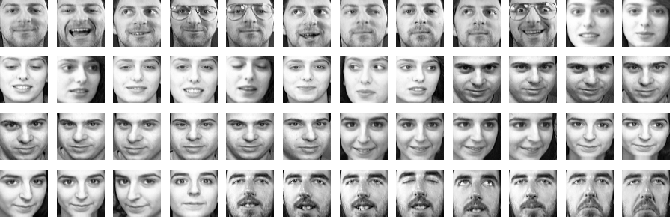
\includegraphics[width=1.2\textwidth]{./images/pca/faces.png}}
	\caption*{A small sample of images from the Olivetti data.}
\end{figure}
%\vspace{-1em}

%<figure class="narrow">
%<img src="/images/pca/faces.png" />
%</figure>

We will describe each pixel as a feature with a value between 0 (black) and 1 (white). The images are \(64 \times 64\) pixels, so each image can be described as a single vector of \bc{\(4096\) real values}.

\begin{aside}Note that by flattening the images into vectors we are entirely ignoring the grid structure of the features: we are not telling our algorithm whether two pixels are right next to each other, or at opposite ends of the image.
\end{aside}

The Olivetti data contains \gc{400 images}, so we end up with a data matrix \(\mbX\) of 
\(\gc{400} \times \bc{4096}\). 

\begin{figure}[H]
	\centering
	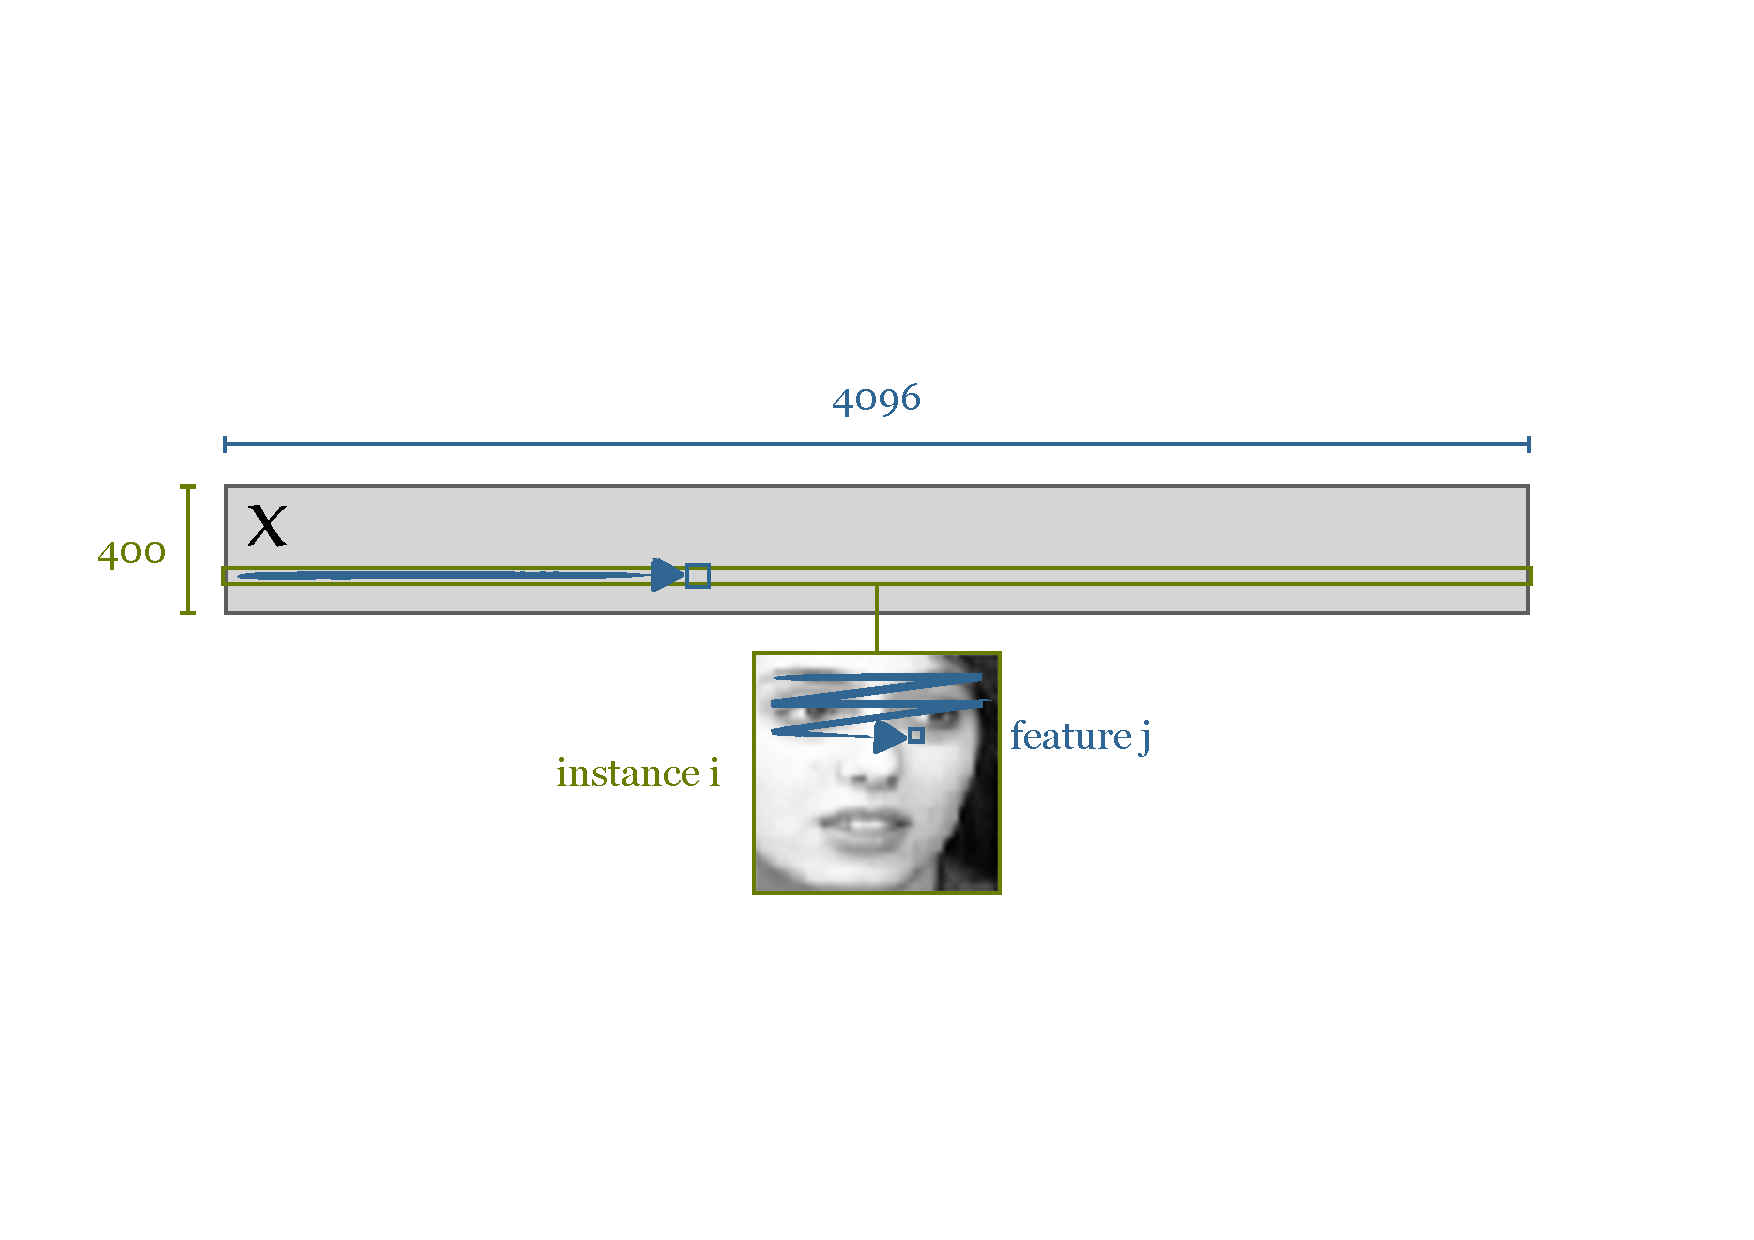
\includegraphics[width=1\textwidth]{./images/pca/images-diagram.pdf}
\end{figure}

%<figure class="narrow">
%<img src="/images/pca/images-diagram.svg" />
%</figure>

This is a data scientist's worst nightmare: data with many more features than instances. With so many features, the space of possible instances is vast, and we only have a tiny number to learn from. Our saving grace is that, like the income/salary example, the features in this dataset are highly \emph{dependent}: knowing the value of one pixel allows us to say a lot about the value of other pixels. 

For instance, pixels that are close together more often than not have similar values. The images are often roughly symmetric. All faces will have mostly uniform patches of skin in roughly the same place, and so on. 

In short, while our dataset is expressed in \bc{4096} dimensions, we can probably express the same information in many fewer numbers, especially if we are willing to trade off a little accuracy for better compression.

The procedure we will use to find the first principal component for this data is exactly the same as before---search for a unit vector that minimizes the reconstruction loss---except now the instances have \bc{4096} features, so \(\rc{\mbw}\) has \bc{4096} dimensions. First, let's look at the reconstructions.

\begin{figure}[H]
	\centerline{
	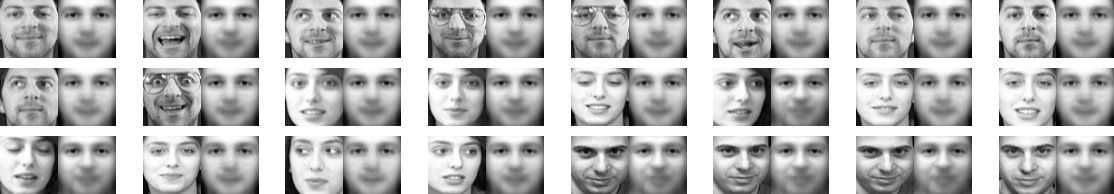
\includegraphics[width=1.4\textwidth]{./images/pca/face-reconstructions.png}
	}
	\caption*{Reconstruction from a single principal component. Originals on the left, reconstructions on the right.}
\end{figure}

%<figure class="wide-margin">
%<img src="/images/pca/face-reconstructions.png"/>
%</figure>

These are not very impressive yet, but to be fair, we've compressed each image into a single number, we shouldn't be surprised that there isn't much left after we reconstruct it. But that doesn't mean that 1D PCA doesn't offer us anything useful. 

What we can do is look at the first principal component in data space: \(\rc{\mbw}\) is a vector with one element per pixel, so we can re-arrange it into an image and see what each element in the vector tells us about the original pixels of the data. We'll color the positive elements of \(\rc{\mbw}\) red and the negative values blue.

\enlargethispage{4em}

It looks like this:

\begin{figure}[H]
	\centering
	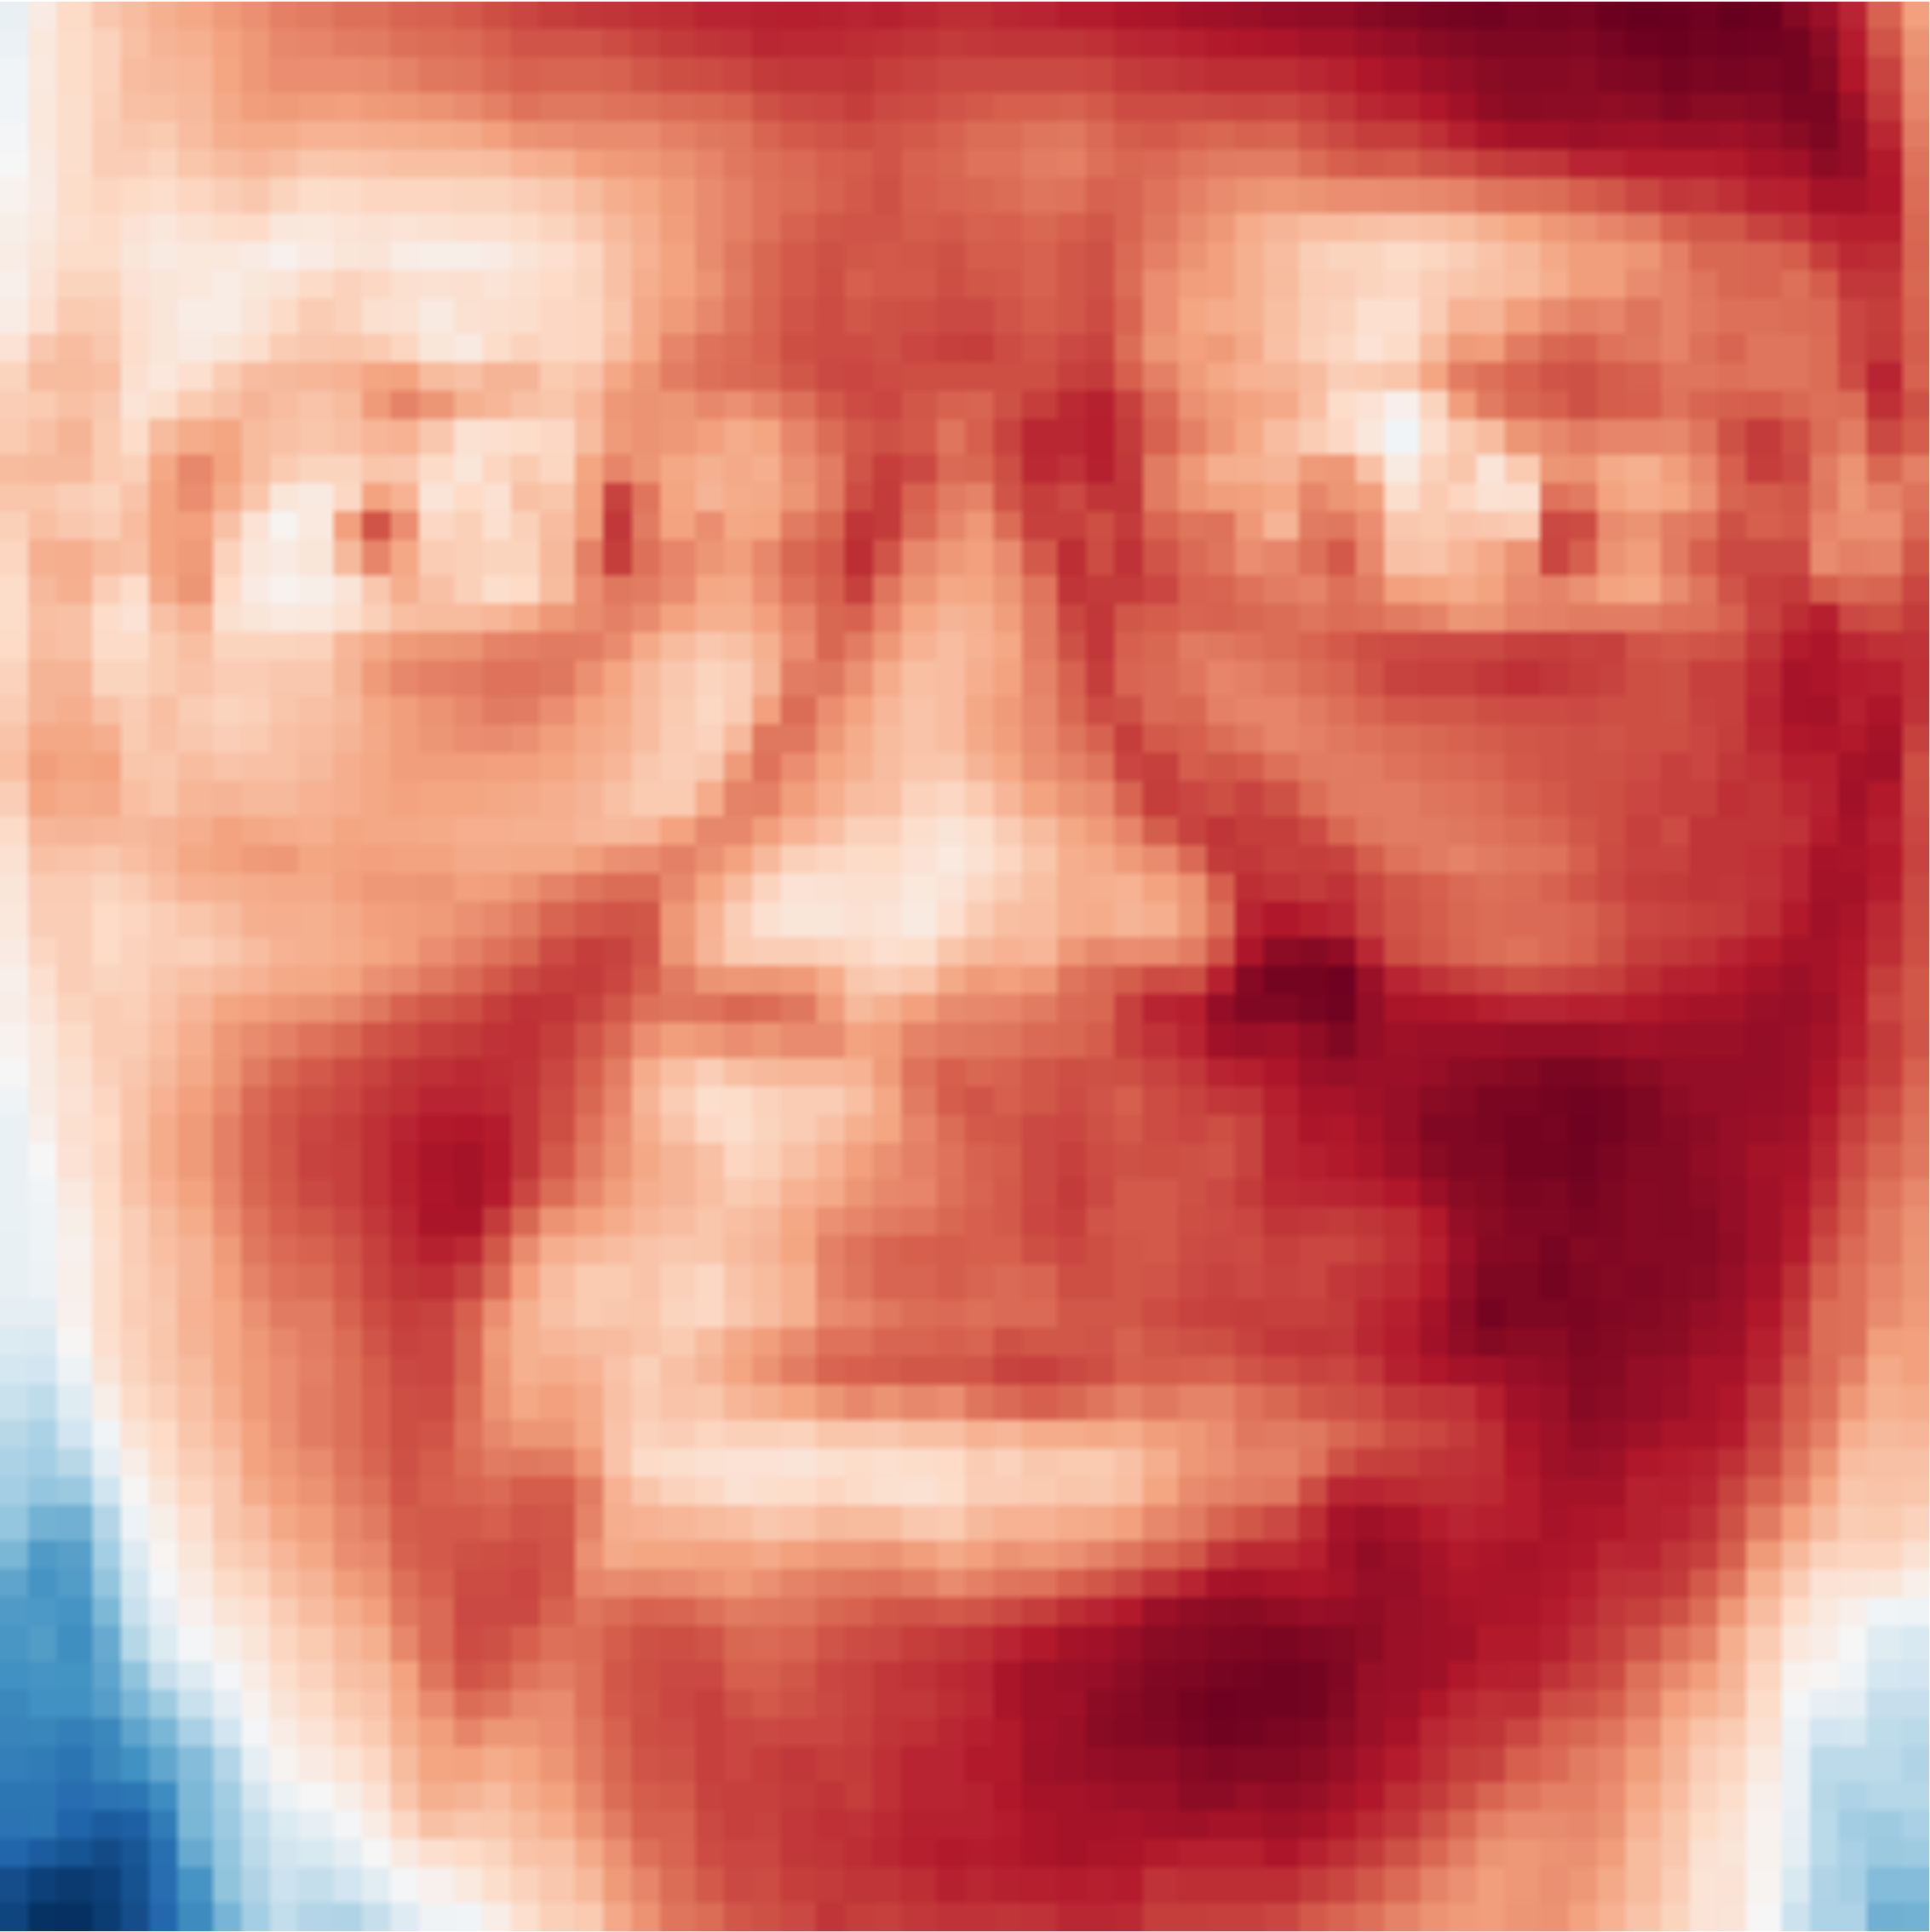
\includegraphics[width=0.4\textwidth]{./images/pca/firstpc.png}
\end{figure}

\noindent If we think of this as the \emph{encoding} vector, we can see a heatmap of which parts of the image the encoding looks at: the darker the red, the more the value of that pixel is added to \(z\). The darker the blue, the more it is subtracted. 

If we think of this as the \emph{decoding} vector, we can see that the larger \(z\) is, the more of the red areas gets added to the decoded image, but the more of the blue areas get \emph{subtracted}. That is, two red pixels are positively correlated, and a red and a blue pixel are negatively correlated. A bright red pixel and a light red pixel have the same relation as our monthly salary and quarterly income: one is (approximately) a multiple of the other.

%\begin{aside}
%If you rerun the code yourself, you may get the same images with blues and reds reversed. Remember that there are two solutions, one the negative of the other.
%\end{aside}

Another interpretation of the principal component is that it places the images in the dataset on a single line, which mean it orders the images along a single direction.

To see if there's any interpretable meaning to this ordering, we can try moving along the line and decoding the points we find. We can start at the origin (the vector \(\mathbold 0\)). If we decode that, we get the mean of our dataset (the so called mean face). By adding or subtracting a little bit of the principal component, we can see what happens to the face.

\begin{figure}[H]
	\centerline{
	\includesvg[width=1.2\textwidth]{./images/pca/int-mean-face.svg}
	}
\end{figure}

%<figure class="wide-margin">
%<img src="/images/pca/int-mean-face.svg"/>
%</figure>

A few things are happening at once: the skin is becoming less clear, the lines in the face become more pronounced, the glasses become more pronounced and the mouth curves upward. Most of this is consistent with moving from a young subject to an old one. 

We can test this on the faces in our dataset as well; our principal component is a direction in the data space, so we can start with an image from our data, and take small steps in the direction of the principal component, or in the opposite direction.

\begin{aside}%
You can think of this as manipulating the single-number latent representation \(z\) by adding some small amount \(\epsilon\). If we decode such a point, we get \((z+\epsilon)\rc{\mbw} = z\rc{\mbw} + \epsilon\rc{\mbw} = \mbx' + \epsilon\rc{\mbw}\). We then just replace the reconstruction \(\mbx'\) by the actual point \(\mbx\). Note that we depend on the linearity of our transformation: for nonlinear variants of PCA, this trick won't work anymore.
\end{aside}

Here's what we get.

\begin{figure}[H]
	\centerline{
	\includesvg[width=1.2\textwidth]{./images/pca/int-data-faces.svg}
	}
\end{figure}

%<figure class="wide-margin">
%<img src="/images/pca/int-data-faces.svg"/>
%</figure>

Note the manipulation of the mouth, in particular in face 41. As the corners of the mouth go up, the bottom lip goes from curving outward, with a shadow under the lip to curving inwards, folding under the teeth, with the shadow turning into a highlight.

\noindent Here we see the real power of PCA. While the reconstructions may not yet be much to write home about, the principal component itself allows us, using nothing but a linear transformation consisting of a single vector, to perform realistic manipulation of facial data, based on a dataset of just 400 examples.

\section{n-Dimensional PCA}

Enough playing around in a one-dimensional latent space. What if we want to improve our latent representations by giving them a little more capacity? How do we do that in a way that gives us better reconstructions, but keeps the meaningful directions in the latent space? 

Let's start by updating our notation. \(\mbx_\gc{i}\) is still the same vector, row \(\gc{i}\) in our data matrix \(\mbX\), containing \(\bc{m}\) elements, as many as we have features. \(\mbz_\gc{i}\) is now also a vector (note the boldface). \(\mbz_\gc{i}\) has \(\rc{k}\) elements, where \(\rc{k}\) is the number of latent features, a parameter we set. In the example above, \(\rc{k}=1\). We'll drop the \(\gc{i}\) subscript to clarify the notation.

\noindent Let's say we set \(\rc{k}=2\). If we stick to the rules we've followed so far---linear transformations by unit vectors---we end up with the following task: find two unit vectors \(\rc{\mbw}_\rc{1}\) and \(\rc{\mbw}_\rc{2}\) and define \(\mbz = (z_\rc{1}, z_\rc{2})\) by \(z_\rc{1} = \mbx ^T\rc{\mbw}_\rc{1}\) and \(z_\rc{2} = \mbx^T \rc{\mbw}_\rc{2}\). Each latent vector gives us a reconstruction of \(\mbx\). We sum these together to get our complete reconstruction.

We can combine the two vectors \(\rc{\mbw_1}\) and \(\rc{\mbw_2}\) in a single matrix \(\rc{\mbW}\) (as its columns) and write

\begin{align*}
\mbz &= \rc{\mbW}^T\mbx \\
\mbx' &= \rc{\mbW}\mbz
\end{align*}

Or, in diagram form:

\vspace{-1.5em}
\begin{figure}[H]
	\centering
	\includesvg[width=0.4\textwidth]{./images/pca/multiplication-nd.svg}
\end{figure}
\vspace{-1.5em}

%<figure class="narrow centering">
%<img src="/images/pca/multiplication-nd.svg" class="half"/>
%</figure>

\noindent This would already work fine as a dimensionality reduction method. You can think of this as an autoencoder, if you're familiar with those. However, we can add one more rule to improve our reduced representation. \textbf{We will require that \(\rc{\mbw_2}\) is orthogonal to \(\rc{\mbw_1}\).}

\begin{aside}%
This decision is important, and has many useful consequences. We'll save those for later. For now, we'll just take it at face value.
\end{aside}

In general, each component \(\rc{\mbw}_r\) we add should be orthogonal to all components before it: for \(\rc{k} = 3\) we add another unit vector \(\rc{\mbw_3}\), which should be orthogonal to both \(\rc{\mbw_1}\) and \(\rc{\mbw_3}\).

We can summarize these constraints neatly in one matrix equation: the matrix \(\rc{\mbW}\), whose columns are our \(\rc{\mbw}\) vectors, should satisfy:

\[
\rc{\mbW}^T\rc{\mbW} = \mbI
\]
%
where \(\mbI\) is the \(\rc{k} \times \rc{k}\) identity matrix. This equation combines both of our constraints: unit vectors, and mutually orthogonal vectors. On the diagonal of \(\rc{\mbW}^T\rc{\mbW}\), we get the dot product of every column of \(\rc{\mbW}\) with itself (which should be \(1\) so that it is a unit vector) and off the diagonal we get the dot product of every column of \(\rc{\mbW}\) with every other column (which should be \(0\), so that they are orthogonal).

How do we find our \(\rc{\mbW}\)? The objective function remains the same: the sum of squared distances between the instances \(\mbx\) and their reconstructions \(\mbx'\). To satisfy the constraints, we can proceed in two different ways. We'll call these the \emph{combined} problem and the \emph{iterative} problem.

The \textbf{combined} problem is simply to add the matrix constraint above and stick it into our optimization function. This gives us 

\begin{align*}
&\argmin{\rc{\mbW}} \sum_\mbx \|\rc{\mbW}\rc{\mbW}^T\mbx - \mbx\|^2 \\
&\;\;\text{such that } \rc{\mbW}^T\rc{\mbW} = \mbI
\end{align*}

The \textbf{iterative} problem defines optima for the vectors \(\rc{\mbw_r}\) in sequence. We use the same one-dimensional approach as before, and we find the principal components one after the other. Each step we add the constraint that the next principal component should be orthogonal to all the ones we've already found.


\pagebreak 

\noindent To put it more formally, we choose each \(\rc{\mbw_1}, \ldots, \rc{\mbw_k}\) in sequence by optimizing

\[
\;\;\;\;\;\;\;\; \rc{\mbw_r} = \begin{cases} 
	&\argmin{\rc{\mbw}} \sum_\mbx \|\mbx^T\rc{\mbw} \times \rc{\mbw} - \mbx\|^2 \\
	&\;\;\;\;\;\;\text{such that } \rc{\mbw}^T\rc{\mbw} = 1, \\
	&\;\;\;\;\;\;\text{and } \rc{\mbw}^T\rc{\mbw_i} = 0 \text{ for } \rc{i} \in [1 \ldots \rc{r}-1]
\end{cases}
\]

These approaches are very similar. In fact, they're sometimes confused as equivalent in the literature. Let's look how they relate in detail.

The vector \(\rc{\mbw_1}\) defined in the iterative problem, is the same vector we found in the one-dimensional setting above: the first principal component. If the two problems are equivalent (i.e. they have the same set of solutions), this vector should always be one of the columns of \(\rc{\mbW}\) in the combined problem.

To show that this isn't guaranteed, we can look at the case where \(\rc{k} = \bc{m}\). That is, we use as many \rc{latent features} as we have \bc{features in our data}. In this case, the first vector \(\rc{\mbw}\) returned by the iterative approach is still the first principal component, as we've defined it above. However, for the combined approach, we can set \(\rc{\mbW} = \mbI\) for a perfect solution: clearly the columns of \(\mbI\) are orthogonal unit vectors, and \(\rc{\mbW}\rc{\mbW}^T\mbx - \mbx = \mbI\mbI^T\mbx - \mbx = \mbx -\mbx = {\mathbold 0}\), so the solution is optimal.

In short, a solution to the combined problem may not be a solution to the iterated problem. What about the other way around, does solving the iterated problem always give us a solution to the combined problem? Certainly the vectors returned are always mutually orthogonal unit vectors, so the constraint is satisfied. Do we also reach a minimum? It turns out that we do.

\begin{theorem}[Optimality of the iterative approach]
A solution to the iterative problem is also a solution to the combined problem. 
\end{theorem}

We will prove this in the second chapter. For now, you'll have to take my word for it. The combined problem has a large set of solutions, and the iterative approach provides a kind of unique point of reference within that space. 

%\vspace{-1em}
\begin{figure}[H]
	\centering
	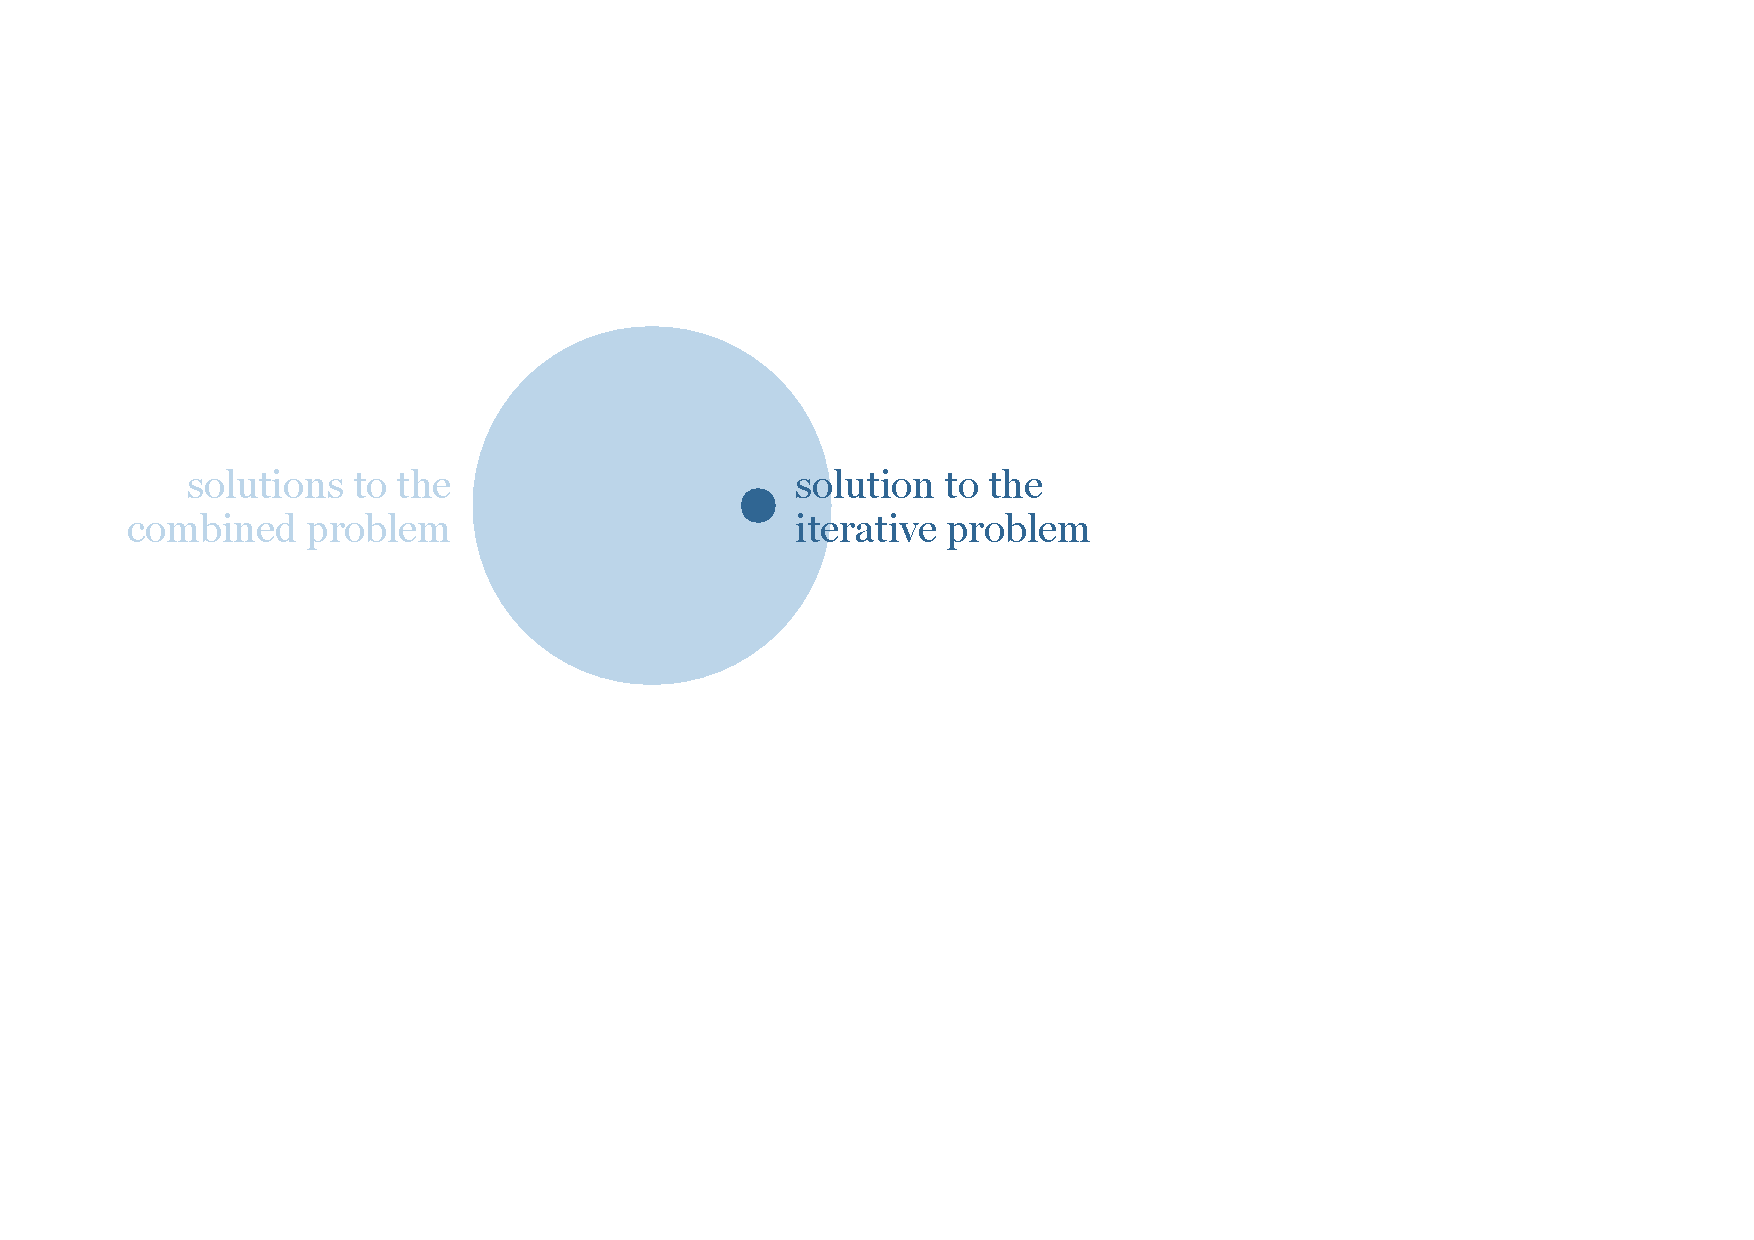
\includegraphics[width=0.8\textwidth]{./images/pca/venn.pdf}
\end{figure}
%\vspace{-1em}

%<figure class="narrow centering">
%<img src="/images/pca/venn.svg"/>
%</figure>

We can say more about this later, but for now we will equate the iterative solution with PCA: the \(\rc{\mbW}\) which not only minimizes the reconstruction error as a whole, but also each column of \(\rc{\mbW}\) minimizes the reconstruction error in isolation, constrained to the subspace orthogonal to the preceding columns. The combined problem does not give us the principal components.

Using the iterative approach, and solving it by projective gradient descent, we can have a look at what the other principal components look like. Let's start with our income data, and derive the second principal component.

\begin{figure}[H]
	\centering
	\includesvg[width=1\textwidth]{./images/pca/sol-w2.svg}
\end{figure}

This is a bit of an open door: in two dimensions, there is only one direction orthogonal to the first principal component. Still, plotting both components like this gives some indication of what the second component is doing. The first component captures the main difference between the people in our dataset: roughly their monthly salary. The second component captures whatever is left; all the noise we introduced like end of year bonuses and alternative sources of income.

Note how PCA reconstructs the original data points. Given the components \(\rc{\mbw_1}, \ldots, \rc{\mbw_k}\), we represent each \(\mbx\) as a weighted sum over these vectors where the latent features \(z_\rc{1}, \ldots, z_\rc{k}\) are the weights:

\[
\mbx' = z_\rc{1}\rc{\mbw_1} + z_\rc{2}\rc{\mbw_2}  + \ldots + z_\rc{k}\rc{\mbw_k}
\]

\begin{figure}[tb]
	\centering
	\includesvg[width=1\textwidth]{./images/pca/wsum.svg}
	\caption*{Reconstruction by principal components in the case where \(\rc{k}=3\). Each latent variable \(z_\rc{r}\) tells us how much of the \(\rc{r}\)-th principal component to add to our reconstruction.}
\end{figure}
%
%<figure class="narrow centering">
%<img src="/images/pca/wsum.svg"/>
%</figure>
%
That's it for the income dataset. We've reached \(\rc{k} = \bc{m}\), so we can go no further.

Let's turn to the dataset of faces, where there are many more principal components to explore.

If we compute the first 30 principal components, we get the following reconstructions.


\begin{figure}[H]
	\centerline{
	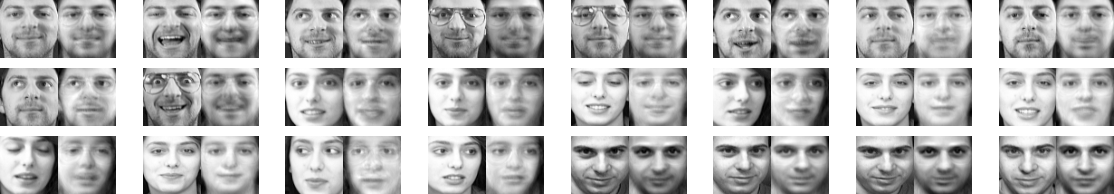
\includegraphics[width=1.2\textwidth]{./images/pca/face-reconstructions-k5.png}
	}
	
\end{figure}
%<figure class="wide">
%<img src="/images/pca/face-reconstructions-k5.png"/>
%</figure>

You can still tell the originals from the reconstructions, but many of the salient features now survive the compression process: the direction of the gaze, the main proportions of the face, the basic lighting, and so on. By looking at the first five principal components, we can see how this is done.

\begin{figure}[H]
	\centerline{
	\includesvg[width=1.2\textwidth]{./images/pca/five-pcs.svg}
	}
\end{figure}
%<figure class="narrow centering">
%<img src="/images/pca/five-pcs.svg"/>
%</figure>

The first one we've seen already. It's flipped around, this time, with the blues and reds reversed, but it defines the same line in space. Note that the magnitude of the higher PCs is much lower: the first principal component does most of the work of putting the image in the right region of space, and the more PCs we add, the more they fine-tune the details. 

The second PC captures mostly lighting information. Adding it to a picture adds to the left side of the image, and subtracts from the right side. We can see this by applying it to some faces from the data.

\begin{figure}[H]
	\centerline{
	\includesvg[width=1.2\textwidth]{./images/pca/int-data-faces-pc1.svg}
	}
\end{figure}
%<figure class="wide-margin">
%<img src="/images/pca/int-data-faces-pc1.svg"/>
%</figure>

The third PC does the same thing, but for top-to-bottom lighting changes. The fourth is a bit more subtle. It's quite challenging to tell from the plot above what the effect is. Here's what we see when we apply it to some faces.

\begin{figure}[H]
	\centerline{
	\includesvg[width=1.2\textwidth]{./images/pca/int-data-faces-pc3.svg}
	}
\end{figure}
%<figure class="wide-margin">
%<img src="/images/pca/int-data-faces-pc3.svg"/>
%</figure>

The PC seems to capture a lot of the facial features we associate with gender. The faces on the left look decidedly more "female", and the faces on the right more male. It's a far cry from the face manipulation methods that are currently popular, but considering that we have only 400 examples, we are only allowed a linear transformation, and that the method originated in 1901 \citep{pearson1901liii}, it's not bad.

\section{Applications of PCA}

Before we finish up, let's look at two examples of how PCA is used in research.
 
\noindent Let's start with a problem which crops up often in the study of fossils and other bones. A trained anatomist can look at, say, a shoulder bone fossil, and tell instantly whether it belongs to a chimpanzee (which is not very rare) or an early ancestor of humans (which is extremely rare). Unfortunately such judgements are usually based on a kind of unconscious instinct, shaped by years of experience, which makes it hard to back it up scientifically. "This is is Hominid fossil, because it looks like one to me," isn't a very rigorous argument. 

PCA is often used to turn such a snap judgement into a more rigorous analysis. We take a bunch of bones that are entirely indistinguishable to the layperson, and we measure a bunch of \bc{features}, like the distances between various parts on the bone. We then apply PCA and plot the first two principal components.

Here is what such a scatterplot looks like for a collection of scapulae (shoulder bones) of various great apes and hominids.

\begin{figure}[H]
	\centerline{
	\includesvg[width=1\textwidth]{./images/pca/bones.svg}
	}
\end{figure}

%<figure class="narrow">
%<img src="/images/pca/bones.svg"/>
%<figcaption>Reproduced from [4].</figcaption>
%</figure>

This particular figure is from \citet{young2015fossil} (reproduced with permission) which is \href{https://www.pnas.org/content/112/38/11829}{available online}, but the literature is full of images like these. Here, the authors took scans of about 350 scapulae. We can clearly see different species forming separate clusters. If we find a new scapula, we can simply measure it, project it to the first two principal components, and show that it ends up among the Homo Ergaster to prove that our find is special. What's more, not only can we tell the Hominin fossils apart, we see that they seem to lie on a straight line from chimpanzees to modern humans, giving a clue as to how human evolution progressed.

\begin{aside}%
This analysis is based on full 3D scans of the bones, but it also works if you measure a number of features by hand.
\end{aside}

Let's add one final example, to really hammer home the magic of PCA. When large-scale genome databases began to be gathered, one of the first things researchers did, was to perform principal component analyses. 

All you need to do is to extract some features from each DNA sequence. For instance, you can identify a few hundred thousand important genetic markers, and use the presence or absence of each as a binary feature.

\enlargethispage{3em}

\begin{figure}[H]
	\centerline{
	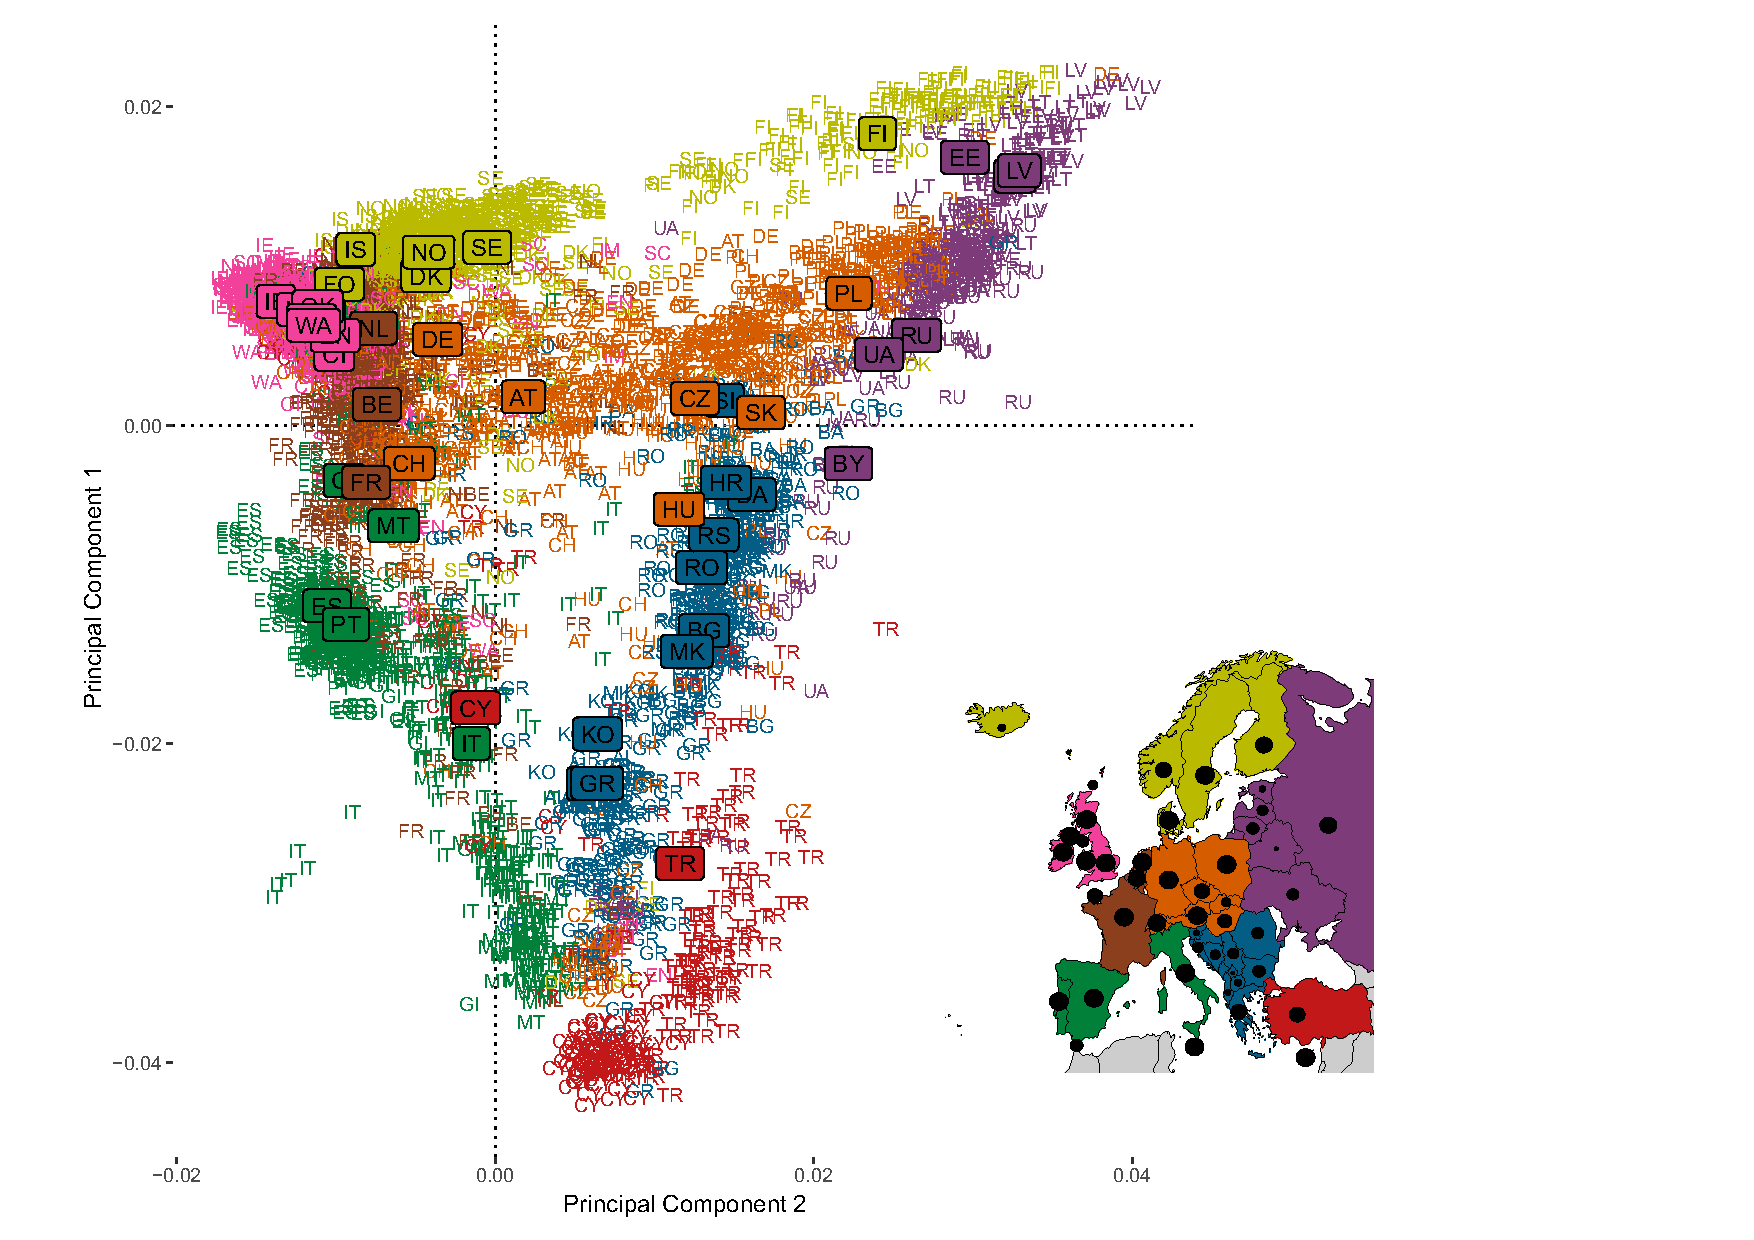
\includegraphics[width=0.7\textwidth]{./images/pca/europe-pnas.pdf}
	}
	\caption*{A PCA analysis of a European population, similar to the one by \cite{novembre2008genes}, colored by ancestry. Adapted from \cite{gilbert2022revealing}.
	}
\end{figure}

PCA has been used this way in genetics for a long time, but it wasn't until large datasets, annotated with country of origin, became available, that a peculiar pattern was noticed. 

This pattern was first found by \citet{novembre2008genes}, using a dataset of 1\,387 Europeans, measuring about 200\,000 genetic markers. They applied PCA, and plotted the first two principal components. They then colored the instances by the person's ancestral country of origin (the country of origin of the grandparents if available, otherwise the person's own country of origin). What they saw was something like a blurry picture of Europe.

%  applied PCA to a database of 1387 European DNA sequences. For each instance, they measured about half a million sites on the DNA sequences to use as features. This is similar to the face example: many more features than instances.

%The authors applied PCA, and plotted the first two principal components. They colored the instances by the person's ancestral country of origin (the country of origin of the grandparents if available, otherwise the person's own country of origin). Here is what they saw.

%\begin{figure}[H]
%	\centerline{
%	\includesvg[width=0.9\textwidth]{./images/pca/europe.svg}
%	}
%\end{figure}

%<figure class="narrow">
%<img src="/images/pca/europe.svg"/>
%<figcaption>Reproduced from [5].</figcaption>
%</figure>

The first principal component corresponds roughly to how far north the person lives (or their ancestors did) and the second principal component to how far east they live. This means that a scatterplot shows up as a fuzzy map of Europe. If we sent a thousand DNA samples off to aliens on the other side of the galaxy, they could work out a rough image of the geography of Earth.

\begin{aside}%
Note that while this result is impressive, it's easy to misinterpret what this means. These two principal components together explain no more than a few percent of the variance. That is, while we can make a crude prediction of a person's origin from their DNA, we can predict almost nothing about their DNA from their origin. We saw something similar in the example of the Olivetti data: we could predict people's gender and age from the first few principal components, but when we reconstructed the photograph from just this information, the result removed almost all relevant details about the subject of the photograph.
\end{aside}


Wrapping up, what have we learned so far? We have defined PCA as an iterative optimization problem designed to compress high dimensional data into fewer dimensions, and to minimize the resulting reconstruction loss. We've shown one simple way to find this solution, a laborious and inaccurate way, but enough to get the basic idea across. We then looked at various practical uses of PCA: analyzing human faces, human fossils, and human DNA. We showed that in many cases, PCA magically teases out high-level semantic features hidden in the data: the species of the fossil, the location of the subject in Europe, or the subject's age.

What we haven't discussed fully, is where this magical property comes from. We've shown that it isn't \emph{just} the compression objective, since optimizing just that in one single optimization doesn't lead to the PCA solution. Among the set of all solutions that minimize the reconstruction error, the PCA solution takes a special place. Why that's the case, and why it this should emerge form optimizing the principal components one by one, greedily if you will, instead of all together, we will discuss in the next chapter. To do so, we'll need to dig into the subject of \emph{eigenvectors}, the underlying force behind almost everything that is magical about linear algebra.


%\pagebreak
%%\pagestyle{empty}
%~
%\thispagestyle{empty}
%\pagebreak 
\cleardoublepage

\chapter{Eigenvectors and eigenvalues}
\pagestyle{fancy}
\label{chapter:eigenvectors}

In the first chapter, we took what I think is the most intuitive route to defining PCA: framing the method in terms of \emph{reconstruction error}. The solution method we used wasn't very efficient or stable, and some parts of the ``why'' question were left unresolved, but we answered the ``how'' question well enough to show the method in action and hopefully convince you that it's worth digging a little deeper.

We'll start by tying up one of the loose ends from the last chapter. There, we defined PCA in terms of reconstruction error, but most other explanations instead  define it in terms of \textbf{variance maximization}. 

I started with the reconstruction error, since it requires fewer assumptions, and the required assumptions feel more intuitive. However, to explain the details of what happens under the hood, the variance perspective is more helpful, so we'll start by adding that to our toolbelt.

\section[Min. reconstruction is max. variance]{Minimal reconstruction error is maximal variance}

In the previous chapter, we defined PCA as a solution to the following problem: for a mean-centered set of instances \(\mbx_\gc{i}\) find a sequence of \(\rc{k}\)  unit vectors \(\rc{\mbw_1}, \ldots, \rc{\mbw_k}\) where each unit vector is defined by

\[
\;\;\;\;\;\;\;\; \rc{\mbw_r} = 
\begin{cases} 
	&\argmax{\rc{\mbw}} \sum_\gc{i} \|\mbx_\gc{i}^T\rc{\mbw}\rc{\mbw} - \mbx_\gc{i}\|^2 \\
	&\;\;\;\;\;\;\text{such that } \rc{\mbw}^T\rc{\mbw} = 1 \hfill \hspace{2em}\bc{\text{(a)}}\\
	&\;\;\;\;\;\;\text{and } \rc{\mbw}^T\rc{\mbw_j} = 0 \text{ for } \rc{j} \in [1 \ldots \rc{r}-1] \hfill \hspace{2em}\bc{\text{(b)}}
\end{cases}
\]

That is, each unit vector defines an approximation of \(\mbx_\gc{i}\), and the objective is to keep the distance between the reconstruction and the original instance as small as possible, while ensuring that \bc{(a)} the vector is a unit vector, and \bc{(b)} the vector is orthogonal to all preceding vectors.

The variance maximization objective takes the same form, but instead of minimizing the reconstruction error, it chooses \(\rc{\mbw}\) to \emph{maximize} the variance of the data projected onto \(\rc{\mbw}\). 

As in the previous chapter, we'll start with the one-dimensional case. We will choose a single unit vector \(\rc{\mbw}\) and project the data onto it orthogonally. That means that for every instance \(\mbx_\gc{i}\), we get a single number \(z_\gc{i}\) which is defined by \(\mbx_\gc{i}^T\rc{\mbw}\).
 
This time, our objective is to choose \(\rc{\mbw}\) so that the variance among the set of \(z_\gc{i}\) is maximized. That means that in this image
\vspace{-0.1em}
\begin{figure}[H]
	\centerline{
	\includesvg[width=0.8\textwidth]{./images/pca/random-w.svg}
	}
\end{figure}
\vspace{-1em}
%<figure class="narrow">
%<img src="/images/pca/random-w.svg" />
%</figure>
\noindent we want to choose \(\rc{\mbw}\) so that the red points are spread out as widely as possible.

Why is this the same as choosing the \(\rc{\mbw}\) that minimizes the reconstruction error? It's easy to see this if we draw a a diagram for a single instance.

\begin{figure}[H]
	\centerline{
	\includesvg[width=1\textwidth]{./images/pca/recvar-diagram.svg}
	}
\end{figure}

%<figure class="narrow">
%<img src="/images/pca/recvar-diagram.svg" />
%</figure>

Note that \(\rc{\mbw}\) is a unit vector, so for the length of the bottom edge of the triangle we have  \(\|\mbx'_\gc{i}\| = \|\rc{\mbw}z_\gc{i}\| = z_\gc{i}\).


By the Pythagoras, \(\|\mbx_\gc{i}\|^2 = \|\bc{\mbr}\|^2 + {z_\gc{i}}^2\). The vector \(\mbx_\gc{i}\) remains constant, since that is given by the data. The only thing we change is the direction of the vector \(\rc{\mbw}\). If we change that to decrease the reconstruction error \(\|\bc{\mbr}\|\), the distance \(z_\gc{i}\) must decrease. The sum of the squares of all \(\mbz_\gc{i}\)'s is the variance of the data.

%\begin{aside}
%I first learned about the equivalence between variance maximization and reconstruction error minimization from  by <a href="http://alexhwilliams.info/">Alex Williams</a>, which uses a similar diagram.
%\end{aside}

Thus, the first principal component is the vector \(\rc{\mbw}\) for which the data has maximum variance when projected onto \(\rc{\mbw}\). For the sake of completeness, let's work this into a proper proof. There's some technical stuff coming up, so we had better get into a more formal mindset.

\begin{theorem}[Equivalence of error and variance optimization.]
The vector \(\rc{\mbw}\) that minimizes the reconstruction error among the reconstructed instances \(\mbx'_\gc{i}\), maximizes the variance among the projections \(z_\gc{i}\).
\end{theorem}
\begin{proof}
The maximal variance objective can be stated as

\begin{align*}
&\argmax{\rc{\mbw}}\; \kc{\frac{1}{n}} \sum_\gc{i} (\bar z - z_\gc{i})^2 \p
\end{align*}

The objective inside the argmax is simply the definition of variance. We can drop the constant multiplier \(\kc{1/n}\), since it doesn't affect where the maximum is. We can show that \(\bar z\), the mean of the projections is 0:
\[
\bar z = \kc{\frac{1}{n}}\sum_\gc{i} \rc{\mbw}^T\mbx_\gc{i} = \rc{\mbw}^T\left( \kc{\frac{1}{n}} \sum_\gc{i} \mbx_\gc{i}\right) = \rc{\mbw}^T \mathbf{0} \p
\]

\begin{aside}The last step follows from the assumption that the data is mean-centered.\end{aside}


Thus our objective simplifies to

\begin{align*}
&\argmax{\rc{\mbw}} \sum_\gc{i} {\mbz_\gc{i}}^2 \p
\end{align*}

From our diagram above, we know that \(\|\mbx_\gc{i}\|^2 = \|\bc{\mbr}\|^2 + z_\gc{i}^2\), or, equivalently

\begin{align*}
\|\mbx_\gc{i}\|^2 &= \|\bc{\mbx_\gc{i} - \mbx'_\gc{i}}\|^2 + z_\gc{i}^2 \\
z_\gc{i}^2 &= \|\mbx_\gc{i}\|^2 - \|\bc{\mbx_\gc{i} - \mbx'_{\gc{i}}}\|^2 \p
\end{align*}

Filling this in to the optimization objective, we get

\begin{align*}
&\argmax{\rc{\mbw}} \sum_\gc{i} \kc{||\mbx_i||^2} \oc{-} ||\mbx_\gc{i} - \mbx_\gc{i}'||^2 \p
\end{align*}

where \(\kc{\|\mbx_i\|^2}\) is a constant we can remove without affecting the maximum and removing \oc{the minus} turns the maximum into a minimum. Thus, we end up with 

\begin{align*}
&\argmin{\rc{\mbw}} \sum_\gc{i} ||\mbx_\gc{i} - \mbx'_\gc{i}||^2
\end{align*}

which is the objective for minimizing the reconstruction loss. \hfill\qed

\end{proof}

The rest of the procedure is the same as before. Once we've chosen \(\rc{\mbw_1}\) to maximize the variance, we choose \(\rc{\mbw_2}\) to maximize the variance and to be orthogonal to \(\rc{\mbw_1}\), we choose \(\rc{\mbw_3}\) to maximize the variance and to be orthogonal to  \(\rc{\mbw_1}\) and to  \(\rc{\mbw_2}\) and so on.

In the previous chapter, we also defined a \textbf{combined problem}, which combined all the vectors together in one optimization objective. We can work out an equivalent for the variance perspective (the proof is in Section~\ref{section:ch2-app} of the appendix). 

\begin{theorem}[Equivalence of combined optimization.] The combined problem for reconstruction error minimization.
\begin{align*}
&\argmin{\rc{\mbW}} \sum_\gc{i} \|\mbx_\gc{i} - \mbx'_\gc{i}\|\\
&\;\;\;\text{such that } \rc{\mbW}^T\rc{\mbW} = \mbI\\
\end{align*}
is equivalent to the following variance maximization problem
\begin{align*}
&\argmax{\rc{\mbW}} \sum_{\gc{i}, \rc{r}} {z_{\gc{i}\rc{r}}}^2 \;\;\;\;\;\text{with } z_{\gc{i}\rc{r}} = \rc{\mbw_r}^T\mbx_\gc{i}\\
&\;\;\;\text{such that } \rc{\mbW}^T\rc{\mbW} = \mbI \p\\
\end{align*}
\end{theorem}

If we want to optimize a matrix \(\rc{\mbW}\) with mutually orthogonal unit vectors for columns in one go, then maximizing the sum of the variances in all \rc{latent directions} is equivalent to minimizing the reconstruction loss defined in the combined approach  

One consequence is that since \(\rc{\mbW} = \mbI\) was a solution of the error minimization problem (with \(\rc{k} = \bc{m}\)) it must be a solution for the variance maximization problem as well. 

\index{Variance!maximization}

This tells us something interesting. If we set \(\rc{\mbW} = \mbI\), then \(\sum_{\gc{i}, \rc{r}} {z_{\gc{i}\rc{r}}}^2\) is just the sum of all the variances of all the features in our data. For all solutions at \(\rc{k} = \bc{m}\), this must be the total variance among the latent features. For solutions to the problem at some \(\rc{k} < \bc{m}\) the variance is less than or equal to this value. Each principal component adds a little variance to the total sum of variance, and when we have enough principal components to reconstruct the data perfectly, the sum of the variances along the principal components equals the sum total variance in the data.

Here's what that looks like for the Olivetti faces data. 

\begin{figure}[H]
	\centerline{
	\includesvg[width=1\textwidth]{./images/pca/sum-variance.svg}
	}
\end{figure}

%<figure class="narrow">
%<img src="/images/pca/sum-variance.svg" />
%</figure>

We plot the sum total of the variances of the data as a \gc{green vertical line} and the sum total of the PCA solution for increasing \(\rc{k}\) as a red line.

\index{Variance!sum of}

\begin{aside}In this case, we have data that is wider than it is tall, so we reach the ceiling before \(\rc{k} = \bc{m}\), when \(\rc{k}=\gc{n}\). This is to do with the \emph{rank} of the matrix \(\mbX\). We'll shed some light on this in Chapter~\ref{chapter:svd}.
\end{aside}

This shows that we can think of the total variance in all directions in the data space as an additive quantity in the data, which we can call its \emph{information content}. The data contains a certain amount of information and the more latent dimensions we allow, the more of that information we retain. 

\index{Information}

\begin{aside}Don't read too much into the word \emph{information} here. It's just a convenient phrase to use. We could relate it to formal notions of information content, like Shannon's, but not without some serious extra work.
\end{aside}

If we keep all the dimensions, we retain all the information. If we start with the first principal component and add components one by one, we add to the total of squared variances in a sum that eventually sums up to the total of squared variances in the data (much like the reconstruction loss eventually goes to zero). Both perspectives---retaining variance and minimizing reconstruction loss---are formalizations of the same principle; that \emph{we want to minimize the amount of information lost in the projection}.


\section{Eigenvectors}

Let's return to this image.

\begin{figure}[H]
	\centerline{
	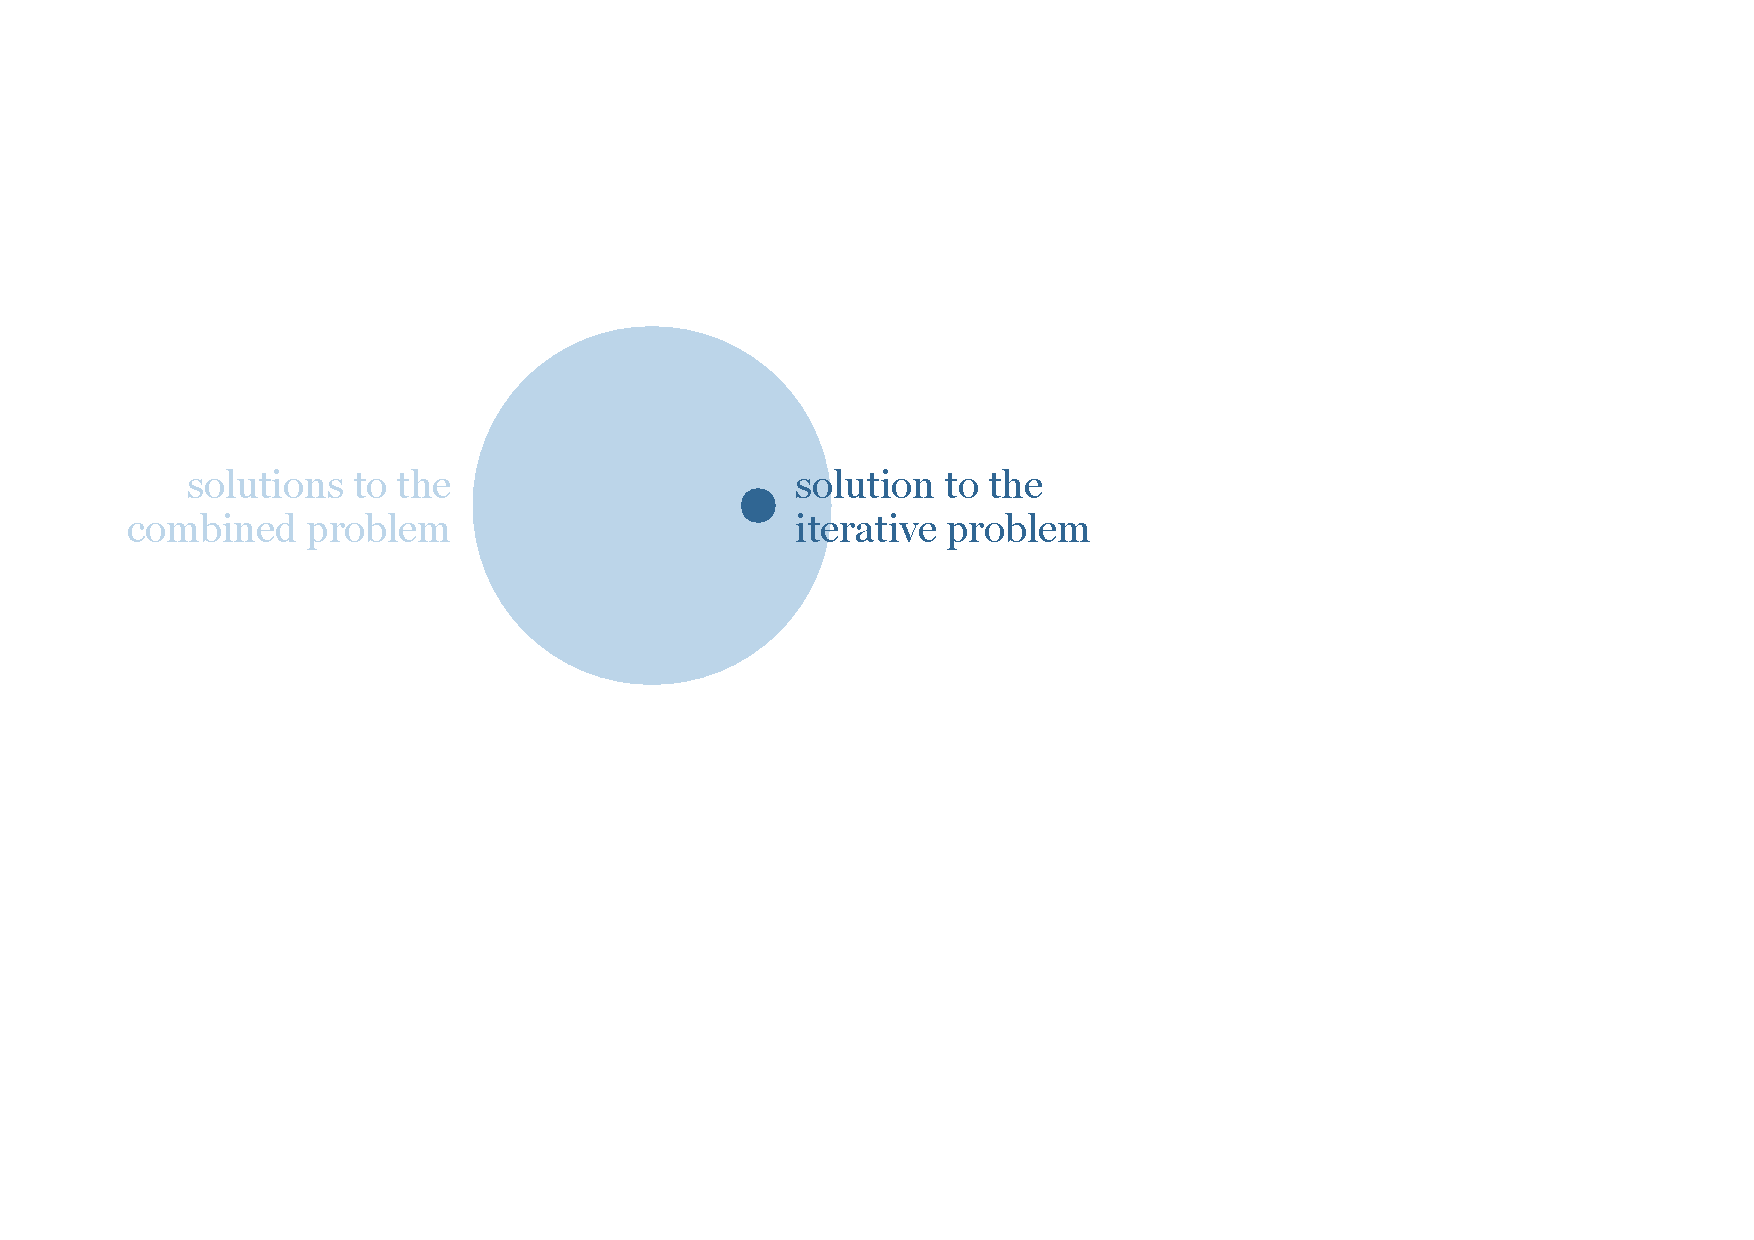
\includegraphics[width=1\textwidth]{./images/pca/venn.pdf}
	}
\end{figure}
%<figure class="narrow">
%<img src="/images/pca/venn.svg" />
%</figure>

These solutions are the same for both perspectives: variance maximization and reconstruction error minimization. We have two unresolved questions about this image.

First, how is it that the solution to the iterative problem (the PCA solution) reaches the same optimum as the solutions to the combined approach? Take a second to consider how strange this is. Solving the iterative problem is a greedy search: once we have chosen \(\rc{\mbw_1}\) we can't ever go back. The process for the combined approach solves all the vectors in sync. How is it that this ability to tune the vectors in concert doesn't give us any advantage in the optimum we find?

The second question, and the question we will answer first, is what is the meaning of the PCA solution among the combined solutions? How can we \emph{characterize} this solution?

The answer to the second question can be summarized in one phrase:

\begin{displayquote}
The principal components are \emph{eigenvectors}.
\end{displayquote}

\index{Eigenvector}

Depending on your background, this will raise one of two questions. \emph{The eigenvectors of what?} or, more simply \emph{What are eigenvectors?} Let's start with the second question, and work our way back to the first.

\subsection{What are eigenvectors?}

The most common, and probably the most intuitive way to think about matrices is \emph{as transformations of points in space}. If we have some vector \(\mbx\) and we multiply it by a matrix \(\bc{\mbA}\), we get a new point \(\mby = \bc{\mbA}\mbx\). If \(\bc{\mbA}\) is square, then \(\mbx\) and \(\mby\) are in the same space. 

\index{Matrix transformations}

A good way to visualize this is by \emph{domain coloring}. We take a large number of points, arranged in a grid, and we color them by some image. This could be a simple color gradient, but we can also choose a photograph or some other image.  Following \href{https://en.wikipedia.org/wiki/Eigenvalues_and_eigenvectors}{Wikipedia's example}, we'll use a picture of the Mona Lisa.

\index{Domain coloring}\index{Mona Lisa}

\begin{figure}[H]
	\centerline{
	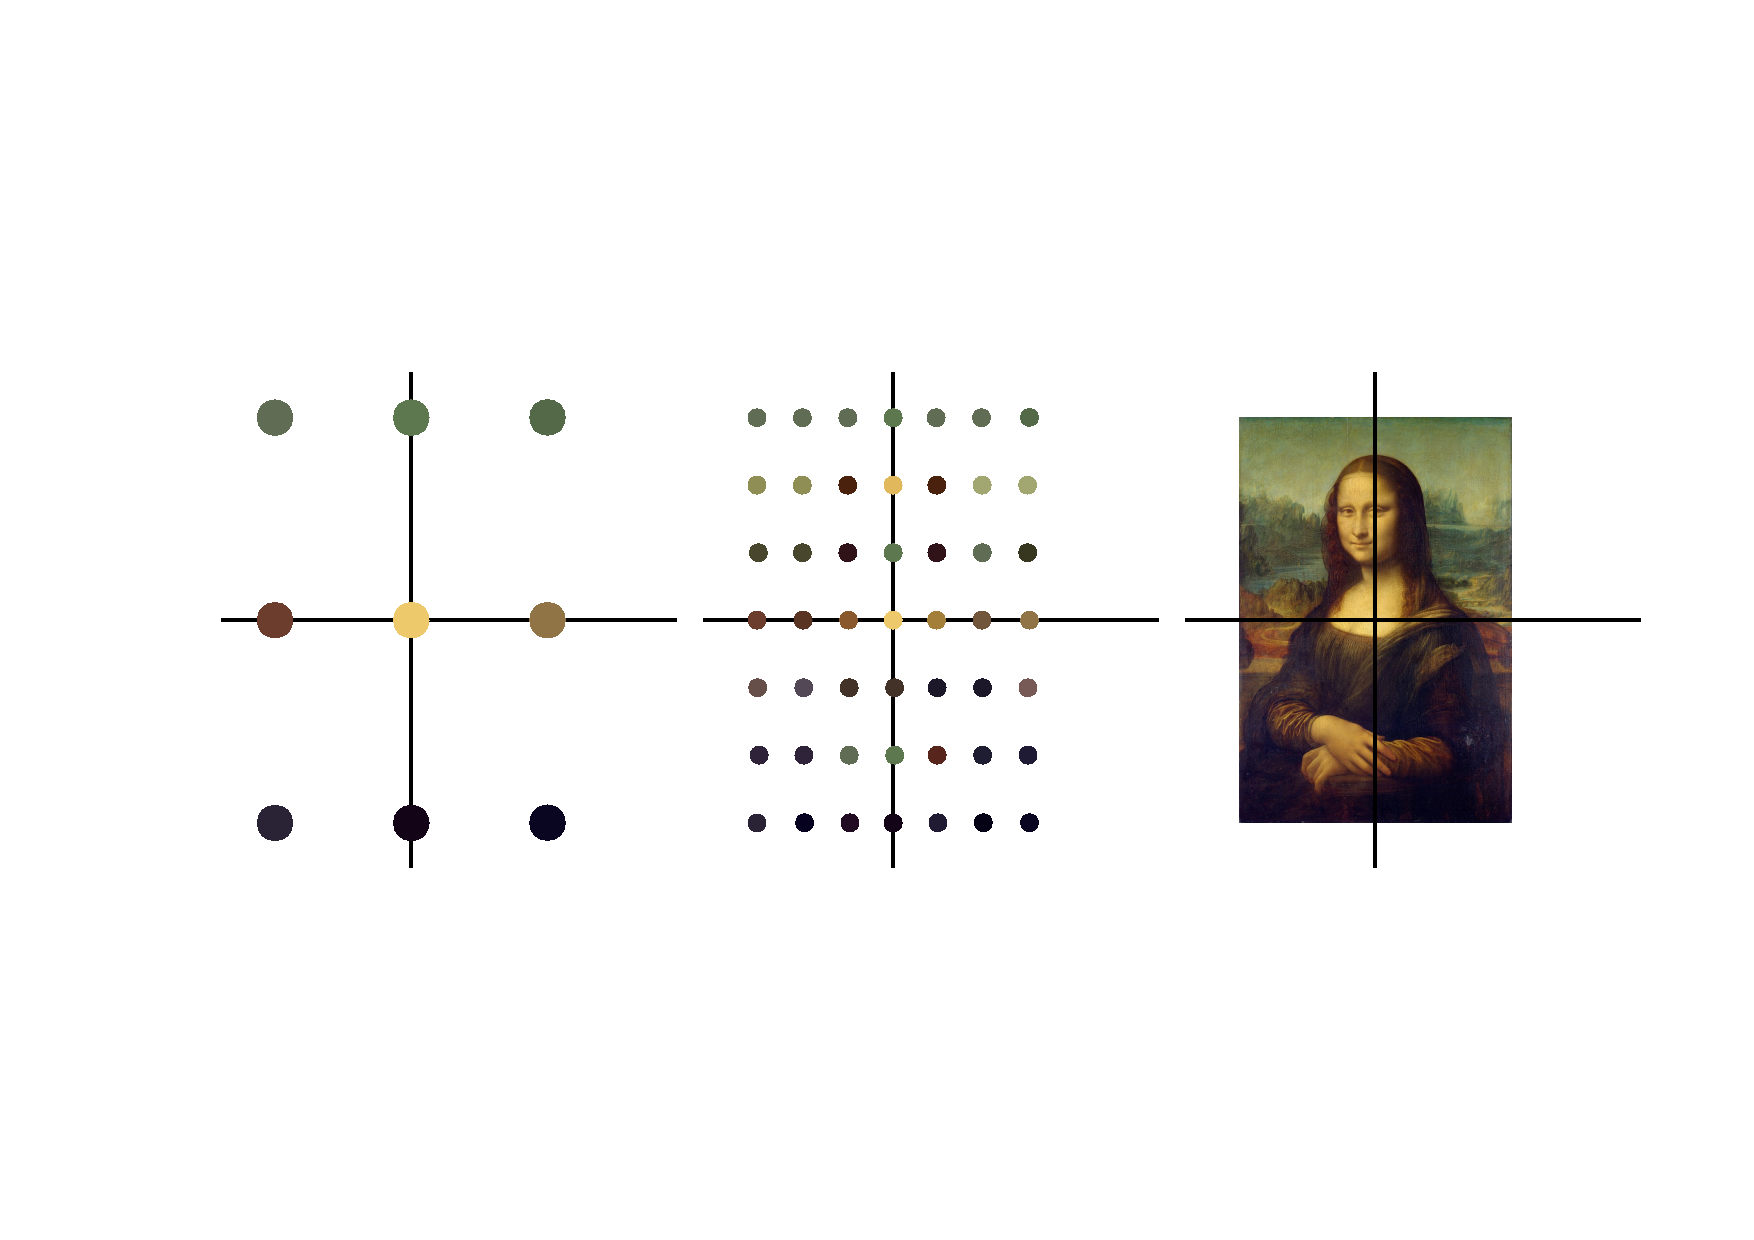
\includegraphics[width=0.7\textwidth]{./images/pca/domain-coloring.pdf}
	}
	\caption*{An increasingly fine-grained domain coloring using the Mona Lisa.}
\end{figure}
%<figure class="narrow">
%<img src="/images/pca/domain-coloring.svg" />
%<figcaption>An increasingly fine-grained domain coloring using the Mona Lisa.</figcaption>
%</figure>

If we apply the transformation \(\bc{\mbA}\) to each of these points, we can tell what effect the matrix has on this space. 

\begin{figure}[H]
	\centerline{
	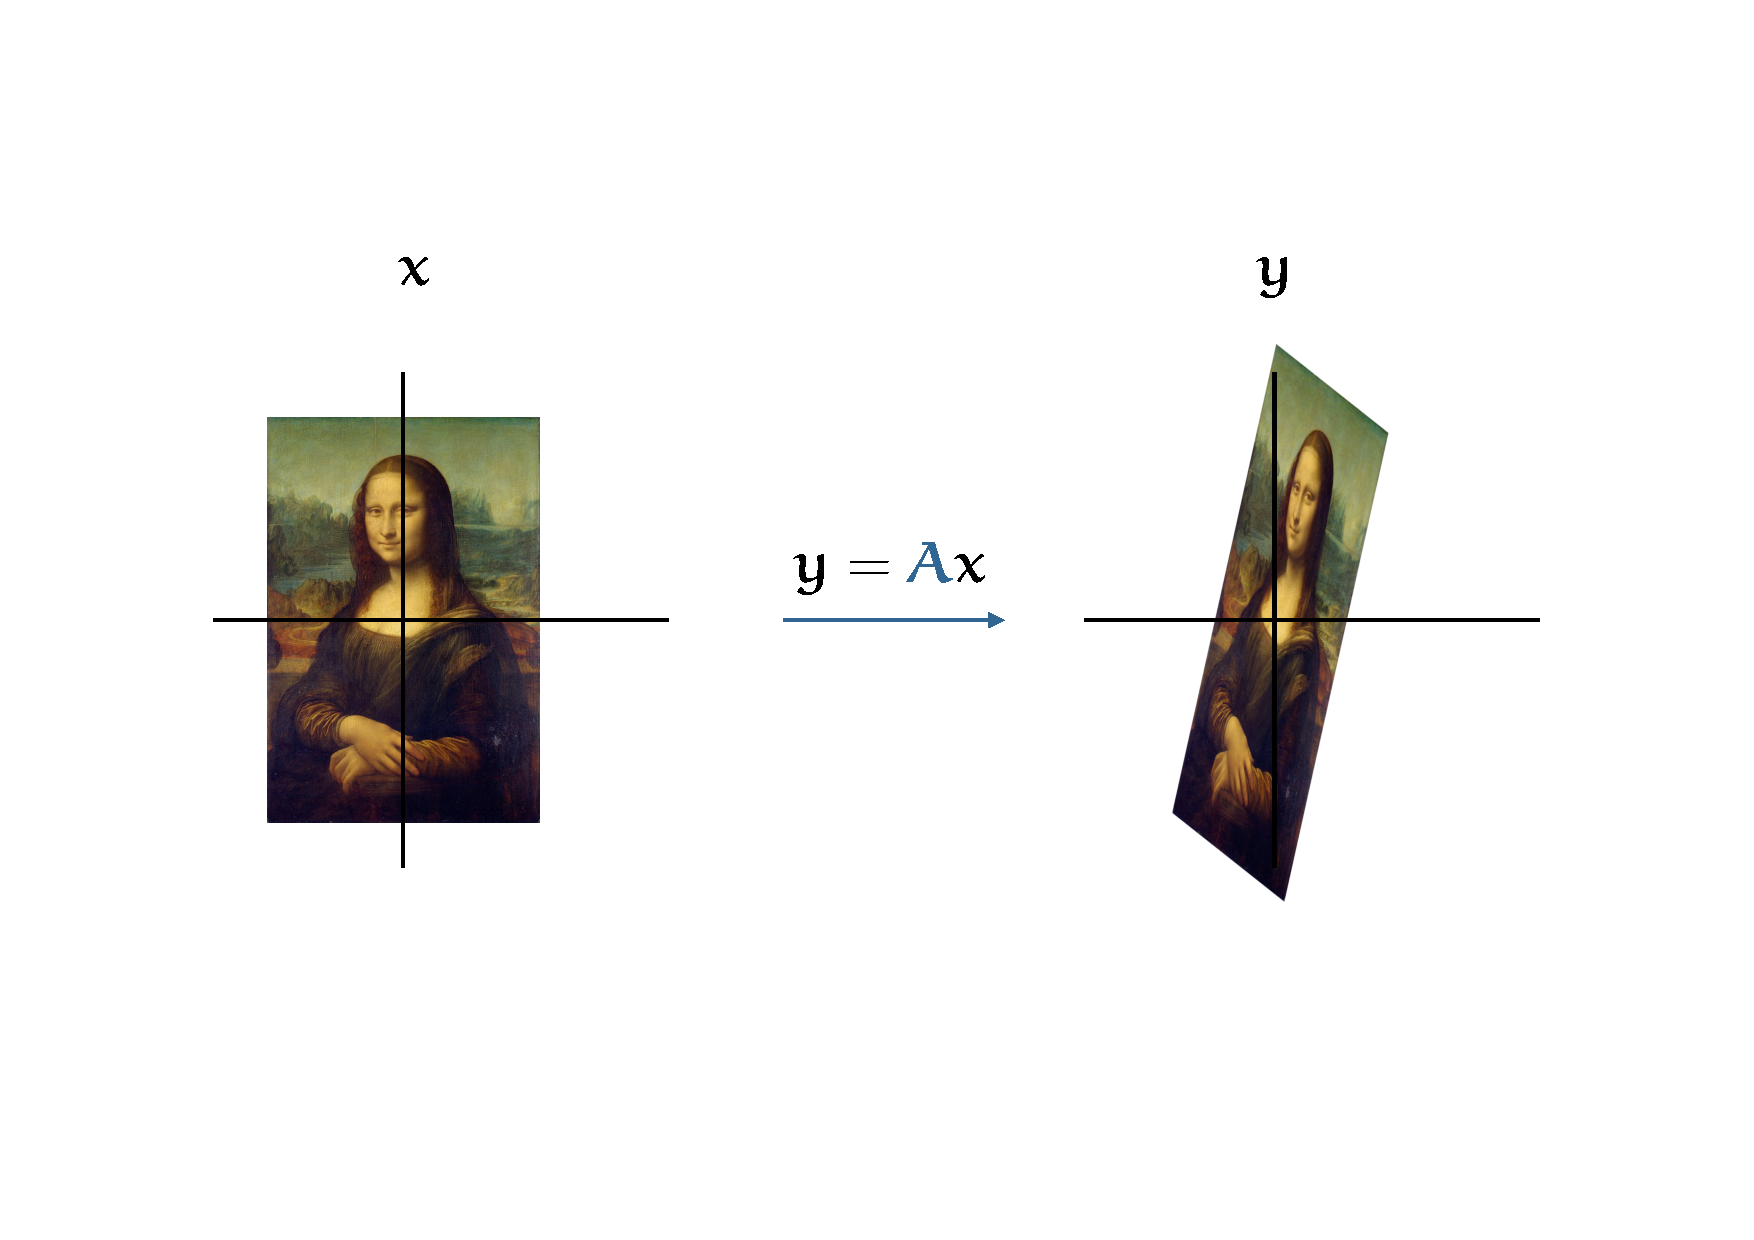
\includegraphics[width=1\textwidth]{./images/pca/basic-transform.pdf}
	}
\end{figure}

%<figure class="narrow">
%<img src="/images/pca/basic-transform.svg" />
%</figure>

All the points are mapped to a new position by \(\bc{\mbA}\) and poor Lisa ends up squished and stretched in various directions. Transformations expressible in a matrix are linear transformations. These are the transformations for which a line in the original image is still a line in the transformed image. This means that we can rotate, stretch, squish and flip the image in any direction we like, but we can't warp, bend or tear it.

In this language of transformation, we can very naturally define what eigenvectors are. The \textbf{eigenvectors of a square matrix \(\bc{\mbA}\)} are defined as those vectors (i.e. points in the image) for which the \emph{direction} doesn't change under transformation  by \(\bc{\mbA}\).

\index{Eigenvector}

It's simplest to see what this looks like for a \emph{diagonal matrix}. For instance in the transformation

\[
\mby = \bc{\begin{pmatrix}2 & 0 \\ 0 & \tfrac{1}{2}\\\end{pmatrix}}\mbx
\]
%
the matrix acts independently on the first and second dimensions, squishing one, and stretching the other.

\begin{figure}[H]
	\centerline{
	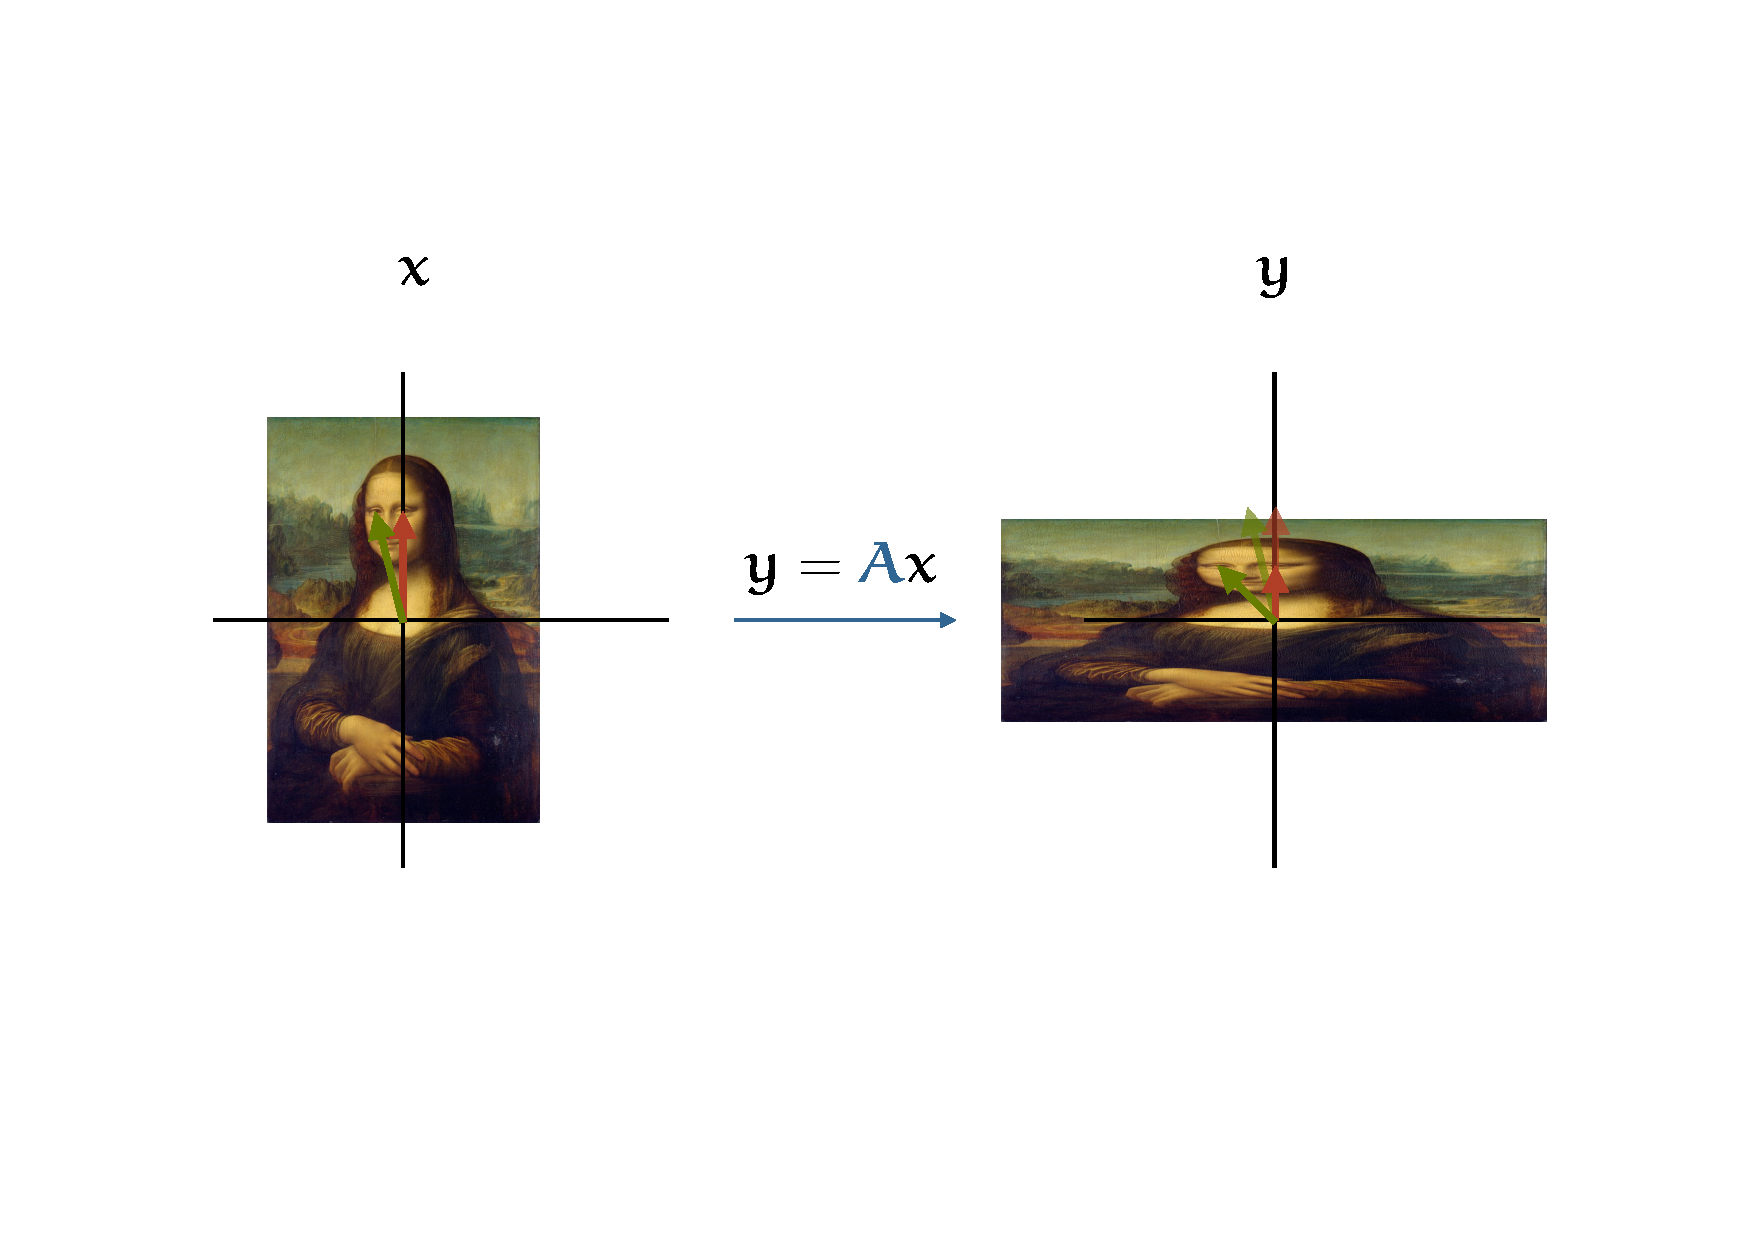
\includegraphics[width=1.2\textwidth]{./images/pca/diagonal.pdf}
	}
\end{figure}

%<figure class="narrow">
%<img src="/images/pca/diagonal.svg" />
%</figure>

In this image we've also drawn two vectors: one \gc{to the middle of Mona Lisa's left eye}, and one \rc{to middle of the right}. Since Leonardo put the right eye dead center in the painting (not by accident, I imagine), the red vector shrinks, but doesn't change direction. The green vector is affected by both the squishing and the stretching, so its direction and magnitude both change. Hence, the red vector is an eigenvector, and the green vector isn't.

In a diagonal matrix, the eigenvectors are always the vectors that point in the same directions as the axes, so they're easy to identify. In general square matrices, finding the eigenvectors is more tricky. 

\index{Eigenvector!of a diagonal matrix}

\begin{aside}See if you can find an eigenvector for the first transformation, shown above. One trick is to start with a random vector, and if it changes direction, transplant it back to the untransformed image and iterate until the vector doesn't change anymore.
\end{aside}

Formally, a vector \(\rc{\mbv}\) is an eigenvector of \(\bc{\mbA}\) if the following holds for some scalar \(\bc{\lambda}\):

\[
\bc{\mbA}\rc{\mbv} = \bc{\lambda}\rc{\mbv} \p
\]

\index{Eigenvector!definition}

This is just a symbolic version of what we said in words above: if \(\rc{\mbv}\) is an eigenvector of \(\bc{\mbA}\), then transforming it changes its magnitude but not its direction, which is the same as saying we can multiply it by a scalar instead of by a matrix. The scalar corresponding to the eigenvector, in this case \(\bc{\lambda}\) is called an \textbf{eigenvalue} of the matrix.

\begin{aside}It's not at all clear from the definition why these vectors should be meaningful or special. For now, just trust me that eigenvectors are worth knowing about.
\end{aside}

To build your intuition, consider for a second the question of whether a pure rotation matrix has eigenvectors (the zero vector doesn't count). It shouldn't take long to convince yourself that a rotation in two dimensions doesn't. At least, not usually. There are two exceptions: rotating by 360 degrees (which is just \(\mbI\)) and rotating by 180 degrees. In both cases, every vector is an eigenvector. In the first with eigenvalue \(\bc{1}\), and  in the second with eigenvalue \(\bc{-1}\). 

\index{Eigenvector!of a rotation matrix}

In three dimensions, rotation is a different story: try pointing straight up in the air and spinning around. The direction of your arm doesn't change as you rotate, so your arm is an eigenvector. Your nose does change direction, so your nose is not an eigenvector.

We saw that when a matrix is diagonal, its eigenvectors are \emph{aligned with the axes}, so they're easy to find. For other matrices, we need to do some more work. One trick is to simply transform the matrix so that the eigenvectors are aligned with the axes, and then to transform it back again.

This is easiest to understand if we work backwards: given some eigenvectors, find the transformation for them.

Here are some vectors drawn on top of the Mona Lisa. What is the transformation for which these vectors do not change direction? 


\begin{figure}[H]
	\centerline{
	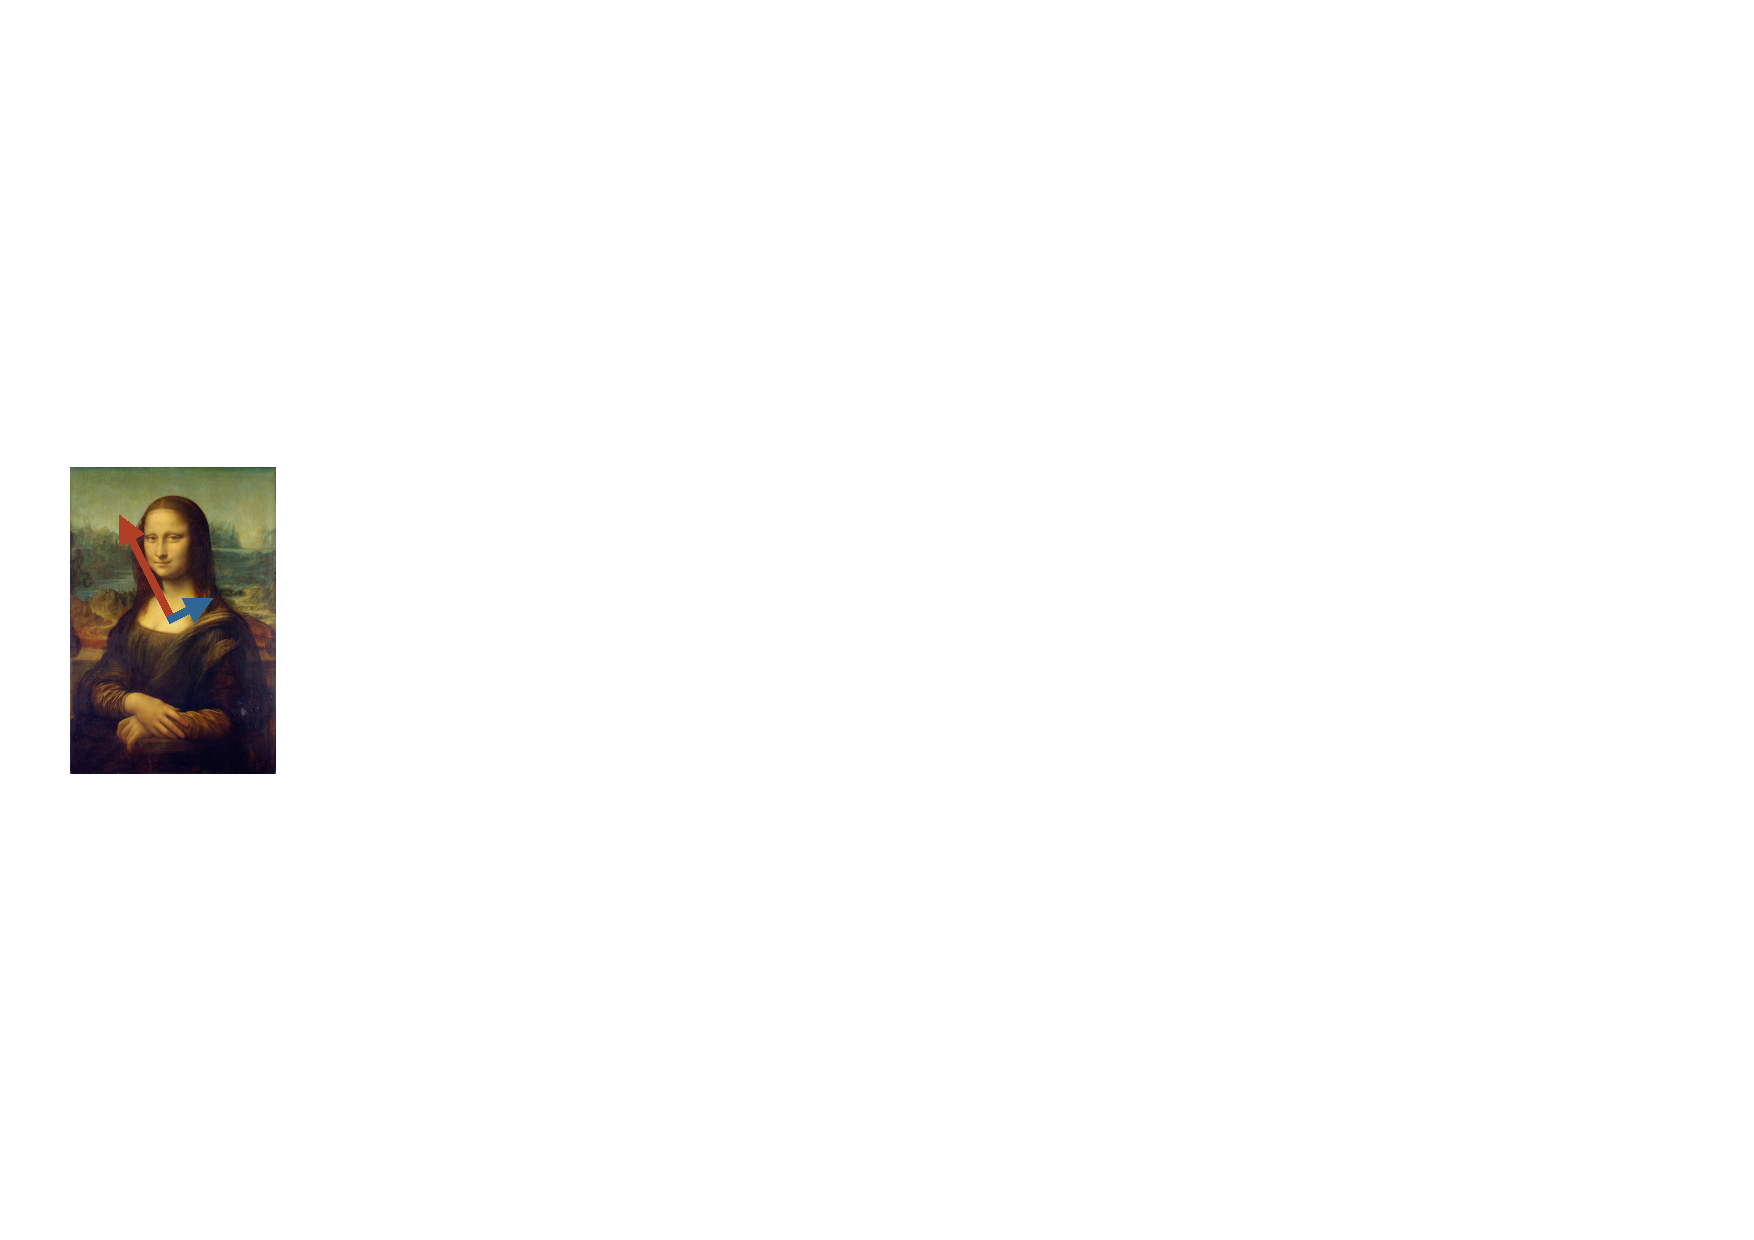
\includegraphics[width=.6\textwidth]{./images/pca/mona-eigen.pdf}
	}
\end{figure}

%<figure class="narrow centering">
%<img src="/images/pca/mona-eigen.svg" class="own-size"/>
%</figure>

We have made things easy for ourselves by making the eigenvectors orthogonal. This means we can \emph{rotate} the image to put the eigenvectors on the axes. We can then do any stretching and squishing we like along the axes, and rotate the image back. 

\begin{figure}[H]
	\centerline{
	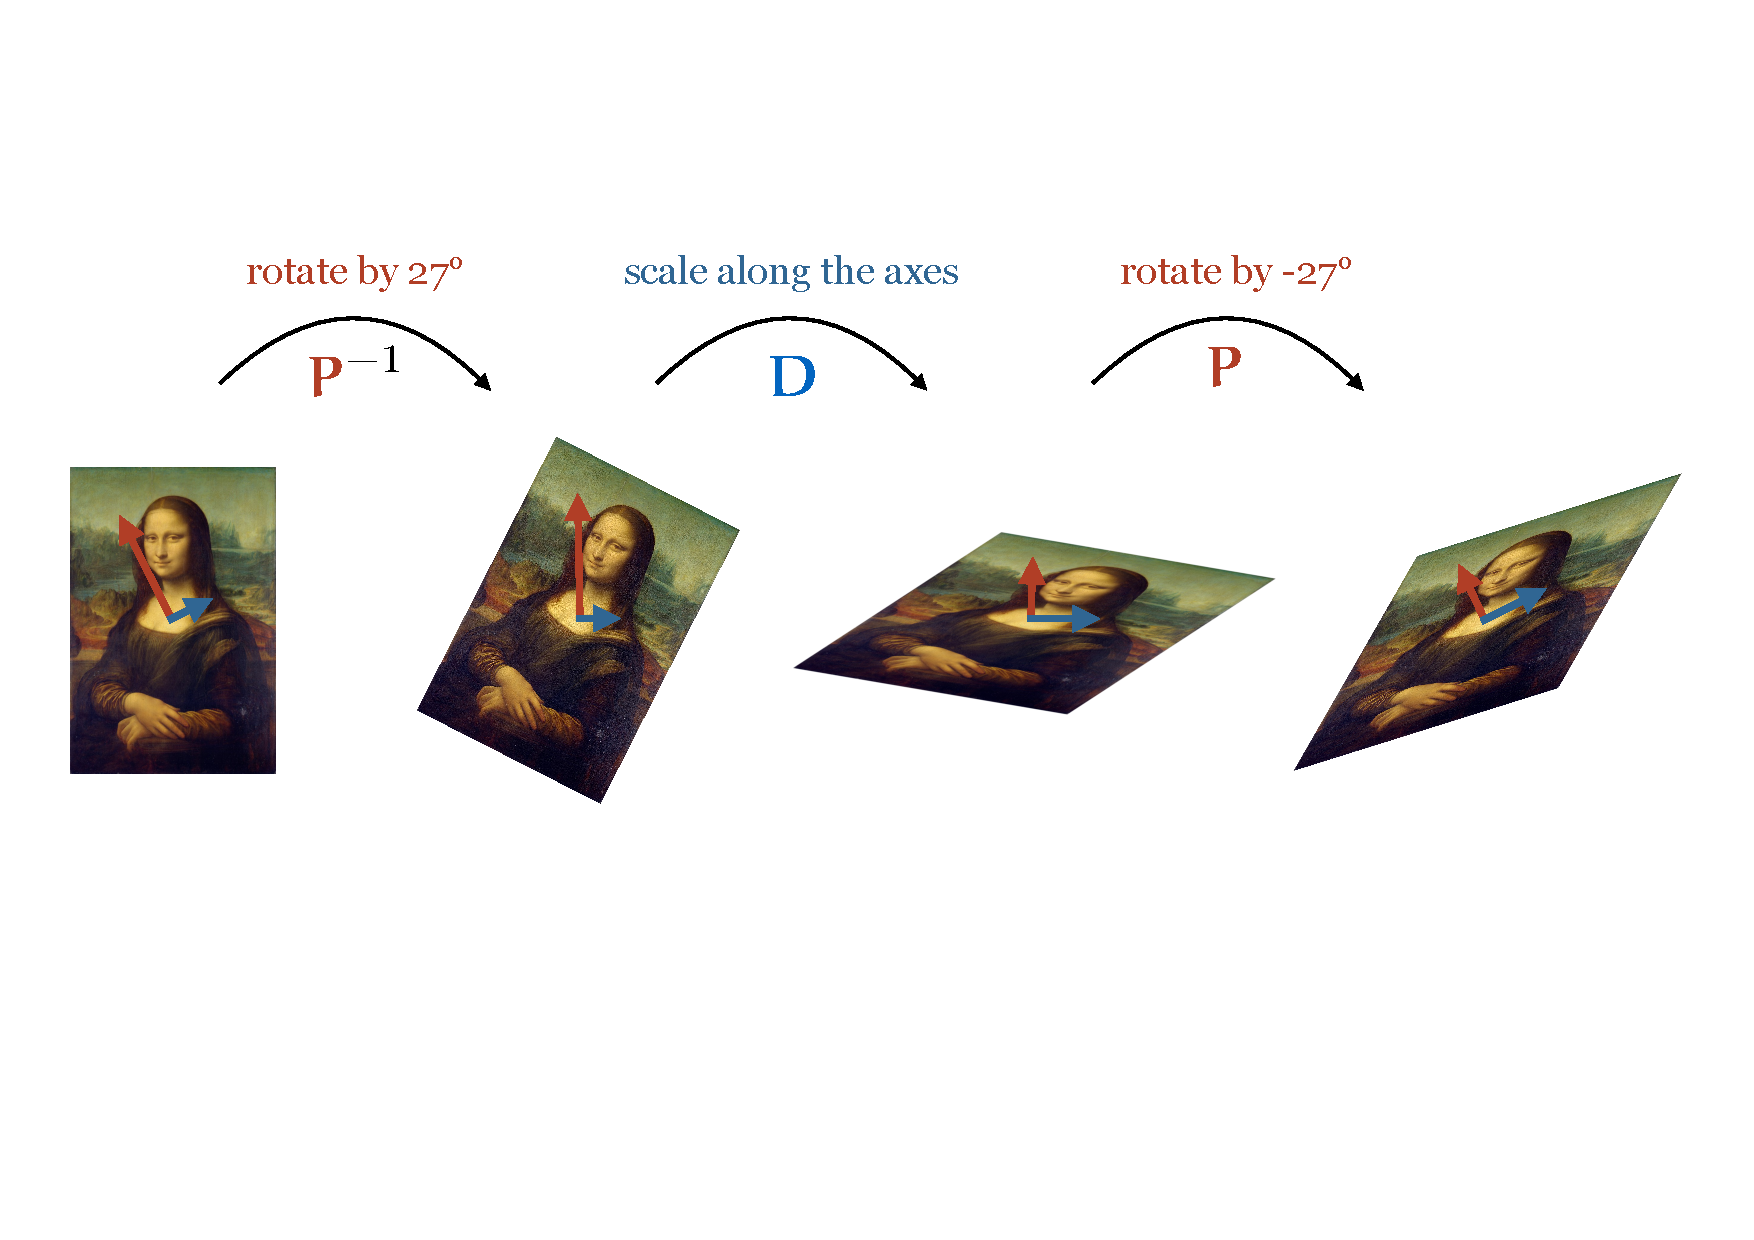
\includegraphics[width=1.2\textwidth]{./images/pca/mona-steps.pdf}
	}
\end{figure}

%<figure class="narrow">
%<img src="/images/pca/mona-steps.svg"/>
%</figure>

Note how, comparing the first and the last image, the red and blue vector change their shape, but not their direction.

Any change we make to the direction of the vectors in the \rc{first step} is reversed exactly in the \rc{last step}: the only permanent change to any \emph{directions} is made in the \bc{middle step}. Therefore, those vectors which don't change direction in the middle step, never change direction at all, and must therefore be eigenvectors. These are the vectors that align with the axes in the middle figure, since the middle transformation is along the axes. Therefore, the vectors which are mapped to align with the axes by the first step are the eigenvectors of the complete transformation \emph{consisting of all three steps}.

All three of these steps can be expressed as matrix transformations. We will call the matrix for the \rc{last step} \(\rc{\mbP}\). The \rc{first step} is then \(\rc{\mbP}^{-1}\), since it needs to undo \(\rc{\mbP}\) exactly. This means that we must require that \(\rc{\mbP}\) is invertible. 

\begin{aside}We could also call the first step \(\rc{\mbP}\) and the last step \(\rc{\mbP}^{-1}\), of course, but it works out more neatly if we call the last step \(\rc{\mbP}\).\end{aside}

In the example, \(\rc{\mbP}\) is a rotation matrix, but the principle generalizes to all invertable matrices. 

We have seen the approach for the middle step already: it is expressed by a diagonal matrix, which we'll call \(\bc{\mbD}\). The composition of these three steps is our transformation matrix \(\bc{\mbA}\). 

\pagebreak

\noindent We compose transformations by multiplying their matrices, so we have:

\[
\bc{\mbA} = \rc{\mbP}\bc{\mbD}\rc{\mbP}^{-1} 
\]

Note that for a transformation \(\bc{\mbA}\mbx = \rc{\mbP}\bc{\mbD}\rc{\mbP}^{-1}\mbx\), the rightmost matrix is applied first, so the direction of the matrices is reversed from the steps in  image above.

Now we can work backwards: For any given matrix \(\bc{\mbA}\), \emph{if} we can decompose it in this way, as the product of some \rc{invertible matrix}, some \bc{diagonal matrix} and the \rc{inverse of the invertable matrix}, then we know three things:

\begin{itemize}
\item The eigenvectors of \(\bc{\mbA}\) are the vectors that are mapped by \(\rc{\mbP}^{-1}\) to align to the axes. Any change of direction introduced by \(\rc{\mbP}^{-1}\) is undone by \(\rc{\mbP}\), so the only vectors whose direction is unchanged are those mapped to the eigenvectors of \(\bc{\mbD}\) (i.e. to the axes).
\item The eigenvectors are also those vectors which to which axis-aligned vectors are transformed by \(\rc{\mbP}\).
\item The eigen\emph{values} of \(\bc{\mbA}\) are the elements along the diagonal of \(\bc{\mbD}\). Any change of magnitude introduced by \(\rc{\mbP}^{-1}\) is undone by \(\rc{\mbP}\), so only the changes made by \(\bc{\mbD}\) remain. An eigenvector mapped to axis \(i\) by \(\rc{\mbP}\) is scaled by \(\bc{D}_{ii}\), which is therefore the corresponding eigenvalue.
\end{itemize}


For a given matrix \(\bc{\mbA}\), finding a diagonal matrix \(\bc{\mbD}\) and an invertible matrix \(\rc{\mbP}\) so that \(\bc{\mbA} = \rc{\mbP}\bc{\mbD}\rc{\mbP}^{-1}\) is called a \textbf{diagonalization} or an \textbf{eigendecomposition} of \(\bc{\mbA}\). 

\index{Diagonalization}\index{Eigendecomposition}

So, given a diagonalization of \(\bc{\mbA}\), which are the eigenvectors? We use the second bullet point above. If we take an axis-aligned vector and transform it by \(\rc{\mbP}\), the result is an eigenvector.

We have one eigenvalue per axis, so we'll look for one eigenvector for each. For the vectors to feed to the transformation, we can just take axis-aligned unit vectors (also known as one-hot vectors). Each will transform to an eigenvector. We can do the transformation for all vectors in one go by concatenating the vectors as the columns of one matrix. For the unit vectors this simply results in the identity matrix \(\mbI\), and for the eigenvectors, this results in a matrix we will call \(\oc{\mbE}\). So we are looking the matrix \(\oc{\mbE}\) for which 


\index{One-hot vector}\index{Axis-aligned vector}

\[
\rc{\mbP}\mbI = \oc{\mbE} \p
\]

Removing \(\mbI\) tells us that the eigenvectors we are looking for are simply the columns of \(\rc{\mbP}\).

\subsection{The spectral theorem}

Note that we were careful above to say \emph{if} \(\bc{\mbA}\) can be diagonalized. Not all square matrices can be diagonalized. A theorem showing if and when a particular class of transformations can be diagonalized is called a \emph{spectral theorem}.

\index{Spectral theorem}

\begin{aside}The set of eigenvalues of a matrix is sometimes called its spectrum, so methods and results using these principles often use the adjective \emph{spectral}. For instance, we have \href{https://en.wikipedia.org/wiki/Spectral\_clustering}{spectral clustering}, \href{https://en.wikipedia.org/wiki/Spectral\_graph_theory}{spectral graph theory} and \href{https://en.wikipedia.org/wiki/Spectral\_method}{spectral ODE solvers}.
\end{aside}

\index{Spectral methods}\index{Spectrum (of a matrix)}

There are many spectral theorems, but we'll only need the simplest. The spectral theorem for \emph{symmetric matrices}. A symmetric matrix is a square matrix \(\bc{\mbA}\) which is symmetric across the diagonal. That is, it has \(\bc{A}_{ij} = \bc{A}_{ji}\), or equivalently \(\bc{\mbA}^T = \bc{\mbA}\). We'll call this \emph{the} spectral theorem in the context of this book.

To state the theorem, we first need to define \textbf{orthogonal matrices}. These are square matrices in which all columns are mutually orthogonal unit vectors. 

\index{Orthogonal matrix}

This should sound familiar, it's the constraint we placed on our principal components in the previous chapter. In the combined problem, the constraint \(\rc{\mbW}^T\rc{\mbW} = \mbI\) is simply a requirement that the matrix \(\rc{\mbW}\) be orthogonal.

Why? Remember that matrix multiplication is just a collection of all dot products of rows on the left with columns on the right, so in this case all columns of \(\rc{\mbW}\) with all other columns of \(\rc{\mbW}\). On the diagonal of \(\rc{\mbW}^T\rc{\mbW}\), we find all dot products of columns of \(\rc{\mbW}\) with themselves, which are all \(1\), because they are all unit vectors. Off the diagonal we find all dot products of all columns with other columns. These are all zero, because they are all mutually orthogonal.

\begin{aside}Geometrically, orthogonal matrices represent those transformations that do not change the magnitude of any vector: that is, rotations and reflections.
\end{aside}

A very useful property of orthogonal matrices is that their inverse is equal to their transpose: \(\rc{\mbW}^{-1} = \rc{\mbW}^T\). This follows directly from the fact that \(\rc{\mbW}^T\rc{\mbW} = \mbI\), because the inverse of \(\rc{\mbW}\) is defined as a matrix \(\rc{\mbW}^{-1}\) such that \(\rc{\mbW}^{-1}\rc{\mbW} = \mbI\).

\index{Orthogonal matrix!inverse of}

This property makes orthogonal matrices especially nice to work with, since we can take the inverse---usually a costly and numerically unstable operation---by flipping the indices around, which we can do in constant time, with no numerical instability. 

We can now state the spectral theorem.

\begin{theorem}[The spectral theorem.] Call a matrix \(\bc{\mbA}\) \emph{orthogonally diagonalizable} if it is diagonalizable  with the additional constraint that \(\rc{\mbP}\) is orthogonal
\[
\bc{\mbA} = \rc{\mbP}\bc{\mbD}\rc{\mbP}^T \p
\]

A matrix \(\bc{\mbA}\) is orthogonally diagonalizable if and only if \(\bc{\mbA}\) is symmetric.
\end{theorem}

\index{Spectral theorem!statement}

Proving this now would require us to discuss too many extra concepts that aren't relevant for this part of the story. On the other hand, this theorem is very much the heart of PCA: everything it is and can do follows from this result. We'll take it at face value for now, and answer the rest of our questions. The next chapter will be entirely dedicated to proving the spectral theorem.

For now, just remember that if we have a square, symmetric matrix, we can diagonalize it with an orthogonal matrix \(\rc{\mbP}\) and a diagonal matrix \(\bc{\mbD}\). The diagonal elements of \(\bc{\mbD}\) will be the eigenvalues and the columns of \(\rc{\mbP}\) will be the corresponding eigenvectors. 

Note that the spectral theorem implies that there are \(\gc{n}\) eigenvalues (since \(\bc{\mbD}\) has \(\gc{n}\) diagonal values). Some of them might be zero, but we need not worry about that at the moment. In upcoming chapters, we'll develop some concepts that help us characterize what it means for eigenvalues to be zero.

Finally, notice that for any such diagonalization, we can shuffle the eigenvalues around and get another diagonalization (we just have to shuffle the columns of \(\rc{\mbP}\) in the same way). Since the ordering of the eigenvalues in \(\bc{\mbD}\) is arbitrary, we usually sort the from largest to smallest, calling the largest the \textbf{first eigenvector} and the smallest the \textbf{last eigenvector}. As you may expect, we'll see later that these match the ordering of the principal components. We'll call the decomposition with the eigenvectors ordered like this, the \emph{canonical} orthogonal diagonalization.

\index{Eigenvectors!ordering of}\index{Canonical orthogonal diagonalization}

\subsection{The eigenvectors of which matrix?}

Let's get back to the PCA setting. Where do we find eigenvectors in this picture? We have a matrix, the data matrix \(\mbX\), but it isn't square, and it's never used as a transformation. 

In fact, the eigenvectors that end up as the principal components are the eigenvectors of the \emph{covariance matrix} of our data \(\mbX\).

\begin{displayquote}
The principal components are the eigenvectors \bc{of the covariance matrix}.
\end{displayquote}

Let's start by reviewing what a covariance matrix is. When we talk about one-dimensional data, we often discuss the variance: a measure for how spread out the numbers are. We can think of this as a measure of \emph{predictability}. The more spread out the points are, the more difficult it is to predict where a randomly sampled point might be. If the variance is very small, we know any point is very likely to be near the mean of the data. If it's very large, we are less sure.

\index{Covariance matrix}

The covariance matrix is the analogue to this for \(\bc{m}\)-dimensional data, like our dataset \(\mbX\). It tells us not just how spread out the points are along the axes (the variance of each feature) but also how spread out the points of one feature are, \emph{given the value of another feature}. 

\pagebreak

\noindent Consider the following 2D dataset:

\begin{figure}[H]
	\centerline{
	\includesvg[width=1\textwidth]{./images/pca/covariance.svg}
	}
\end{figure}

%<figure class="narrow centering">
%<img src="/images/pca/covariance.svg" class="three-quarters"/>
%</figure>

The variance for both features is 1, so the data is pretty spread out. It has high variance, and is therefore relatively unpredictable. However, if I know the value of feature 1, suddenly the likely values of feature 2 become much narrower. 

This is because the data has high \emph{co}variance between the two features: knowing the value of one, tells us a lot about the value of another. Another way of saying this is that the two features are highly \emph{correlated}. Here are the different ways data can be \emph{linearly} correlated in 2D.

\begin{figure}[H]
	\centerline{
	\includesvg[width=1.1\textwidth]{./images/pca/covs-3.svg}
	}
\caption*{Three ways data can be correlated. The bottom row shows the covariance matrices of each dataset (explained below).}
\end{figure}

%<figure class="narrow">
%<img src="/images/pca/covs-3.svg" />
%<figcaption>Three ways data can be correlated. The bottom row shows the covariance matrices of each dataset (explained below).
%</figcaption>
%</figure>

Pay particular attention to the middle example: perfectly \emph{decorrelated} data. In such data, the features are independent: knowing the value of one tells us nothing about the value of the other. This is an important property of good \emph{latent features}. For instance, in the Olivetti data from the last  chapter, many of the observed features (the pixel values) were highly correlated, but the latent features we extracted by PCA (the gender, the age, the lighting) were largely decorrelated. If the data is not biased, knowing the age of a subject shouldn't tell you anything about the way they were lit or how feminine they appear.

The formula for the variance of feature \(\bc{j}\), as we've seen before, is 

\[
\text{Var}_\mbX(\bc{j}) = \kc{\frac{1}{n}} \sum_\gc{i} (\bar x_\bc{j} - X_{\gc{i}\bc{j}})^2
\]

\index{Variance}

Where \(\bar x_\bc{j}\) is the mean of feature \(\bc{j}\), which is \(0\) if the data is mean-centered. The \emph{co}variance between features \(\bc{j}\) and \(\bc{k}\) is defined as

\[
\text{Cov}_\mbX(\bc{j}, \bc{k}) = \kc{\frac{1}{n}} \sum_\gc{i} (\bar x_\bc{j} - X_{\gc{i}\bc{j}})(\bar x_\bc{k} - X_{\gc{i}\bc{k}})
\]

\index{Covariance!definition}

\begin{aside}These are both \emph{estimates}. The distribution from which the data was sampled has some invisible (co)variance, which we estimate from the data by these formulas. For a maximum likelihood estimate, we divide by \(\kc{n}\), for an unbiased estimate by \(\kc{n-1}\). For large data, the difference is negligible, so I'll use the first to keep the formulas simple.
\end{aside}

For mean-centered data, these simplify to

\begin{align*}
\text{Var}_\mbX(\bc{j}) &= \kc{\frac{1}{n}} \sum_\gc{i} X_{\gc{i}\bc{j}} X_{\gc{i}\bc{j}}\\
\text{Cov}_\mbX(\bc{j}, \bc{k}) &= \kc{\frac{1}{n}} \sum_\gc{i} X_{\gc{i}\bc{j}} X_{\gc{i}\bc{k}} \p
\end{align*}

Note two things about these equations:
\begin{enumerate}
\item The variance is just the covariance of a feature \emph{with itself}: \(\text{Var}_\mbX(\bc{j}) = \text{Cov}_\mbX(\bc{j}, \bc{j})\).
\item If we ignore the multiplier \(\kc{\tfrac{1}{n}}\), the covariance is the dot product of one column of \(\mbX\) with another.
\end{enumerate}

This means that if we make a \bc{big matrix} with all covariances between features \(\bc{j}\) and \(\bc{k}\), we can compute that matrix by a simple matrix multiplication:

\[
\text{Cov}(\mbX) = \kc{\frac{1}{n}}\mbX^T\mbX
\]

\index{Covariance!as a matrix}

\begin{figure}[H]
	\centerline{
	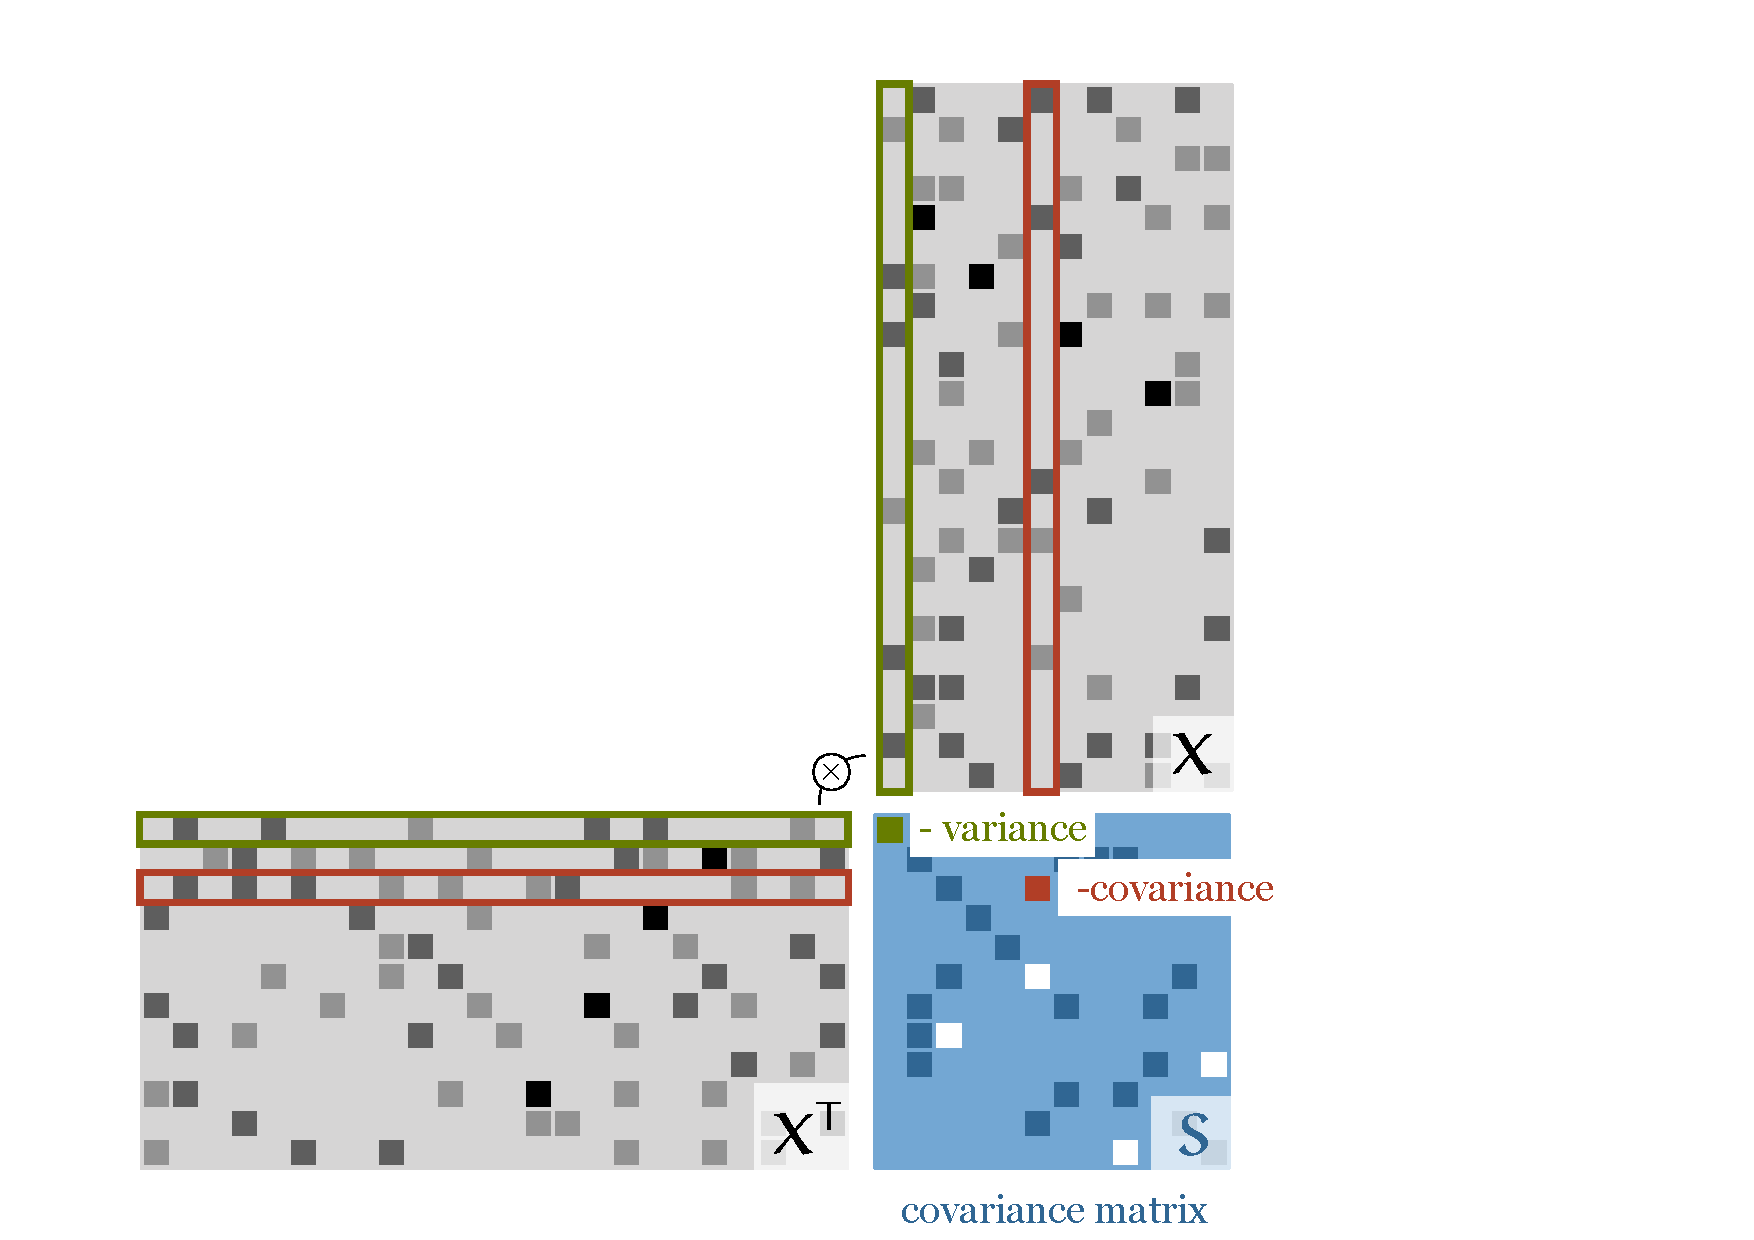
\includegraphics[width=1\textwidth]{./images/pca/covmult.pdf}
	}
\end{figure}

%<figure class="narrow">
%<img src="/images/pca/covmult.svg" class="three-quarters"/>
%</figure>
%
This matrix is symmetric, since \(\text{Cov}(\bc{j}, \bc{k}) = \text{Cov}(\bc{k}, \bc{j})\), and it has the variances of the various features along the diagonal. 

\begin{aside}For any matrix, \(\mbX\) of any size, \(\bc{\mbM} = \mbX^T\mbX\) is square and symmetric: \(\bc{M}_{ij} = \bc{M}_{ij}\) because both values are the dot product of columns \(i\) and \(j\) in the data.
\end{aside}

We'll denote the covariance matrix of our dataset \(\mbX\) by \(\bc{\mbS}\) . This is the matrix that we're interested in: the eigenvectors of \(\bc{\mbS}\) coincide with the principal components of \(\mbX\).

I expect that that doesn't immediately make a lot of intuitive sense. We've developed eigenvectors in terms of matrices that transform points in space. We don't usually think of \(\bc{\mbS}\) as transforming space. It's not common to see a vector multiplied by \(\bc{\mbS}\). Yet, we can easily diagonalize \(\bc{\mbS}\). In fact, since it's symmetric, \gc{the spectral theorem} tells us that we can diagonalize it with an orthogonal matrix, and we can be sure that it has \(\gc{n}\) eigenvalues.

To develop some intuition for what these eigenvalues \emph{mean} we can have a look at the common practice of \textbf{data normalization}.

\section{Data normalization and basis transformations}

Data normalization is a very common data pre-processing step in many data science processes. For many applications we don't much care about the natural scale of the data, and we instead want the data to lie in a predictable range. For one-dimensional data, one way to do this is to rescale the data so that its mean equals \(0\), and its variance equals \(1\). We achieve this easily by first shifting the data so that the mean is at \(0\), and then scaling uniformly until the variance is \(1\).

\index{Normalization}

To work out how to make this transformation, we can imagine that our data \emph{originally} had mean \(0\), and variance \(1\), and was then transformed by scaling and then adding some constant value. That is, every point \(x\) we observed was derived from an unseen point \(z\) by two parameters \(\bc{s}\) and \(\oc{t}\) as 

\[
x = \bc{s}z + \oc{t}
\]

with the \(z\)'s having mean \(0\) and variance \(1\). We will call \(z\) the \textbf{hidden} or \textbf{latent} variable behind the \textbf{observed variable} \(x\).

\index{Latent variable}\index{Hidden variable}\index{Observed variable}

After scaling by \(\bc{s}\), the mean of the "original" data is still \(0\), so we should set \(\oc{t} = \bar x\) to end up with the correct mean for our observed data. To work out \(\bc{s}\), we move this term to the other side:

\[
x - \oc{\bar x} = \bc{s}z \p
\]

The left-hand side is the mean-centered data, and the right hand side is a scaled version of the latent data. Since variance isn't affected by the additive term, we get

\[
\text{Var}(\{x\}) = \kc{\frac{1}{n}}\sum_{z}(\bc{s}z)^2 = \bc{s}^2\kc{\frac{1}{n}}\sum_z z^2 = \bc{s}^2 \times \text{Var}(\{z\}) = \bc{s}^2 
\]

So, to end up with the correct variance for \(x\), we should set the \emph{square} of \(\bc{s}\) equal to the data variance, or equivalently, we should set \(\bc{s}\) equal to the data standard deviation \(\bc{\sigma}\) (the square root of the variance). So, the correct normalization is:

\[
x' = \frac{x - \oc{\bar x}}{\bc{\sigma}} \p
\]

\begin{aside}%
This may seem like an overly elaborate way to derive a pretty intuitive normalization, but we will generalize this approach to higher dimensions later, so it pays to understand the steps. 
\end{aside}

Instead of thinking of this operation as moving the data around, we can also think about it as keeping the data where it is, but just expressing it in different \emph{axes}. We move the origin to coincide with the data mean, and then scale \emph{the unit} (the length of the arrow from \(0\) to \(1\)) so that its tip lies at the point \(\oc{\bar x} + \bc{\sigma}\). On this new axis, the data is normalized.

\begin{figure}[H]
	\centerline{
	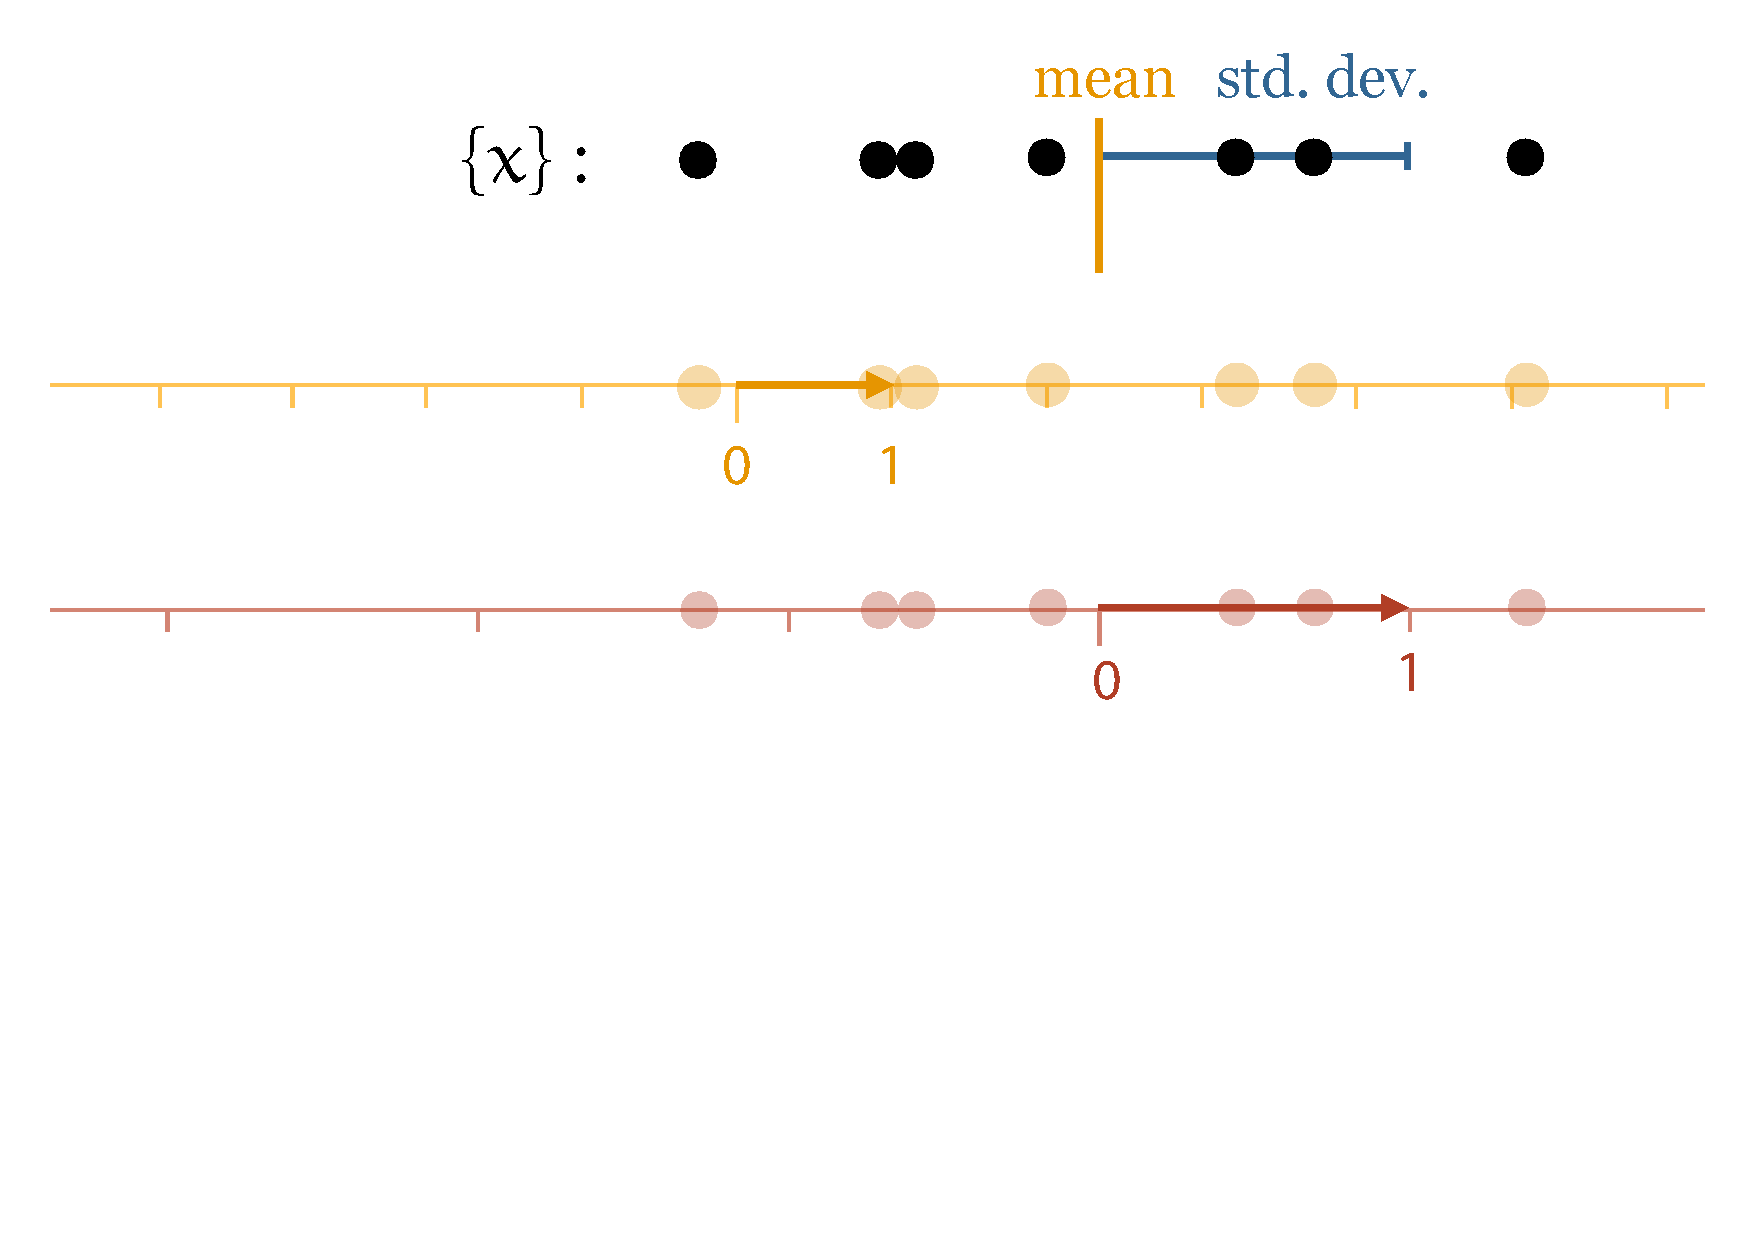
\includegraphics[width=1\textwidth]{./images/pca/onedbasis.pdf}
	}
	\caption*{We can see the operation of normalizing our one-dimensional data as simply expressing the same points on a \rc{different axis}. We change the location of the origin and the length of the unit, and our data is normalized.}
\end{figure}

%<figure class="narrow">
%<img src="/images/pca/onedbasis.svg"/>
%<figcaption>We can see the operation of normalizing our one-dimensional data as simply expressing the same points on a <span class="rc">different axis</span>. We change the location of the origin and the length of the unit (the arrow that points from \(0\) to \(1\)), and our data is normalized.
%</figcaption>
%</figure>
%
In higher dimensions, the \emph{units} we use to express points in space are often called a \emph{basis}. We take a bunch of vectors \(\rc{\mbb}_1, \ldots, \rc{\mbb}_k\), called the \emph{basis vectors} and express points as a sum of the basis vectors, each multiplied by a particular scalar, where the scalars are unique to the point we are expressing.

\begin{aside}Strictly speaking, for the set \(\rc{\mbb}_1, \ldots, \rc{\mbb}_k\) to be a basis, the vectors should also be \emph{linearly independent}. For our current purposes, we don't need to define this so precisely. We'll discuss linear independence in more detail in a later chapter.
\end{aside}

This is how our standard coordinate system works as well: in three dimensions, the basis vectors are \(\oc{\mbe}_1 = (1, 0, 0)\), \(\oc{\mbe}_2 = (0, 1, 0)\) and \(\oc{\mbe}_3 = (0, 0, 1)\). When we refer to a point \(\mbp\) with the coordinates (7, 3, 5), we are implicitly saying that 

\[
\mbp = 
7 \times \oc{\begin{pmatrix}1\\0\\0\end{pmatrix}} + 
3 \times \oc{\begin{pmatrix}0\\1\\0\end{pmatrix}} + 
5 \times \oc{\begin{pmatrix}0\\0\\1\end{pmatrix}}
\]

This is called the \textbf{standard basis}. It's a little elaborate for something so familiar, but it shows a principle we can apply for other sets of basis vectors. With any set of vectors \(\rc{B} = \{\rc{\mbb}_1, \ldots, \rc{\mbb}_k\}\), we can describe a point by writing down a vector \(\mbp^\rc{B}\), and computing

\index{Standard basis}\index{Basis!standard}

\[
\mbp = p_1^\rc{B} \rc{\mbb}_1 + \ldots + p_k^\rc{B} \rc{\mbb}_k 
\]

Here, \(\mbp\) are the coordinates of the point in the \oc{standard basis}, and \(\mbp^\rc{B}\) are the coordinates in the basis \(\rc{B}\).

\vspace{0.5em}
\begin{figure}[H]
	\centerline{
	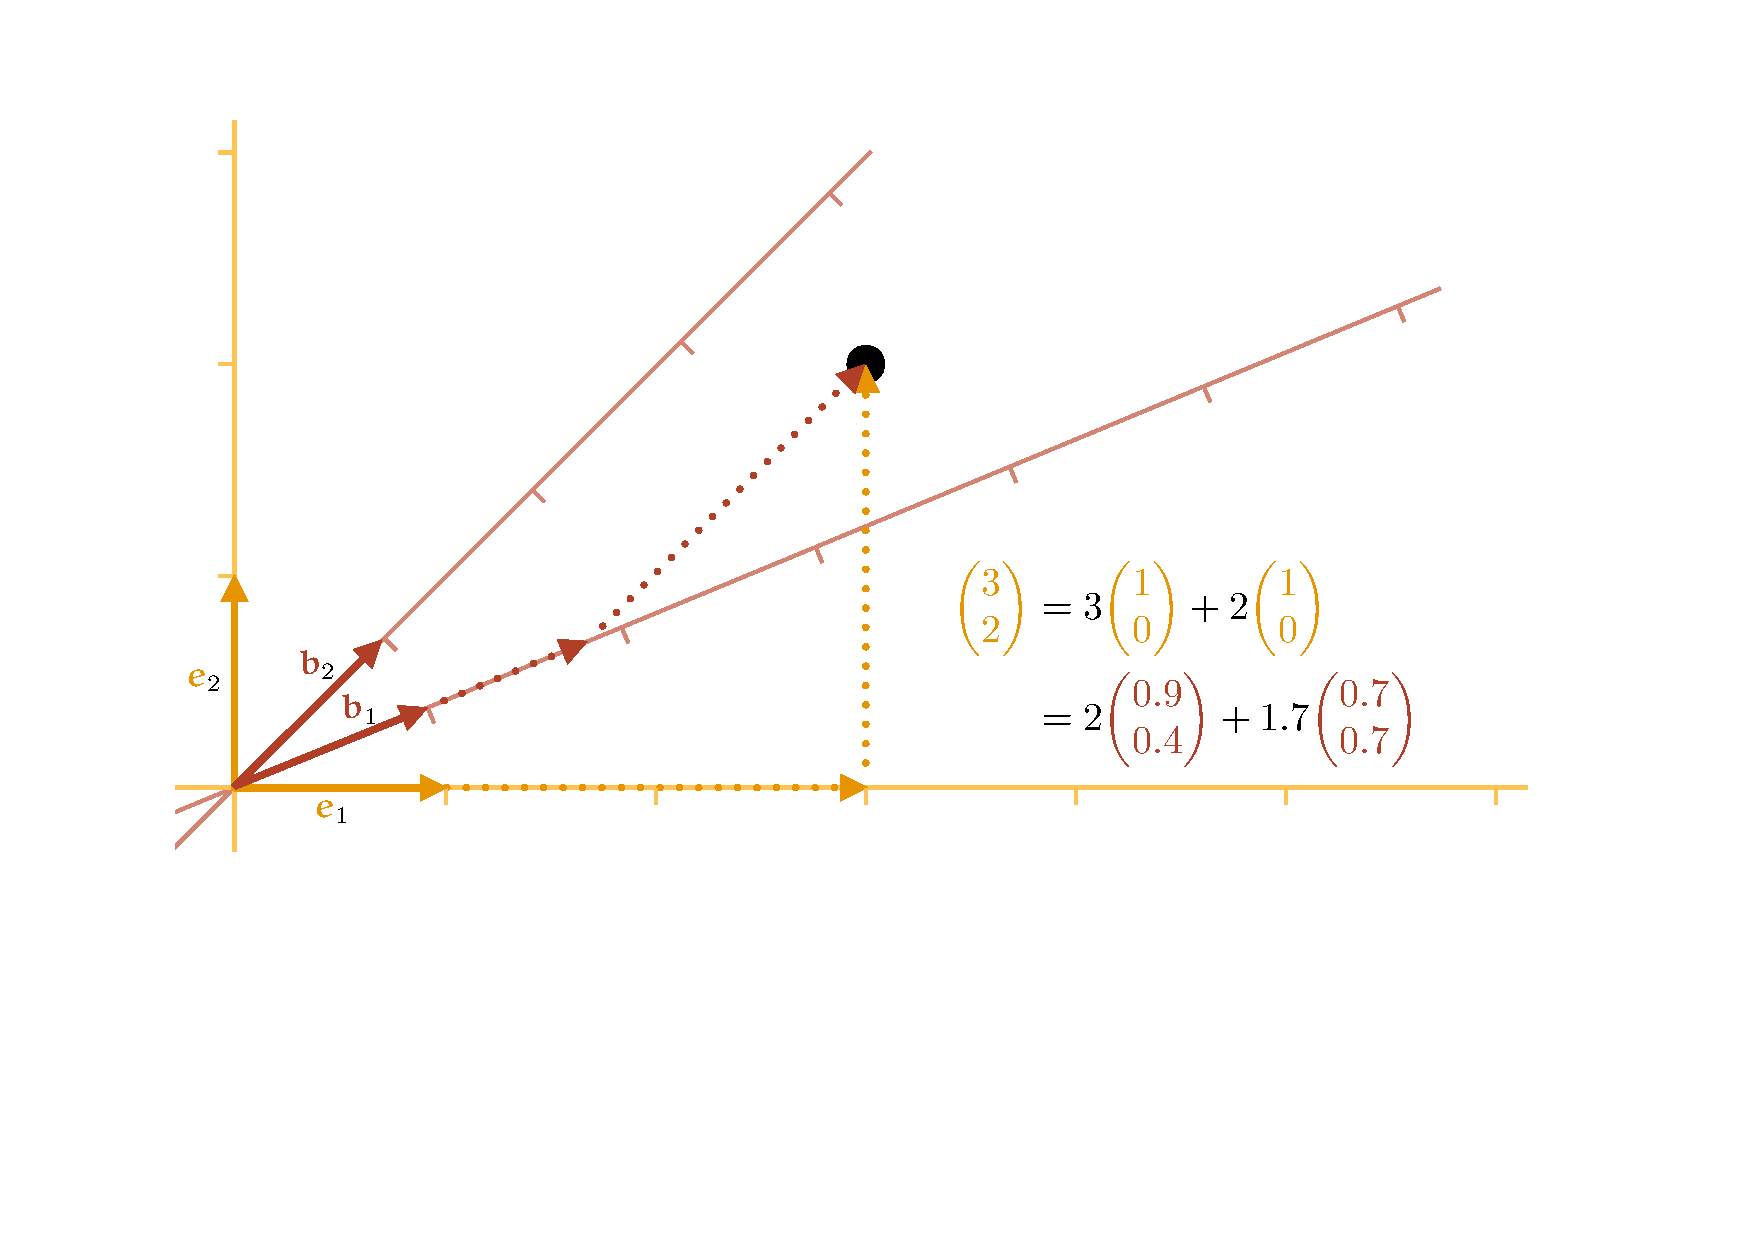
\includegraphics[width=0.7\textwidth]{./images/pca/bases.pdf}
	}
	\caption*{The point \(\oc{(3, 2)}\) as expressed in our \oc{standard basis} becomes the point \(\rc{(2, 1.7)}\) when expressed in the basis defined by vectors \(\rc{\mbb}_1 = (0.9, 0.4)\) and \(\rc{\mbb}_2 = (0.7, 0.7)\).}
\end{figure}

%<figure class="narrow">
%<img src="/images/pca/bases.svg"/>
%<figcaption>The point \(\oc{(3, 2)}\) as expressed in our <span class="oc">standard basis</span> becomes the point \(\rc{(2, 1.7)}\) when expressed in the basis defined by vectors \(\rc{\b}_1 = (0.9, 0.4)\) and \(\rc{\b}_2 = (0.7, 0.7)\).
%</figcaption>
%</figure>

If we concatenate the basis vectors into the columns of a matrix \(\rc{\mbB}\), we can express this transformation as a simple matrix multiplication:
\[
\mbp = \rc{\mbB} \mbp^\rc{B}
\]

This also suggest how to transform in the other direction: from a point in the standard basis to a point in the basis \(\rc{B}\): we require that \(\rc{\mbB}\) is invertible and use
\[
\mbp^\rc{B} = \rc{\mbB}^{-1} \mbp \p
\]

The set of points you can express in a particular basis is called its \textbf{span}. In the image above, the span is the same as that of the standard basis, but if you define two basis vectors in a three-dimensional standard basis, their span would usually be some plane crossing the origin.

\index{Span}

%<!-- 
%<aside>The strict definition of a basis states that a set \(B\) of vectors is only a basis for its span if \(B\) contains no "superfluous" vectors, i.e. vector which we can remove wihout changing the span. Another way of saying this is that no vector in \(B\) can be expressed as a linear combination of one or more of the others.
%</aside>
% -->

If you want to actually compute the transformation into the basis, the computation of a matrix inverse is finicky and very likely to be numerically unstable. It's nice if you can ensure that \(\rc{\mbB}^{-1} = \rc{\mbB}^{T}\). We've seen matrices with this property already: they're called \textbf{orthogonal matrices}. To refresh your memory, orthogonal matrices are square matrices with columns that are all unit vectors and all mutually orthogonal. 

\index{Basis!orthonormal}

\begin{aside}A basis expressed by an orthogonal matrix is called an orthonormal basis. It's a rotated or flipped version of the standard basis, but the basis vectors are still all orthogonal and they are still all unit vectors.
\end{aside}

We can now say that our data normalization was nothing more than a simple basis transformation in \({\mathbb R}^1\). We mean-center the data, and replace the standard basis vector by one that matches the variance of our data. This is not an orthonormal basis, but we'll see a fix for that later.

More importantly, we can translate the idea of data normalization to higher dimensions. 

In  \({\mathbb R}^1\), we were after a basis in which the variance was 1. In \({\mathbb R}^n\) we will look for a basis in which the \emph{covariance} is \(\mbI\). 

\pagebreak  
\noindent This requirement has two consequences: 
\begin{itemize}
\item In our new coordinates, the variance is \(1\) along all axes.
\item In our new coordinates all covariances are \(0\). That is, the data is perfectly \emph{decorrelated}.
\end{itemize}

\index{Decorrelated}

\begin{aside}This kind of normalization is called \emph{whitening} (because standard normally distributed noise is sometimes called white noise). It's not usually necessary in data science, but it can be a very powerful preprocessing method if you can spare the required resources. We're primarily discussing it as a way of making intuitive what is happening under the hood of PCA.
\end{aside}

\index{Whitening}

We'll proceed the same way we did before: we will imagine that our data was originally of this form, and has been transformed by an affine transformation. We'll call  the matrix for this imagined  ``original'' data \(\mbZ\). This means that we assume that \(\mbX\) was produced by sampling \(\mbZ\) from a standard normal distribution and transforming with as:

\[
\mbX^T = \bc{\mbA}\mbZ^T + \oc{\mbt}
\]
with some $\bc{\mbA}$ and $\oc{\mbt}$.

As before, we will first figure out which \(\bc{\mbA}\) and which \(\oc{\mbt}\) will take us from the latent data \(\mbZ\) to our observed data \(\mbX\), and then we will invert this transformation to find the transformation that normalizes our data.

The logic for \(\oc{\mbt}\) is the same as it was before: since \(\mbZ\) has zero mean, it still has zero mean after being transformed by \(\bc{\mbA}\). If we set \(\oc{\mbt} = \bar\mbx\), we transport this to the mean of the observed data.

We move this term to the left-hand side

\[
\mbX^T - \oc{\bar\mbx} = \bc{\mbA}\mbZ^T
\]

and observe that the mean-centered data on the left is equal to our \(\bc{\mbA}\)-transformed latent data.

Now, we need to set \(\bc{\mbA}\) to achieve the right covariance. The covariance is unaffected by the additive term \(- \oc{\bar \mbx}\), so we can ignore that. The covariance of the transformed data is:

\[
\text{Cov}(\mbX) = \kc{\frac{1}{n}} \bc{\mbA}\mbZ^T(\bc{\mbA}\mbZ^T)^T = \kc{\frac{1}{n}} \bc{\mbA}\mbZ^T\mbZ\bc{\mbA}^T = \bc{\mbA}\kc{\text{Cov}(\mbZ)}\bc{\mbA}^T = \bc{\mbA}\bc{\mbA}^T \p
\]

Where previously we needed to choose our scalar \(\bc{s}\) so that its square was equal to the data variance \(\bc{\sigma}^2\), we now need to choose our transformation matrix \(\bc{\mbA}\) so that its ``square'' \(\bc{\mbA}\bc{\mbA}^T\) is equal to the data \emph{co}variance \(\bc{\mbS}\).

If we find such an \(\bc{\mbA}\), we know that its \emph{transformation} is what maps the decorrelated data to the data we've observed. So even though we never transform any points by the covariance matrix, we see that internally, it does contain a very natural transformation matrix.

There are a few ways to find \(\bc{\mbA}\) for a given \(\bc{\mbS}\). The Cholesky decomposition is the most natural analogue to the square root we used in the 1D case. This road leads to a technique known as \emph{Cholesky whitening}.

\index{Whitening!Cholesky}\index{Cholesky whitening}

But this is not a book about whitening, it's a book about PCA. We're trying build some intuition for what PCA is doing. So instead, we'll solve \(\bc{\mbS} = \bc{\mbA}\bc{\mbA}^T\) using the orthogonal diagonalization we developed earlier, which will lead us to a method called \emph{PCA whitening} (a kind of byproduct of the PCA analysis).

\index{Whitening!PCA}\index{PCA!Whitening}

We know that \(\bc{\mbS}\) is square and symmetric, so we know it can be orthogonally diagonalized:

\[
\bc{\mbS} = \rc{\mbP}\bc{\mbD}\rc{\mbP}^T \p
\]

To turn this into a solution to \(\bc{\mbS} = \bc{\mbA}\bc{\mbA}^T\) we need two factors, with the second the transpose of the first. We can do this easily by noting two things about the diagonal matrix in the middle. First, the square root $\bc{\mbD}^\frac{1}{2}$ of a diagonal matrix $\bc{\mbD}$ is just another diagonal matrix with the square roots of the original elements along the diagonal. This gives us \(\bc{\mbD} = \bc{\mbD^\frac{1}{2}}\bc{\mbD^\frac{1}{2}}\). Second, the transpose of a diagonal matrix is the same matrix, so that \(\bc{\mbD} = \bc{\mbD^\frac{1}{2}}{\bc{\mbD^\frac{1}{2}}}^T\). Thus

\index{Matrix square root}\index{Square root!of a matrix}\index{$\bc{\mbA}^\frac{1}{2}$}

\begin{align*}
\bc{\mbS} &= \rc{\mbP}\bc{\mbD^\frac{1}{2}}{\bc{\mbD^\frac{1}{2}}}^T\rc{\mbP}^T \\
&= \bc{\mbA}\bc{\mbA}^T \hspace{2em}\text{with } \bc{\mbA} = \rc{\mbP}\bc{\mbD^\frac{1}{2}}
\end{align*}

Finally, to whiten our data, we reverse the transformation from \(\mbZ\) to \(\mbX\) and get 

\[
\mbZ = \bc{\mbA}^{-1}(\mbX - \oc{\mbt}) = \bc{\mbD}^{-\frac{1}{2}}\rc{\mbP}^T (\mbX - \oc{\mbt}) \p
\]

So, to map our data to a zero-mean, unit-variance, decorrelated form, we map to the basis formed by the eigenvectors of \(\bc{\mbS}\) and then divide along each axis  by the square root of the eigenvalues. We can see here that the eigenvalues of the covariance matrix are the variances of the data, \emph{along the eigenvectors} (remember that we divided by the square of the variance before).

Taking the alternative perspective we took above, we can also keep the data where it is and \emph{change our basis}. We scale the standard basis along the axes by   \(\bc{\mbD}^{\frac{1}{2}}\) rotate by \(\rc{\mbP}\) and translate by \(\oc{\bar \mbx}\). In the resulting axes, our data has mean \(\mathbf 0\), and covariance \(\mbI\).


\begin{figure}[H]
	\centerline{
	\includesvg[width=1\textwidth]{./images/pca/covariance-2.svg}
	}
\end{figure}

%<figure class="narrow">
%<img src="/images/pca/covariance-2.svg" />
%</figure>

\begin{aside}%
Note how we're having our cake and eating it too. We are scaling our axes to control the variance, so we can't have an orthonormal basis, but the eigendecomposition breaks the basis transformation in two steps: first an orthonormal basis transformation, which allows us to use $\rc{\mbP}^T$ instead of $\rc{\mbP}^{-1}$, and then a scaling along the new axes by the eigenvalues.
\end{aside}


\section{Quadratic forms}

Have we fully married our first intuition about eigenvectors in transformation matrices with the role eigenvectors play in PCA, as the eigenvectors of \(\bc{\mbS}\)? Not quite. We've shown that \(\bc{\mbS}\) is in some sense composed of a very important transformation \(\bc{\mbA}\), which transforms decorrelated data with unit variance to have covariance \(\bc{\mbS}\), but the eigenvectors we're using are not the eigenvectors of \(\bc{\mbA}\). Rather,  \(\bc{\mbA}\) is \emph{made up} of our eigenvectors and may itself have different eigenvectors, or no (real) eigenvectors at all.

\begin{aside}%
We will see in Chapter~\ref{chapter:svd} that the eigenvectors of $\bc{\mbS}$ are called the \emph{singular} vectors of $\bc{\mbA}$.
\end{aside}

\index{Singular vectors}

To develop an intuition for how \(\bc{\mbS}\) operates on space, it's more helpful not to look at the linear form

\[\bc{\mbS}\mbx\]

but at the \emph{quadratic} form 

\[\mbx^T\bc{\mbS}\mbx \p\]

\index{Quadratic form}

This may look mysterious, but it's just a concise way of writing second-order polynomials in \(n\) variables (just like \(\mbM\mbx\) is a concise way of writing a linear function from \(n\) to \(m\) variables). For instance,

\[
\mbx^T\begin{pmatrix}\rc{2}& \bc{3}\\ \gc{4}& \oc{5} \end{pmatrix}\mbx = \rc{2}{x_1}^2 + \bc{3}x_2 x_1  + \gc{4} x_1x_2 + \oc{5}{x_2}^2
\]

The simplest quadratic is \(\mbx^T\mbI\mbx\), or just \(\mbx^T\mbx\). If we set this equal to 1, the points that satisfy the resulting equation are the unit vectors. In 2 dimensions, these form a circle called the bi-unit circle. In higher dimensions, the resulting set is called the bi-unit (hyper)sphere. 

\index{Bi-unit!circle}\index{Bi-unit!sphere}

\noindent There are two ways to use quadratic forms to study the eigenvectors of \(\bc{\mbS}\). The first is to look at \(\mbx^T\bc{\mbS}\mbx\) and to study what this function looks like when constrained to the bi-unit sphere. Looking only at the points for which \(\mbx^T\mbx = 1\) what happens to the parabola \(\mbx^T\bc{\mbS}\mbx\)?

\vspace{-3.5em}
\begin{figure}[H]
	\centerline{
	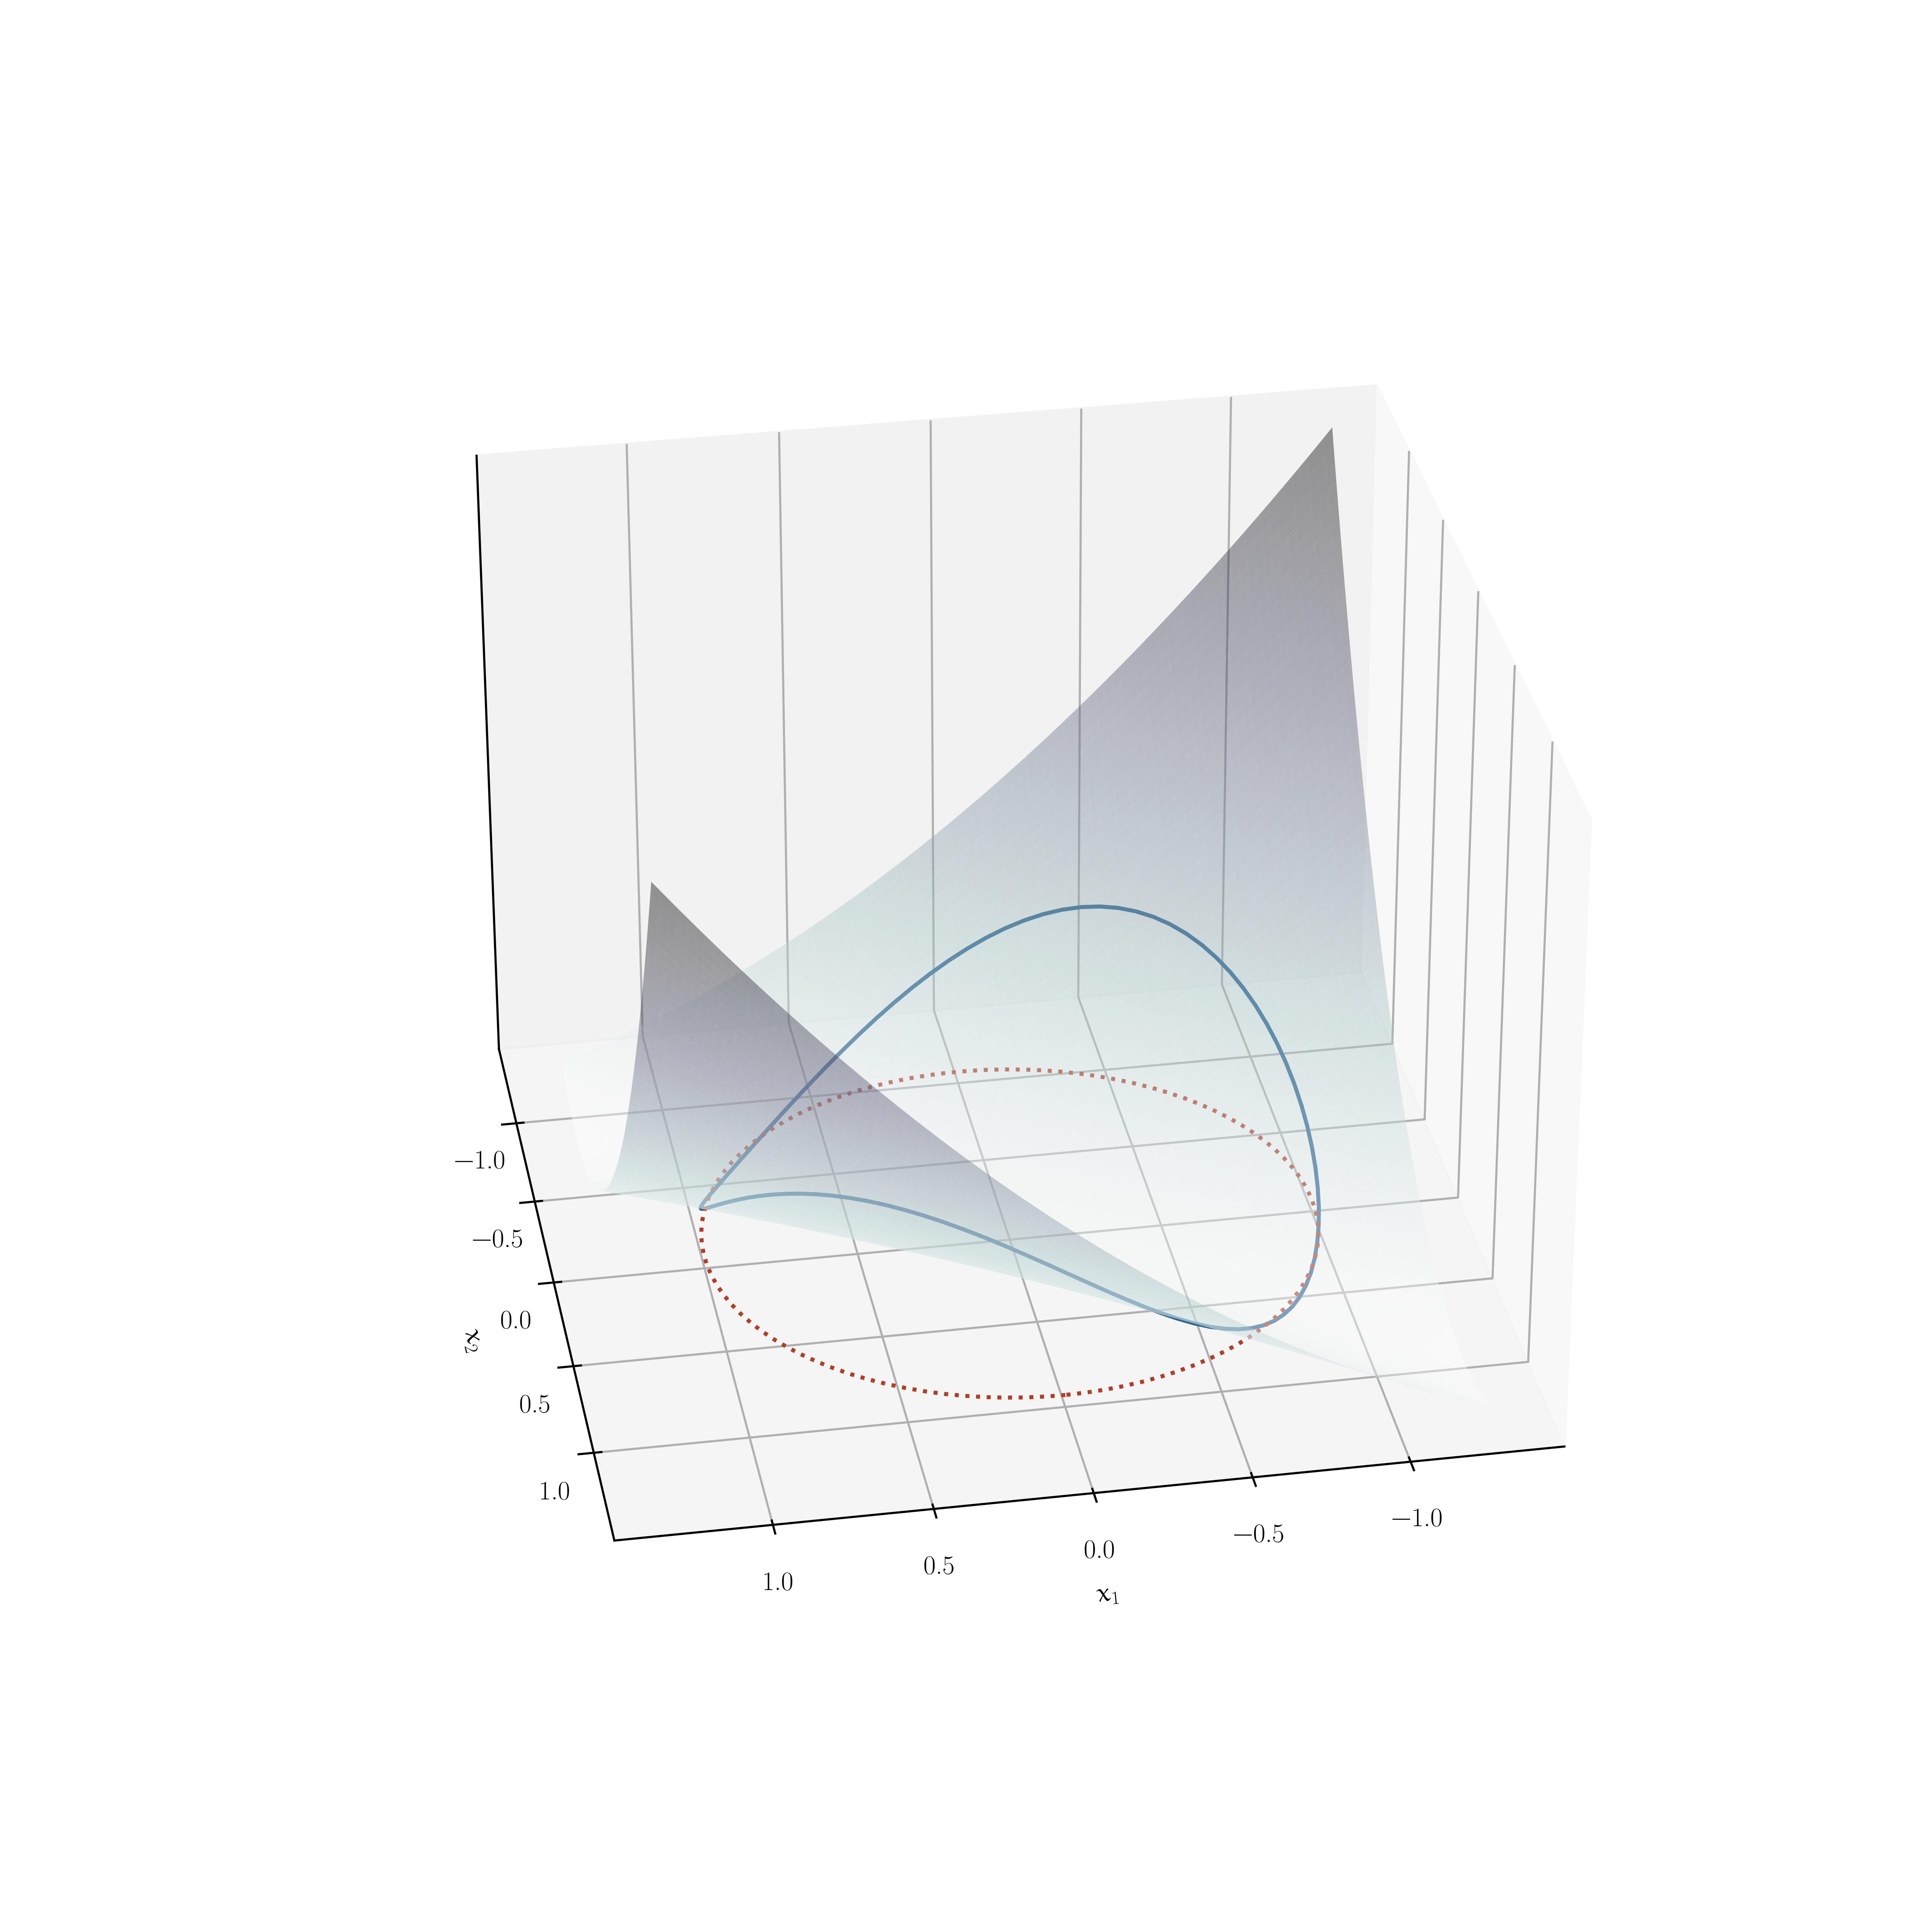
\includegraphics[width=1.2\textwidth]{./images/pca/surface.png}
	\vspace{-3.5em}
	}
	\caption*{The \bc{bi-unit circle} is deformed by the parabola \(\mbx^T\begin{pmatrix}\rc{2}& \bc{3}\\ \gc{4}& \oc{5} \end{pmatrix}\mbx\)}
\end{figure}
%<figure class="narrow">
%<img src="/images/pca/surface.svg"/>
%<figcaption>The <span class="rc">bi-unit circle</span> is deformed by the parabola \(\x^T\begin{pmatrix}\rc{2}& \bc{3}\\ \gc{4}& \oc{5} \end{pmatrix}\x\). 
%</figcaption>
%</figure>

If we diagonalize \(\bc{\mbS} = \rc{\mbP}\bc{\mbD}\rc{\mbP}^T\), the quadratic becomes \(\mbx^T\rc{\mbP}\bc{\mbD}\rc{\mbP}^T\mbx\). The first and last two factors are just a change of basis so we can also write \(\mbz^T\bc{\mbD}\mbz\) with \(\mbz = \rc{\mbP}^T\mbx\). Since \(\rc{\mbP}\) is orthogonal, the change of basis doesn't change the length of the vectors and the constraint that \(\mbx\) should be unit vectors is equivalent to requiring that \(\mbz\) be unit vectors.

\noindent The quadratic form \(\mbz\bc{\mbD}\mbz\) is particularly simple, because \(\bc{\mbD}\) is diagonal. We simply get 

\[
\mbz\bc{\mbD}\mbz = z_1z_1\bc{D}_{11} + z_2z_2\bc{D}_{22} + \ldots + z_\bc{m}z_\bc{m}\bc{D}_\bc{mm} \p
\]

\index{Quadratic form!of a diagonal matrix}

This sum is very important. Note that all the factors \(z_\bc{r}z_\bc{r}\) are not only positive (because they're squares), but they also sum to one, since \(\|
\mbz\|^2  = {z_1}^2 + \ldots + {z_\bc{m}}^2\) is the squared length of vector \(\mbz\), which we constrained to \(1\).

We'll call this a \textbf{weighted sum}: a sum over some set of numbers where each term is multiplied by a positive weight, so that the weights sum to \(1\).

\index{Weighted sum}

%<!--
% We can explain why S is acting on space as a quadratic transform and why maximizing the quadritic form maximizes the variance. Double check and add this.
% -->

In the next section, we will use this sum to prove just about every open question we have left. For now, just notice what happens when \(\mbx\) is an eigenvector. In that case, \(\mbz\) is a one-hot vector, because \(\rc{\mbP}\mbz = \mbx\), and only one of the terms in the sum is non-zero.

\index{One-hot vector}

This is one way to think of the quadratic form of \(\bc{\mbS}\): it defines \(\bc{m}\) \rc{orthogonal directions in space} (the eigenvectors), at which the quadratic takes some \bc{arbitary value} (the eigenvalues). For all other directions \(\mbx\), the quadratic is a weighted mixture  between the eigenvalues, with the weights determined by how much of \(\mbx\) projects onto the corresponding eigenvectors.

\begin{aside}Looking at the sum above, you may be able to figure out what the minimum and maximum values are of the quadratic form \(\mbx^T\bc{\mbS}\mbx\) under the constraint that \(\mbx^T\mbx = 1\). Note the similarity of this optimization problem to the PCA problem. If you don't see it yet, don't worry. We'll dig deeper into this in the next section.
\end{aside}

For another geometric interpretation of the  eigenvectors of \(\bc{\mbS}\), think back to the one-dimensional example of normalizing data. 

In the normalized version of the data, the variance is equal to \(1\). This means that, for most distributions, we can be sure that the majority of the data lies in the interval \((-1, 1)\). This is called the bi-unit interval, since it is made up of two units around the origin. If our data is normally distributed, this interval captures about 68\% of it after normalization. The transformation by \(\oc{t}\) and \(\bc{s}\) maps this interval to an interval that captures the same proportion of the unnormalized data.

\index{Bi-unit!interval}

\noindent In higher dimensions, the analogue of the bi-unit interval is the bi-unit sphere, the set of all points that are at most \(1\) away from the origin. To follow the analogy, we can transform the bi-unit sphere, which captures the majority of \(\mbZ\), by some \(\bc{\mbA}^{-1}\) so that we capture the majority of the observed data $\mbX$.

\index{Bi-unit!sphere}

\begin{figure}[H]
	\centerline{
	\includesvg[width=1\textwidth]{./images/pca/covariance-ellipses.svg}
	}
	\caption*{The \oc{bi-unit circle} captures the majority of the normalized data. The \rc{ellipse} we create by transforming the circle by \(\bc{\mbA}^{-1}\) (and translating to the mean) captures the same majority of the \gc{unnormalized data}.}
\end{figure}

%<figure class="narrow">
%<img src="/images/pca/covariance-ellipses.svg" />
%<figcaption>The <span class="oc">bi-unit circle</span> captures the majority of the normalized data. The <span class="rc">ellipse</span> we create by transforming the circle by \(\bc{\A}^{-1}\) (and translating to the mean) captures the same majority of the <span class="gc">unnormalized data</span>.
%</figcaption>
%</figure>

In two dimensions, the transformation by \(\bc{\mbA}\) and \(\oc{\mbt}\) that we derived above is the transformation that maps the bi-unit circle to an ellipse which captures the majority of the data. In more than two dimensions, we're mapping a hypersphere to an \emph{ellipsoid}.

\index{Ellipsoid}

\noindent Note that the standard basis vectors are mapped to the eigenvectors of \(\bc{\mbS}\). We call this new basis, in which the data is normalized, the \textbf{eigenbasis} of \(\bc{\mbS}\).

\index{Eigenbasis}

To work out the shape of the ellipsoid in quadratic form, we just start with the set of all unit vectors \(C = \left \{ \mbu :\mbu^T\mbu = 1 \right\}\) and transform each by \(\bc{\mbA}\) individually (much like we transformed the Mona Lisa earlier).

\vspace{-1em}
\begin{align*}
\bc{\mbA}C &= \left \{\bc{\mbA}\mbu : \mbu^T\mbI\mbu = 1 \right\} & \\
& = \left \{\mby : \mbu^T\mbu = 1 \;\;\text{and}\;\; \mby = \bc{\mbA}\mbu \right\} & \\
& = \left \{\mby :  \left ( \bc{\mbA}^{-1} \mby \right ) ^T \bc{\mbA}^{-1}\mby = 1\right \} & \\
& = \left \{\mby :  \mby^T \bc{\mbS}^{-1} \mby  = 1 \right\} &
\end{align*}

That is, to transform the bi-unit circle to an ellipsoid that covers the same proportion of \(\mbX\) as the circle did of \(\mbZ\), we turn the equation \(\mbu^T\mbu = 1\) into the equation \(\mby\bc{\mbS}^{-1}\mby = 1\). This gives us a quadratic form that desribes the ellipsoid that covers the majority of our data.

Why do we get an inversion from \(\bc{\mbS}\) to \(\bc{\mbS}^{-1}\)? Follow the transformation along the first eigenvector of \(\bc{\mbS}\). In this direction, we are multiplying the input unit vector by the square of the first eigenvalue (remember \(\bc{\mbA} = \rc{\mbP}\bc{\mbD}^\frac{1}{2}\)). To keep the vector a unit vector, we should therefore \emph{divide} by the square of the first eigenvalue. In other words, if we want to define a quadratic form for which the arguments transformed by \(\bc{\mbA}\) stay unit vectors, then the more the value of \(\mbx^T\bc{\mbS}\mbx\) grows, the more our quadratic form should shrink and vice versa.

\begin{aside}Note that the inverse of a symmetric matrix has a particularly simple expression in terms of its orthogonal diagonalization: \(\bc{\mbS}^{-1} = \left(\rc{\mbP}\bc{\mbD}\rc{\mbP}^T\right)^{-1} = \rc{\mbP}\bc{\mbD}^{-1}\rc{\mbP}^T\). That is, the eigenvectors stay the same, and we just take the reciprocals of the eigenvalues.
\end{aside}

\section{Why is PCA optimal?}

With the quadratic form added to our toolbox, we can finally start answering some of the deeper questions. Both visually, using transformations of ellipses, and formally, using the language of eigenvectors.

Let's start simply: why does the first principal component coincide with an eigenvector of \(\bc{\mbS}\)? And, while we're at it, which eigenvector does it coincide with?

Visually, this is easy to show. In the image above, we plotted the bi-unit circle, and its transformation into an ellipse that covers the same part of the observed data. The \oc{standard basis vectors} are mapped to the eigenvectors. Note that these become the axes of \rc{the ellipse}. One of the standard basis vectors is mapped to the ellipse's \emph{major axis}, the direction in which it bulges the most.The direction in which the data bulges the most is also the direction of greatest variance, and therefore the first principal component.

The proof of this fact is not very complex.

\begin{theorem}[First eigenvector.] The first principal component is the eigenvector of the covariance matrix \(\bc{\mbS}\) with the largest eigenvalue.
\end{theorem}
\begin{proof} The first principal component \(\rc{\mbw}_1\) is defined as 

\[
\argmax{\rc{\mbw}} \sum_\gc{i} \left(\rc{\mbw}^T\mbx_\gc{i}\right)^2 \\
\;\;\text{such that } \rc{\mbw}^T\rc{\mbw} = 1
\]

that is, the direction in which the variance of the projected data is maximized.

Rewriting the objective function, we get

\begin{align*}
 \sum_\gc{i} \left(\rc{\mbw}^T\mbx_\gc{i}\right)^2 &= \sum_\gc{i} \rc{\mbw}^T\mbx_\gc{i}\mbx_\gc{i}^T\rc{\mbw} \\
 &= \rc{\mbw}^T\left(\sum_\gc{i} \mbx_\gc{i}\mbx_\gc{i}^T\right)\rc{\mbw} \\
 &= \rc{\mbw}^T \mbX^T\mbX \rc{\mbw} \\
 &= \kc{N} \rc{\mbw}^T \bc{\mbS} \rc{\mbw} \p
\end{align*}

This means that the direction in which the sum of variances is maximized, is the direction, represented by a unit vector \(\rc{\mbw}\), for which the quadratic form \(\rc{\mbw}^T\bc{\mbS}\rc{\mbw}\) is maximal.

\noindent If we orthogonally diagonalize \(\bc{\mbS}\), with the eigenvalues canonically arranged, we get

\begin{align*}
\rc{\mbw}^T \bc{\mbS} \rc{\mbw} &= \rc{\mbw} ^T\rc{\mbP}\bc{\mbD}\rc{\mbP}^T \rc{\mbw} \\
&= \mbz\bc{\mbD}\mbz \;\;\text{with } \mbz = \rc{\mbP}^T\rc{\mbw} \p
\end{align*}

In the last step, we've simplified to a diagonal quadratic form in the eigenbasis of \(\bc{\mbS}\). This quadratic form simplifies to

\[
\mbz^T\bc{\mbD}\mbz = {z_1}^2 \bc{D}_{11} + \ldots + {z_\bc{m}}^2\bc{D}_\bc{mm}
\]

where the constraint that \(\mbz\) is a unit vector means that \({z_1}^2 + \ldots + {z_\bc{m}}^2 = 1\). In other words, this is a weighted sum over the diagonal elements of \(\bc{\mbD}\). To maximize a weighted sum, we assign weight \(1\) to the largest element and weight \(0\) to the rest. Since we took \(\bc{D}_{11}\) to be the largest eigenvalue, the vector \(\hat\mbz = (1, 0, \ldots, 0)\) maximizes the quadratic form.

\index{Weighted sum}

Mapping back to the standard basis, we get \(\rc{\mbw}_1 = \rc{\mbP}\hat\mbz\). That is, the first column of \(\rc{\mbP}\), which is the first eigenvector of \(\bc{\mbS}\). \hfill\qed
\end{proof}

We can extend this proof to show that all the other PCs are eigenvectors as well.

\begin{theorem}[PCs as eigenvectors.] The \(\rc{k}\)-th principal component of \(\mbX\) is the \(\rc{k}\)-th eigenvector of the covariance matrix \(\bc{\mbS}\).
\end{theorem}
\begin{proof} For the first principal component \(\rc{\mbw}_1\), the previous theorem provides a proof. For \(\rc{\mbw}_2\), follow the previous proof until the  weighted sum

\[
\mbz^T\bc{\mbD}\mbz = {z_1}^2 \bc{D}_{11} + \ldots + {z_\bc{m}}^2\bc{D}_\bc{mm} \p
\]

First, note that any vector \(\rc{\mbw}'\) that is orthogonal to \(\rc{\mbw}_1\) must also be orthogonal after transformation by \(\rc{\mbP}\rc{\mbP}^T\):
\enlargethispage{1.5em}

\[
0 = \rc{\mbw}_1^T\rc{\mbw}' = {\rc{\mbw}_1}^T\rc{\mbP}\rc{\mbP}^T\rc{\mbw}' = {\mbz_1}^T\mbz' \p
\]

Thus, the second eigenvector is orthogonal to the first (as required) if and only if their projections by \(\rc{\mbP}^T\) are orthogonal as well (and similarly for higher eigenvectors). 


Recall that the \(\mbz\)-vector of the first principal component is \((1, 0, \ldots, 0)\), so to be orthogonal, the \(\mbz\) vector corresponding to the second principal component must have \(0\) at its first element. Since the \(\bc{D}_{jj}\) are arranged in decreasing order, we maximize the sum under this constraint with the vector \(\hat \mbz = (0, 1, 0, \ldots, 0)\). \(\rc{\mbP}^T \hat\mbz\) selects the second column in \(\rc{\mbP}\), so the second principal component coincides with the second eigenvector.

The same logic holds for the other principal components. For each component \(\rc{r}\), we must set all weights \({z_i}^2\) with \(i < \rc{r}\) to zero in order for the \(\mbz\) vector to be orthogonal to all principal components already chosen. In the remainder of the sum, we maximize the weight with the one-hot vector for \(\rc{r}\), which selects the \(\rc{r}\)-th eigenvector.\hfill\qed
\end{proof}

We have finally shown that the eigenvectors are the vectors that maximize the variance. 

There is one question left to answer: Why is the set of the first \(\rc{k}\) principal components a solution to the combined problem at \(\rc{k}\)?

\begin{theorem}[Optimality of PCA.] For any \(\rc{k}\), a solution to the iterative problem is a solution to the combined problem.
\end{theorem}
\begin{proof} Let \(\rc{\mbW}\) be a solution to the combined problem at \(\rc{k}\). Let \(\mbz_1, \ldots, \mbz_\rc{k}\) be the columns of \(\rc{\mbP}^T\rc{\mbW}\), that is, the solution vectors expressed in the eigenbasis of \(\bc{\mbS}\). The total variance captured by all these \(\mbz\) is

\[\sum_\rc{r} \mbz_\rc{r}^T\bc{\mbS}\mbz_\rc{r} = \sum_{\rc{r}, \bc{j}}  {z_{\rc{r}\bc{j}} }^2\bc{D}_\bc{jj} \p
\]

Where \(z_{\rc{r}\bc{j}}\) is the \(\bc{j}\)-th element of vector \(\mbz_\rc{r}\). These are \(\rc{r}\) weighted sums, summed together. We can group the weights that each \(\mbz_\rc{r}\) contributes to each eigenvalue \(\bc{D_{jj}}\) in to a single sum:

\[
\sum_{\rc{r}, \bc{j}} {\mbz_\rc{r}}^2\bc{D}_\bc{jj} =  \sum_\bc{j} \bc{D_{jj}} \sum_\rc{r}{z_{\rc{r}\bc{j}} }^2 \p
\]

Now, since the different \(\mbz_\rc{r}\)'s are orthogonal, and each of unit length, their sum contribution to each \(\bc{D_{jj}}\) must be no more than \(1\), and the sum of each of their weights is 1.

Why? Imagine the matrix \(\mbZ\) with the \(\mbz_\rc{r}\)for its columns. What we're saying is that its squared elements of \(\mbZ\) should sum to 1 over the columns and not exceed 1 when summed over the rows. If we take \(\mbZ^T\mbZ\), the squared and summed columns end up along the diagonal. We know \(\mbZ^T\mbZ = \mbI\), so these are all \(1\).

If we take \(\mbZ\mbZ^T\), the squared and summed \emph{rows} end up along the diagonal. Extend \(\mbZ\) with orthogonal unit vectors until it is square and orthogonal. Then \(\mbZ\mbZ^T = \mbI\). Each \(1\) on the diagonal of \(\mbI\) is the result of a sum of squared values. Some come from the original \(\mbZ\), some from the columns we added, but all are squares, so it's a sum of nonnegative terms. Therefore, the terms contributed by the original vectors cannot sum to more than \(1\).


\begin{figure}[H]
	\centerline{
	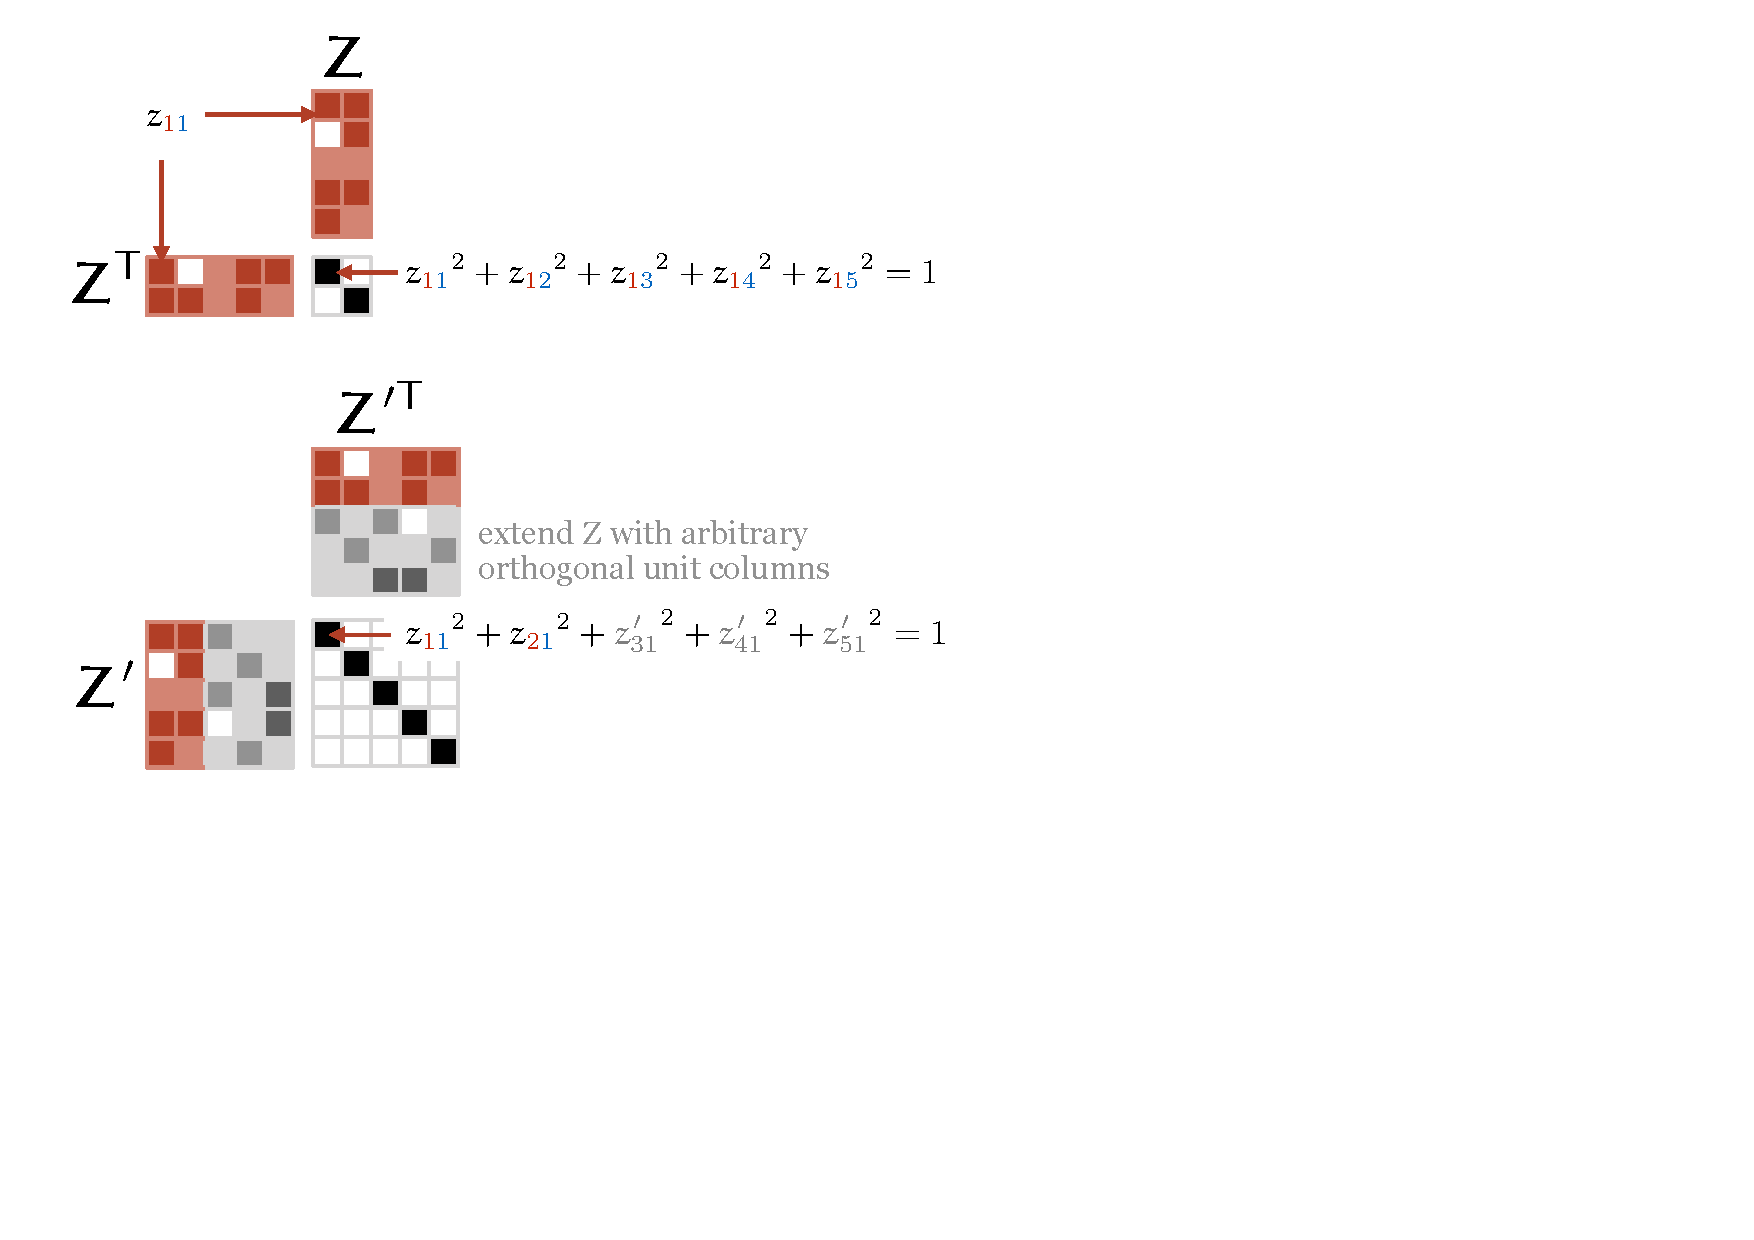
\includegraphics[width=1\textwidth]{./images/pca/zbounds.pdf}
	}
\end{figure}

%<figure class="narrow">
%<img src="/images/pca/zbounds.svg" class="three-quarters" />
%</figure>
%
So, we have a weighted sum where the total weight allowed is \(\rc{k}\), and the maximum weight per element is \(1\). The optimal solution is to give a maximum weight of \(1\) to each of the largest \(\rc{k}\) elements---that is, the first \(\rc{k}\) eigenvalues---and zero weight to everything else. 

\index{Weighted sum}

One way to achieve this is by setting \(\{\mbz_\rc{r}\}\) to be the first \(\rc{k}\) one-hot vectors, which yield the first \(\rc{k}\) eigenvectors when we transform back to the standard basis.\hfill\qed
\end{proof}

Note that when we say ``one way'' in the last paragraph, we do not mean the \emph{only} way. For instance, if we set \(\rc{k} = 2\), we get an optimum with \(\mbz_1 = (1, 0, 0, \ldots), \mbz_2 = (0, 1, 0, \ldots)\) (the PCA solution), but rotating the vectors by 45 degrees in their shared plane gives us \(\mbz_1 = (\sqrt{\small 1/2}, \sqrt{\small 1/2}, 0, \ldots), \mbz_2 = (\sqrt{\small 1/2}, -\sqrt{\small 1/2}, 0, \ldots)\). Filling these values into the sum, we see that they also result in a weight of \(1\) for \(\bc{D_{11}}\) and a weight of \(1\) for \(\bc{D_{22}}\), which means that this is also a solution to the combined problem at \(\rc{k}=2\).

More broadly, given the PCA solution, any other \(\rc{\mbW}\) whose columns span the same space as the span of the PCA solution is also a solution to the combined problem.

We have finally proved our Venn diagram correct, and we have illustrated what the rest of the light blue circle is made of.

\begin{figure}[H]
	\centerline{
	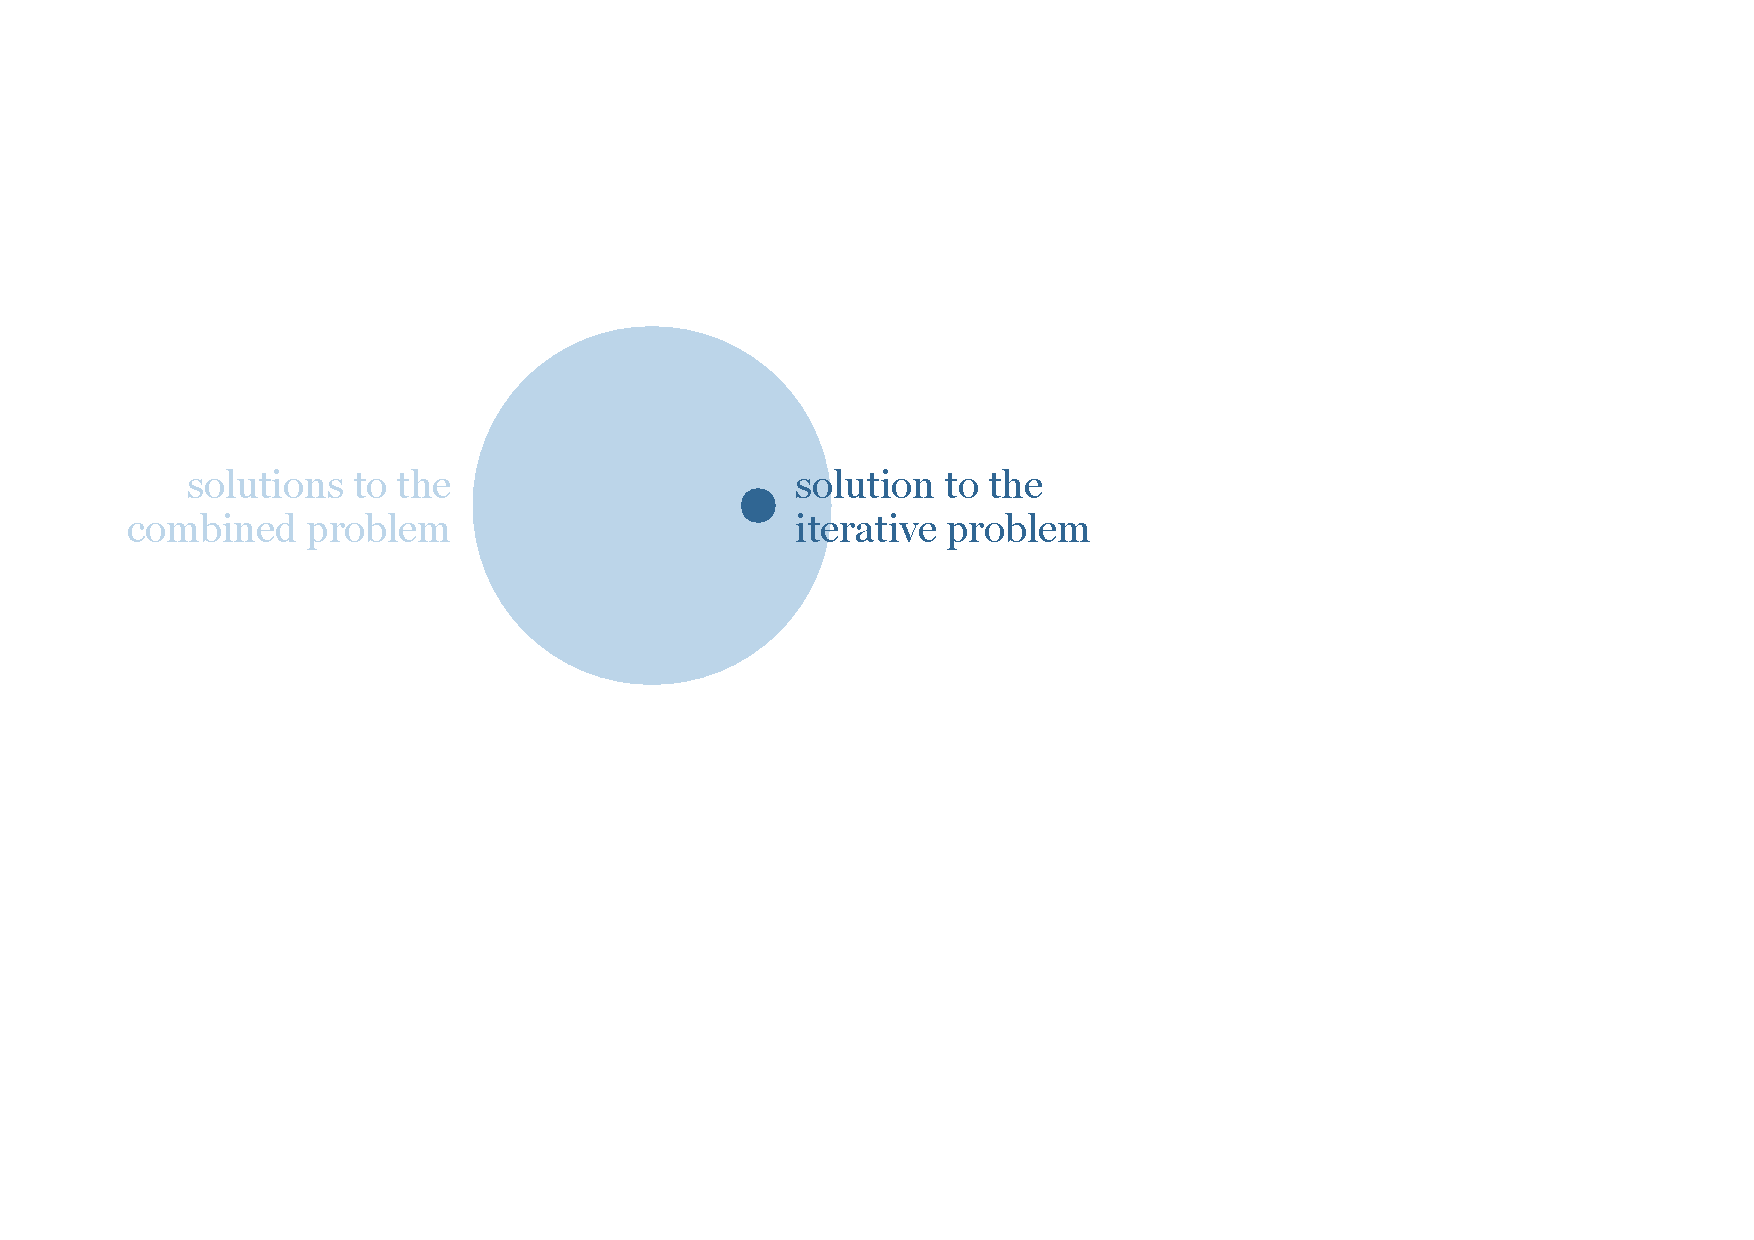
\includegraphics[width=1\textwidth]{./images/pca/venn.pdf}
	}
\end{figure}

%<figure class="narrow">
%<img src="/images/pca/venn.svg" />
%</figure>

\subsection{Characterizing the PCA solution}

Since the eigenvectors are the solution to the PCA problem, you may be forgiven for thinking of the eigenvectors  themselves in terms error minimization or variance maximization. In that case, we should guard against a misconception.

\noindent Look back at the ellipse we drew above. The first eigenvector was the major axis of the ellipse, the direction in which the data bulged out the most. However, the other eigenvector is its \emph{minor} axis. The direction in which the data bulges \emph{the least}, this makes it the direction in which the variance is \emph{minimized}.

\index{Major axis}\index{Minor axis}

To study this a bit more formally, we take the first two proofs of the previous section and turn them around. If we start with the \emph{last} eigenvector and work backward, we are choosing the directions that minimize the variance (and hence maximize the reconstruction error).

\begin{theorem}[Last eigenvector.] The direction in which the variance is minimized, is the eigenvector of \(\bc{\mbA}\) with the smallest eigenvalue.
\end{theorem}
\begin{proof}
 Follow the proof of the \textbf{\gc{first eigenvector}} theorem until the sum
 
\[
\mbz^T\bc{\mbD}\mbz = {z_1}^2 \bc{d}_{11} + \ldots + {z_\bc{m}}^2\bc{d}_\bc{mm} \p
\]

A weighted sum is minimized when all the weight is given to the smallest term. Following the same logic as before, this leads to a one-hot vector \(\hat \mbz = (0, \ldots, 0, 1)\) that selects the last column of \(\rc{\mbP}\), which is the last eigenvector.\hfill\qed
\end{proof}

Did we make a mistake somewhere? We defined the principal components as directions for which variance is maximized. Then we showed that all principal components are eigenvectors. Now we learn that at least one eigenvector actually \emph{minimizes} the variance. What gives?

\index{Variance \emph{mini}mization}

The solution lies in the fact that the sum of all variances is fixed to the sum of the variances of the data, \(z_\text{total}\). Imagine solving the combined problem for \(\rc{k} = \bc{m} - 1\). The resulting variances along the columns of the solution \(\rc{\mbW}\) should be as high as possible. However since all these columns are orthogonal, there is only one direction \(\rc{\mbv}\) left which is orthogonal to all of them. The variance along this direction, \(z_\rc{\mbv}\), is whatever variance we haven't captured in our solution:

\[
z_\rc{1} + \ldots + z_{\bc{m} - 1} + z_\rc{\mbv} = z_\text{total}
\]

Since \(z_\text{total}\) is fixed, maximizing the first \(\bc{m} - 1\) terms is equivalent to minimizing the last. 

We can define a kind of \emph{reverse iterative problem} where we define the last principal component as the direction that minimizes the variance, the last-but-one principal component as the direction orthogonal to the last principal component, the last-but-two principal component as the direction orthogonal to the last two that minimizes the variance and so on. 

\index{Reverse iteration}

We can show that optimizing for this problem gives us exactly the same vectors as optimizing for the original iterative problem which maximized the variance.

\begin{theorem}[Reverse iteration.] Under the reverse iterative problem, the last-but-\(\rc{r}\) principal component chosen coincides with the \(\rc{k}\)-th eigenvector of \(\bc{\mbS}\), with \(\rc{k} = \bc{m} - \rc{r}\), and therefore with the \(\rc{k}\)-th principal component.
\end{theorem}

The proof is the same as that of the \textbf{\gc{PCs as eigenvectors}} theorem, except starting with the smallest eigenvector instead of the largest and choosing \(\hat \mbz\) to \emph{minimize} at every step.

This shows us that it's not quite right to think of the eigenvectors as maximizing or minimizing some quantity like variance or reconstruction error (even though we've defined the principal components that way). The eigenvectors of \(\bc{\mbS}\) simply form a very natural orthonormal basis for the data, from which we can derive natural solutions to optimization objectives in both directions.

There is one question that we haven't answered yet. How do we refine the combined problem so that it coincides with the iterative problem? The one property that we use in our derivations above that is not stated in the combined problem, is that in the new basis, the data are \emph{decorrelated}. If we add this requirement to the optimization objective, we get:

\enlargethispage{3em}

\vspace{-0.5em}
\begin{align*}
\argmax{\rc{\mbW}} & \sum_\gc{i} \left( \mbx_\gc{i}^T\rc{\mbW} \right )^ 2 \\
\text{such that } & \rc{\mbW}^T\rc{\mbW} = \mbI \\
\text{and } & \kc{\frac{1}{N}}\rc{\mbW}^T\mbX^T\mbX\rc{\mbW} \text{ is diagonal.}
\end{align*}

For this problem, there is only one solution (up to negations of the principal components): the PCA solution. With this, we can finally let go of our iterative view of PCA, and embrace methods that compute all principal components in a single operation.


%\section{Conclusion}
 We have come home from a long walk. Let's settle by the fireplace and talk about all the things we've seen. 

We started with a broad idea of PCA as a method that iteratively minimizes the reconstruction error, while projecting into a lower dimensional space. For some reason, we saw last time, this works amazingly well and exposes many meaningful latent dimensions in our data. In this chapter, we showed first that minimizing reconstruction error is equivalent to maximizing variance.

We then looked at eigenvectors, and we show that the eigenvectors of the data covariance \(\bc{\mbS}\) arise naturally when we imagine that our data was originally decorrelated with unit variance in all directions. To me, this provides some intuition for why PCA works so well when it does. We can imagine that our data was constructed by sampling independent latent variables \(\mbz\) and then mixing them up linearly. In our income dataset, in the first chapter, there was one important latent variable: each person's salary. From this, we derived the monthly salary, and the majority of their quarterly income. The other latent variable captured random noise: whether people had some extra income, bonuses, etc.

\begin{figure}[H]
	\centerline{
	\includesvg[width=1\textwidth]{./images/pca/sol-w2.svg}
	}
\end{figure}

%<figure class="narrow">
%<img src="/images/pca/sol-w2.svg" />
%</figure>

We can imagine the same approach with the Olivetti faces. We get \bc{\(4096\)  features}, but under water, most of the work is done by a few \emph{latent} dimensions which are largely independent of each other: the subject's age, the direction of the light source, their apparent gender and so on. All of these can be chosen independently from each other, and are likely mostly decorrelated in the data. That is, if we don't light all women from the left, or only chose old men and young women.
\enlargethispage{13.5pt}

\index{Decorrelation}

\begin{aside}If these assumptions are violated, it may point to undesirable biases in our data. A very relevant topic at the moment. This shows that bias can be defined in terms of the assumed latent variables. Unfortunately, once the data is biased, it reduces our ability to extract the latent features, which makes it more difficult to counteract the bias.
\end{aside}

\index{Bias in data}

Since the assumptions behind our transformation from decorrelated data to the observed data are mostly correct, finding this transformation, and inverting it retrieves the latent dimensions. The greater the variance along a latent dimension, the more variance that particular ``choice'' added to the the data. The choice of the subject's age adds more variance than the lighting, and the lighting adds more variance than the gender.

The heart of the method is the spectral theorem. Without the decomposition \(\bc{\mbS} = \rc{\mbP}\bc{\mbD}\rc{\mbP}^T\), none of this would work. Proving that such a decomposition always exists for a symmetric matrix, and that every matrix for which the decomposition exists is symmetric, is not very difficult, but it takes a lot more background than we had room for here: this includes matrix determinants, the characteristic polynomial and complex numbers. In the next chapter, we will go over all these subjects carefully, building our intuition for them, and finish by thoroughly proving the spectral theorem.

Finally, you may wonder if any of these new insights help us in computing the principal component analysis. The answer is yes, the eigendecomposition \(\bc{\mbS} = \rc{\mbP}\bc{\mbD}\rc{\mbP}^T\) can be computed efficiently, and any linear algebra package allows you to do so. This gives you the principal components \(\rc{\mbP}\), and the rest is just matrix multiplication.

The eigendecomposition is certainly faster and more reliable than the projected gradient descent we've used so far, but it can still be a little numerically unstable. In practice, PCA is almost always computed by \textbf{singular value decomposition} (SVD). The SVD is such a massively useful method that it's worth looking at in more detail. It's inspired very much by everything we've set out above, but its practical applications reach far beyond just the computation of principal components. We'll develop the SVD in Chapter~\ref{chapter:svd} and provide some algorithms for computing both the eigendecomposition and the SVD in Chapter~\ref{chapter:algorithms}. 
But before all that, we'll return to the spectral theorem, and see exactly what is required to prove it.

%\pagebreak
%%\pagestyle{empty}
%~

\cleardoublepage

\chapter{Proving the spectral theorem}
\label{chapter:spectral-theorem}

When I started writing this, it was not meant to be a book. I was going for a short explanation of Principal Component Analysis that was simple, but that also didn't skip any steps. I was frustrated with other explanations that leave things out, or require the reader to take things at face value.

This chapter illustrates why that so often happens. In this chapter we will prove the \textbf{spectral theorem}, which we introduced in the previous chapter. This is very much the dark heart of PCA: the one result from which everything else follows, so it pays to understand it properly. The drawback is that the proof of the spectral theorem adds a boatload of preliminaries to the story.

Suddenly, just to understand this one statement, we need to understand \textbf{determinants}, the \textbf{characteristic polynomial}, \textbf{complex numbers, vectors and matrices} and \textbf{the fundamental theorem of algebra}. All interesting, of course, and worth knowing about, but it's a lot of baggage if you just want to know how PCA works. So I decided to move it all into one self-contained chapter. 

\section{Restating the spectral theorem}

In the last chapter, we learned the following.

An \emph{orthogonal matrix} is a square matrix whose columns are mutually orthogonal unit vectors. Equivalently, an orthogonal matrix is a matrix \(\rc{\mbP}\) for which \(\rc{\mbP}^{-1} = \rc{\mbP}^T\).

\index{orthogonal matrix}

Any square matrix \(\bc{\mbA}\) is \emph{orthogonally diagonalizable} if there exists an orthogonal matrix \(\rc{\mbP}\) and a diagonal matrix \(\bc{\mbD}\) such that \(\bc{\mbA} = \rc{\mbP}\bc{\mbD}\rc{\mbP}^T\). A matrix \(\bc{\mbA}\) is symmetric if \(\bc{\mbA} = \bc{\mbA}^T\).

\index{Orthogonally diagonalizable}

\begin{theorem}[The spectral theorem] A matrix is orthogonally diagonalizable if and only if it is symmetric.
\end{theorem}

\begin{aside}We call this ``the'' spectral theorem in the context of this book. In general, there are many spectral theorems about which operators can be diagonalized under which conditions. 
\end{aside}

Previously, we saw how much follows from this one simple theorem. If we take this to be true, we get eigenvectors, whitening and principal components. 

\index{Spectral theorem}

In the rest of this chapter we'll build a toolkit step by step, with which to analyze this problem. At the end, we'll return to the theorem and apply our tools to prove it.

The first is a very useful function of a matrix: the determinant. 

\vspace{4em}

\section{Determinants}

\index{Determinant of a matrix}

The determinant started life long before linear algebra. As early as the 3rd century BCE, the function was used as a property of a set of linear equations that would allow you to determine whether the equations had a solution.

Later, determinants were studied as functions in their own right. In this context, they were seen as very opaque and abstract: something that was useful in higher mathematics, but hard to explain to the lay person. It wasn't until \emph{matrices} become popular, and in particular the view of a matrix as representing a geometric transformation, that determinants finally acquired an intuitive and simple explanation.

That explanation---apart from some subtleties which we'll discuss later---is that for a square matrix \(\bc{\mbA}\), thre determinant expresses how much \(\bc{\mbA}\) \emph{inflates} the space it transforms.

For example, here are three different ways that a matrix might transform space to squish and stretch in different directions.

\begin{figure}[H]
	\centerline{
	\includegraphics[width=1\textwidth]{./images/pca-3/mona-lisa.pdf}
	}
	\caption*{Three linear transformations, showing the effect on the Mona Lisa, and the \bc{unit square}.}
\end{figure}

%<figure class="narrow">
%<img src="/images/pca-3/mona-lisa.svg" />
%<figcaption>
%Three linear transformations, showing the effect on the Mona Lisa, and the <span class="bc">unit square</span>.
%</figcaption>
%</figure>

In the first, everything is stretched equally in all directions by a factor of \(2\). That means that a square with area \(1\) in the original (a \emph{unit} square) has area \(4\) after the transformation by \(\bc{\mbA}\) (since both its sides are doubled). This is what we mean by inflating space: the determinant of \(\bc{\mbA}\) is 4 because transforming something by \(\bc{\mbA}\) increases its area by a factor of 4. In the second example, We stretch by \(1.1\) in one direction, and shrink to \(0.5\) in the other. The result is that that a unit square in the original ends up smaller after the transformation: the determinant of \(\bc{\mbB}\) is \(0.5 \times 1.1 = 0.55\).

\begin{aside}To see that objects other than squares are inflated by the same amount, just subdivide it into small squares. Each of the squares is inflated by the same amount, so the total is as well.
\end{aside}

The third example is a little trickier. The Mona Lisa is again squished and stretched in different directions, but these are not aligned with the axes. The area of the unit square seems to be getting a little smaller, but how can we tell by how much exactly?

Before we dig into the technical details, let's first look at why it is worth doing so. Why is it so important to know by how much a matrix inflates space? There are many answers, but in the context of this series, the most important reason to care about the determinant is that it gives us a very convenient characterization of \emph{invertible matrices}.

\noindent An invertible matrix is simply a matrix whose transformation is invertible. That is, after we apply the transformation \(\mby \leftarrow \bc{\mbA}\mbx\) we can always transform \(\mby\) back to \(\mbx\), and end up where we started. 

When is a matrix not invertible? When multiple inputs \(\mbx\) are mapped to a single output \(\mby\). In linear transformations, this happens when the input is squished so much in one direction, that the resulting space has a lower dimensionality than the original.

\begin{figure}[H]
	\centerline{
	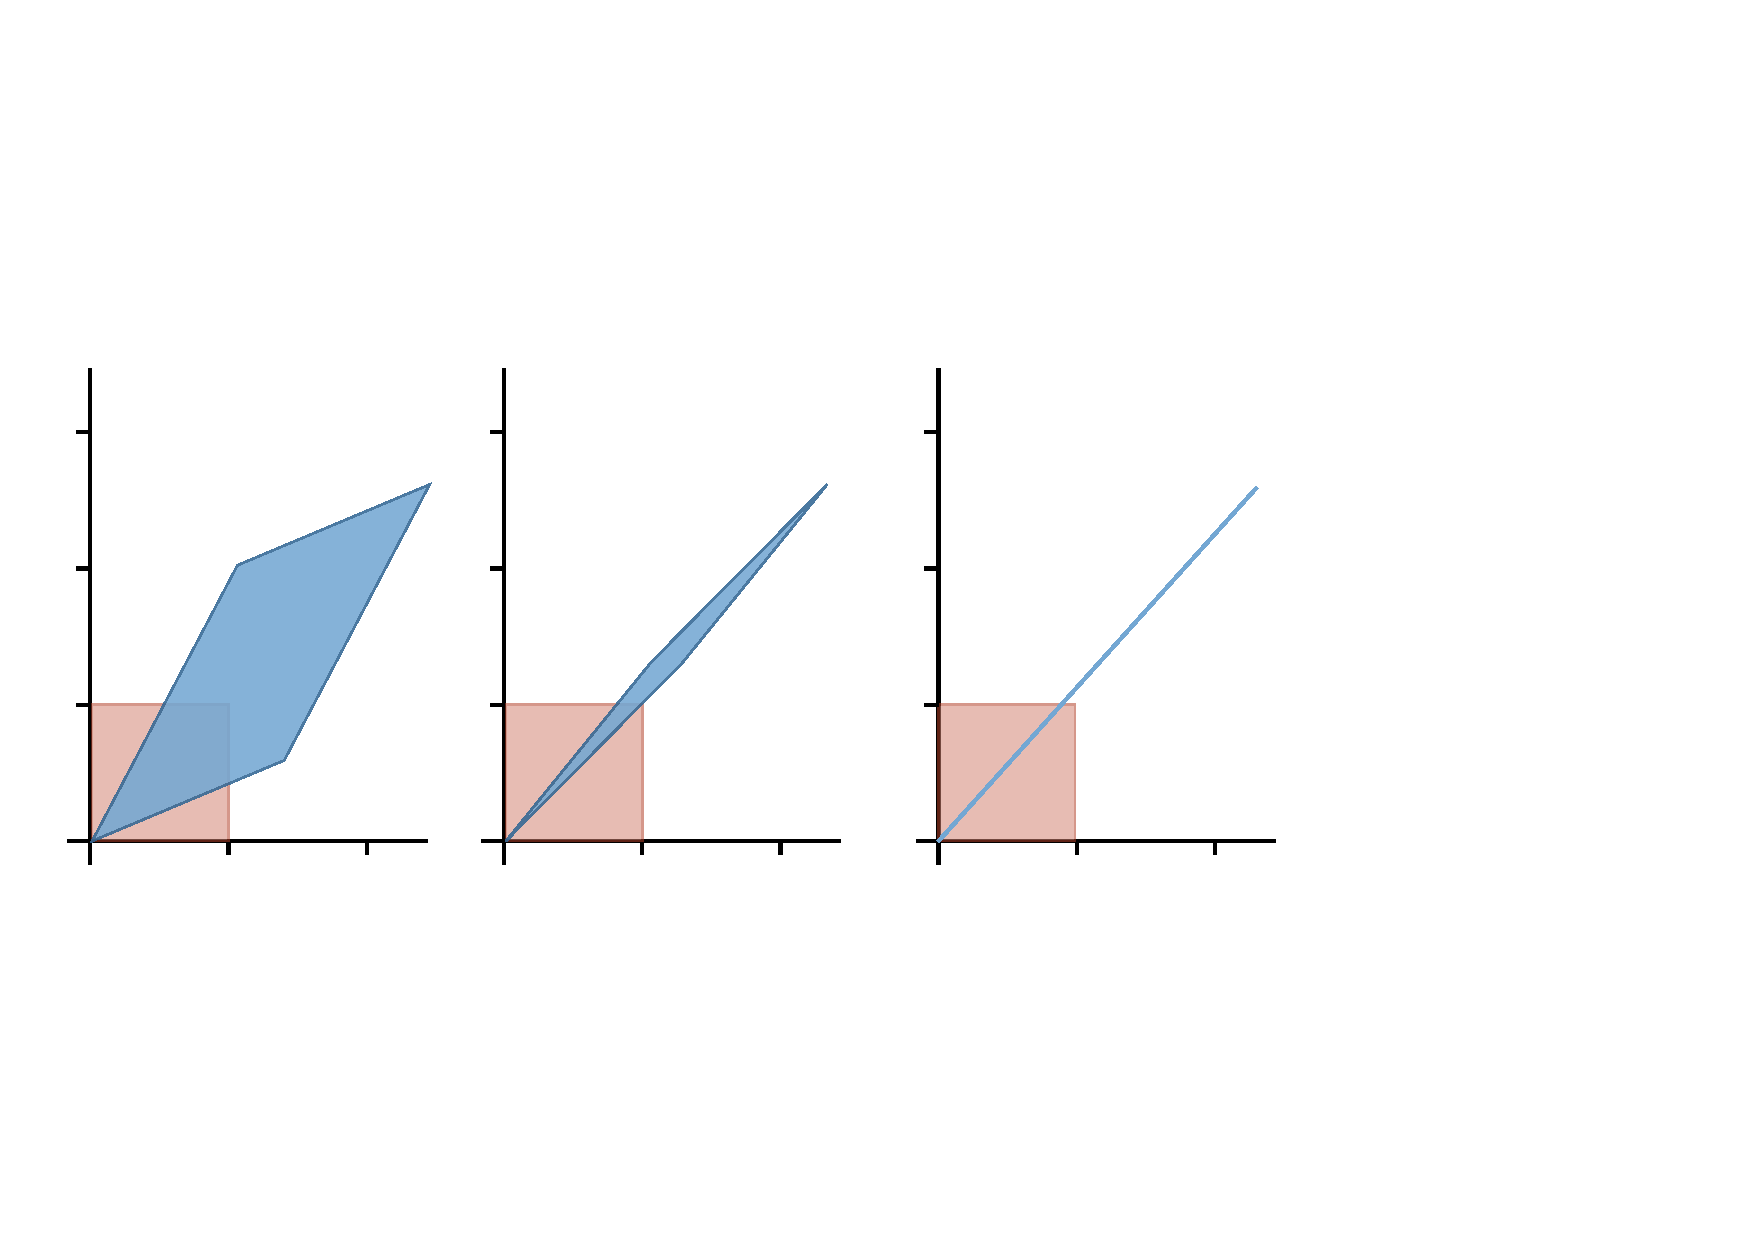
\includegraphics[width=1.2\textwidth]{./images/pca-3/invertible.pdf}
	}
	\caption*{Three transformations with increasingly small determinant. In the third, the unit square is squeezed into a line. Note that the two edges on the bottom left of the square are mapped to the same part of the line, so the transformation is not invertible. }
\end{figure}

%<figure class="narrow">
%<img src="/images/pca-3/invertible.svg" />
%<figcaption>Three transformations with increasingly small determinant. In the third, the unit square is squeezed into a line. Note that the two edges on the bottom left of the square are mapped to the same part of the line, so the transformation is not invertible. 
%</figcaption>
%</figure>

We don't need to know how to compute the determinant to know what its value is in this case. The unit square is mapped to a line segment, so its area goes from \(1\) to \(0\). This is how the determinant helps us to characterize invertible matrices: if the determinant is non-zero, the matrix is invertible, if the determinant is zero, the matrix is not invertible, or \emph{singular}. 

\index{Singular matrices}\index{Invertible matrices}

\subsection{Computing the \(2\times 2\) determinant}

Using this definition, it's pretty straightforward to work out what the formula is for the determinant of a matrix \(\bc{\mbA}\) that transforms a 2D space. We'll start by drawing a unit square, and labeling the four corners:

\begin{figure}[H]
	\centerline{
	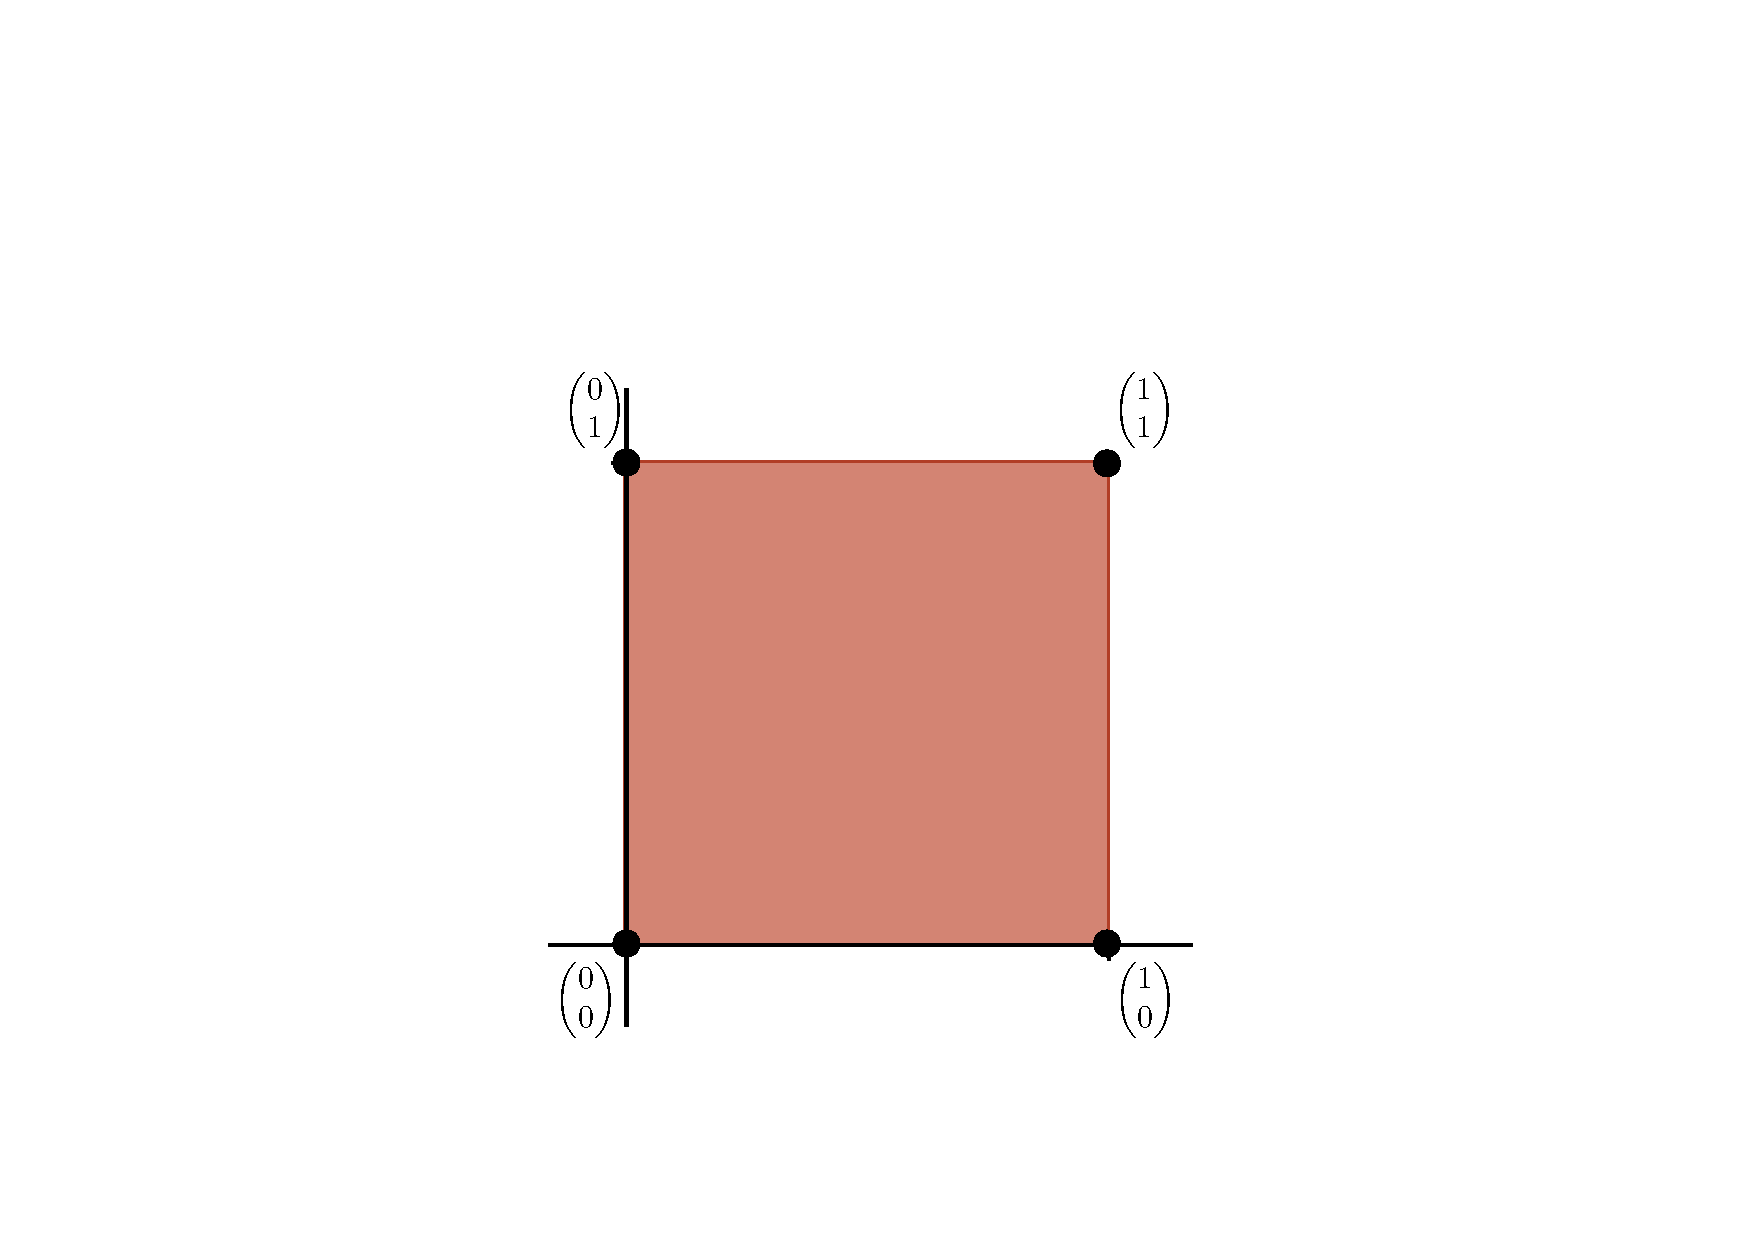
\includegraphics[width=0.4\textwidth]{./images/pca-3/corners.pdf}
	}
\end{figure}

%<figure class="fourth center">
%<img src="/images/pca-3/corners.svg" />
%</figure>

The corner points \((0,0)\), \((0,1)\) \((1,0)\) and \((1,1)\) can be transformed by multiplying them by \(\bc{\mbA}\). we know that under a linear operation like this, line segments stay line segments, so the four edges of the square are transformed to line segments, and the resulting figure between the four points must be a quadrilateral. We also know that \emph{parallelism is preserved}: two line segments that were parallel before the transformation are parallel after. Lastly, we know that the origin stays where it is, unless we apply a translation, so corner \((0, 0)\) is not affected by the transformation. All this means that the picture after the transformation will look something like this.

\begin{figure}[H]
	\centerline{
	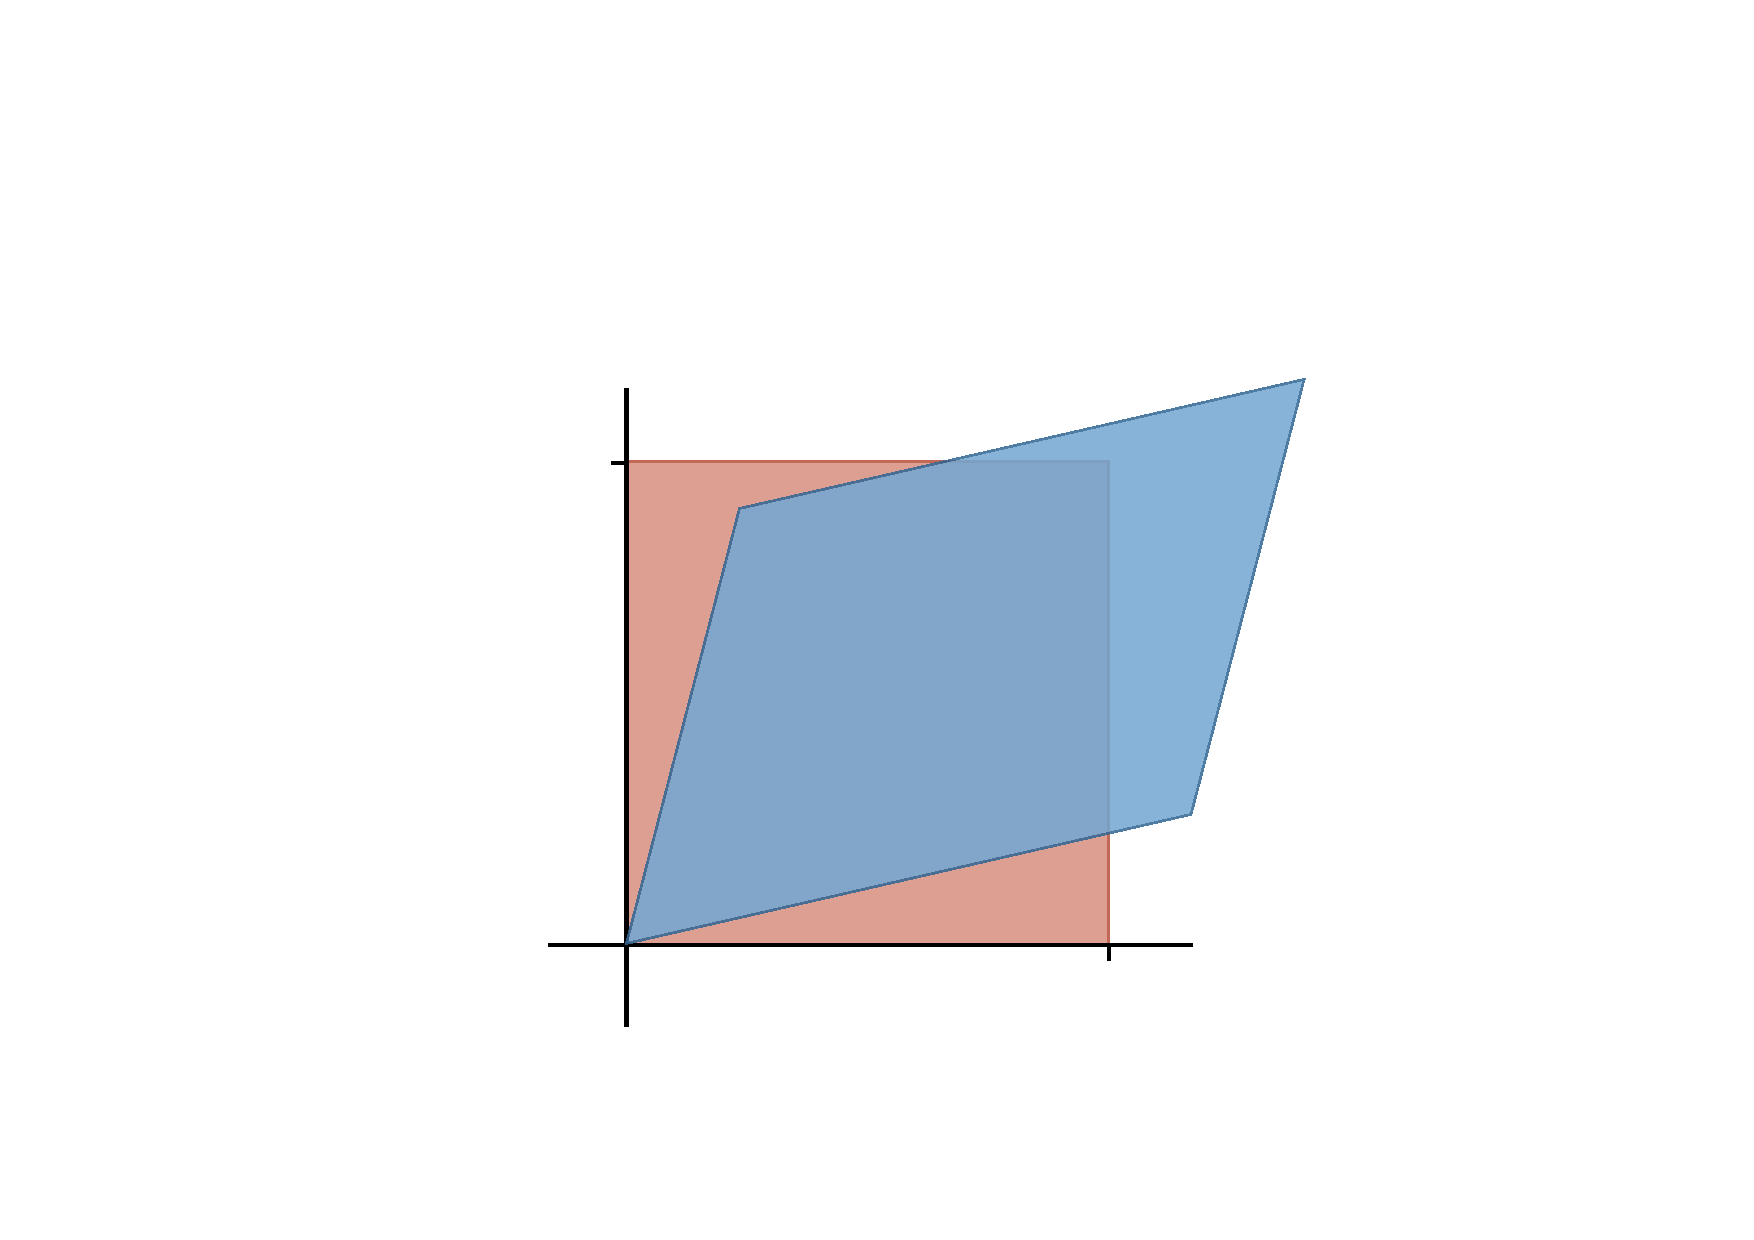
\includegraphics[width=0.6\textwidth]{./images/pca-3/pgram.pdf}
	}
\end{figure}
%<figure class="fourth center">
%<img src="/images/pca-3/pgram.svg" />
%</figure>

A parallelogram with one corner touching the origin. The determinant tells us the ratio between the area of \bc{the paralellogram} and \rc{the original square}. Since the original square has area \(1\), the area of the parallelogram is the determinant of \(\bc{\mbA}\). 

Working this out requires only a small amount of basic geometry. Here's the simplest way to do it.

We first name the four elements of our matrix:

\[
\bc{\mbA} = \begin{pmatrix} a & b \\ c & d \end{pmatrix}
\]

We can now name the four corners of our parallelogram in terms of these four scalars, by multiplying the corner points of the unit square by \(\bc{\mbA}\):

\[
\begin{matrix}
\times
& \begin{pmatrix}0\\ 0\end{pmatrix}
& \begin{pmatrix}1\\ 0\end{pmatrix} 
& \begin{pmatrix}0\\ 1\end{pmatrix} 
& \begin{pmatrix}1\\ 1\end{pmatrix} 
\\
\bc{\begin{pmatrix} a & b \\ c & d \end{pmatrix}}
& \begin{pmatrix}0\\ 0\end{pmatrix}
& \begin{pmatrix}a\\ c\end{pmatrix}
& \begin{pmatrix}b\\ d\end{pmatrix}
& \begin{pmatrix}a+b\\ c+d\end{pmatrix}
 \\
\end{matrix}
\]

This gives us the following picture.

\begin{figure}[H]
	\centerline{
	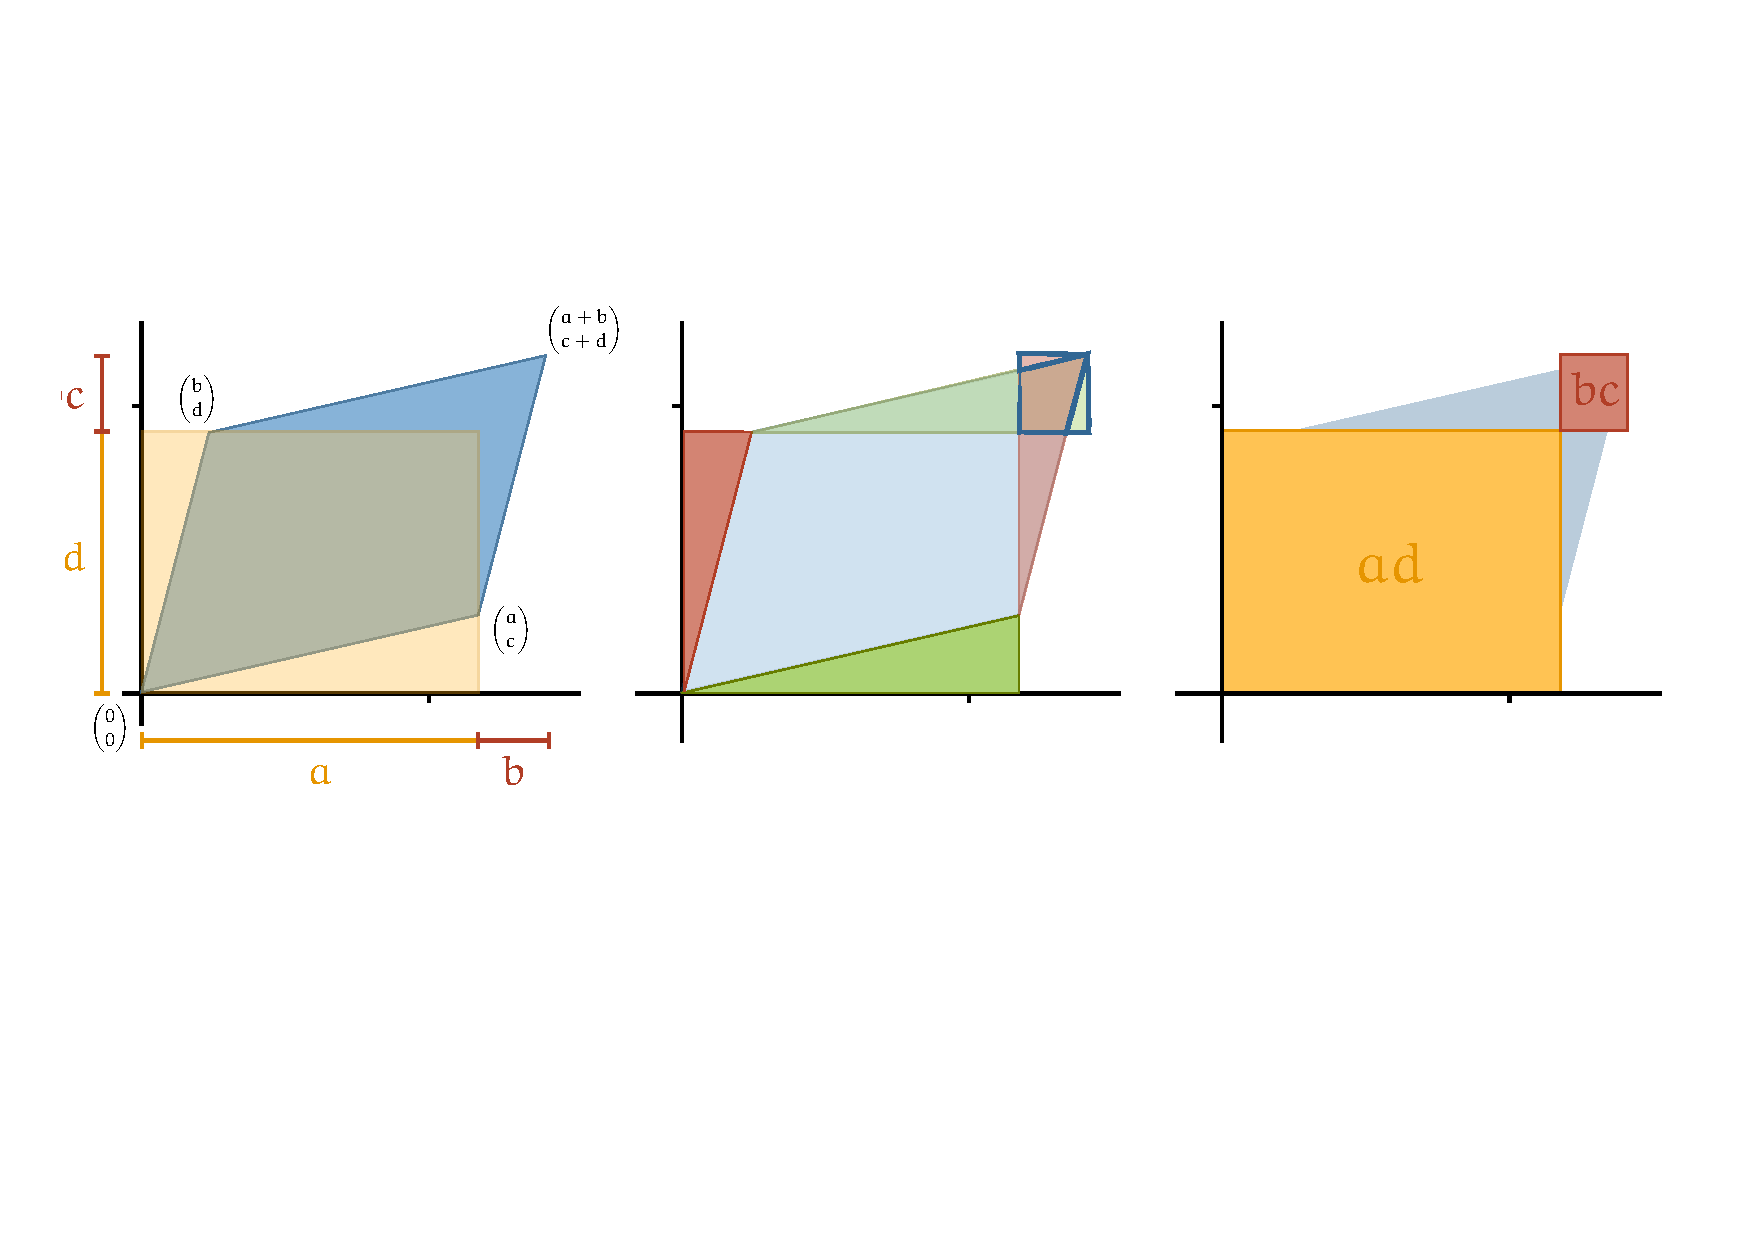
\includegraphics[width=1.3\textwidth]{./images/pca-3/geometric.pdf}
	}
\end{figure}
%<figure class="wide centering">
%<img src="/images/pca-3/geometric.svg" class="own-size"/>
%</figure>

Here we can see the area of the paralellogram clearly: there is one \oc{large rectangle} of area \(\oc{ad}\). To get from this area to the area of our parallelogram, we should subtract the area of the green triangle in the bottom, which is part of the rectangle but not the parallelogram. 

But then, there's a green triangle at the top, with the same size, which is (mostly) part of the parallelogram but not of the rectangle, so these cancel each other out. We follow the same logic for the red triangles.

Putting all this together, the rectangle with area \(\oc{ad}\) has the same area as the parallellogram, except that we are overcounting three elements (outlined in blue): the two small triangles in the box at the top, which are not part of the paralellogram, and the overlap between the green and the red triangles, which we've counted twice. These three overcounted elements  add up precisely to the box at the top-right, which has area \(\rc{bc}\). 

So, the area of the paralellogram, and therefore the determinant of the matrix \(\bc{\mbA}\) is \(\oc{ad} - \rc{bc}\). Or, in words: the determinant of a \(2 \times 2\) matrix is the diagonal product minus the antidiagonal product. 

%\begin{aside}
%If you don't trust such visual proofs, here it is algebraically:
%\begin{align*}
%\text{det}\;\bc{\mbA} + 2\left (\tfrac{1}{2}ac + \tfrac{1}{2}bd 2bc\right ) &= (a + b)(b + d)\\
%\text{det}\;\bc{\mbA} + \kc{ac} + \kc{bd} + 2bc &= \kc{ac} + ad + bc + \kc{bd}\\
%\text{det}\;\bc{\mbA} &= ad - bc
%\end{align*}
%\end{aside}

We will write the determinant of a matrix \(\bc{\mbA}\) with two vertical bars around the matrix. When we write out the values of the matrix explicitly, we will remove the matrix parentheses for clarity:

\[
|\bc{\mbA}| = \left |\, \begin{matrix} \oc{a} & \rc{b} \\ \rc{c} & \oc{d} \end{matrix} \;\right | = \oc{ad} - \rc{bc} \p
\]

\subsection{Negative determinants}

\index{Determinant!Negative-valued}

In the picture we drew to derive this, \(ad\) was bigger than \(bc\), so the determinant was positive. But this is not guaranteed. Look at the two column vectors of our matrix. If we flip them around then the determinant becomes:

\[
\left |\,\begin{matrix} \rc{b}  & \oc{a} \\ \oc{d} & \rc{c} \end{matrix}\; \right | = \rc{bc} - \oc{da} \p
\]

Assuming the values in the matrix are the same, this is the same quantity as before, but negative. Areas can't be negative, so how do we interpret this?

The magnitude remains the same, so the simplest solution is just to adjust our definitions: \emph{the absolute value} of \(|\bc{\mbA}|\) is the amount by which \(\bc{\mbA}\) inflates space.

However, in many situations, the idea of a ``negative area'' actually makes a lot of sense. Consider, for instance, this graph of the velocity of a train along a straight track from one station to another and back again:

\index{Negative area}\index{Signed area}

\begin{figure}[H]
	\centerline{
	\hspace{-0.9cm}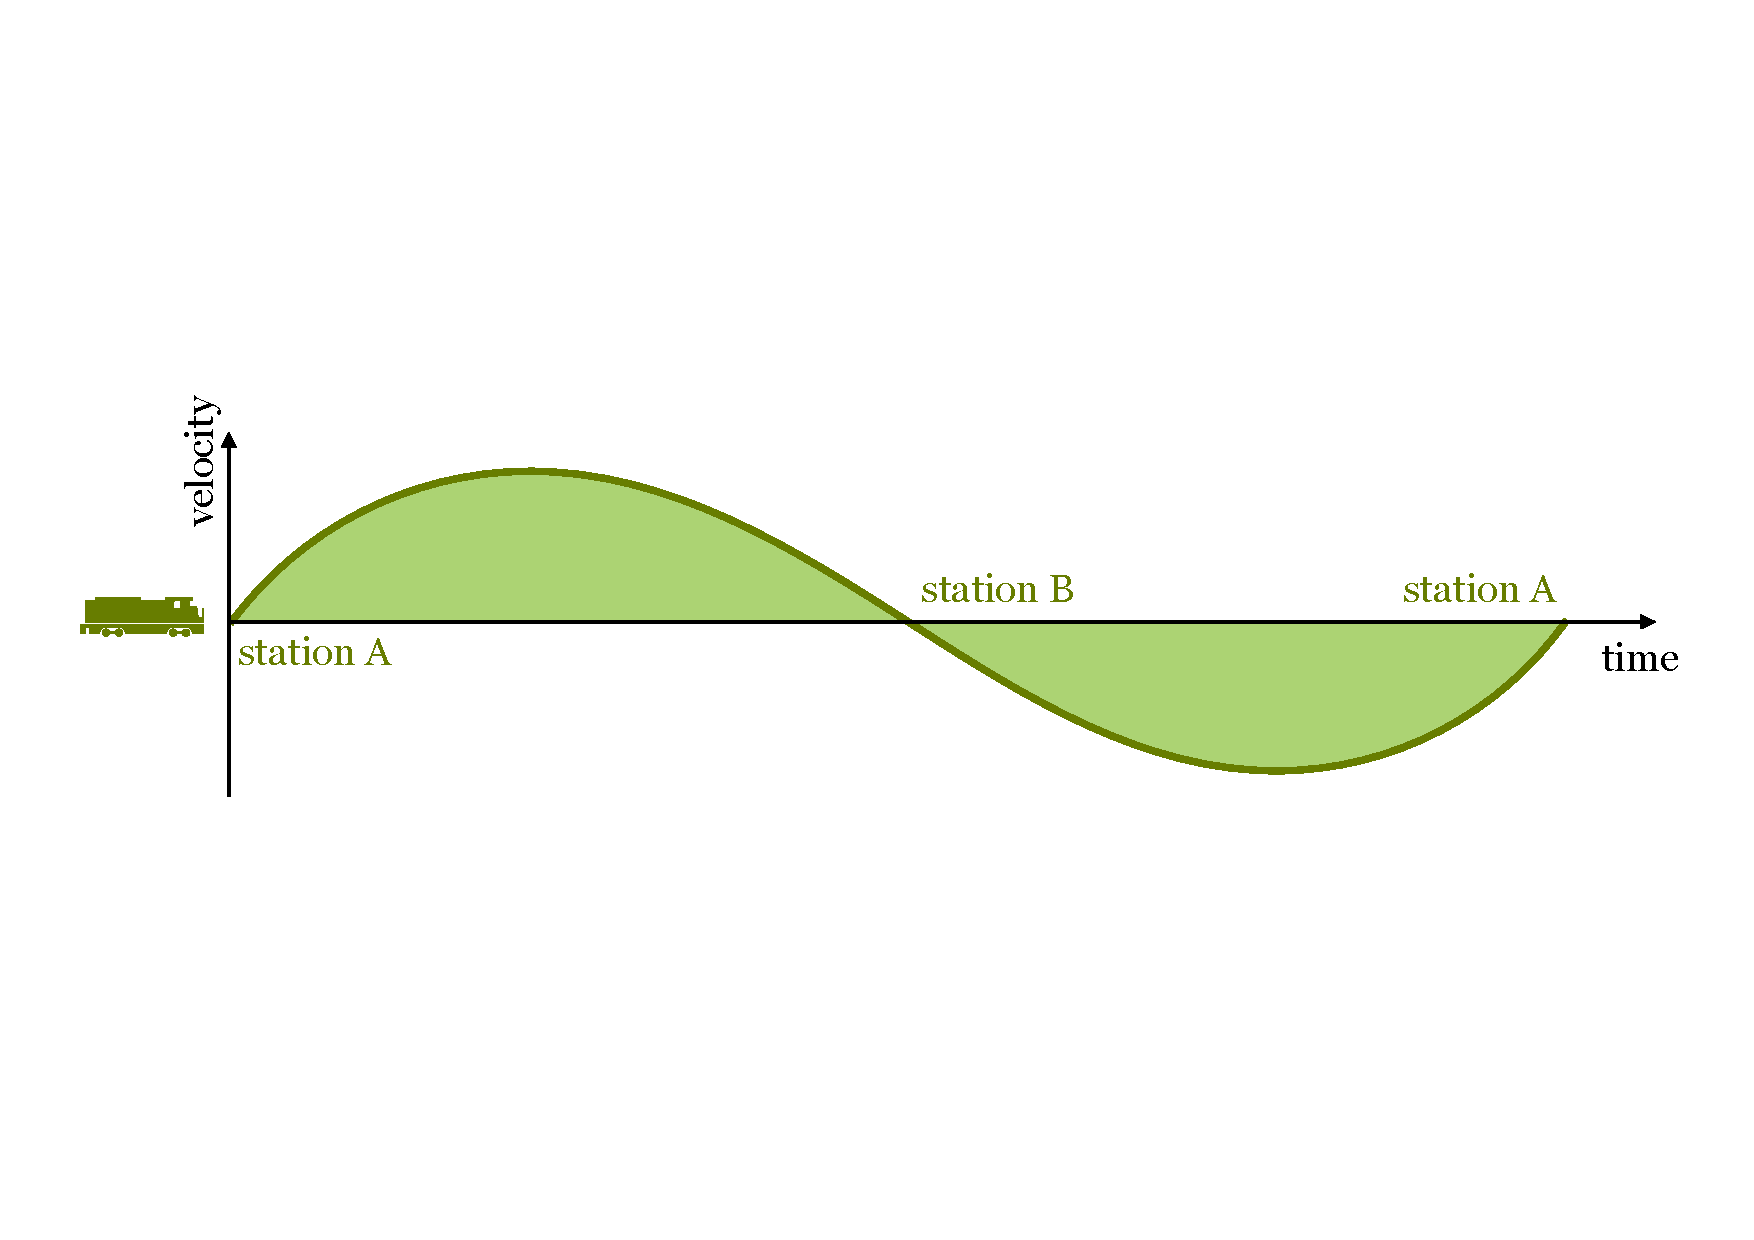
\includegraphics[width=1.1\textwidth]{./images/pca-3/train.pdf}
	}
\end{figure}
%<figure class="narrow">
%<img src="/images/pca-3/train.svg" />
%</figure>

Here, we've used a negative velocity to represent the train traveling backwards. If you've done some physics, then you'll know that the area under the speed curve represents distance traveled. Here we have two options: we can look at the absolute value of the area, and see that the train has, in total, travelled twice the distance between the stations. We can also take areas below the horizontal axis to be \emph{negative}. Then, their sum tells us that the total distance between the train's starting point and its final position is exactly zero.

All this is just to say, if you need positive areas, just take the magnitude of the determinant, but don't be too quick to throw away the sign. It may have some important meaning in your particular setting. For our purposes, we'll need these kinds of areas when we want to think about determinants for larger matrices.

We'll call this kind of positive or negative area a \emph{signed area}, or signed \emph{volume} in higher dimensions. You can think of the parallelogram as a piece of paper. If \(\bc{\mbA}\) stretches the paper, but doesn't flip it around, the singed area is positive. If the paper is flipped around, so that we see the reverse, the area is negative. If you flip the paper around twice, the sign becomes positive again.

\index{Signed volume}

\subsection{Towards \(n \times n\) determinants}

Let's think about what we'll need to generalize this idea to \(3 \times 3\) matrices and beyond, to general \(n \times n\) matrices. The basic intuition generalizes: we can start with a unit (hyper)cube in \(n\) dimensions. A square matrix transforms this into an analogue of a parallelogram, called a parallellotope. 

For a given dimensionality we can define a notion of \(n\)-volume. The 3-volume is simply the volume we already know. The \(n\)-volume of an n-dimensional ``brick'', the analogue of a rectangle, is the product of its extent in each direction: height times width times length and so on in all directions. This means that the unit hypercube, which has sides of length 1 in all directions, always has \(n\)-volume 1.

We will assume, by analogy with the \(2 \times 2\) case, that the determinant of an \(n \times n\) matrix \(\bc{\mbA}\) is the \(n\)-volume of the parallellotope that results when we transform the unit hypercube by \(\bc{\mbA}\). 

\begin{aside}Note that there are \(3 \times 3\) matrices that will flatten the unit cube into a parallelogram. In this case, we are \textbf{not} interested in the \emph{area} of the parallelogram as we were before. The matrix is \(3 \times 3\), so we care about the resulting \emph{volume}, which in such cases would be \(0\).
\end{aside}

We can generalize a few useful properties from the \(2 \times 2\) case. The columns of \(\bc{\mbA}\) are those vectors that describe the edges that touch the origin. We'll call these the \textbf{basis vectors} of the parallelogram/-tope.

\enlargethispage{3em}

\begin{figure}[H]
	\centerline{
	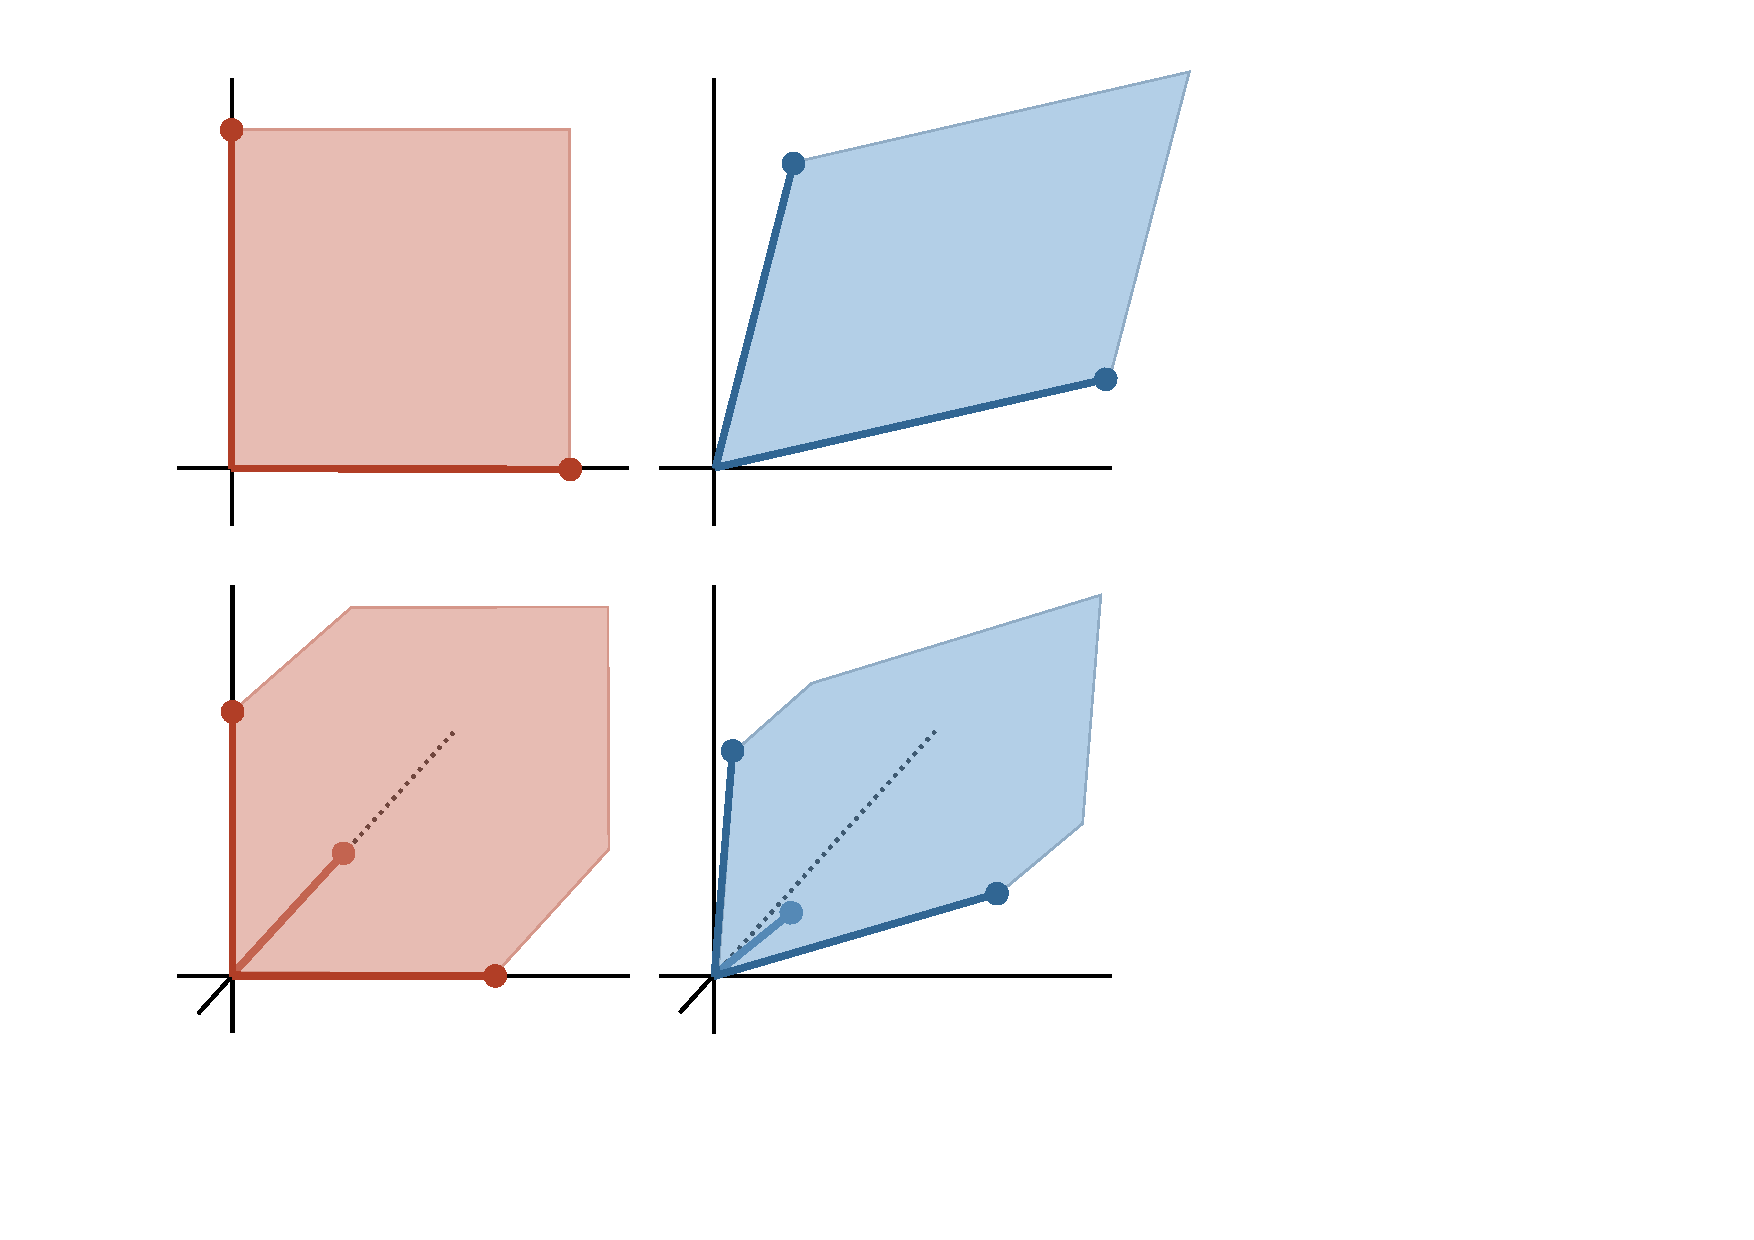
\includegraphics[width=0.8\textwidth]{./images/pca-3/basis-vectors.pdf}
	}
	\caption*{The edges of the \rc{unit cube} that touch the origin are the standard basis vectors. These are mapped to the edges of the \bc{parallelotope} that touch the origin. These are the column vectors of \(\bc{\mbA}\). We call these the \emph{basis vectors of the parallelotope}.
}
\end{figure}

%<figure class="narrow">
%<img src="/images/pca-3/basis-vectors.svg" />
%<figcaption>The edges of the <span class="rc">unit cube</span> that touch the origin are the standard basis vectors. These are mapped to the edges of the <span class="bc">parallelotope</span> that touch the origin. These are the column vectors of \(\bc{\A}\). We call these the <em>basis vectors of the parallelotope</em>.
%</figcaption>
%</figure>

The proof we gave for the \(2 \times 2\) determinant is very neat, but it isn't very easy to generalize to the \(n \times n\) case in an intuitive way.

%<!-- 
%<aside>It's not easy, but it is possible, if you use the idea that any two shapes that tile space with the same periodicity have the same volume. Here is <a href="https://math.stackexchange.com/a/2509560/24168">a StackExchange post that details this</a>. As neat as this is, it's a little involved for our purposes.
%</aside>
% -->

Instead, let's re-prove our result for the \(2 \times 2\) case in a way that's easier to generalize. We'll need to convince ourselves of three properties of the area of a parallellogram.

\begin{aside}These are not difficult to prove, but we'll focus here on the geometric intuition. If you want a more rigorous proof, it's easier to let this intuition go, and work purely symbolically.
\end{aside}

The \textbf{first property} we need is that if we move one of the sides of the parallelogram without changing its direction, the area of the parallellogram remains the same. This is easy to see visually.

\begin{figure}[H]
	\centerline{
	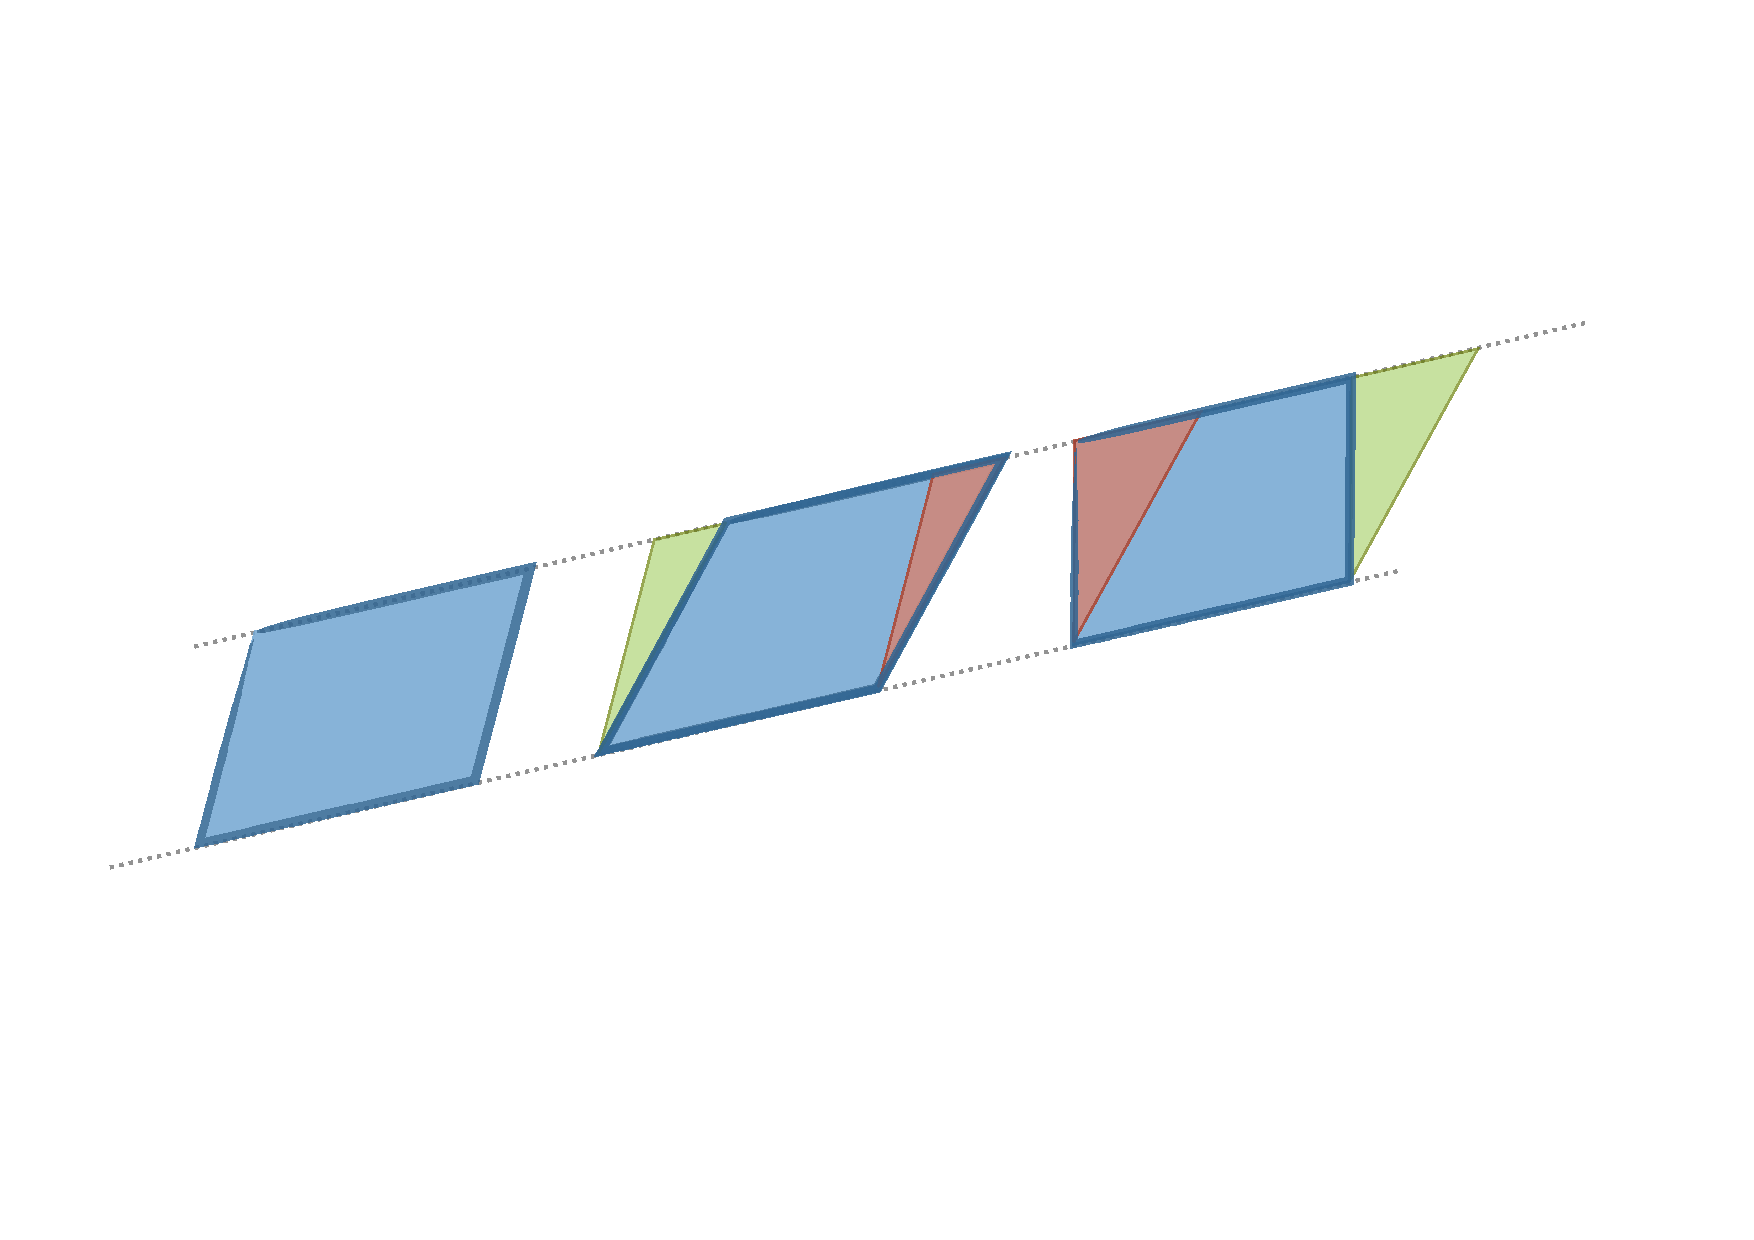
\includegraphics[width=1\textwidth]{./images/pca-3/skew.pdf}
	}
	\caption*{A skew transformation preserves the area of a parallelogram. This means we can align one of the edges with the axes without changing the area.
	}
\end{figure}

%<figure class="narrow">
%<img src="/images/pca-3/skew.svg" />
%<figcaption>A skew transformation preserves the area of a parallelogram. This means we can align one of the edges with the axes without changing the area.
%</figcaption>
%</figure>

Note that shifting one of the sides always \rc{adds a triangle} to the parallellogram and \gc{takes away} a triangle of the same size, so the total stays the same. The last example is particularly relevant: we can shift the parallelogram so that one of its edges is aligned with one of the axes. If we do this twice, we'll have a \emph{rectangle} with an area equal to that of the original parallellogram.

\enlargethispage{2em}

What does this look like in the original matrix? Remember that the columns of the matrix are the two edges of the parallelogram that touch the origin. Shifting one of them in this way is equivalent to adding or subtracting a small multiple of the other to it.

\begin{figure}[H]
	\centerline{
	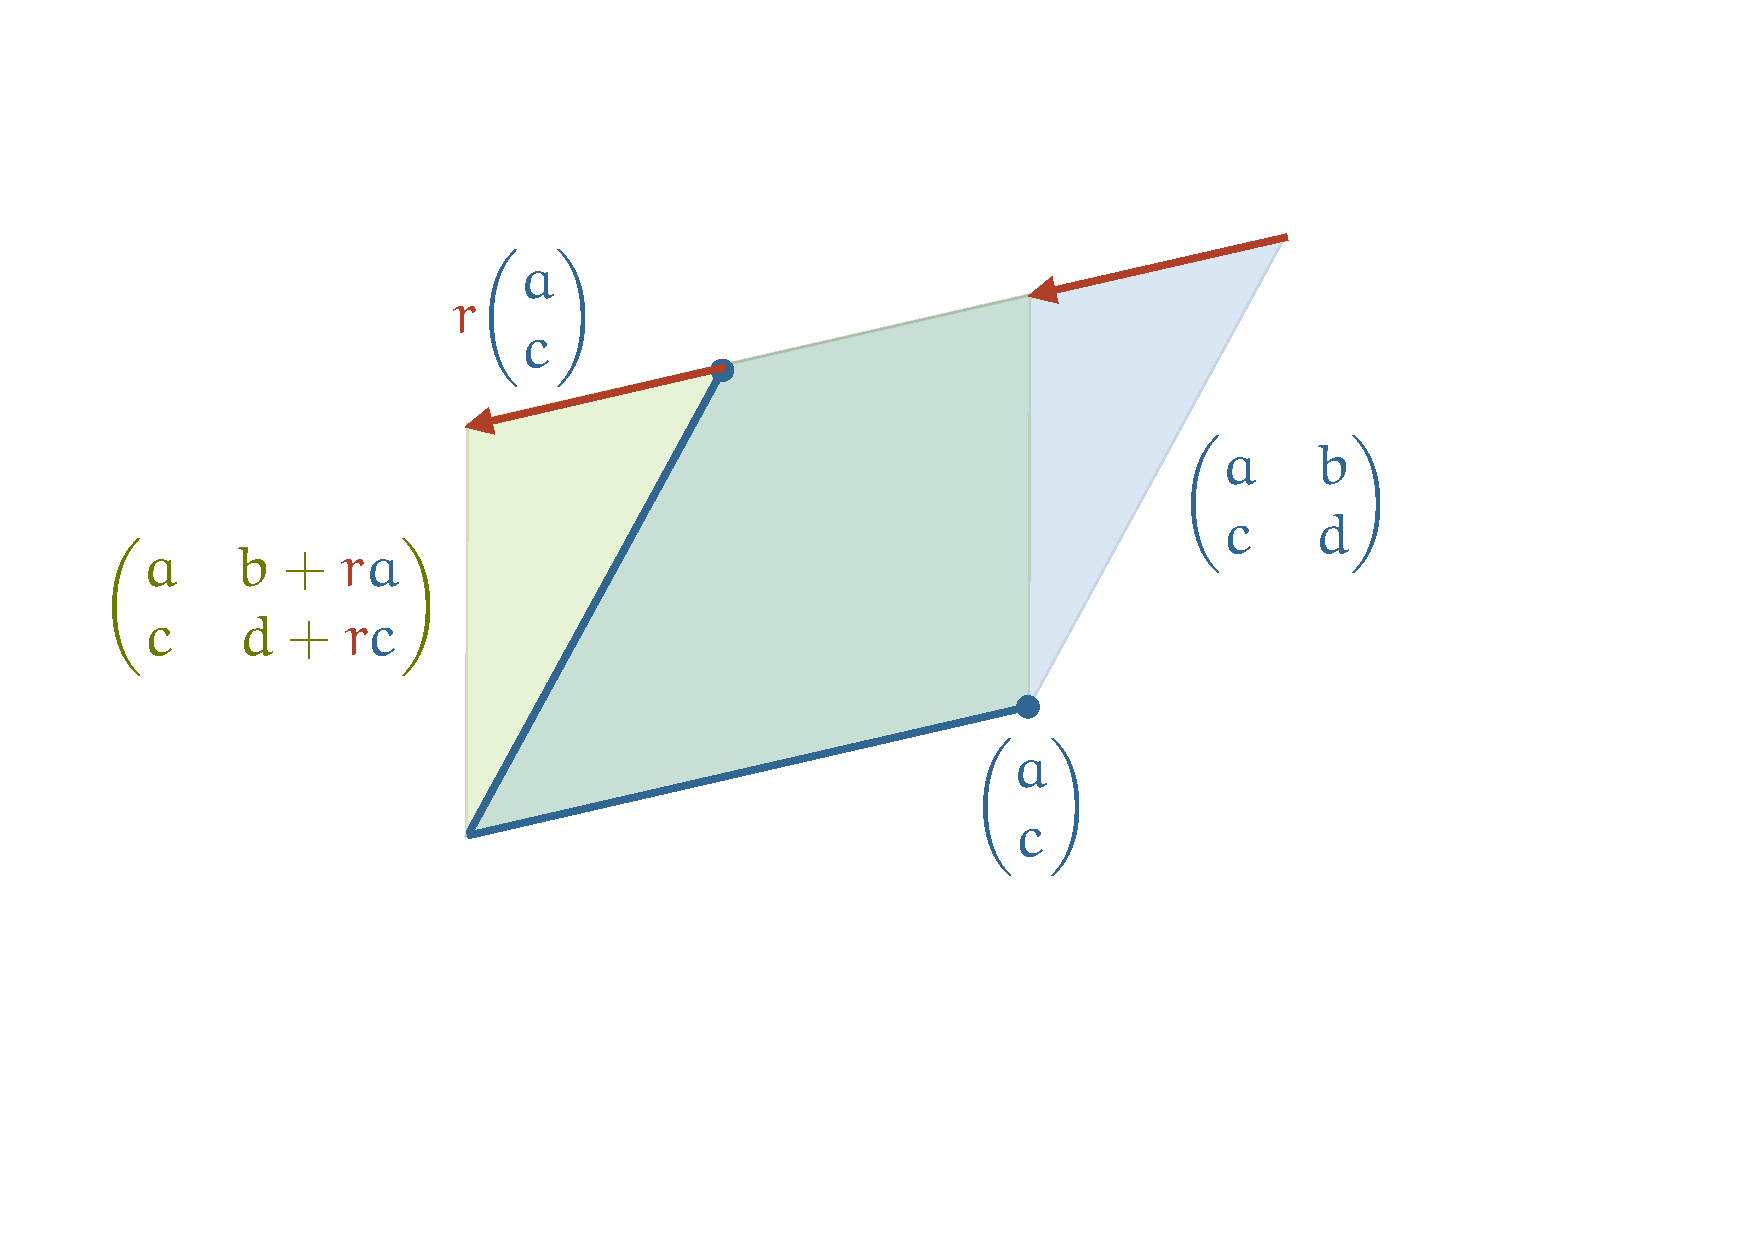
\includegraphics[width=1\textwidth]{./images/pca-3/align.pdf}
	}
	\caption*{To axis-align a parallellogram defined by a matrix, we take one of the columns, and add or subtract some multiple of the other column.
	}
\end{figure}

%<figure class="narrow">
%<img src="/images/pca-3/align.svg" />
%<figcaption>To axis-align a parallellogram defined by a matrix, we take one of the columns, and add or subtract some multiple of the other column.
%</figcaption>
%</figure>

That is, if we take one of the columns of \(\bc{\mbA}\), multiply it by any \rc{non-zero scalar}, and add it to another column, the area of the resulting parallelogram is unchanged. If we name the column vectors \(\bc{\mbv}\) and \(\bc{\mbw}\), and write \(|\,\bc{\mbv}, \bc{\mbw}\,|\) for the determinant of the matrix with these column vectors, then we have

\[
|\,\bc{\mbv}, \bc{\mbw}\,| = |\,\bc{\mbv} + \rc{r}\bc{\mbw}, \bc{\mbw}\,| \;\;\text{for any nonzero \(\rc{r}\).}
\]

This kind of transformation is called a skew or a shear, so we'll call this property \textbf{skew invariance}: the area of a parallelogram is skew invariant. 

\index{Skew transformation}\index{Shear transformation}\index{Skew invariance|textbf}

The \textbf{second property} we need, is that if we take one of the column vectors of the matrix, say \(\bc{\mbv}\), and write it as the sum of two other vectors \(\bc{\mbv} = \oc{\mbv}^1 + \oc{\mbv}^2\), then the area of the paralellogram made by basis vectors \(\bc{\mbv}, \bc{\mbw}\) is the sum of the area of the two smaller parallelograms with basis vectors \(\oc{\mbv}^1, \bc{\mbw}\) and \(\oc{\mbv}^2, \bc{\mbw}\) respectively.

This is easy enough to see if \(\oc{\mbv}^1\) and \(\oc{\mbv}^2\) point in the same direction. Then the two smaller parallelograms together simply combine to form the larger one.

If they don't point in the same direction, we can skew them until they do. Since we've already shown that the area is skew invariant, none of this changes the area of the paralellogram.

\begin{figure}[H]
	\centerline{
	\hspace{1em}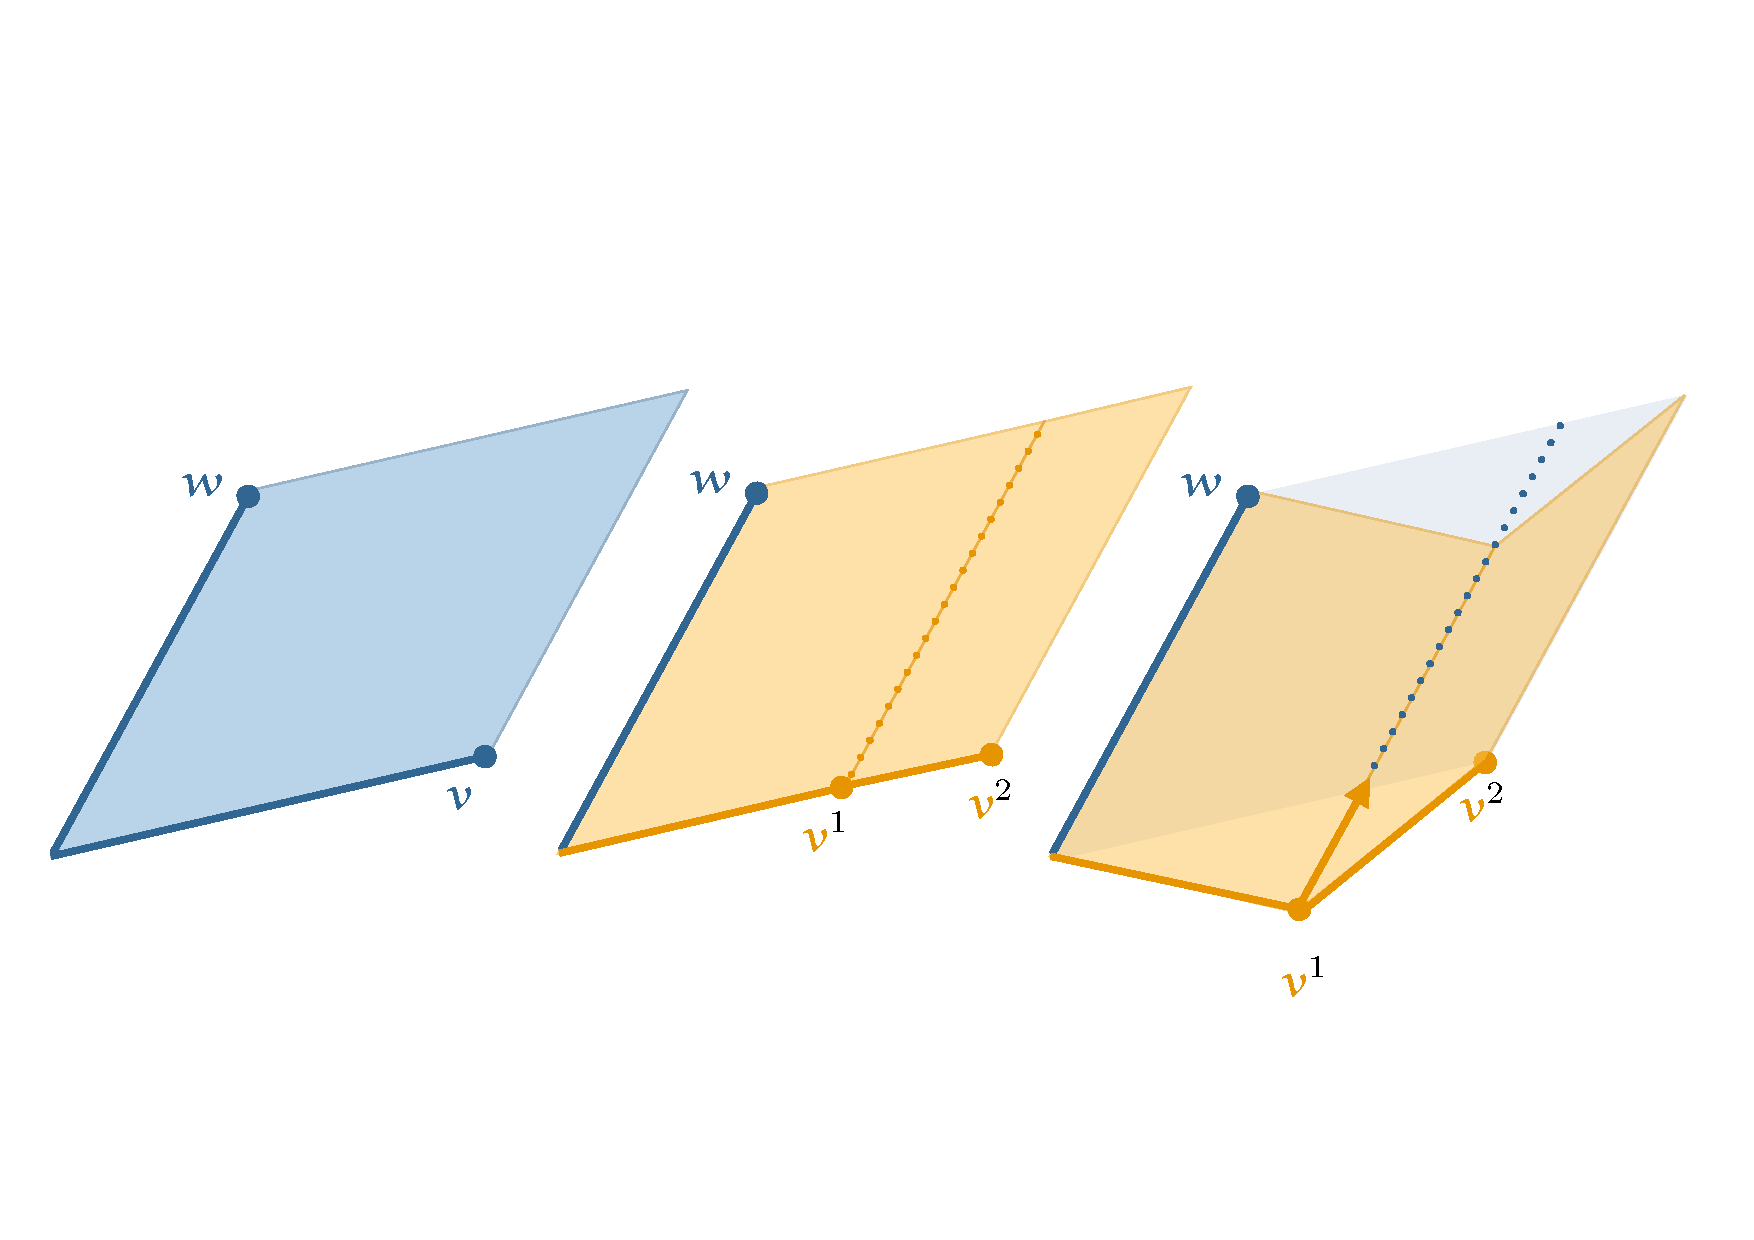
\includegraphics[width=1.2\textwidth]{./images/pca-3/sum.pdf}
	}
	\caption*{If we break one of the basis vectors into the sum of two other vectors, the original area is the sum of the two parts. This is easy to see if the sub-vectors point in the same direction as the original. If they don't, we simply skew them until they do.
	}
\end{figure}

%<figure class="narrow">
%<img src="/images/pca-3/sum.svg" />
%<figcaption>If we break one of the basis vectors into the sum of two other vectors, the original area is the sum of the two parts. This is easy to see if the sub-vectors point in the same direction as the original. If they don't, we simply skew them until they do.
%</figcaption>
%</figure>

Symbolically, this means that if we break one of the vectors in a matrix into a sum of two other vectors, then the determinant distributes over that sum:

\[
|\;\oc{\mbv}^1 + \oc{\mbv}^2, \bc{\mbw}\;| = |\;\oc{\mbv}^1, \bc{\mbw}\;| + |\;\oc{\mbv}^2, \bc{\mbw}\;| \p
\]

We won't need it here, but we can also show that multiplying one of the vectors by some scalar scales the determinant by the same value. These two properties together are called \textbf{multilinearity}: the area of a paralellogram is a multilinear function of the basis vectors. It's a linear function of one of its arguments if we keep the others fixed.

\index{Multilinearity|textbf}

We need \textbf{one more property}: if we start with a parallelogram with basis vectors \(\bc{\mbv}, \lbc{\mbw}\), and we flip around the vectors, \(\lbc{\mbw}, \bc{\mbv}\), what happens to the area? If we look at the picture of the parallellogram, at first, it's difficult to see that anything changes at all. The two basis vectors are still the same. To see what happens, we need to look at the operation of the matrix with these vectors as its columns. 

The matrix with columns \(\bc{\mbv}, \lbc{\mbw}\) maps the horizontal unit vector \(\mbe_h\) to \(\bc{\mbv}\), and the vertical unit vector \(\mbe_h\) to \(\lbc{\mbw}\). For the matrix with the columns swapped, we reverse this mapping. We get the same, parallelogram, but it's as if we've turned it over. Since the unit square has positive area, the flipped-over paralellogram has negative area.

\begin{figure}[H]
	\centerline{
	\hspace{0.5em}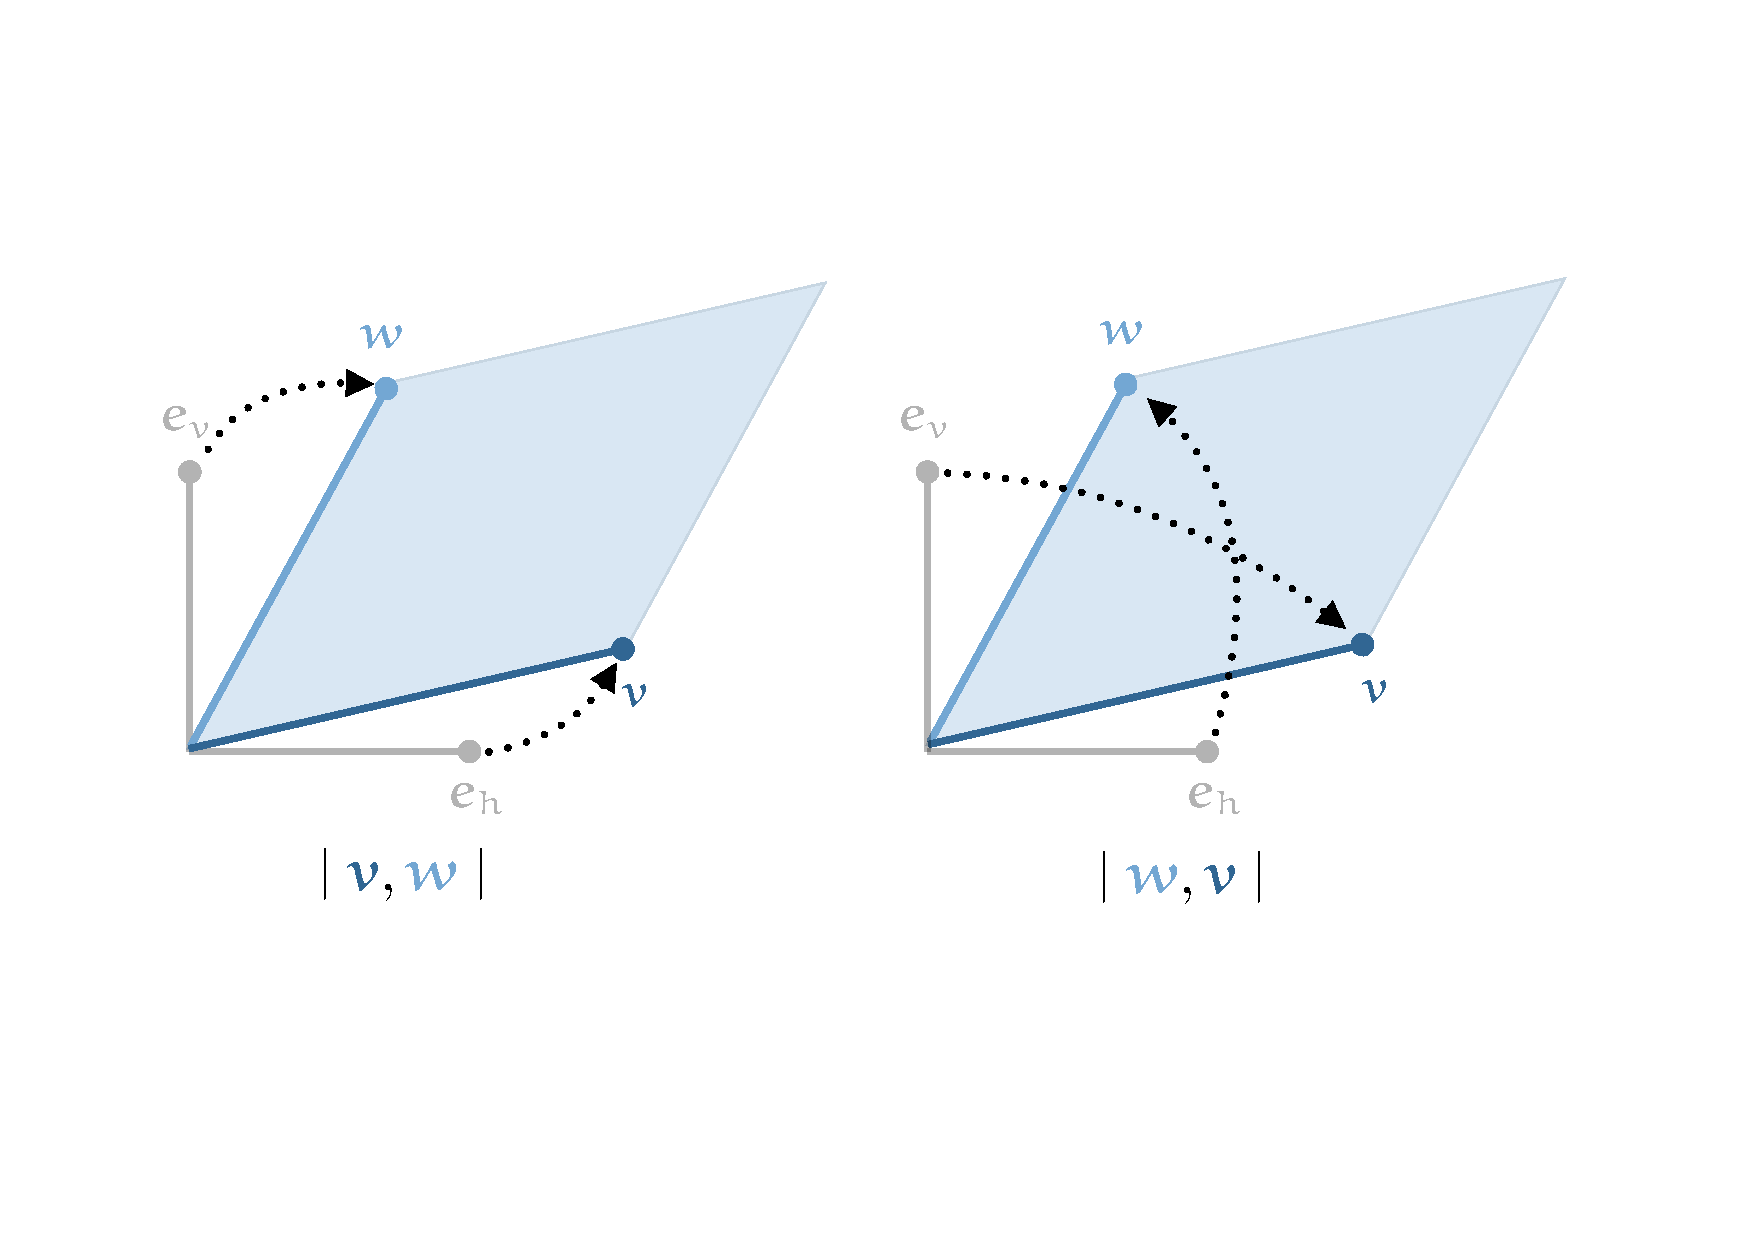
\includegraphics[width=1\textwidth]{./images/pca-3/alternativity.pdf}
	}
	\caption*{Swapping the columns of a matrix swaps the basis vectors of the paralellogram, turning a positive area into a negative area.
	}
\end{figure}

%<figure class="narrow">
%<img src="/images/pca-3/alternativity.svg" />
%<figcaption>Swapping the columns of a matrix swaps the basis vectors of the paralellogram, turning a positive area into a negative area.
%</figcaption>
%</figure>

Put simply, swapping basis vectors around maintains the magnitude of the area of a parallellogram, but changes the signs.

\[
|\;\bc{\mbv}, \lbc{\mbw}\;| = - |\;\lbc{\mbw}, \bc{\mbv}\;| \p
\]

We call this property \textbf{alternativity}. As in, the area of a parallelogram is and alternating function of its basis vectors. 

\index{Alternativity}

With these three properties: skew invariance, multilinearity and alternativity, we can work out our new proof of the determinant formula. First, using multilinearity, we write the first column of matrix \(\bc{\mbA}\) as the sum of two vectors:

\[
\left |\,\begin{matrix} ~a & b \\ c & d\end{matrix}\; \right | = \left | \,\begin{matrix} ~a & b \\ \kc{0} & d\end{matrix}\; \right | + \left | \,\begin{matrix} ~\kc{0} & b \\ c & d\end{matrix}\; \right | \p
\]

We'll call this kind of vector, where only one element is non-zero, a \textbf{simple vector}. Here's a visualization of that step.

\index{Simple vector}\index{Vector!Simple}

\begin{figure}[H]
	\centerline{
		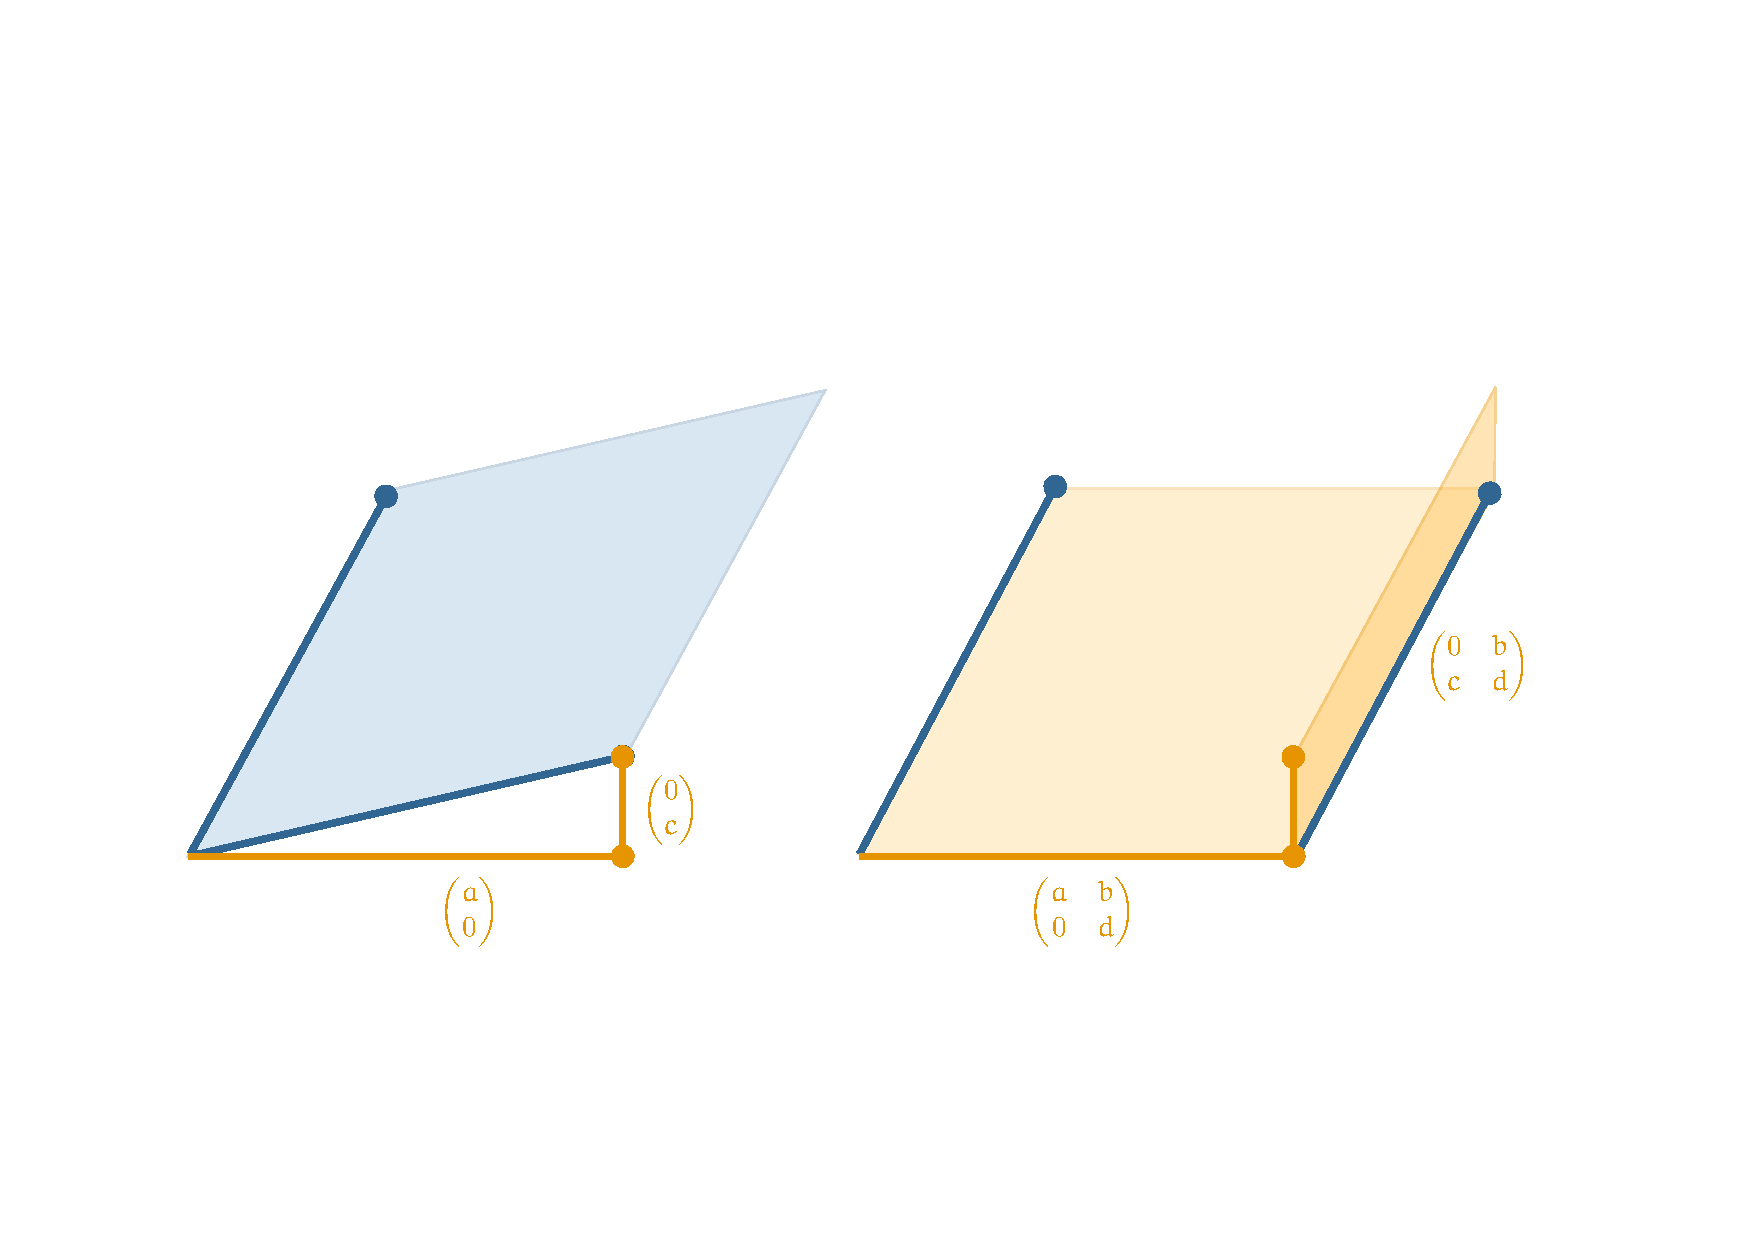
\includegraphics[width=1\textwidth]{./images/pca-3/determinant-step1.pdf}
	}
	\caption*{Breaking the determinant up in to two terms. Note that in the second image, the smaller parallelogram has negative area, because the two basis vectors are reversed.
	}
\end{figure}
%<figure class="narrow">
%<img src="/images/pca-3/determinant-step1.svg" />
%<figcaption>Breaking the determinant up in to two terms. Note that in the second image, the smaller parallelogram has negative area, because the two basis vectors are reversed.
%</figcaption>
%</figure>

Next, we use the property of skew invariance to subtract multiples of these new columns from the others. We use whatever multiple is required to make the rest of the row \(0\). The other rows are unaffected, since these all have \(0\)'s in the original column.

\index{Skew invariance}

\[
\left |\,\begin{matrix} a & b \\ \kc{0} & d\end{matrix}\;\right | + \left |\, \begin{matrix} \kc{0} & b \\ c & d\end{matrix} \;\right | = \left |\, \begin{matrix} a & \kc{0} \\ \kc{0} & d\end{matrix} \right | + \left |\, \begin{matrix} \kc{0} & b \\ c & \kc{0}\end{matrix} \right |\p
\]

Visually, that looks like this.

\begin{figure}[H]
	\centerline{
		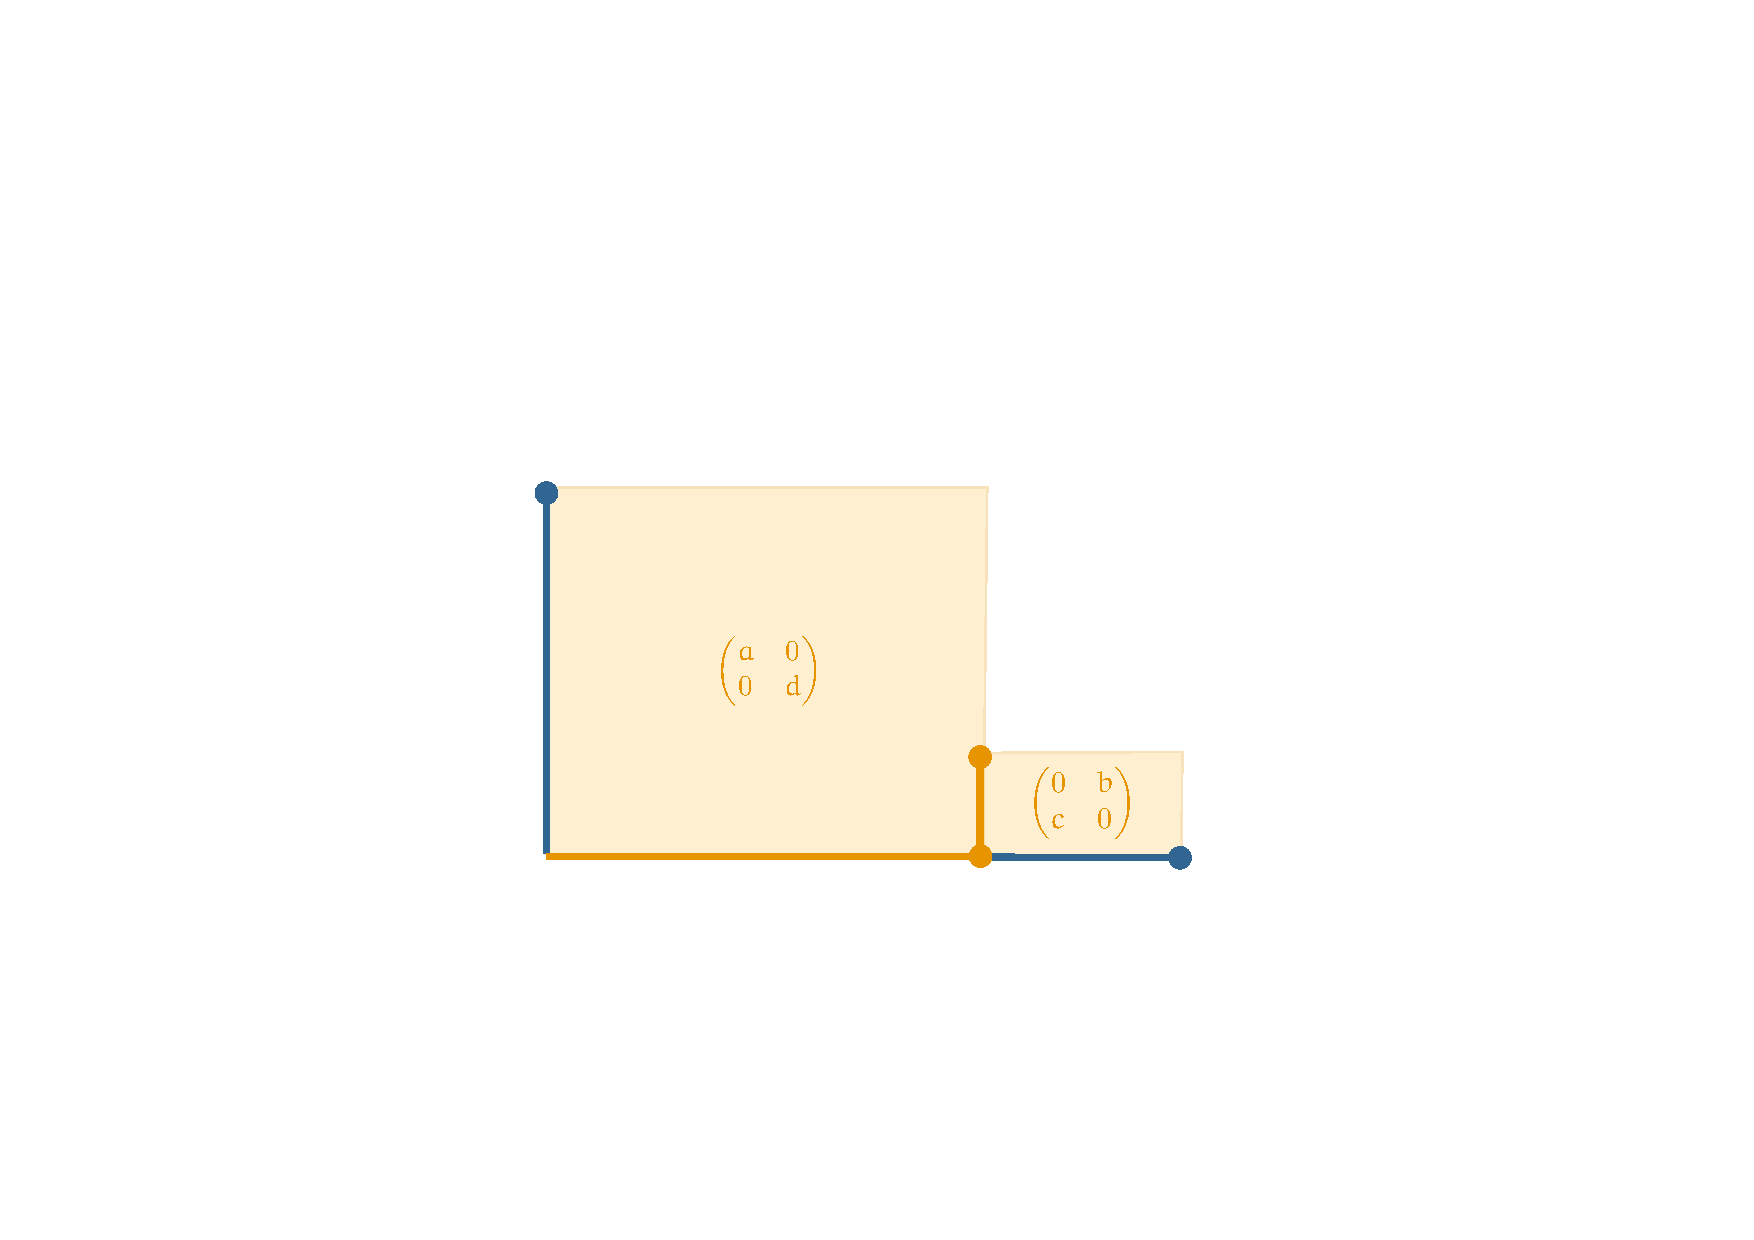
\includegraphics[width=0.8\textwidth]{./images/pca-3/determinant-step2.pdf}
	}
	\caption*{Axis-aligning the remaining basis vectors.
	}
\end{figure}

%<figure class="third center">
%<img src="/images/pca-3/determinant-step2.svg" />
%<figcaption>Axis-aligning the remaining basis vectors.
%</figcaption>
%</figure>

We have two parallelograms with one edge axis-aligned, and we simply skew them so that the other edge is axis-aligned as well. the area we're looking for is now the sum of two rectangles, one of which of facing away from us.

For the first term, we can work out the determinant easily. A diagonal matrix transforms the unit cube to a rectangle, so we just multiply the values along the diagonal: \(ac\). For the second term, we have an anti-diagonal matrix. We can turn this into a diagonal matrix by swapping the two columns. By the property of alternativity, this changes the sign of the area, so the resulting signed area is \(-bc\):

\index{alternativity}


\[
\left |\,\begin{matrix} a & \kc{0} \\ \kc{0} & d\end{matrix} \;\right | + \left |\, \begin{matrix} \kc{0} & b \\ c & \kc{0}\end{matrix} \;\right | \quad=\quad \left |\, \begin{matrix} a & \kc{0} \\ \kc{0} & d\end{matrix} \;\right | - \left |\, \begin{matrix} b & \kc{0} \\ \kc{0} & c\end{matrix} \;\right | \quad=\quad ac - bc \p
\]

This was certainly a more involved way of deriving the formula for the area of a polygon, but the benefit here is that this method generalizes to higher dimensions.

\subsection{Determinants for \(n\times n\) matrices}

We'll start with the three properties we used above, and see how they generalize to higher dimensions. 

\textbf{Skew invariance} also holds in higher dimensions. If we have an \(n \times n\) matrix \(\bc{\mbA}\) with \(n\) column vectors \(\bc{\mba}^1, \ldots, \bc{\mba}^n\), adding a multiple of one to another does not change the volume of the resulting parallelotope. For instance:

\index{Skew invariance}

\[
| \bc{\mbu}, \bc{\mbv}, \bc{\mbw} | = | \bc{\mbu} + \rc{r}\bc{\mbv}, \bc{\mbv}, \bc{\mbw} |
\]

\textbf{Multilinearity} also carries over in the same way. We can break one of the column vectors up into a linear combination of two (or more) other vectors and the area of the resulting paralellotope breaks up in the same way. For instance:
\index{Multilinearity}

\[
| \oc{\mbu}^1 + \oc{\mbu}^2, \bc{\mbv}, \bc{\mbw} | = | \oc{\mbu}^1 , \bc{\mbv}, \bc{\mbw} | + | \oc{\mbu}^2, \bc{\mbv}, \bc{\mbw} |
\]

Finally, \textbf{alternativity}. This requires a little more care. You'd be forgiven for thinking that since we have a higher-dimensional space, we now have more ways for our paralellotope to orient as well. We thought of our paralellogram as a piece of paper which could lie on the table in two ways. If we hold a parallellotope up in space, we can rotate it in all sorts of directions.

\index{Alternativity}

But the metaphor of a piece of paper is slightly misleading. When we flip a piece of paper upside-down, we rotate it, but that's not what really happens when we swap the basis vectors of the paralellogram. What really happens is that we turn the piece of paper inside-out: we \emph{flip} it by pulling the right edge to the left and the left edge to the right.

A better metaphor is a mirror: imagine standing in front of a mirror and holding up your right hand, palm forward.

It looks like your twin inside the mirror is holding up their left hand, with the thumb facing in the opposite direction. But if the mirror flips the image left-to-right, why doesn't it flip the image up-side-down as well? Why doesn't anything change if we turn the mirror ninety degrees?How does the mirror keep track of which direction the floor is?

\begin{figure}[p]
	\centerline{
		\hspace{3.5em}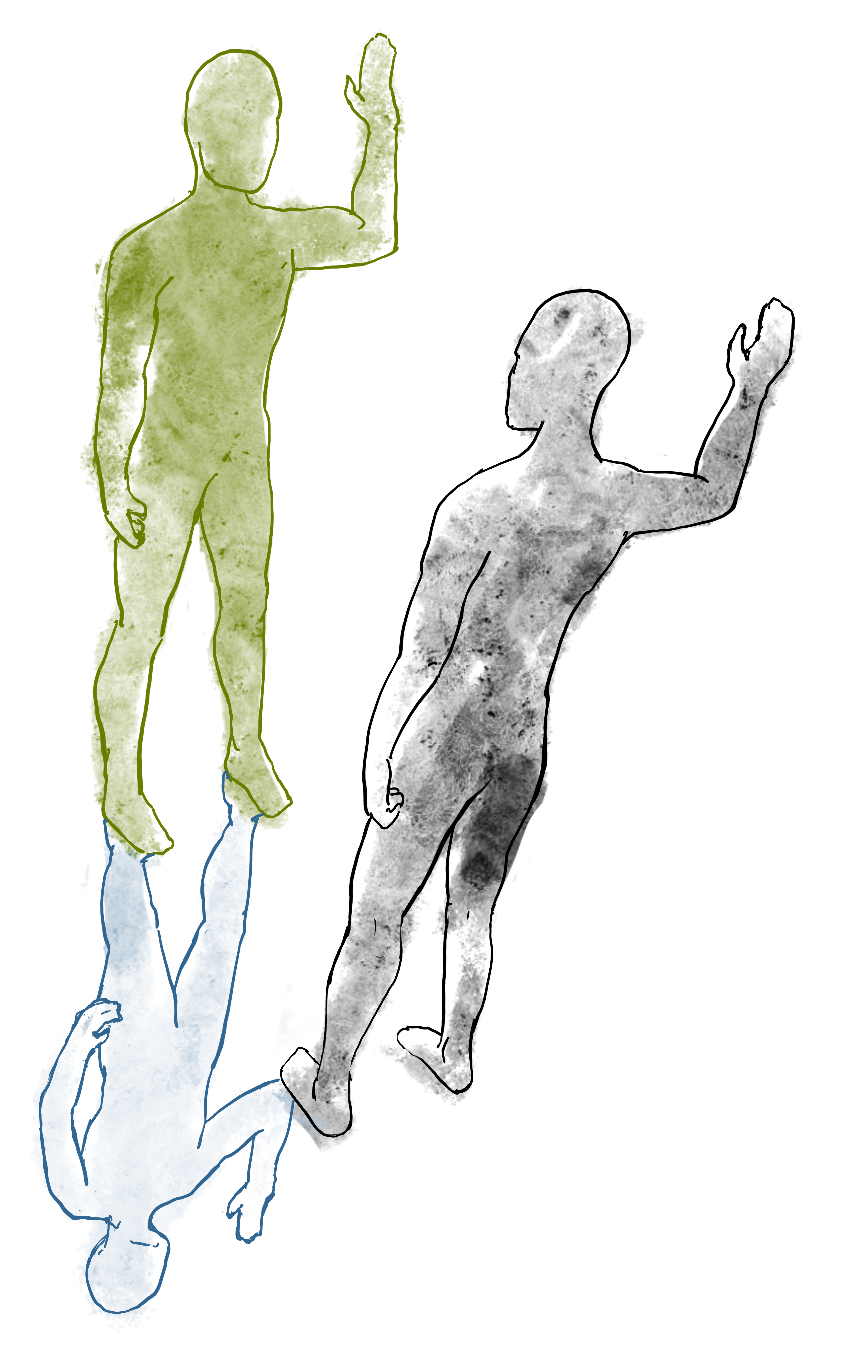
\includegraphics[width=0.8\textwidth]{./images/pca-3/mirrors.png}
	}
	\caption*{A mirror in front of you seems to flip you left-to-right, but it actually flips you \gc{back-to-front}. This \emph{also} turns your right hand into a left hand. A second mirror on the floor flips you \bc{upside-down}, turning your hand back into a right hand again.	}
\end{figure}


The answer is that the mirror \emph{doesn't} flip the image left-to-right. It flips it \emph{back-to-front}. In a manner of speaking, it pulls the back of your hand forward and the front of your hand backwards until the whole hand is flipped. 

\index{Mirror image}

%<figure class="centering">
%<img src="/images/pca-3/mirrors.png" class="three-quarters"/>
%<figcaption>A mirror in front of you seems to flip you left-to-right, but it actually flips you <span class="gc">back-to-front</span>. This also turns your right hand into a left hand. A second mirror on the floor flips you <span class="bc">upside-down</span>, turning your hand back into a right hand again.
%</figcaption>
%</figure>

Putting the mirror to your side will flip you left-to-right, also turning your right hand into a left hand. Putting the mirror on the floor and standing on it turns you upside-down, and again turns the right hand into a left hand. If you use two mirrors, one in front of you and one below, you are flipped back-to-front \emph{and} upside-down, and if you look at this mirror-twin, you'll see that their hand has been flipped twice, to become a right hand again.

The result is that we still have only two orientations. Each time anything gets mirrored, it gets pulled inside out along some line, and the sign of the volume changes: your right hand turns into a left hand and vice versa. If it gets flipped an even number of times the sign stays the same, and if it gets flipped an odd number of times, the sign changes.

This means that alternativity in higher dimensions is defined as follows: if we swap around any two columns in a matrix, we flip the space (along a diagonal between the two corresponding axes). Therefore, the magnitude of the determinant stays the same, but \emph{the sign changes}. If we flip two more axes, the sign changes back. For instance:

\index{Alternativity}

\[
|\; \mbu, \bc{\mbv}, \lbc{\mbw} \;| = - |\; \bc{\mbv}, \mbu, \lbc{\mbw} \;| = |\; \lbc{\mbw}, \mbu, \bc{\mbv} \;| \p
\]

That's our three properties in place. Finally, before we start our derivation, note that in the \(2 \times 2\) case, our ultimate aim was to work the matrix determinant into a sum of determinants of diagonal matrices. The idea was that the determinant of a diagonal matrix is easy to work out.

That's still true in higher dimensions: the columns of a diagonal matrix \(\bc{\mbA}\) each map one of the unit vectors to a a basis vector of length \(\bc{A}_{ii}\) that lies along the \(i\)-th axis. Together these form the sides of an \(n\)-dimensional ``brick'' whose volume is just these lengths multiplied together. So the plan stays the same: use our three properties to rewrite the determinant into a sum of determinants of diagonal matrices.

We'll work this out for a \(3 \times 3\) matrix explicitly as an example, but the principle holds for any number of dimensions.

We start by taking the first column of our matrix, and breaking it up into three simple vectors (using multilinearity).

\index{Simple vector}

\[
\left |\, \begin{matrix} ~a & b & c\\ d & e & f\\ g & h & i \end{matrix}\; \right | = 
\rc{\left |\, \begin{matrix} ~a & b & c\\ \kc{0} & e & f\\ \kc{0} & h & i \end{matrix}\; \right |} +
\gc{\left |\, \begin{matrix} ~\kc{0} & b & c\\ d & e & f\\ \kc{0} & h & i \end{matrix}\; \right |} +
\bc{\left |\, \begin{matrix} ~\kc{0} & b & c\\ \kc{0} & e & f\\ g & h & i \end{matrix}\; \right |}
\]

As before, we've broken our parallellotope into three parallellotopes, each with one of their edges axis-aligned. Next, we subract multiples of the first column from each of the other columns to turn the rows into vectors with only one non-zero element.

\index{Parallellotope}

\[
\rc{\left | \,\begin{matrix} a & \kc{0} & \kc{0}\\ \kc{0} & e & f\\ \kc{0} & h & i \end{matrix} \;\right |} +
\gc{\left | \,\begin{matrix} \kc{0} & b & c\\ d & \kc{0} &  \kc{0}\\ \kc{0} & h & i \end{matrix} \;\right |} +
\bc{\left | \,\begin{matrix} \kc{0} & b & c\\ \kc{0} & e & f\\ g & \kc{0} & \kc{0} \end{matrix} \;\right |}
\]

This doesn't yet look quite as simple as it did in our \(2 \times 2\) case, but we can go back to the first step and break the second column vector of each term into simple vectors as well. For the first term that looks like this:

\[
\rc{\left |\, \begin{matrix} ~a & \kc{0} & \kc{0}\\ \kc{0} & e & f\\ \kc{0} & h & i \end{matrix} \;\right |} = 
\rc{\left |\, \begin{matrix} ~a & \kc{0} & \kc{0}\\ \kc{0} & \kc{0} & f\\ \kc{0} & \kc{0} & i \end{matrix} \;\right |} + 
 \rc{\left |\, \begin{matrix} ~a & \kc{0} & \kc{0}\\ \kc{0} & e & f\\ \kc{0} & \kc{0} & i \end{matrix} \;\right |} +
 \rc{\left |\, \begin{matrix} ~a & \kc{0} & \kc{0}\\ \kc{0} & \kc{0} & f\\ \kc{0} & h & i \end{matrix} \;\right |}
\]

In the first term, one of the column vectors is zero. This means the parallelotope becomes a parallelo\emph{gram}, with \(0\) volume, so we can remove this term. For the other two, we apply the multilinear property to sweep the rows, and we get

\[
\rc{\left |\, \begin{matrix} ~a & \kc{0} & \kc{0}\\ \kc{0} & e & f\\ \kc{0} & h & i \end{matrix} \;\right |} = 
 \rc{\left |\, \begin{matrix} ~a & \kc{0} & \kc{0}\\ \kc{0} & e & \kc{0} \\ \kc{0} & \kc{0} & i \end{matrix} \;\right |} +
 \rc{\left |\, \begin{matrix} ~a & \kc{0} & \kc{0}\\ \kc{0} & \kc{0} & f\\ \kc{0} & h & \kc{0} \end{matrix} \;\right |}
\]

The logic is the same for the \gc{green} and \bc{blue} terms. If we ignore the zeros that we added, we end up with a \(2 \times 2\) submatrix, to which we can apply the same trick again to turn each term into two more terms. If we do this we get six terms in total.

\vspace{0.3em}
\begin{overlong}
 \rc{\left |\, \begin{matrix} a & \kc{0} & \kc{0}\\ \kc{0} & e & \kc{0} \\ \kc{0} & \kc{0} & i \end{matrix}\; \right |} +
 \rc{\left | \,\begin{matrix} a & \kc{0} & \kc{0}\\ \kc{0} & \kc{0} & f\\ \kc{0} & h & \kc{0} \end{matrix} \;\right |} +
 \gc{\left | \,\begin{matrix} \kc{0} & b & \kc{0} \\ d & \kc{0} &  \kc{0}\\ \kc{0} & \kc{0} & i \end{matrix} \;\right |} +
 \gc{\left | \,\begin{matrix} \kc{0} & \kc{0} & c\\ d & \kc{0} &  \kc{0}\\ \kc{0} & h & \kc{0} \end{matrix}\; \right |} +
 \bc{\left |\, \begin{matrix} \kc{0} & b & \kc{0}\\ \kc{0} & \kc{0} & f\\ g & \kc{0} & \kc{0} \end{matrix}\; \right |} + 
\bc{\left | \,\begin{matrix} \kc{0} & \kc{0} & c\\ \kc{0} & e & \kc{0}\\ g & \kc{0} & \kc{0} \end{matrix}\; \right |}
\end{overlong}
\vspace{0.7em}

\noindent The result is that we have separated the determinant into several terms, so that for each, the matrix in that term has only one non-zero element in each row and each column. The structure of the non-zero values is that of a \emph{permutation matrix}, with the exception that permutation matrices contain only \(1\)s and \(0\)s. These are like the original matrix \(
\bc{\mbA}\) with a permutation matrix used to mask out certain values.

\index{Permutation matrix}

In fact, what we have done is to enumerate \emph{all possible permutations}. We started by creating one term for each possible choice for the first column, and then for each term we separated this in to the remaining two choices for the second column (after which the choice for the third column was fixed as well).

\index{Permutation}

This idea naturally generalizes to higher dimensions. Moving from left to right, we pick one element of each column and zero out the rest of its column and row. At each subsequent step we limit ourselves to whatever non-zero elements remain. We sum the determinants of all possible ways of doing this.

\noindent We can now turn each of these matrices into a diagonal matrix, by swapping around a number of columns. By the property of alternativity, this doesn't change the magnitude of the determinant, only the sign: for an even number of swaps, it stays the same and for an odd number it flips around. This gives us 

\vspace{0.3em}
\begin{overlong} \rc{\left| \,\begin{matrix} a & \kc{0} & \kc{0}\\ \kc{0} & e & \kc{0} \\ \kc{0} & \kc{0} & i \end{matrix}\; \right |} -
 \rc{\left | \,\begin{matrix} a & \kc{0} & \kc{0}\\ \kc{0} & f & \kc{0} \\ \kc{0} & \kc{0} & h\end{matrix}\; \right |} -
 \gc{\left |\, \begin{matrix} b & \kc{0} & \kc{0} \\ \kc{0} & d & \kc{0}\\ \kc{0} & \kc{0} & i \end{matrix}\; \right |} +
 \gc{\left | \,\begin{matrix} c & \kc{0} & \kc{0} \\  \kc{0} & d &  \kc{0}\\ \kc{0} & \kc{0} & h \end{matrix}\; \right |} +
 \bc{\left |\, \begin{matrix} b & \kc{0}  & \kc{0}\\ \kc{0} & f & \kc{0} \\ \kc{0} & \kc{0} & g \end{matrix} \;\right |} - 
\bc{\left |\, \begin{matrix} c & \kc{0} & \kc{0} \\ \kc{0} & e & \kc{0}\\ \kc{0} & \kc{0} & g\end{matrix} \;\right |} 
\p
\end{overlong}
\vspace{0.7em}

\noindent And since the determinant of a diagonal matrix is simply the diagonal product, as we worked out earlier, we get

\[
\left |\,\begin{matrix} a & b & c\\ d & e & f\\ g & h & i \end{matrix} \; \right | =
\rc{aei} - \rc{afh} - \gc{bdi} + \gc{cdh} + \bc{bfg} + \bc{ceg} \p
\]

To generalize this to \(n\) dimensions, we represent a permutation of the first \(n\) natural numbers with the symbol \(\sigma\). For instance, if \(n=6\) we may have \(\sigma = \langle 1, 5, 4, 3, 2\rangle\). We'll call the \emph{sign} of a permutation, \(\text{sign}(\sigma)\), \(-1\) if the permutation can be placed in the correct order with an odd number of swaps and \(1\) if this can be done with an even number of swaps.

%Then, for a given \(n \times n\) matrix \(\bc{\mbA}\), let \(\bc{\mbA}^\sigma\) be the matrix constructed by taking \(\bc{\mbA}\) and zeroing out any element that doesn't have an index of the form \((\sigma_i, i)\). That is, iterate over the columns \(i\), mark the element in that column at row \(\sigma_i\), and zero out the rest.

 
Then, the process we described above leads to the following formula for the determinant:

\[
|\bc{\mbA}| = \sum_\sigma \text{sign}(\sigma) \prod_i \bc{A}_{\sigma(i), i}
\]

where the sum is over all permutations of the first \(n\) natural numbers, and the product runs from \(1\) to \(n\).

Note that for each term in our sum, corresponding to the permutation \(\sigma\), the value \(\bc{A}_{\sigma(i), i}\) marks out one of the elements that we haven't zeroed out. The value \(\prod_i \bc{A}_{\sigma(i), i}\) is the product of all these values.


This is called the \textbf{Leibniz formulation} of the determinant. 

\index{Leibniz formulation}\index{Determinant!Leibniz formulation}

\begin{aside}We got here by defining the determinant as the volume of a parallelotope and then deriving the Leibniz formulation from that. This is useful for building a visual intuition, but if you want to be rigorous it's not the most efficient approach.

For this reason, the determinant is usually first defined as \emph{any} multilinear, alternative function, which yields 1 for the identity matrix. You can then show that there is only one such function, and that it's the Leibniz function above. From there, you can then prove all the other interpretations of the determinant, including the geometrical one.
\end{aside}

%<!-- 
%
%### Computing determinants for \(n\times n\) matrices: Laplace expansion
%
%How do we scale this up to higher dimensions? For \(n\times n\) matrices, computing the determinant is not quite as simple as subracting one diagonal product from another. Geometrically, the principle is the same: in three dimensions, we transform the unit cube into a parallelepiped (a 3D parallelogram) and work out its volume. In \(n\) dimensions we transform a hypercube into the n-dimensional equivalent of a paralellogram, called a _parallelotope, and work out its hypervolume. The drawback here is that the formulae for these (hyper)volumes are not straightforward.
%
%Here's some intuition to help us along. The sides of a parallelepiped are parallellograms. The sides of a 4D parallelotope are paralellepipeds, and so on. Can we somehow build up from what we know, using the formula for area to compute the volume and then use the formula for volume to compute the 4D volume and so on?
%
%This is the basis behind the _Laplace expansion_. We take the \(n \times n\) matrix for whcih we want to compute the determinant, slice out a number of matrices of one "dimension" lower (\(n-1 \times n-1\) matrices), compute _their_ determinants, and then work out the determinant of the original matrix as a function of these.
%
%The Laplace expansion is a recursive algorithm: given an \(n \times n\) matrix, we slice out a series of \((n-1) \times (n-1)\) matrices, compute _their_ determinants, and then combine them to compute the determinant of the  \(n \times n\) matrix. How do we compute the determinants of the smaller matrices? We uses their Laplace expansions (slicing out \((n-2) \times (n-2) matrices)\) and so on, until the slices are \(2 \times 2\) and we can use the simple function we discovered above.
%
%<p>Here's how it works in detail. Given an \(n \times n\) matrix \(\bc{\A}\), let \(\bc{\A}^{ij}\) be the result of removing the \(i\)-th row and \(j\)-th column of \(\bc{\A}\). This is called a <em>minor</em> of \(\bc{\A}\). Since we've removed one row and one column, each minor is an \((n-1) \times (n-1)\) matrix.</p>
%
%<aside>Note the boldface: \(\bc{\A}^{ij}\) is a matrix, whereas \(\bc{A}_{ij}\) is a scalar (one element of \(\bc{\A}\)).
%</aside>
%
%Fixing row \(i=\rc{1}\) and iterating over the columns \(\gc{j}\), we can now compute the determinant as
%
%\[
%\text{det}\;\bc{\A} = \bc{A}_{\rc{1}\gc{1}}\text{det}\bc{\A}^{\rc{1}\gc{1}} - \bc{A}_{\rc{1}\gc{2}}\text{det}\; \bc{\A}^{\rc{1}\gc{2}} + \bc{A}_{\rc{1}\gc{3}}\text{det}\; \bc{\A}^{\rc{1}\gc{3}} + \ldots \pm \bc{A}_{\rc{1}\gc{n}}\text{det}\;\bc{\A}^{\rc{1}\gc{n}} \p
%\]
%
%Note that the sign of the terms alternates, so the last term is positive or negative depending on whether \(n\) is odd or even.
%
%<aside> The choice of row is arbitrary. It works with any other row \(i\) too, so long as the term for each minor \(\bc{\A}^{ij}\) is positive if \(i+j\) is even and negative if it is odd.
%</aside>
%
%We can apply this method recursively until the matrices are \(2 \times 2\), and then work backwards from there. 
%
%It's not very intuitive why this method should work to give us the determinant. Laplace himself most likely worked this out by taking _Cramer's rule_, an equality containing the minors of a matrix and the determinant, and rewriting the terms. For our purposes, that adds even more baggage, and it takes us away from the neat geometric interpretation of the \(2 \times 2\) case. 
%
%Can we work out a similarly geometric interpretation for the Laplace's formula? It turns out that you can, with relative ease, using something called _Geometric algebra_. This is a bit of a diversion, so I've moved it to the appendix. If you're happy to take Laplace at his word, then read on, but if you have the time, geometric algebra is an extremely useful generalization in geometry.
% -->
%
%<!-- The determinant is a very useful tool, but we need it only for one purpose: to tell us which matrices are invertible. The reason we need this is because it allows us to relate the eigenvalues of a matrix to the roots of a particular polynomial defined from a matrix, called the characteristic polynomial. -->


The determinant is a powerful tool, with many uses. Here, we only care about one of them: \emph{it lets us characterize whether a matrix is invertible or not}. The determinant is precisely zero if and only if the matrix is not invertible. The reason we care about this, is that it will lead to a very useful way of characterizing the eigenvalues: the \textbf{characteristic polynomial} of a matrix.

\section{The characteristic polynomial}
\index{Characteristic polynomial}

Let's start with how we originally characterized eigenvalues in Chapter~\ref{chapter:eigenvectors}. There, we said that an eigenvector of a matrix \(\bc{\mbA}\) is any vector \(\rc{\mbv}\) for which the direction doesn't change, under operation of the matrix. The magnitude \emph{can} change, and the increase of that magnitude we call the eigen\emph{value} \(\bc{\lambda}\) corresponding to the eigenvector.

To summarize, for any eigenvector \(\rc \mbv\) and its eigenvalue \(\bc{\lambda}\) of \(\bc \mbA\), we have

\[
\bc{\mbA}\rc{\mbv} = \bc{\lambda}\rc{\rc{\mbv}} \p
\]

Moving the right-hand-side over to the left, we get 

\[
\bc{\mbA}\rc{\mbv} - \bc{\lambda} \rc{\mbv} = {\mathbf 0} \text{,}
\]

where both sides are vectors, with a vector of zeros on the right. To allow us to manipulate the left hand side further we rewrite \(\bc{\lambda}\rc{\mbv}\) as \((\bc{\lambda}\mbI)\rc{\mbv}\). This gives us:

\begin{align*}
\bc{\mbA}\rc{\mbv} - \bc{\lambda}\mbI\rc{\mbv} &= {\mathbf 0}  \\
(\bc{\mbA} - \bc{\lambda}\mbI)\rc{\mbv} &= {\mathbf 0} \p 
\end{align*}

This last line is basically a linear problem of the form \(\bc{\mbM}\rc{\mbv} = \mathbf 0\), with \(\bc{\mbM} = (\bc{\mbA} - \bc{\lambda}\mbI)\). The solutions to this problem, the set of all vectors \(\rc \mbv\) that we can multiply by \(\bc{\mbM}\) to get the null vector \(\mathbf 0\) are called the \emph{null space} of \(\bc{\mbM}\). What we have just shown is that \textbf{any eigenvector of \(\bc \mbA\) with eigenvalue \(\bc \lambda\) must be in the null space of the matrix \(\bc{\mbA} - \bc{\lambda}\mbI\)}.

This is where invertibility and the determinant come in: if \(\bc \mbM\) is invertible, it can only map one point to any other point. Every matrix maps \(\mathbf 0\) to \(\mathbf 0\), so for any invertible matrix the null space consists only of the point \(\mathbf 0\). The only matrices with more interesting null spaces are non-invertible matrices. Or, matrices with determinant \(0\). 

\begin{aside}%
Note that we're not talking about the invertibility of \(\bc \mbA\) itself, only of the derived matrix \(\bc{\mbM} = \bc{\mbA} - \bc{\lambda}\mbI\)
\end{aside}

So, now we can tie it all together. Choose some scalar value \(\bc \lambda\). If we have 

\[\left | \; \bc{\mbA} - \bc{\lambda}\mbI \;\right | = 0\]

then the matrix \(\bc{\mbA} - \bc{\lambda}\mbI\) has a non-trivial null-space, and \(\bc \lambda\) is an eigenvalue. We want to study the left-hand-side of this equation as a function of \(\bc{\lambda}\), taking the values in \(\bc{\mbA}\) as constants.

As we've seen, expanding the determinant into an explicit form can get a little hairy for dimensions larger than 3, but we don't need to make it explicit, so long as we can tell what \emph{kind} of function it is. To illustrate, say we have a \(2 \times 2\) matrix 

\[
\bc \mbA = \begin{pmatrix}a & b \\ c & d\end{pmatrix} \p
\]

In that case, the value \(\left |\,\bc{\mbA} - \bc{\lambda}\mbI\,\right|\) works out as

\[
(a-\bc{\lambda})(d - \bc{\lambda}) - bc \p
\]

We can multiply out these brackets, and we would see that this is a polynomial with \(\bc{\lambda}\) as its variable. This polynomial has \(\bc{\lambda}^2\) as the highest power. The values for which this polynomial equal zero, its \textbf{roots}, are the eigenvalues of the original matrix \(\bc{\mbA}\).

\noindent For an \(n\times n\) matrix, as we saw, the Leibniz form of the determinant gives us one term for each possible permutations of length \(n\), each of which consists of \(n\) elements of the matrix multiplied together. If any of these elements come from the diagonal, they contain \(\bc{\lambda}\). That means each term contains at most \(n\) \(\bc{\lambda}\)s, giving us an \(n\)-th order polynomial.

As you may have guessed, this function is what we call the \textbf{characteristic polynomial} of \(\bc{\mbA}\). The points where this function is \(0\), the roots of the polynomial, are the eigenvalues of \(\bc{\mbA}\). 

And this means that we can apply a whole new set of tools from the analysis of polynomials, to the study of eigenvectors. We never have to work out the characteristic polynomial explicitly, we can just use the knowledge that the determinant \emph{is a polynomial} and use what we know about polynomials to help us further along towards the spectral theorem.

And one of the richest and most versatile tools to come out of the analysis of polynomials, is the idea of \emph{complex numbers}. This is a counterintuitive idea, so we'll take some time to set it up carefully, before we dig into the mathematics.

\section{Complex numbers}
\index{Complex numbers}

Complex numbers spring from the idea that there exists a number \(i\) for which \(i^2\) is \(-1\). We don't know of any such number, but we simply assume that it exists, and investigate the consequences. For many people this is the point where mathematics becomes too abstract and they tune out. The idea that squares can be negative clashes too much with our intuition for what squares are. The idea that we just pretend that they can be negative and keep going, seems almost perverse.

And yet, this approach is one that humanity has followed again and again in the study of numbers. If you step back a bit, you start to see that it is actually one of the most logical and uncontroversial things to do. 

The study of numbers started somewhere before recorded history, in or before the late stone age, when early humans began counting things in earnest, and they learned to \emph{add}. I have five apples, I steal three apples from you, now I have eight apples. That sort of thing.

\noindent At some point, these early humans will have solidified their concept of ``numbers.'' It is a set of concepts (whose meaning we understand intuitively) which starts \(1, 2, 3, \ldots\) and continues. If you add one number to another, you always get another number.  If the number was big, they may not have had a name for it, but a patient paleolithic human with enough time could certainly have carved the required number of tally marks into an animal bone.

The operation of addition can also be reversed. If \(5 + 3\) gives \(8\), then taking \(5\) away from \(8\) gives \(3\). If I steal \(5\) apples from your collection of \(8\), you still have \(3\) left. Thus, subtraction was born. But subtraction, the \emph{inverse} of addition, required some care. Where adding two numbers always yields a new number, subtracting two numbers doesn't always yield a new number. You can't have \(5 - 8\) apples, because if you have \(5\) apples I can't steal more than \(5\) of them.

As societies grew more complicated, financial systems developed and \emph{debt} became an integral part of daily life. At some point, the following thought experiment was considered. What if \(5-8\) is a number after all? Maybe it's just a number we don't have a name for yet.

So, we'll just give it a name and see if we can make some sense of how it behaves. No doubt many people were outraged by such a suggestion, protesting that it was unnatural, and an insult to whatever God they believed had designed the numbers. But simple investigation soon showed that if these numbers were assumed to exist, they followed simple rules and, it made sense to think of them as a kind of mirror image of the natural numbers, extending to infinity in the opposite direction. \(5 - 8\) was the mirror image of \(3\), so it made sense to call it ``\(-3\)''.

\index{Negarive numbers}

The skeptics might argue that this made no sense, because there is no such thing as having \(-3\) apples, but the mathematicians will have countered that in other areas, such as finance, there were concepts that could be expressed very beautifully by the negative numbers. If I owe you \(3\) apples, because my earlier theft was found out, but you also stole \(8\) apples from me, I now owe you \(-5\) apples, or rather, you owe me \(5\).

The same principle can be applied to multiplication. If your tribe has \(8\) families, and every family is entitled to \(5\) apples, you need to find \(8 \times 5\) apples. Again, an operator, and any two numbers you care to multiply will give you a new number (even if you believe in negative numbers).

And again, you can do the reverse the operation: if the harvest has yielded \(48\) apples, you can work out that every family in your tribe gets \(6\) of them. But again, you have to be careful about which numbers you apply the inverse to. Sometimes you get a known number, and sometimes you don't. If you have 50 apples, suddenly there is no known number that is the result of \(50/8\).

But what if there was? What if we just gave \(50/8\) a name and started investigating? We'd find out pretty quickly that it would make sense to think of these numbers as lying \emph{in between} the integers. We call these the \emph{rational} numbers. Whoever it was that invented the rationals must have run into less resistance than the inventor of the negative numbers; it's much easier to imagine half an apple than to imagine \(-3\) of them.

The pattern is hopefully becoming clear. Let's have one more example, to really drive the point home, and also to bring us far enough into recorded history so we can actually see how people dealt with these revelations. Adding is repeated counting, and multiplication is repeated adding so \emph{raising to a power}, repeated multiplication, is the next operator in the hierarchy. 

The story should be familiar at this point. Any two natural numbers \(a\) and \(b\) can be "exponentiated" together as \(a^b\) and the result is another natural number.

\index{Exponentiation}

The inverse operation is a b-th root, but we can stick with square roots to illustrate our point. In fact the square root of 2, the length of the diagonal of a unit square, is all we need. In this case, there is nothing abstract or perverse about the quantity \(\sqrt 2\): in a square room with sides of 1 meter it's the distance from one corner to the corner opposite.
\enlargethispage{4em}

\begin{figure}[H]
	\centerline{
		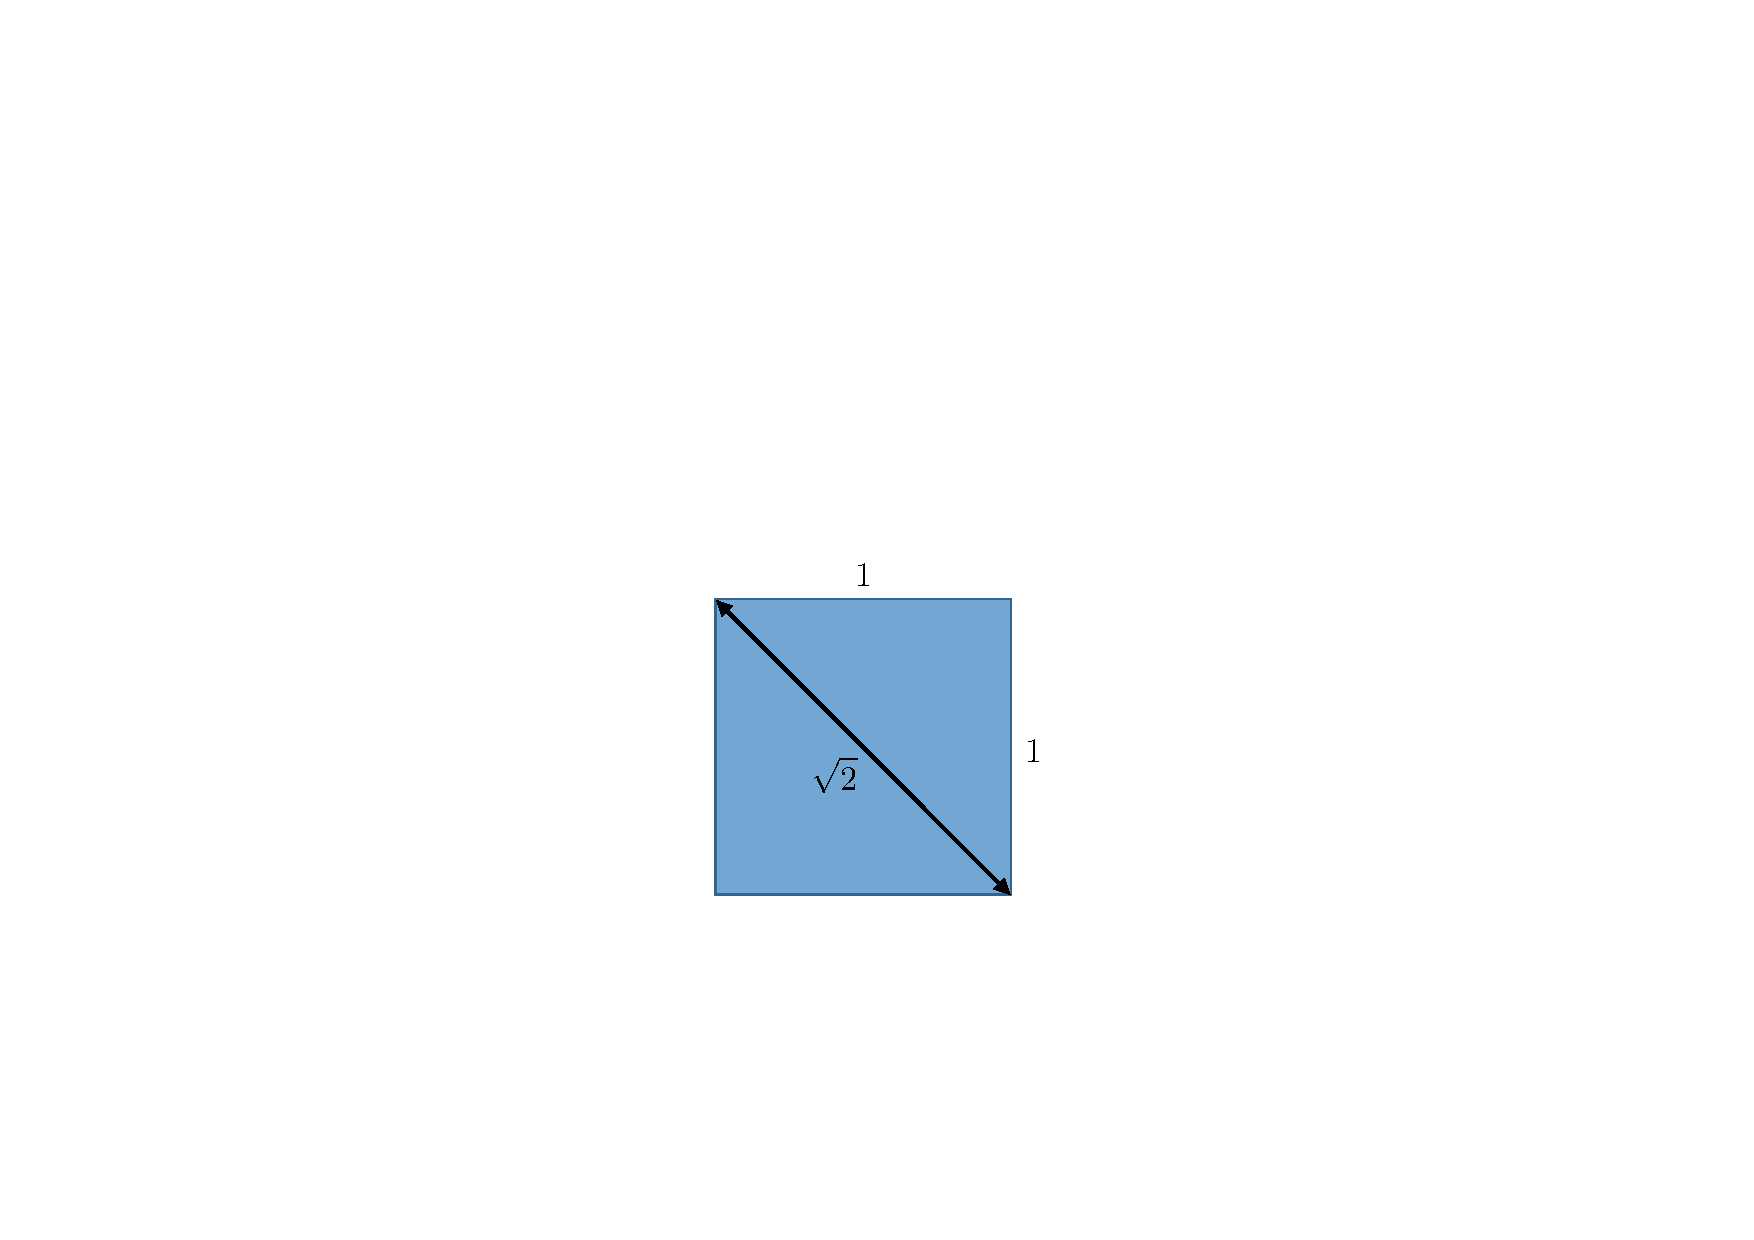
\includegraphics[width=0.4\textwidth]{./images/pca-3/sqrt2.pdf}
	}
\end{figure}

%<figure class="centering">
%<img src="/images/pca-3/sqrt2.svg" class="tile4"/>
%<figcaption>
%</figcaption>
%</figure>

And yet, when people investigated, it caused great upset.

The man who gave his name to the theorem we would use to work out the above picture, Pythagoras, was the head of a cult. A cult dedicated to mathematics. They lived ascetically, much like monks would, centuries later, and dedicated themselves to the study of nature in terms of mathematics. When asked what the purpose of man was, Pythagoras answered ``to observe the heavens.'' One fervent belief of the Pythagoreans was that number and geometry were inseparable: all geometric quantities could be expressed by (known) numbers.

\index{Pythagoras}\index{Pythagoreans}

The story of the Pythagoreans is a mathematical tragedy. It was one of their own, commonly identified as Hippasus of Metapontum, who showed that no rational number corresponded exactly to \(\sqrt{2}\). Some aspects of geometry were outside the reach of the known numbers. According to legend, he was out at sea when he discovered this, and was promptly thrown overboard by the other Pythagoreans.

\index{Hippasus of Metapontum}

Of course, with the benefit of hindsight, we know how to manage such upsetting discoveries. We simply give the new number a name, ``\(\sqrt{2}\),'' and see if there's some place among the numbers where it makes sense to put it. In this case, somewhere between \(141/100\) and \(142/100\), in a space we can make infinitely small by choosing better and better rational approximations.

With this historical pattern clearly highlighted, the discovery of the complex numbers should be almost obvious. In fact, we don't even need a new operation to invert, we are still looking at square roots, but instead of applying the square root a positive integer, we apply it to a \emph{negative integer}. To take the simplest example, we'll look at  \(\sqrt{-1}\). No number we know gives \(-1\) when we multiply it by itself, so our first instinct is to dismiss the operation. The square root is only allowed for a subset of the real-valued numbers. Just like subtraction was only allowed for a subset of the natural numbers, and division was only allowed for a subset of the integers.

But, what if the number \(\sqrt{-1}\) did exist? What would the consequences be?

As the previous paragraphs should illustrate, this kind of investigation is usually born out of necessity. Like a fussy child given a new food, people are consistently reluctant to accept new types of numbers. In this case, what pushed us over the edge was the study of polynomials; functions of the form: 

\[f(x) = \bc{a}x^3 + \bc{b}x^2 + \bc{c}x + \bc{d}\] 

where the highest exponent in the sum indicates the \emph{order} of the polynomial.

The problem of finding the \emph{roots} of a polynomial, the values of \(x\) for which \(f(x)\) is equal to \(0\) crops up in all sorts of practical problems. In some cases, this leads to squares of negative numbers, as we see when we try to solve \(\gc{x^2 + 1 = 0}\). This didn't worry anybody, of course, since this function lies entirely above the horizontal axis---it has no roots---so it's only natural that solving for the roots leads to a contradiction. 

\index{Roots of a polynomial}\index{Polynomial!roots of}

\begin{figure}[H]
	\centerline{
		\includesvg[width=0.8\textwidth]{./images/pca-3/polynomials.svg}
	}
	\caption*{The function \(f(x) = x^2 + 1\) has no roots: it doesn't cross the horizontal axis. Therefore, it make sense that \(x^2 = 0\) or \(\sqrt{-1}\) has no solutions.	}
\end{figure}

%<figure class="half center">
%<img src="/images/pca-3/polynomials.svg">
%<figcaption>The function \(f(x) = x^2 + 1\) has no roots. This makes total sense, since it doesn't cross the horizontal axis.
%</figcaption>
%</figure>

However, when people started to work out general methods for finding the roots of \emph{third}-order polynomials, like \(\bc{x^3 - 15x - 4}\), which \emph{does} have roots, it was found that the methods worked if one temporarily accepted \(\sqrt{-1}\) as an intermediate value, which later canceled out. This is where the phrase \emph{imaginary} number originates. People (Descartes, to be precise) were not ready to accept these as numbers, but no one could deny their utility.

\index{Descartes}

Eventually, people followed the pattern that they had followed for the integers, the rationals and all their successors. We give the new number a name, \(i = \sqrt{-1}\), and we see if there's any way to relate it, geometrically, to the numbers we know.

Let's start with addition. What happens if we add \(i\) to some number, say \(3\)? The simple answer is that nothing much happens. The most we can say about the new number is that it is \(3 + i\). 

\index{Complex numbers!addition}

Multiplication then. Again \(2 \times i\) doesn't simplify in any meaningful way, so we'll just call the new number \(2i\). What if we combine the two? With a few subtleties, we can rely on the basic rules of algebra to let us multiply out brackets and add things together. So, if we start with \(i\), add 3 and multiply by 2, we get:

\index{Complex numbers!multiplication}

\begin{align*}
2(i + 3) = 2\cdot3 + 2\cdot i = \bc{6} + \rc{2}i 
\end{align*}

This is a very common result: we've applied a bunch of operations, involving the imaginary number \(i\), and the result can be written as the combination of a real value \(\bc{r}\), another real value \(\rc{c}\) and \(i\) as:

\[
\bc{r} + \rc{c}i \p
\]

\index{Complex numbers!Cartesian notation}

We will call any number that can be written in this way a \emph{complex number}. The set of all complex numbers is written as 

\[{\Large \mathbb C} \p\]

\index{\(\mathbb C\)}

At this point you may be worried. What if we come up with another operation that is not defined for all complex numbers? Are we going to have to make another jump? Are we going to find ever bigger families of numbers to deal with? It turns out that in many ways, \(\mathbb C\) is the end of the line. So long as we stick to algebraic operations, we can do whatever we like to complex numbers, and the result will always be well defined as another complex number.

\pagebreak 

% !!!
%\setlength\parfillskip{0pt plus .6\textwidth}
%\setlength\emergencystretch{2pt}

\noindent To illustrate, let's show this for a few simple examples. Lets say we have two complex numbers \(\gc{a} + \gc{b}i\) and \(\oc{c} + \oc{d}i\). If we add them, we get

\[(\gc{a} + \gc{b}i) + (\oc{c} + \oc{d}i) = \gc{a} + \oc{c} + \gc{b}i + \oc{d}i = \bc{(a + c)} + \rc{(b + d)}i
\]

\index{Complex numbers!addition}

If we multiply them, we get

\begin{align*}
(\gc{a} + \gc{b}i)(\oc{c} + \oc{d}i) &= \gc{a}\oc{c} + \gc{a}\oc{d}i + \gc{b}i\oc{c} + \gc{b}i\oc{d}i \\
&= (\gc{a}\oc{d} + \gc{b}\oc{d}\kc{i^2}) + (\gc{a}\oc{d} + \gc{b}\oc{c})i \\
&= \bc{ad - bd} + \rc{(ad + bc)}i \p
\end{align*}

That is, one \bc{real-valued number}, added to \(i\) times another \rc{real-valued number}. Note that in the second line of the derivation for the multiplication, we can use \(\kc{i^2} = -1\), since we know that \(i = \sqrt{-1}\). In short, multiplying or adding together any two complex numbers gives us another complex number. 

\index{Complex numbers!multiplication}

Since every complex number can be written as the combination of two real-valued numbers, it makes sense to visualize them in a plane. We plot the value of the \bc{real term} along the horizontal axis and the value of the \rc{imaginary term} along the vertical. 

\begin{figure}[H]
	\centerline{
		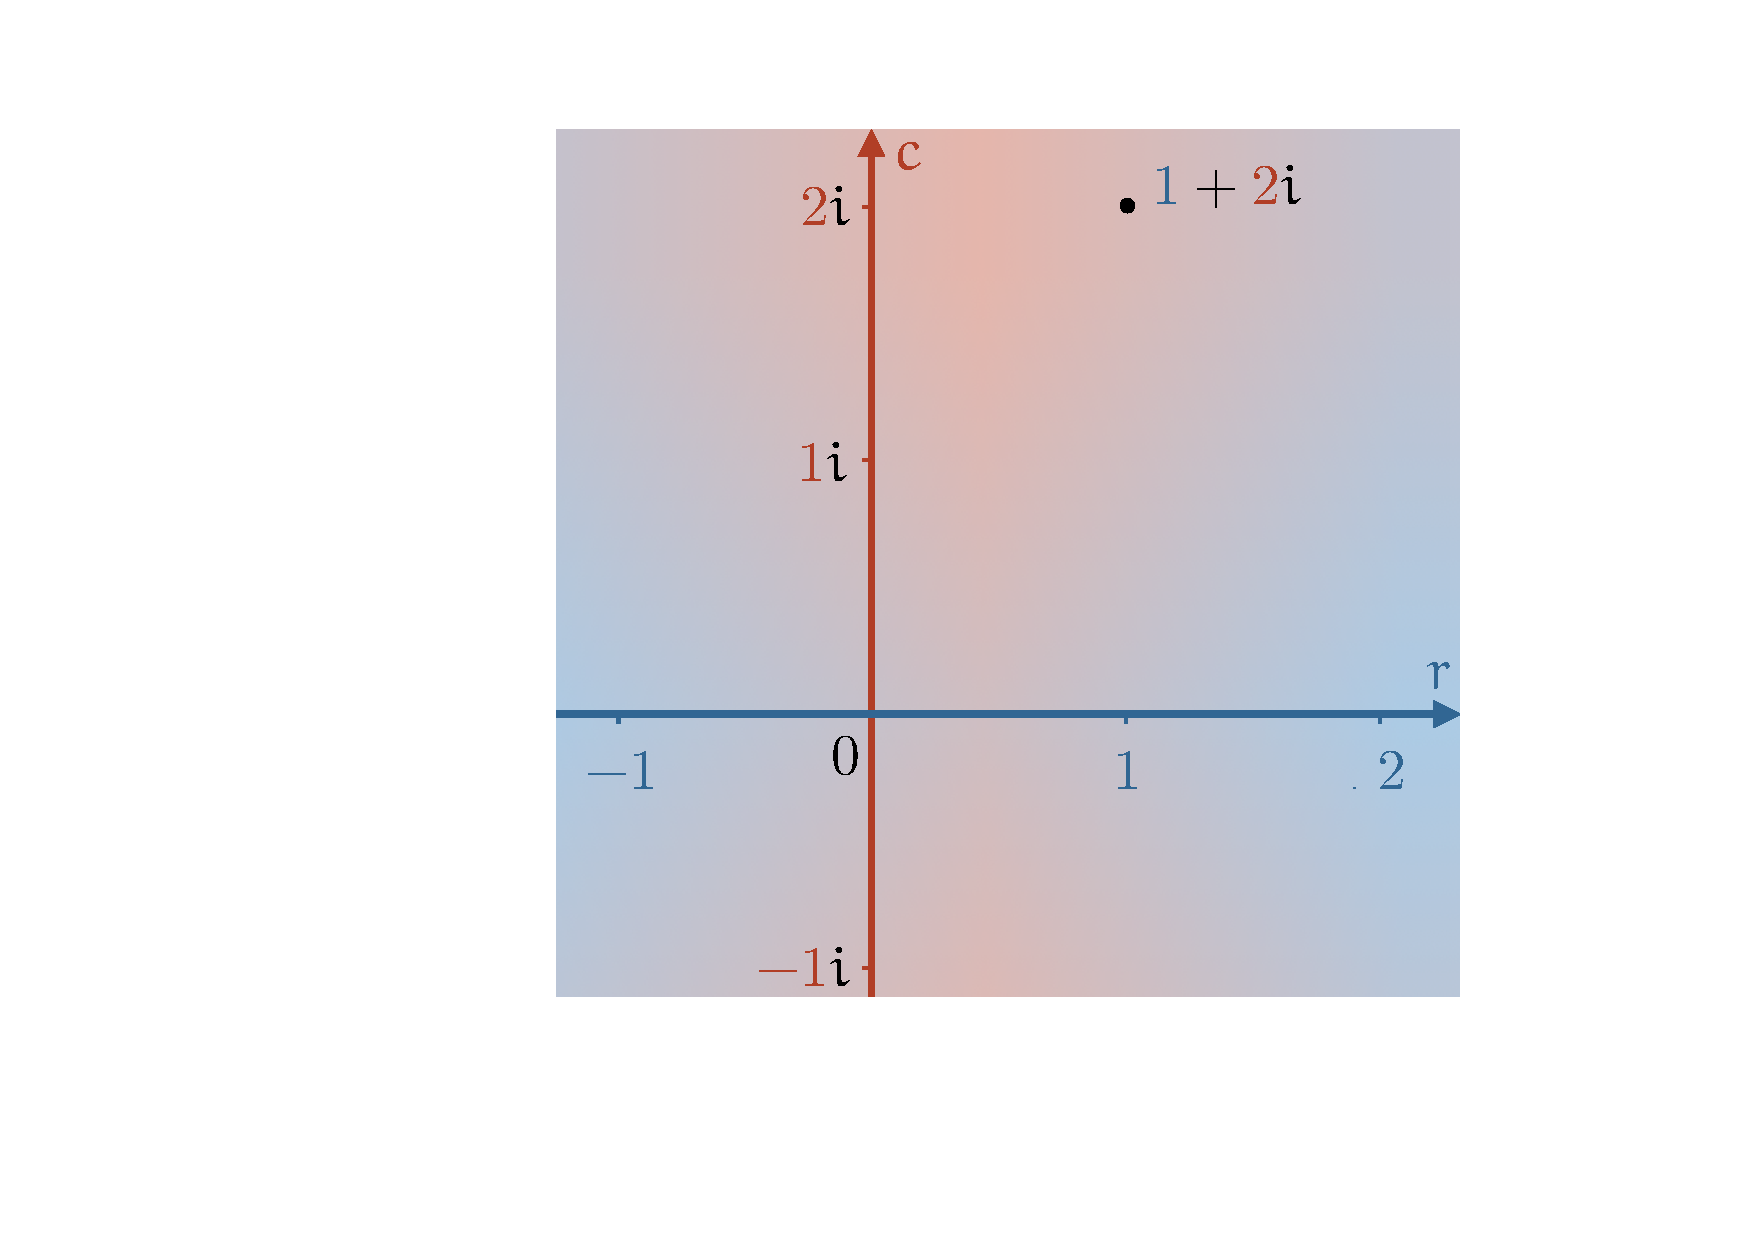
\includegraphics[width=0.7\textwidth]{./images/pca-3/complex-plane.pdf}
	}
\end{figure}

\index{Complex plane}

%<figure class="half center">
%<img src="/images/pca-3/complex-plane.svg">
%</figure>

The real-valued numbers that we already knew are a subset of the complex numbers: those complex number for which the \rc{imaginary part} is zero. In this picture, the real-valued numbers are on the \bc{horizontal axis}.

Note that this is just a visualization. There is nothing \emph{inherently} two-dimensional about the complex numbers, except that there is a very natural mapping from \(\mathbb C\) to \(\mathbb R^2\). At heart, it's just a set of numbers with a bunch of operations defined for them.

The nice thing about the mapping to the plane, however, is that we can take operations like multiplication, addition and so on, and see what they look like in this picture. This way, we can build a very helpful visual intuition for how the complex numbers behave.

Let's look at the most important concepts we'll need going forward. For addition, we can build on our existing intuitions. Adding two complex numbers works the same as adding two vectors in the plane: we place the tail of one on the head of the other.

\begin{figure}[H]
	\centerline{
		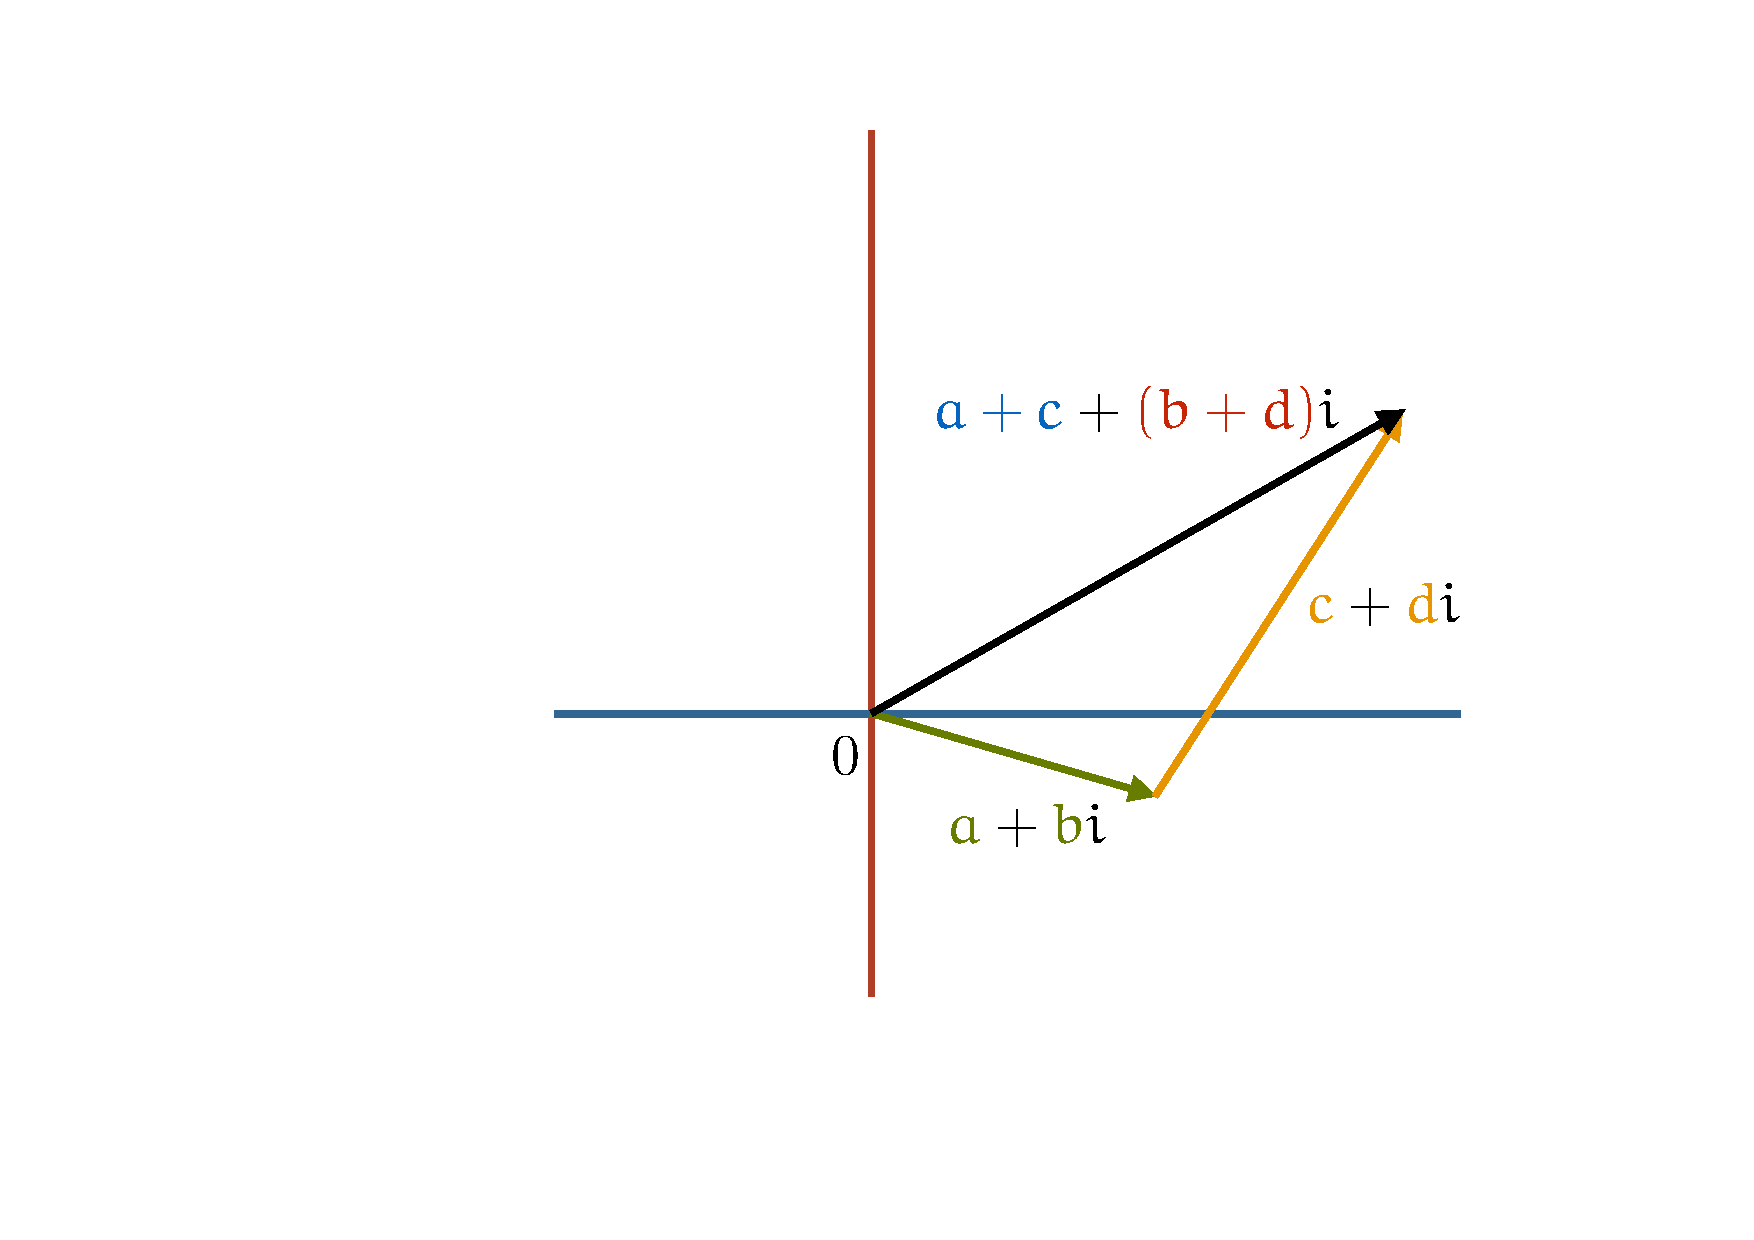
\includegraphics[width=0.7\textwidth]{./images/pca-3/addition.pdf}
	}
\end{figure}

%<figure class="half center">
%<img src="/images/pca-3/addition.svg">
%</figure>

The same logic shows that subtraction of complex numbers behaves as you'd expect. To compute \(x - y\), we subtract the real part of \(x\) from the real part of \(y\) and likewise for the imaginary part. Geometrically, this corresponds to vector subtraction in the plane.

\noindent To see what multiplication looks like, we can switch to a different way of representing complex numbers. Instead of giving the Cartesian coordinates \((\bc{r}, \rc{c})\) that lead to the number \(z = \bc{r} + \rc{c}i\), we use the \emph{polar} coordinates. We give an angle \(\gc{a}\) from the horizontal axis and a distance \(\gc{m}\) from the origin. The angle is also called the \emph{phase} and the distance is called the \emph{magnitude} or the \emph{modulus}. When we write a number like this, we'll use the notation \(z = \gc{m}\angle \gc{a}\). To refer to the magnitude of a complex number \(z\), which we'll be doing a lot, we use the notation \(|z|\).

\begin{figure}[H]
	\centerline{
		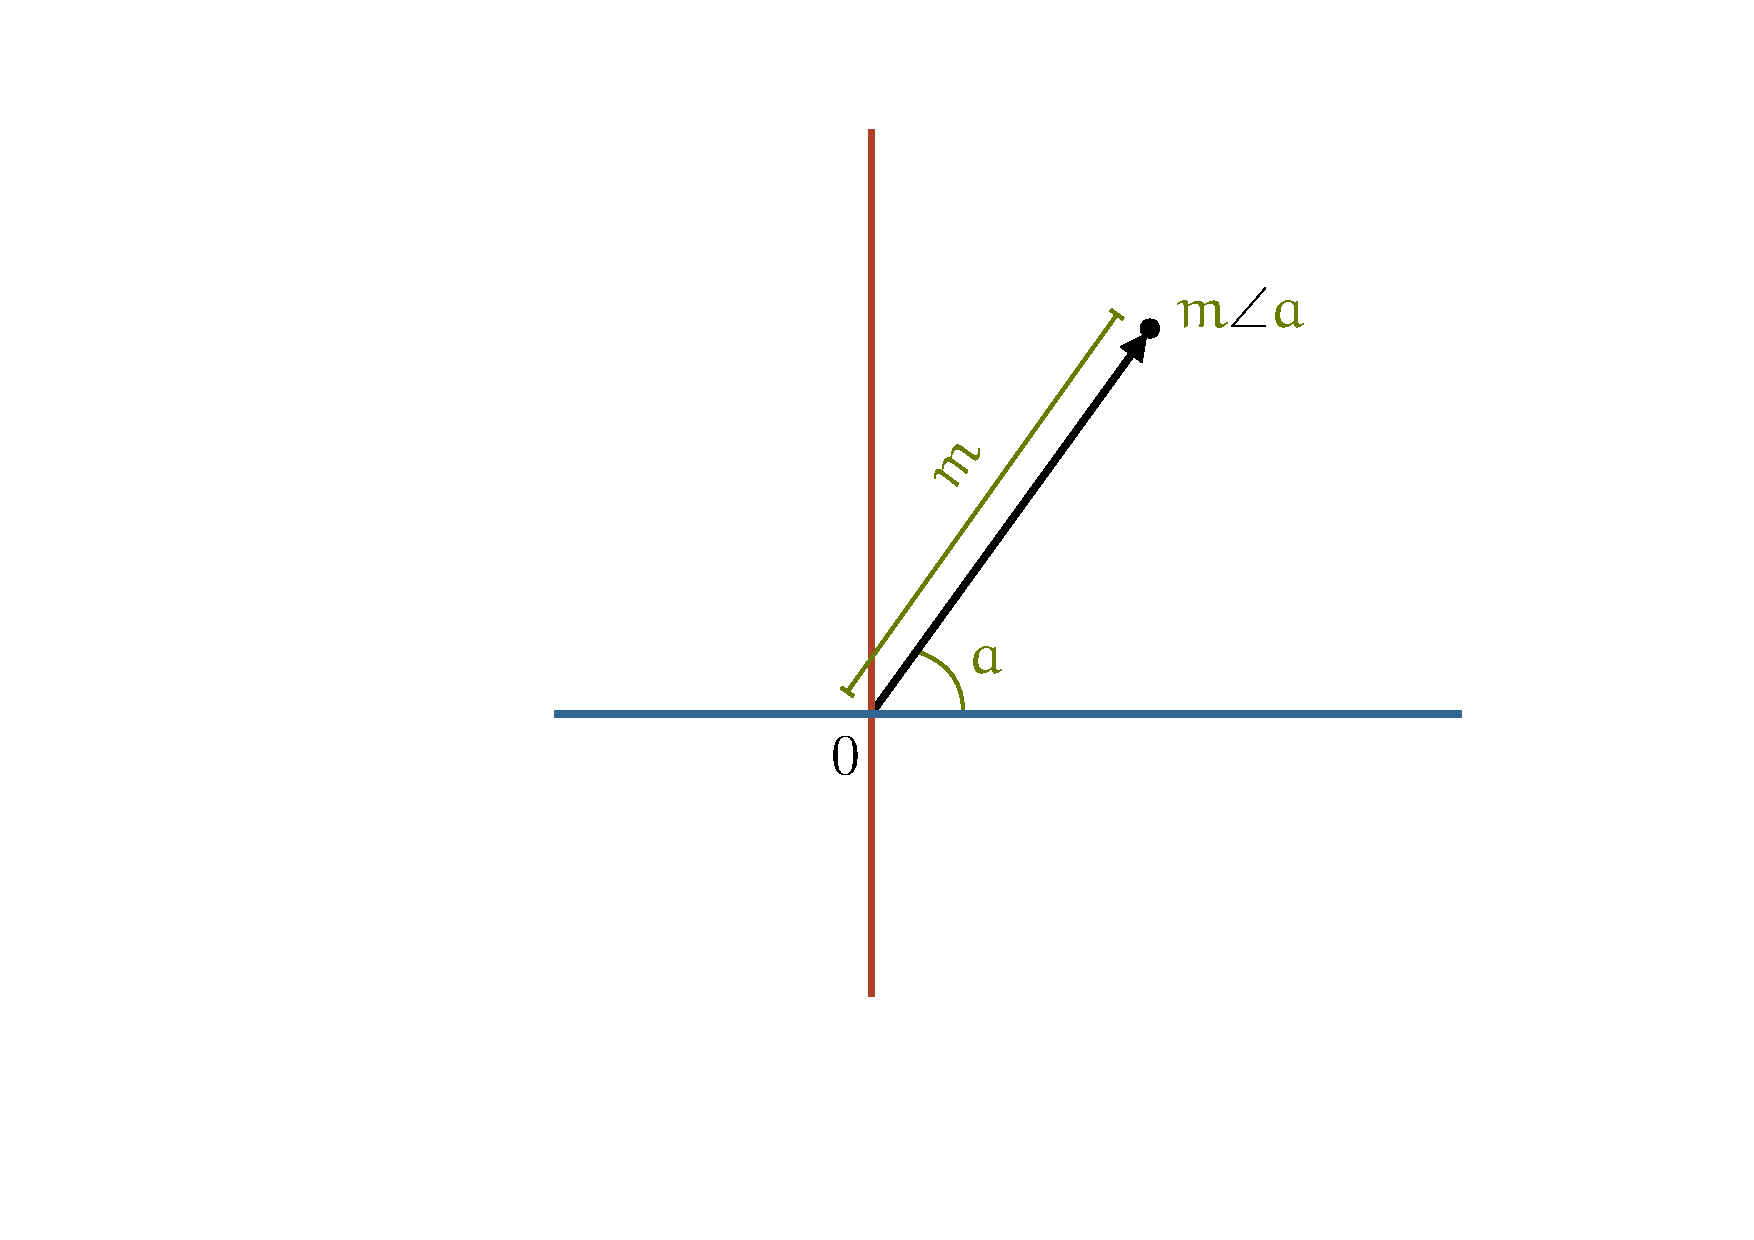
\includegraphics[width=0.7\textwidth]{./images/pca-3/polar.pdf}
	}
\end{figure}

%<figure class="half center">
%<img src="/images/pca-3/polar.svg">
%</figure>

 We call this representation of a complex number \emph{polar notation}, and the earlier representation \emph{Cartesian notation}.
 
 \index{Polar notation}\index{Cartesian notation}
 \index{Complex numbers!polar notation|textbf} \index{Complex numbers!Cartesian notation|textbf}

The reason polar notation is so useful, is that multiplication looks very natural in it. To see the relation, assume that we have a number \(z = \gc{m}\angle \gc{a}\). Then basic trigonometry tells us that in Cartesian notation, this number is written as \(z = \bc{\gc{m}\cos(\gc{a})} + \rc{\gc{m} \sin(\gc{a})} i\). 

\pagebreak
\noindent Let's see what happens if we take two numbers, in polar notation, and multiply them:

\begin{align*}
 & (\gc{m} \angle \gc{a})(\oc{n} \angle \oc{b})& \\
 &= (\gc{m}\cos(\gc{a}) + \gc{m} \sin(\gc{a}) i)\;(\oc{n}\cos(\oc{b}) + \oc{n}\sin(\oc{b}) i) \\
 &= \gc{m}\cos \gc{a} \;\oc{n} \cos \oc{b} + \gc{m} \sin \gc{a}\; \oc{n} \sin \oc{b} + (\gc{m} \cos \gc{a} \;\oc{n} \sin \oc{b}  + \oc{n}\cos \oc{b}\; \gc{m} \sin \gc{a})i \\
  &= \gc{m}\oc{n} (\cos \gc{a} \cos \oc{b} - \sin \gc{a} \sin \oc{b}) + \gc{m}\oc{n} (\cos \gc{a} \sin \oc{b} + \cos \oc{b} \sin \gc{a})i  \\
  &= \gc{m}\oc{n} \cos(\gc{a} + \oc{b}) + \gc{m}\oc{n} \sin(\gc{a} + \oc{b})i  \\
  &= (\gc{m}\oc{n}) \angle (\gc{a}+ \oc{b})
\end{align*}

In the third line, we apply the multiplication in Cartesian notation that we already worked out earlier. Then, in the fifth line, we apply some basic \href{https://en.wikipedia.org/wiki/List\_of\_trigonometric\_identities#Angle\_sum\_and\_difference\_identities}{trigonometric sum/difference identities}. 

What this tells us, is that when we view complex numbers in polar coordinates, multiplication has a very natural interpretation: the angle of the result is the \emph{sum} of the two original angles, while the magnitude of the result is the \emph{product} of the two original magnitudes.

\begin{figure}[H]
	\centerline{
		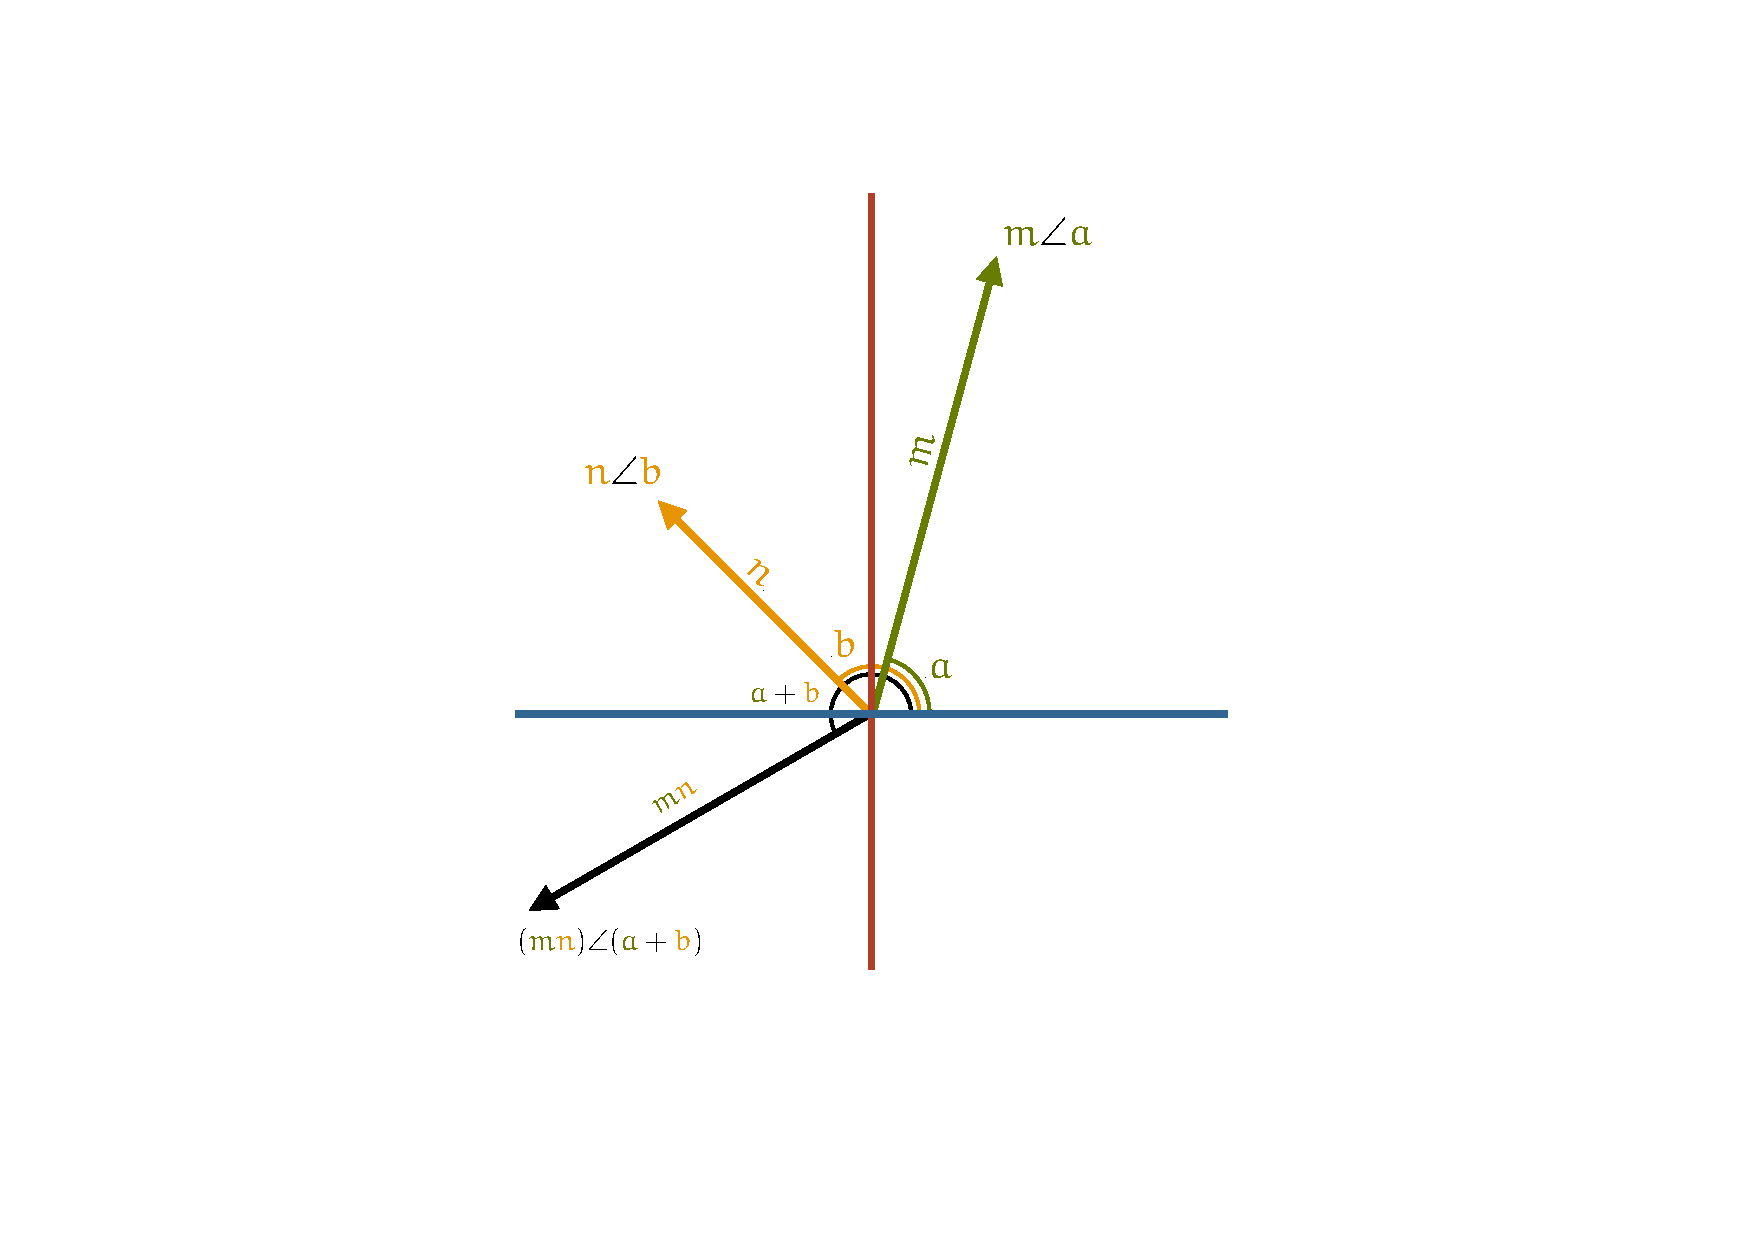
\includegraphics[width=0.7\textwidth]{./images/pca-3/multiplication.pdf}
	}
\end{figure}

%<figure class="half center">
%<img src="/images/pca-3/multiplication.svg">
%</figure>
%

The easiest way to define \emph{division} is as the operation that cancels out multipliciation. For each \(z\), there should be a \(z^{-1}\) so that multiplying by \(z\) and then by \(z^{-1}\) brings you back to where you were. Put simply \(zz^{-1} = 1\). Dividing by \(z\) can then be defined as multiplying by \(z^{-1}\). Using the polar notation, we can see that the following definition of \(z^{-1}\) does the trick:

\[z^{-1} = (\gc{m}\angle \gc{a})^{-1} = \frac{1}{\gc{m}}\angle -\gc{a} \p \]

Note how this view of multiplication agrees with special cases that we already know. For real numbers, the angle is always \(0\), and the magnitude is equal to the real value. Therefore, multiplying real numbers together reduces to the multiplication we already knew. 

The number \(i\) is written as \(1\angle90\deg\) in polar coordinates. That means that multiplying a number \(z\) by \(i\) keeps the magnitude of \(z\) the same, but rotates it by \(90\) degrees counter-clockwise. A real number multiplied by \(i\) is rotated from the \bc{horizontal} to the \rc{vertical} axis. If we multiply by \(i\) twice, we rotate \(180\) degrees, which for real numbers means negating them. This makes sense too, because \(z \cdot i \cdot i = z i^2 = z \cdot -1\).


\index{Complex numbers!exponentiation}

Which brings us to exponentiation. Raising complex numbers to arbitrary values, including to complex ones, is an important topic, but one which we can sidestep here. All we will need is the ability to raise a complex number to a natural number. That follows very naturally from multiplication:

\[
(\gc{m} \angle \gc{a})^n = (\gc{m} \angle \gc{a})(\gc{m} \angle \gc{a}) \ldots (\gc{m} \angle \gc{a}) = \gc{m}^n \angle n\gc{a} \p
\]

Again, let's look at some special cases. If the angle is \(0\), we stay on the real number line, and the operation reduces to ordinary exponentiation. If the magnitude is \(1\) but the angle is nonzero, then we rotate about the origin over the unit circle in \(n\) steps of angle \(\gc{a}\).

\begin{figure}[H]
	\centerline{
		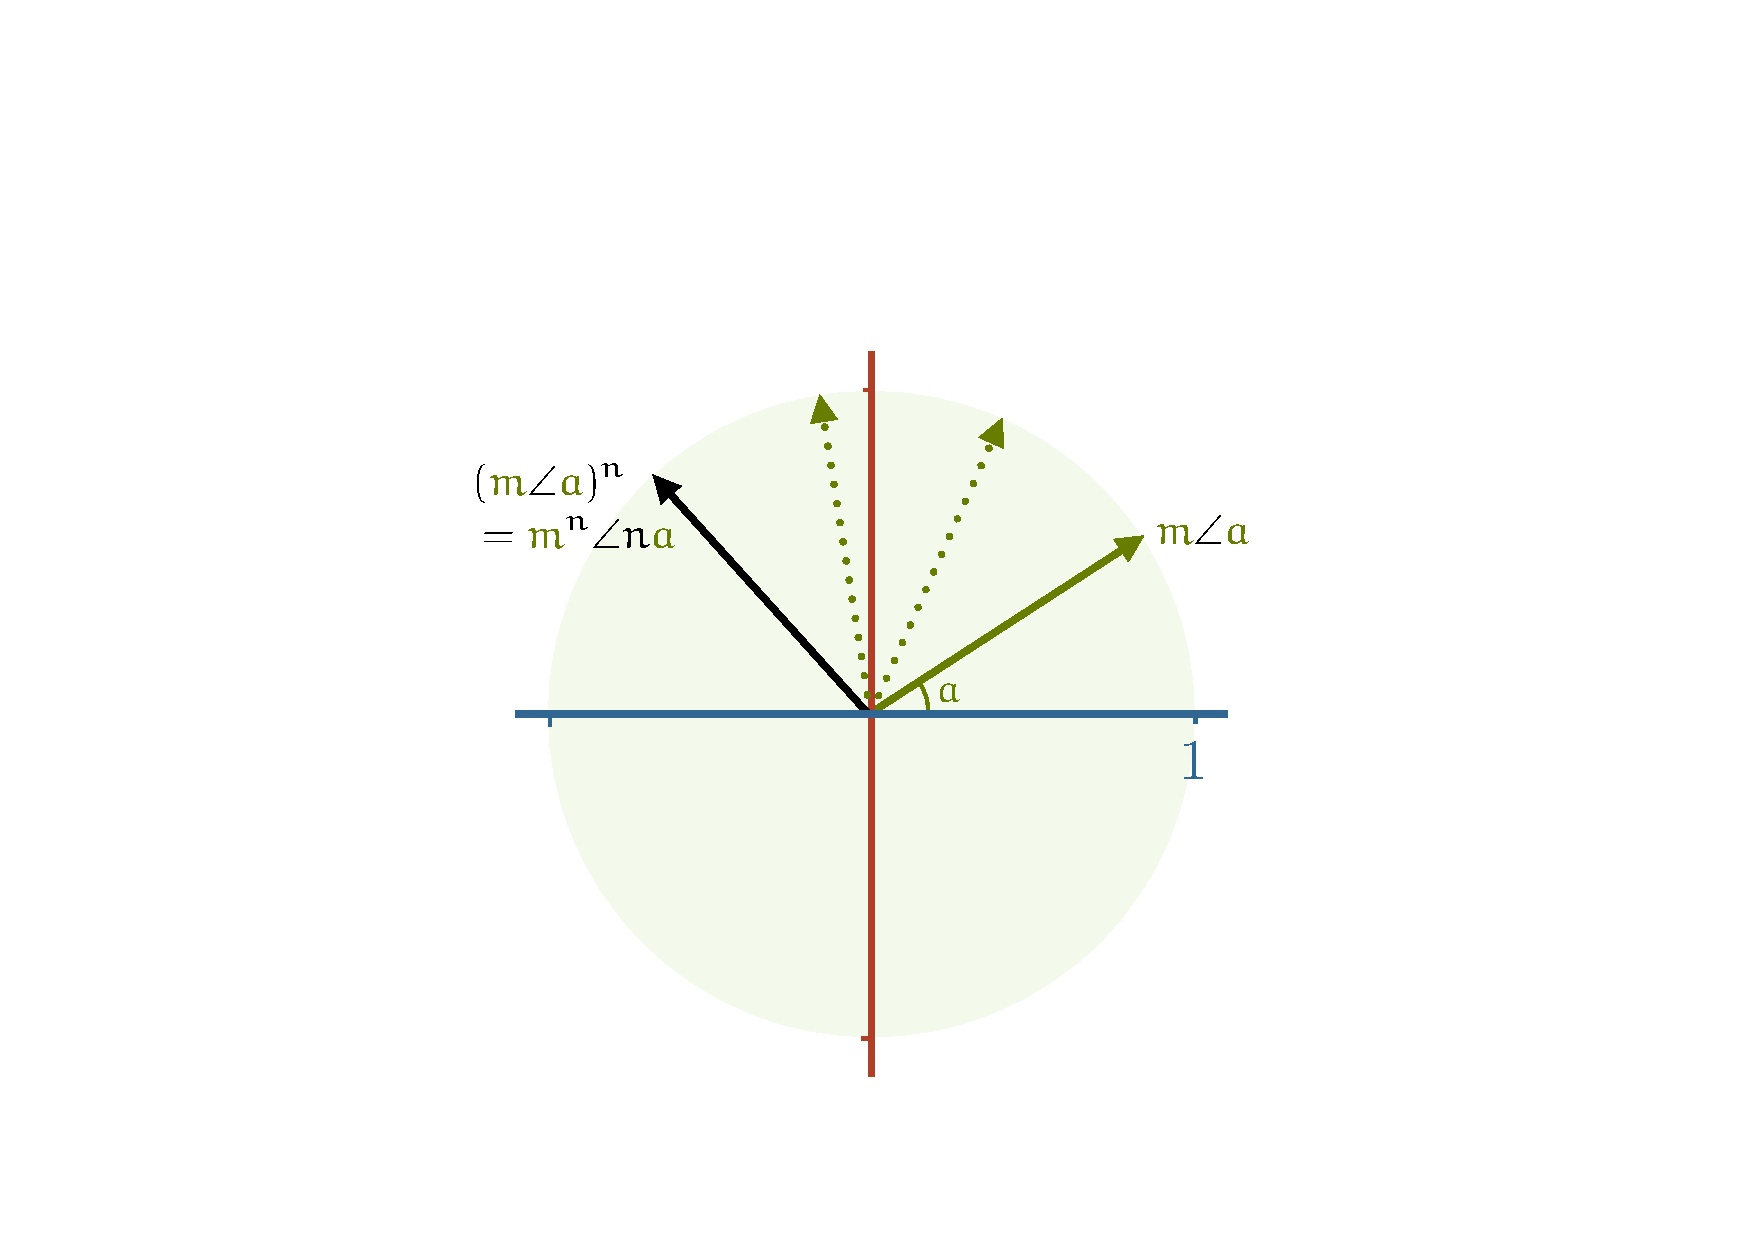
\includegraphics[width=0.7\textwidth]{./images/pca-3/exponentiation.pdf}
	}
\end{figure}

%<figure class="half center">
%<img src="/images/pca-3/exponentiation.svg">
%<figcaption>Exponentiation with unit magnitude.
%</figcaption>
%</figure>

The main thing we need, however, is not integer exponentiation, but its inverse: the \(n\)-th root. Given some complex number \(z = m\angle a\), which other number do we raise to the power \(n\) so that we end up at \(z\)? The answer follows directly from our polar view of the complex plane: the magnitude should be \(\sqrt[n]{m}\), which is just the real-valued \(n\)-th root, and the angle should be \(a/n\).

Let's check for \(\sqrt{-1}\), which started all this business. Which number should we raise to the power 2, so that we get \(-1\)? The magnitude of \(-1\) is \(1\), so our number has magnitude \(\sqrt{1} = 1\). Now we need a number with magnitude one, so that twice its angle equals \(180 \degree\). This is a \(90 \degree\) angle, so our number is \(1\angle 90\degree\), which is exactly where we find \(i\).

Notice how this solves the problem we had when we were constrained to the real line. Then we had negative numbers to deal with, and the real \(n\)-th root does not exist for negative numbers. Now, we are only ever applying the \(n\)-th root to \emph{magnitudes}, which are positive. The rest is dealt with by rotating away from the real numbers. This means that when it comes to complex numbers, we can always find some number that, when raised to \(n\), gives us \(z\). We call this the complex \(n\)-th root \(\sqrt[n]{z}\).

Note however, that this is not always a \emph{unique} number. Let's say we raise \(1\angle 10\degree\) to the power of \(4\). This gives us \(1\angle 40\degree\), so \(1\angle 10\degree\) is a fourth root of \(1\angle 40\degree\). However, if we raise \(1\angle 92.5\degree\) to the power of \(4\), we get \(1\angle 370\degree\), which is equal to \(1\angle 10\degree\) as well. Any angle \(a'\) for which \(a'\frac{1}{n}\,\text{mod}\;360 = a\) will give us an \(n\)-th root of \(m\angle a\). 

How many solutions does this give us for any given number? It's easiest to visualize this if we plot the \(n\)-th roots of 1.

\begin{figure}[H]
	\centerline{
		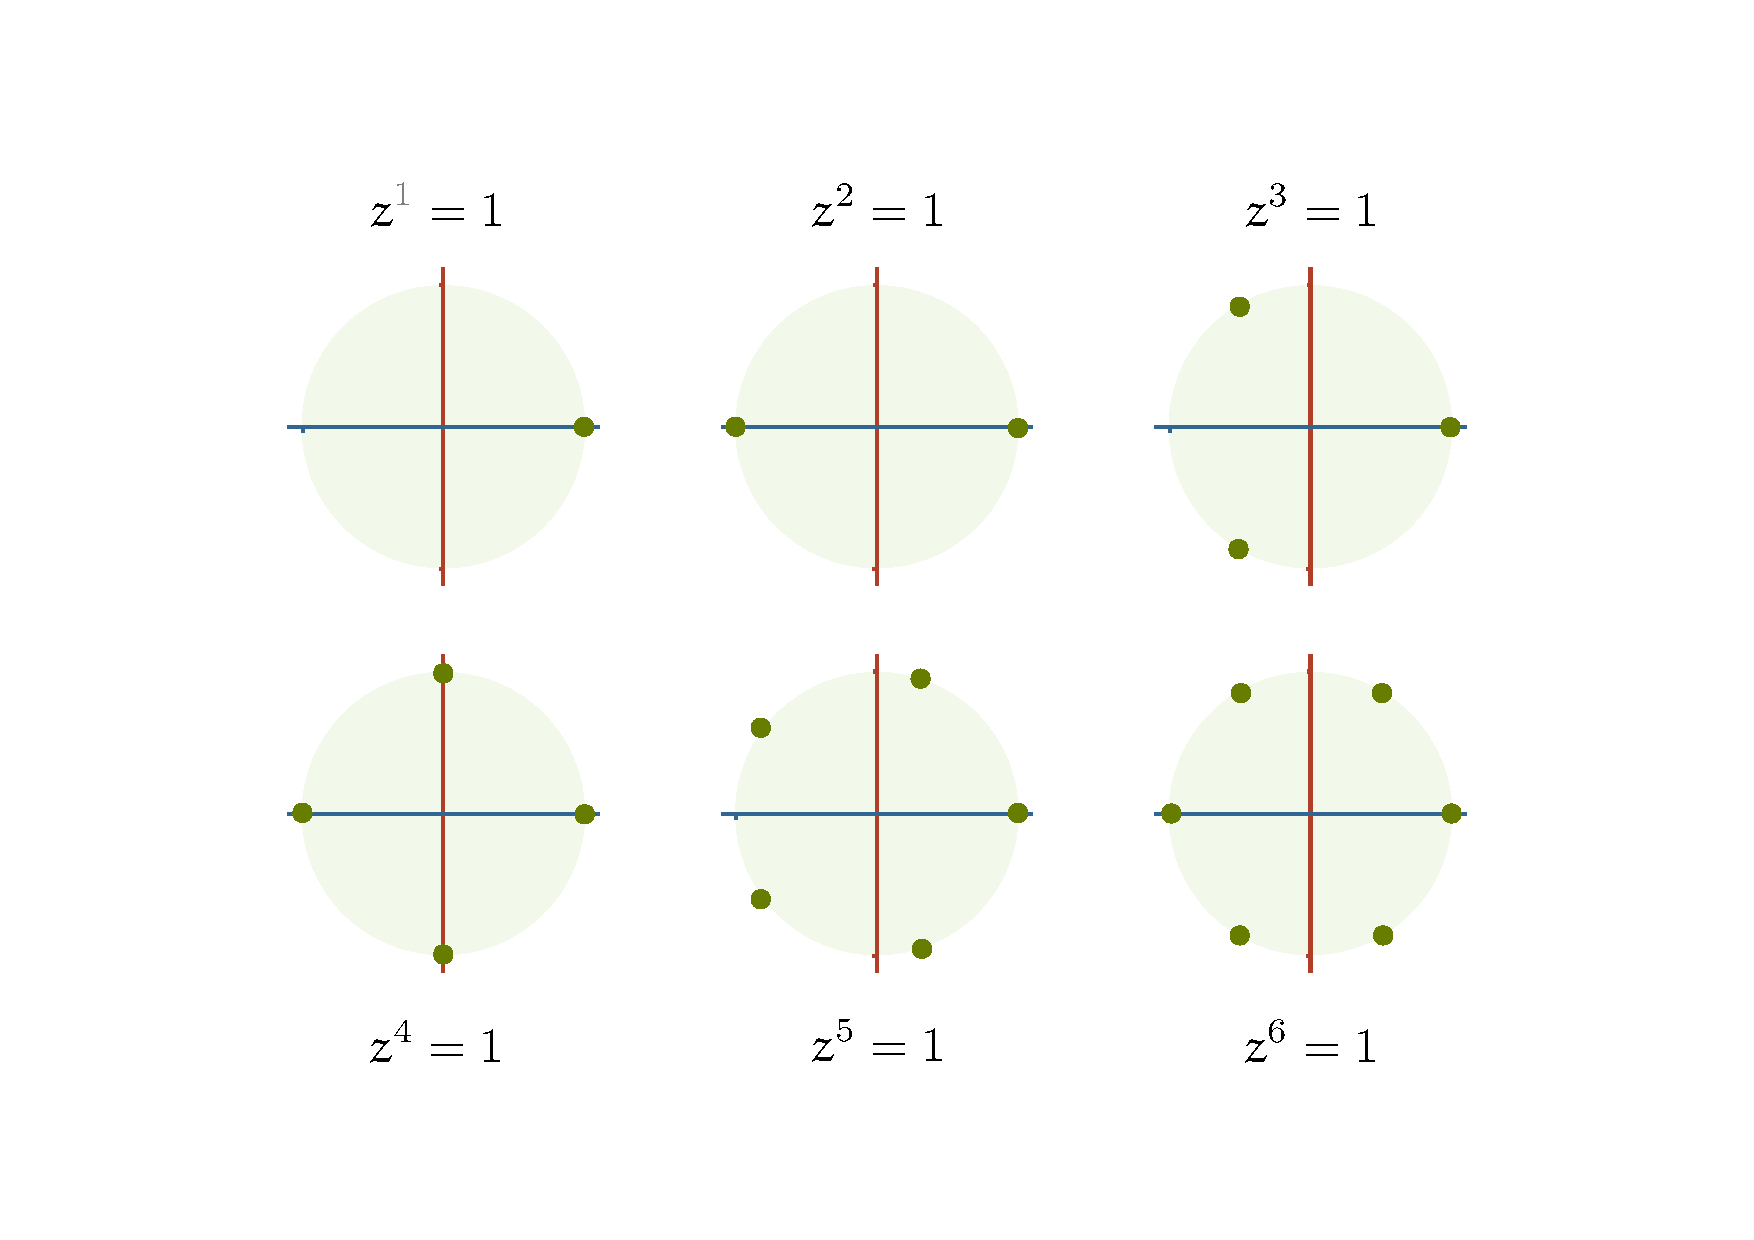
\includegraphics[width=1\textwidth]{./images/pca-3/nth-roots.pdf}
	}
\end{figure}

%<figure class="narrow">
%<img src="/images/pca-3/nth-roots.svg">
%</figure>

For each, of course, the real value \(1\) is a solution, but for the higher powers, there are additional solutions on the unit circle. For \(\sqrt[2]{1}\), for instance, multiplying \(-1\) by itself rotates it by 180 degrees to coincide with \(1\). For \(\sqrt[3]{1}\), we get three roots, two of which are non-real. The solution with angle \(120\deg\), when raised to the power of \(3\) gives us an angle of \(360\deg = 0\deg\). The solution with angle \(240\deg\) puts the angle after cubing at \(720 \deg = 0 \deg\). 

In short, every multiple of \(360\): \(0\), \(360\), \(720\), \(1080\), \(\ldots\), can be divided by \(n\) to give us a solution. Once we get to \(360n\), dividing by \(n\) gets us back to a solution we've already seen, so we get \(n\) unique solutions in total.

To translate this to roots of any complex number \(m\angle a\), we simply scale the circle so that its radius is \(\sqrt[n]{m}\) and then rotate it so that the first solution points in the direction of \(a/n\).

\begin{figure}[H]
	\centerline{
		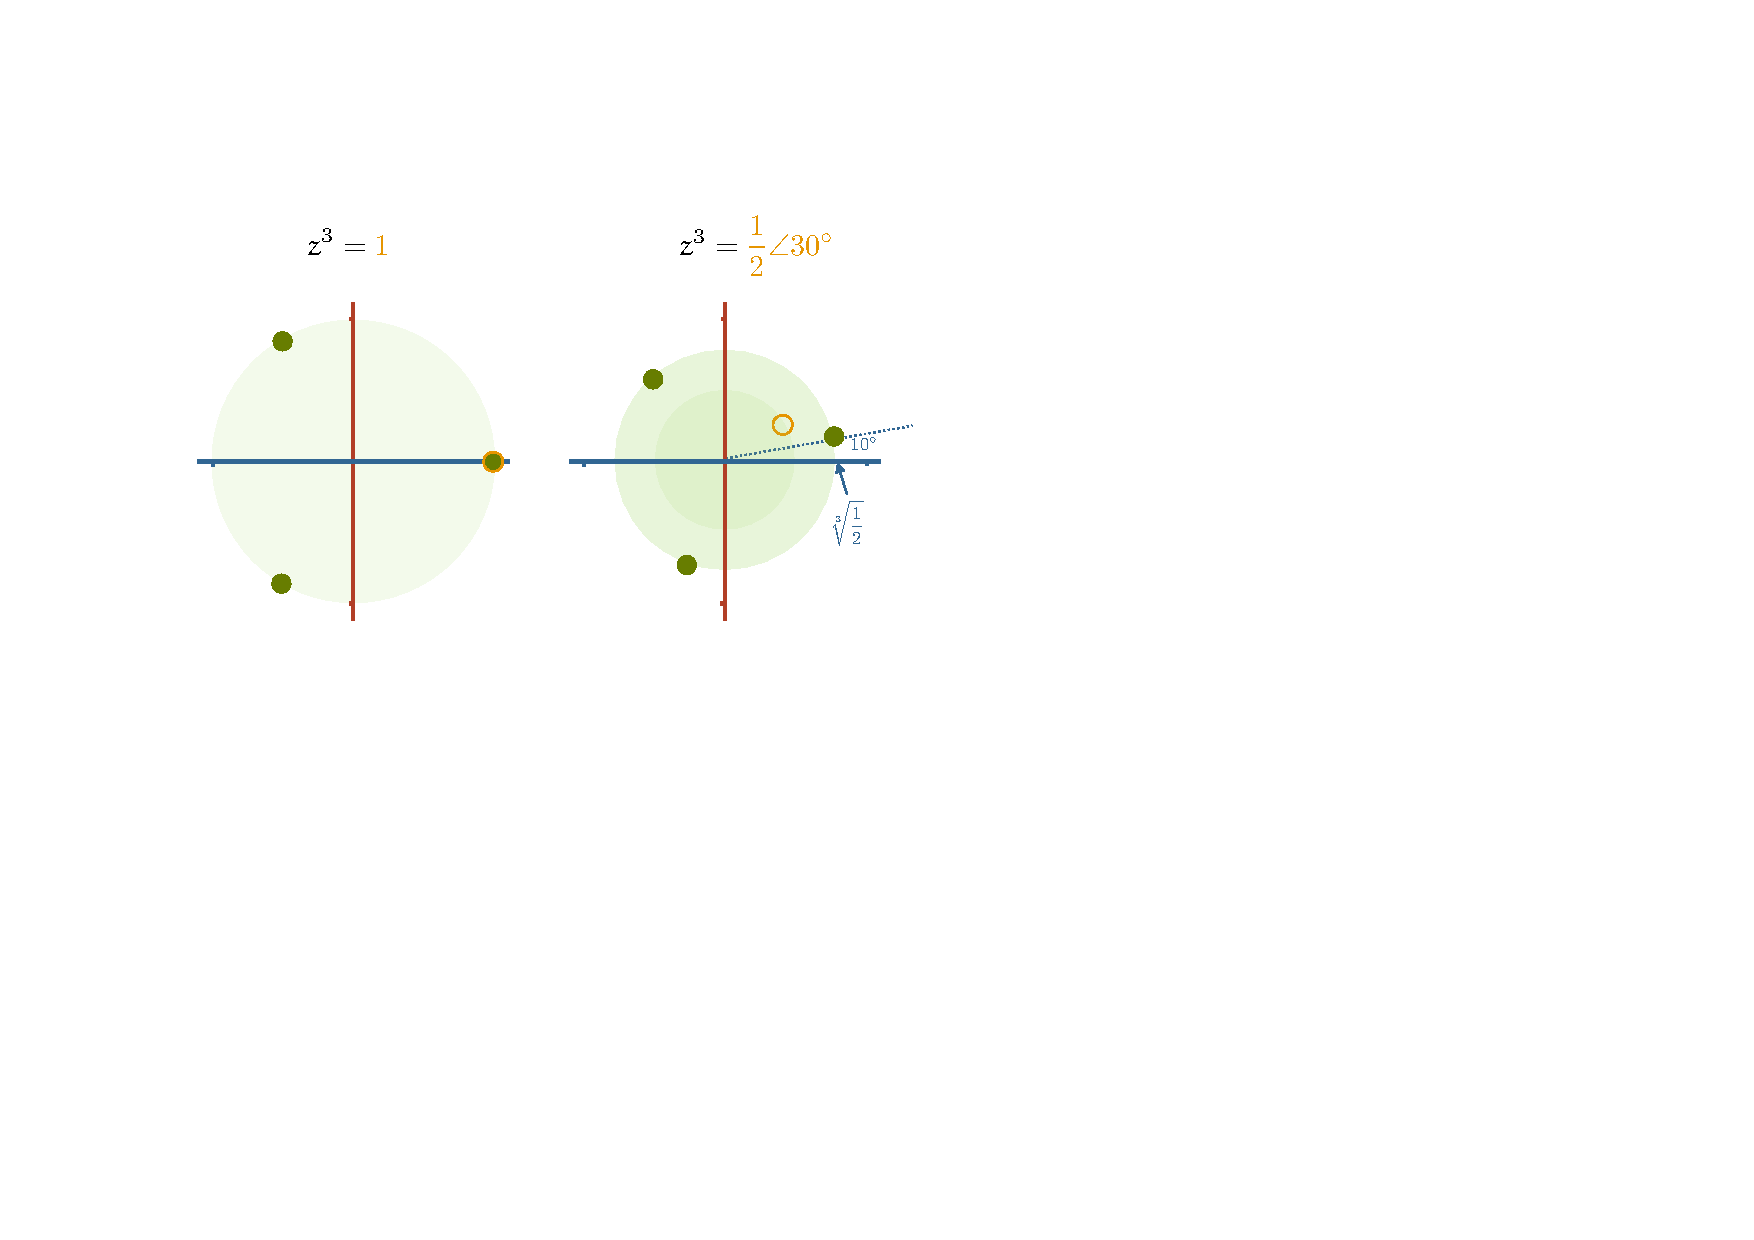
\includegraphics[width=1.05\textwidth]{./images/pca-3/general-root.pdf}
	}
\end{figure}

%<figure class="narrow">
%<img src="/images/pca-3/general-root.svg">
%</figure>

\section{The fundamental theorem of algebra}

The reason we are bringing in complex numbers, is that we are interested in talking, in general terms, about the roots of the chracteristic polynomial. When all we have access to are real-valued numbers, this becomes a messy and unpredictable business. A polynomial of order \(n\) can have anywhere between 0 and \(n\) roots. When we add complex numbers to our toolbelt, the whole picture becomes a lot simpler. And that is down to a result called \emph{the fundamental theorem of algebra}.

\index{Roots!of the characteristic polynomial}

The theorem has many equivalent statements, but this is the one most directly relevant to our purposes.

\begin{theorem}[The fundamental theorem of algebra] Any non-constant polynomial of order \(n\) has exactly \(n\) complex roots, counting multiplicities.
\end{theorem}

\index{Fundamental theorem of algebra|textbf}\index{Multiplicities}

\begin{aside}%
For now, don't worry about what is meant by multiplicities. We'll dig into that later. A constant polynomial is a function like \(f(x) = 3\), which will not have any roots.
\end{aside}

To prove this theorem, the first thing we need is to show that each such polynomial has \emph{one root}. After that, the rest is straightforward. So straightforward (to some) that this is often seen as an alternative statement of the fundamental theorem:

\begin{theorem}[\hspace{-0.15em}The fundamental theorem of  algebra (variant)] Any non-constant polynomial of order \(n\) has at least one complex root.
\end{theorem}

%<!-- 
%
%We'll first show that this holds for a subset of polynomials, which we'll call <em>simple polynomials</em>. That is, any polynomial of the form 
%
%\[
%p(z) = \bc{a}(z - \bc{b})^k + \bc{c}
%\]
%
%where \(k\) is a positive integer and \(\bc{a}\), \(\bc{b}\) and \(\bc{c}\) are arbitrary complex numbers, with \(\bc{a}\) non-zero.
%
%<div class="theorem"><strong class="gc">Lemma</strong> Any simple polynomial has at least one complex root.
%</div>
%<div class="proof"><p><em>Proof.</em> By simple algebraic manipulation, we get:
%\[\begin{align*}
% \bc{a}(z - \bc{b})^k + \bc{c} & = 0 \\
% z & = \sqrt[k]{-\frac{\bc{c}}{\bc{a}}} + \bc{b} \p
%\end{align*}\]
%This requires the operations of division, multiplication, addition and root taking. 
%
%We showed above that each of these always leads to another complex number (the complex numbers are <em>closed</em> under these operations), so the solution must exist in \(\mathbb C\).
%<span class="qed" /></p></div>
%
%The idea that we can take any integer root of any complex number is the fundamental building block of the theorem. From that, all we have to to is extend the idea to all polynomials. We do that by showing that locally, any polynomial can be well approximated by a simple polynomial. 
%-->

Let
\[
p(z) =\bc{c_n}z^n + \ldots + \bc{c_1}z + \bc{c_0}
\]

be our polynomial. For our purposes, we can think of the coefficients as real-valued, but the theorem holds for complex coefficients as well. The argument \(z\) and the result \(p(z)\) can always be complex.

To find a root of \(p\), we will consider the function \( |p(z)| \). That is, the magnitude of the complex number that we get out of \(p\). This provides the following benefits:

\index{Magnitude function}

\begin{itemize}
\item The magnitude is always non-negative. That means that the lowest possible value that \(|p(z)|\) can take on is \(0\), at which point we must have \(p(z) = 0\). In short, for a root of \(p(z)\), \(|p(z)|\) is both \(0\) and at a minimum.
\item Since the magnitude of a complex number is a single real value, \(|p(x)|\) is a function from two dimensions (the complex plane) to one dimension (the reals) and we can easily visualize it in three dimensions. This is not so easy for \(p(x)\) itself, since we have a two-dimensional input \emph{and} a two-dimensional output.
\end{itemize}

%<!-- 
%
%Our big shortcut in this proof will be to look at what this polynomial does in the extreme cases: when its input is very far from 0, and when it's input is very close to zero. Let's start by looking at real-valued polynomials of the from \(x^n\). Consider the following plot.
%
%What we see is that if \(x\) is larger than 0 \(x^3\) grows much quicker than \(x^2\). The distance between them \(x^3 - x^2\) clearly grows unbounded: if you give me any number \(b\), I can give you a number \(x\) for which the difference between the two is larger than \(b\). This means that in a real valued polynomial of degree \(n\), the \(x^n\) term <em>dominates</em>. For large enough inputs, it's bigger than all the other terms put together. At that point, we know that if \(\bc{c_n}x^n\) is bigger than \(0\), so is \(p(x)\).
%
% - diagram
%
%The same holds for complex-valued polynomials. Here, each term is essentially a vector in the complex plane, all of which we're adding together. The magnitude of each of these vectors is the magnitude of the input raised to some power. The influence of the highest-degree term is kept down the most if all the other terms have vectors pointing in the exact opposite direction to it. This puts all vectors on one line, which bring us back to the previous diagram.
%
% - diagram
% 
% -->

Our big shortcut in this proof will be to look at what the magnitude does in extreme cases: for very large inputs, and for inputs very close to the minimum. We will see that in both cases, the function can be approximated well by the magnitude of a simple polynomial. 

To see this, let's start with a simple real-valued example. The polynomial \(p(x) = \rc{x^3} + \bc{x^2} + \gc{x}\) in the positive range. In this area, \(p(x)\) is equal to its magnitude, so we don't need to worry about the distinction yet.

\vspace{-1em}
\begin{figure}[H]
	\centerline{
		\includesvg[width=1\textwidth]{./images/pca-3/real-polynomialmedium.svg}
	}
\end{figure}
\vspace{-1em}

%<figure class="narrow">
%<img src="/images/pca-3/real-polynomialmedium.svg">
%</figure>

\noindent What we see here, is that as \(x\) gets bigger, the term \(\rc{x^3}\) dominates. Almost all the contribution to the magnitude comes from this term, and pretty soon, the simpler polynomial \(\rc{x^3}\) becomes a pretty good approximation of the polynomial \(\rc{x^3} + \oc{x^2} + \bc{x}\). This is not surprising, since \rc{the cube} grows much faster than \oc{the square} which grows much faster than \bc{the identity}.

Toward \(x=0\), where \(p\) has a minimum, the opposite happens. As \(\rc{x^3}\) grows the fastest when \(x > 1\), so it \emph{shrinks} the fastest when \(0 < x < 1\). In this regime the term that shrinks the slowest, \(\bc{x}\) begins to dominate, and \(\bc{x}\) becomes a good approximation of the function \(p\).

\enlargethispage{3em}

Of course, this is just one polynomial. If we move to complex polynomials, and we allow for any order and all possible coefficients, does this pattern still hold? Let's imagine a generic complex polynomial. In this case, all terms in the polynomial are complex numbers, and the value of the polynomial is their sum.

\vspace{-1em}
\begin{figure}[H]
	\centerline{
		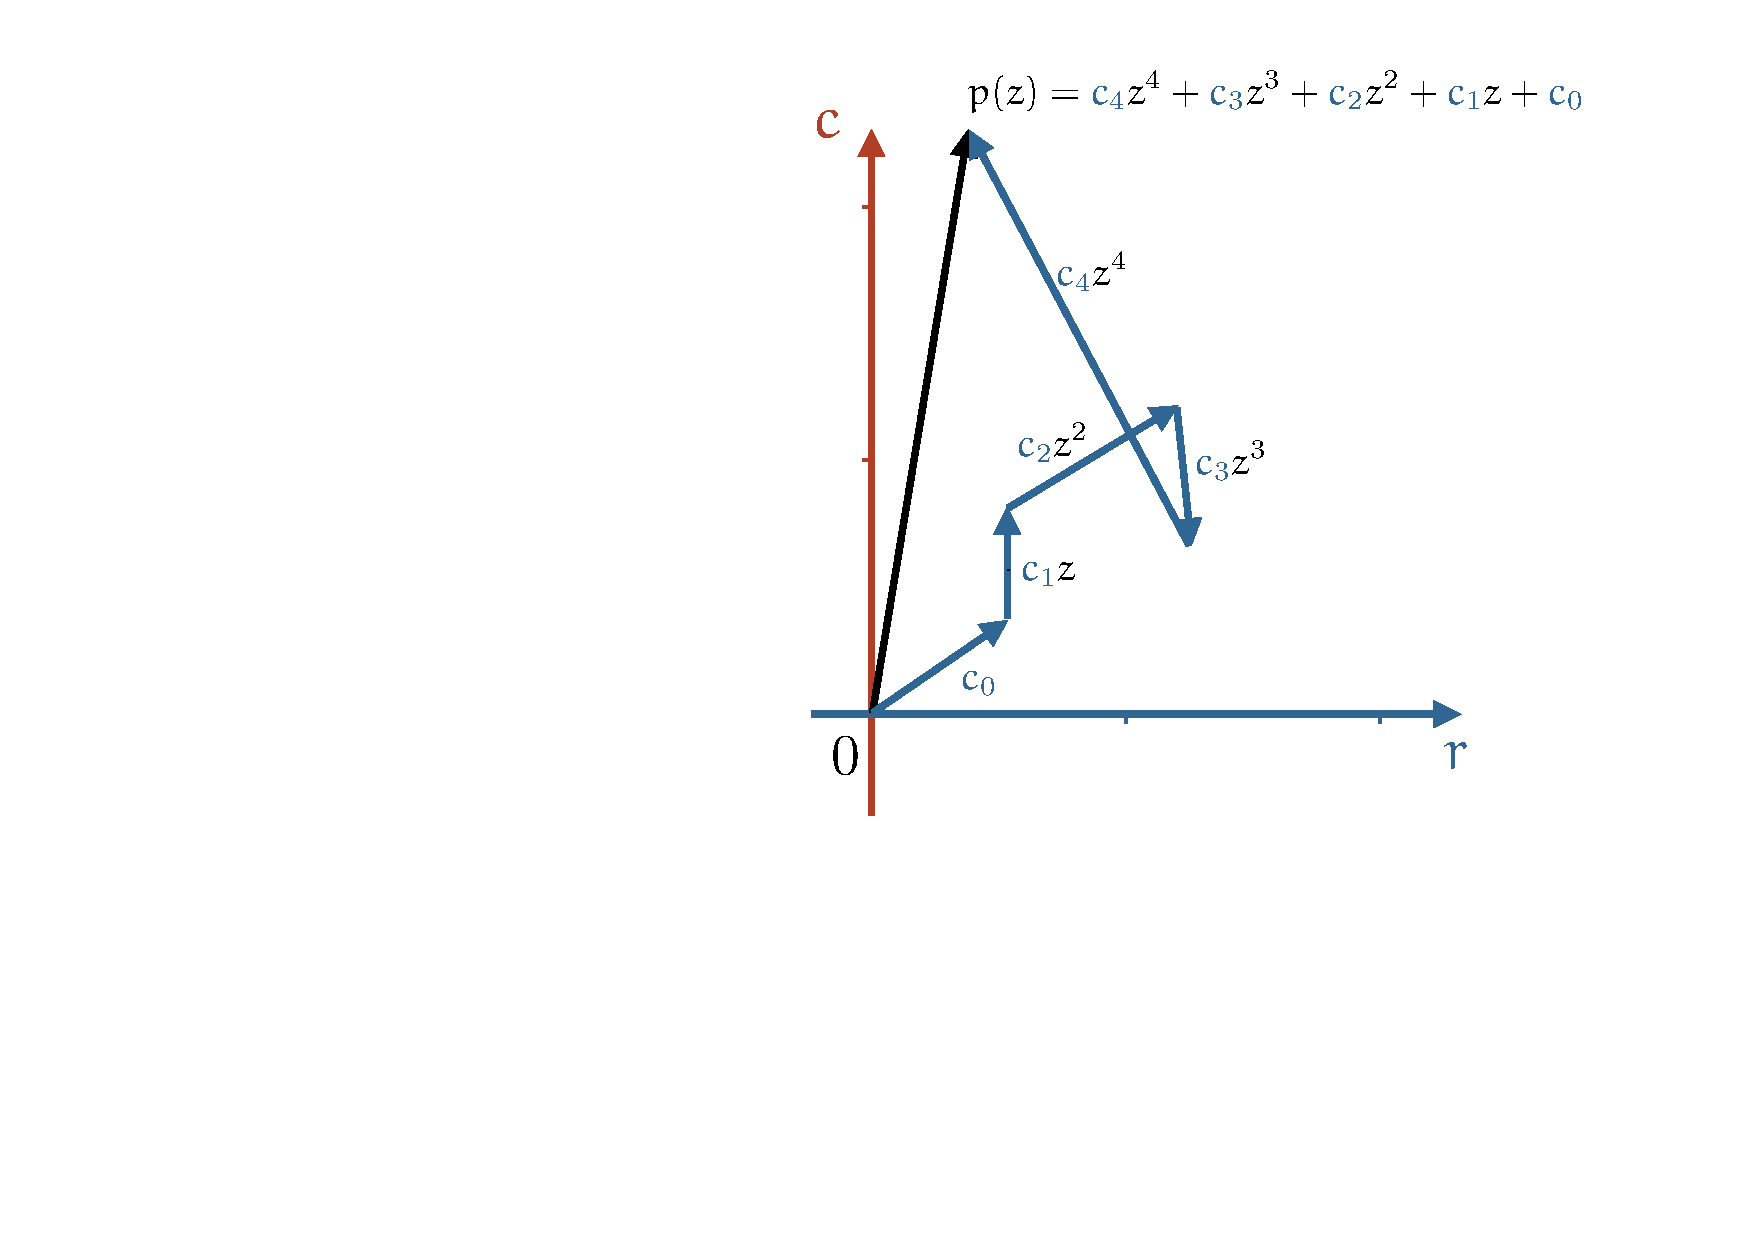
\includegraphics[width=0.6\textwidth]{./images/pca-3/polynomial-terms.pdf}
	}
\end{figure}
\vspace{-1em}

\index{Dominant terms of a polynomial}\index{Polynomial!dominant terms of}

%<figure class="tile4 centering">
%<img src="/images/pca-3/polynomial-terms.svg">
%</figure>

\noindent The magnitude \(|p(z)|\) of the polynomial at \(z\) is the distance of the end result to the origin. Each term contributes to this magnitude in a different direction. If we want to show that a particular term dominates, we can look at the worst case: that term points in one direction, and all other terms point in the exact opposite direction.

\begin{figure}[H]
	\centerline{
		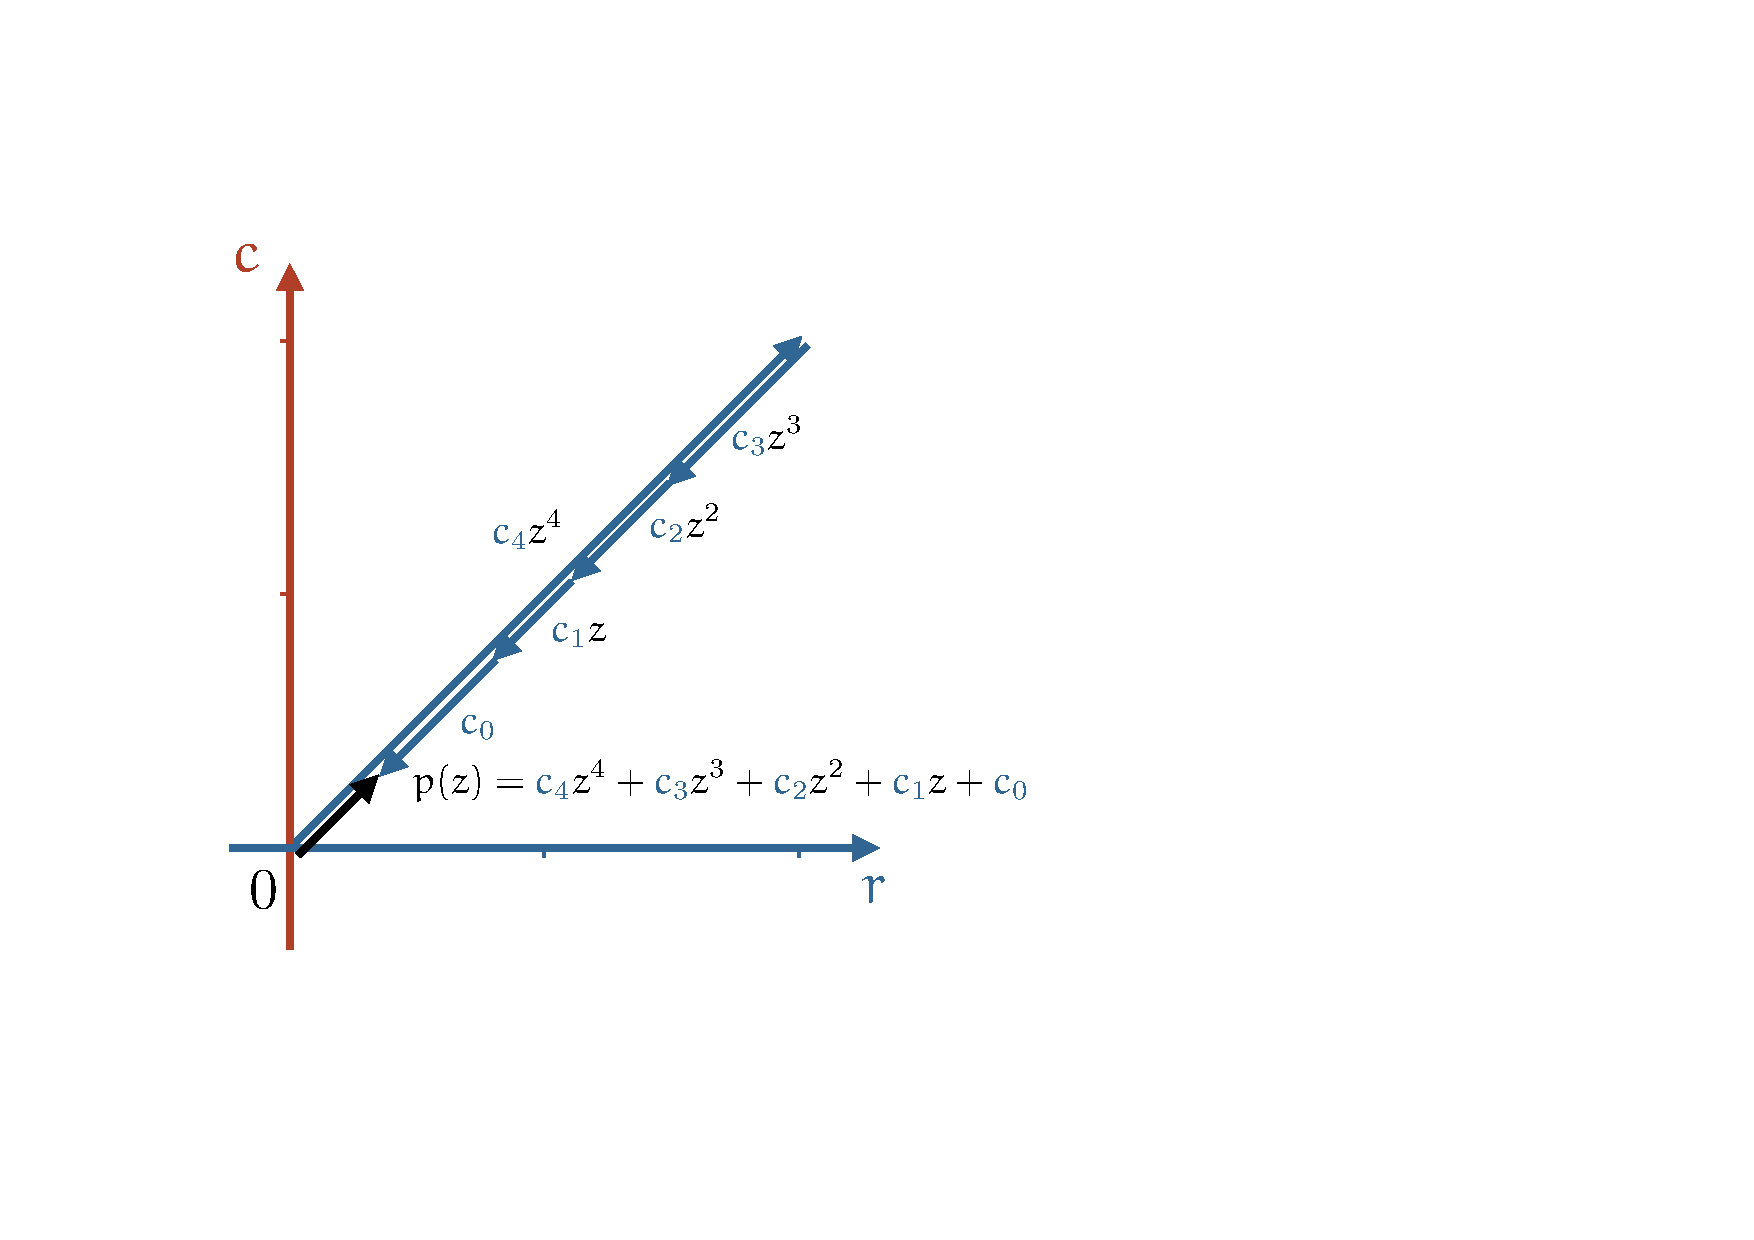
\includegraphics[width=0.6\textwidth]{./images/pca-3/term-domination.pdf}
	}
\end{figure}

%<figure class="tile4 centering">
%<img src="/images/pca-3/term-domination.svg" class="third">
%<figcaption>To show that the term \(\bc{c_4}z^4\) dominates, we can assume that all other terms point in the opposite direction. If the remainder of this term minus the others is still close to the magnitude of \(p(z)\), this will also be true when the other terms point in other directions.</figcaption>
%</figure>

In this case, we can ignore the angles of the terms and focus only on their magnitudes. If we assume the highest-order term points in the opposite direction of the rest, the total magnitude is

\begin{align*}
|p(z)| &= \left |\bc{c_{n}} {z}^n\right| - \left|\bc{c_{n-1}} {z}^{n-1}\right | - \ldots - \left |\bc{c_{1}} z\right | - \left |\bc{c_{0}}\right| \\
& = |\bc{c_{n}}| {|z|}^n - |\bc{c_{n-1}}| {|z|}^{n-1} - \ldots - |\bc{c_{1}}| |z| - |\bc{c_{0}}|
\end{align*}

\begin{aside}Note that the terms we are subtracting are all magnitudes, so they are all positive.\end{aside}

We will first use this to show that \(|p(z)|\) has some definite minimum. One alternative situation would be if \(p(z)\) is a function that is positive everywhere and monotonically increasing in some direction, like \(e^x\) is on the real number line. We'll need to exclude such possibilities first.

Assume that \(|z| > 1\) for some \(z\). If so, we make the total value of the sum \emph{smaller} if we replace all lower-order powers by \(z^{n-1}\). This means that

\begin{align*}
|p(z)| &> |\bc{c_{n}}| {|z|}^n  - |\bc{c_{0}}| - \sum_{i\in 1..n-1} |\bc{c_{i}}| {|z|}^{n-1} \\
 &= |\bc{c_{n}}| {|z|}^n - |\bc{c_{0}}| - {|z|}^{n-1}\sum_{i\in 1..n-1} |\bc{c_{i}}| \\
 &= {|z|}^{n-1} \left (|\bc{c_n}| {|z|} - \sum_{i\in 1..n-1} |\bc{c_{i}}|\right) - |\bc{c_0}|
\end{align*}

If we choose \(z\) so that its magnitude is larger than \(\frac{1}{|\bc{c_n}|} \sum_i |\bc{c_i}|\), the factor in brackets becomes positive. Beyond that, we know that there is some value of \(|z|\) large enough that the first term is bigger than the second. In short, for a suffciently large \(B\), we can always choose a value of \(z\) such that \(|p(z)|\) is larger than \(B\).

This means we can draw some large circle with radius \(R\), find the smallest value of \(|p(z)|\) inside the circle, and then draw a second circle with radius \(B\) so that all values outside of \(p(z)\) outside the second circle are larger than this minimum inside the first circle. This means \(|p(x)|\) has a definite minimum inside the second circle.

Now, all we need to do is show that this minimum can be expressed by a complex number. To do that, we'll follow the same sort of argument, but with the magnitude going to \(0\), so that the \emph{lower-order} terms dominate.

First, let \(z_0\) be the minimum we've just shown must exist. Translate \(p\) so that this minimum coincides with the origin, and call the result \(q(z)\). Specifically, \(q(z) = p(z - z_0)\).

This is another \(n\)-th order polynomial. We'll call its coefficients \(\bc{d_i}\). Note that \(q(0)\) has the same value as \(p(z_0)\) by construction. What we want to show is that \(p(z_0) = 0\).

In many polynomials the lowest-order term is the first-order term \(\bc{c_1}z\). However, we need to account for cases where this term is always zero. To be general, we write \(q\) as
%
\[
q(z) = \bc{d_0} + \bc{d_k}z^k + \bc{d_{k+1}}z^{k+1} + \;\ldots\; + \bc{d_n}z^n
\]

where \(k\) is the order of the lowest-order, non-constant term.

\noindent We'll show that the proportion of the sum contributed by the higher order terms vanishes as we get near zero, so we can take the simpler function \(q'(z) = \bc{c_0} + \bc{c_k}z^k\) as a good approximation, that becomes perfect at the origin.

\begin{aside}
Note that \(q(0) = q'(0)\).
\end{aside}

More formally, lets look at the ratio between the higher-order terms and the \(k\)th-order term:

\[
r = \frac{  |\bc{d_{k+1}}||z|^{k+1} + \;\ldots\; + |\bc{d_n}||z|^n  }{  |\bc{d_{k}}||z|^k } \p
\]

Assuming that \(|z| < 1\), the numerator is made bigger by reducing all exponents to \(z^{k+1}\), so 

\[
r < \frac{  |z|^{k+1} \sum_{i\in k+1..n} |\bc{d_i}| }{  |\bc{d_{k}}||z|^k } = |z|\frac{   \sum_{i} |\bc{d_i}| }{  |\bc{d_{k}}| } \p
\]

The second factor is a constant, so if we want to make the contribution of the higher order terms less than some given \(\epsilon\), we just need to choose a \(z\) with small enough magnitude.

\begin{aside}Specifically \(|z| < \epsilon \frac{ |\bc{d_k}| }{ \sum_i |\bc{d_i}|}\). Fill this into the above, and note that the two fractions cancel out, leaving only \(\epsilon\).
\end{aside}

This allows us to continue our analysis with \(q'\) instead of \(q\). Next, we can show that because \(|q'(z)|\) has a minimum at \(0\), that minimum must be equal to \(0\), so that \(\bc{d_0} = 0\).

At first, this may not be obvious. Why should a function \(q'(z) = \bc{c_k}z^k + \bc{c_0}\) necessarily have \(\bc{c_0} = 0\) if its magnitude has a minimum at \(0\)? It becomes clearer if we take the image of the roots of \(z^n -  1\) that we showed earlier, and create a 3d plot of the corresponding magnitude functions \(|z^n - 1|\).

\begin{figure}[H]
	\centerline{
		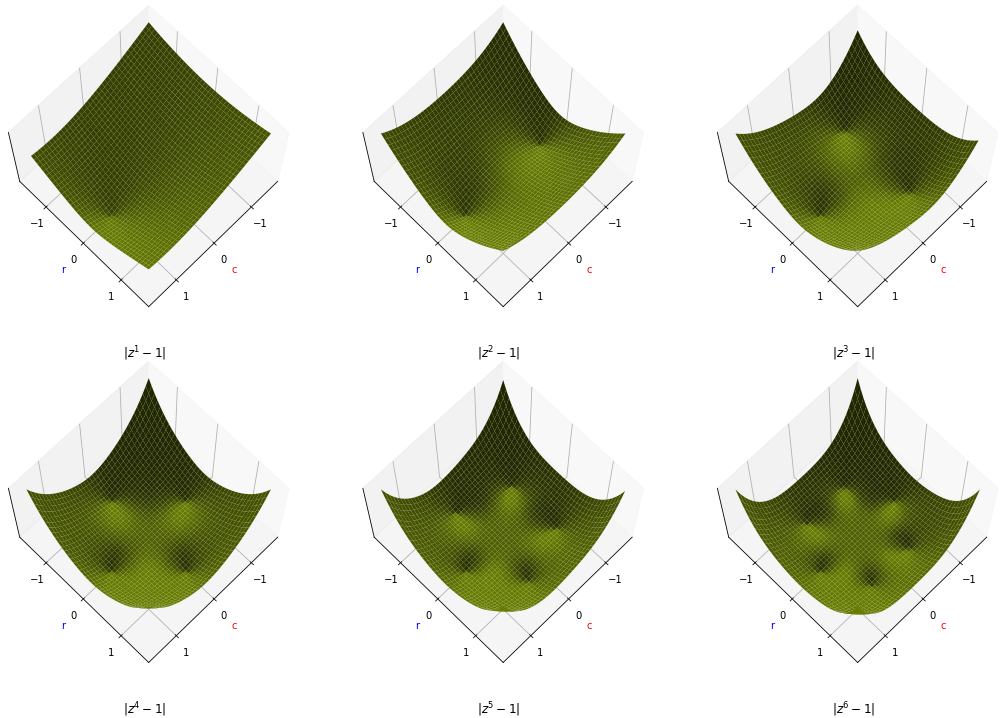
\includegraphics[width=1.1\textwidth]{./images/pca-3/roots-3d.png}
	}
\end{figure}

%<figure class="wide centering">
%<img src="/images/pca-3/roots-3d.png" class="three-quarters">
%</figure>

This kind of picture applies to the more general function \(|\bc{c_k}z^k + \bc{c_0}|\) as well: the two constants rotate the image and change how close the roots are to the origin, but unless \(\bc{c_0} = 0\), we get a ring of roots some distance from the origin and no root at the origin. This contradicts what we know: that \(|q(z)|\) has a minimum at 0, so we know that \(c_0\) must be \(0\).

To prove this formally, let \(z = \sqrt[k]{-\bc{d_0}/\bc{d_k}}\), one of the roots of \(q'\) , and let \(\epsilon\) be some real value near 0. Then we have:

\begin{align*}
|q'(\epsilon z)| &= |\bc{d_0} + \bc{d_k} \cdot - \epsilon^k \frac{\bc{d_0}}{\bc{d_k}}|  \\
&= |\bc{d_0} - \epsilon^k \bc{d_0}|
\end{align*}

Note that both terms in this last line point in the same direction, so if \(\bc{d_0} >0\), the resulting magnitude is smaller than \(|\bc{d_0}|\), which contradicts what we already know: that \(|\bc{d_0}|\) is the minimum of \(q'\). Therefore \(\bc{d_0} = 0\), \(q(0)\) is a root of \(q\) and \(p(z_0)\) is a root of \(p\).

\begin{aside}It's instructive to look over this proof, and try to figure out why the same argument wouldn't work for real-valued polynomials. 

The answer is in the step where we chose \(z = \sqrt[k]{-\epsilon\bc{d_0}/\bc{d_k}}\). This allowed us to approach the origin from one of the roots of \(\bc{c_k}z^k + \bc{c_0}\), and to observe that the magnitude increases. In the real-valued world, we cannot always make this choice, because the root may be of a negative number.  
\end{aside}
 
\subsection{From one root to \(n\) roots}

Now that we know that each polynomial has at least one root, how do we get to multiple roots? In high school, we learned that when we were faced with a (real valued) second-degree polynomial to solve, sometimes, if we were lucky, we could find its factors. For instance, the function:

\[
f(x) = x^2 - \bc{3}x + \bc{2}
\]

can be rewritten as

\[
f(x) = (x - 1)(x - 2) \p
\]

Now, the function is expressed as a multiplication of two factors, and we can deduce that if \(x\) is equal to \(1\) or to \(2\), then one of the factors is \(0\), so the whole multiplication is zero. Put simply, if we can factorize our polynomial into factors of the form \(x - r\), called \textbf{linear factors}, then we know that the \(r\)'s are its roots.

\index{Linear factor}

This is how we'll show that any \(p(z)\) of degree \(n\) has \(n\) complex roots: we'll factorize it into \(n\) factors of the form \(z - r\), where we will allow \(r\) to be complex.


\index{Euclidian division|textbf}

To allow us to factor any polynomial into linear factors, we'll use a technique called \emph{Euclidian division}, which allows us to break up polynomials into factors. The \href{https://en.wikipedia.org/wiki/Euclidean\_division}{general method} works for any polynomial factor, but we can keep things simple by sticking to one specific setting.

\enlargethispage{3em}

\begin{theorem}[Euclidian division (simplified)] Given a polynomial \(p(z)\) of degree \(n\) and a linear factor \(z - r\), there is a polynomial \(q(z)\) of degree \(n-1\) and a constant \(\rc{d}\), called the \emph{remainder} such that 

\[p(z) = (z-r)\bc{q(z)} + \rc{d} \p\]
\end{theorem}

\begin{aside}The proof is short, but a bit dense and it doesn't add much to the intuition we need. It's in the appendix if you're curious.
\end{aside}

Now, let \(r\) be a root of \(p(z)\)---we know there must be one---and apply the Euclidian division so that we get 
\[
p(z) = (z-r)\bc{q(z)} + \rc{d} \p
\]

Since \(r\) is a root, \(p(r)\) must be zero. The first term is zero because of the factor \((z-r)\), so \(\rc{d}\) must be zero as well. In short, if we apply Euclidean division with a root \(r\), we get

\[
p(z) = (z-r)\bc{q(z)} \p
\]

And with that, we can just keep applying Euclidean division. First to \(\bc{q(z)}\), then to the \(n-1\) polynomial resulting from that and so on. Each time we do this, we get one more factor, and the degree of \(\bc{q(x)}\) is reduced by one. 

This tells us what we were looking for: every polynomial \(p(z)\) of degree \(n\) can be decomposed into a product of \(n\) linear terms

\[
p(z) = (x - r_1)(x - r_2) \ldots(x-r_n)
\]

so it must have \(n\) roots.

What we haven't proved yet, is whether all of these roots are distinct. And indeed, it turns out they need not be. We can factor any \(p(z)\) into \(n\) linear factors, but it may be the case that some of them are the same. For instance,

\[
p(z) = z^2 -6z + 9 = (z - \bc{3})(z - \bc{3})
\]

We call these \textbf{multiplicities}. If we count every root by the number of factors it occurs in, then the total comes to \(n\). 

\index{Multiplicities|textbf}

\begin{aside}We also haven't shown yet that an \(n\)-th degree polynomial can't have \emph{more} than \(n\) roots. This follows from the fact that any roots \(r'\) of \(p\) we don't use, must be roots of \(\bc{q}\), since \(p(r') = 0 = (r' - r)\bc{q(r')}\). If we start with \(n+1\) distinct roots, we therefore end up with a \(0\)-order polynomial, a constant function, with a root, giving us a contradiction. If we start with \(n+1\) roots with multiplicities, we can add some small noise to them make the roots distinct, deriving a contradiction that way.
\end{aside}

We'll call a root \emph{real} if it is a real number and \emph{complex} otherwise.
Given the \(n\) roots of a particular polynomial, what can we say about how many of them are real and how many of them are complex? 

\index{Root!real}\index{Root!complex}\index{Real root}\index{Complex root}

We can have a polynomial with all roots complex and one with all roots real, or something in between, but there \emph{is} a constraint: if our polynomial has only real-valued coefficients, then \textbf{complex roots always come in pairs}. This is because if a complex number \(\bc{r} + \rc{c}i\) is a root of \(p(z)\), then that same number with the complex part subtracted instead of added, \(\bc{r} - \rc{c}i\), is \emph{also} a root of \(p(z)\).

The second number is called the \emph{conjugate} of the first. We denote this with a vertical bar: \(\overline{z}\) is the conjugate of \(z\). Visually, the conjugate is just the reflection image in the real number line.

\index{Complex conjugate|textbf}\index{Conjugate|textbf}

Why is it the case that if \(z\) is a root that \(\overline{z}\) is a root too? Well, it turns out that taking the conjugate distributes over many operations. For our purposes, we can easily show that it distributes over addition and multiplication and that it commutes over integer powers.

\begin{align*}
\overline{\gc{z}+\oc{w}} &= \overline{\gc{z}} + \overline{\oc{w}} \hspace{1em}\text{since}\\
 \overline{\gc{a} + \gc{b}i + \oc{c} + \oc{d}i} &= \gc{a} + \oc{c} - (\gc{b}+\oc{d})i \\
 &= \gc{a} - \gc{b}i +\oc{c} - \oc{d}i = \overline{\gc{a} + \gc{b}i} + \overline{\oc{c} + \oc{d}i} \\
 \\
\overline{\gc{z}\oc{w}} &= \overline{\gc{z}}\;\overline{\oc{w}} \hspace{1em}\text{since} \\ \overline{\gc{m}\angle\gc{a} \cdot \oc{n}\angle \oc{b}} &= \overline{\gc{m}\oc{n}\angle(\gc{a} + \oc{b})} = \gc{m}\oc{n}\angle(- \gc{a} - \oc{b}) \\ 
&=\gc{m}\angle-\gc{a} \cdot \oc{n}\angle-\oc{b} = \overline{\gc{m}\angle \gc{a}} \cdot \overline{\oc{n}\angle \oc{b}}\\
\\
\overline{\gc{z}^n} &= {\overline{\gc{z}}}^n \hspace{1em}\text{since} \\
\overline{(\gc{m}\angle \gc{a})^n} &= \overline{\gc{m}^n \angle n\gc{a}} = \gc{m}^n \angle - n\gc{a} = (\gc{m} \angle - \gc{a})^n = \overline{\gc{m}\angle \gc{a}}^n
\end{align*}

\pagebreak
If \(p(z) = 0\), then \(\overline{p(z)} = 0\) too, since \(0\) is a real value, so it's equal to its own conjugate. For the roots of a polynomial \(p\), this gives us:

\begin{align*}
0 &= \overline{ p(z)} \\
&= \overline{\bc{c_n}z^n + \ldots + \bc{c_1}z + \bc{c_0}} \\
  &= \bc{c_n}\overline{z}^n + \ldots + \bc{c_1}\overline{z} + \bc{c_0}  \\
  &= p(\overline{z})\p
\end{align*}

In short, if a complex number is a root of \(p(z)\), then its conjugate is too. This means that if we have a 2nd degree polynomial (with real \bc{coefficients}), we can have two real roots, or one pair of complex roots. What we \emph{can't have} is only one real root, since then the other would be complex by itself, and complex roots have to come in pairs.

\index{Complex roots!pairs of}

Similarly, if we have a 3rd degree polynomial, we must have at least one real root, since all complex roots together must make an even number.

This should make sense if you think about the way real valued polynomials behave at their extremes. A 2nd degree polynomial either moves off to positive or to negative infinity in both directions. That means it potentially never crosses the \(x\) axis, resulting in two complex roots, or it does cross the \(x\) axis, resulting in two real roots. If it touches rather than crosses the \(x\) axis, we get a multiplicity: a single real-valued root that occurs twice.

\begin{figure}[H]
	\centerline{
		\includesvg[width=1.1\textwidth]{./images/pca-3/basic-polynomials.svg}
	}
\end{figure}

%<figure class="narrow">
%<img src="/images/pca-3/basic-polynomials.svg">
%</figure>

A 3rd degree polynomial always moves off to negative infinity in one direction, and positive infinity in the other. Somewhere in between, it has to cross the \(x\) axis, so we get one real-valued root at least. The rest of the curve can take on a single bowl shape, so the remaining two roots can be both real, when this bowl crosses the horizontal axis, or both complex when it doesn't.

 \begin{aside}Remember, this only holds if the coefficients are real-valued. If the coefficients of the polynomial are complex, then we get 
 \[\overline{\bc{c_n}z^n + \ldots + \bc{c_1}z + \bc{c_0}} = \overline{\bc{c_n}}\,\overline{z}^n + \ldots + \overline{\bc{c_1}}\,\overline{z} + \overline{\bc{c_0}}\] 
 where the conjugation of the coefficients cannot be removed.	
 \end{aside}

\subsection{Back to eigenvalues}

This was a long detour, so let's restate what brought us here. 

We were interested in learning more about the eigenvalues of some square matrix \(\bc \mbA\). These eigenvalues, as we saw, could be expressed as the solutions \(\bc \lambda\) to the following equation

\[\left|\;\bc{\mbA} - \bc{\lambda}\mbI\;\right| = 0 \p\]

We found that the determinant on the left is a polynomial in \(\bc \lambda\), so we can use what we've learned about polynomials on this problem: if we allow for complex roots, then we know that the characteristic polynomial of \(\bc{\mbA}\) has exactly \(n\) complex roots, counting multiplicities. The entries of \(\bc{\mbA}\) are real values, so the polynomial has real coefficients, and the complex roots must come in pairs.

In the last part, we said that a given square matrix had between \(0\) and \(n\) eigenvalues. Now, we can refine that by allowing \emph{complex eigenvalues}. An \(n \times n\) matrix always has \(n\) eigenvalues, counting multiplicities, some of which may be complex, in which case, they come in pairs. Let's see what all these concepts mean in the domain of matrices and vectors.

\index{Complex eigenvalues}\index{Eigenvalues!complex}

First, lets look at a simple rotation matrix:

\[
\bc{\mbR} = \begin{pmatrix}0 & -1 \\ 1 & 0\end{pmatrix} \p
\]

This matrix rotates points by 90 degrees counter-clockwise around the origin. All non-zero vectors change direction under this transformation, so previously, we would have said that \(\bc{\mbR}\) has no eigenvalues. Now, let's look at the roots of its characteristic polynomial:

\begin{align*}
\left |\;\bc{\mbR} - \bc{\lambda}\mbI \;\right| &= \left |\,\begin{matrix} ~-\bc{\lambda} & -1 \\ 1 & -\bc{\lambda} \end{matrix}\;\right| \\
&= (-\bc{\lambda})(-\bc{\lambda}) - (-1)(1) \\
&= \bc{\lambda}^2 + 1 = 0
\end{align*}

As expected, a polynomial with complex roots. In fact, a classic. Its roots are \(i\), and its conjugate \(-i\).

What does this mean for the eigenvectors? Remember that an eigenvector is the vector that doesn't change direction when multiplied by the matrix. There are no such vectors containing real values, but if we allow vectors filled with complex numbers, there are.

This can get a little confusing: a vector in \(\mR^2\) is a list of two real numbers. A vector in \({\mathbb C}^2\) is a list of two complex numbers. For instance:

\[
\mbx = \begin{pmatrix} \bc{2} \;+ \rc{3}i \\ \bc{1} \;- \rc{2}i\end{pmatrix} \p
\]

\index{Complex vectors}\index{Vectors!complex-valued}

The confusion usually stems from the fact that we've been imagining complex numbers as 2-vectors, so now we are in danger of confusing the two. Just remember, a complex number is a \emph{single} value. It just so happens there are ways to \emph{represent} it by two real values, which can help with our intuition. When we start thinking about complex matrices and vectors, however, it may \emph{hurt} our intuition, so it's best to think of complex numbers as just that: single numbers. Complex matrices and vectors are just the same thing we know already but with their elements taken from \(\mC\) instead of \(\mR\).

Linear algebra with complex matrices and vectors is a very useful field with many applications, but here, we will only need the basics. Addition and multiplication are well-defined for complex numbers, and all basic operations of linear algebra are simply repeated multiplication and/or addition. If we write things down symbolically, they usually look exactly the same as in the real-valued case.

For instance, if \(\mbx\) and \(\mby\) are two complex vectors, then 
\[
\begin{pmatrix} x_1 \\ x_2 \\ \vdots\\ x_n \end{pmatrix} + \begin{pmatrix} y_1 \\ y_2 \\ \vdots\\ y_n \end{pmatrix} = \begin{pmatrix} x_1 +y_1 \\ x_2 +y_2\\ \vdots \\ x_n +y_n\end{pmatrix} 
\]

where \(x_i + y_i\) represents complex addition as we defined it before. Similarly, for a complex number \(z\) and a complex vector \(\mbx\):

\[
z\mbx = \begin{pmatrix} zx_1 \\ zx_2 \\ \vdots\\ zx_n \end{pmatrix} \p
\]

\index{Complex scalar/vector multiplication}

Matrix multiplication also works the same as it does in the real-valued case: the result of multiplying a complex matrix \(\mbA\) with complex matrix \(\mbB\) is the matrix \(\mbC\) where \(C_{ij}\) is the sum-product of the elements of row \(i\) in \(\mbA\) and column \(j\) in \(\mbB\): \(\sum_\rc{k}{A}_{i\rc{k}}{B}_{\rc{k}j}\).

In the real-valued case we would describe such a sum-and-product operation as the dot product or inner product of two vectors. But this is where we have to be careful in the complex world. The definition of the inner product takes a little bit of care.

\index{Complex dot product}\index{Dot product!complex}

The problem is that if we define the inner product of vectors \(\mbx\) and \(\mby\) as \(\mbx^T\mby\), as we do in the real-valued case, it doesn't behave quite as we want to. Specifically, when we take the inner product of a vector \emph{with itself}, it doesn't give us a well-behaved \emph{norm}. A norm is (roughly) an indication of the length of the vector, and one important property is that there is only one vector that should have norm \(0\), which is the zero vector. 

However, a complex vector like:

\[
\mbx = \begin{pmatrix}i \\ 1\end{pmatrix}
\]

will also lead to \(\mbx^T\mbx = 0\). The problem is in the transpose. When we move from the real-valued to the complex-valued world, it turns out that simply transposing a matrix doesn't always behave analogously to how it did before. For things to keep behaving as we expect them to, we need to replace the transpose with the \emph{conjugate transpose}.

\index{Conjugate transpose|textbf}

The conjugate transpose is a very simple operation: to take the conjugate transpose of a complex matrix, we simply replace all its elements by their conjugates, and then transpose it. If we write the conjugation of a matrix with an overline as we do in the scalar case, and the conjugate transpose with a \(*\), then we can define:

\[
\mbA^* = \overline{\mbA}^T 
\]

This may seem like a fairly arbitrary thing to do. Why should this particular operation be so fundamental in the complex world? To get some motivation for this, we can look at one more representation of complex numbers. We've seen the cartesian representation, and the polar representation, and here is one more: we can also represent a single complex number as a \(2 \times 2\) matrix.

\index{Matrix notation for complex numbers}\index{Complex numbers!matrix notation}

Let \(\bc{r} + \rc{c}i\) be a complex number. We can then arrange the two components in a \(2 \times 2\) matrix as follows:

\[
\begin{pmatrix}
\bc{r} & -\rc{c} \\
\rc{c} & \bc{r} \\
\end{pmatrix}
\]

This is a single complex number represented as a real-valued matrix. The benefit of this representation is that if we matrix-multiply the complex numbers \(x\) and \(y\) in their matrix representations, it is equivalent to multiplying the two complex numbers together: the result is another \(2 \times 2\) matrix representing the result of the multiplication \(xy\) \emph{as a matrix}. 

\[\begin{matrix}
~ 
& 

\begin{pmatrix}
\oc{c} & ~\;\;\;\;\;\;\;\;\;\;-\oc{d} \\
\oc{d} & ~\;\;\;\;\;\;\;\;\;\;\oc{c} \\
\end{pmatrix}

\\

\begin{pmatrix}
\gc{a} & -\gc{b} \\
\gc{b} & \gc{a} \\
\end{pmatrix}

&

\begin{pmatrix}
\gc{a}\oc{c} - \gc{b}\oc{d} & - \gc{a}\oc{d} - \gc{b}\oc{c} \\
\gc{a}\oc{d} + \gc{b}\oc{c} & \gc{a}\oc{c} - \gc{b}\oc{d} \\
\end{pmatrix}

\end{matrix}\]

\begin{aside}Another way to see this is to write the Cartesian coordinates in terms of the \oc{angle} and \gc{magnitude}: \(\gc{m} \cos (\oc{a})  + \gc{m}\sin (\oc{a})i\). If you arrange these values into a matrix, you see that the result is a rotation matrix for angle \(\oc{a}\), multiplied by a scalar \(\gc{m}\). Rotation, and uniform scaling is exactly the operation of complex multiplication.	
\end{aside}

With this perspective in hand, we can also rewrite complex matrix multiplication. Start with a normal multiplication of a complex matrix \(\mbA\) by a complex matrix \(\mbB\). Now replace each element \(A_{ij}\) in both with a \(2 \times 2\) matrix of real values, representing the complex number \(A_{ij}\) as described above. Then, concatenate these back into a matrix \(\mbA^R\), which is twice as tall and twice as wide as \(\mbA\), and filled with only real values. Do the same for \(\mbB\).

Multiplying \(\mbA^R\) and \(\mbB^R\) together performs exactly the same operation as multiplying \(\mbA\) and \(\mbB\) together, except that the result is also in this \(2 \times 2\) representation. This way, we can transform a complex matrix multiplication into a real-valued matrix multiplication.

This shows us the motivation for the complex conjugate. Compare the number \(\bc{r} + \rc{c}i\) in a \(2 \times 2\) representation to its conjugate \(\bc{r} - \rc{c}i\):

\[
\begin{pmatrix}
\bc{r} & -\rc{c} \\
\rc{c} & \bc{r} \\
\end{pmatrix} \;\;\; \begin{pmatrix}
\bc{r} & \rc{c} \\
-\rc{c} & \bc{r} \\
\end{pmatrix} \p
\]

They are transposes of each other. That means that if we take a complex matrix like \(\mbA\), transform it to \(2 \times 2\) representation \(\mbA^R\) and then transpose it, the result \({\mbA^R}^T\) interpreted as a \(2 \times 2\) representation of a complex matrix, is not the transpose of \(\mbA\), but the \emph{conjugate} transpose.

The conjugate transpose will be important for what's coming up, so let's look at a few of its properties.

\index{Conjugate transpose}\index{Conjugate transpose!properties |(}

First, note that if \(\mbA\) contains only real values, the conjugate transpose reduces to the regular transpose: real values are unchanged by conjugation, so the conjugation step doesn't change \(\mbA\) and only the transpose remains.

Second, note that the conjugate transpose distributes over multiplication the same way the transpose does: \((\mbA\mbB)^* = \mbB^*\mbA^*\). This is because the conjugation distributes over the sums and multiplications inside the matrix multiplication so that we get: 

\[\overline{\mbA\mbB} = \overline{\mbA}\,\overline{\mbB} \p \]

With the conjugate transpose, we can also define a dot product that will give us a proper norm. By analogy with the real-valued dot product written as \(\mbx^T\mby\), we define the dot product of complex vectors \(\mbx\) and \(\mby\) as

\[
\mbx \cdot \mby = \mby^*\mbx =  \sum_i x_i\overline{y_i} \p
\]

Note that this is not a symmetric function anymore: it matters for which of the two vectors we take the conjugate transpose. By convention, it's the second argument of the dot product.

This suggests a natural norm for complex vectors. In the real-valued case, the norm is the square of the vector's  dot product with itself: \(|\mbx| = \sqrt{\mbx\cdot\mbx}\). The same holds here.

This is a little more abstract and hard to visualize than the dot product in the real-valued case. We'll just have to accept for now that the math works out. We'll need to carry over the following properties of norms and dot products from the real-valued case:

\begin{enumerate}
	\item A vector with norm 1 is called a \textbf{unit vector}.
	\item Two vectors whose dot product is \(0\) are called \textbf{orthogonal}. In this case it doesn't matter in which order we take the dot product: if it's zero one way around, it's also zero the other way around. This is easiest to see in the \(2\times 2\) representation of the dot product.
	\item A matrix \(\rc{\mbU}\) whose column vectors are all unit vectors, and all mutually orthogonal is called \textbf{unitary}. This is the complex analogue of the orthogonal matrix we introducted in Chapter~\ref{chapter:eigenvectors}. Just like we had \(\rc{\mbU}^T\rc{\mbU} = \mbI\) and \(\rc{\mbU}^{-1} = \rc{\mbU}^T\) for orthonormal matrices, we have \(\rc{\mbU}^*\rc{\mbU} = \mbI\) and \(\rc{\mbU}^{-1} = \rc{\mbU}^*\) for unitary matrices.
	\item The standard basis for \(\mR^n\), the columns of \(\mbI\), serves as a basis for \(\mC^n\) as well. For \(\mbI\) to be a basis, we should be able to construct any complex vector \(\mbz\) as a linear combination of the basis vectors. Here we can simply say \(\mbz = z_1 \mbe_1 + \ldots + z_n \mbe_n\), where \(\mbe_i\) are the columns of \(\mbI\).
\end{enumerate}

\index{Unit vector!complex}\index{Complex unit vector}
\index{Conjugate transpose!properties|)}

With these properties in place, we can return to the question of eigenvalues and eigenvectors. 

\noindent Let's go back to our example. Here is the operation of our rotation matrix:

\[
\begin{matrix} \times& \begin{pmatrix}z_1\\z_2\end{pmatrix} \\
\begin{pmatrix} 0 & -1 \\ 1 & 0 \end{pmatrix} & \begin{pmatrix}- z_2\\z_1\end{pmatrix} 
\end{matrix}\p
\]

An eigenvector of this matrix is one for which this operation is the same as multiplying by the eigenvalue \(i\) (or \(-i\)):


\begin{align*}
z_1i &= -z_2 \\
z_2i &= z_1 \p\\
\end{align*}

Remember that \(z_1\) and \(z_2\) are both complex numbers. We know already that on \emph{individual} complex numbers, multiplying by \(i\) has the effect of rotating in the complex plane by 90 degrees counter-clockwise. That means that we're looking for a pair of complex numbers, such that rotating them this way turns the first into the negative of the of the second and the second into the first. This is true for any complex numbers of equal magnitude with a 90 degree angle between its two elements. For instance

\[
\begin{pmatrix} 1 \\ i\end{pmatrix}
\]

is an eigenvector. 

In the real-valued case, a given eigenvector could be multiplied by a scalar and it would still be an eigenvector. The same is true here as well. If we multiply the eigenvector above by a complex scalar \(s = m\angle a\), this multiplication rotates both complex numbers in the vector above by the same angle \(a\), so the angle between them stays 90 degrees.

This allows us to scale the eigenvector so that its norm becomes 1, giving us a \emph{unit eigenvector}.

\index{Unit eigenvector!complex}


\section{The spectral theorem}

We are finally ready to begin our attack on the spectral theorem. The structure of the proof is as follows. We will first define a slightly different decomposition of a matrix, called the \emph{Schur decomposition}.

\index{Schur decomposition}

We first show that any square matrix, complex or real, can be Schur-decomposed. Then, we show that the Schur decomposition of a symmetric real-valued matrix coincides with the eigendecomposition.

%<!-- 
%It has taken some time, but we finally have our ducks in a row. To be precise, we have established the following:
%
% * The determinant of an \(n\times n\) matrix \(\bc{\A}\) allows us to tell whether it is invertible or not.
% * The values of \(\bc \lambda\) that make \(\bc{\A} - \bc \lambda\I\) non-invertible are the eigenvalues.
% * This is the case if \(\text{det}(\bc{\A} - \bc \lambda\I)\) is equal to zero. This value is a polynomial in \(\bc \lambda\), called the characteristic polynomial.
% * The eigenvalues are the \(n\) complex roots of \(\text{det}(\bc{\A} - \bc \lambda\I)\).
%	 * We can allow for complex eigenvalues, in which case every matrix has \(n\) eigenvalues counting multiplicities, or we can say that the eigenvalues of \(\bc{\A}\) are the real roots (if the exist) of the characteristic polynomial.
% 
% -->
%<!-- 
%This will allow us to prove the following:
%
%<p><div class="theorem"><strong class="gc">The spectral theorem</strong><br/> A matrix is orthogonally diagonalizable if and only if it is symmetric.
%</div></p>
%
% -->

\subsection{The Schur decomposition}
\index{Schur decomposition|textbf}

Let \(\bc{\mbA}\) be any complex-valued, \(n \times n\) matrix. The Schur decomposition rewrites \(\bc{\mbA}\) as the following product: \(\bc{\mbA} = \rc{\mbU}^*\mbT\rc{\mbU}\), where \(\rc{\mbU}\) is a unitary matrix, and \(\bc{\mbT}\) is an upper triangular matrix (i.e. a matrix with non-zero values only on or above the diagonal). Compare this to the eigendecomposition \(\bc{\mbA} = \rc{\mbP}^T\bc{\mbD}\rc{\mbP}\), where \(\rc{\mbP}\) is orthogonal, and \(\bc{\mbD}\) is diagonal.

Unlike the eigendecomposition, however, we can show that the Schur decomposition exists for \emph{any} square matrix.

\begin{aside}This is a \href{https://en.wikipedia.org/wiki/Mathematical\_induction}{proof by induction}. If you've never seen that before, it may look a little confusing. 

The idea is that we state our problem first for some specific value \(n\), for instance the size of the matrix (\(n \times n\)) we're dealing with. We prove the specific case \(n=1\) first, and then we prove that \textbf{if} the result holds for \(n-1\), we can prove that it does for \(n\) as well. Combining the two shows that the result must hold for all \(n\). If you're struggling with this, try following the inductive step with \(n=2\) first, and then again with \(n=3\).
\end{aside}

\vspace{1em}

\index{Proof by induction}\index{Induction}
\index{Schur decomposition!proof|(}

\begin{theorem}[Schur decomposition.] Any \(n \times n\) complex matrix \(\bc{\mbA}\) has a Schur decomposition \(\bc{\mbA} = \rc{\mbU}^*\bc{\mbT}\rc{\mbU}\), where \(\rc{\mbU}\) is unitary, and \(\bc{\mbT}\) is upper triangular.
\end{theorem}
\begin{proof}
We will prove this by induction on \(n\).

\paragraph{Base case.} First, assume \(n=1\). That is, let \(\bc{\mbA}\) be a \(1 \times 1\) matrix with value \(\bc{a}\). Then, the Schur decomposition reduces to simple scalar multiplication with \(\bc{\mbA} = \begin{pmatrix}\rc{u}\end{pmatrix}^*\begin{pmatrix}\bc{a}\end{pmatrix}\begin{pmatrix}\rc{u}\end{pmatrix}= \begin{pmatrix}\rc{u}\bc{a}\rc{u}\end{pmatrix}\), which is true for \(\rc{u}=1\) and \(\bc{a} = \bc{A}_{11}\).

\paragraph{Induction step.} Now we assume that the theorem holds for \(n-1\), from which we will prove that it also holds for \(n\).

We know that \(\bc{\mbA}\) has \(n\) eigenvalues, counting multiplicities and allowing complex values. Let \(\bc{\lambda}\) be one of these, and let \(\rc{\mbu}\) be a corresponding unit eigenvector.

Let \(\rc{\mbW}\) be a matrix with \(\rc{\mbu}\) as its first column, and the remaining unit vectors orthogonal to \(\rc{\mbu}\) and to each other. This makes \(\rc{\mbW}\) a unitary matrix.

\begin{aside}In \(\mR^n\) we know that sufficient orthogonal vectors are always available. In the appendix, we prove that this property carries over to \(\mC^n\).
\end{aside}

Now consider the matrix \(\rc{\mbW}^{*}\bc{\mbA}\rc{\mbW}\). As illustrated below, the first column of \(\bc{\mbA}\rc{\mbW}\) is \(\bc{\mbA}\rc{\mbu}\), which is equal to \(\bc{\lambda}\rc{\mbu}\) since \(\rc{\mbu}\) is an eigenvector. This means that \((\rc{\mbW}^*\bc{\mbA}\rc{W})_{11}\) is equal to \(\rc{\mbu}^*\bc{\lambda}\rc{\mbu} = \bc{\lambda}\). The other elements in the first column are equal to the dot product of a scaled \(\rc{\mbu}\) and another column of \(\rc{\mbW}\). Since the columns of \(\rc{\mbW}\) are mutually orthogonal, these are all \(0\).

\begin{figure}[H]
	\centerline{
		\includegraphics[width=0.65\textwidth]{./images/pca-3/schur-1.pdf}
	}
\end{figure}

%<figure class="centering">
%<img src="/images/pca-3/schur-1.svg" class="three-quarters">
%</figure>

Call this matrix \(\mbR\) (note that it is not triangular yet). So far we have shown that \(\rc{\mbW}^{*}\bc{\mbA}\rc{\mbW} = \mbR\), or if we multiply both sides by \(\rc{\mbW}^{*}\) and \(\rc{\mbW}\), that \(\bc{\mbA} = \rc{\mbW}\mbR\rc{\mbW}^*\).

Call \(\mbR\)'s bottom-right block \(\bc{\mbA}'\) as indicated in the image. \(\bc{\mbA}'\) is an \(n-1 \times n-1\) matrix, so by the assumption made above, it can be factorized: \(\bc{\mbA}' = \rc{\mbV}\bc{\mbQ}\rc{\mbV}^*\), with \(\rc{\mbV}\) unitary and \(\bc{\mbQ}\) upper triangular.

Now note that if we extend the matrix \(\rc{\mbV}\) to an \(n \times n\) matrix as follows

\[
\rc{\mbV}' = \begin{pmatrix}
~1 & 0 \ldots 0 \\
\begin{matrix}
~0\\ \vdots \\ 0
\end{matrix} 
& 
\rc{\mbV}
\end{pmatrix}
\]

we can move it out of the submatrix \(\bc{\mbA}'\), so that

\[
\bc{\mbA} = \rc{\mbW}\rc{\mbV}'\begin{pmatrix}
~\bc{\lambda} & *\;\ldots\; * \\
\begin{matrix}
~0\\ \vdots \\ 0
\end{matrix} 
& 
\mbQ
\end{pmatrix}\rc{\mbV}'^*\rc{\mbW}^*
\]

with the \(*\)'s representing arbitrary values.

We call the matrix in the middle \(\bc{\mbT}\). Note that this is now upper triangular. Note also that \(\rc{\mbV}'\) is unitary, since the column we added is a unit vector, and it's orthogonal to all other columns. Let \(\rc{\mbU} = \rc{\mbW}\rc{\mbV}'\). Since \(\rc{\mbW}\) and \(\rc{\mbV}'\) are unitary, their product is as well, and with that we have


\[
\bc{\mbA} = \rc{\mbU}\bc{\mbT}\rc{\mbU}^*
\]

proving the theorem. \hfill\qed

\end{proof}

\index{Schur decomposition!proof|)}


The important thing about the Schur decomposition is that it \emph{always works}. No matter what kind of square matrix we feed it, real or complex valued, with or without real eigenvalues, symmetric or asymmetric, singular or invertible, we always get a Schur decomposition out of it.

With this result in hand, the main difficulty of proving the spectral theorem is solved. We simply need to look at how the Schur decomposition behaves if we feed it a real-valued symmetric matrix

\subsection{Proof of the spectral theorem}

\index{Spectral theorem!proof|(}

\begin{theorem}[The spectral theorem] A matrix is orthogonally diagonalizable if and only if it is symmetric.
\end{theorem}
\begin{proof}
We will prove the two directions separately.

\paragraph{(1) If a real-valued matrix \(\bc{\mbA}\) is orth. diagonalizable, it must be symmetric.} Note that in an orthogonal diagonalization we have \(\bc{\mbD} = \bc{\mbD}^T\) because \(\bc{\mbD}\) is diagonal. Thus, if \(\bc{\mbA}\) is orthogonally diagonalizable, we know that 

\[
\bc{\mbA} = \rc{\mbP}\bc{\mbD}\rc{\mbP}^T = \rc{\mbP}^{T^T}\bc{\mbD}^T\rc{\mbP}^T = (\rc{\mbP}\bc{\mbD}\rc{\mbP}^T)^T = \bc{\mbA}^T 
\]

which implies that \(\bc{\mbA}\) is symmetric.

\paragraph{(2) If a real-valued matrix \(\bc{\mbA}\) is symmetric, it must be orth. diagonalizable.} For this direction, we need the Schur decomposition. By assumption \(\bc{\mbA}\) is symmetric and real-valued, so that \(\bc{\mbA}^* = \bc{\mbA}^T = \bc{\mbA}\). Let \(\bc{\mbA} = \rc{\mbU}\bc{\mbT}\rc{\mbU}^*\) be its Schur decomposition. 

\begin{aside}Note that we have assumed that \(\bc{\mbA}\) is real-valued, but \(\rc{\mbU}\) and \(\bc{\mbT}\) could still contain complex values.\end{aside}

From the symmetry of \(\bc{\mbA}\), we have \(\rc{\mbU}\bc{\mbT}\rc{\mbU}^* = (\rc{\mbU}\bc{\mbT}\rc{\mbU}^*)^* = \rc{\mbU}\bc{\mbT}^*\rc{\mbU}^*\), so \(\bc{\mbT} = \bc{\mbT}^*\). This tells us two things. First that all values off the diagonal are zero (remember that \(\bc{\mbT}\) is upper triangular), so \(\bc{\mbT}\) is actually diagonal. Second, that the values on the diagonal are equal to their own conjugate so they must be real values. 

This gives us a real-valued diagonalization \(\bc{\mbA} = \rc{\mbU}\bc{\mbT}\rc{\mbU}^*\). But what about the matrix \(\rc{\mbU}\)? Could that still contain complex values? It could, but knowing that \(\bc{\mbA}\) is real-valued, and so are the diagonal values of \(\bc{\mbT}\), we can perform the Schur decomposition specifically so that \(\rc{\mbU}\) ends up real valued as well.

\noindent Follow the construction of the Schur decomposition. In the \textbf{base case}, \(\rc{\mbU}\) is real-valued by definition. In the \textbf{inductive step}, assume that we can choose \(\rc{\mbV}\) real-valued for the case \(n-1\). When we choose the eigenvector for \(\bc{\lambda}\), we choose a real eigenvector. These always exist for real eigenvalues (proof in the appendix). When we choose the other columns of \(\rc{\mbW}\) we choose real valued vectors as well.

This means that \(\rc{\mbW}\) and \(\rc{\mbV}'\) are real, so their product \(\rc{\mbU}\) is real as well.

That completes the proof: if we perform the Schur decomposition in such a way that we choose real vectors for \(\rc{\mbW}\) where possible, the decomposition of a symmetric matrix gives us a diagonal real-valued matrix \(\bc{\mbT}\) and an orthogonal matrix \(\rc{\mbU}\). \hfill\qed
\end{proof}

\index{Spectral theorem!proof|)}

%\section{Conclusion}

It's been a long road, but we have finally reached the end. It's worth looking back at all the preliminaries we discussed, and briefly seeing why exactly they were necessary to show this result. Let's retrace our steps in reverse order.

The last thing we discussed, before the proof of the spectral theorem was the \textbf{Schur decomposition}. Its usefulness was clear: the Schur decomposition \emph{is} the eigendecomposition, if we're careful about its construction. The main benefit of the Schur decomposition is that it always works. With the real-valued eigendecomposition, we knew that it sometimes exists and sometimes doesn't. From that perspective it's very difficult to characterize the set of matrices for which it exists. The Schur decomposition allowed us to zoom out to the set of all matrices, so that we could ask what the decomposition looks like for real-valued, symmetric matrices.

The \textbf{complex numbers} make this possible. Filling matrices and vectors with complex numbers gives us a Schur decomposition that always works. The key to this is that the construction of the Schur decomposition requires us to pick one eigenvalue and corresponding eigenvector for various matrices. If we allow for complex eigenvalues, we ensure that this is  always possible.

This result, that every \(n \times n\) matrix has \(n\) eigenvalues if complex values are allowed, follows from two ideas. The first is the the \textbf{characteristic polynomial}. This is an \(n\)-th order polynomial, constructed from an \(n \times n\) matrix \(\bc{\mbA}\), that is zero, exactly when the \textbf{determinant} of \(\bc{\mbA} - \bc{\lambda}\mbI\) is zero. This means that the roots of the characteristic polynomial are the eigenvalues. The second idea is the \textbf{fundamental theorem of algebra} which tells us that every \(n\)-th order polynomial has exactly \(n\) roots in the complex plane, counting multiplicities. 

That gives us the spectral theorem and, as we saw in the last part, the spectral theorem gives us principal component analysis.

Now that we know how PCA works, why it works, and we have a thorough understanding of the spectral theorem, there is only one question left: \textbf{how do we implement it?} There are a couple of ways to go about this, but the best option by far is to make use of the singular value decomposition (SVD). This is a very versatile operation, which has many uses beyond the implementation of PCA. We will dig into the SVD into the next chapter.

\index{Singular value decomposition}



%\pagebreak
%%\pagestyle{empty}
%~
%\pagebreak 

\cleardoublepage

\chapter{The singular value decomposition} 
\label{chapter:svd}

\setlength\parfillskip{0pt plus .6\textwidth}
\setlength\emergencystretch{2pt}

In the previous chapters, we learned that principal components are \emph{eigen}vectors. Specifically, they are the eigenvectors of the covariance matrix \(\bc{\mbS}\) of our data \(\mbX\).

In this chapter, we'll develop a slightly different perspective: that the principal components are \textbf{singular vectors}. Not of the covariance matrix \(\bc{\mbS}\), but of the data matrix \(\mbX\) itself. Singular vectors, which we will define below, are closely related to eigenvectors, but unlike eigenvectors they are defined for all matrices, even non-square ones.

\index{Singular vectors}

The two perspectives are complementary: they are simply different ways of looking at the same thing. The benefit we get from the singular vectors is that we can develop the \textbf{singular value decomposition} (SVD).

%<figure class="centering">
%<img src="/images/pca-4/eye-catcher.svg" class="tile3">
%</figure>

The SVD is firstly, the most popular and robust way of computing a principal component analysis. But it is also something of a Swiss army knife of linear algebra. It allows us to compute linear projections, linear regressions, and many other things.

Put simply, if you want to use linear algebra effectively in data science or machine learning, the singular value decomposition is the beginning and the end.

So, a topic well worth a chapter. We'll focus on the PCA use case first, since that's what brought us here, but like the eigendecomposition, the rabbit hole goes much deeper, and we'll finish by looking at some of the other uses of the SVD. We will look in particular detail at the concepts of \textbf{matrix rank}, the \textbf{pseudo-inverse} and the \textbf{Eckart-Young-Mirsky theorem}.

\section{Eigenvalues and singular values}

In the previous two chapters we explained eigenvalues and eigenvectors in detail. As we saw, these are well-defined and predictable for \emph{square, symmetric matrices}. What happens if our matrix is not so well-behaved? What if it's not symmetric, not invertible, or not even square? Do some of the ideas that underlie eigenvalues and eigenvectors still carry over?

The best place to start is the intuition we built at the end of Chapter~\ref{chapter:eigenvectors}, when we discussed \emph{normalization}. Let's review what we said there.

Let's say that we have a dataset consisting of a set of instances \(\mbx\). We assume that there is some unobserved data \(\mbz\), which is standard-normally distributed, and that a linear transformation \(\mbx = \bc{
\mbA}\mbz + \oc{\mbt}\)  has transformed it into to the data we observed. 

\begin{figure}[H]
	\centerline{
		\includegraphics[width=0.85\textwidth]{./images/pca-4/normalization.pdf}}
	\caption*{Summary of normalization. We imagine some linear process has transformed the data from some standard-normally distributed data, and we invert that transformation. The \bc{sphere} of all unit vectors in the ``original'' space is transformed into an ellipse in the space of the data we observed.}
\end{figure}

%<figure class="centering narrow">
%<img src="/images/pca-4/normalization.svg"/>
%<figcaption>Summary of normalization. We imagine some linear process has transformed the data from some standard-normally distributed data, and we invert that transformation. The <span class="bc">sphere</span> of all unit vectors in the "original" space is transformed into an ellipse in the space of the data we observed.
%</figcaption>
%</figure>

What we saw in Chapter~\ref{chapter:eigenvectors}, is that if we can find \(\bc{\mbA}\) from the observed data, then the way in which \(\bc{\mbA}\) stretches space gives us the principal components of the data.

More specifically, imagine taking the (hyper)sphere of all unit vectors, and transforming them by \(\bc{\mbA}\). The result is an ellipsoid, and the major axis of this ellipsoid---the direction in which it bulges out the most---is the principal component of the data.


%<figure class="centering narrow">
%<img src="/images/pca-4/principal-axis.svg"/>
%<figcaption>Transforming the unit sphere by \(\bc{\A}\) results in an ellipse. Its <span class="rc"><em>major axis</em></span> is the direction in which it bulges out the most. In this view of the data, this direction is the first principal component.
%</figcaption>
%</figure>

\noindent We'll start with that intuition: \emph{the direction in which space is stretched the most by a transformation is important}, and see what it gets us when we apply it to general matrices.

Note that this is \emph{not} an eigenvector of \(\bc{\mbA}\) (It's an eigenvector of the covariance \(\bc{\mbS} = \bc{\mbA}^T\bc{\mbA}\), but we'll get to that later). An eigenvector of \(\bc{\mbA}\) is a vector whose direction doesn't change when multiplied by \(\bc{\mbA}\). This is different, in general, from the direction in which the transformation has the greatest effect.


\begin{figure}[H]
	\centerline{
		\includegraphics[width=0.8\textwidth]{./images/pca-4/eigvssing.pdf}
	}
	\caption*{The \rc{vector that is stretched the most by the transformation} is different from \gc{the eigenvectors}, which are vectors that don't change direction under the transformation.}
\end{figure}

\index{Vector of greatest stretch}

%<figure class="centering narrow">
%<img src="/images/pca-4/eigvssing.svg"/>
%<figcaption>The <span class="rc">vector that is stretched the most by the transformation</span> is different from <span class="gc">the eigenvectors</span>, which are vectors that don't change direction under the transformation. 
%</figcaption>
%</figure>

\begin{aside}If you are wondering why the eigenvectors in the image above aren't orthogonal to each other it's because the transformation matrix isn't symmetric, so the spectral theorem doesn't apply. It has two real eigenvalues, but not with orthogonal eigenvectors.
\end{aside}

We can now define the rest of the axes of our resulting ellipsoid in the same way we did with the principal components: for the second axis, we constrain it to be orthogonal to the first, and then see in which direction \(\bc{\mbA}\) causes the greatest stretch. For the third, we constrain it to be orthogonal to the first and second, and so on.

\enlargethispage{13.5pt}

\pagebreak
\noindent In this fashion, we get a series of vectors of ``greatest stretch'' that are all orthogonal to each other. 

The reason we are revisiting these intuitions is that \textbf{they still hold if \(\bc{\mbA}\) isn't square}. If we allow any matrix, including non-square ones, we can still carry this particular intuition over from the principal components. Let \(\gc{\mbM}\) be any matrix, with dimensions \(n \times m\). The multiplication

\[
\mby = \gc{\mbM} \mbx
\]

maps a vector \(\mbx \in \mR^m\) to a vector \(\mby \in \mR^n\). If we constrain \(\mbx\) to be a unit vector, then the possible inputs form a (hyper)sphere in \(\mR^m\). This sphere is mapped to an ellipsoid in \(\mR^n\). We don't need to know all the details about what ellipsoids are, just the basics: they are linear transformations of spheres, and the \emph{axes} of the ellipsoid are the directions where it bulges the most (with the second axis the biggest bulge orthogonal to the first, and so on).

For some matrices, for instance singular square ones, the resulting ellipsoid is not fully \(n\)-dimensional, but of some lower dimensionality. For instance, if \(m = n = 3\), there are matrices that produce a 2d ellipse, or even a 1d ellipsoid (a line segment). The matrix could even compress everything into a single point, which we'll call a 0d ellipsoid.

\index{Ellipsoid}

\begin{figure}[H]
	\centerline{
		\includegraphics[width=1\textwidth]{./images/pca-4/ellipsoids.pdf}
	}
\end{figure}

%<figure class="narrow centering">
%<img src="/images/pca-4/ellipsoids.svg"/>
%</figure>

The same is true for matrices where \(n\) is bigger than \(m\), for instance a \(3 \times 2\) matrix. No linear transformation will turn a 2d sphere into a 3d ellipsoid, so the ellipsoid we get from a \(3 \times 2\) matrix must be at most 2 dimensional.

\begin{aside}We can put this more precisely when we've discussed matrix \emph{rank}.
\end{aside}

Nevertheless, the output is always an ellipsoid of some dimension, so our intuition carries over. We can always ask in which direction the resulting ellipsoid bulges out the most. It's just that after a few directions, the remainder may all be compressed to \(0\). For now, let's see what we can say about the directions that aren't.

So, the question is which unit vector is stretched the most by our matrix \(\gc{\mbM}\)? we can state this as an optimization problem:

\begin{align*}
\argmax{\mbx}      &\;\;  \|\gc{\mbM}\mbx\| \\
\text{such that} &\;\;  \|\mbx\| = 1 \p
\end{align*}

This problem simply asks for the input \(\mbx\) for which the resulting vector \(\gc{\mbM}\mbx\) has maximal magnitude, subject to the constraint that \(\mbx\) is a unit vector.

To find a solution to this problem, we can rewrite both norms as dot products. In the constraint, we know that setting the norm equal to 1 is the same as setting the dot product \(\mbx^T\mbx\) equal to 1. In the optimization objective, the norm and the dot product \emph{aren't} the same value (one is the square root of the other), but they \emph{are} maximized at the same \(\mbx\). So, we get the equivalent problem:

\begin{align*}
\argmax{\mbx}      &\;\; \mbx^T\gc{\mbM}^T\gc{\mbM}\mbx \\
\text{such that} &\;\; \mbx^T\mbx = 1 \p
\end{align*}

Something quite exciting has happened here. By one simple rewriting step, the maximum of the linear function \(\gc{\mbM}\mbx\) has become the maximum of the \emph{quadratic} function \(\mbx^T\bc{\mbS}\mbx\), with \(\bc{\mbS} = \gc{\mbM}^T\gc{\mbM}\).

\index{Quadratic function}

This is similar to what we derived in Chapter~\ref{chapter:eigenvectors}: there, we started with a (square) transformation matrix \(\bc{\mbA}\), which took our imagined standard-normally distributed data into the form we observed. We showed that \(\bc{\mbA}\) could be derived from the covariance matrix \(\kc{\frac{1}{n}}\mbX^T\mbX\) by the relation \(\bc{\mbA}\bc{\mbA}^T = \kc{\frac{1}{n}}\mbX^T\mbX\), and that optimizing for the direction of maximum stretch under \(\bc{\mbA}\) corresponds to the direction in which the quadratic form \(\mbx^T\left(\bc{\mbA\mbA}^T\right)\mbx\) is maximized.

\pagebreak

\noindent Most importantly, we saw there that maximizing the value \(\mbx^T\bc{\mbS}\mbx\) gives us the first eigenvector of \(\bc{\mbS}\). What we are seeing here is that the same thing holds for any matrix \(\gc{\mbM}\). Optimizing for maximum stretch gives us a direction that is equal to the first eigenvector \(\rc{\mbv}\) of \(\gc{\mbM}^T\gc{\mbM}\). Using this we can work out the relation between the amount that \(\rc{\mbv}\) is stretched in the multiplication \(\gc{\mbM}\rc{\mbv}\), and the corresponding eigenvalue of \(\gc{\mbM}^T\gc{\mbM}\):

\[
\|\gc{\mbM}\rc{\mbv}\|^2 = \rc{\mbv}^T\gc{\mbM}^T\gc{\mbM}\rc{\mbv} = \rc{\mbv}^T\bc{\lambda}\rc{\mbv} = \bc{\lambda}\rc{\mbv}^T\rc{\mbv} = \bc{\lambda} \p
\]

That is, if \(\rc{\mbv}\) is an eigenvector of \(\gc{\mbM}^T\gc{\mbM}\) with eigenvalue \(\bc{\lambda}\), then multiplying \(\rc{\mbv}\) by \(\gc{\mbM}\) stretches \(\rc{\mbv}\) by \(\sqrt{\bc{\lambda}}\).
%
Moreover, even though \(\gc{\mbM}\) may be non-square or singular, we know that \(\gc{\mbM}^T\gc{\mbM}\) is \emph{always} symmetric, which tells us that it has exactly \(m\) real eigenvalues, including multiplicities. The square roots of these eigenvalues indicate how much \(\gc{\mbM}\) stretches space along the various axes of the ellipsoid we get if we transform the unit vectors by it.

We call these values the \textbf{singular values} of \(\gc{\mbM}\). For each singular value \(\gc{\sigma}\), we have used two vectors in its definition. The unit vector \(\rc{\mbv} \in \mR^m\) which we multiplied by \(\gc{\mbM}\) and the vector that resulted from the multiplication. The latter has length \(\gc{\sigma}\) so we can represent it as \(\gc{\sigma}\rc{\mbu}\), where \(\rc{\mbu} \in \mR^n\) is also unit vector. With this, we can make our definition of the singular vectors similar to that of the eigenvectors: if \(\gc{\sigma}\) is a singular value of \(\gc{\mbM}\), then for its two singular vectors \(\rc{\mbv}\) and \(\rc{\mbu}\)

\index{Singular values|textbf}

\begin{align*}
\gc{\mbM}\rc{\mbv} &= \rc{\mbu}\gc{\sigma} \\
\end{align*}

We call \(\rc{\mbv}\) a \textbf{right singular vector} of \(\gc{\sigma}\) and \(\rc{\mbu}\) a \textbf{left singular vector}.

\index{Right singular vector}\index{Singular vector!right}
\index{Left singular vector}\index{Singular vector!left}

\begin{aside}We currently have the right singular vectors on the left and vice versa, which I admit is confusing, but they will change place as we develop a more complete definition.\end{aside}

You may ask what happens if an eigenvalue of \(\gc{\mbM}^T\gc{\mbM}\) is negative. We know that all eigenvalues are real, but we don't know that they are all positive. And we've defined the corresponding singular values as their square roots.

\index{Negative eigenvalues!of \(\gc{\mbM}^T\gc{\mbM}\)}

So, does the corresponding singular value of \(\gc{\mbM}\), become undefined, or complex? The answer is that we can prove that this doesn't happen. Note that if we pass a unit eigenvector \(\rc{\mbv}\) of \(\bc{\mbA}\) into its quadratic \(\rc{\mbv}^T\bc{\mbA}\rc{\mbv}\), the result is its eigenvalue \(\rc{\mbv}^T\bc{\lambda}\rc{\mbv} = \bc{\lambda} \kc{\mbv^T\mbv}\). Now, let \(\mby = \gc{\mbM}\mbx\). Then if \(\mbx\) is an eigenvector of \(\gc{\mbM}^T\gc{\mbM}\), the quadratic \(\mbx^T\gc{\mbM}^T\gc{\mbM}\mbx = \mby^T\mby\) is the corresponding eigenvalue. This is simply the sum of the squared elements of \(\mby\). Whether these are positive or negative, the result is always nonnegative, which shows an eigenvalue of \(\gc{\mbM}^T\gc{\mbM}\) will always be non-negative.

\begin{aside}In technical terms, we have just shown that \(\gc{\mbM}^T\gc{\mbM}\) is \emph{positive semidefinite}.
\end{aside}

\index{Positive semidefinite matrix}

So, we can be sure that there are always \(m\) nonnegative singular values for \(\gc{\mbM}\), even though some of them may be zero.

\subsection{Singular vectors and principal components}

Before we develop the singular values and vectors further, let's see what their relevance is in the context of principal component analysis. In PCA, we start with a data matrix \(\mbX\), of size \(n \times m\), which arranges the \(n\) instances in our data along the rows, and the \(m\) features of each along the columnns.

We can ask what the singular values of \(\mbX\) are. You may be able to predict the answer, but first let's look at what how this squares with our intuition of singular values. We said that they represent the maximal amount multiplying a vector by \(\mbX\) stretches that vector. What does it mean to multiply a vector by the data matrix?

Let's take a vector \(\bc{\mbp} \in \mR^m\) (where \(m\) is the number of features in our data), and let's assume \(\bc{\mbp}\) is a unit vector. That way, we are limited in how big we can make each entry. Now multiply \(\mby = \mbX\bc{\mbp}\). We get a vector of length \(n\): one value for each instance \(\mbx\) in our data, which is the dot product of that instance and our vector \(\bc{\mbp}\). This value is high if the features of the instance match the corresponding values of \(\bc{\mbp}\) in magnitude and sign: they should be big where \(\bc{\mbp}\) is big and negative where \(\bc{\mbp}\) is negative.

\pagebreak
\noindent That is, the dot product expresses a kind of \emph{similarity} between \(\bc{\mbp}\) and the instances in our data. The elements of \(\mby\) tell us which instances in the data ``match'' \(\bc{\mbp}\) the best. This means that the vector \(\bc{\mbp}\) that is stretched the most by \(\mbX\), is the vector that is most similar to \emph{all instances}. This is a tradeoff: making it more similar to one instance may make it less similar to other instances. Balancing this over all instances, we get the direction that maximizes \(\|\mby\|\): the first singular vector of \(\mbX\).

If we assume that the data is mean-centered, we can imagine this direction pivoting around the origin, averaging the angles to all instances, proportional to how far from the origin each instance is. This should remind you of how we plotted the first principal component earlier.

\begin{figure}[H]
	\centerline{
		\includesvg[width=1\textwidth]{./images/pca/sol-w.svg}
	}
	\caption*{From Chapter~\ref{chapter:introduction}: the first PC for a simple dataset.
	}
\end{figure}

%<figure class="narrow">
%<img src="/images/pca/sol-w.svg">
%<figcaption>From <a href="">part one</a>: the principal component of a simple dataset.
%</figcaption>
%</figure>

It's not hard to prove that this direction of maximal stretch is indeed the first principal component. As we've seen the maximal direction is an eigenvector of the matrix \(\mbX^T\mbX\). What we also saw, in Chapter~\ref{chapter:eigenvectors}, is that the covariance matrix is estimated with \(\kc{\frac{1}{n}}\mbX^T\mbX\).

The constant factor \(\kc{\frac{1}{n}}\) doesn't really matter much for our purposes. If we diagonalize \(\mbX^T\mbX\) as \(\rc{\mbP}^T\bc{\mbD}\rc{\mbP}\), then we can write \(\rc{\mbP}^T\kc{\frac{1}{n}}\bc{\mbD}\rc{\mbP}\) for the properly normalized covariance. In other words \(\mbX^T\mbX\) and \(\kc{\frac{1}{n}}\mbX^T\mbX\) have the same eigenvectors, and their eigenvalues only differ by a multiplicative constant \(\kc{\frac{1}{n}}\).

Thus, the directions corresponding to the singular values of \(\mbX\) are the same as the eigenvectors of the covariance matrix. We've already established that the singular values of \(\mbX\) are the square roots of the corresponding eigenvalues of \(\mbX^T\mbX\), so we can say that they are proportional to the eigenvalues of \(\bc{\mbS}\).

We can now show that the singular values and eigenvalues are in some sense generalizations of standard deviation and variance. To illustrate, assume that our data \(\mbX\) is one-dimensional. In this case, we could estimate the variance with the formula:

\[
\text{var } \mbX =  \kc{\frac{1}{n}} \sum_i {X_{i1}}^2
\]

which we can also write as

\[
\kc{\frac{1}{n}} \mbX^T\mbX = \mbX'^T\mbX'
\]
with \(\mbX' = \kc{\frac{1}{\sqrt{n}}} \mbX\).

In this case \({\mbX'}^T\mbX'\) has one eigenvalue, which is simply the scalar value \({\mbX'}^T\mbX'\). As shown above, this corresponds to the estimated variance of the data. The corresponding \emph{singular} value of \(\mbX'\) is its square root: the standard deviation.

In short, if we ignore a scaling factor of \(\frac{1}{\sqrt{n}}\), the singular values of \(\mbX\) are analogous to the standard deviation and the eigenvalues of the covariance matrix \(\mbX^T\mbX\) are analogous to the variance.

\index{Variance}\index{Standard deviation}
\index{Eigenvalues!analogy to variance}\index{singular values!analogy to standard deviation}

\subsection{The singular value decomposition}

When we developed eigenvalues and eigenvectors, we saw that they allowed us to decompose square matrices as the product of three simpler matrices: \(\bc{\mbA} = \rc{\mbP}\bc{\mbD}\rc{\mbP}^T\). We can do the same thing with singular values and vectors.

We've seen that any matrix has \emph{singular values}, which correspond to two kinds of singular \emph{vectors}, defined in a way that is similar to the way eigenvectors are defined. Here, we have the eigenvalue definition on the left and the singular value definition on the right

\[
\bc{\mbA}\rc{\mbw} = \rc{\mbw}\bc{\lambda} \hspace{10em} \gc{\mbM}\rc{\mbv} = \rc{\mbu}\gc{\sigma} \p
\]

From the definition of the eigenvalue and vector, we managed to construct a decomposition of \(\bc{\mbA}\). 

\pagebreak
\noindent A straightforward way to do this is the following recipe.
\begin{enumerate}
\item Assume that the \(n \times n\) matrix \(\bc{\mbA}\) has \(n\) real eigenvalues \(\bc{\lambda}_i\), with unit eigenvectors \(\rc{\mbw}_i\).
\item Arrange the eigenvectors as columns of a matrix so that we get \(\bc{\mbA}\left[\rc{\mbw}_1 \ldots \rc{\mbw}_n\right] = \left[\rc{\mbw}_1\bc{\lambda}_1 \ldots \rc{\mbw}_n\bc{\lambda}_n\right]\)
\item Let \(\rc{\mbP} = \left[\rc{\mbw}_1 \ldots \rc{\mbw}_n\right]\) and \(\bc{\mbD} = \text{diag}(\bc{\lambda}_1 \ldots \bc{\lambda}_n)\) so that \(\bc{\mbA}\rc{\mbP} = \rc{\mbP}\bc{\mbD}\)
\item Note that \(\rc{\mbP}\) is orthogonal, so that \(\bc{\mbA} = \rc{\mbP}\bc{\mbD}\rc{\mbP}^T\)
\end{enumerate}

\index{Eigendecomposition!recipe}

The fact that the eigenvectors are orthogonal comes from the iterative way in which we chose them: each was chosen to be orthogonal to all the previous choices. We did the same for the singular vectors. The assumption that we have \(n\) real eigenvalues comes from the spectral theorem.

One thing we haven't examined yet in any detail, is what happens if our eigenvectors are zero. This can happen if we have a square, symmetric matrix which is non-invertible, like 

\[
\begin{pmatrix} 1 & \kc{0}\\ \kc{0}& \kc{0} \end{pmatrix} \p
\]

In such cases, we get one or more \(\bc{0}\) eigenvalues. What are the corresponding eigenvectors? In many ways it doesn't matter: the defining relation \(\bc{\mbA}\rc{\mbw} = \rc{\mbw}\bc{0}\) always holds, whatever \(\rc{\mbw}\) we choose. To make the above recipe work, all we need to do is to choose \(\rc{\mbw}\) so that it is a unit vector, and orthogonal to any \(\rc{\mbw}\) we already chose. 

If we try to follow the same recipe with the singular vectors, we might get something like this.

\begin{enumerate}
\item Assume that the \(n \times m\) matrix \(\gc{\mbM}\) has \(k\) singular values \(\gc{\sigma}_i\), with unit left and right singular vectors \(\rc{\mbu}_i \in \mR^n\) and \(\rc{\mbv}_i\in \mR^m\).

\item Arrange the singular vectors as columns of matrices so that we get \(\gc{\mbM}\left[\rc{\mbv}_1 \ldots \rc{\mbv}_k\right] = \left[\rc{\mbu}_1\gc{\sigma}_1 \ldots \rc{\mbu}_k\gc{\sigma}_k\right]\).

\item Let \(\rc{\mbV} = \left[\rc{\mbv}_1 \ldots \rc{\mbv}_k\right]\), \(\rc{\mbU} = \left[\rc{\mbu}_1 \ldots \rc{\mbu}_k\right]\) and \(\gc{\Sig} = \text{diag}(\gc{\sigma}_1 \ldots \gc{\sigma}_k)\) so that \(\gc{\mbM}\rc{\mbV} = \rc{\mbU}\gc{\Sig}\).
\end{enumerate}

This is as far as we get. There aren't necessarily sufficient singular values to ensure that \(\rc{\mbV}\) is square. That means \(\rc{\mbV}\) is not invertable, so we can't take it to the other side of the equation.

\begin{aside}
We have \(\rc{\mbV}^T\rc{\mbV} = \mbI\), but to take \(\rc{\mbV}\) to the other side, we'd need \(\rc{\mbV}\rc{\mbV}^T = \mbI\), which we only get if \(\rc{\mbV}\) is square.
\end{aside}

A simple solution is to extend \(\rc{\mbV}\) to a complete basis. We know that the \(k\) singular vectors making up \(\rc{\mbV}\) are mutually orthogonal, and we know that we can always choose \(m - k\) additional unit vectors orthogonal to these and to each other. If we add them to \(\rc{\mbV}\) as columns, \(\rc{\mbV}\) becomes an \(m \times m\) orthonormal matrix.

\index{Orthogonal basis}

If we add one such vector \(\rc{\mbv}'\) to \(\rc{\mbV}\), what do we need to change to keep our equation \(\gc{\mbM}\left[\rc{\mbv}_1 \ldots \rc{\mbv}_k\right] = \left[\rc{\mbu}_1\gc{\sigma}_1 \ldots \rc{\mbu}_k\gc{\sigma}_k\right]\) intact? We need to extend the right with the vector \(\gc{\mbM}\rc{\mbv}'\). What can we say about this vector? First, we can always write any vector as a unit vector times a scalar length, so let's call it \(\rc{\mbu}'\gc{\sigma}'\). 

\[
\gc{\mbM}\left[\rc{\mbv}_1 \ldots \rc{\mbv}_k\; \rc{\mbv}'\right] = \left[\rc{\mbu}_1\gc{\sigma}_1 \ldots \rc{\mbu}_k\gc{\sigma}_k\; \rc{\mbu}'\gc{\sigma}'\right]
\]

Note that we assumed that we have all \(k\)  singular values of \(\gc{\mbM}\) already. This means that there is no vector \(\rc{\mbv}\) orthogonal to all \(\rc{\mbv}_i\) such that \(\|\gc{\mbM}\rc{\mbv}\| > 0\), or it would be a candidate for the \(k+1\)th singular vector. Therefore, \(\|\gc{\mbM}\rc{\mbv}'\| = 0\).

\begin{aside}\(\rc{\mbv}'\) is in the \emph{null space} of \(\gc{\mbM}\).\end{aside}

\index{Null space}

This means that we can set \(\gc{\sigma}' = 0\) and choose \(\rc{\mbu}'\) however we like. We will choose some vector that is orthogonal to all \(\rc{\mbu}_i\) already chosen.

\begin{aside}Note the similarity to the eigenvector case: once we've run out of nonzero singular values we extend the rest of the diagonal with zeros.
\end{aside}	

We could just keep adding vectors like this until \(\rc{\mbV}\) is square, and it would be orthogonal so we would be allowed to move it to the other side. But we'd be missing a trick if we stopped there. The matrix \(\gc{\mbM}\) represents a function from one space, \(\mR^m\) to another \(\mR^n\). If we make \(\rc{\mbV}\) square and orthogonal, we have constructed an orthonormal \emph{basis} for \(\mR^m\), just like the analogous \(\rc{\mbP}\) is a basis in the eigendecomposition. It would be quite nice, if we could ensure that \(\rc{\mbU}\) is also an orthonormal basis for \(\mR^n\). That way, we would have two orthonormal bases \(\rc{\mbU}\) and \(\rc{\mbV}\) for the two spaces that \(\gc{\mbM}\) transforms between, and a diagonal matrix of singular \(\gc{\Sig}\) values in the middle.

\index{Orthogonal matrix}\index{Orthonormal basis}

To do this, we need to add different numbers of orthogonal vectors to \(\rc{\mbV}\) and \(\rc{\mbU}\). \(\rc{\mbV}\) needs \(k-m\) extra vectors to become \(m \times m\), and \(\rc{\mbU}\) needs \(k-n\) extra vectors to become \(n \times n\). The trick to accomplish this is to make \(\gc{\Sig}\) \emph{non-square}. We make \(\gc{\Sig}\) an \(m \times n\) matrix, with all zeros except for the diagonal of the top \(k \times k\) matrix in the top left, which contains the singular values. Here is an illustration.

\begin{figure}[H]
	\centerline{
		\includegraphics[width=1\textwidth]{./images/pca-4/svd-multiplication.pdf}
	}
	\caption*{Diagram for the equation \(\gc{\mbM}\rc{\mbV} = \rc{\mbU}\gc{\Sig}\). White cells represent \(0\)s. The light columns of \(\rc{\mbV}\) and \(\rc{\mbU}\) are the vectors we add to make these matrices square.
	}
\end{figure}

%<figure class="narrow">
%<img src="/images/pca-4/svd-multiplication.svg">
%<figcaption>Diagram for the equation \(\gc{\M}\rc{\V} = \rc{\U}\gc{\Sig}\). White cells represent \(0\)s. The light columns of \(\rc{\V}\) and \(\rc{\U}\) are the vectors we add to make these matrices square.
%</figcaption>
%</figure>

We see that the effect of extending \(\rc{\mbV}\) with orthogonal vectors is to add zero columns to the product \(\gc{\mbM}\rc{\mbV}\). This is not surprising, since we noted already that these must be in the null space of \(\gc{\mbM}\).

\pagebreak \noindent On the right, the product \(\rc{\mbU}\gc{\Sig}\) needs to be equal to \(\gc{\mbM}\rc{\mbV}\). The extra zero columns can easily be added by adding zero columns to \(\gc{\Sig}\).

How about the extra basis vectors we would like to add to \(\rc{\mbU}\)? We need to add rows to \(\gc{\Sig}\) in order to make the matrix dimensions match. If the rows we add are zero rows, then we can be sure that when we multiply the two matrices, any entry in any column added to \(\rc{\mbU}\) will be multiplied by \(0\), so it won't affect the product \(\rc{\mbU}\gc{\Sig}\).

\pagebreak[3]

Here is the process in three steps:

\begin{figure}[H]

	\parbox[b]{.5\textwidth}{
    	\hspace{5mm}\includegraphics[width=0.5\textwidth]{./images/pca-4/svd-multiplication-step1.pdf}
	}\hspace{.0\textwidth}%
	\parbox[b]{.5\textwidth}{
		\caption*{Set up the singular values and vectors in a matrix multiplication.}
	}
	
	\parbox[b]{.5\textwidth}{
    	\includegraphics[width=0.5\textwidth]{./images/pca-4/svd-multiplication-step2.pdf}
	}\hspace{.0\textwidth}%
	\parbox[b]{.5\textwidth}{
		\caption*{Add orthogonal vectors to \(\rc{\mbV}\) to make it square. Add zero columns to \(\gc{\Sig}\) to make the sizes match.}
	}	
	
	\parbox[b]{.5\textwidth}{
    	\includegraphics[width=0.5\textwidth]{./images/pca-4/svd-multiplication-step3.pdf}
	}\hspace{.0\textwidth}%
	\parbox[b]{.5\textwidth}{
		\caption*{Add orthogonal vectors to \(\rc{\mbU}\) to make it square. Add zero rows to \(\gc{\Sig}\) to make the sizes match.}
	}		
\end{figure}

\index{Singular value decomposition!recipe}
%<figure class="narrow steps">
%<img src="/images/pca-4/svd-multiplication-step1.svg"> 
%<figcaption>Set up the singular values and vectors in a matrix multiplication.</figcaption>
%
%<img src="/images/pca-4/svd-multiplication-step2.svg">
%<figcaption>Add orthogonal vectors to \(\rc{\V}\) to make it square. Add zero columns to \(\gc{\Sig}\) to make the sizes match.</figcaption>
%
%<img src="/images/pca-4/svd-multiplication-step3.svg">
%<figcaption>Add orthogonal vectors to \(\rc{\U}\) to make it square. Add zero rows to \(\gc{\Sig}\) to make the sizes match.</figcaption>
%</figure>

Now, we can safely take \(\rc{\mbV}\) to the other side (that is, multiply both sides by \(\rc{\mbV}^{-1}\)). 

\pagebreak \noindent Since we've carefully constructed \(\rc{\mbV}\) to be orthonormal, we know that \(\rc{\mbV}^{-1} = \rc{\mbV}^T\) and we get:

\[
\gc{\mbM} = \rc{\mbU}\gc{\Sig}\rc{\mbV}^T
\]

Where, to reiterate:

\begin{itemize}
\item \(\gc{\mbM}\) is \emph{any} \(n \times m\) matrix. We call the number of singular values it has \(k\).
\item \(\rc{\mbV}\) and \(\rc{\mbU}\) are orthogonal matrices of \(m\times m\) and \(n \times n\) respectively. The first \(k\) columns of each are the right and left singular vectors respectively.
\item \(\gc{\Sig}\) is an \(n\times m\) matrix with all entries \(0\) except the first \(k\) elements of the diagonal, which correspond to the singular values of \(\gc{\mbM}\).
\end{itemize}

Here it is in a diagram.

\begin{figure}[H]
	\centerline{
		\includegraphics[width=0.7\textwidth]{./images/pca-4/svd-final.pdf}
	}
\end{figure}

%<figure class="narrow centering">
%<img src="/images/pca-4/svd-final.svg" class="three-quarters">
%</figure>

This is called a \textbf{\emph{full} singular value decomposition}. It gives us all singular values, and two  orthonormal bases for \(\mR^n\) and \(\mR^m\).

\index{Full singular value decomposition|textbf}
\index{Singular value decomposition!full}

This is not a very economical way of representing \(\gc{\mbM}\): all these matrices are very big. Let's see if we can trim the fat a little bit.
%
If we look at \(\gc{\Sig}\), we see that we added a lot of zeros, in order to move \(\rc{\mbV}\) over to the right. It seems reasonable, that all these zeros, and their associated basis vectors, aren't actually necessary to represent \(\gc{\mbM}\).

How much do we need? We know that \(\gc{\mbM}\) maps the axes of a sphere in the input space to the axes of an ellipsoid in the output space. Each singular value corresponds to one such mapping from axis to axis. We also know that to get from the equation with only the singular values and vectors to the full SVD, we only added zeros to \(\gc{\Sig}\) and null-space vectors to \(\rc{\mbV}\). It's hard to escape the intuition that we had what we needed already before we extended \(\rc{\mbV}\) and \(\rc{\mbU}\) to be square, and the singular vectors and values by themselves already provided a complete description of \(\gc{\mbM}\).

To prove this, we can walk back the exact steps we took to get to the full SVD, but now with \(\rc{\mbV}\) on the right hand side. First, here is the full SVD, for reference.

\begin{figure}[H]
	\centerline{
		\includegraphics[width=0.7\textwidth]{./images/pca-4/walking-back-step1.pdf}
	}
\end{figure}

%<figure class="narrow centering">
%<img src="/images/pca-4/walking-back-step1.svg" class="three-quarters">
%</figure>

We've highlighted how the elements of \(\rc{\mbU}\gc{\Sig}\) in the middle are computed: each is the dot product of a row of \(\rc{\mbU}\) and a column of \(\gc{\Sig}\). The elements of each are matched up, multiplied and the result is summed together. What we see here, is that the elements of the columns we added to \(\rc{\mbU}\), the ones that don't correspond to a singular value, are always matched up to a zero. Removing them won't change the dot product, and thus won't change the elements of the matrix \(\rc{\mbU}\gc{\Sig}\). This means we can safely remove the columns we added to \(\rc{\mbU}\), and each corresponding row of \(\gc{\Sig}\).

\pagebreak \noindent Here's the result:

\begin{figure}[H]
	\centerline{
		\includegraphics[width=0.7\textwidth]{./images/pca-4/walking-back-step2.pdf}
	}
\end{figure}

%<figure class="narrow centering">
%<img src="/images/pca-4/walking-back-step2.svg" class="three-quarters">
%</figure>

We can use the same logic on the multiplication of \(\rc{\mbU}\gc{\Sig}\) by \(\rc{\mbV}^T\). The added rows of \(\rc{\mbV}^T\) are always matched up to zero columns of \(\rc{\mbU}\gc{\mbZ}\). Removing these will not affect the value of each dot product. To remove the zero columns from \(\rc{\mbU}\gc{\Sig}\), all we need to do is remove the rightmost block of zeros. 

Removing all three, we arrive at a more economical representation of \(\gc{\mbM}\):


\begin{figure}[H]
	\centerline{
		\includegraphics[width=0.7\textwidth]{./images/pca-4/walking-back-step3.pdf}
	}
\end{figure}

%<figure class="narrow centering tight">
%<img src="/images/pca-4/walking-back-step3.svg" class="three-quarters">
%</figure>

It turns out that without extending \(\rc{\mbV}\) and \(\rc{\mbU}\) to full bases, we already had a complete decomposition of \(\gc{\mbM}\), although we had to first make the extension to prove the fact.

We've done a lot of variable reassignments here: first using \(\rc{\mbV}\) to refer to just the singular vectors, then extending it to a square matrix, and then clipping it back again. To make our notation more precise, from now on we'll use \(\rc{\mbU}\) and \(\rc{\mbV}\) for the complete, square, basis matrices and \(\rc{\mbU}_r\) and \(\rc{\mbV}_r\) for the matrices made up of the first \(r\) columns of each.

If we assume that \(\gc{\mbM}\) has \(k\) singular values, we can now write this latest decomposition as:

\[\gc{\mbM} = \rc{\mbU}_k\gc{\Sig}_k{\rc{\mbV}_k}^T
\]

This is called the \textbf{compact SVD}.

\index{Compact singular value decomposition|textbf}\index{Singular value decomposition!compact}


\begin{aside}See the appendix for a more formal proof of the correctness of the compact SVD. 
\end{aside}

Finally, if we're not interested a perfect decomposition, we can extract only the top \(r < k\) singular values and vectors. If we then construct the matrices \(\rc{\mbV}_r\) with the corresponding right singular vectors, \(\rc{\mbU}_r\) with the corresponding left singular vectors and \(\gc{\Sig}_r\) with these singular values along the diagonal, we can still perform the multiplication

\[
\gc{\mbM}_r = \rc{\mbU}_r\gc{\Sig}_r{\rc{\mbV}_r}^T \p
\]

This is called the \textbf{truncated SVD}. It is not a proper decomposition of \(\gc{\mbM}\), since \(\gc{\mbM}_r\) won't be \emph{equal} to \(\gc{\mbM}\), but it will be, in a very precise sense, the closest we can get under these constraints. We'll dig into the details of that later.

\index{Truncated singular value decomposition|textbf}\index{Singular value decomposition!truncated}

\subsection{Principal Component Analysis by SVD}

Before we move on, let's convince ourselves we can actually compute the SVD for a given \(\gc{\mbM}\). The derivation of the SVD we've used above suggests a simple algorithm to decompose a matrix \(\gc{\mbM}\). We can use gradient descent to find the singular vector \(\rc{\mbv}\) for which \(\| \gc{\mbM}\rc{\mbv} \|\) is maximal, subject to the constraint that \(\rc{\mbv}\) is a unit vector. Once gradient descent has converged, we find the next vector in the same way, but with the added constraint that it is orthogonal to all the vectors we've already chosen.

\begin{aside}This is of course, similar to how we computed the PCA in the first chapter. Like in that chapter, we can enforce the constraints by projecting back to an orthogonal unit vector after the gradient update step. 
\end{aside}

If we stop collecting vectors at some arbitrary \(r\), we get the truncated SVD. If we stop when we see the first \(\rc{\mbv}\) for which \(\gc{\mbM}\rc{\mbv} = \mathbf 0\), we get the compact SVD, and finally, if we then also extend \(\rc{\mbV}\) and \(\rc{\mbU}\) to full bases, we get the full SVD.

\index{Computing SVD!by projective gradient descent}

This isn't the most precise or efficient SVD algorithm, and it isn't much better than the algorithm that we already developed for computing PCA in Chapter \ref{chapter:introduction}, but for now it should suffice to convince us that we \emph{can} compute the SVD. We'll first see how exactly to implement PCA on the basis of a given algorithm for the SVD. We'll see some better algorithms in the next chapter.

Let \(\mbX\) be the data matrix for our mean-centered data, and let \(\rc{\mbU}\gc{\Sig}\rc{\mbV}\) be its (full) SVD.

It should be clear from the exposition above that once we have the SVD, there isn't a whole lot left to do.

We know that the principal components are the eigenvectors of \(\kc{\frac{1}{n}}\mbX^T\mbX\). The constant factor \(\kc{\frac{1}{n}}\) affects the eigenvalues, but not the eigenvectors, so we are equivalently looking for the eigenvectors of \(\mbX^T\mbX\). These are the right singular vectors of \(\mbX\), which are the columns of \(\rc{\mbV}\) in our SVD.

So, the principal components follow directly from the singular value decomposition. Let's look at some of the things we may want to do with the principal components in practice, and see how we would achieve that.

\paragraph{Projecting the data to a lower dimension} This is probably the main use case of principal component analysis. Reduce the dimensionality of the data so that we can feed it to some expensive algorithms or visualize it in 2D or 3D. To reduce the data to \(r\) dimensions, we need to project it orthogonally onto the first \(r\) principal components. We achieve this by computing the SVD truncated to \(r\), and computing \(\mbZ = \mbX\rc{\mbV}_r\).

As we can see in the decomposition, this is equal to \(\rc{\mbU}_r\gc{\Sig}_r\). This multiplication is cheaper and more stable to compute, because \(\gc{\Sig}_r\) is a diagonal matrix.

\index{Dimensionality reduction!PCA}
\enlargethispage{1em}

%<!-- The result is that for each instance \(\x\) we get a _latent_ representation \(\z\). -->
\paragraph{Recovering the data} As we saw in Chapter~\ref{chapter:introduction}, we can partly reconstruct the data based on these lower-dimensional representations. Each element \(z_i\) of the latent representation tells us that we should multiply the \(i\)-th principal component by this value, and and sum all these together. 

In matrix terms \(\mbX' = \mbZ{\rc{\mbV}_r}^T = \rc{\mbU}_r\gc{\Sig}_r{\rc{\mbV}_r}^T\).

\index{Reconstruction!PCA}

\paragraph{Whitening} In whitening, discussed in Chapter~\ref{chapter:eigenvectors}, we don't want to reduce the dimensionality of the data, we want to transform it so that it takes the shape of a standard normal distribution (or as close as we can get with a linear transformation). For this, we need a full basis \(\rc{\mbV}\), so we should compute at least the first \(m\) singular vectors, and extend \(\rc {\mbV}\) to be square if necessary. Then, we can compute a complete represention of the data \(\mbZ = \mbX\rc{\mbV}^T = \rc{\mbU}_m\gc{\Sig}_m\).

\index{Whitening!PCA}

This projects the data onto the eigenbasis, but we still need to scale the data along each axis, so that it has unit variance. In 1D, we to this by dividing by the standard deviation, and we characterized the singular values as the analogue of the standard deviation, so it would be intuitive if we should divide by the singular values.

To prove this, remember from Chapter~\ref{chapter:eigenvectors} that the whitening transformation is the inverse of \(\mbx = \bc{\mbA}\mbz + \oc{\mbt}\). That is

\[
\mbz = \bc{\mbA}^{-1}(\mbx - \oc{\mbt}) = \bc{\mbA}^{-1}\mbx - \kc{{\mbA}^{-1}{\mbt} }\p
\]

We'll assume that our data is mean-centered, so \(\oc{\mbt} = {\mathbf 0}\).

We also saw that \(\bc{\mbA}\) should be a square root of the covariance matrix:

\[
\bc{\mbA}\bc{\mbA}^T = \kc{\frac{1}{n}}\mbX^T\mbX
\]

If we expand \(\mbX\) into its SVD, we see that the SVD allows us to compute this square root:

\begin{align*}
\bc{\mbA}\bc{\mbA}^T &= \kc{\frac{1}{n}}\mbX^T\mbX \\
&= \kc{\frac{1}{n}} (\rc{\mbU}\gc{\Sig}\rc{\mbV}^T)^T\rc{\mbU}\gc{\Sig}\rc{\mbV}^T \\
&= \kc{\frac{1}{n}} \rc{\mbV}\gc{\Sig}\rc{\mbU}^T\rc{\mbU}\gc{\Sig}\rc{\mbV}^T \\
&= \kc{\frac{1}{\sqrt{n}}} \rc{\mbV}\gc{\Sig} \kc{\frac{1}{\sqrt{n}}}\gc{\Sig}\rc{\mbV}^T \\
\end{align*}

This means that with \(\bc{\mbA} = \kc{\frac{1}{\sqrt{n}}}\rc{\mbV}\gc{\Sig}\) we have found our square root of the covariance. Not only that, we also have it in a form that is easy to invert:

\begin{align*}
\bc{\mbA}^{-1} &= \left(\kc{\frac{1}{\sqrt{n}}}\rc{\mbV}\gc{\Sig}\right)^{-1} \\
&= \kc{\sqrt{n}}\gc{\Sig}^{-1}\rc{\mbV}^T \\
\end{align*}

where \(\gc{\Sig}^{-1}\) consists simply of \(\gc{\Sig}\), but with the diagonal elements inverted. We can now use \(\bc{\mbA}^{-1}\) to normalize our data.

Note that because we computed an SVD, the inversion, which is normally a very unstable operation, becomes very stable. It isolates the inversion of scalars to the diagonal elements of a matrix, and reduces the rest to transposing an orthogonal matrix.

\begin{aside}This idea, that an SVD is a good way to invert a matrix, runs much deeper, as we shall see when we come to the pseudo-inverse.\end{aside}

\paragraph{Wide data} So far, we've assumed that our data is \emph{tall}. That is, we have many more instances than features. If the reverse is true, as it was for the dataset of faces in Chapter~\ref{chapter:introduction}, we may want to be careful how we compute the SVD. If we have precise control over how many singular vectors we compute, the distinction doesn't matter. Some implementations, however always compute a number corresponding to the width of the input matrix. In this case, with wide data, it may be better to compute the SVD of the transpose, from which we can get the correctly reduced version of the original SVD:

\index{Tall data}\index{Wide data}

\[
\mbX^T = \left(\rc{\mbU}_n\gc{\Sigma}_n\rc{\mbV}_n^T\right)^T = \rc{\mbV}_n\gc{\Sigma}_n\rc{\mbU}_n^T\] 

So that's the SVD: a decomposition that is so similar to PCA, you may be wondering why we separate the two at all? Isn't computing the SVD the same as computing the PCA? The answer is that the SVD is not \emph{just} a way to compute a PCA. It can be used to compute many other things as well.

Next, we'll take a look at some of the most important things the SVD can do for us, beside computing a PCA. Along the way we'll try to build some additional intuition for how the SVD operates.

The first use case will provide an intuition for the number of singular values we can expect in a matrix.

\section{Rank}

\index{Rank}\index{Matrix rank}

Think back to the income dataset from the very first chapter, before we made it more realistic by adding some noise.

\begin{figure}[H]
	\centerline{
		\includesvg[width=0.7\textwidth]{./images/pca/income1.svg}
	}
	\caption*{A plot of monthly salary vs. quarterly income for a small sample of people. Since there is a simple linear relation between these two quantities, the data lies on a straight line.
	}
\end{figure}

%<figure class="narrow centering">
%<img src="/images/pca/income1.svg" >
%<figcaption>A plot of monthly salary vs. quarterly income for a small sample of people. Since there is a simple linear relation between these two quantities, the data lies on a straight line.
%</figcaption>
%</figure>

Even though this data is presented as two-dimensional---with two features---it is really inherently one-dimensional. This is easy to see in the picture, since the data lies on a line. What does this look like in the data matrix \(\mbX\)? Note that each \(x\) value can be derived from the \(y\) value by multiplying it by \(3\). This means that the second column of our data matrix is a \emph{multiple} of the first. For every row \(r\), \(\mbX_{r1} = 3\mbX_{r2}\).

Interestingly, the same holds true in the vertical direction. If we think of each person in the data as a vector, all these vectors point in the same direction. Only their lengths differ. This means that if we fix some arbitrary instance \(i\), desribed by \(\mbx_i\), the \(i\)-th row of \(\mbX\), every other instance (every row in \(\mbX\)) can be described as some scalar \(m\) times \(\mbx_i\).

In some sense, this tells us that the matrix \(\mbX\) is \emph{compressible}. We are given \(300 \cdot 2 = 600\) numbers, but we really only need one vector in \(\mR^{300}\) and a single scalar, or one vector in \(\mR^2\) and \(299\) scalars.

\index{Compressibility}

\begin{figure}[H]
	\centerline{
		\includegraphics[width=0.7\textwidth]{./images/pca-4/rank-intuition.pdf}
	}
	\caption*{We can represent the data by storing the monthly salary of all subjects and multiplying it by \(\bc{3}\) to get the quarterly income, or we can store one reference person, together with \rc{a multiplier} for every other person in the data.
	}
\end{figure}

%<figure class="narrow centering">
%<img src="/images/pca-4/rank-intuition.svg" class="three-quarters">
%<figcaption>We can represent the data by storing the monthly salary of all subjects and multiplying it by \(\bc{3}\) to get the quarterly income, or we can store one reference person, together with <span class="rc">a multiplier</span> for every other person in the data.
%</figcaption>
%</figure>

How much a matrix can be compressed in this way is indicated by its \textbf{rank}. In this case the horizontal reduction tells us that the matrix has a \emph{column rank} of one---we can represent it by just one of its columns and a bunch of multipliers.

\index{Column rank}\index{Rank!column}

It has \emph{row rank} of one as well---we can also represent it by one of its rows and a bunch of multipliers. We will see in a bit that it is no accident that the row and column rank are the same.

\index{Row rank}\index{Rank!row}

What does it mean to have a rank higher than one? Let's say that a matrix can be \emph{compressed} to \(n\) columns if a subset of \(n\) of its columns is enough to express the rest as a linear combination of these \(n\). For instance, if a matrix has column rank of \(3\), then there are three column vectors \(\mba\), \(\mbb\), and \(\mbc\), so that every other column can be expressed as \(\rc{a}\mba + \rc{b}\mbb + \rc{c}\mbc\) with some numbers \(\rc{a}, \rc{b}, \rc{c}\) unique to that column. The column rank of a matrix is the smallest number of columns that it can be compressed to, and and the row rank is the smallest number of rows that it can be compressed to.

\index{Linear combination}

It's helpful to draw such a compression in as a matrix multiplication. Let's assume we have a large rectangular matrix \(\gc{\mbM}\) with dimensions \(n \times m\) and let's assume that it has column rank \(3\). This means that we can pick three of its columns \(\mba\), \(\mbb\) and \(\mbc\) and represent all other columns by a set of just three numbers \(a\), \(b\) and \(c\).

Before we draw the diagram, note that \(\mba\), \(\mbb\) and \(\mbc\) don't actually \emph{have} to be columns of \(\gc{\mbM}\). We could, for instance, scale them to unit vectors, and we could still represent all columns of \(\gc{\mbM}\) as linear combinations. The key point is that we can express all column vectors of \(\gc{\mbM}\) in some \emph{basis} of three vectors. They are all points in some 3D subspace of \(\mR^n\).

\index{Basis}
\enlargethispage{4em}

Now, to our diagram. Put the three basis vectors \(\mba\), \(\mbb\) and \(\mbc\) side by side in a matrix \(\bc{\mbB}\) of \(n \times 3\). For a given column of \(\gc{\mbM}\), we can work out what \(\rc{a}\), \(\rc{b}\) and \(\rc{c}\) should be and put these together in a column vector \(\rc{\mbd}\). Multiplying \(\bc{\mbB}\rc{\mbd}\) gives us the linear combination \(\rc{a}\mba + \rc{b}\mbb + \rc{c}\mbc\), and thus reconstructs our column vector of \(\gc{\mbM}\). If we work out all the vectors \(\rc{\mbd}\) for all columns of \(\gc{\mbM}\) and concatenate them as the columns of a big \(3 \times m\) matrix \(\rc{\mbD}\), then multiplying \(\bc{\mbB}\rc{\mbD}\) reconstructs all columns of \(\gc{\mbM}\). Or, put simply, \(\gc{\mbM} = \bc{\mbB}\rc{\mbD}\).

\begin{figure}[H]
	\centerline{
		\includegraphics[width=0.59\textwidth]{./images/pca-4/rank1.pdf}
	}
	\caption*{A matrix \(\gc{\mbM}\) with column rank \(3\) can be written as the multiplication of an \(\bc{n \times 3}\) matrix and a \(\rc{3 \times m}\) matrix.
	}
\end{figure}

%<figure class="narrow centering">
%<img src="/images/pca-4/rank1.svg" class="three-quarters">
%<figcaption>A matrix \(\gc{\M}\) with column rank \(3\) can be written as the multiplication of an \(\bc{n \times 3}\) matrix and a \(\rc{3 \times m}\) matrix.
%</figcaption>
%</figure>

This is called a \textbf{rank decomposition} of \(\gc{\mbM}\).

\index{Rank decomposition}\index{Decomposition!rank}

Looking at this diagram, we can almost directly deduce one of the more magical facts about ranks: \textbf{that the column rank is equal to the row rank}.

\index{Rank!equality of column - and row -|(}

Imagine if we were to follow the same recipe for the row rank. We don't know the row rank, so let's call it \(k\). If the row rank is \(k\), there will be \(k\) rows that can serve as a basis for all rows. We concatenate them into a \(k \times m\) matrix \(\bc{\mbB}'\) and work out the row vectors \(\rc{\mbd}'\) for each row of \(\gc{\mbM}\). Concatenating these into a matrix \(\rc{\mbD}'\) of \(n \times k\), we get \(\rc{\mbD}'\bc{\mbB}' = \gc{\mbM}\). In other words, we get exactly the same diagram, but with the roles reversed.

\vspace{-0.8em}
\begin{figure}[H]
	\centerline{
		\includegraphics[width=0.62\textwidth]{./images/pca-4/rank2.pdf}
	}
\end{figure}

%<figure class="narrow centering">
%<img src="/images/pca-4/rank2.svg" class="three-quarters">
%</figure>

This means that in the second diagram, we can also interpret \(\rc{\mbD}'\) as representing \(k\) column vectors and \(\bc{\mbB}'\) as representing the scalars required to reconstruct the columns of \(\gc{\mbM}\). And from this we can deduce directly what \(k\) should be. Since \(3\) is the column rank of \(\gc{\mbM}\), \(k\) can't be less than \(3\) or we would have found a representation of \(\gc{\mbM}\) in fewer columns (and the rank is the lowest number of columns possible). It also can't be more than \(3\), because then we could go the other way around: start with the second diagram, interpret it as a row rank diagram, and we'd find a representation with fewer rows than \(k\), even though \(k\) is the row rank. So \(k\) must be \(3\).

This argument shows us that the column and the row rank of any matrix \emph{must} be equal. We can drop the qualifier, and just refer to the matrix's \textbf{rank}. We can also conclude that the maximum possible value of the rank is \(\text{min}(n, m)\): the column rank cannot exceed the number of columns, and the row rank cannot exceed the number of rows, so the minimum of these two must be the matrix rank.

A matrix with rank equal to \(\text{min}(m, n)\) is called \emph{full rank}. A matrix that isn't full rank is called \emph{rank deficient}.

\index{Rank!equality of column - and row -|)}

\index{Full rank matrix}\index{Rank deficient}

The rank is a very fundamental property of matrices with many interpretations in many contexts. Here are three examples, the last of which will bring us back to the singular value decomposition.

\paragraph{Dimension of the image of \(\gc{\mbM}\)} In Chapter~\ref{chapter:spectral-theorem}, to explain the determinant, we modeled the operation of a square matrix as a mapping from a unit cube to a polyhedron. We can extend this intuition to rectangular matrices as well. Take an \(n \times m\) matrix \(\gc{\mbM}\). The input space of this matrix is spanned by \(m\) unit vectors pointing along the axes of \(\mR^m\). If we imagine these as \(m\) sides defining a unit cube, then we can ask how this cube is transformed by \(\gc{\mbM}\) into a parallelotope in \(\mR^n\).

The input vectors are one-hot, so multiplying one by \(\gc{\mbM}\) just picks out one of the columns of \(\gc{\mbM}\). Thus, we are creating the parallelotope spanned by the columns of \(\gc{\mbM}\). If all of these point in different directions, the parallelotope is of dimension \(m\). If we only get \(r < m\) unique directions, we get an \(r\)-dimensional shape.

\pagebreak \noindent We also get a shape of less than \(m\) dimensions if one or more of the vectors lies in a plane spanned by two of the others, or more generally in an subspace spanned by some of the others. In short, if one of the vectors is a linear combination of the rest.

The rank of \(\gc{\mbM}\) tells us the dimension of the \emph{image}: the shape we get after operating on a shape of dimension \(m\). Since column and row rank are equal, we now know that this is also the dimension of an image of \(\gc{\mbM}^T\). In the image below, we look at the image of the unit cube under a matrix. Since the matrix has rank two, the resulting figure is two-dimensional.

\index{Image!of a matrix}

\begin{figure}[H]
	\centerline{
		\includegraphics[width=0.85\textwidth]{./images/pca-4/image-dim.pdf}
	}
	\caption*{The matrix above maps the three standard basis vectors to three different points in space that correspond to the columns of the matrix. The matrix has low rank because we can express \bc{one column} as the sum of the the \rc{other} \gc{two}. This means that the unit cube is flattened into a two-dimensional sheet containing all three vectors.}
\end{figure}

%<figure class="narrow centering">
%<img src="/images/pca-4/image-dim.svg" class="three-quarters">
%<figcaption>The matrix above maps the three standard basis vectors to three different points in space that correspond to the columns of the matrix. The matrix has low rank because we can express one column as a linear combination of the other two. This means that the unit cube is flattened into a two-dimensional sheet containing all three vectors.
%</figcaption>
%</figure>

\paragraph{Invertibility and determinants} A square matrix \(\bc{\mbA}\) with dimensions \(n \times n\) can be invertible. That means that given \(\mby\), there is always only one \(\mbx\) such that \(\mby = \bc{\mbA}\mbx\). We've already seen that the determinant tells us when a matrix is invertible: if the image of the matrix has volume \(0\), then the matrix is not invertible. Note that we are talking about \(n\)-volume here. If the matrix is \(3 \times 3\) and the image of the unit cube is 2 dimensional, then it has a nonzero area but zero volume. In general if the image of an \(n \times n\) matrix has nonzero \(n\)-volume, the determinant of \(\bc{\mbA}\) is zero.

\index{Invertible matrix!rank of}\index{Singular matrix!rank of}

Any shape of dimension less than \(n\) has zero \(n\)-volume: a square has zero volume, and a line has zero area. This means that if the rank tells us that the image of a \(\bc{\mbA}\) has dimension less than \(n\), \(\bc{\mbA}\) must have determinant \(0\) and must therefore be non-invertible.

The reverse direction also works. If \(\bc{\mbA}\) is full-rank, the image, however small, is \(n\)-dimensional, and must have a nonzero \(n\)-volume. If we look at the image of the unit cube, we see that the images of the standard basis vectors \emph{must} point in different directions if \(\bc{\mbA}\) is full rank, and the resulting parallellotope must have nonzero volume.

This provides one way to check for matrix singularity: if any of the columns is a linear combination of the rest, your matrix must be rank deficient, and therefore non-invertible, and have determinant \(0\). If there is no such column, the matrix is full rank, invertible and has nonzero determinant.

\paragraph{Number of singular values} Here, we come back to the topic at hand. We've defined what singular values are, and how to enumerate them one by one. We've seen that this enumeration stops at some point (when \(\| \gc{\mbM}\rc{\mbv} \| = 0\)), but we haven't talked about \emph{when} we can expect it to stop. How many singular values should we expect a given matrix to have?

\index{Rank!and singular values}

You can probably guess the answer, so let's start there and work backwards: \emph{the number of non-zero singular values a matrix has, is equal to its rank}.

How do we show this? We discussed above that the rank is the dimension of the image of a matrix. That means that if we start with all unit vectors in \(\mR^m\), a sphere of dimension \(m\), and look at the image of this set under \(\gc{\mbM}\), we will see a \(k\)-dimensional ellipsoid. This means that the process that enumerates the singular vectors can spit out \(k\) mutually orthogonal vectors. After that, every vector \(\rc{\mbv}\) that is orthogonal to the ones already produced must have \(\gc{\mbM}\rc{\mbv} = \mathbf 0\).

\subsection{Computing rank}

\index{Rank!computing|(}

So, that's rank. A fundamental, and very useful property of matrices. Now, given a matrix \(\gc{\mbM}\), how do we \emph{compute} its rank? There are many algorithms: QR decomposition, row reductions, etc. The problem with all of these, is that when we encounter a matrix in the wild, there is often a little bit of noise. Either the matrix contains measurements, which are always subject to noise, or it's the result of some numeric computation, in which case floating point errors probably add a little bit of imprecision.

\index{QR decomposition}

Any small amount of noise means that, with overwhelming probability, no column vectors will lie in \emph{exactly} the subspace spanned by the others. The noise will always push it a tiny bit out of the subspace. This will technically make the matrix full rank, but what we are actually interested in, is what rank the matrix would have if we could remove the noise.

\enlargethispage{3em}
\begin{figure}[H]
	\centerline{
		\includegraphics[width=.85\textwidth]{./images/pca-4/low-rank-noise.pdf}
	}
	\caption*{The low-rank matrix we used above, but now with a noise matrix \(\oc{\mbE}\) added to it, containing random values of small magnitude. The result is that each of the columns  is nudged a little in a random direction, pushing it out of the \(xy\)-plane. The image of the unit cube is now no longer a 2D sheet, but a very flat 3D shape.
	}
\end{figure}

%<figure class="narrow centering">
%<img src="/images/pca-4/low-rank-noise.svg" class="three-quarters">
%<figcaption>The low rank matrix we used above, but now with a noise matrix \(\oc{\E}\) added to it containing random values of small magnitude. The result is that each of the columns  is nudged a little in a random direction, pushing it out of the \(xy\)-plane. The image of the unit cube is now no longer a 2D sheet, but a very flat 3D shape.
%</figcaption>
%</figure>

This is why the SVD is the preferred way of computing the rank of a matrix. If  have a column vector that lies almost but not quite in the subspace spanned by the others, the result is \emph{a very small singular value}.

To see why, imagine a rank 1 matrix with dimensions \(3 \times 3\). This matrix would have all column vectors pointing in the same direction, and the image of the unit sphere would be a line segment. As a result, we get one singular value.

If we apply a tiny bit of noise to one of the columns, one of the vectors in the image won't quite point in the same direction as the others. As a result, we get an ellipse that looks a lot like a line segment: very thin in one direction. The image has 2 axes, so we get two singular vectors: one very similar to what we had before, for the main axis of the ellipse, and one very tiny one orthogonal to it, representing the extra dimension created by the noise.

\begin{figure}[H]
	\centerline{
		\includegraphics[width=1\textwidth]{./images/pca-4/low-rank-sphere.pdf}
	}
	\caption*{For a rank-1 matrix, the image of the unit sphere is a line segment. If a little noise is added, the image becomes an elongated ellipsoid. Its major axis has large magnitude, corresponding to the original singular value and vector. The other two are very small: these correspond to the singular values introduced by the noise.
	}
\end{figure}

%<figure class="narrow centering tight">
%<img src="/images/pca-4/low-rank-sphere.svg">
%<figcaption>For a rank-1 matrix, the image of the unit sphere is a line segment. If a little noise is added, the image becomes an elongated ellipsoid. Its major axis has large magnitude, corresponding to the original singular value and vector. The other two are very small: these correspond to the singular values introduced by the noise.
%</figcaption>
%</figure>

If the noise is small, then the singular values created by the noise are of an entirely different magnitude to the original singular values. This is why the SVD helps us to compute the rank in the presence of noise: we simply set a threshold to some low number like \(10^{-7}\), and treat any singular value below the threshold as zero. The number of singular values remaining is the rank of our matrix \emph{if we ignore the noise}.

\index{Rank!computing|)}

What if we were to remove the corresponding singular \emph{vectors} as well? If \(r\) is the rank we've established with the method described above, this means performing an \(r\)-truncated SVD. Multiplying the matrices \(\rc{\mbU}_r\), \(\gc{\Sig}_r\), \(\rc{\mbV}_r\) back together gives us a matrix \(\gc{\mbM}'\) which approximates \(\gc{\mbM}\), but removes the singular vectors corresponding to the noise. Can we treat this as a denoised version of our matrix? If so, what can we say about the remainder?

\index{Matrix denoising}

We can answer that question very precisely, but to do so, we'll first look at how the SVD can help us solve equations.

\section{The pseudo-inverse}

\index{Pseudo-inverse|textbf}

A very common use of the singular value decomposition is to solve systems of linear equations. To put that in a familiar context, let's return again to the example that we started with in Chapter~\ref{chapter:introduction}: the salary dataset. This time, we'll look at the more realistic version.

\begin{figure}[H]
	\centerline{
		\includesvg[width=0.9\textwidth]{./images/pca/income2.svg}
	}
\end{figure}

%<figure class="narrow">
%<img src="/images/pca/income2.svg">
%</figure>

When I first showed this picture, I tried to steer you away from seeing this as a linear regression problem, where the task is to predict the variable on the vertical axis from the one on the horizontal. PCA, after all, is an \emph{unsupervised} method: no feature in our data is marked as the target to be predicted. Instead, we want a compressed representation from which we can ``predict'' all of them as well as possible.

\pagebreak \noindent Let's forget about PCA for the moment, and let's return to the supervised setting. If we do want to predict one feature given the others, how does the SVD help us do this, and how does the solution to this problem relate to the solution to the PCA problem?

We'll stick with linear regression. This means we want to draw a line through these points that provides a prediction for the variable on the vertical axis. We want to choose this line so that the squares of the vertical distance to the data are minimized.

\index{Linear regression}

Here's a comparison to the definition of the first principal component. For the linear regression, we minimize the squares of the vertical distance, while for the principal component, we minimize the squares of the distances across both dimensions.

\begin{figure}[H]
	\centerline{
		\includegraphics[width=0.8\textwidth]{./images/pca-4/pca-vs-reg.pdf}
	}
	\caption*{In PCA, the objective is to choose the black line to minimize the squared \bc{distances between the data and the line}. In linear regression, we are minimizing only the squares of the \rc{the vertical distances}.}
\end{figure}

%<figure class="narrow">
%<img src="/images/pca-4/pca-vs-reg.svg">
%<figcaption>In PCA, the objective is to choose the black line to minimize the squared <span class="bc">distances between the data and the line</span>. In linear regression, we are minimizing only the squares of the <span class="rc">the vertical distances</span>.
%</figcaption>
%</figure>

For a solution with an arbitrary number of features, we will assume we have \(n\) instances with \(m\) input features each, collected into an \(n \times m\) data matrix \(\mbX\), and that for each instance \(\mbx_i\), we have one target value \(y_i\), collected into a vector \(\mby \in \mR^n\).

Our goal is to find a vector \(\bc{\mbw}\) of \(m\) weights, and a scalar \(\oc{t}\) so that the prediction \({\mbx_i}^T\bc{\mbw} + \oc{t}\) is as close to the target value \(y_i\) as possible. Ideally, we'd want to find a \(\bc{\mbw}\) so that \({\mbx_i}^T\bc{\mbw}\) is exactly equal to \(y_i\) for all instances. Or in matrix notation

\[\mbX\bc{\mbw}  + \oc{t} = \mby\]

with \(\mby\) a long vector collecting all \(n\) target values.

\pagebreak \noindent In most cases, such an ideal solution is unlikely to exist. Even if there is a perfectly linear relation between the features and the target, there is probably a little noise in the data.

Instead, we'll measure how close our predictions are to the target by the square of the difference between them: \(\left({\mbx_i}^T\bc{\mbw} + \oc{t} - y_i\right)^2\).

Summing these squares over all instances, our objective becomes

\[
\argmin{\bc{\mbw}, \oc{t}} \sum_i ( {\mbx_i}^T\bc{\mbw} + \oc{t} - y_i )^2 \p
\]

We could solve this by gradient descent, or some other standard optimization algorithm, but when it comes to least-squares problems for linear models like these, we can find a more direct solution. Even better, we can get there mostly by geometric intuitions.

First, let's get rid of the term \(\oc{t}\). The simplest trick here is to add a feature to the data whose value is always one. The result is that \(\bc{\mbw}\) gains an extra value which is always added to the output, just like \(\oc{t}\) is in the formulation above.

\index{Linear regression!removing the bias term}

\begin{aside}In neural networks, this trick is implemented by adding a so-called ``bias node.''	
\end{aside}

If we assume that this trick has been applied to \(\mbX\) and \(\bc{\mbw}\), our problem reduces to

\[
\argmin{\bc{\mbw}} \sum_i ( {\mbx_i}^T\bc{\mbw} - y_i )^2
\]

or in matrix notation

\[
\argmin{\bc{\mbw}} \;\;\| \mbX\bc{\mbw} - \mby \|^2 \p
\]

Note that the term \(\mbX\bc{\mbw}\) is computing a linear combination of the columns of \(\mbX\): each element of \(\bc{\mbw}\) is multiplied by one of the columns of \(\mbX\) and the result is summed together. The space of all linear combinations of the columns of a matrix \(\mbX\) is called its \textbf{column space},  denoted \(\text{col}\;\mbX\). Every possible \(\bc{\mbw}\) results in a unique point \(\mbX\bc{\mbw}\) in the column space of \(\mbX\). The set of all these points together coincides with the entire column space.

\index{Column space}

\pagebreak \noindent So, we can now say that we are looking for the point in the column space of \(\mbX\) that is closest, by least squares, to the vector \(\mby\) (which may be outside the column space).

\begin{figure}[H]
	\centerline{
		\includegraphics[width=1\textwidth]{./images/pca-4/orth-proj.pdf}
	}
	\caption*{The values \(\mbX\bc{\mbw}\) are constrained to the column space of \(\mbX\), represented by the blue plane. The best solution \(\hat \mby\) to our linear regression problem is the closest we can get to \(\mby\) while staying in the the plane.}
\end{figure}

%<figure class="narrow">
%<img src="/images/pca-4/orth-proj.svg">
%<figcaption>The values \(\X\bc{\w}\) are constrained to the column space of \(\X\), represented by the blue plane. The best solution \(\hat \y\) to our linear regression problem is the closest we can get to \(\y\) while staying in the the plane.
%</figcaption>
%</figure>

\begin{aside}This is a bit of a change of perspective. We are used to visualizing the space \(\mR^m\) where every instance in our dataset is a point in space and every feature is an axis. Now, we're visualizing the space \(\mR^n\), where every feature in our dataset is a point, and every instance is an axis.
\end{aside}

In Chapter~\ref{chapter:introduction}, we saw a simple result called the ``best approximation theorem.'' It stated that if we have a point \(\mbq\) and a line \(\rc{P}\), the closest to \(\mbq\) we can get while staying on the line \(\rc{P}\) is the orthogonal projection of \(q\) onto \(\rc{P}\).

We have a similar situation here. There is a point \(\mby\) that we want to approximate as best we can, but we have to stay in a specific part of space: not a line, but a \emph{subspace}. Specifically the column space of \(\mbX\).

\index{Linear subspace}\index{Subspace!linear}

\begin{aside}A (linear) subspace is a subset of a larger space which contains the origin and for which the linear combination of any two vectors of the subspace is also in the subspace. Aany line, plane or hyperplane that crosses the origin is a subspace. A column space is always a subspace.
\end{aside}


\begin{figure}[H]
	\centerline{
		\includegraphics[width=1\textwidth]{./images/pca-4/oned-nd-proj.pdf}
	}
	\caption*{If our subspace is a line, the closest we can get to \gc{any point} is \rc{the orthogonal projection} of that point onto the line. If we define orthogonal projections correctly for \(n\)-dimensional subspaces, like \bc{a plane that crosses the origin}, this principle applies in general.
	}
\end{figure}


%<figure class="narrow">
%<img src="/images/pca-4/oned-nd-proj.svg">
%<figcaption>If our subspace is a line, the closest we can get to <span class="gc">any point</span> is <span class="rc">the orthogonal projection</span> of that point onto the line. If we define orthogonal projections correctly for n-dimensional subspaces, this principle applies in general.
%</figcaption>
%</figure>

Happily, the best approximation theorem holds also when the subspace we're restricted to is more than a line: the closest we can get to a point \(\mbq\) while staying in some subspace \(\rc{S}\) is the orthogonal projection of \(\mbq\) onto \(\rc{S}\). In our case, that means that the best approximation to \(\mby\) within the column space of \(\mbX\) is the orthogonal projection of \(\mby\) onto \(\text{col}\;\mbX\).

The first thing we should do is to define what an orthogonal projection \emph{means} in this context. We'll call a vector orthogonal to a subspace \(\rc{S}\) if it is orthogonal to every vector in \(\rc{S}\). Think of a plane intersecting the origin: a vector orthogonal to the plane points out of the plane at a right angle to every direction in the plane. 

%<!-- <aside>In three dimensions there is only one orthogonal direction, but in higher dimensions, there are infinitely many. If we imagine a line through the origin in a 3D space, the directions orthogonal to it together form a plane.</aside> -->

An orthogonal projection of \(\mbq\) onto \(\rc{S}\) is a point \(\rc{\hat \mbq}\) in \(\rc{S}\) so that the difference vector \(\mbq - \rc{\hat \mbq}\) is orthogonal to \(\rc{S}\). Note how this generalizes the one-dimensional case: the line segment pointing out of the line \(\rc{P}\) at the orthogonal projection is orthogonal to every vector that points along \(\rc{P}\).

Now, we want to show that if we find an orthogonal projection of \(\mbq\) onto \(\rc{S}\), that that is the closest we can get to \(\mbq\) while staying in \(\rc{S}\). We'll follow the same logic as we did in the 1D case. Imagine that we have an orthogonal projection \(\rc{\hat \mbq}\) and any other point \(\rc{\bar \mbq}\) in \(\rc{S}\). No matter how many dimensions our space has, the three points \(\mbq\), \(\rc{\hat \mbq}\) and \(\rc{\bar \mbq}\) form a triangle.

In this triangle, we know that the points \(\rc{\hat \mbq}\) and \(\rc{\bar \mbq}\) are in \(\rc{S}\) so the vector \(\rc{\hat \mbq} - \rc{\bar \mbq}\) must be as well. Because this vector is in \(\rc{S}\), we know that \(\mbq - \rc{\hat \mbq}\) is orthogonal to it so our triangle has a right angle at \(\rc{\hat \mbq}\).


\begin{figure}[H]
	\centerline{
		\includegraphics[width=1\textwidth]{./images/pca-4/triangle.pdf}
	}
\end{figure}

%<figure class="narrow centering">
%<img src="/images/pca-4/triangle.png">
%</figure>

From the image, you can already see that the vector \(\bc{\mbq - \hat \mbq}\) must be shorter than or equal to \(\gc{\mbq - \bar \mbq}\). The Pythagorean theorem lets us formalize this:

\[
\|\gc{\mbq - \bar \mbq}\|^2 = \|\hat \mbq - \bar \mbq\|^2 + \|\bc{\mbq - \hat \mbq}\|^2 \p
\]

\index{Pythagorean theorem}

This tells us that the only way \(\rc{\bar \mbq}\) can be as good an approximation as \(\rc{\hat \mbq}\) is if \(\|\rc{\hat \mbq} - \rc{\bar\mbq}\| = 0\), which implies that they are the same vector.

We haven't shown that \(\rc{\hat \mbq}\) exists or that it is unique, but if we can find a set of one or more orthogonal projections of \(\mbq\), they must be the closest we can get to \(\mbq\) while staying inside the subspace \(S\). 

%\enlargethispage{2em}

\begin{aside}As it happens, if \(\rc{S}\) is a proper subspace, and \(\mbq\) is outside it, then there is a unique orthogonal projection \(\rc{\hat \mbq}\). The proof is simple, but we don't need it here.
\end{aside}

Let's return to the problem at hand. We've noted that the predictions our model \(\bc{\mbw}\) can produce for the data \(\mbX\) are restricted to the column space of \(\mbX\). By the argument above, the closest we can get to the target values \(\mby\) is the orthogonal projection of \(\mby\) onto this space. The vector \(\hat \mby = \mbX\bc{\mbw}\) provides an orthogonal projection if the vector \(\oc{\mbe}\) pointing from \(\hat\mby\) to \(\mby\) is orthogonal to the column space of \(\mbX\).

This happens if it is orthogonal to all columns of \(\mbX\). Any vector orthogonal to all columns is also orthogonal to any linear combination of all columns, so it must be orthogonal to \(\text{col}\;\mbX\).

We can phrase this symbolically as

\[
\mbX^T\oc{\mbe} = \mathbf 0
\]

with \(\oc{\mbe} = \mby - \hat \mby\), and \(\mathbf 0\) a vector of zeros. With a bit of filling in and rewriting, we get

%<!-- 
%\[\begin{align*}
%\X^T\left(\y - \X\bc{\w}\right) &= {\mathbf 0} \\
%\y^T\X - \X^T\X\bc{\w} &= {\mathbf 0} \\
%\X^T\X\bc{\w} &= \X^T\y \\
%\end{align*}\]
% -->

\begin{align*}
\mbX^T\left(\mby - \hat\mby\right) &= {\mathbf 0} \\
\mbX^T\mby  &= \mbX^T\hat\mby \\
\mbX^T\mby &= \mbX^T\mbX\bc{\mbw} \\
\end{align*}

\index{Normal equation}

This is called the \textbf{normal equation} for our linear problem. Any \(\bc{\mbw}\) that satisfies this equation is a least squares solution. Note that \(\mbX^T\mbX\) has popped up again.

In fact, we can see here that \textbf{if \(\mbX^T\mbX\) is invertible}, we can multiply both sides by the inverse and get

\[\left (\mbX^T\mbX\right)^{-1}\mbX^T\mby = \bc{\mbw}\]

as a single, unique solution for \(\bc{\mbw}\).

%<!--  When is this the case? We saw earlier that a square matrix is invertible if and only if it is full-rank. That means that the \(m\) rows of \(\X^T\X\) need to be linearly independent. -->

\index{Pseudo-inverse|textbf}

The term \(\left (\mbX^T\mbX \right)^{-1}\mbX^T\) is an instance of something called the \textbf{pseudo-inverse} of \(\mbX\), written \(\mbX^\dagger\). We'll provide a more robust definition later, but it's interesting to see where the name comes from. Think back to the idealized version of our problem \(\mbX\bc{\mbw} = \mby\). When we are lucky enough to have a square and full-rank \(\mbX\), we can compute the exact solution by multiplying both sides by the inverse of \(\mbX\): \(\bc{\mbw} = \mbX^{-1}\mby\). We take the multiplier ``to the other side'' just like we would do with a scalar equation. General rectangular matrices don't have an inverse, but when we replace it by the pseudo-inverse, we get the least-squares solution, which will coincide with the ideal solution if one exists.

\begin{aside}In fact, if \(\mbX\) is invertible, \(\mbX^\dagger\) coincides with the inverse, because, from basic properties of the inverse we get \(\small (\mbX^T\mbX)^{-1}\mbX^T = \mbX^{-1}{\mbX^T}^{-1}\mbX^T = \mbX^{-1}\).
\end{aside}

Note that if \(\mbX\) has dimensions \(\gc{n} \times \bc{m}\), then \(\mbX^\dagger\) has dimensions \(\bc{m} \times \gc{n}\). This is consistent with the idea that if \(\mbX\) represents a function from \(\mR^\bc{m}\) to \(\mR^\gc{n}\), then something analogous to its inverse should represent a function from \(\mR^\gc{n}\) to \(\mR^\bc{m}\)

What happens if \(\mbX^T\mbX\) is not invertible? It turns out this this happens precisely when the rank of \(\mbX\) is strictly less than the number of columns. One such case is if \(\mbX\) is wider than it is tall, like the dataset of portrait images we saw in Chapter~\ref{chapter:introduction}. This makes sense if you think back to the ideal solution to our problem: \(\mbX\bc{\mbw} = \mby\). If \(\mbX\) is wider than it is tall (and full-rank) then this is a system of \({n}\) equations with \({m}\)  variables: we will get many different solutions.
%
%<!-- <aside>Another way we can have a lower rank than \(m\) is if the matrix is taller than it is wide, but most rows aren't linearly independent. We'll see an example of this in a bit.</aside> -->

We can prove this fact simply from the SVD. This is a good illustration of how the SVD can be used for theoretical purposes. What we want to show is that if \(\mbX^T\mbX\) is non-invertible, \(\mbX\) must have a column rank less than \(\bc{m}\). Let \(k < {m}\) be the rank of \(\mbX\) and let

\[\mbX = \rc{\mbU}_{m}\gc{\Sig}_{m}{\rc{\mbV}_{m}}^T\]

be the SVD of \(\mbX\) truncated at \(\bc{m}\). Note that we only have \(k\) singular values so some of the diagonal of \(\gc{\Sig}_\bc{m}\) is zero. Note also that the columns of \(\rc{\mbV}_\bc{m}\) have length \(\bc{m}\), so \(\rc{\mbV}_\bc{m}\) is square.

\pagebreak \noindent With this decomposition, we can write
\begin{align*}
\mbX^T\mbX &= \rc{\mbV}_m{\gc{\Sig}_m}^T{\rc{\mbU}_m}^T\rc{\mbU}_m\gc{\Sig}_m{\rc{\mbV}_m}^T \\
	   &= \rc{\mbV}_m{\gc{\Sig}_m}^2{\rc{\mbV}_m}^T
\end{align*}
where the \(\rc{\mbU}_m\)'s in the middle disappear, because \(\rc{\mbU}_m\)'s columns are orthogonal to one another, so together they form an identity matrix. Note also that \(\gc{\Sig}_m\) is diagonal, so it's equal to its transpose and multiplying it by itself boils down to squaring the diagonal values.

The resulting decomposition is equal to the eigendecomposition of \(\mbX^T\mbX\), which we already knew existed. However, what we've now shown as well, is that because \(\mbX\) has lower rank than \(m\), \emph{some of its eigenvalues are zero}. We know that \(\rc{\mbV}_m\) and \({\rc{\mbV}_m}^T\) are orthogonal, so they are invertible. 

\index{Eigendecomposition}

The composition of invertible matrices is invertible, so whether \(\mbX^T\mbX\) is invertible boils down to whether \({\gc{\Sigma}_m}^2\) is invertible. A diagonal matrix with only \emph{non}zero values on the diagonal is invertible: when we multiply a vector by it, we multiply each element of the vector by one of the diagonal elements, so we can get back the original elements by multiplying by their inverses. However, a diagonal matrix with a zero anywhere on the diagonal is singular. We lose information if we multiply by it, because those elements of the input vector that were multiplied by zero cannot be recovered from the output vector.

\index{Invertibility!of diagonal matrices}

That means that if \(\mbX\) has rank \(m\), \({\gc{\Sig}}^2\) must have \(m\) non-zero diagonal values, i.e. \(\mbX^T\mbX\) must be invertible. If the rank of \(\mbX\) is less than \(m\), we get fewer nonzero values on the diagonal of \({\gc{\Sig}}^2\), and \(\mbX^T\mbX\) is singular.
%
%<!-- 
%<aside>To prove the other direction: that \(\X^T\X\) being invertible implies that \(\X\) has rank \(m\), start with its eigendecomposition, and note that we know all eigenvalues are positive, so have squares. If \(\X^T\X\) is invertible, we have \(m\) nonzero eigenvalues, which we can use to construct an SVD with at least \(m\) eigenvectors. If \(\X^T\X\) is singular, we can show that there must be one zero eigenvalue, and therefore strictly less than \(m\) singular values.
%</aside>
% -->

\index{Pseudo-inverse! for singular \(\mbX^T\mbX\)}

What should we do when \(\mbX^T\mbX\) is singular? This means we have multiple exact solutions to our problem \(\mbX\bc{\mbw} = \mby\), so we need an additional constraint to choose a single one. One common heuristic in machine learning is to pick models for which the parameter values are small. The simplest option is to pick the \(\bc{\mbw}\) that satisfies \(\mbX\bc{\mbw} = \mby\) for which \(\|\bc{\mbw}\|\) is minimal.

One of the most beautiful properties of the pseudo-inverse is that if we define it carefully, it automatically delivers this solution if multiple solutions are available.

To show this, we will investigate what happens if we add a small invertible matrix to \(\mbX^T\mbX\) to make it invertible. Specifically, we'll add a small multiple \(\oc{\epsilon}\) of the identity matrix. Doing this, the normal equation becomes

\[
\left (\mbX^T\mbX + \oc{\epsilon}\mbI \right )\bc{\mbw} = \mbX^T\mby \p
\]

The idea is that we can let \(\oc{\epsilon}\) go to zero to see which solution the pseudo-inverse gives us.

To see why \(\mbX^T\mbX + \oc{\epsilon}\mbI\) must be invertible, consider the vectors represented by its columns. If \(\mbX^T\mbX\) is singular, and thus rank deficient, these must all lie in some subspace of lower dimension than \(m\). By adding \(\oc{\epsilon}\mbI\), we are pulling each vector a little bit in the direction of a \emph{different} axis. Imagine two vectors on the same line. If I pull one a little toward the horizontal, and the other a little toward the vertical, they must both leave the line they originally had in common. 

\begin{figure}[H]
	\centerline{
		\includegraphics[width=1\textwidth]{./images/pca-4/nudge.pdf}
	}
	\caption*{Adding a matrix \(\oc{\epsilon}\mbI\) to a low-rank matrix, nudges each column vector of the original by \(\oc{\epsilon}\) in the direction one of the axes, making the matrix full rank.
	}
\end{figure}

%<figure class="narrow centering">
%<img src="/images/pca-4/nudge.svg">
%<figcaption>Adding a matrix \(\oc{\epsilon}\I\) to a low rank matrix, nudges each column vector of the original by \(\oc{\epsilon}\) in the direction one of the axes, making the matrix full rank.
%</figcaption>
%</figure>

We can now rewrite our modified normal equation as

\begin{align*}
\mbX^T\mbX\bc{\mbw} = \mbX^T\mby - \oc{\epsilon}\bc{\mbw} \p
\end{align*}

To get some insight into what the solutions to this equation look like, let's imagine that we have an \(n \times 2\) data matrix (\(n\) instances, \(2\) features) and that the first column of \(\mbX\) happens to be a unit vector, and the second column is twice the first column. This gives us

\[\mbX^T\mbX = \begin{pmatrix}1 & 2 \\ 2 & 4 \end{pmatrix}\p\]

<p>This is a singular matrix: the second column is twice the first. Its operation is to squeeze the whole plane into a single line. Any \(\bc{\mbw}\) is mapped to a point \((\rc{x}, 2\rc{x})\), with \(\rc{x} = \bc{w}_1 + 2\bc{w_2}\).

\begin{figure}[H]
	\centerline{
		\includegraphics[width=0.6\textwidth]{./images/pca-4/projection.pdf}
	}
	\caption*{The low-rank matrix \(\mbX^T\mbX\) projects multiple points \(\bc{\mbw}\) onto the same point in its column space. In this case, a line of points is projected to a single point on the line \(\bc{w}_1 = 2\bc{w}_2\).

	}
\end{figure}

%<figure class="narrow centering">
%<img src="/images/pca-4/projection.svg" class="three-quarters">
%<figcaption>The low-rank matrix \(\X^T\X\) projects multiple points \(\bc{\w}\) onto the same point in its column space. In this case, a line of points is projected to a single point on the line \(\bc{w}_1 = 2\bc{w}_2\)
%</figcaption>
%</figure>


\index{Pre-image|textbf}

The line of all points mapped to \((\rc{x}, 2\rc{x})\), its \emph{pre-image}, is orthogonal to the line that forms the column space. In this specific instance, we can rewrite \(\bc{w}_2 = -\frac{1}{2}\bc{w}_1 \kc{+ \frac{1}{2}x}\). That is, a line with slope \(-\frac{1}{2}\), which we can tell by inspection is orthogonal to our line with slope \(2\). But this is not just true in this instance, it holds more generally. For any matrix \(\gc{\mbM}\), the pre-image of some point in \(\text{col } \gc{\mbM}\) is orthogonal to the column space itself.
\enlargethispage{2em}

\begin{aside}See the appendix for a proof.\end{aside}

The original normal equation states that we want to choose \(\bc{\mbw}\) so that \(\mbX^T\mbX\bc{\mbw}\) coincides with the point \(\mbX^T\mby\). Since the second column of \(\mbX\) is twice the first, we have 

\[\mbX^T\mby = \begin{pmatrix}y' \\ 2 y'\end{pmatrix}\]

for some \(y'\). This is on the line that corresponds to \(\text{col } \mbX^T\mbX\). Every \(\bc{\mbw}\) for which \(\bc{w}_1 + 2\bc{w}_2 = y'\), will be mapped onto this point giving us a solution for \(\mbX^T\mbX\bc{\mbw} = \mbX\mby\).


%<!-- 
%Since the second column of \(\X\) is twice the first, \(\X^T\y\) will always be a vector with the second element twice as big as the first, whatever \(\y\) is. 
% -->
%
%<!-- 
%Since the second _row_ of \(\X^T\X\) is also twice the first, the same property holds for the result of \(\X^T\X\bc{\w}\), whatever \(\bc{\w}\) is. Both sides will lie on the line \(x = 2y\). More importantly, this means that the matrix \(\X^T\X\) squishes a 2D space into a 1D space. A whole line of points is being mapped to the point \(\X^T\y\). Any point on this line is a solution to the normal equation.
% -->

\begin{figure}[H]
	\centerline{
		\includegraphics[width=0.6\textwidth]{./images/pca-4/projection-target.pdf}
	}
	\caption*{Given our target \(\mby\), we note that \(\mbx^T\mby\) is in the column space of \(\mbX^T\mbX\), and its pre-image forms an orthogonal line. Here we see the effect of an overdetermined problem: we have multiple solutions to the normal equation.
	}
\end{figure}

%<figure class="narrow centering">
%<img src="/images/pca-4/projection-target.svg" class="three-quarters">
%<figcaption>Given our target \(\y\), we note that \(\x^T\y\) is in the column space of \(\X^T\X\), and its pre-image forms an orthogonal line. Here we see the effect of an overdetermined problem: we have multiple solutions to the normal equation.
%</figcaption>
%</figure>

Now, when we introduce the term \(\oc{\epsilon}\bc{\mbw}\) to the left-hand-side. This moves our target by a small multiple of \(\bc{\mbw}\). Where formerly we got from \(\bc{\mbw}\) to the target \(\mbX^T\mby\) in a single matrix multiplication, we now need two steps: first we multiply \(\mbX^T\mbX\bc{\mbw}\) and then we add \(\oc{\epsilon}\bc{\mbw}\). The first step is guaranteed to put us in the column space of \(\mbX^T\mbX\), which is where the target is as well. Therefore, if we are going to reach the target, the second step should keep us in the column space. In other words, \(\bc{\mbw}\) needs to point along the column space.

\begin{figure}[H]
	\centerline{
		\includegraphics[width=0.6\textwidth]{./images/pca-4/projection-fin.pdf}
	}
	\caption*{After we change the normal equation to \(\mbX^T\mbX\bc{\mbw} + \oc{\epsilon}\bc{\mbw} = \mbX^T\mby\), we need an extra step to get to the target. The projection onto the column space should end slightly below \(\mbX^T\mby\) so that the term \(+\oc{\epsilon}\bc{\mbw}\) can take us to the target. We then see that only one point on the dotted line will do the trick: if we use the blue point, the second step will push us out of the column space. Only the \(\bc{\mbw}\) corresponding to the direction of the column space will allow the final step to actually reach \(\mbX^T\mby\).
	}
\end{figure}

%<figure class="narrow centering">
%<img src="/images/pca-4/projection-fin.svg" class="three-quarters">
%<figcaption>After we change the normal equation to \(\X^T\X\bc{\w} + \oc{\epsilon}\bc{\w} = \X^T\y\), we need an extra step to get to the target. The projection onto the column space should end slightly below \(\X^T\y\) so that the term \(+\oc{\epsilon}\bc{\w}\) can take us to the target. We then see that only one point on the dotted line will do the trick: if we use the blue point, the second step will push us out of the column space. Only the \(\bc{\w}\) corresponding to the direction of the column space will allow the final step to actually reach \(\X^T\y\).
%</figcaption>
%</figure>

This is how the term \(\oc{\epsilon}\bc{\mbw}\) moves us from a problem with multiple solutions a problem with a single solution. We've also claimed that this solution is the one with the smallest norm. How do we see this in the image? The trick is to note that the the line \(\oc{P}\) from which we choose \(\bc{\mbw}\) is orthogonal to the column space, which crosses the origin. This means that if we choose the point where the two cross, we are essentially \emph{projecting the origin onto \(\oc{P}\)}. This means we've chosen the point on \(\oc{P}\) that is \emph{closest} to the origin, or, in other words, the solution with the smallest norm.

We've ignored the fact that we changed the target by the term \(\oc{\epsilon}\mbI\), so we've slightly changed the problem. But we can justify that by making \(\oc{\epsilon}\) very small. The whole derivation still holds, so long as it's non-zero. More technically, as we let \(\oc{\epsilon}\) go to zero, our solution converges to the one with the lowest L2 norm.

This is a very neat principle, which we'd like to work into our definition of the pseudo-inverse. To this end, we can define \(\mbX^\dagger\) as the matrix

\[
\mbX^\dagger = \lim_{\oc{\epsilon} \to 0}\left(\mbX^T\mbX + \oc{\epsilon}\mbI \right)^{-1}\mbX^T \p
\]

\index{Pseudo-inverse!definition}
\index{$\gc{\mbM}^\dagger$}

That is, if the inverse of \(\mbX^T\mbX\) exists, we simply use it as before, but if it doesn't, we instead use the matrix that is the limit of \(\mbX^T\mbX + \oc{\epsilon}\mbI\) for ever smaller \(\oc{\epsilon}\). In the context of our least squares problem, the limit adds an extra constraint so that we converge to the approximation to the inverse that will give us the solution with the smallest norm.

That was a long story, so let's recap:
\begin{itemize}
\item The pseudo-inverse lets us solve matrix equations. Whenever you feel like moving a matrix to the other side by taking its inverse, but the inverse doesn't exist, you can use the pseudo-inverse instead.
\item This will give you an exact solution if one exists, and a least squares solution if it doesn't.
\item If multiple solutions exist, you'll get the one with the smallest norm.
\end{itemize}

\index{Pseudo-inverse!properties of}

So, all in all, the pseudo-inverse is a pretty powerful tool. How do we compute it? Obviously, if we know that \(\mbX\) has full column rank, we can just compute \(\mbX^T\mbX\), take its inverse, and multiply by \(\mbX^T\). But that isn't always the nicest approach. For one thing, computing the inverse is a numerically unstable business. In fact you usually avoid it by computing the pseudo-inverse instead, even if the inverse exists. Another problem is that this only works for \(\mbX\) with full column-rank. Ideally, we would have a single, simple algorithm that returns the limit version of the pseudo-inverse if \(\mbX^T\mbX\) isn't invertible, without us having to check.

As you may have guessed, one of the best ways of achieving this is by the singular value decomposition.

\index{Pseudo-inverse!computing by SVD}

\pagebreak\noindent The algorithm is simple, so let's start there, and show why it's correct later. Given \(\mbX\), we first compute its SVD

\[\mbX = \rc{\mbU}\gc{\Sig}\rc{\mbV}^T \p\]

On the diagonal of \(\gc{\Sig}\), replace all non-zero values \(\gc{\sigma}\) by their inverse \(1/\gc{\sigma}\), and call the resulting matrix \(\gc{\Sig}^\dagger\). We then reverse the basis transformations, and the result is the pseudo-inverse:

\[\mbX^\dagger = \rc{\mbV}\gc{\Sig}^\dagger\rc{\mbU}^T \p\]

\begin{aside}Note that this also directly provides us with an SVD of \(\mbX^\dagger\).
\end{aside}

If we don't want to compute the full SVD, we get the same result with the truncated SVD, so long as we include all singular values.

\begin{aside}This is because the \(\rc{\mbv}\) and \(\rc{\mbu}\) vectors corresponding to the \(\mathbf 0\) block of \(\gc{\Sig}\) can be safely removed without changing the value of the decomposition. We haven't modified these vectors when we computed \(\mbX^\dagger\), so the result isn't changed if we don't include these.\end{aside}

The main reason that the SVD is the preferred way of computing the pseudo-inverse is one we've seen before: noise. In fact, noise can be particularly disastrous when we compute the pseudo-inverse. A small amount of noise turns zero singular values into very small non-zero singular values. We can see above that they become very \emph{big} singular values in the pseudo-inverse because we take their inverse, when actually they should be ignored. In short, a small amount of noise in \(\mbX\) creates a huge error in  \(\mbX^\dagger\). The SVD makes this process explicit, and allows us to simply treat very small singular values as zero, eliminating the problem.

Now, why does this algorithm give us the pseudo-inverse? Let's first look at the case where \(\mbX\) has full column rank \(m\). In that case, the pseudo-inverse is simply:

\[\mbX^\dagger = \left( \mbX^T\mbX\right)^{-1}\mbX^T
\]

Replacing each \(\mbX\) by its SVD, truncated to \(m\) and omitting the subscripts to simplify the notation, we get

\begin{align*}
\mbX^\dagger &= \left( \rc{\mbV}\gc{\Sig}\rc{\mbU}^T \rc{\mbU}\gc{\Sig}\rc{\mbV}^T \right)^{-1} \rc{\mbV}\gc{\Sig}\rc{\mbU}^T \\
&= \left( \rc{\mbV}\gc{\Sig}^2\rc{\mbV}^T \right)^{-1} \rc{\mbV}\gc{\Sig}\rc{\mbU}^T\\
&= \rc{\mbV}\gc{\Sig}^{-2}\rc{\mbV}^T \rc{\mbV}\gc{\Sig}\rc{\mbU}^T\\
&= \rc{\mbV}\gc{\Sig}^{-1}\rc{\mbU}^T \p
\end{align*}

Which is the result of the algorithm described above. Note that because we truncated at \(m\), \(\gc{\Sig}\) and \(\rc{\mbV}\) are \( m \times m\).

To make it intuitive exactly how SVD is solving our problem here, we can return to an idea we used before when we were developing eigenvectors: everything is a lot easier when your matrices are diagonal. Let's try that here. Imagine that \(\mbX\) is a diagonal \(n \times n\) matrix and we are looking for the vector \(\bc{\mbw}\) that minimizes the distance between \(\mbX\bc{\mbw}\) and a given \(\mby \in \mR^n\).

\begin{figure}[H]
	\centerline{
		\includegraphics[width=0.7\textwidth]{./images/pca-4/diagonal.pdf}
	}
	\caption*{The very simplest setting for the problem \(\mbX\bc{\mbw} = \mby\) is when \(\mbX\) is square and diagonal. In that case, each \(\bc{w}_i\) can be solved as a simple scalar equation.
	}
\end{figure}

%<figure class="narrow centering">
%<img src="/images/pca-4/diagonal.svg" class="three-quarters">
%<figcaption>The very simplest setting for the problem \(\X\bc{\w} = \y\) is when \(\X\) is square and diagonal. In that case, each \(\bc{w}_i\) can be solved as a simple scalar equation.
%</figcaption>
%</figure>

What we see here is that for a diagonal matrix, the choices for each \(\bc{w}_i\) become in a sense \emph{independent}. The only requirement for \(\bc{w}_1\) is that it makes \(X_{11}\bc{w}_1\) as close as possible to \(y_1\). We can make them equal by setting \(\bc{w}_1 = y_1 / X_{11}\), without worrying about the other parts of \(\mbX\) or \(\bc{\mbw}\). We can do the same thing for every \(\bc{w}_{i}\).

If \(\mbX\) is not square, but it is still diagonal, we get some extra zero rows or extra zero columns. In the first case, we can't control the elements of \(\mbX\bc{\mbw}\) corresponding to the zero rows, so we may not be able to produce \(\mby\) exactly. The best solution is to optimize for the values we can control. In short, the solution in the previous paragraph will give us the orthogonal projection onto the column space of \(\mbX\). In the second case, when \(\mbX\) is wide, we get some extra elements of \(\bc{\mbw}\), which we can set to whatever we like, because they correspond to zero columns. Setting these to zero will give us the minimal-norm solution.  

\enlargethispage{4em}

\begin{figure}[H]
	\centerline{
		\includegraphics[width=0.8\textwidth]{./images/pca-4/diagonal-rect.pdf}
	}
	\caption*{If we have a diagonal, non-square \(\mbX\), two situations can arise. If \(\mbX\) is wide, we get \gc{some entries} in \(\bc{\mbw}\) corresponding to zero-columns. We have an underdetermined problem with multiple possible solutions. We get the solution with the smallest norm by setting these entries to zero. If we have a tall \(\mbX\), we have \rc{some entries} in \(\mby\) corresponding to zero rows. This means we can never make \(\mbX\bc{\mbw}\) exactly equal to \(\mby\). We have an overdetermined problem, and the best we can do is to minimize \(\|\mbX\bc{\mbw} - \mby\|\). We do this by ensuring that the elements of \(\mbX\bc{\mbw}\) we \emph{can} control are equal to the corresponding elements of \(\mby\).
	}
\end{figure}

%<figure class="narrow centering">
%<img src="/images/pca-4/diagonal-rect.svg">
%<figcaption>If we have a diagonal, but non-square \(\X\), two situations can arise. If \(\X\) is wide, we get <span class="gc">some entries</span> in \(\bc{\w}\) corresponding to zero-columns. We have an underdetermined problem with multiple possible solutions. We get the solution with the smallest norm by setting these entries to zero. If we have a tall \(\X\), we have <span class="rc">some entries</span> in \(\y\) corresponding to zero rows. This means we can never make \(\X\bc{\w}\) exactly equal to \(\y\). We have an overdetermined problem, and the best we can do is to minimize \(\|\X\bc{\w} - \y\|\). We do this by ensuring that the elements of \(\X\bc{\w}\) we <em>can</em> control are equal to the corresponding elements of \(\y\).
%</figcaption>
%</figure>

The important thing, in both cases, is that we can work out the optimal solution simply by solving the scalar equation \(X_{ii}\bc{w}_i = y_i\) for every \(\bc{w}_i\) individually.

When we studied eigenvectors, after we saw how easy things were for a diagonal matrix, all we needed to do to deal with non-diagonal matrices was to develop a \emph{diagonalization}: a way to transform space to a basis where the transformation expressed by our matrix \emph{becomes} expressed by a diagonal matrix.

\index{eigendecomposition}

That was the eigendecomposition. The singular value decomposition does the same thing for us here. It takes any non-diagonal matrix, and it gives us \emph{two} orthogonal basis transformations \(\rc{\mbU}\) and \(\rc{\mbV}\), one for the input space and one for the output space so that the remainder of the transformation can be expressed as a (rectangular) diagonal matrix.

We can see this happen more clearly if we rewrite directly from the minimization objective. Note first that if we take the full SVD and move the basis transformation to the other side, we get \(\rc{\mbU}^T\mbX\rc{\mbV} = \gc{\Sig}\): with two changes of basis, \(\mbX\) becomes a diagonal matrix. This suggests that if we rewrite the data \(\mbX\) and the target values \(\mby\) in the right bases, the minimization becomes a simple diagonal objective. We can work out the correct transformations with some simple rewriting:

%<!-- 
%<p>\[\begin{align*}
%\| \X\bc{\w} - \y \|^2 &= \| \rc{\U}^T\X\bc{\w} \ - \rc{\U}^T\y \|^2 & \text{orth. trf. doesn't change the norm}\\
%&=\| \rc{\U}^T\X\rc{\V}\rc{\V}^T\bc{\w} \ - \rc{\U}^T\y \|^2 & \text{because } \rc{\V}\rc{\V}^T = \I \\
%&=\| \gc{\Sig}\rc{\V}^T\bc{\w} \ - \rc{\U}^T\y \|^2 & \rc{\U}^T\X\rc{\V} = \gc{\Sig} \\
%&=\| \gc{\Sig}^T\bc{\w'} \ - \y' \|^2 & \text{with } \bc{\w}' = \rc{\V}^T\bc{\w}, \y' = \rc{\U}^T\y\\
%\end{align*}\]</p>
% -->

\begin{align*} \|\mbX\bc{\mbw} - \mby\| &= \|\rc{\mbU}\gc{\Sig}\rc{\mbV}^T\bc{\mbw} - \rc{\mbU}\rc{\mbU}^T\mby \| \\
&= \|\gc{\Sig}\rc{\mbV}^T\bc{\mbw} - \rc{\mbU}^T\mby \|  \\
&= \|\gc{\Sig}\bc{\mbw}' - \mby' \| 
\end{align*}

with \(\bc{\mbw}' = \rc{\mbV}^T\bc{\mbw}\) and \(\mby' = \rc{\mbU}^T\mby\).

And with that, we have a diagonal minimization objective. If we compute the SVD of \(\mbX\), we can transform \(\mby\) to \(\mby'\) easily. Once we find a solution for \(\bc{\mbw}'\), we can easily transform it back to the desired \(\bc{\mbw}\) by reversing the basis transformation: \(\bc{\mbw} = \rc{\mbV}\bc{\mbw}'\).

For the \(\bc{\mbw}'\) that solves the diagonal problem, there are a few different possible situations.

For now, let's stick with the assumption that \(\mbX\) is full-rank. In that case, \(\gc{\Sig}\) has non-zero elements all along its diagonal. We simply set \(\bc{w}_i'\) equal to \(y_i \gc{\Sigma}_{ii}\) and we exactly solve our problem. If \(\gc{\Sig}\) is taller than it is wide, we have some left-over values of \(\bc{\mbw}'\) with no corresponding elements of \(\gc{\Sig}\). We can set these to whatever we like, so if we want the \(\bc{\mbw}'\) with the smallest norm, we should set them to \(0\).

\begin{aside}As before, we only get a perfect solution if \(\gc{\Sig}\) is square or wide (assuming it's full rank). If it's tall, we have a bunch of rows we can't control, and we have to settle for the orthogonal projection.
\end{aside}

Now, what do we do if \(\mbX\) is rank deficient? In that case, some of the diagonal values of \(\gc{\Sig}\) will be zero. If we follow the simple definition of the pseudo-inverse, and fill in the SVD, we get stuck at:

\[\mbX^\dagger \overset{?}{=} \left( \rc{\mbV}\gc{\Sig}^2\rc{\mbV}^T \right)^{-1} \rc{\mbV}\gc{\Sig}\rc{\mbU}^T \p\]

Only the first \(k\) diagonal values of \(\gc{\Sig}^2\) are nonzero, so \(\rc{\mbV}\gc{\Sig}^2\rc{\mbV}^T\) does not have an inverse. The limit definition tells us to instead take the inverse  of \(\rc{\mbV}\gc{\Sig}^2\rc{\mbV}^T + \oc{\epsilon}\mbI\), and to let \(\oc{\epsilon}\) go to zero. Why does this lead to the algorithm we described earlier? To me, it's not immediately clear that adding these \(\oc{\epsilon}\)s will result in us ignoring the zeros on the diagonal of \(\gc{\Sig}\), which is what the algorithm tells us to do.

Luckily, it's easier to see in the minimization objective. We start with the modified normal equation

\[(\mbX^T\mbX + \oc{\epsilon}\mbI)\bc{\mbw} = \mbX^T\mby\p\]

Since \(\mbX\) is rank deficient, this doesn't have an exact solution. Instead, we can minimize the norm of the difference between the left and right sides. With a little rewriting, we get:

\begin{align*}
\| (\mbX^T\mbX + \oc{\epsilon}\mbI)\bc{\mbw} - \mbX^T\mby \| &= \| (\rc{\mbV}\gc{\Sig}^T\rc{\mbU}^T\rc{\mbU}\gc{\Sig}\rc{\mbV}^T + \oc{\epsilon}\rc{\mbV}\rc{\mbV}^T)\bc{\mbw} - \rc{\mbV}\gc{\Sig}^T\rc{\mbU}^T\mby \| \\
&= \| (\gc{\Sig}^T\gc{\Sig}\rc{\mbV}^T + \oc{\epsilon}\rc{\mbV}^T)\bc{\mbw} - \gc{\Sig}^T\rc{\mbU}^T\mby \| \\
&= \| (\gc{\Sig}^T\gc{\Sig} + \oc{\epsilon}\mbI)\rc{\mbV}^T\bc{\mbw} - \gc{\Sig}^T\rc{\mbU}^T\mby \| \\
&= \| (\gc{\Sig}^2 + \oc{\epsilon}\mbI)\bc{\mbw'} - \mby' \|
\end{align*}

where we've set \(\mby' = \gc{\Sig}^T\rc{\mbU}^T\mby\) and \(\bc{\mbw}' = \rc{\mbV}^T\bc{\mbw}\). It's a bit more complex than what we had before, but the principle is the same.

In the final line, we see that we again have a simple linear problem with a diagonal matrix: \(\gc{\Sig}^2 + \oc{\epsilon}\mbI\). 

\pagebreak\noindent The solution to this problem is to solve, for each \(\bc{w'}_i\), the scalar equation  \(({\gc{\Sigma}_{ii}}^2 + \oc{\epsilon}) \bc{w'}_i = {y'}_i\), which gives us  

\[\bc{w'}_i = \frac{ {y'}_i }{ {\gc{\Sigma}_{ii}}^2 + \oc{\epsilon} } \p\] 

From the definition of \(\mby'\), we see that \(y'_i = \gc{\Sigma}_{ii} {\rc{\mbu}_{i} }^T \mby\) where \(\rc{\mbu}_{i}\) is the \(i\)-th column of \(\rc{\mbU}\). Filling this in, we get

\[
\bc{w'}_i = \frac{\gc{\Sigma}_{ii} \kc{\;\times\;{\mbu_i} ^T\mby}}{{\gc{\Sigma}_{ii}}^2 + \oc{\epsilon}} \p
\]

Here, we can see clearly where the problem of invertibility occurs: if \(\gc{\Sigma}_{ii}\) is zero, and we don't add \(\oc{\epsilon}\), we get a division by zero, which is undefined. The small \(\oc{\epsilon}\) added to the diagonal of \(\mbX^T\mbX\) ends up being added to the denominator, so we are preventing this division by zero.

\begin{aside}Since \(\gc{\Sig}_{ii}\) also occurs in the numerator, we know that these divisions by zero will always be instances of \(0/0\). The addition of \(\oc{\epsilon}\) in the denominator turns this value into \(0\).	
\end{aside}

The addition of \(\oc{\epsilon}\) also affects the result for \(\bc{w'}_i\) where \(\gc{\Sig}_{ii}\) is nonzero, but we eliminate this effect by letting \(\oc{\epsilon}\) go to zero. In that case, the solution goes to \(\bc{w}_i = {\gc{\Sigma}_{ii}}^{-1} {\rc{\mbu}_i} ^T\mby\)

Putting all this together, we can derive the algorithm we already know. Given \(\mbX\), we compute its SVD \(\rc{\mbU}\gc{\Sig}\rc{\mbV}^T\). We transform our targets \(\mby\) to a new basis \(\mby' = \gc{\Sig}^T\rc{\mbU}^T\mby\). We solve the diagonal problem 

\[\argmin{\bc{\mbw'}}\;\left \| \left( \gc{\Sig}^2 + \oc{\epsilon}\mbI \right)\bc{\mbw'} - \mby'\right\| \]

which we've shown above gives us 

\[\bc{w}'_i = {\gc{\Sigma}_{ii}}^{-1} y_i' = {\gc{\Sigma}_{ii}}^{-1} {\rc{\mbu}_i}^T\mby \]

if \(\gc{\Sigma}_{ii} \neq 0\) and \(\bc{w}'_i = 0\) otherwise. In matrix notation, we can write 

\[\bc{\mbw'} = \gc{\Sig}^\dagger\rc{\mbU}^T\mby \p\]

\pagebreak\noindent Finally, we translate \(\bc{\mbw'}\) back to \(\bc{\mbw}\) by multiplying by \(\bc{\mbV}\):

\[\bc{\mbw} = \rc{\mbV}\bc{\mbw'} = \rc{\mbV}\gc{\Sig}^\dagger\rc{\mbU}^T\mby = \mbX^\dagger\mby\]

which is the algorithm we started out with.

As always, there are other ways of computing the pseudo-inverse, but we like the SVD method, because we can very cleanly eliminate any noise by simply taking the singular values that are close to zero and treating them as zero.

So, what have we learned? Firstly, that the least squares linear regression problem is solved by forming the pseudo-inverse, and secondly, that the pseudo-inverse can be computed very robustly by taking the SVD, inverting the nonzero values of \(\gc{\Sig}\), multiplying it back together and transposing it.

But don't think that all this is good for is linear regression. What we've shown here is the basis behind pretty much any linear learning method. Imagine that you have a large space of points \(\mR^n\) and some target \(\mby\) anywhere in that space. You are looking for a point \(\mbx \in \mR^n\) as close to \(\mby\) as possible but under the constraint that \(\mbx\) is in some linear subspace \(\rc{P}\) of dimension \(n\). In that case the pseudo-inverse will give you your solution, quickly and precisely. This may sound a bit abstract, but it covers a huge swathe of search problems in machine learning, optimization and computer vision.

Even if your problem isn't linear, for instance if you're training a neural network, this can be a worthwhile perspective. Such models are usually trained by assuming that they are \emph{locally} linear, computing the linear solution to this local approximation, and then taking a small step towards this solution. This is, for instance, how gradient descent operates. Even if you are training a non-linear model, the linear perspective can tell you a lot.

\enlargethispage{1em}

Finally, it's worth taking a minute to consider what all this boils down to. The best approximation theorem at heart is nothing more than an application of the Pythagorean theorem. When I first learned that theorem, long ago, I didn't really get what the big deal was, why this theorem was so much more famous than any other one in Euclidean geometry. Now, I see that pretty much everything we do in statistics and machine learning comes down to the best approximation theorem, which in turn is built on the Pythagorean theorem.

\section{Making use of the SVD}

To finish up, let's see what else the pseudo-inverse and SVD can do for us. I promised that the basic framework of the best approximation theorem popped up in a lot of places, so let's make good on that promise with a few examples. The last example will, once again, bring us back to principal component analysis.

\subsection{Compression and noise removal}

Let's start by looking a little closer at something we've glossed over in the story so far: the idea of \emph{noise}. We've said that one of the main benefits of the SVD is that it easily allows us to remove noise. If we have a low-rank matrix that contains some data that we're interested in, but through some process like measurement error or floating point computation, a little noise has been added, we saw that the singular values that were zero before will now be small non-zero values. Setting these back to zero removes a large part of the noise.

\index{Noise}

The idea of noise is an important and very deep subject in machine learning and statistics. If you look up an official definition of noise in data analysis, you may find some assertion that the noise is the ``random part'' of the data. The pattern is caused by a mechanism, and the noise is a random signal ``without cause'' that is added on top. The pattern and the noise together make the data we observe.

This is an interesting perspective, but in practice it doesn't quite work like that. What constitutes noise is usually a \emph{subjective} choice. Two people may look at the same data, and consider different parts noise. To explain, imagine that you've decided to weigh yourself regularly and to analyse the resulting data. 

If you're looking to lose weight, you're probably only interested in a rough weekly trend. The daily fluctuations won't mean much, but over a whole week, you can tell whether your current diet and exercise regime is working. In this view, the first-order trend  is all you're interested in. The rest you can treat as random noise. It's not random in the sense that there is no cause behind it, it's just that we are interested in looking at the data at a more granular level.

If you are interested in something else, you may want to retain more of the data. For instance, you might wonder whether it's true that eating starchy food causes you to retain water, increasing your weight the next day. In that case, you are interested in the difference between successive days, based on what you ate the day before. You may even be interested in the way in which your metabolism changes throughout the day, in which case, you'd want to retain all the fine detail of the data over the course of the day (assuming you weigh yourself often enough).

In short, what you consider noise and what you consider pattern is a subjective choice, depending on what you do want to do with the data.

In some sense this is true of almost anything we call random. In theory, we could predict quite accurately how a flipped coin will land if we had a good idea of the state of the atmosphere around the coin, and the amount of force impacting the coin at the start of the flip. In practice, we usually treat all of this as unknown: we call it noise or randomness, and we say that the coin will land either side with equal probability. It's not random because there's no cause and effect, it's random because we don't care about that part of the process.

\begin{aside}In machine learning, this problem manifests as over- and underfitting. Overfitting is when we model too much of the noise as pattern and we end up remembering parts of the data that we should be ignoring. Underfitting is when we ignore too much of the noise and apply too simple a model to the data. In machine learning, the test set is the ultimate arbiter of what we should consider pattern and what we should consider noise.	
\end{aside}

All this is just to make the point that what we filter out as noise is mostly determined by how we want to model the world. If we're interested in losing weight, we will treat the data as roughly linear (on the scale of a week), and ignore any finer detail. We will treat this as random noise when we fit a line through our data, not because it's truly random, but because the causes are too complex to model, and because they are irrelevant to our goal.

The relevance to SVD is that when we set the noise threshold in SVD, we are implicitly making this choice. So far we've said that there will be an obvious difference between the true singular vectors and those caused by noise, and often this is true, but it would be more accurate to say that we are \emph{choosing} which parts to treat as noise. 

If we wanted to, we could ramp up the threshold, and also zero out some of the more substantial singular vectors. The ones that were definitely not introduced by simple measurement error or floating point computations. This is essentially what happens when we compute a truncated SVD. We can either choose the number of singular vectors to retain, or set the noise threshold.

We've seen an example of this already, although we didn't know it at the time. In Chapter~\ref{chapter:introduction}, we reconstructed our face data step by step, by adding more principal components. The principal component are the singular vectors, so this process is equivalent to taking an SVD decomposition, truncated at \(k\), and looking at the reconstructed data.

\begin{figure}[H]
	\centerline{
		\includegraphics[width=1.1\textwidth]{./images/pca-4/faces-svs.pdf}
	}
	\caption*{A plot of the singular values of the Olivetti faces data, in order of magnitude. The insets show the reconstructions using 10, 75, 140, 205, 270 and 335 singular values and vectors.
	}
\end{figure}

%<figure class="narrow centering">
%<img src="/images/pca-4/faces-svs.svg" >
%<figcaption>A plot of the singular values of the Olivetti faces data, in order of magnitude. The insets show the reconstructions using 10, 75, 140, 205, 270 and 335 singular values and vectors.
%</figcaption>
%</figure>

We see that at the high end, we get singular values with a magnitude between \(0.1\) and \(1.0\). This corresponds to things like camera noise, compression artifacts and floating point errors in the computation of the SVD itself. Reconstructing the data from only the principal components with singular values above this noise level results in a barely noticeable smoothing of the images but little loss in identifiability.

If we set the noise threshold higher, around \(10\), we begin to lose some of the detailed facial features but the basic identity of each person is still retained. If we go even higher than that, to around \(100\), only a handful of principal components remain. We see that the faces are so smoothed out that only basic properties like gender, age and lighting direction are retained.

\begin{aside}There may not be many use cases for reconstructing the data from this few components, but there are certainly use cases for analysing the data where we may care about a subject's gender and age without caring much about what their exact face looks like.	
\end{aside}

\subsection{Compressing single images}

Representing images with their principal components in a larger dataset is a kind of image compression ``in context''. We can work out that age and gender are important attributes because they are important causes of variation in the images in the set. In practice, however, image compression happens on one image at a time, without explicit reference to a larger set of images they belong too.

In this setting, we can also apply the SVD. Instead of flattening the image into a vector, we keep the image as a grid of pixels, and treat that grid as out matrix \(\gc{\mbM}\). We'll assume we have a grayscale image with pixel values encoded as numbers between \(0\) (for black) and \(1\) (for white). What can we expect to happen if we apply an SVD to this matrix?

\[
\gc{\mbM} = \rc{\mbU}\gc{\Sig}\rc{\mbV}^T
\]

The first thing to note is that we get a perfect reconstruction (at least in theory) if we compute a full SVD. But then the three matrices \(\rc{\mbU}\), \(\gc{\Sig}\), \(\rc{\mbV}\) contain many more values than the matrix \(\gc{\mbM}\), so we're not exactly achieving compression.

%\begin{aside}What if we're storing \(\rc{\mbU}\), \(\gc{\Sig}\), \(\rc{\mbV}\) more efficiently? An orthogonal \(k \times k\)  matrix can be stored in a sequence of \(\frac{k^2 - k}{2}\) angles. This means that we can store the SVD of an \(n \times m\) matrix in \(\frac{n^2-n}{2} + \frac{m^2 - m}{2} + \text{min}(n, m)\) values, while the full matrix takes \(mn\) values to store. For a square matrix, these result in the same number of values. For a rectangular matrix, the SVD always requires more, even if we store it efficiently like this.	
%\end{aside}

What happens if we use a compact SVD? That way we still have all the information, but we don't use as many numbers to represent \(\gc{\mbM}\) as the full SVD does. In his case, it depends on the image. For some images, the whole thing may be described with only a handful of singular vectors and values. In that case, the compact SVD will be much more efficient. This happens if the image itself is a low-rank matrix.

In most cases, if we want compression, we'll need to use a \emph{truncated} SVD. That is, we will throw away information, but we will hopefully end up with an image that still looks to us like the original.

As we illustrate what this looks like, we can also show a link to the rank decomposition, we introduced earlier. This is a decomposition of the \(n \times m\) matrix \(\gc{\mbM}\) into the product \(\bc{\mbA}\rc{\mbB}\) of an \(n \times k\) matrix \(\bc{\mbA}\) and a \(k \times m\) matrix \(\rc{\mbB}\).

\enlargethispage{2em}

\begin{figure}[H]
	\centerline{
		\includegraphics[width=1\textwidth]{./images/pca-4/image-rd.jpg}
	}
	\caption*{Taking a grayscale photograph, and interpreting it as a matrix, we can find a compression by applying a rank decomposition. \href{https://www.pexels.com/photo/photo-of-person-standing-on-cliff-edge-3181458}{Photograph by Tom Verdoot}.
	}
\end{figure}

%<figure class="narrow centering">
%<img src="/images/pca-4/image-rd.jpg" >
%<figcaption>Taking a grayscale photograph, and interpreting it as a matrix, we can find a compression by applying a rank decomposition. <a href="https://www.pexels.com/photo/photo-of-person-standing-on-cliff-edge-3181458/">Photograph by Tom Verdoot</a>.
%</figcaption>
%</figure>

There are plenty of interesting patterns in the above photograph, but we can also tell immediately that the matrix \(\gc{\mbM}\) is either low-rank or very close to it. On the left there are several columns of pixels that are almost entirely white, save for a gentle gradient into light gray. If just one of these columns is an exact scalar multiple of another, or a linear combination of several others, the matrix is rank deficient. More generally, because these columns are all close to being the same, we can treat them as such to compress them.

Now, how do we find the rank decomposition? It may not surprise you to learn that the SVD can help us here.

If we can find two matrices such that they multiply to form something close to \(\gc{\mbM}\), and we can keep \(k\) small enough, we will have achieved compression. We can easily turn the truncated SVD into an approximate rank decomposition: the matrices \(\rc{\mbU}_k\) and \({\rc{\mbV}_k}^T\) have the right dimensions already. All we need to do is add the singular values. The simplest thing to do is to take the squares of the  first \(k\) singular values, arrange the in a diagonal matrix \(\gc{\Sig}^\frac{1}{2}\), so that \(\gc{\Sig}^\frac{1}{2}\gc{\Sig}^\frac{1}{2} = \gc{\Sig}_k\) and write

\[\gc{\mbM} \approx \bc{\mbA}\rc{\mbB} = \rc{\mbU}_k\gc{\Sig}^\frac{1}{2}\gc{\Sig}^\frac{1}{2}\rc{\mbV}_k^T = \rc{\mbU}_k\gc{\Sig}_k\rc{\mbV}_k^T\]

with \(\bc{\mbA} = \rc{\mbU}\gc{\Sig}^\frac{1}{2}\) and \(\rc{\mbB} = \gc{\Sig}^\frac{1}{2}\rc{\mbV}^T\).

This gives us a quick way to compute a decomposition of an image matrix. Here's what this looks like at different levels of truncation.

\begin{figure}[p]

	\parbox[b]{.5\textwidth}{
		\includegraphics[width=0.5\textwidth]{./images/pca-4/photo-cliff-001.jpeg}
	}\parbox[b]{.5\textwidth}{
		\includegraphics[width=0.5\textwidth]{./images/pca-4/photo-cliff-002.jpeg}
	}
	
	\parbox[b]{.5\textwidth}{	
		\includegraphics[width=0.5\textwidth]{./images/pca-4/photo-cliff-003.jpeg}
	}\parbox[b]{.5\textwidth}{		
		\includegraphics[width=0.5\textwidth]{./images/pca-4/photo-cliff-005.jpeg}
	}
	
	\parbox[b]{.5\textwidth}{	
		\includegraphics[width=0.5\textwidth]{./images/pca-4/photo-cliff-010.jpeg}
	}\parbox[b]{.5\textwidth}{		
		\includegraphics[width=0.5\textwidth]{./images/pca-4/photo-cliff-050.jpeg}
	}
	
	\parbox[b]{.5\textwidth}{	
		\includegraphics[width=0.5\textwidth]{./images/pca-4/photo-cliff-100.jpeg}
	}\parbox[b]{.5\textwidth}{		
		\includegraphics[width=0.5\textwidth]{./images/pca-4/photo-cliff-500.jpeg}
	}
	

	
	\caption*{Reconstructions of our image using 1, 2, 3, 5, 10, 50, 100 and 500 singular values and vectors.
	}
\end{figure}

%<figure class="wide">
%<img src="/images/pca-4/photo-cliff-001.jpeg" class="tile4"><img src="/images/pca-4/photo-cliff-002.jpeg" class="tile4"><img src="/images/pca-4/photo-cliff-003.jpeg" class="tile4"><img src="/images/pca-4/photo-cliff-005.jpeg" class="tile4">
%<img src="/images/pca-4/photo-cliff-010.jpeg" class="tile4"><img src="/images/pca-4/photo-cliff-050.jpeg" class="tile4"><img src="/images/pca-4/photo-cliff-100.jpeg" class="tile4"><img src="/images/pca-4/photo-cliff-500.jpeg" class="tile4">
%<figcaption>Reconstructions of our image using 1, 2, 3, 5, 10, 50, 100 and 500 singular values and vectors.</figcaption>
%</figure>

\begin{aside}To play around with this algorithm in color, see \href{http://timbaumann.info/svd-image-compression-demo}{this demo}\footnotemark by Tim Baumann.	
\end{aside}

\footnotetext{\url{http://timbaumann.info/svd-image-compression-demo}}

\subsection{Computing rank decompositions}

How good is this as an approximation of \(\gc{\mbM}\) using a rank decomposition? It turns out it's optimal. The \textbf{Eckart-Young-Mirsky theorem} tells us that no two rank-\(k\) matrices can multiply to produce a matrix that is closer than \(\mbA\mbB\). There are others that are equally close, but none are better.

\index{Eckart-Young-Mirsky theorem}

\pagebreak\noindent This sounds like another best-approximation theorem. The proof of this fact is pretty straightforward, but it doesn't illustrate how this relates to the best approximation results we've seen already. To make that link clear, we'll look at something a little short of a formal proof, which will hopefully provide more intuition into what is happening when we approximate a matrix this way.

First, let's state the problem formally. We are looking for two matrices \(\bc{\mbA}\) and \(\rc{\mbB}\) with sizes \(n \times k\) and \(k \times m\) so that
\[\| \bc{\mbA}\rc{\mbB} - \gc{\mbM} \|\]
is as small as possible.

\begin{aside}We're using a matrix norm here called the Frobenius norm. That sounds fancy, but we're just talking about the Euclidean distance between \(\bc{\mbA}\rc{\mbB}\) and \(\gc{\mbM}\) that you would get if you flattened both matrices into vectors.	
\end{aside}

\index{Frobenius norm}
\index{Matrix norm}
\index{$\|\gc{\mbM}\|$}


This is a \emph{bi-linear} minimization objective. If we fix \(\bc{\mbA}\), we can use what we already know about linear problems to find the optimal \(\rc{\mbB}\) and vice versa. To illustrate, let's first assume that the optimal \(\bc{\mbA}\) is given and we only need to find \(\rc{\mbB}\).

\index{Bi-linear optimization}

To apply what we've learned about the pseudo-inverse, we can proceed column by column. Looking at a matrix multiplication, we know that whatever \(\rc{\mbB}\) we choose, the \(i\)-th column of \(\rc{\mbB}\) multiplies by \(\bc{\mbA}\) to make the \(i\)-th column of \(\gc{\mbM}\): \(\bc{\mbA}\rc{\mbb}_i = \gc{\mbm}_i\).

\enlargethispage{2em}

\begin{figure}[H]
	\centerline{
		\includegraphics[width=0.6\textwidth]{./images/pca-4/decomp-col.pdf}
	}
\end{figure}

%<figure class="narrow centering">
%<img src="/images/pca-4/decomp-col.svg" class="three-quarters">
%</figure>

This is entirely independent of what we choose for the other columns: if we change something in \(\rc{\mbb}_i\), only \(\gc{\mbm}_i\) is affected. Thus, we can treat this as a separate optimization problem for each column, and apply the pseudo-inverse to each. The solution is
\[
\rc{\mbb}_i = \bc{\mbA}^\dagger\gc{\mbm}_i \p
\]

If we combine the columns \(\rc{\mbb}_i\) back into a matrix, we get
\[
\rc{\mbB} = \left[\,\rc{\mbb}_1\,\ldots \,\rc{\mbb}_m\,\right] = \left[\,\bc{\mbA}^\dagger\gc{\mbm}_1 \,\ldots\, \bc{\mbA}^\dagger\gc{\mbm}_m\,\right] = \bc{\mbA}^\dagger \gc{\mbM} \p
\]

In short, solving \(\bc{\mbA}\rc{\mbB} = \gc{\mbM}\) for \(\rc{\mbB}\), we find that \(\rc{\mbB} = \bc{\mbA}^\dagger\gc{\mbM}\). We take \(\bc{\mbA}\) to the other side using the pseudo-inverse, analogous to the way we would solve a scalar equation.

If we reverse the setting, and assume that \(\rc{\mbB}\) is given, we can take the transpose of all matrices so that our objective becomes 
\[\| \rc{\mbB}^T\bc{\mbA}^T - \gc{\mbM}^T \|\p\]

We can then follow the same derivation as above, finding that the \emph{rows} of \(\bc{\mbA}\) multiply by \(\rc{\mbB}^T\) to make the rows of \(\gc{\mbM}\). Ultimately, the optimal choice of \(\bc{\mbA}\) becomes
\[\bc{\mbA} = \gc{\mbM}\rc{\mbB}^\dagger \p\]

This gives us two equations that should hold at the optimum. We can now show that the SVD solution to the rank decomposition problem we described above satisfies these equations.

First, we take the SVD of \(\gc{\mbM}\) truncated at \(k\):

\[\gc{\mbM} \approx \rc{\mbU}\gc{\Sig}\rc{\mbV}^T \p\]

We've ommitted the subscripts for clarity, but note that \(\rc{\mbU}\) is \(n \times k\), \(\gc{\Sig}\) is \(k \times k\) and \(\rc{\mbV}\) is \(m \times k\).

If we define \(\bc{\mbA} = \rc{\mbU}\gc{\Sig}^\frac{1}{2}\) and \(\rc{\mbB} = \gc{\Sig}^\frac{1}{2}\rc{\mbV}^T\) then they combine into a low rank approximation of \(\gc{\mbM}\) as we already showed. What we can also conclude is that this gives us the SVD decompositions of \(\bc{\mbA}\) and \(\rc{\mbB}\). All we need is to add a \(k \times k\) identity matrix:
%
\begin{align*}
\bc{\mbA} &= \rc{\mbU}\gc{\Sig}^\frac{1}{2}\rc{\mbI}^\kc{T} \\
\rc{\mbB} &= \rc{\mbI}\gc{\Sig}^\frac{1}{2}\rc{\mbV}^T \p
\end{align*}

This in turn, tells us what the pseudo-inverses of \(\bc{\mbA}\) and \(\rc{\mbB}\) are.
\begin{align*}
\bc{\mbA}^\dagger &= \rc{\mbI}\gc{\Sig}^{-\frac{1}{2}}\rc{\mbU}^T \\
\rc{\mbB}^\dagger &= \rc{\mbV}\gc{\Sig}^{-\frac{1}{2}}\rc{\mbI}^\kc{T} \p
\end{align*}

We can now simply fill in these definitions to show that the required equations hold for this choice of \(\bc{\mbA}\) and \(\rc{\mbB}\). For \(\bc{\mbA}\) we get
%
\begin{align*}
\bc{\mbA} &= \rc{\mbU}\gc{\Sig}^\frac{1}{2}\rc{\mbI}^\kc{T} \\
&= \rc{\mbU}\gc{\Sig}\gc{\Sig}^{-\frac{1}{2}}\rc{\mbI}^\kc{T}\\
&= \rc{\mbU}\gc{\Sig}\rc{\mbV}^T\rc{\mbV}\gc{\Sig}^{-\frac{1}{2}}\rc{\mbI}^\kc{T}\\
&= \gc{\mbM}\rc{\mbB}^\dagger \p
\end{align*}

And for \(\rc{\mbB}\)
%
\begin{align*}
\rc{\mbB} &= \rc{\mbI}\gc{\Sig}^\frac{1}{2}\rc{\mbV}^T \\
&= \rc{\mbI}\gc{\Sig}^{-\frac{1}{2}}\gc{\Sig}\rc{\mbV}^T \\
&= \rc{\mbI}\gc{\Sig}^{-\frac{1}{2}}\rc{\mbU}^T\rc{\mbU}\gc{\Sig}\rc{\mbV}^T \\
&= \bc{\mbA}^\dagger\gc{\mbM}\p
\end{align*}

This isn't a complete proof. We have only shown that one necessary condition holds. To complete the proof, we should show that this condition is also sufficient. This is possible, but a bit technical. Instead, we'll wait until we tie this back into principal component analysis, in the next subsection. There, we will see that the results we already know will serve as a proof of the Eckart-Young-Mirsky theorem.

So, in summary, the SVD gives us a very efficient way to approximate matrices by compressed representations. We started with image compression as a use case, because it's a visual example. But there are many other situations where our data forms a matrix, and in any such case, the rank decomposition, computed by SVD, provides us with an efficient mechanism to separate pattern from noise. Either for compression, analysis or for prediction.

\subsection{Recommendation}

One particularly relevant and popular example is that of \textbf{recommendation}. This is where we see that the SVD can be a powerful tool for \emph{prediction}.

\index{Recommendation}

Imagine that you are running a movie streaming service. You have a large collection of \bc{movies} and a large population of \oc{users}.

Each user has given you a few ratings for a small subset of the movies. This rating consists of a high positive number if they like the movie, a high negative number if they dislike the movie and something near zero if they were ambivalent.

\begin{aside}That's not usually how users rate things, but it's the simplest setting for us. We can worry about mapping a real user rating to this scale later.	
\end{aside}


If we have \(\oc{n}\) users, and \(\bc{m}\) movies, we can put these ratings in a big \(\oc{n} \times \bc{m}\) matrix \(\mbR\). The element \(R_{\oc{i}\bc{j}}\) tells us what user \(\oc{i}\) thought of movie \(\bc{j}\). For some pairs \(\oc{i}, \bc{j}\), we don't have a rating (if we knew the whole matrix, we wouldn't need a recommender). For now, we'll set these elements of the matrix to zero, and see what we can do.

\enlargethispage{2em}

Let's see what happens if we apply a rank decomposition to the matrix \(\mbR\). We'll get one \(\oc{n} \times k\) matrix \(\oc{\mbU}\), and one \(\bc{m} \times k\) matrix \(\bc{\mbM}\) such that \(\mbR \approx \oc{\mbU}\bc{\mbM}^T\).


\begin{figure}[H]
	\centerline{
		\includegraphics[width=1\textwidth]{./images/pca-4/movieratings.pdf}
	}
\end{figure}

%<figure class="narrow centering">
%<img src="/images/pca-4/movieratings.svg">
%</figure>

We can think of the \(\oc{i}\)-th row of \(\oc{\mbU}\) as a representation of the \(\oc{i}\)-th user and the \(\bc{j}\)-th row of \(\bc{\mbM}\) as a representation of the \(\bc{j}\)-th movie. Their dot product is the approximation to the rating \(R_{\oc{i}\bc{j}}\). The basic idea of this kind of recommendation is that if \(R_{\oc{i}\bc{j}}\) approximates the known ratings well, then it may approximate the unknown ratings too. We can think of \(R_{\oc{i}\bc{j}}\) as a \emph{prediction} for whether user \(\oc{i}\) will like movie \(\bc{j}\).

\begin{aside}Of course, we're now also explicitly optimizing for the prediction to be \(0\) for these entries, so something slightly counter-intuitive is happening here, but in practice the way the algorithm deviates from these \(0\)'s is still predictive. We'll see a fix for this later.	
\end{aside}


What might a good solution to this problem look like? Here's one way to think about it. Imagine that we were to fill in the user representation \(\oc{\mbu}\) and the movie representation \(\bc{\mbm}\) by hand, in such a way that their dot product would be positive if the user likes the movie and negative if the user dislikes the movie.

One way to do this is to come up with \(k\) features a movie can have, like comedy, drama and romance. You can score the movie on each aspect, giving it for instance, a large negative score if for comedy if the movie is highly un-comedic and a zero for romance if the movie is neither romantic nor unromantic.

We can then score the user in a similar way based on how much they like these aspects. If the used loves comedy, we give them a large score for comedy. If they hate romance, we give them a large negative score for romance, and if they are ambivalent about drama, we give them a zero for drama.

\enlargethispage{2em}
\begin{figure}[H]
	\centerline{
		\includegraphics[width=0.85\textwidth]{./images/pca-4/dotprod.pdf}
	}
\end{figure}

%<figure class="narrow centering">
%<img src="/images/pca-4/dotprod.svg">
%</figure>

If we have all this information for the user and the movie, then we can see that the dot product is a great predictor for how much the user will like the movie.

Note that if two aspects have the same sign: the user likes romance and the movie contains it, or the user hates romance and the movie is unromantic, both lead to a higher score. Similarly, if two aspects have opposite signs the score is lowered. Finally, note that if one aspect is near zero, that aspect does not affect the score. For instance, if the user is ambivalent about the amount of romance, it doesn't matter for the score whether or not the movie contains a lot or romance or is totally unromantic.

In practice, we don't have the means to collect all this information for our users and movies. Instead, we collect ratings, and we \emph{learn} the representations for our users and movies by decomposing the rating matrix. 

The surprising thing is that matrix decomposition still learns intepretable features. Here are the first two dimensions in this learned space from a simple matrix decomposition of a movie rating dataset.

\begin{figure}[H]
	\centerline{
		\includesvg[width=0.8\textwidth]{./images/pca-4/movie-features.svg}
	}
	\caption*{
	The first two dimensions of a movie representation learned by matrix decomposition, from \cite{koren2009matrix}. 
	%It's not clear from the paper exactly which decomposition was used for this specific image, but it will be something close to a rank decomposition.
	}
\end{figure}

%<figure class="narrow centering">
%<img src="/images/pca-4/movie-features.svg">
%<figcaption>
%The first two dimensions of a movie representation learned by matrix decomposition. From <a href="https://datajobs.com/data-science-repo/Recommender-Systems-[Netflix].pdf">Matrix factorization techniques for recommender systems</a> by Yehuda Koren et al. It's not clear from the paper exactly which decomposition was used for this specific image, but it will be something close to a rank decomposition.
%</figcaption>
%</figure>

This is an interesting takeaway of the recommender system use case: it shows us how we can interpret the rows of the two matrices we've decomposed \(\mbR\) into. In general, if we decompose \(\gc{\mbM}\) into \(\bc{\mbA}\rc{\mbB}\), then the \(i\)-th row of \(\bc{\mbA}\) is a vector representation of the element represented in the \(i\)-th row of \(\gc{\mbM}\). In movie recommendation, this is the \(i\)-th user, and in image compression, it's something more abstract like the \(i\)-th row of pixels. Likewise, the \(j\)-th column of \(\rc{\mbB}\) is a learned representation of whatever the \(j\)-th column of \(\gc{\mbM}\) represents.

The hyperparameter \(k\) gives us a classic under/overfitting tradeoff. For low \(k\), we have little space to model many aspects of our users and movies. We won't fit much of the pattern in the data, but we can be sure that we are ignoring any noise. If \(k\) gets higher, we can model the existing ratings more accurately, but at some point we will also be capturing more and more of the noise. At this point we are fitting the original ratings too accurately, and the representations may no longer generalize to user/movie pairs for which the rating is unknown.

One interesting aspect about the movie recommendation problem is that the matrix that we decompose is \emph{incomplete}. As a first line of attack, we just set the missing values to \(0\) and applied the matrix decomposition anyway. In practice, this tells the algorithm to optimize for a lot of values that we actually don't want to optimize for. What we can do instead, is compute the minimization objective \emph{only for the known values}.

It's easy to see how this should be done if we open up the minimization objective a little. Focusing on the square of the norm, we see that

\[\| \mbR - \oc{\mbU}\bc{\mbM} \|^2 = \sum_{\oc{i},\bc{j}} \left(R_{\oc{i}\bc{j}} - \oc{\mbu_i}^T\bc{\mbm_j}\right)^2\p\]
%
If we replace the sum on the right, over all elements \(\oc{i}, \bc{j}\) by a sum over only the known elements of the matrix \(\mbR\), we get an objective that optimizes only for the known values. The downside is that in this case we can no longer solve the problem analytically (by computing an SVD). We need to use methods like gradient descent or alternating least squares to find a good solution.

\index{Matrix factorization!incomplete}

But even if the traditional SVD doesn't allow us to compute the optimal decomposition here, we can take inspiration from this use case, for how to define the SVD if our matrix \(\gc{\mbM}\) is only partly known. Our original derivation of the SVD started with us multiplying unit vectors by \(\gc{\mbM}\) and seeing which caused the largest resulting vector. This derivation doesn't translate to the case where we don't know some elements of \(\gc{\mbM}\), but we now have another perspective to build on.

We can define the \(k\)-truncated SVD as the solution to the low-rank approximation problem. This problem we \emph{can} solve with a partial matrix, so we can use it to define a partial SVD, even if we'll need to solve with gradient descent. 

We can define this more precisely, but, first, we'll look at one more use case, which will tie everything together. It will give us a complete proof of the Eckhart-Young-Mirsky theorem, show us how to do SVD on partially known matrices, and most importantly, bring us back to familiar territory.

\subsection{PCA as matrix decomposition}


\index{Principal component analysis!as matrix decomposition}

It's only fitting that we end back where we started, at principal component analysis. Now that we have added matrix decompositions to our toolbelt, we can view PCA from this perspective.

\enlargethispage{4em}

Let's start with a given PCA, using \(k\) components. If we place the principal components of the data in an \(n \times k\) matrix \(\bc{\mbZ}\), with each row representing an instance, and the reconstruction vectors in an \(m \times k\) matrix \(\rc{\mbC}\), then we can illustrate the whole PCA analysis with single matrix multiplication.

\begin{figure}[H]
	\centerline{
		\includegraphics[width=0.5\textwidth]{./images/pca-4/pca-decomp.pdf}
	}
\end{figure}

%<figure class="narrow centering">
%<img src="/images/pca-4/pca-decomp.svg" class="half">
%</figure>

Here we see that PCA is nothing but a low-rank approximation of our data matrix \(\mbX\), albeit with the extra constraint that the columns of \(\bc{\mbZ}\) and \(\rc{\mbC}\) should be mutually orthogonal unit vectors.

One particularly useful aspect of this perspective is that it shows that we've already proved the Eckart-Young-Mirsky theorem.

In Chapter~\ref{chapter:eigenvectors}, we showed that PCA provides an optimal reconstruction from a lower dimensional representation, under the constraints that the reconstruction is linear and consists of orthogonal vectors.

First, note that the second constraint does not actually limit the quality of the solution. If we find a solution with non-orthogonal vectors, we can always convert them to an orthogonal set of vectors, keeping the reconstruction the same.

The conclusion is that if we have any matrix \(\gc{\mbM}\) and ask for a rank \(k\) approximation, we can interpret \(\gc{\mbM}\) as a data matrix and apply PCA. This will give us two matrices \(\bc{\mbZ}\) and \(\rc{\mbC}\) which we have already shown in previous chapters to be an optimal approximation to \(\gc{\mbM}\). As we already derived earlier, if we have a full SVD \(\gc{\mbM} = \rc{\mbU}\gc{\Sig}\rc{\mbV}^T\), then the PCA can be computed as \(\bc{\mbZ} = \rc{\mbU}\gc{\Sig}\) and \(\rc{\mbC} = \rc{\mbV}\).

\begin{aside}Earlier, we distributed  \(\gc{\Sig}\) equally over the two matrices. In PCA, it's more common to multiply it only by the principal components.
\end{aside}

So, Eckart-Young-Mirsky properly proved. However, we can do a little better. EYM doesn't say that the SVD solution is the \emph{only} optimal low-rank approximation to \(\gc{\mbM}\). There is a large set of solutions. What makes the SVD an especially useful member of this set is that it satisfies some extra requirements.

We've been here before with the PCA solution. We characterized the PCA objective originally as a reconstruction objective, and we noted that there were many solutions, even if we constrained them to be orthogonal. The PCA solution was special because even if we optimize for \(k\) principal components, the PCA solution then allows us to isolate the first \(r < k\) principal components and get a PCA solution for the problem with \(r\).

Similarly, this is what makes the SVD unique among the solutions to the low rank approximation problem. A full SVD can be truncated at every \(k\) to give a solution to the rank \(k\) decomposition problem. A \(k\)-truncated SVD can be truncated at \(r < k\), to give a solution to the rank \(r\) problem. 

\begin{aside}There are some trivial variations, but apart from that, the singular values and their vectors are uniquely determined.	
\end{aside}

%<!-- It's illustrative to follow the proofs in detail, and to translate them to the SVD setting. We can start with the rank \(1\) decomposition. In that case, we are looking for two vectors \(\a\) and \(\b\) such that \(\a\b^T \spprox \gc{\M}\). If we add in scalars \(a\) and \(b\), then we can make the vectors unit vectors and require that \(\gc{\M} = rc{\u}\gc{\sigma}\rc{\v}^T\) with \(\a = a\rc{\u}\), \(\b = b\rc{v}\) and \(\gc{\sigma} = ab\).

%Our reconstruction objective now becomes

%\[
%\|\gc{\M} - \rc{\u}\gc{\sigma}\rc\|^2
%\] -->

What we can now do is take this as a \emph{definition} of the SVD. Then we can generalize to a definition for SVD under missing values. The first singular value \(\gc{\sigma}\), and its two singular vectors \(\rc{\mbu}\), \(\rc{\mbv}\), we choose in such a way that they minimize the reconstruction objective:

\index{Singular value decomposition!with missing values}

\[
\|\gc{\mbM} - \rc{\mbu}\gc{\sigma}\rc{\mbv}^T\| = \sum_{i,j} \left(\gc{M}_{ij} - \left(\rc{\mbu}\gc{\sigma}\rc{\mbv}^T \right)_{ij}\right)^2
\]

subject to the constraint that \(\rc{\mbu}\) and \(\rc{\mbv}\) are unit vectors. If some values of \(\gc{\mbM}\) are unknown, we sum only over the known values.

This is not how we defined first the singular vectors above. Instead, we looked for the unit vector that yielded the largest vector when multiplied by \(\gc{\mbM}\). This definition doesn't work with missing values, of course, because we can't compute the matrix multiplication unless all values of \(\gc{\mbM}\) are known. We know that the two definitions are equivalent, but only because we know that the SVD computes the PCA, and the first principal component can be defined this way.

If that feels like going the long way round, here is a more direct proof of the equivalence. We start with the reconstruction objective.

\begin{align*}
\argmin{\rc{\mbu}\; \rc{\mbv}\; \gc{\sigma}}\;\;&\|\gc{\mbM} - \rc{\mbu}\gc{\sigma}\rc{\mbv}^T\|^2 \\
\text{such that}\;\;& \|\rc{\mbu}\| = \|\rc{\mbv}\| = 1 \p \\
\end{align*}

Opening up the norm in the objective, we get

\begin{align*}
\|\gc{\mbM} - \rc{\mbu}\gc{\sigma}\rc{\mbv}^T\|^2 &= \sum_{ij} \left( \gc{M}_{ij} - \rc{u}_i\gc{\sigma}\rc{v}_j\right)^2\\
&= \sum_{i} \| \gc{\mbm}_i - \rc{u}_i\gc{\sigma}\rc{\mbv}\|^2
\end{align*}

where \(\gc{\mbm}_i\) is the \(i\)-th row of \(\gc{\mbM}\). If \(\gc{\mbM}\) is a data matrix, you can think of this as breaking up the reconstruction error over the whole matrix into a sum over the reconstruction error per instance.

Now, we apply the central trick that we first saw in Chapter~\ref{chapter:eigenvectors}: that reconstruction error is related to variance by the Pythagorean theorem (it always comes back to Pythagoras).

Looking at the following diagram

\begin{figure}[H]
	\centerline{
		\includegraphics[width=0.8\textwidth]{./images/pca-4/pythagoras-again.pdf}
	}
	\caption*{The vectors \(\gc{\mbm}_i\) and \(\rc{u}_i\gc{\sigma}\rc{\mbv}\) form a right-handed triangle at the optimimum. However we set \(\rc{\mbv}\), \(\rc{u}_i\gc{\sigma}\rc{\mbv}\) will be an orthogonal projection of \(\gc{\mbm}_i\) onto \(\rc{\mbv}\) at the point where the reconstruction error is minimized. 
	}
\end{figure}

%<figure class="narrow centering">
%<img src="/images/pca-4/pythagoras-again.svg" class="half">
%<figcaption>The vectors \(\gc{\m}_i\) and \(\rc{u}_i\gc{\sigma}\rc{\v}\) form a right-handed triangle at the optimimum. However we set \(\rc{\v}\), \(\rc{u}_i\gc{\sigma}\rc{\v}\) will be an prtohogonal projection of \(\gc{\m}_i\) onto \(\rc{\v}\) at the point where the reconstruction error is minimized. 
%</figcaption>
%</figure>

we see that we have

\[ \|\gc{\mbm}_i\|^2 = \|\gc{\mbm}_i - \rc{u}_i\gc{\sigma}\rc{\mbv}\|^2 + \|\rc{u}_i\gc{\sigma}\rc{\mbv}\|^2\]

or, over all \(i\)

\[ \sum_i \|\gc{\mbm}_i\|^2 = \sum_i\|\gc{\mbm}_i - \rc{u}_i\gc{\sigma}\rc{\mbv}\|^2 + \sum_i \|\rc{u}_i\gc{\sigma}\rc{\mbv}\|^2\]

The left hand side is a constant, so minimizing one term on the right is equivalent to maximizing the other. With that, our objective \emph{becomes}

\begin{align*}
\argmax{\rc{\mbv}\; \rc{\mbu}\; \gc{\sigma}} & \sum_i \|\rc{u}_i\gc{\sigma}\rc{\mbv}\|^2 \\
\text{such that}\;\;& \|\rc{\mbu}\| = \|\rc{\mbv}\| = 1 \\
\end{align*}

Now, note that \(\rc{\mbv} = 1\), so that \(\|\rc{u}_i\gc{\sigma}\rc{\mbv}\|^2 = {\rc{u}_i}^2\gc{\sigma}^2\). This turns the objective into \(\sum_i {\rc{u}_i}^2\gc{\sigma}^2 = \gc{\sigma}^2\sum_i\rc{\mbu}_i = \gc{\sigma}^2\|\rc{\mbu}\|\), so that we get

\begin{align*}
\argmax{\rc{\mbv}\; \rc{\mbu}\; \gc{\sigma}}\;\;& \gc{\sigma}^2 \\
\text{such that}\;\;& \|\rc{\mbu}\| = \|\rc{\mbv}\| = 1 \\
\text{and}\;\;& \|\gc{\mbM}\rc{\mbv}\| = \gc{\sigma}\rc{\mbu}
\end{align*}

or, equivalently

\begin{align*}
\argmax{\rc{\mbv}}\;\;& \gc{\mbM}\rc{\mbv} \\
\text{such that}\;\;& \|\rc{\mbv}\| = 1 \p \\
\end{align*}

So, the reconstruction definition is equivalent to the ``maximum stretch'' definition for the first singular vector. The definition is the same for the other singular vectors, with the exception that there are additional constraints, so the same proof will work for the other singular vectors too.

We can now define an SVD for matrices that are only partially known, for instance, a recommendation matrix, or a data matrix with missing values. We simply use the reconstruction definition, and compute the reconstruction only over the known values.

\pagebreak\noindent The downside of this approach is that the problem is no longer easy to solve. The fast and robust algorithms that we have to compute SVDs for complete matrices don't work for incomplete ones. Instead we need to look to iterative approaches. There are a few options, but simple gradient descent is the simplest and probably the most popular. If we want a proper SVD, with the singular vectors separated and arranged by magnitude, we'll need to work them out iteratively. We search for the first singular vector, and once we've found it we search for the second singular vector orthogonal to it. This is like the iterative algorithm for PCA we introduced in Chapter~\ref{chapter:introduction}. It's slow, but we get a proper SVD with separated singular values.

If we don't want to wait that long, we can also solve the reconstruction problem in one go: find two orthogonal matrices \(\rc{\mbU}\)  and \(\rc{\mbV}\) and a diagonal matrix \(\gc{\Sig}\) so that their product approximates our matrix, all truncated to \(k\) dimensions. The downside, like the combined approach to solving the PCA problem, is that we don't get a neat separation of the singular vectors. If we truncate at \(k\), we can find a solution that is as good as the iterative solution, but the \(k\) vectors we find will be a mixture of the \(k\) vectors that the iterative algorithm returns.

%\section{Conclusion}

So that's the singular value decomposition. The workhorse of linear algebra.

In the context of PCA, you can think of the SVD as a way to compute a principal component analysis efficiently, but you can also think of it as an alternative definition. In Chapter~\ref{chapter:introduction}, we defined the PCA in term of minimizing reconstruction error, in Chapter~\ref{chapter:eigenvectors}, we defined it in terms of the eigenvectors of the covariance matrix, and here we have defined it a third time, in terms of the singular values of the data matrix. All of these definitions are, of course, equivalent, and all of them have different things to offer.

The main thing the SVD definition has to offer is that it is the preferred way to compute a principal component analysis. If you're willing to take an SVD routine as a given, you now have everything you need to compute the PCA in almost all settings. And in almost all cases, that is what you should do. There are very few situations where you would want to implement your own SVD algorithm.

Still, can we really claim to have understood SVD, and by extension PCA, if we cannot implement it from scratch? In the next chapter we will take the final step in our journey, and look at some algorithms for computing both eigenvectors and singular vectors.

%**Acknowledgements** Many thanks to Charlie Lu for corrections. 
%
%## Appendix

%
%
%
%<!--  -->
%


%\pagebreak
%%\pagestyle{empty}
%~
%\pagebreak 

\cleardoublepage

\chapter[Computing the ED and SVD]{Computing the eigendecomposition and the singular value decomposition}

\label{chapter:algorithms}

We have looked at what PCA is, at how to understand it, and we have spent a full chapter on developing the tools necessary to prove the spectral theorem, the particular decomposition that makes it all possible.

What we haven't discussed yet, in any detail, is how to \emph{build it}. And how to build it efficiently. We've looked at the singular value decomposition (SVD) in great detail, and with an algorithm for computing the SVD available, computing the PCA is trivial. But that's kicking the can down the road. How then, do we implement the SVD?

In practice, you'll rarely have to build much of PCA from scratch, and if you do, there are better resources than this one to tell you what to pay attention to. 

\begin{aside}For instance, \emph{Matrix Computations} by \citet{golub2013matrix}.
\end{aside}

So why do we care about building a PCA implementation from scratch ourselves? Because building something is one of the best ways of understanding it. There are many things we don't yet understand, or understand well, about PCA, eigenvectors and singular vectors. By looking at some of the different ways you might implement PCA, we can learn a lot more about what it actually does.

So that will be our aim. We won't focus on the most popular algorithms, and we won't bother with all the tricks required to make the algorithms faster or more robust. We will simply set ourselves the challenge to implement PCA from scratch in a relatively efficient manner, but we will focus on those algorithms that illustrate most clearly what is happening when PCA is computed.

Remember that we've seen one algorithm already in Chapter~\ref{chapter:introduction}. There, we searched, using projected gradient descent, for the unit vector that gave us the best  reconstruction of the data from a single number. This gave us the first principal component, and from that we could search for the second one, and so on.

\begin{aside}We also briefly mentioned a version of this algorithm for the singular value decomposition in Chapter~\ref{chapter:svd}.
\end{aside}

Our job in this chapter is to do a little better. We'll still require iterative algorithms with approximate solutions, but we'll try to get away from approximating the principal components one by one. Finally, we'll do our best to show that our algorithms are guaranteed to converge, and if possible, give an idea of how fast they converge.

\section{Computing eigenvectors}

Our starting point will be the fact that we derived in Chapter~\ref{chapter:eigenvectors}: the principal components are the eigenvalues of the sample covariance matrix \(\bc{\mbS}\) of our data. All we need to do is to compute \(\bc{\mbS}\), and then figure out what its eigenvectors are. Along the way, we'll try to develop a little more insight into what eigenvectors are, and what they tell us about a matrix.

We'll look at three algorithms for computing eigenvectors that each build on one another: \textbf{power iteration}, \textbf{orthogonal iteration} and \textbf{QR iteration}.

\index{Power iteration}\index{Orthogonal iteration}\index{QR iteration}

Then, we'll switch to the alternative perspective we developed in Chapter~\ref{chapter:svd}: that the principal components are the \emph{singular vectors} of the \emph{data} matrix \(\mbX\), and we'll build on our three algorithms for computing eigenvalues to develop three algorithms along the same lines for computing the SVD.

\subsection[Power iteration: computing 1 eigenvector]{Power iteration: computing one eigenvector}

\index{Computing eigenvectors!by power iteration}
\index{Pagerank|(}

Before we get to the business of computing eigenvectors, allow me a little diversion. It will help us to build some more intuition for what eigenvectors are, and this intuition will become the foundation for all the algorithms that follow.

As ancient as it may make the rest of us feel, some people reading this will have become internet users only after Google was invented. If this is you, you will have no memory of how useless search engines were before Google came along. You won't have experienced the watershed that the introduction of Google was. You may not even believe that their almost-complete market dominance can be traced back to one simple idea.

The modern Google engine combines a vast array of methods and philosophies, but the original idea that set it so far apart from the competitors was singular, and simple.

Back then, the main problem facing search engines was the number of webpages trying to game the system. Authors would include fake keywords, large swathes of invisible text, everything they could think of to get as high in the results for as many different search terms as possible. This would inevitably lead to useless, nonsense-filled websites cluttering up search results.

What Google wanted to do was to develop a measurement of \emph{reputation}: a single number that could capture to what extent a website was a respectable source of information playing by the rules, versus a cheap ad-laden swindle, trying to attract clicks. Their basic idea was a \emph{social} one: if somebody, somewhere on the web chooses to link to you, they must trust you, and this should serve as a signifier of your reputation. The more people link to you the better your reputation.

\index{Reputation}

By itself, this notion of reputation is easy enough to game. Just set up a load of websites that all link to each other. But the idea can be applied \emph{recursively}: the better the reputation of the sites that link to you, the more they add to your reputation. And \emph{their} reputation is in turn determined by the reputation of the sites that link to \emph{them} and so on.

Theoretically, we could keep going forever, always avoiding the question of how we define the reputation of a website, by simply deferring the question to the reputation of the websites that link to it. In practice, we'll need to stop somewhere, and define the base reputation, independent of who links to it. It turns out however, that if we defer the question for a large number of steps, it doesn't much matter what we do when the recursion stops. We can simply assign all websites we find at that point a reputation of 1, and the main thing that will determine the reputation of the site we started with will be the structure of the graph of links, not the constant reputation we assigned to the websites at which we stopped.

\begin{figure}[H]
	\centerline{
		\includegraphics[width=0.9\textwidth]{./images/pca-5/backward.pdf}
	}
	\caption*{Computing the reputation for a site (the \rc{red node} on the far left). We follow all incoming links to a certain depth. At that point we assign every node we find a reputation of 1. We can then use this to determine the reputation of the nodes to which they link. We do this by distributing the 1 unit of reputation equally over all outgoing links (including the ones, indicated by open discs, that don't ultimately lead to the site we want to compute the reputation for). This gives us the reputations of the green nodes, from which we can compute the reputations of the blue nodes, which finally gives us the reputation of the red node.
	}
\end{figure}

%<figure class="narrow centering">
%<img src="/images/pca-5/backward.svg" >
%<figcaption>Computing the reputation for a site (the <span class="rc">red node</span> on the far left). We follow all incoming links to a certain depth. At that point we assign every node we find a reputation of 1. We can then use this to determine the reputation of the nodes to which they link. We do this by distributing the 1 unit of reputation equally over all outgoing links (including the ones, indicated by open discs, that don't unltimately lead to the site we want to compute the reputation for). This gives us the reputations of the green nodes, from which we can compute the reputations of the blue nodes, which finally gives us the reputation of the red node. 
%</figcaption>
%</figure>

This may seem like a slightly mind-bending idea at first, but that is mostly because we're working backwards. We can define the same idea forwards. Let's say that we start out by giving every website one unit of reputation for free. Then, at every step, every website takes all its current reputation, divides it up equally over all websites it links to and gives it all away. If the website receives no incoming links from others it is now out of reputation and stays at 0. If, however, it gets some incoming links as well as outgoing links, it also gets some new reputation. We then iterate this process: every step each website divvies up all reputation it has an gives it all away.

\begin{figure}[H]
	\centerline{
		\includegraphics[width=1.1\textwidth]{./images/pca-5/forward.pdf}
	}
	\caption*{The forward computation of the reputation. We start with a reputation of 1 for every site, and have each site distribute all its reputation equally to all sites it links to. Note that after three steps, we have the same reputation for the \rc{red site} (the leftmost node in each graph).

	}
\end{figure}

%<figure class="narrow centering">
%<img src="/images/pca-5/forward.svg" >
%<figcaption>The forward computation of the reputation. We start with a reputation of 1 for every site, and have each site distribute all its reputation equally to all sites it links to. Note that after three steps, we have the same reputation for the <span class="rc">red site</span> (the leftmost node in each graph).
%</figcaption>
%</figure>

In this example, the reputations still fluctuate, and we get different values, depending on how long we continue the algorithm. However, as we will show later, for most graphs, this process eventually converges to a stable state. Each site ends up sending out as much reputation as it receives. This is the amount that we ultimately take as the reputation of the website.

Why is this hard to game? Imagine setting up a bunch of websites that all link to each other. Say you have the resources to host 10 sites. That means that at the start of the process, you get ten units of reputation. The best you can do to maintain this reputation is never to link out to legitimate websites, so no reputation flows out. But then, unless you get people to link to you, there's no reputation flowing in either.

\begin{aside}The two open green nodes in the graph above are an example of this. They claim a bit of the reputation at the start, but they aren't linked to by the rest of the network, where there is much more reputation flowing around.
\end{aside}

Compare this to a site like Wikipedia, or BBC News. Each of their pages will be linked to by hundreds of sites, each of which will themselves have high reputation. You'd need to set up at least hundreds of thousands of websites to equal that amount of reputation.

What does any of this have to do with eigenvectors? The link becomes clear when we try to figure out what the stable state of this process is. Given a particular graph of websites and who links to whom, what's the ultimate amount of reputation each site ends up with?

First we need to translate the problem setting to linear algebra. Let's say we have a set of \(n\) websites. We can represent the directed graph of which site links to which other site (the \emph{web graph}) as a large \(n \times n\) matrix \(\bc{\mbA}\): the \emph{adjacency matrix of the web graph}.

\index{Web graph}\index{Adjacency matrix}


\begin{figure}[H]
	\centerline{
		\includegraphics[width=0.9\textwidth]{./images/pca-5/adjacency.pdf}
	}
	\caption*{The adjacency matrix for our graph. Colored elements are valued 1, and white elements are valued 0. The colors only indicate the mapping to the graph, the matrix itself is just a square, binary matrix.
	}
\end{figure}

%<figure class="narrow centering">
%<img src="/images/pca-5/adjacency.svg" >
%<figcaption>The adjacency matrix for our graph. Colored elements are valued 1, and white elements are valued 0. The colors only indicate the mapping to the graph, the matrix itself is just a square, binary matrix.
%</figcaption>
%</figure>

\begin{aside}We're simplifying the problem by ignoring the fact that there can be many links between two sites and that a website (i.e. a domain) can have many different pages. If you're building a search engine, you can use all this information to make your method more powerful and more complex, but we're only interested in the basic idea here.	
\end{aside}


We can model the way website \(i\) distributes its initial unit of reputation, by starting with a \emph{one-hot vector} indicating that website. This is a vector of length \(n\), for \(n\) websites, with zeroes everywhere, except at the index \(i\), corresponding to the website \(i\), where it contains a \(1\). This represents our starting point for website \(i\), where it has one unit of reputation, and hasn't distributed anything yet.

If we multiply this vector by our adjacency matrix, we end up with a new vector that contains \(1\)'s for all the websites that \(i\) linked to.

However, this doesn't keep the total amount of reputation fixed. To keep the sum total amount of reputation in the system constant, the website should break its one unit of reputation into \(k\) equal parts, and give each to one of the \(k\) sites it links to. As a simple solution, we \emph{normalize} the vector after the multiplication: we compute the sum of all the elements in the vector and then divide each by the sum.

\begin{aside}We could also normalize the adjacency matrix \(\bc{\mbA}\) over the rows, but separating the two steps will serve to illustrate an important point later.
\end{aside}

Now, we can just repeat the process. We multiply the vector by \(\bc{\mbA}\), normalize it, multiply the result by \(\bc{\mbA}\) again, and so on. Every time we iterate this algorithm, the reputation \emph{diffuses} across the graph a little more.

\index{Matrix multiplication!iteration of}

\begin{figure}[H]
	\centerline{
	\includegraphics[width=1.1\textwidth]{./images/pca-5/matrix-it.pdf}
	}
	\caption*{Multiplying a one-hot vector by the adjacency matrix, and normalizing, allows us to see how one node's unit of reputation diffuses across the network. After four iterations, most of its reputation has circled back, but some of it has spread to other nodes. Eventually this iteration will converge to a stable vector.
	}
\end{figure}

%<figure class="narrow centering">
%<img src="/images/pca-5/matrix-it.svg" >
%<figcaption>Multiplying a one-hot vector by the adjacency matrix, and normalizing,   allows us to see how one node's unit of reputation diffuses across the network. After four iterations, most of its reputation has circled back, but some of it has spread to other nodes. Eventually this iteration will converge to a stable vector.
%</figcaption>
%</figure>

What ultimately happens to this sequence of vectors depends on the properties of the graph. However, for most graphs, especially the slightly messy ones like the web graph, the process will converge to a fixed state. For most almost all starting vectors, this multiplication will lead ultimately to a single vector, which when multiplied by the adjacency matrix, and normalized, \textbf{remains the same}. It doesn't matter what site we start at, we will always end up with the same distribution of reputation across the graph.

And that provides the link with eigenvectors. If we call the input input vector \(\rc{\mbv}\) and the factor required to normalize the result of the matrix multiplication \(\frac{1}{\bc{\lambda}}\), then we have reached a stable state when:

\begin{align*}
\frac{1}{\bc{\lambda}}\bc{\mbA}\rc{\mbv} &= \rc{\mbv} \\
\bc{\mbA}\rc{\mbv} &= \bc{\lambda}\rc{\mbv} \p
\end{align*}

This should look familiar. It's the definition of an \emph{eigenvector}, which we first saw in Chapter~\ref{chapter:eigenvectors}. If we reach a stable state, we have found a vector for which multiplying it by \(\bc{\mbA}\) changes its length, but not its direction. In short, if we try this iterative approach, and it converges, \emph{we have found an eigenvector of our matrix}. In fact, as we will see in a bit, we will have found the \emph{first} eigenvector. The one with the largest eigenvalue.

\begin{aside}For me, this is probably the key intuition for why eigenvectors are so important. If we iterate the operation of the matrix, the eigenvectors represent stable states (ignoring changes in magnitude). The key to eigenvectors is that when you want to characterize an operation, you start with its stable states.\end{aside}

In Google's use case, this tells us that after infinitely many redistributions of reputation, the distribution of reputation over the web stabilizes. This is the basic idea behind \emph{pagerank}, Google's main algorithm (at least in the early days). The websites that ultimately end up with the most reputation, are likely to provide quality content and should end up higher in the ranking of the search results.

\index{Pagerank|)}

You may wonder why all the reputation doesn't flow into a single website. This \emph{could} happen if a website is linked to, but doesn't link anywhere else. The real pagerank algorithm includes a few tricks to avoid such situations, but so long as a website has incoming and outgoing links, it will end up with some proportion of the reputation, but not all of it, the same way a bathtub with the tap running and the plug removed will never be fully empty.

We can extend this principle to a lot of other situations. In any process where some quantity---like reputation, money or people---is distributed between entities according to fixed proportions, the final, stable state of such a system is an \emph{eigenvector} of the matrix describing how the quantitiy is redistributed.

For instance, if you have a number of cities, and some statistics describing what proportion of people move from every city to every other city for each year, you can work out what populations the cities will stabilize to.

\begin{aside}\href{https://setosa.io/ev/eigenvectors-and-eigenvalues/}{This explainer of eigenvalues} by Victor Powell and Lewis Lehe provides a nice tool to visualize just this scenario.
\end{aside}

In these examples, the quantity being redistributed was reputation, or population. We can also take this quantity to be \emph{probability}. Instead of counting the total number of people in each city, we can take the probability that a single person moving around randomly, ends up in a given city after some fixed, large number of steps \(n\).

Or, in the Google example, imagine a user starting at a given website \(i\), and clicking a random outgoing link. We don't observe which link they click, so the best we can say is that the user is on one of the sites that \(i\) links to, with each getting equal probability. That is, we get a uniform distribution over all websites linked to by \(i\). This is exactly the vector that we get from one iteration of our algorithm: we multiply the one-hot vector for \(i\) by \(\bc{\mbA}\) and normalize.

If the user, wherever they've ended up, clicks another random link, our distribution representing their current position diffuses again. If we had a probability of \(0.1\) for them being on website \(j\), and \(j\) links out to two other websites, each of these gets probability \(0.05\). All we need to do is multiply the probability vector by \(\bc{\mbA}\) again, and normalize.

This kind of description of a linear redistribution of quantities is called a \emph{Markov process} or a \emph{Markov chain}. It's a very useful branch of mathematics, but we'll not dig into it any deeper. It has provided us with two things. First, another perspective on eigenvectors as the stable states to which the process of repeated matrix multiplication converges. Second, \emph{a way of computing at least one eigenvector}.

This bring us back to the business at hand. How do we compute eigenvectors?

%<!--
%As we saw in [part two](/blog/pca-2), the principal components of a mean-centered dataset are the eigenvectors of the covariance matrix. If we estimate this covariance matrix from the data, all we need to do is find its eigenvalues.
%
%<aside>As shown in <a href="/blog/pca-2">part two</a>, the covariance matrix for mean-centered data \(\X\) can be estimated with \(\X^T\X\) divided by the number of instances \(N\) (or \(N-1\) for an unbiased estimate).</aside>
% -->

Let's follow the iteration approach and analyse it a bit more carefully. When we compute the eigenvectors of the covariance matrix \(\bc{\mbS}\), we have two advantages over Google. First, the matrix we will deal with is probably much smaller than the adjacency matrix of the web graph. We'll assume that we can easily store it in memory and multiply vectors by it. Second, since it's a covariance matrix, \emph{we know that it's symmetric}. This will make several aspects of our analysis a lot simpler.

The algorithm suggested by the story of Google can be summarized by the following iteration:

\[
\mbx \leftarrow \frac{\bc{\mbA}\mbx}{\|\bc{\mbA}\mbx\|_1} \p
\]

That is, we multiply \(\bc{\mbA}\) by \(\mbx\) and then divide the entries of the resulting vector by its sum, which we've denoted here by the L1-norm \(\|\cdot\|_1\).

As it turns out, it doesn't matter much what norm we normalize by. We can just as easily use the Euclidean norm, and normalize the vector to be a unit vector after each step. If we do this, it stops being a probability vector, but the algorithm still yields an eigenvector. Since it makes the analysis a little simpler, we'll switch to that approach, and use the iteration

\[
\mbx \leftarrow \frac{\bc{\mbA}\mbx}{\|\bc{\mbA}\mbx\|} \p
\]

If we removed the normalization step, and made the iteration \(\mbx \leftarrow \bc{\mbA}\mbx\), it would be very easy to see that after a number of iterations, say four, the resulting vector \(\mbx_4\) would be \(\bc{\mbA}\bc{\mbA}\bc{\mbA}\bc{\mbA}\mbx_0\), where \(\mbx_0\) is the vector we started with. Put simply, we would have \(\mbx_k = \bc{\mbA}^k \mbx_0\).

Luckily, the normalization step doesn't make things much more difficult than this. Note that the norm of a vector is a \emph{linear quantity}: if we multiply all the elements of the vector by 2, the norm is also multiplied by 2. In short \(\|\mbx\bc{c}\| = \|\mbx\|\bc{c}\).
%
%<!-- <aside>This is a standard property in geometry: if you scale a figure, and one line segment is scaled up by \(s\), then all other line segments are also scaled by \(s\). So, if the components of \(\x\) are scaled by 2, the length of \(\x\) itself is scaled by 2 as well.</aside> -->

\pagebreak\noindent Therefore, we can say that

\[
\mbx_2 = \frac{\bc{\mbA}\mbx_1}{\|\bc{\mbA}\mbx_1\|}
= \frac{\bc{\mbA}   \frac{   \bc{\mbA}\mbx_0  }{   \|\bc{\mbA}\mbx_0\|}  }{   \|\bc{\mbA}\frac{   \bc{\mbA}\mbx_0  }{   \|\bc{\mbA}\mbx_0\|}\|}
= \frac{ ~\, \bc{\mbA}\bc{\mbA}\mbx_0   \;\;\frac{1}{ \|\bc{\mbA}\mbx_0\|}  }{   \| \bc{\mbA}\bc{\mbA}\mbx_0 \|\frac{1}{   \|\bc{\mbA}\mbx_0\|}} = \frac{\bc{\mbA}^2\mbx_0}{\|\bc{\mbA}^2\mbx_0\|} \p
\]

Or, more generally, the \(k\)-th vector in our iteration is just the vector \(\bc{\mbA}^k\mbx_0\), normalized. We can normalize every iteration, every other iteration or every \(k\) iterations. The end result will be the same. 

\begin{aside}That is, unless the values get so big they can no longer be stored accurately in floating point representation. That's why in practice, it pays to normalize every iteration.
\end{aside}

Let's see what we can say about this vector \(\bc{\mbA}^k\mbx_0\).

First, we know from the spectral theorem that if \(\bc{\mbA}\) is \(n \times n\) and symmetric, it has \(n\) real eigenvalues \(\bc{\lambda}_i\)---including multiplicities---and \(n\) corresponding eigenvectors \(\rc{\mbv}_i\). We'll assume that the eigenvalues are sorted by magnitude, so that \(\bc{\lambda}_1\) is the biggest eigenvalue, and \(\bc{\lambda}_2\) the second biggest, and so on.

We also know, from previous chapters, that the eigenvectors form a basis: any vector in \(\mR^n\) can be written as a linear combination of the eigenvectors. That means that we can write \(\mbx_0\) as \(c_1\rc{\mbv}_1 + \;\ldots\; + c_n\rc{\mbv}_n\), for some values \(c_1 \;\ldots\;  c_n\). If we choose \(\mbx_0\) randomly, the probability that any of these are exactly \(0\) will be vanishingly small.

%<!--
%<aside>In mathematical parlance, we say this is "almost certain", or that it has probability 1. In practice, this isn't quite true once we start implementing the algorithm on an actual computer, but the probability is small enough.
%</aside>
% -->

Now, let's see what we get if we start with \(\mbx_0\) written like this, and compute \(\mbx_k\). First, let's look at the unnormalized vector \(\bc{\mbA}^k\mbx_0\)

\begin{align*}
\bc{\mbA}^k\mbx_0 &= \bc{\mbA}^k(c_1\rc{\mbv}_1 + c_2\rc{\mbv}_2 + \;\ldots\; + c_n\rc{\mbv}_n) \\
&=c_1\bc{\mbA}^k\rc{\mbv}_1 + c_2\bc{\mbA}^k\rc{\mbv}_2 + \;\ldots\; + c_n\bc{\mbA}^k\rc{\mbv}_n \\
&=c_1{\bc{\lambda}_1}^k\rc{\mbv}_1 +  c_2{\bc{\lambda}_2}^k\rc{\mbv}_2 + \;\ldots\; + c_n{\bc{\lambda}_n}^k\rc{\mbv_n} \\
&=c_1{\bc{\lambda}_1}^k \left(\rc{\mbv}_1 +  \frac{c_2}{c_1}\frac{{\bc{\lambda}_2}^k}{{\bc{\lambda}_1}^k}\rc{\mbv}_2 + \;\ldots\; + \frac{c_n}{c_1}\frac{{\bc{\lambda}_n}^k}{{\bc{\lambda}_1}^k}\rc{\mbv}_n \right ) \p \\
\end{align*}

In the last line, we take the factor \(c_1{\bc{\lambda}_1}^k\) out of the brackets. This leaves the term \(\rc{\mbv}_1\) by itself, and divides the rest of the terms by this factor. Note the factors \({\bc{\lambda}_i}^k/{\bc{\lambda}_1}^k\) in all terms except the first. We know that \(\bc{\lambda}_1\) is the eigenvalue with the greatest magnitude, so \(\bc{\lambda}_i/\bc{\lambda}_1\) is always in the interval \([-1, 1]\). This means that its \(k\)-th power goes to zero with \(k\). For large enough \(k\), all that remains is

\[
\bc{\mbA}^k\mbx_0 \to c_1{\bc{\lambda}_1}^k \rc{\mbv}_1 \p
\]

That is, we converge to the first eigenvector. We can now add the normalization back in, but that doesn't affect the direction of the vector we end up with, only its magnitude. 

\begin{aside}This analysis also tells us the rate of convergence. Every iteration, the second biggest term in our sum decays with a factor of \(|\bc{\lambda}_2/\bc{\lambda}_1|\). This tells us that we are converging geometrically, and that the speed of convergence is determined by the difference in magnitude between the biggest and the second biggest eigenvalue.
\end{aside}

This is the method of \textbf{power iteration}. A very simple way of computing eigenvectors and a very powerful one. All you need is a way to compute matrix/vector products and a way to normalize your vectors. Even on something as large as the web adjacency matrix, this is a feasible computation, (if you store the matrix in the right way).

\index{Power iteration|textbf}

\subsection{Orthogonal iteration: adding another eigenvector}

\index{Orthogonal iteration}
\index{Computing eigenvectors!by orthogonal iteration}

So, that's a simple way to compute the dominant eigenvector. What do we do if we need more eigenvectors? The simplest trick is to use the fact that \textbf{eigenvectors are always orthogonal to one another}.

Let's try a simple approach: we perform the power iteration to make our vector \(\mbx\) converge to the dominant eigenvector, but at the same time, we also perform the power iteration on a second vector \(\mby\) orthogonal to \(\mbx\). After each iteration, \(\mbx\) and \(\mby\) won't necessarily be orthogonal anymore, so we explicitly change \(\mby\) to be orthogonal to \(\mbx\) after every step.

How do we force one vector \(\mby\) to be orthogonal to another \(\mbx\)?  The simplest way to achieve this, is to first project \(\mby\) onto \(\mbx\), call the result \(\bc{\mby_\mbx}\), and then to assume that \(\mby\) consists of two components: the part \(\bc{\mby_\mbx}\), that points in the same direction as \({\mbx}\) and the remainder \(\rc{{\mby}_r}\). This tells us that \({\mby} = \bc{{\mby}_x} + \rc{{\mby}_r}\), and thus that \(\rc{\mby_r} = {\mby} - \bc{{\mby}_\mbx}\).


\begin{figure}[H]
  \centerline{
    \includegraphics[width=0.7\textwidth]{./images/pca-5/rejection.pdf}
  }
\end{figure}

%<figure class="narrow centering">
%<img src="/images/pca-5/rejection.svg" class="half" >
%</figure>

The vector \(\rc{\mby_r}\), \({\mby}\) minus \bc{\(\mby\) projected onto \({\mbx}\)} is called the \emph{rejection} of \({\mby}\) from \({\mbx}\). We'll use this to build our new power iteration. Here is the new algorithm:

\begin{align*}
&\textbf{loop:} \\
&\tab {\mbx}, {\mby} \leftarrow \bc{\mbA}{\mbx}, \bc{\mbA}{\mby} & \\
&\tab {\mby} \leftarrow {\mby} - \bc{\mby_\mbx} & \text{make \({\mby}\) orthogonal to \({\mbx}\)} \\
&\tab {\mbx}, {\mby} \leftarrow {\mbx}/\|{\mbx}\|,\; {\mby}/\|{\mby}\| & \text{normalize both}
\end{align*}

Note that the operations we apply to \(\mbx\) are exactly the same as before. All we've done is to add another vector to the iteration. Our earlier proof that \(\mbx\) converges to the dominant eigenvector \(\rc{\mbv}_1\) still applies to this algorithm. The question is, what does \(\mby\) converge to?

Intuitively, it seems like a good bet that \(\mby\) will convergence to the second most dominant eigenvector. To help us analyze this question, and to build a foundation for later algorithms, we'll first take this algorithm and rewrite it in matrix operations.

The first line is easy: if we create a new \(n \times 2\) matrix \([\;\mbx\;\mby\;]\) with vectors \(\mbx\) and \(\mby\) as columns, then the matrix multiplication \(\bc{\mbA}[\;\mbx\;\mby\;]\) gives us a new \(n \times 2\) matrix whose columns are the new \({\mbx}\) and \({\mby}\). 

The second and third line, rejection and normalization, we can actually represent in a single matrix operation called a \emph{QR decomposition}. A QR decomposition takes a rectangular matrix \(\mbZ\) and represents it as the product of a rectangular matrix \(\rc{\mbQ}\) whose columns are all mutually orthogonal unit vectors, and a square matrix \(\mbR\) which is upper triangular (all values below the diagonal are \(0\)).

\index{QR decomposition|textbf}

To apply this to our algorithm, let \(\mbZ \leftarrow \bc{\mbA}[\;\mbx\;\mby\;]\), the \(n \times 2\) matrix we create in the first line. If we apply a QR decomposition \(\mbZ = \rc{\mbQ}\mbR\), then \(\rc{\mbQ}\) must be an \(n \times 2\) matrix with 2 orthogonal unit vectors for columns, and \(\mbR\) must be a \(2 \times 2\) matrix with the bottom-left element \(0\).

If we draw a picture, it becomes clear that what lines 2 and 3 of our algorithm are doing is computing a QR decomposition of \(\mbZ\).

\begin{figure}[H]
  \centerline{
    \hspace{3em}\includegraphics[width=0.7\textwidth]{./images/pca-5/two-column-qr.pdf}
  }
  \caption*{The QR decomposition of a matrix with two columns.}
\end{figure}

%<figure class="narrow centering">
%<img src="/images/pca-5/two-column-qr.svg" class="half">
%<figcaption>The QR decomposition of a matrix with two columns.
%</figcaption>
%</figure>

Because \(\mbR\) is upper triangular, the first column of \(\mbZ = \rc{\mbQ}\mbR\) is just the first column of \(\rc{\mbQ}\) multiplied by some scalar. Because we require the first column of \(\rc{\mbQ}\) to be a unit vector, this must be the scalar that normalizes the first column of \(\mbZ\).

The second column of \(\mbZ\) is a linear combination of the two columns of \(\rc{\mbQ}\). Here the requirement we get from the definition of the QR decomposition is that the second column of \(\rc{\mbQ}\) is also a unit vector, \emph{and} that it is orthogonal to the first column. As we worked out above, this requires us to subtract the projection of \(\mby\) onto \({\mbx}\) from the original \({\mby}\) before we normalize.

With this perspective, we can rewrite our algorithm as

\begin{align*}
&\rc{\mbQ} \leftarrow \left[\;\mbx_0 \; \mby_0\;\right] \\
&\textbf{loop:} \\
&\tab \mbZ \leftarrow \bc{\mbA}\rc{\mbQ} & \\
&\tab \rc{\mbQ}, \mbR \leftarrow \text{qr}(\mbZ) \p\\
\end{align*}

%with the columns of \(\rc{\mbQ}\) converging to the eigenvectors \(\rc{\mbv}_1\) and \(\rc{\mbv}_2\).

Let's see what happens to the second vector \({\mby}\) under our iteration. As before, the key is to note that \(\bc{\mbA}\) has eigenvectors \(\rc{\mbv}_1, \ldots, \rc{\mbv}_n\) which form a basis for \(\mR^n\). That means that for our starting vector \(\mbx_0\), there are scalars \(c_1, \ldots, c_n\) so that

\[\mbx_0 = c_1\rc{\mbv}_1 + \ldots + c_n\rc{\mbv}_n\]

and similarly, for our starting vector \(\mby_0\) there are scalars \(d_1, \ldots, d_n\) so that:

\[\mby_0 = d_1\rc{\mbv}_1 + \ldots + d_n\rc{\mbv}_n \p
\]

Imagine that we set \(\mbx_0 = \rc{\mbv}_1\), and then run the algorithm. In that case the projection and rejection of \(\mby\) onto and from \(\mbx\) will look very simple. We get

\begin{align*}
\bc{\mby_\mbx} &= d_1 \rc{\mbv}_1 &&\; \kc{+} \kc{0} &&\kc{ +\;\;\ldots} && \kc{+ 0} \\
\rc{\mby_r} &= \kc{0} && \;\kc{+} d_2\rc{\mbv}_2 && + \;\;\ldots && + d_n\rc{\mbv}_n \p
\end{align*}

\begin{aside}This is simplest to see if you think of the eigenvectors as axes in which we express our vector. If we have a vector \((x, y, z)\) , then its projection onto the \(x\)-axis is simply \((x, 0, 0)\), and the corresponding rejection is \((0, y, z)\). The eigenvectors are a set of mutually orthogonal unit vectors, so we can think of them as just a different coordinate system. In this system, \(\mby\) has coordinates \((d_1, \ldots, d_n)\), so its projection onto the first eigenvector \(\rc{\mbv}_1\) is \((d_1, 0, \ldots, 0)\) and the corresponding rejection is \((0, d_2, \ldots, d_n)\).	
\end{aside}

Once we've rejected \(\rc{\mbv}_1\), we can see that multiplication by \(\bc{\mbA}\) will never result in a vector with a non-zero component in the \(\rc{\mbv}_1\) direction:
\[\bc{\mbA}\left(0\rc{\mbv}_1 + d_2\rc{\mbv}_2 + \ldots + d_n\rc{\mbv}_n\right) = \kc{0{\lambda_1}{\mbv}_1} + d_2\bc{\lambda}_2\rc{\mbv}_2 + \;\ldots\;+ d_n\bc{\lambda}_n\rc{\mbv}_n\p\]

Thus, if we start with \(\mbx_0 = \rc{\mbv}_1\), and \(\mby_0\) orthogonal to it, we have shown that under the matrix multiplication, \(\mby\) \emph{stays} orthogonal to \(\mbx\) and we can ignore the rejection step. This means we can use the same derivation as before, except that \(d_1 = 0\).


\begin{align*}
\bc{\mbA}^k\mby_0 &= \bc{\mbA}^k(d_1\rc{\mbv}_1 + d_2\rc{\mbv}_2 + c_3\rc{\mbv}_3 + \ldots + c_n\rc{\mbv_n}) \\
&= \kc{0} + d_2\bc{\mbA}^k\rc{\mbv}_2 + d_2\bc{\mbA}^k\rc{\mbv}_2 + \ldots + d_n\bc{\mbA}^k\rc{\mbv_n} \\
&= d_2{\bc{\lambda}_2}^k\rc{\mbv}_2 + d_3{\bc{\lambda}_3}^k\rc{\mbv}_3 + \ldots + d_n{\bc{\lambda}_n}^k\rc{\mbv_n} \\
&=d_2{\bc{\lambda}_2}^k \left(\rc{\mbv}_2 +  \frac{d_3}{d_2}\frac{{\bc{\lambda}_3}^k}{{\bc{\lambda}_2}^k}\rc{\mbv}_3 + \ldots + \frac{d_n}{d_2}\frac{{\bc{\lambda}_n}^k}{{\bc{\lambda}_2}^k}\rc{\mbv_n} \right ) \\
\end{align*}

Again, if the eigenvalues are all different, the factors \({\bc{\lambda}_i}^k/{\bc{\lambda}_2}^k\) for \(i>2\) all go to zero and we are left with the convergence

\[
\mby \to d_2\bc{\lambda}_2\rc{\mbv}_2 \p
\]

Essentially, we are performing the same algorithm as before, but by projecting away from \(\rc{\mbv}_1\), we are ensuring that \(\rc{\mbv}_1\) can't dominate. The next most dominant eigenvector, \(\rc{\mbv}_2\) automatically pops out.

In practice, we don't need to set \(\mbx = \rc{\mbv}_1\). The iteration on \(\mbx\) is entirely the same as what we saw in the power iteration, so we know that \(\mbx\) will converge to \(\rc{\mbv}_1\). The closer it gets, the more the \(\rc{\mbv}_1\) component of \(\mby\) will die out, and the closer the algorithm will behave to what we've described above.

This isn't quite a proof, but it hopefully gives you a sense of how the algorithm behaves when it works as it should. A more rigorous proof will be easier to give when we've extended the algorithm a bit more.

\subsection{Adding even more eigenvectors}

At this point, you can probably guess how to extend this idea to an arbitrary number of eigenvectors. For a third eigenvector, we add another vector \(\mbz\). We multiply it by \(\bc{\mbA}\) as we did with \(\mbx\) and \(\mby\), and then, we project it to be orthogonal to \emph{both} \(\mbx\) and \(\mby\). It turns out this rejection can be computed simply by subtracting from \(\mbz\) the projections onto \(\mbx\) and onto \(\mby\):

\[\rc{\mbz_r} \leftarrow \mbz - \mbz_\mbx - \mbz_y \p\]

The rest of the algorithm remains as before: we normalize all vectors, and iterate the process.

What we are essentially doing here is computing something called \emph{the Gram-Schmidt process}. For a sequence of vectors, we project the second to be orthogonal to the first. Then we project the third to be orthogonal to both the first and the projected second, and so on until we are out of vectors, normalizing each vector after computing the projections. Extending the logic of the 2 vector case, we see that the Gram-Schmidt process essentially computes a QR decomposition:

\index{Gram-Schmidt process}
\enlargethispage{4em}

\begin{figure}[H]
  \centerline{
    \hspace{4em}\includegraphics[width=0.7\textwidth]{./images/pca-5/three-column-qr.pdf}
  }
  \caption*{The QR decomposition of a matrix with three columns.}
\end{figure}

%<figure class="narrow centering">
%<img src="/images/pca-5/three-column-qr.svg" class="three-quarters">
%<figcaption>The QR decomposition of a matrix with three columns.
%</figcaption>
%</figure>

The resulting \(k\) mutually orthogonal vectors are the columns of \(\rc{\mbQ}\), and the \(k \times k\) matrix \(\mbR\) is the matrix such that \(\rc{\mbQ}\mbR\) results in our original matrix.

In practice, the Gram-Schmidt process isn't the most stable way to compute a QR decomposition. Most modern algorithms use a series of reflections or rotations in place of the projections that the GS process uses.

What we can show, however, is that under the right circumstances, the QR decomposition is \emph{unique}. The proof is a little technical, so we've moved it to the appendix. For now, all we need to know is that if the columns of \(\mbZ\) are linearly independent, it has exactly one QR decomposition for which all the diagonal values of \(\mbR\) are positive (which is what the Gram-Schmidt process provides). 

That means it doesn't matter how you compute it, you can analyse it as though you've computed it by the Gram-Schmidt process, which is what we'll do here.

So, to compute the first \(k\) eigenvectors, we can use the following algorithm:

\begin{align*}
&\rc{\mbQ} \leftarrow \left[\,\mbx_1 \;\ldots\; \mbx_k \,\right] \\
&\textbf{loop:} \\
&\tab \mbZ \leftarrow \bc{\mbA}\rc{\mbQ} & \\
&\tab \rc{\mbQ}, \mbR \leftarrow \text{qr}(\mbZ) \\
\end{align*}

If we use this algorithm to compute the principal components, \(\bc{\mbA}\) will be our sample covariance, so we know that we have \(n\) real eigenvalues, and we can safely set \(n = k\). In this setting, it becomes straightforward to show that when the algorithm converges, the columns of \(\rc{\mbQ}\) converge to the eigenvalues.

\begin{aside}The proof we used earlier would also work, but it pays to view things from different perspectives.
\end{aside}

To do so, we'll need to introduce a concept called \textbf{matrix similarity}. Let \(\bc{\mbA}\) be any \(n \times n\) matrix. \(\bc{\mbA}\) represents a map on \(\mR^n\). Now imagine that we have another basis on \(\mR^n\), represented by the invertible matrix \(\rc{\mbP}\): that is, we are representing the same space in a different coordinate system. In this coordinate system, our map can also be represented, but we would need a different matrix. Call this matrix \(\bc{\mbB}\).

\index{Matrix similarity}\index{Similar matrices}

What is the relation between \(\bc{\mbA}\) and \(\bc{\mbB}\)? We know that the map \(\bc{\mbA}\) should be equivalent to mapping to the basis \(\rc{\mbP}\), applying the map \(\bc{\mbB}\) and mapping back to the standard basis. Composing these operations gives us

\[\bc{\mbA} = \rc{\mbP}\bc{\mbB}\rc{\mbP}^{-1}\p\]

Any two square matrices \(\bc{\mbA}\) and \(\bc{\mbB}\) for which this relation holds---for some \(\rc{\mbP}\)---are said to be \emph{similar}. That is, they represent the same map, just in two different bases.

Similar matrices are a useful concept, because they often share many properties. Most relevant for our case, \emph{similar matrices have the same eigenvalues}. This shouldn't be a big surprise: an eigenvalue is the extent to which an eigenvector is stretched by a map. If we change our coordinate system, the direction of the eigenvector may change, but the amount by which it stretches stays the same.

\begin{aside}This does require that the origin is in the same place in both coordinate systems (as it is with a change of basis). For instance, losing 10 percent of your weight is the same in pounds or kilograms, but cooling down by 10 percent is a very different proposition in degrees Celsius than it is in kelvin.	
\end{aside}


This view of similarity also provides a new perspective on diagonalization. Remember that the spectral theorem tells us that a symmetric matrix \(\bc{\mbA}\) can be decomposed as
\index{Spectral theorem}

\[
\bc{\mbA} = \rc{\mbP}\bc{\mbD}\rc{\mbP}^T
\]

with \(\bc{\mbD}\) diagonal, and \(\rc{\mbP}\) orthogonal (implying \(\rc{\mbP}^T = \rc{\mbP}^{-1}\)). In terms of matrix similarity this simply states that every symmetric matrix is similar to some diagonal matrix. And since we can simply read the eigenvalues off the diagonal in a diagonal matrix, this is useful to know.

\pagebreak\noindent We can use the idea of matrix similarity to show that if we set \(k=n\) and the orthogonal iteration algorithm converges, it converges to a point where the columns of \(\rc{\mbQ}\) are the eigenvectors.

%<!-- 
%<aside>We've shown this already for each vector indidually, but it usually pays to show things in multiple ways. This deepens our understanding, and reduces the probability we are making mistakes or misunderstanding something.
%</aside>
% -->

First, number the sequence of \(\rc{\mbQ}\)-matrices produced by the algorithm \(\rc{\mbQ}_1\), \(\rc{\mbQ}_2\), \(\ldots\) At point \(i\) in the iteration, we know that: \(\bc{\mbA}\rc{\mbQ}_{i-1} = \rc{\mbQ}_i\mbR_i\), since that's the QR decomposition we perform at step \(i\). Because each \(\rc{\mbQ}\) is orthogonal, we can multiply both sides by its transpose, to get

\[
\bc{\mbA} = \rc{\mbQ}_i\mbR_i{\rc{\mbQ}_{i-1}}^T \p
\]

Now, if we assume that the sequence of \(\rc{\mbQ}_i\)'s and \(\mbR_i\)'s converges to some \(\rc{\mbQ}\) and \(\mbR\), in the limit the left and right \(\rc{\mbQ}\) will be the same, giving us

\[
\bc{\mbA} = \rc{\mbQ}\mbR\rc{\mbQ}^T\p
\]

This tells us that \(\bc{\mbA}\) is similar to some triangular matrix \(\mbR\). Triangular matrices, like diagonal ones, have their eigenvalues along the diagonal, so we can read the eigenvalues of \(\bc{\mbA}\) off the diagonal of \(\mbR\).

To show that \(\rc{\mbQ}\) contains the eigen\emph{vectors} of \(\bc{\mbA}\) we need another assumption: that \(\bc{\mbA}\) is symmetric: \(\bc{\mbA} = \bc{\mbA}^T\). If we know that, then we have \(\mbR = \rc{\mbQ}^T\bc{\mbA}\rc{\mbQ}\) from rewriting the similarity relationship, and \(\rc{\mbQ}^T\bc{\mbA}^T\rc{\mbQ} = \mbR^T\) from transposing both sides. Putting these together, we get:

\[
\mbR = \rc{\mbQ}^T\bc{\mbA}\rc{\mbQ} = \rc{\mbQ}^T\bc{\mbA}^T\rc{\mbQ} = \mbR^T\p
\]

Which tells us that if \(\bc{\mbA}\) is symmetric, \(\mbR\) is symmetric too, so it must be diagonal.

%<!-- 
%<aside>More technically, we can say that the orthogonal iteration converges to the Schur decomposition we saw in <a href="/blog/pca3">part 3</a>. As we noted there, if the original matrix is symmetric, the Schur decomposition becomes a diagonalization.
%</aside>
% -->

Why does this prove that \(\rc{\mbQ}\) contains the eigenvectors? Rewrite the similarity to \(\bc{\mbA}\rc{\mbQ} = \rc{\mbQ}\mbR\). This shows that multiplying \(\bc{\mbA}\) by the \(i\)-th column of \(\rc{\mbQ}\), is equivalent to multiplying it by the \(i\)-th diagonal element of \(\mbR\). This is the \(i\)-th eigenvalue, so the corresponding column of \(\rc{\mbQ}\) must be the corresponding eigenvector.

\begin{figure}[H]
  \centerline{
    \includegraphics[width=1\textwidth]{./images/pca-5/aqqr.pdf}
  }
\end{figure}


%<figure class="narrow centering">
%<img src="/images/pca-5/aqqr.svg" class="three-quarters">
%</figure>

\subsection{QR iteration}

\index{QR iteration|textbf}
\index{Computing eigenvectors!by QR iteration}

Our final eigenvector algorithm is \emph{QR iteration}. It looks very similar to orthogonal iteration, but works slightly differently. We'll look at the algorithm first and then dig into how it works, and how it relates to the orthogonal iteration.

Here is the algorithm:

\begin{align*}
&\mbZ \leftarrow \bc{\mbA} \\
&\textbf{loop:}\\
&\tab\rc{\mbQ}, \mbR \leftarrow \text{qr}(\mbZ) \\
&\tab\mbZ  \leftarrow \mbR\rc{\mbQ} \\
\end{align*}

Note the difference in how \(\bc{\mbA}\) is used. In the orthogonal iteration, we used \(\bc{\mbA}\) in every iteration to multiply by. Here, it is only used at the very start. We compute its QR decomposition, multiply \(\rc{\mbQ}\) and \(\mbR\) in \emph{reverse order}, and iterate.

\begin{aside}This only works if both \(\rc{\mbQ}\) and \(\mbR\) are \(n \times n\). With the orthogonal iteration, we could choose how many eigenvectors we wanted to compute. With the QR iteration, we are always computing the full set.
\end{aside}

The key idea of this algorithm is that each new matrix \(\mbZ\) is \emph{similar} to the previous one. We can easily show this if we number the sequence \(\mbZ_0\), \(\mbZ_1\), \(\ldots\) and similarly for the \(\rc{\mbQ}\)'s and \(\mbR\)'s. We then have

\begin{align*}
\mbZ_{i} &= \mbR_i\rc{\mbQ}_i &\text{line 4 in iteration \(i\)}\\
&= {\rc{\mbQ}_{i}}^T\rc{\mbQ}_{i}\mbR_i\rc{\mbQ}_i  &\text{because } {\rc{\mbQ}_i}^T\rc{\mbQ}_i = \mbI\\
&= {\rc{\mbQ}_{i}}^T\mbZ_{i-1}\rc{\mbQ}_i & \text{line 3 in iteration \(i-1\)}\p
\end{align*}

Note the key principle: for every \(\rc{\mbQ}\) and \(\mbR\) in the sequence, \(\rc{\mbQ}\mbR\) is the previous \(\mbZ\) and \(\mbR\rc{\mbQ}\) is the next \(\mbZ\).

This tells us that the sequence of \(\mbZ\)'s we generate are all similar to one another, including to the first, which is equal to \(\bc{\mbA}\). If one of them happens to be triangular or diagonal, we can simply read the eigenvalues of \(\bc{\mbA}\) off the diagonal.

\index{Matrix similarity!in QR iteration}

To show that we eventually get such a matrix, we can show that the sequences computed by the QR iteration and the orthogonal iteration are related in a very precise way.

First, let \(\rc{\mbQ}'_1\), \(\rc{\mbQ}'_2\), \(\ldots\) and \(\mbR'_1\), \(\mbR'_2\), \(\ldots\) be the sequences computed by the \emph{orthogonal} algorithm.

\begin{aside}Note the prime to indicate that these come from the orthogonal algorithm, not the QR algorithm.\end{aside}

We know that under the right conditions, the orthogonal algorithm converges to the diagonalization \(\bc{\mbA} = \rc{\mbQ}'\bc{\mbD}{\rc{\mbQ}'}^T\), or equivalently \(\bc{\mbD} = {\rc{\mbQ}'}^T\bc{\mbA}\rc{\mbQ}'\).

Now, for every step in the sequence of the orthogonal algorithm, we will define a new matrix called the matrix \(\bc{\mbD}_i\). Its definition is 

\[\bc{\mbD}_i = {\rc{\mbQ}'_i}^T\bc{\mbA}\rc{\mbQ}'_i\p\]

Note that this is a different sequence from the intermediate values \(\mbR'_i\) computed by the orthogonal algorithm. There, we had \(\bc{\mbA} = \rc{\mbQ}'_i\mbR'_i{\rc{\mbQ}'_{i-1}}^T\) or equivalently
\[
\mbR'_i = {\rc{\mbQ}'_i}^T\bc{\mbA}\rc{\mbQ}'_{i-1} \p
\]

\(\mbR'_i\) are the values that the orthogonal algorithm computes. The sequence of \(\bc{\mbD}_i\)s is simply a sequence of new matrices we now define. We know that the sequences converge to the same point, as the difference between \(\rc{\mbQ}'_{i-1}\) and \(\rc{\mbQ}'_i\) vanishes, but early on, \(\mbR'_i\) may be very different from \(\bc{\mbD}_i\).

\begin{aside}Note also that \(\bc{\mbD}_i\) \emph{converges} to a diagonal matrix (if \(\bc{\mbA}\) is symmetric), but the intermediate values won't necessarily be diagonal.
\end{aside}

Let's look at the sequence \(\bc{\mbD}_i\) around time \(i\). For the step prior to that, \(i - 1\), we know that

\begin{align*}
\bc{\mbD}_{i-1} &= {\rc{\mbQ}'_{i-1}}^T\bc{\mbA}\rc{\mbQ}'_{i-1}   &\text{by the definition of \(\bc{\mbD}_{i-1}\)} \\
&= \rc{\mbQ}'_{i-1}\rc{\mbQ}'_i\mbR'_i& \text{since \(\bc{\mbA}\rc{\mbQ}'_{i-1}\) is QR'ed in step \(i\).}
\end{align*}

Then, at step \(i\), after the QR decomposition, \(\mbR'_i = {\rc{\mbQ}'_i}^T\bc{\mbA}\rc{\mbQ}'_{i-1}\). We can use this to write:

\begin{align*}
\bc{\mbD}_{i} &= {\rc{\mbQ}'_{i}}^T\bc{\mbA}\rc{\mbQ}'_{i}   & \\
&= {\rc{\mbQ}'_{i}}^T\bc{\mbA}{\rc{\mbQ}'_{i-1}}^T\rc{\mbQ}'_{i-1}\rc{\mbQ}_{i}  & \text{because \({\rc{\mbQ}'_{i-1}}^T{\rc{\mbQ}'_{i-1}} = \mbI\)} \\
&= \mbR'_i {\rc{\mbQ}'_{i-1}}\rc{\mbQ}'_{i} & \text{see above.} \\
\end{align*}

So, putting these together, we get
\begin{align*}
\bc{\mbD}_{i-1} &= \gc{\mbQ'_{i-1}\mbQ'_i}\mbR_i \\
\bc{\mbD}_{i} &= \mbR_i\gc{\mbQ'_{i-1}\mbQ'_i}\p
\end{align*}

Note that the factor in \gc{green} is the product of two orthogonal matrices, so itself an orthogonal matrix. This means that the first line represents a QR decomposition, with \(\rc{\mbQ} = \gc{\mbQ'_{i-1}\mbQ'_i}\).

In short, if we are given \(\bc{\mbD}_{i-1}\), we can compute \(\bc{\mbD}_i\) simply by applying a QR decomposition, and multiplying \(\rc{\mbQ}\) and \(\mbR\) in reverse order. This is precisely what the QR algorithm does.

\index{QR decomposition}

\begin{aside}In practice, the QR decomposition can be expensive to compute. There are modern versions of this algorithm that only perform the QR step implicitly, to speed up the computation.
\end{aside}

So, in the limit, we know that \(\mbZ\) converges to a matrix, which has the eigenvalues along the diagonal, and 0 everywhere else. What about the eigenvectors? You'd be forgiven for guessing that once the algorithm has converged \(\rc{\mbQ}\) contains these. That isn't the case, however. For one thing, at converge, \(\mbZ\) is diagonal, so its QR decomposition is just the identity matrix times itself.

Note what we showed earlier: that the sequence of \(\mbZ\)'s computed by the algorithm are all similar to one another. Making this explicit, we get, at iteration \(i\)
\begin{align*}
\bc{\mbD}_i = \mbZ_i &= {\rc{\mbQ}_i}^T\mbZ_{i-1}\rc{\mbQ}_i = {\rc{\mbQ}_i}^T{\rc{\mbQ}_{i-1}}^T\mbZ_{i-2}\rc{\mbQ}_{i-1}\rc{\mbQ}_{i} = \ldots \\
 &= {\rc{\mbQ}^\Pi_i}^T\bc{\mbA}\rc{\mbQ}^\Pi_i
\end{align*}

where \({\rc{\mbQ}^\Pi_i}\) is the product of all \(\rc{\mbQ}\) matrices computed so far. (Note that these are the \(\rc{\mbQ}\)s from the QR algorithm not from the orthogonal iteration.)

If the algorithm has converged to our satisfaction, \(\bc{\mbD}_i\) is diagonal and we get the required diagonalization

\[
{\rc{\mbQ}^\Pi_i}\bc{\mbD}_i{\rc{\mbQ}^\Pi_i}T = \bc{\mbA} \p
\]

The takeaway is that for this algorithm, if all you're interested in is the eigenvalues, you can run the stripped down version we presented above. If you also want the eigenvectors, you'll need to keep a running product of all the \(\rc{\mbQ}\)s you've encountered.

That concludes our three methods for computing eigenvectors of a symmetric matrix. The power iteration is a simple, and highly scalable method to find the dominant eigenvector. The orthogonal iteration is an extension we can use to add additional eigenvectors. Finally, the QR algorithm is a superficially different algorithm, that turns out to compute very a similar sequence of orthonormal bases to the orthogonal iteration.

\section{Computing the SVD}

In the previous Chapter~\ref{chapter:svd} , we did a deep dive into the singular value decomposition (SVD). The main takeaway was that this is a great way to compute the PCA, but more than that, a very versatile operation for dealing with matrices that represent any kind of data.

\pagebreak\noindent So, a fitting end to the series would be one or more algorithms for computing the singular value decomposition. Pleasingly, each of the three algorithms we saw above can be adapted to provide us with the singular vectors instead of the eigenvectors. Let's start with the simplest.

\subsection{Power iteration for the SVD}

\index{Power iteration!for the SVD}
\index{Computing SVD!by power iteration}


When we compute the eigenvectors to compute a PCA, we apply the eigenvector algorithm to the matrix \(\bc{\mbS}\). Normally, we estimate \(\bc{\mbS}\) by computing \(\mbX^T\mbX\) and dividing by the number of instances in our dataset. This division affects the eigenvalues, but not the eigenvectors, so we'll ignore that for now. Instead, we'll ask what it means to compute the eigenvectors of the matrix \(\mbX^T\mbX\).

As we saw in the previous chapter, the eigenvectors of \(\mbX^T\mbX\) are the \emph{singular} vectors of \(\mbX\). This immediately gives us an algorithm for computing singular vectors: take any rectangular matrix \(\gc{\mbM}\), compute \(\gc{\mbM}^T\gc{\mbM}\) and apply the eigenvector algorithms we developed above. 

We can fill in this \(\gc{\mbM}^T\gc{\mbM}\) and see what it tells us about the algorithm. Let's start with the power iteration. When we apply this to \(\gc{\mbM}^T\gc{\mbM}\), we get
%
\begin{align*}
&\mbx \leftarrow \mbx_0 \\
&\textbf{loop}:\\
&\tab\mbx \leftarrow \gc{\mbM}^T\gc{\mbM}\mbx \\
&\tab\mbx \leftarrow \mbx / \|\mbx\| \p
\end{align*}

If we now separate the two matrix multiplications, by \(\gc{\mbM}\) and then by \(\gc{\mbM}^T\) in two steps, we get 
%
\begin{align*}
&\mbx \leftarrow \mbx_0 \\
&\textbf{loop}\hspace{-.2em}:\\
&\tab\mby \leftarrow \gc{\mbM}\mbx \\
&\tab\mbx \leftarrow \gc{\mbM}^T\mby \\
&\tab\mbx \leftarrow \mbx / \|\mbx \| \p
\end{align*}

This is the same algorithm as before, just with the matrix multiplication separated in two steps. Next, we will add another normalization step. This changes the algorithm, but we will show that the effect is negligible.
%
\begin{align*}
&\mbx \leftarrow \mbx_0 \\
&\textbf{loop}\hspace{-.2em}:\\
&\tab\mby \leftarrow \gc{\mbM}\mbx \\
&\tab\mby \leftarrow \mby / \|\mby\| \\
&\tab\mbx \leftarrow \gc{\mbM}^T\mby \\
&\tab\mbx \leftarrow \mbx / \|\mbx\| \p
\end{align*}

This is our power iteration algorithm for the singular vectors of \(\gc{\mbM}\). Compare it to the power iteration for the eigenvectors. There, \(\bc{\mbA}\) was a \emph{map} (a square matrix): the input and output space of its transformation were the same. We simply apply the transformation, normalize and repeat. With \(\gc{\mbM}\), the input and output are different: as a result, we map a vector \(\mbx\) in the input space to a vector \(\mby\) in the output space, normalize, and then map back again by \(\gc{\mbM}^T\).

\index{Power iteration!for SVD}\index{Singular vector}

The only real change we've made from the power iteration on \(\gc{\mbM}^T\gc{\mbM}\) is the extra normalization on \(\mby\). As we did before, we can look at the result \(\mbx_2\) after two normalizations, and separate  the normalizations and matrix multiplications.

\begin{align*}
\mbx_1 &= \frac{\gc{\mbM}^T\mby}{\|\gc{\mbM}^T\mby\|} = \frac{\gc{\mbM}^T\frac{\gc{\mbM}\mbx_0}{\|\gc{\mbM}\mbx_0\|}}{\|\gc{\mbM}^T\frac{\gc{\mbM}\mbx_0}{\|\gc{\mbM}\mbx_0\|}\|} \\
& = \frac{\gc{\mbM}^T\gc{\mbM}\mbx_0}{\|\gc{\mbM}^T\gc{\mbM}\mbx_0\|} \frac{\frac{1}{\|\gc{\mbM}\mbx_0\|}}{\frac{1}{\|\gc{\mbM}\mbx_0\|}} = \frac{\gc{\mbM}^T\gc{\mbM}\mbx_0}{\|\gc{\mbM}^T\gc{\mbM}\mbx_0\|} \\
\end{align*}

Put simply, the extra normalization step doesn't change what the algorithm does: we are still computing the normalized result of \(\gc{\mbM}^T\gc{\mbM}\mbx\). All our previous proofs about the algorithm still hold. We are computing the first eigenvector of \(\gc{\mbM}^T\gc{\mbM}\), and therefore the first (right) singular vector of \(\gc{\mbM}\).

Where exactly are the singular vectors and values in this algorithm? Recall the definition: if \(\rc{\mbv}\) is a right singular vector of \(\gc{\mbM}\) and \(\rc{\mbu}\) its corresponding left singular vector, with \(\gc{\sigma}\) the corresponding singular value, then

\[\gc{\mbM}\rc{\mbv} = \gc{\sigma}\rc{\mbu} \p
\]

So, if \(\mbx\) has converged to a right singular vector of \(\gc{\mbM}\), then \(\gc{\mbM}\mbx\), after normalization, is the corresponding left singular vector. This shows that the algorithm actually gives us both singular vectors. The corresponding singular \emph{value}
 is \(\|\gc{\mbM}\mbx\|\).

\subsection{Orthogonal iteration for the SVD}
\index{Computing SVD!by orthogonal iteration}


The extension to orthogonal iteration follows very straighforwardly. As before, our intuition is that we simply take a second vector \(\mbx'\) along for the iteration, and that for the second vector---in addition to normalizing it every iteration---we make it orthogonal to \(\mbx\).

\begin{aside}We're slightly shuffling our variables here. \(\mbx'\) is the vector we previously called \(\mby\) when we extended the power iteration to multiple eigenvectors. \(\mby\) is now the intermediate variable we've introduced that results from multiplication by \(\gc{\mbM}\).
\end{aside}

To follow the spirit of the power iteration algorithm for the SVD, we do this twice: we multiply \(\mbx\) and \(\mbx'\) by \(\gc{\mbM}\), resulting in \(\mby\) and \(\mby'\). We project \(\mby'\) away from \(\mby\), so that they are orthogonal to each other, and normalize both. Then, we multiply both by \(\gc{\mbM}^T\), and again project and normalize.

The main conclusion we came to before was that we were in effect computing a QR decomposition  of the matrix \(\bc{\mbA} \left [\;\mbx \;\mbx'\;\right ]\). 

%<!-- 
%We can show that what we are doing here is computing first a QR decomposition, and then an _LQ_ decomposition. The LQ decomposition is defined in the same way as the QR decomposition, except that \(L\) is a _lower_ triangular matrix. 
% -->

For \(\gc{\mbM}\left[\;\mbx\;\mbx'\;\right]\), our logic holds the same as before: we get two orthogonal unit vectors, which can serve as the columns of \(\rc{\mbQ}\). To transform these by a \(2\times 2\) matrix \(\mbR\) so that  \(\gc{\mbM}\left[\,\mbx\;\mbx'\,\right] = \rc{\mbQ}\mbR\), the first column of \(\mbR\) only needs to stretch \(\mbx\) uniformly (it only needs a value on the diagonal). The second should express \(\gc{\mbM}\mbx'\) as two components. One component in the direction of \(\gc{\mbM}\mbx\), which gives us a scalar on the first row, and one component orthogonal to \(\gc{\mbM}\mbx\) which gives us a scalar on the second row. Therefore, \(\mbR\) is upper triangular.

\pagebreak\noindent When we apply the second step of the iteration, we start with two orthogonal unit vectors \(\mby, \mby'\) and we compute \(\gc{\mbM}^T\left [\,\mby \; \mby' \,\right]\), project and normalize. By the same logic as before, we can interpret this as another QR decomposition. For this one, we'll call the orthogonal matrix \(\rc{\mbP}\) and the upper triangular one \(\mbB\)

%<!-- 
%<p>\[
%\rc{\P}, \L = \text{qr}\left (\gc{\M}^T \left[\y \; \y' \right] \right)
%\]</p>
% -->

\[
\gc{\mbM}^T \left[\,\mby \; \mby'\, \right] = \rc{\mbP}\mbB
\]

%<!-- 
% After this step, the resulting vectors \(\x\) and \(\x'\) are orthogonal unit vectors, so we can make them the _rows_ of a \(2 \times n\) matrix \(\rc{\Q}\). If we then add a \(2 \times 2\) matrix \(\L\), requiring that \(\gc{\M}^T\left [\y \; \y'\right ]= \L\rc{\Q}\), we find that the first requires only a scalar on the diagonal, and the second requires two components, one at \(\rc{Q}_{21}\) in the direction of \(\gc{\M}\y\) and one on the diagonal.
% -->
\vspace{-2em}\enlargethispage{4em}

\begin{figure}[H]
  \centerline{
    \includegraphics[width=1.1\textwidth]{./images/pca-5/orthogonal-svd.pdf}
  }
  \caption*{The two-column orthogonal algorithm for the SVD in four steps.}
\end{figure}

%<figure class="narrow centering">
%<img src="/images/pca-5/orthogonal-svd.svg" class="full">
%<figcaption>The two-column orthogonal algrithm for the SVD in four steps.
%</figcaption>
%</figure>

We can now, as before, add a third vector \(\mbx''\), a fourth, a fifth, and so on. If we make each orthogonal to all prior vectors, we end up with a matrix \(\rc{\mbQ}\) with orthogonal columns (or rows). The triangular structure of the matrix \(\mbR\) (which reverses the orthogonalization and normalization) is explained by the fact that the \(i\)-th vector has \(i\) components: \(i-1\) to describe the projections onto the previous vectors, and one to scale the remainder to a unit vector. 

\index{Orthogonalization}

Putting all of this together, we get the following algorithm to compute the first \(k\) singular vectors:

\begin{align*}
&\rc{\mbP} =\left [\,\mbx^1_0\;\ldots\;\mbx_0^k\,\right] \\
&\textbf{loop}\hspace{-.2em}: \\
&\tab \mbY \leftarrow \gc{\mbM}\rc{\mbP} \\
&\tab \rc{\mbQ}, \mbR \leftarrow \text{qr}(\mbY) \\
&\tab \mbX \leftarrow \gc{\mbM}^T\rc{\mbQ} \\
&\tab \rc{\mbP}, \mbB \leftarrow \text{qr}(\mbX) \\
\end{align*}

\begin{aside}We can also think of the second QR decomposition as an \emph{LQ decomposition} of \(\rc{\mbQ}^T\gc{\mbM}\). This follows directly from transposing both sides (The LQ decomposition gives us a lower triangular matrix and and orthogonal one). Seeing it as a QR decomposition makes more sense in the way we've explained it, but if you see this algorithm explained elsewhere, it may be with alternating LQ and QR decompositions.\end{aside}

\index{LQ Decomposition}

We know that for the first vector of \(\rc{\mbP}\), this algorithm behaves the same as the orthogonal algorithm for eigenvectors. It will converge to the first eigenvector of \(\gc{\mbM}^T\gc{\mbM}\), and therefore to the first right singular vector of \(\gc{\mbM}\).

What we haven't shown yet, is that this also holds true for the other vectors in \(\rc{\mbP}\), or for that matter, where we can find the singular values, and the left singular vectors.

In our analysis of the orthogonal algorithm for the eigenvectors, we used a simple trick: \emph{express the vectors we're iterating within the eigenbasis of the matrix}. This allowed us to see very neatly what happens as the iteration of the algorithm converges.

In the case of the SVD, we get \emph{two} bases for an \(n \times m\) matrix \(\gc{\mbM}\). One \(m \times m\) matrix \(\rc{\mbV}\) with columns \(\rc{\mbv}_1 \ldots \rc{\mbv}_m\) that spans the input space of \(\gc{\mbM}\) and one \(n \times n\) matrix \(\rc{\mbU}\) with columns \(\rc{\mbu}_1 \ldots \rc{\mbu}_n\) which spans the output space of \(\gc{\mbM}\) We'll call these the right and left \emph{singular bases} of \(\gc{\mbM}\) respectively.

\index{Singular basis}

By definition, for each of these there is a singular value \(\gc{\sigma}_i\) so that \(\gc{\mbM}\rc{\mbv}_i = \rc{\mbu}_i\gc{\sigma}_i\).

The key insight here, is that when we have the singular bases, we can express the operation of \(\gc{\mbM}\) \emph{as a mapping between them}. Each right singular basis vector is mapped onto the corresponding left singular basis vector, independent of the others.

To put this more precisely: if we express the input vector \(\mbx\) in the right singular basis \(\rc{\mbV}\), we get some an expression like
\[\mbx = c_1\rc{\mbv_1} + \;\ldots\; + c_m\rc{\mbv_k}\p\]

For every right singular vector \(i\), we get some component \(c_i\) expressing how much of \(\mbx\) projects onto \(\rc{\mbv}_i\). If we then multiply \(\mby = \gc{\mbM}\mbx\), we can express \(\mby\) in the left singular basis as:
\[\mby = d_1\rc{\mbu_1} + \;\ldots\; + d_n\rc{\mbu_k} \p\]

The key property of these two bases is that the vector \(c_i\rc{\mbv}_i\) is mapped to the vector \(d_i\rc{\mbu}_i\), \emph{independently of the other components}. We don't need to know the other values \(c_j\), the \(i\)-th component \(d_i\) is completely determined only by \(c_i\).

You may note that these sums don't have the same number of terms. What happens, for instance, if \(n > m\)? In that case the components \(d_i\) for \(i > m\) will be zero. Effectively, both expressions will have only \(m\) terms.

\begin{aside}If \(m > n\), it's possible that the first vector into the algorithm requires all \(n\) terms, but after one iteration, both \(\mbx\) and \(\mby\) can be represented as a linear combination of the first \(\text{rank }(\gc{\mbM})\) right and left singular vectors respectively.
\end{aside}

%<!-- 
%<aside>We've assumed here that \(n>m\), so that for a full SVD, \(\rc{\V} \in \mR^{n \times n}\) has some basis vectors that always have zero components (like \(\kc{\v_n}\) above). If \(\gc{\M}\) is wider than it is tall, this happens in \(\rc{\U}\) instead.
%</aside>
% -->

For what's coming up, we will need to reverse this picture as well. Note first that \(\gc{\mbM}^T = \rc{\mbV}\gc{\Sig}\rc{\mbU}^T\) (by simply transposing both sides of the SVD decomposition). This is \emph{also} an SVD, but of \(\gc{\mbM}^T\) and with right singular vectors \(\rc{\mbU}^T\) and left singular vectors \(\rc{\mbV}^T\). By definition of the SVD, we see that this implies that \(\gc{\mbM}^T\rc{\mbu}_i = \rc{\mbv}_i\gc{\sigma}_i\). That is, when we transform back from \(\mby\) to \(\mbx\), the singular vectors are also mapped onto one another.

\begin{aside}%
Note that this reverse transformation from \(\mbx = \gc{\mbM}^T\mby\) is by no means the inverse of \(\mby = \gc{\mbM}\mbx\), so the fact that they have the same sets of singular vectors is not as obvious as it perhaps sounds.
\end{aside}

Now, let's look at the algorithm. At any point in the iteration, we can express the first vector of \(\rc{\mbP}\) in the right singular basis of \(\gc{\mbM}\). For some values \(c_1, \ldots, c_m\), we have, for \(k=\text{rank}'\;\gc{\mbM}\):
\[
\rc{\mbp}_1 = c_1\rc{\mbv}_1 + \;\ldots\; + c_m\rc{\mbv}_k \p 
\]

We know that \(\rc{\mbp}_1\) converges to \(\rc{\mbv}_1\). That means we will get arbitrarily close to the situation where 
\[
\rc{\mbp}_1 = \rc{\mbv}_1 \kc{ \;+\;0\mbv_2 + \;\ldots\; + 0\mbv_k} \p 
\]

At that point, when we compute \(\mbY = \gc{\mbM}\rc{\mbP}\), in the first line of our iteration, we will get, for the first column \(\mby_1\) of \(\mbY\)
%
\[
\mby_1 = \gc{\mbM}\rc{\mbv}_1 = \rc{\mbu}_1\gc{\sigma}_1 \p
\]

In other words, since the input vector is one of the right singular vectors, the output vector is the corresponding left singular vector times the corresponding singular value.

Since this is the first column, the QR decomposition that we then apply in the second line, only serves to normalize \(\rc{\mbu}_1\gc{\sigma}_1\). Since \(\rc{\mbu}_1\) is a unit vector by definition, the first column of \(\rc{\mbQ}\) becomes \(\rc{\mbu}_1\), and the element \(R_{11}\) (by which we multiply \(\rc{\mbu}_1\) to recover \(\mby_1\)) becomes \(\gc{\sigma}_1\).

Next comes the multiplication \(\mbX = \gc{\mbM}^T\rc{\mbQ}\). Focusing only on the first column for now, this is \(\mbx_1 = \gc{\mbM}^T\rc{\mbu}_1\). From the SVD of the transpose above we see that \(\gc{\mbM}^T\rc{\mbu}_1 = \rc{\mbv}_1\gc{\sigma}_1\). As before, \(\rc{\mbu}_1\) is a right singular vector of \(\gc{\mbM}^T\), so the result is the corresponding left singular vector \(\rc{\mbv}_1\), times a scalar, which is removed in the QR decomposition that follows.

This tells us what we already knew: that \(\rc{\mbv}_1\) as the first column of \(\rc{\mbP}\) provides a fixed point for our algorithm. Whatever the other columns, this column stays the same under the iteration. We can now look at what happens to the second column of \(\rc{\mbP}\) when the first converges to \(\rc{\mbv}_1\). First, we express it in the right singular basis of \(\gc{\mbM}\):

\[
\rc{\mbp}_2 = c_1\rc{\mbv}_1 + c_2\rc{\mbv}_2 + \;\ldots\; + c_m\rc{\mbv}_k \p
\]

In the first line of the iteration, we multiply \(\gc{\mbM}\) by \(\rc{\mbP}\). This gives us:
%
\begin{align*}
\mby_2 = \gc{\mbM}\rc{\mbp}_2 &= c_1\gc{\mbM}\rc{\mbv}_1 + c_2\gc{\mbM}\rc{\mbv}_2 + \ldots + c_k\gc{\mbM}\rc{\mbv}_k \\
&= c_1\gc{\sigma}_1\rc{\mbu}_1 + c_2\gc{\sigma}_2\rc{\mbu}_2 + \ldots + c_k\gc{\sigma}_k\rc{\mbu}_k \p
\end{align*}

Next, the QR decomposition projects this vector away from the first vector (which we have assumed is \(\rc{\mbu}_1\)). This means that the remainder is 

\[
0 + c_2\gc{\sigma}_2\rc{\mbu}_2 + \ldots + c_m\gc{\sigma}_n\rc{\mbu}_n
\]

which we then normalize to get 

\[
\rc{\mbq}_2R_{22} = 0 + c_2\gc{\sigma}_2\rc{\mbu}_2 + \ldots + c_m\gc{\sigma}_n\rc{\mbu}_n \p
\]

The value \(R_{22}\) is a normalization factor. The value \(R_{12}\) tells us how much of the vector \(\mbx_2\) lies in the direction of \(\rc{\mbv}_1\). That is, \(R_{12} = d_1\).

\begin{aside}If the algorithm were to converge to the point where all the second vectors are orthogonal to \(\rc{\mbv}_1\), then \(R_{12}\) would be \(0\). This suggests that the matrix \(\mbR\) slowly becomes diagonal as we converge to the singular vectors.	
\end{aside}


Taking \(R_{22}\) to the other side, and collecting all scalar multipliers into new multipliers \(e_i\), we get

\[\rc{\mbq}_2 = 0 + e_2\rc{\mbu}_2 + \ldots + e_k\rc{\mbu}_k \p\]

In the third line of the algorithm, this vector is multiplied by \(\gc{\mbM}^T\). This gives us

\begin{align*}
\gc{\mbM}^T\rc{\mbq}_2 &= 0 + e_2\gc{\mbM}^T\rc{\mbu}_2 + \ldots + e_k\gc{\mbM}^T\rc{\mbu}_k \\
&= 0 + e_2\gc{\sigma}_2\rc{\mbv}_2 + \ldots + e_k\gc{\sigma}_k\rc{\mbu}_k \p
\end{align*}

Note that the first term remains zero, wether we are in the left or right singular basis of \(\gc{\mbM}\). This tells us that when the first vector of \(\rc{\mbP}\) has converged to \(\rc{\mbv}_1\), the rest of the vectors become entirely confined to the subspace orthogonal to \(\rc{\mbv}_1\). In the left singular basis, we get \(\rc{\mbq}_1 = \rc{\mbu}_1\) with the remaining columns of \(\rc{\mbQ}\) entirely confined to the subspace orthogonal to \(\rc{\mbu}_1\).

We can now build an inductive argument to see what happens to the other vectors if we assume that \(\rc{\mbp}_1 = \rc{\mbv}_1\). Let \(\rc{\mbP}' = \left [ \,\rc{\mbp}_2 \;\ldots\; \rc{\mbp}_m\,\right ]\). Assume furthermore that all vectors in \(\rc{\mbP}'\) are orthogonal to \(\rc{\mbv}_1\) (we have shown above that this is the case after one iteration of the algorithm with \(\rc{\mbp}_1 = \rc{\mbv}_1\)).

We will go through the algorithm line by line and show that the resulting matrices \(\rc{\mbQ}'\), \(\mbR'\) and \(\rc{\mbB}'\) are submatrices of the matrices \(\rc{\mbQ}\), \(\mbR\) and \(\mbB\) computed by the iteration on the complete \(\rc{\mbP}\). From this, we can then conclude that whatever we know about the algorithm applied to \(\rc{\mbP}\), applies to \(\rc{\mbP}'\) as well.

\pagebreak\noindent In the first line of the algorithm, we multiply \(\mbY' \leftarrow \gc{\mbM}\rc{\mbP}'\). From the basic definition of matrix multiplication, we can conclude that \(\mbY'\) consists of the rightmost vectors of \(\mbY\), without the first one. We can also conclude that all columns of \(\mbY'\) are orthogonal to \(\rc{\mbu}_1\).

\begin{aside}Each column of \(\rc{\mbP}'\) is orthogonal to \(\rc{\mbv}_1\), so when we express such a column as a sum of the right eigenvectors, the first term is 0, which means that when we multiply by \(\gc{\mbM}\), the multiplier for the first left eigenvector \(\rc{\mbu}_i\) is zero as well.
\end{aside}

Second, we perform the QR decomposition \(\rc{\mbQ}', \mbR' \leftarrow \text{qr}(\mbX')\). We know that \(\text{span } \mbX'\) is a subspace orthogonal to \(\rc{\mbu}_1\), so \(\rc{\mbQ}'\) will be an orthogonal basis for that subspace. That is \(\rc{\mbQ} = \left [\,\rc{\mbv}_1\;\rc{\mbq}'_1\; \ldots\;\rc{\mbq}'_m\,\right]\). 

How are \(\mbR\) and \(\mbR'\) related? \(R_{11}\) is a scaling factor for \(\rc{\mbv}_1\), and the remaining \(R_{1i}\) show how much of each of the other vectors of \(\mbX\) projects onto \(\rc{\mbv}_1\). Under our assumptions, these are all orthogonal to \(\rc{\mbv}_1\), so the top row of \(R\) is zero everywhere except the diagonal. This suggests that if we strip the top row and leftmost column from \(\mbR\), we get \(\mbR'\).

\enlargethispage{3em}

\begin{figure}[H]
  \centerline{
	\includegraphics[width=0.5\textwidth]{./images/pca-5/subqr.pdf}
  }
  \caption*{The QR decomposition of the whole matrix \(\mbY\) contains the QR decomposition of the submatrix \(\mbY'\) (if its first column is a scalar multiple of \(\rc{\mbu}_1\)).}
\end{figure}

%<figure class="narrow centering">
%<img src="/images/pca-5/subqr.svg" class="half">
%<figcaption>The QR decomposition of the whole matrix \(\Y\) contains the QR decomposition of the submatrix \(\Y'\) (if its first column is a scalar multiple of \(\rc{\u}_1\)).
%</figcaption>
%</figure>

In the third line of the algorithm, we compute \(\mbY' \leftarrow \gc{\mbM}^T\rc{\mbQ}'\). Since \(\rc{\mbQ}'\) spans a subspace orthogonal to \(\rc{\mbu}_1\), by the same logic we used for line 1, \(\mbY'\) spans a subspace orthogonal to \(\rc{\mbv}_1\). 

Finally, we repeat the logic of line 2 to conclude that after the fourth line \(\rc{\mbP} = \left [\,\rc{\mbv}_1\;\rc{\mbp}'_1 \;\ldots\; \rc{\mbp}'_m\,\right]\). And that \(\mbB'\) is the bottom right submatrix of \(\mbB\).

To summarize, for a matrix \(\rc{\mbP}'\) with columns orthogonal to \(\rc{\mbv}_1\) and a matrix \(\rc{\mbP} = \left[\,\rc{\mbv}_1\;\rc{\mbp}'_1 \;\ldots\; \rc{\mbp}'_m\,\right]\), we have just shown that an iteration on \(\rc{\mbP}'\) produces matrices \(\rc{\mbQ}'\), \(\mbR'\), \(\rc{\mbP'}\) and \(\mbB'\), which are submatrices of the corresponding matrices we would get if we ran the iteration on \(\rc{\mbP}\).

This tells us directly that if \(\rc{\mbp}_2 = \rc{\mbv}_2\) before the iteration, by the argument we have already made above, this is a fixed point, and it will remain so after the iteration.

However, what if it isn't? It seems likely that the iteration with an arbitrary starting value for \(\rc{\mbp}_2\) will converge to \(\rc{\mbv}_2\) eventually. What we've shown above is, assuming \(\rc{\mbv}_1 = \rc{\mbp}_1\), that after the first iteration, where \(\rc{\mbp}_2\) is projected away from \(\rc{\mbv}_1\), it will remain orthogonal to \(\rc{\mbv}_1\) forever.

Since \(\rc{\mbp}_2\) is guaranteed to be orthogonal to \(\rc{\mbp}_1\) already, all that happens in the QR decomposition is that it is scaled to a unit vector. We can see this in the matrix \(\mbR\), where \(R_{12}\) is zero, and \(R_{22}\) (or \(R'_{11}\)) gives us the required scaling factor.

Under these assumptions, for \(\rc{\mbp}_2\) one iteration of the algorithm performs in order, a matrix multipliation, a scaling, a matrix multiplication and another scaling. Or, symbolically:

\[
\rc{\mbp}_2 \leftarrow L_{22}\gc{\mbM}^TR_{22}\gc{\mbM}\rc{\mbp}_2 = L_{22}R_{22}\gc{\mbM}^T\gc{\mbM}\rc{\mbp}_2  \p
\]

After \(k\) iterations, we get 

\[
\rc{\mbp}^k_2 = L_{22}\gc{\mbM}^TR_{22}\gc{\mbM}\rc{\mbp}_2 = (L_{22}R_{22})^k(\gc{\mbM}^T\gc{\mbM})^k\rc{\mbp}^0_2  \p
\]

This should look familiar. It shows that all we are doing is iteratively multiplying by \(\gc{\mbM}^T\gc{\mbM}\), and occasionally normalizing. Normally, such an iteration would converge to the \emph{first} eigenvector of \(\gc{\mbM}^T\gc{\mbM}\), and the first right singular vector of \(\gc{\mbM}\). However, by careful choice of the initial vector, we are constrained to be (and stay) orthogonal to that first eigenvector. As we've already seen in the orthogonal iteration for eigenvectors, this means that we will converge to the second eigenvector. 

Finally, we can repeat the same argument for the other vectors. If we set the first \emph{two} columns of \(\rc{\mbP}\) equal to \(\rc{\mbv}_1\) and \(\rc{\mbv}_2\) respectively, the same argument tells us that the algorithm will behave as though we are just iterating over the remaining columns, and will converge to the dominant singular vector in the remaining subspace. We can continue this process until all columns are exhausted.

In practice, of course, the second column doesn't need to wait until the first has converged. The closer \(\rc{\mbp}_1\) gets to \(\rc{\mbv}_1\), the better constrained the iteration on \(\rc{\mbp}_2\) will be to the correct subspace. By the time \(\rc{\mbp}_1\) has converged we are likely to see that \(\rc{\mbp}_2\) has also found its correct value. However, if it hasn't, we have just shown that it is guaranteed to once \(\rc{\mbp}_1 = \rc{\mbv}_1\).

\subsection{The QR algorithm for the SVD}

\index{QR algorithm!for SVD}
\index{Computing SVD!by the QR algorithm}

If only for the sake of symmetry, it would be nice if there were an SVD version of the QR iteration algorithm. Happily, it turns out there is, although we need to be careful to translate the logic of the QR iteration in the correct way. 

As before, we'll show the algorithm first, and then work out how it relates to the orthogonal iteration.
%
\begin{align*}
&\mbX, \mbY \leftarrow \gc{\mbM}, \gc{\mbM}^T \\
&\textbf{loop}\hspace{.2em}: \\
&\tab \rc{\mbQ}, \mbR \leftarrow \text{qr}(\mbX) \\
&\tab \rc{\mbP}, \mbB \leftarrow \text{qr}(\mbY) \\
&\tab \mbX \leftarrow \mbR\rc{\mbP}\\
&\tab \mbY \leftarrow \mbB\rc{\mbQ}
\end{align*}

Compared to the QR iteration for eigenvectors, things have become a little more complex. There, we just took a QR decomposition and multiplied it back in reverse order. Here, we take two QR decompositions, and we don't just multiply them back in reverse order, we also mix up the matrices, multiplying \(\mbR\) with \(\rc{\mbP}\) and \(\mbB\) with \(\rc{\mbQ}\).

\pagebreak\noindent As before, this algorithm only works if we compute the full QR decomposition. Here's what that looks like for a rectangular matrix.

\begin{figure}[H]
  \centerline{
	\includegraphics[width=1\textwidth]{./images/pca-5/rectangular-qr.pdf}
  }
\end{figure}

%<figure class="narrow centering">
%<img src="/images/pca-5/rectangular-qr.svg" >
%</figure>

\index{QR decomposition!for a rectangular matrix}

The key requirement is that \(\rc{\mbQ}\) is square. This means that if the matrix is tall, as it is on the left, we compute as many orthogonal vectors as the matrix has columns, and then extend this to a full basis by choosing arbitrary orthogonal vectors until \(\rc{\mbQ}\) is square. To make the multiplication work, we then extend \(\mbR\) with rows filled with zeros.

If the matrix is wide, the QR algorithm should provide us with a full basis. We now just need to extend \(\mbR\) far enough to make the multiplication of \(\rc{\mbQ}\) and \(\mbR\) reconstruct all columns of the matrix. Since we have a full basis with at least the dimensionality of the matrix, we know that the remaining columns are linear combinations of the columns of \(\rc{\mbQ}\). We express each remaining column of the matrix as a linear combination of the columns of \(\rc{\mbQ}\), giving us an additional column of \(\mbR\) until \(\mbR\) is as wide as \(\gc{\mbM}\).

Now, to work out why this is the algorithm that gives us the result we want, we'll need to carefully take the logic from the eigenvector version, and apply it here step-by-step. 

\pagebreak\noindent In the eigenvector version, two ideas were key:

\begin{enumerate}
\item We noted that the sequence of \(\mbR'\) matrices computed by the orthogonal algorithm was defined by \(\mbR'i = \rc{\mbQ}'_i\bc{\mbA}\rc{\mbQ}'_{i-1}\).\label{enum:step1}
\item We defined a sequence of new matrices \(\bc{\mbD}_i = {\rc{\mbQ}'_{i}}^T\bc{\mbA}\rc{\mbQ}'_i\), inspired by the equation that holds when the algorithm has converged.\label{enum:step2}
\end{enumerate}

We then showed that the sequence of \(\bc{\mbD}_i\)'s can be computed by taking the QR decomposition of the previous element, and multiplying it in reverse order, to produce the next.

Translating idea \ref{enum:step1} to the SVD version of the orthogonal iteration tells us that 

\begin{align*}
\rc{\mbQ}'_i\mbR'_i &= \gc{\mbM}\rc{\mbP}'_{i-1} &  \mbR'_i &= {\rc{\mbQ}'_i}^T\gc{\mbM}\rc{\mbP}'_{i-1} \\
\rc{\mbP}'_i\mbB'_i &= \gc{\mbM}^T\rc{\mbQ}'_{i} &  \mbB'_i &= {\rc{\mbP}'_i}^T\gc{\mbM}^T\rc{\mbQ}'_i \p 
\end{align*}

\begin{aside}On the left are simply the two QR decompositions computed in one iteration of the orthogonal algorithm. On the right, we've rewritten them to isolate \(\mbR'_i\) and \(\mbB'_i\)	
\end{aside}

To translate idea \ref{enum:step2} we note that at convergence, we can increment the index of the rightmost factor by one. That is, in the limit of \(i \to \infty\), the following equations hold:

\begin{align*}
\mbR'_i &= {\rc{\mbQ}'_i}^T\gc{\mbM}\rc{\mbP}'_{i} \\
\mbB'_i &= {\rc{\mbP}'_i}^T\gc{\mbM}^T\rc{\mbQ}'_{i+1}\p
\end{align*}

We now take these equations, and define new matrices \(\mbX_i\) and \(\mbY_i\) according to them. This is exactly the logic we used to define \(\bc{\mbD}_i\). In the limit they are equal to \(\mbR'_i\) and \(\mbB'_i\), but for small \(i\) there may be a large difference.

\begin{align*}
\mbX_i &= {\rc{\mbQ}'_i}^T\gc{\mbM}\rc{\mbP}'_{i} \\
\mbY_i &= {\rc{\mbP}'_i}^T\gc{\mbM}\rc{\mbQ}'_{i+1} \p 
\end{align*}

The final step is to show that in these sequences of \(\mbX_i\) and \(\mbY_i\) we can always compute the element at \(i\) by QR decomposing the elements at \(i-1\) and multiplying back in reverse order \emph{and mixing up the matrices}.

We'll start with elements \(\mbX_{i-1}\) and \(\mbY_{i-1}\). We'll need to express both of them as QR decompositions.

\begin{align*}
\mbX_{i-1} &= {\rc{\mbQ}'_{i-1}}^T \gc{\mbM} \rc{\mbP}'_{i-1} & \mbY_{i-1} &= {\rc{\mbP}'_{i-1}}^T  \gc{\mbM}^T \rc{\mbQ}'_{i} & \text{by definition} \\
\mbX_{i-1} &= {\rc{\mbQ}'_{i-1}}^T \rc{\mbQ}'_i \mbR'_i & \mbY_{i-1} &= {\rc{\mbP}'_{i-1}}^T \rc{\mbP}'_i\mbB'_i & \text{QR's in the orth. alg.} \\
\mbX_{i-1} &= \gc{{{\mbQ}'_{i-1}}^T {\mbQ}'_i} \mbR_i & \mbY_{i-1} &= \gc{{{\mbP}'_{i-1}}^T  {\mbP}'_i} \mbB'_i & \gc{\text{highlight}} \p \\
\end{align*}

In the last line, we haven't changed anything. We've only highlighted that we've ended up expressing both \(\mbX_{i-1}\) and \(\mbY_{i-1}\) as a QR decomposition. The \gc{two factors highlighted in green} are both orthogonal matrices, so their product is an orthogonal matrix as well, and the remainders \(\mbR_i\) and \(\mbB_i\) are upper triangular.

Now, we need to show that the next matrices in the sequence, \(\mbX_i\) and \(\mbY_i\), can be expressed in terms of the factors of these two QR decompositions. Starting with the definitions, we get

\begin{align*}
\mbX_i &= {\rc{\mbQ}'_i}^T\gc{\mbM}\rc{\mbP}'_i &  \mbB_i &= {\rc{\mbP}'_i}^T\gc{\mbM}^T\rc{\mbQ}'_{i+1} & \text{by definition} \\
&= {\rc{\mbQ}'_i}^T\gc{\mbM}{\rc{\mbP}'_{i-1}}^T\rc{\mbP}'_{i-1}\rc{\mbP}'_i & &= {\rc{\mbP}'_i}^T\gc{\mbM}^T{\rc{\mbQ}'_{i}}^T\rc{\mbQ}'_{i}\rc{\mbQ}'_{i+1} & \text{insert \(\mbI\)} \\
&= \kc{{{\mbQ}'_i}^T{\mbQ}'_i}\mbR'_i\rc{\mbP}'_{i-1}\rc{\mbP}'_i & &= \kc{{{\mbP}'_i}^T{\mbP}'_i}\mbB'_i\rc{\mbQ}'_{i}\rc{\mbQ}'_{i+1} & \text{from orth. alg.} \\
&= \mbR'_i\gc{{\mbP}'_{i-1}{\mbP}'_i} & &= \mbB_i\gc{{\mbQ}'_{i}{\mbQ}'_{i+1}} & \\
\end{align*}

<p>And there we have the proof that our algorithm converges to the right solution. If we QR decompose \(\mbX_{i-1}\) and \(\mbY_{i-1}\) and multiply the results back together, mixed up and in reverse order, we get the values \(\mbX_i\) and \(\mbY_i\). Since we know that these converge to the same values as the sequences \(\mbR'_i\) and \(\mbB'_i\), we see that we must be computing the singular value decomposition of \(\gc{\mbM}\).

\begin{aside}As before, the stripped down version we've given here only gives you the singular values (on the diagonal of \(\mbX\)). If you want the singular vectors as well, you'll need to keep a running product of \(\rc{\mbQ}\) and \(\rc{\mbP}\).
\end{aside}

This is where we will end our journey through the magical world of principal component analysis and all its relations. There is much we could still investigate. There are probabilistic and weighted versions of PCA. Regularized and sparse versions. There is a sidepath about non-linear PCA that could lead us into autoencoders, and from there into variational approaches in deep learning. Or, we could take a different track, and look into kernel-based nonlinear versions of PCA.

This is how it is, usually. The more you learn, the more the boundary of the unknown expands with it. It can be disheartening, especially if you're in the habit of focusing on all the things you don't yet know.

So let's allow ourselves a look back instead of forward, to see what we've accomplished. We may not know about all the ways in which PCA may be extended, and given more power by non-linear additions, but constrained to the purely linear domain, I think we can say we've covered the ground pretty thoroughly. 

We've seen the basic mechanism in operation, we've uncovered its connection to eigenvalues, we've proved the spectral theorem that the whole thing hinges on, and we've looked at the singular value decomposition, which provides a complementary perspective. Finally, in this last chapter, we've looked at a triad of algorithms for computing the eigendecomposition, and then adapted each in turn to provide us with the singular value decomposition instead.

Looking back, the aim of properly explaining PCA, down to its foundations has set us on a far more formidable journey than that initial challenge implied and, I must admit, than I originally anticipated. Taken together, these five chapters touch on almost all the topics that you might find in a standard linear algebra text book. From bases to (psuedo)inverses, to ranks and determinants. We may have entered the forest at a different point, and with a different goal, but our walk has covered much of the same ground. 

And that may be the best reason for an exercise like this. Let's be honest: you don't need to know all this to use PCA effectively. The first chapter of this book alone is more than enough to know what you are doing when you call the standard implementation in some data science library. However, true understanding of a concept comes from seeing it from different angles. So it is with the many building blocks of linear algebra. 

The explanations you find in a textbook will provide you, usually, with just one perspective. Enough for a basic grasp of the material, if you're lucky enough to remember what you learned. This kind of exercise, picking one method, and digging into it all the way down to the foundations, invariably requires you to revisit all those concepts you learned from the textbook, but with a new perspective, and a more concrete motivation.

If you're still reading at this point, that is hopefully what we've accomplished. To show how the whole cathedral of linear algebra works together to produce this magical operation that can take a messy, high-dimensional flood of data, and extract clean, low dimensional data, that more often than not, corresponds to the concepts we associate with its domain.

\vspace{5em}
\begin{figure}[H]
  \centerline{
	\includegraphics[width=0.5\textwidth]{./images/pca-5/faces.png}
  }
\end{figure}

%<figure class="narrow centering">
%<img src="/images/pca-5/faces.png" class="half"/>
%</figure>


\bibliographystyle{apalike}
\bibliography{citations.bib}

\appendix


\cleardoublepage
\chapter{Some helpful linear algebra properties}

The following properties may be good to reference when following the proofs and more technical parts in this series. Anything that holds for matrix multiplication holds fort vector/matrix multiplication and for vector/vector multiplication as a special case.

If you want an exercise to test yourself, see which of the following properties you need to show that: for a dataset \(\mbx_1, \ldots, \mbx_\gc{n}\) the dot product of the mean of the data  with a vector \(\rc{\mbw}\) is the same as the mean of the dot products of each individual instance with \(\rc{\mbw}\).

\begin{itemize}
\item Matrix multiplication does not commute: \(\mbA\mbB \neq \mbB\mbA\) in general. Matrix multiplication \emph{does} distribute \(\mbA\mbB\mbC = \mbA(\mbB\mbC) = (\mbA\mbB)\mbC\).
\item Any scalar in a matrix multiplication can be moved around freely: \(s\mbA\mbB\mbC =\mbA s\mbB\mbC = \mbA\mbB s\mbC = \mbA\mbB\mbC s = \sqrt{s}\mbA\mbB\mbC\sqrt{s}\) (matrix multiplication is homogeneous).
\item Matrix multiplication is additive \(\mbA(\mbB + \mbC) = \mbA\mbB + \mbA\mbC\).
\item To take a transposition operator inside a multiplication, flip the order of the multiplication and transpose each element individually: \((\mbA\mbB\mbC)^T = \mbC^T\mbB^T\mbA^T\). The same holds for matrix inversion, if all matrices ar invertible.
\item An invertible matrix \(\mbA\) is a square matrix for which a matrix \(\mbA^{-1}\) exists (the inverse) such that \(\mbA\mbA^{-1} = \mbI\).
\item To move a matrix multiplication ``to the other side,'' multiply (on the same side as the original multiplication) by the inverse: \[\mbA\mbB = \mbC \kc{\Rightarrow \mbA^{-1}\mbA\mbB = \mbA^{-1}\mbC \Rightarrow \mbI\mbB = \mbA^{-1}\mbC } \Rightarrow \mbB = \mbA^{-1}\mbC \p \] This requires an invertible matrix.
\item Invertable matrices are fine when used in derivations, but in practice, the operation can be numerically unstable, so it's usually avoided by rewriting to a more stable form.
\item The \textbf{dot product} of two vectors \(\mbx\) and \(\mby\) is \(\mbx^T\mby = \sum_i x_iy_i\). \(\mbx\) and \(\mby\) are \textbf{orthogonal} if \(\mbx ^T\mby = 0\). This implies that the angle between them (in their shared plane) is \(90\deg\).
\item When we multiply two matrices, \(\mbC = \mbA\mbB\) we are essentially computing all dot products of a \emph{row} of \(\mbA\) and a \emph{column} of \(\mbB\), and arranging the result in a matrix. \(C_{ij}\) is the dot product of row \(i\) of \(\mbA\) and column \(j\) of \(\mbB\). 
\item The length of a vector is the square root of its dot product with itself.
\item A \textbf{unit vector} is a vector of length 1. Since \(\sqrt{1} = 1\), we can characterize unit vectors by \(\mbx^T\mbx = 1\).
\item All vectors are column vectors unless otherwise noted. To save whitespace, we may write these inline as \(\mbx = (0, 1, 0)\), but they should still be considered column vectors. The transpose of a column vector is a row vector.
\end{itemize}

\chapter{Proofs}



\setcounter{section}{1}

\section[For Chapter 2]{For Chapter~\ref{chapter:eigenvectors}}

Here is the proof that the combined problem for variance maximization is equivalent to the combined problem for reconstruction error.

\label{section:ch2-app}

\begin{theorem}[Equivalence of combined optimization]
The combined problem for reconstruction error minimization
\begin{align*}
&\argmin{\rc{\mbW}} \sum_\gc{i} \|\mbx_\gc{i} - \mbx'_\gc{i}\|\\
&\;\;\;\text{such that } \rc{\mbW}^T\rc{\mbW} = \mbI\\
\end{align*}

is equivalent to the following variance maximization problem

\begin{align*}
&\argmax{\rc{\mbW}} \sum_{\gc{i}, \rc{r}} {z_{\gc{i}\rc{r}}}^2 \;\;\;\;\;\text{with } z_{\gc{i}\rc{r}} = \rc{\mbw_r}^T\mbx_\gc{i}\\
&\;\;\;\text{such that } \rc{\mbW}^T\rc{\mbW} = \mbI \p\\
\end{align*}
	
\end{theorem}
\begin{proof}
Define the vector \(\mbz_\gc{i}\) as the combination of all the individual \(z_{\gc{i}\rc{r}}\)'s:

\[
\mbz_\gc{i} = \left ( \mbx_\gc{i}^T\rc{\mbw}_1, \ldots, \mbx_\gc{i}^T\rc{\mbw}_\rc{k} \right) \p
\]

Note that \(\mbx_\gc{i}' = \rc{\mbW}\mbz_\gc{i}\). That is, \(\mbz_\gc{i}\) is the latent vector from which we reconstruct \(\mbx'_\gc{i}\). The length of \(\mbz\) is given by:


\[
\|\mbz_\gc{i}\|^2 = {z_{\gc{i}1}}^2 + \ldots + {z_{\gc{i}\rc{k}}}^2
\]

so that our objective simplifies to 

\[
\argmax{\rc{\mbW}} \sum_\gc{i} \|\mbz_\gc{i}\|^2 \kc{\;\;\;\text{such that } \mbW^T\mbW = \mbI} \p
\]

The (squared) length of \(\mbz_\gc{i}\) is the same as that of \(\mbx_\gc{i}'\), because 


\[
\|\mbx_\gc{i}'\|^2 = \mbx_\gc{i}'^T\mbx_\gc{i}' = \left(\rc{\mbW}\mbz_\gc{i}\right)^T\rc{\mbW}\mbz_\gc{i} = \mbz_\gc{i}^T\rc{\mbW}^T\rc{\mbW}\mbz_\gc{i} = \mbz_\gc{i}^T\mbz_\gc{i} = \|\mbz_\gc{i}\|^2
\]

so that our objective rewrites to 

\[
\argmax{\rc{\mbW}} \sum_\gc{i} \|\mbx'_\gc{i}\|^2 \kc{\;\;\;\text{such that } \mbW^T\mbW = \mbI} \p
\]

At this point, we can draw another triangle: from the origin, to \(\mbx_\gc{i}\) to \(\mbx_\gc{i}'\) and back to the origin. If \(\mbx_\gc{i}'\) is the closest point to \(\mbx_\gc{i}\) in the subspace spanned by the columns of \(\mbW\), then the angle at \(\mbx_\gc{i}'\) must be orthogonal. Therefore

\[
\|\mbx_\gc{i}\|^2 = \|\mbx_\gc{i}'\|^2 + \|\bc{\mbx_i' - \mbx_i}\|^2
\]

From which we can derive the \bc{reconstruction error} minimization objective in the same way we did for the iterative problem. \hfill\qed
	
	
\end{proof}


\section[For Chapter 3]{For Chapter~\ref{chapter:spectral-theorem}}

\index{Euclidean division!proof}

\begin{theorem}[Euclidean division (simplified)]
Given a polynomial \(p(z)\) of degree \(n\) and a linear factor \(z - r\), there is a polynomial \(\bc{q(z)}\) of degree \(n-1\) and a constant \(\rc{c}\), called the \rc{remainder} such that 

\[
p(z) = (z-r)\bc{q(z)} + \rc{c} \p
\]
\end{theorem}

\begin{proof}
~\\
\textbf{Base case.} Let \(n=1\). Assume we are given \(p(z) = \bc{c_1}z + \bc{c_0}\), and some \(r\). Define the 0-order polynomial \(\bc{q(z)} = \bc{c_1}z\) and the remainder \(\rc{d} = \rc{r c_1 + c_0}\). This gives us

\[(z-r)\bc{q(z)} + \rc{d} = (z-r)\bc{c_1} + \rc{r c_1} + \rc{c_0} = p(z) \p\]

\textbf{Induction step.} If the theorem holds for \(n-1\), then we can show that it holds for \(n\) also. Assume we are given an \(n\)-th order polynomial \(p(z)\) and some \(r\). Let \(p_\text{tail}(z)\) consist of all its terms except the highest order one. We can then write:

\begin{align*}
p(z) &=  c_n z^n + p_\text{tail}(z) \\
p(z) &=  c_n z^{n-1}z + p_\text{tail}(z) \\
p(z) &=  c_n z^{n-1}z \kc{\;- c_n z^{n-1}z} + p_\text{tail}(z)  \kc{\;+ c_n z^{n-1}z} \\
p(z) &=  (z-r)c_n z^{n-1}z + \oc{p_\text{tail}(z) + c_n z^{n-1}z}\p \\
\end{align*}

The \oc{last two terms} are a polynomial of degree \(n-1\). By assumption, we can factor this according to the theorem, which gives us some \(\bc{q'(z)}\) and \(\rc{d'}\) so that 

\begin{align*}
p(z) &= (z-r)c_n z^{n-1} + (z-r) \bc{q'(z)} + \rc{d'} \\
&=  (z-r) (c_nz^{n-1} + \bc{q'(z)}) +\rc{d'} \\
\end{align*}

Where \(\bc{q(z)}\) has degree \(n-2\), so that if we set \(\bc{q(z)} = c_n z^{n-1} + \bc{q'(z)}\) and \(\rc{d} = \rc{d'}\), we satisfy the theorem. \hfill\qed
\end{proof}


\begin{theorem}[Orthogonal vectors.]
	Let \(\mbz \in \mC^n\). We can choose \(n-1\) additional vectors that are orthogonal to \(\mbz\) and to each other.
\end{theorem}
\begin{proof}
	We'll take it as read that this can be done for real valued vectors. 

Let \(\mbz^m\) be a real vector containing the magnitudes of the elements of \(\mbz\), and let \(\mbz^a\) be a real vector containing the angles. Construct a set of real vectors orthogonal to \(\mbz^m\) and to each other.

Then, for the \(i\)th element of each of these vectors, including \(\mbz^m\), change the angle from \(0\) to \(z^a_i\).

Now, note that orthogonality of two of these vectors \(\mbv\) and \(\mbu\) requires that:

\begin{align*}
0 &= \sum_i u_i \overline{v_i} = \sum_i u^m_i\angle u^a_i \; \overline{v^m_i\angle v^a_i} =  \sum_i u^m_i\angle u^a_i \; v^m_i\angle - v^a_i \\
&=  \sum_i u_i\angle z^a_i \; v^m_i\angle - z^a_i = \sum_i u^m_iv^m_i\angle 0
\end{align*}

In short, the angles cancel out, so the dot product reduces to the real-valued dot product of \(\mbu^m\) and \(\mbv^m\), which is \(0\) by construction.\hfill\qed
\end{proof}
\index{Orthogonal vectors!proof}

As we've seen, for a particular eigenvalue \(\bc{\lambda}\) many different eigenvectors \(\mbx\) will satisfy \(\bc{\mbA}\mbx = \bc{\lambda} \mbx\). These may well be complex, even if \(\bc{\mbA}\) and \(\bc{\lambda}\) are both real. In such cases, however, there is always a real-valued eigenvector as well. 

\index{Real eigenvectors!proof}
\begin{theorem}[Real eigenvectors.]
	For a real-valued matrix \(\bc{\mbA}\), with a real eigenvalue \(\bc{\lambda}\), if there is a corresponding complex-valued eigenvector, then there is a real-valued eigenvector as well.
\end{theorem}
\begin{proof}
Let \(\mbx\) be a complex eigenvector. We can easily show that its conjugate is an eigenvector too. If \(\bc{\mbA}\mbx = \bc{\lambda} \mbx\), then conjugating both sides, we get \(\overline{\bc{\mbA}}\overline{\mbx} = \overline{\bc{\lambda}} \overline{\mbx}\), and because \(\bc{\mbA}\) and \(\bc{\lambda}\) are real, \(\bc{\mbA}\overline{\mbx} = \bc{\lambda}\overline{\mbx}\).

Next, note that the sum of \(\mbx\) and its conjugate is an eigenvector as well, since

\[
\bc{\mbA}(\mbx + \overline{\mbx}) = \bc{\mbA}\mbx + \bc{\mbA}\overline{\mbx} = \bc{\lambda}\mbx + \bc{\lambda}{\overline{\mbx}} = \bc{\lambda}(\mbx + \overline{\mbx}) \p
\]

The sum of a vector and its conjugate is real, so we have constructed a real-valued eigenvector for \(\bc{\lambda}\). \hfill \qed
\end{proof}

\begin{aside}More generally, any linear combination of two eigenvectors for the same eigenvalue \(\bc{\lambda}\) is an eigenvector for \(\bc{\lambda}\).
\end{aside}

\section[For Chapter 4]{For Chapter~\ref{chapter:svd}}

When we know that a matrix has a given number of singular values, we can truncate the SVD to that number without losing information.

\index{Exact truncated SVD!proof}

\begin{theorem}[Exact truncated SVD]Let \(\gc{\mbM}\) be any matrix with \(k\) singular values and let \(\gc{\mbM} = \rc{\mbU}\gc{\Sig}\rc{\mbV}^T\) be its full SVD. Then, the truncated SVD \(\gc{\mbM} = \rc{\mbU}_k\gc{\Sig}_k{\rc{\mbV}_k}^T\) holds exactly.
\end{theorem}
\begin{proof} We denote the different submatrices of the full SVD as follows.

\begin{figure}[H]
  \centerline{
	\includegraphics[width=0.8\textwidth]{./images/pca-4/svd-split.pdf}
  }
\end{figure}

\[
  \gc{\mbM} =
  \left [ \rc{\mbU}_k \; \rc{\mbU}'\right ]
  \left [ \begin{matrix}
  \gc{\Sigma}_k & \kc{\mathbf 0} \\
  \kc{\mathbf 0} & \kc{\mathbf 0} \\
  \end{matrix}\right ]
  \left [\rc{\mbV}_k \;\rc{\mbV}'\right]
 \]


%<figure class="narrow centering">
%<img src="/images/pca-4/svd-split.svg" class="three-quarters">
%<figcaption>\[ \gc{\M} =
% \left [ \rc{\U}_k \; \rc{\U}'\right ]
%\left [ \begin{array}
%~\gc{\Sigma}_k & \kc{\mathbf 0} \\
%\kc{\mathbf 0} & \kc{\mathbf 0} \\
%\end{array}\right ]
%\left [\rc{\V}_k \;\rc{\V}'\right]\] &nbsp;
%</figcaption>
%</figure>

We can now prove what we want---that \(\rc{\mbU}'\), \(\rc{\mbV}'\), and the zeroes around \(\gc{\Sig}_k\) aren't necessary to decompose \(\gc{\mbM}\)---simply by a small number of rewriting steps. To do this, it's useful to know how matrix multiplication distributes over this concatenation operator \(\left [\;\right ]\). It depends on whether the ``split'' in the matrix is parallel to the dimension we match to multiply or orthogonal to it.

If the split is parallel, as in the multiplication \(\left [ \begin{matrix}\mbA\\ \mbB \end{matrix}\right] \mbC\), the result is another concatenated matrix, but with each submatrix multiplied by \(\mbC\):

\[\left [ \begin{matrix} \mbA \\ \mbB \end{matrix}\right] \mbC = \left [ \begin{matrix}~\mbA\mbC\\ \mbB\mbC \end{matrix} \right]
\]

If the split is orthogonal, as in the multiplication \(\left [\mbA \;\mbB \right]\,\mbC\),  we must split the other matrix \(\mbC\) into submatrices \(\mbC_1\), \(\mbC_2\) to match, and the result is the sum:

\[\left [\,\mbA \;\mbB \,\right]\,\mbC = \mbA\mbC_1 + \mbB\mbC_2 \p\]

With these two rules, we can take the full SVD, and simply distribute the matrix multiplications out over the various concatenations.

\begin{align*} 
\gc{\mbM} &= \rc{\mbU}\gc{\Sig}\rc{\mbV}^T \\
&=  \left [ \rc{\mbU}_k \; \rc{\mbU}'\right ]
\left [ \begin{matrix}
\gc{\Sigma}_k & \kc{\mathbf 0} \\
\kc{\mathbf 0} & \kc{\mathbf 0} \\
\end{matrix}\right ]
\rc{\mbV}^T\\
&=  \rc{\mbU}_k 
\left [ \begin{matrix}
~\gc{\Sigma}_k & \kc{\mathbf 0} \\
\end{matrix}\right ]
\rc{\mbV}^T + \kc{\mbU'\left [ \begin{matrix}
~ \mathbf 0 &  \mathbf 0 \\
\end{matrix}\right ] \mbV^T}\\ 
&=  \rc{\mbU}_k 
\left [ \begin{matrix}
~\gc{\Sigma}_k & \kc{\mathbf 0}
\end{matrix}\right ]
\left [\rc{\mbV}_k^T \;\rc{\mbV}'^T\right]\\
&=  \rc{\mbU}_k 
\gc{\Sigma}_k
\rc{\mbV}_k^T + \kc{\mbU_k{\mathbf 0} \mbV'^T} \\
&=  \rc{\mbU}_k 
\gc{\Sigma}_k
\rc{\mbV}_k^T
\end{align*}
\hfill\qed
\end{proof}


\index{Pre-image}
\begin{theorem}
 The pre-image of a point in a column space is orthogonal to the column space.
\end{theorem}
\begin{proof}

Let \(\gc{\mbM}\mbx = \gc{\mbM}\mby\), let \(\mbz \in \text{col }\gc{\mbM}\) and let \(\gc{\mbM} = \left[\,\gc{\mbm}_1 \ldots \gc{\mbm}_m\,\right]\). Then, for some \(z'_1 \ldots z'_m\) we can write \(\mbz = z'_1\gc{\mbm}_1 + \ldots + \mbz'_m\gc{\mbm}_m\). Thus,


\begin{align*}
\mbz^T(\mbx - \mby) &= (z'_1\gc{\mbm}_1 + \ldots + \mbz'_m\gc{\mbm}_m)^T(\mbx - \mby) \\
&= (z'_1\gc{\mbm}_1x_1 + \ldots + \mbz'_m\gc{\mbm}_mx_m) - (z'_1\gc{\mbm}_1y_1 + \ldots + \mbz'_m\gc{\mbm}_my_m) \\
&= \mbz'\gc{\mbM}\mbx - \mbz'\gc{\mbM}\mby = 0 \p
\end{align*}

This tells us that the difference between any two vectors in the pre-image of a point is orthogonal to any vector in the column space of \(\gc{\mbM}\), so the two are orthogonal.\hfill\qed
\end{proof}

\section[For Chapter 5]{For Chapter~\ref{chapter:algorithms}}

%### Uniqueness of the QR decomposition

\index{QR decomposition!uniqueness}

In our discussion, we occasionally make the leap from showing that we can derive \emph{a} QR decomposition to taking that to be \emph{the} QR decomposition. Under the right conditions, this is justified: if \(\gc{\mbM}\) is full rank, a QR decomposition with only positive elements on the diagonal of \(\mbR\) is unique.

That is, for any QR decomposition, we can always create another valid QR decomposition by flipping the sign on one of the columns of \(\rc{\mbQ}\) and changing the sign of the corresponding row of \(\mbR\). But up to the variations we can create by these sign changes, the decomposition is unique.

This trick can also be used to show that such a QR decomposition always exists. Just take any QR decomposition, and flip the sign for any row of \(\mbR\) where the diagonal element is negative. We'll call this a \emph{positive QR decomposition}.

\index{QR decomposition!positive}

\begin{theorem}[Uniqueness of the positive QR decomposition] For an \(n \times m\) matrix \(\gc{\mbM}\) with linearly independent columns, the positive QR decomposition \(\rc{\mbQ}\mbR = \gc{\mbM}\) is unique.
\end{theorem}
\begin{proof}
Let \(\rc{\mbQ}\), \(\mbR\) and \(\rc{\mbP}\), \(\mbB\) be two positive QR decompositions of \(\gc{\mbM}\).

This suggests that \(\rc{\mbQ}\mbR = \rc{\mbP}\mbB\) and thus \(\rc{\mbP}^T\rc{\mbQ} = \mbB\mbR^{-1}\).

\begin{aside}
Note that \(\mbR\) is invertible because \(\gc{\mbM}\)'s columns are linearly independent. A triangular matrix is invertible if and only if its diagonal is nonzero everywhere (the determinant is the diagonal product), and a diagonal element in \(\mbR\) is zero if we can express one column of \(\gc{\mbM}\) as a linear combination of the other vectors.

Note also that while \(\rc{\mbP}\) isn't square, so not invertible, the fact that its columns are mutually orthogonal unit vectors still gives us \(\rc{\mbP}^T\rc{\mbP} = \mbI\), allowing us to move \(\rc{\mbP}\) to the left side of the equation.
\end{aside}

Now, we can conclude the following:
\begin{enumerate}
\item The inverse of \(\mbR\) must be upper triangular as well. By definition \(\mbR\mbR^{-1} = \mbI\), and having a non-zero element below the diagonal on \(\mbR^{-1}\) would create a non-zero element below the diagonal in \(\mbR\mbR^{-1}\) (note that all elements of \(\mbR\) must be non-zero).
\item The product of two upper triangular matrices is itself upper triangular. This follows from the fact that element \(i, j\) of the multiplication \(\mbA\mbB\) is the dot product of the \(i\)-th row of \(\mbA\) and the \(j\)-th column of \(\mbB\). If both are upper triangular, then all elements up to \(i\) are zero in this row of \(\mbA\) and all elements after \(j\) are zero in the column of \(\mbB\). If we are below the diagonal, them \(i>j\), so every term in the dot product is zero.
\item Since \(\mbR\) has a positive diagonal, so does its inverse. We can see from a matrix multiplication diagram that the elements that create the diagonal in the product are only the diagonal elements of \(\mbR^{-1}\), the rest are multiplied by zeroes. Since the resulting diagonal elements need to be zero, the diagonal elements of \(\mbR^{-1}\) must be the inverses of those of \(\mbR\). So if the diagonal elements of \(\mbR\) are positive, so are those of \(\mbR^{-1}\). By similar logic, we can see that \(\mbB\mbR^{-1}\) has a positive diagonal.
\item \(\rc{\mbP}^T\rc{\mbQ}\) is an orthogonal matrix. Note that \(\text{col } \mbP = \text{col }\rc{\mbQ}\), so we can express the columns of \(\rc{\mbQ}\) as linear combinations of those of \(\rc{\mbP}\), or, for some \(\rc{\mbS}\) we have \(\rc{\mbP}\rc{\mbS} = \rc{\mbQ}\). Multiplying a vector by a matrix with orthonormal columns preserves lengths and dot products, so the columns of \(\rc{\mbS}\) must be orthonormal too. Since \(\rc{\mbS}\) is square, it's orthogonal. Finally \(\rc{\mbP}\rc{\mbS} = \rc{\mbQ}\) implies \(\rc{\mbS} = \rc{\mbP}^T\rc{\mbQ}\).
\end{enumerate}


In conclusion, \(\rc{\mbP}^T\rc{\mbQ} = \mbB\mbR^{-1}\) tells us two things. From the left hand side, that this is an orthogonal matrix, and from the right hand side, that it is upper triangular with a positive diagonal.

What does an orthogonal upper triangular matrix with a positive diagonal look like? We know that its first column must be a unit vector, with zeros everywhere except the first element. Its second vector must be orthogonal to the first, so its first element must be zero, as must everything below the diagonal to keep our matrix triangular. The only remaining nonzero element is on the diagonal, so it must be 1 to make the column a unit vector.

If we keep going like this, we see that all columns must be zero above the diagonal to keep them orthogonal to the previous columns, zero below the diagonal to keep the matrix triangular, and 1 on the diagonal to keep the column a unit vector.

\begin{aside}Note that we can't make the diagonal -1 because we've concluded that the diagonal is positive everywhere.
\end{aside}

In short, we have shown that \(\rc{\mbP}^T\rc{\mbQ} = \mbB\mbR^{-1} = \mbI\). That means that \(\rc{\mbP}^T\) is the inverse of \(\rc{\mbQ}\) and \(\mbR^{-1}\) is the inverse of \(\mbB\). Since the inverse is unique, \(\rc{\mbP} = \rc{\mbQ}\) and \(\mbR = \mbB\).\hfill\qed
\end{proof}


\pagestyle{empty}

\printindex

\end{document}









